%!TEX root = main.tex
\subsection{Simulation Study: Choosing Instruments Example}\label{sec:fmscsim}
This section evaluates the performance of FMSC in the Instrument Selection Example described in Section \ref{sec:chooseIVFMSC} using the following simulation design:
\begin{eqnarray}
		\label{eq:secondstage}
		y_i &=& 0.5 x_i + \epsilon_i\\ 
		x_i &=& (z_{1i} + z_{2i} + z_{3i}) /3 + \gamma w_i + v_i 
		\label{eq:firststage}
	\end{eqnarray}
for $i=1, 2, \hdots, N$ where $(\epsilon_i, v_i, w_i, z_{i1}, z_{2i}, z_{3i})' \sim \mbox{ iid  } N(0,\mathcal{V})$ with	
\begin{equation}
			\label{eq:varmatrix}
			\mathcal{V} = \left[  
				\begin{array}{cccccc}
				1 & (0.5 - \gamma \rho) & \rho & 0 & 0 & 0\\
				(0.5 - \gamma \rho) & (8/9 - \gamma^2) & 0 & 0 & 0 & 0 \\
				\rho & 0 & 1 & 0 & 0 & 0\\
				0 & 0 & 0 & 1/3 & 0 & 0\\
				0 & 0 & 0 & 0 & 1/3 & 0\\
				0 & 0 & 0 & 0 & 0 & 1/3\\
				\end{array}
		\right]
\end{equation}
This setup keeps the variance of $x$ fixed at one and the endogeneity of $x$, $Cor(x, \epsilon)$, fixed at $0.5$ while allowing us to vary the relevance, $\gamma = Cor(x,w)$, and endogeneity, $\rho = Cor(w, \epsilon)$, of the instrument $w$.
The instruments $z_1, z_2, z_3$ are valid and exogenous: they have first-stage coefficients of $1/3$ and are uncorrelated with the second stage error $\epsilon$.
The ``additional'' instrument $w$ is only relevant if $\gamma \neq 0$ and is only exogenous if $\rho = 0$.
Since $x$ has unit variance, the first-stage R-squared for this simulation design is simply $1 - \sigma_v^2 = 1/9 + \gamma^2$.
Hence, when  $\gamma = 0$, so that $w$ is irrelevant, the first-stage R-squared is just over 0.11.
Increasing $\gamma$ increases the R-squared of the first-stage.
When $\gamma = 0$, this simulation design is a special case of the DGP used in the Section \ref{sec:OLSvsIVsim}, namely $(\pi=1/3, \rho = 0.5)$.
\todo[inline]{Should add a justification for these parameter values in terms of empirical work. What is the plim of OLS in this case? How weak are the baseline instruments? What is a real-world example for which this is plausible?}
As in Section \ref{sec:OLSvsIVsim}, the goal of moment selection in this exercise is to estimate the effect of $x$ on $y$ with minimum MSE.
In this case, however, we choose between \emph{two} 2SLS estimators rather than choosing between OLS and 2SLS.
The \emph{valid} estimator the valid estimator that uses only $z_1, z_2,$ and $z_3$ as instruments, while the \emph{full} estimator that uses $z_1, z_2, z_3,$ and $w$. 
The inclusion of $z_1, z_2$ and $z_3$ in both moment sets means that the order of over-identification is two for the valid estimator and three for the full estimator. 
Because the moments of the 2SLS estimator only exist up to the order of over-identification \citep{Phillips1980}, this ensures that the small-sample MSE is well-defined.\footnote{Alternatively, one could use fewer instruments for the valid estimator and compare the results using \emph{trimmed} MSE: dropping the lowest and highest $k\%$ of the simulation draws.}
All estimators in this section are calculated via 2SLS without a constant term using the expressions from Section \ref{sec:chooseIVFMSC}.

\todo[inline]{Update from here onwards with revised simulation results and shorten.}

I now compare the FMSC to a number of alternative procedures from the literature. 
\cite{Andrews1999} considers a family of moment selection critera that take the form $MSC(S) = J_n(S) - h(|S|)\kappa_n$, where $J_n(S)$ is the $J$-test statistic under moment set $S$ and we choose the moment set that \emph{minimizes} the criterion. 
If we take $h(|S|) = (p + |S| - r)$, then $\kappa_n = \log{n}$ gives a GMM analogue of Schwarz's Bayesian Information Criterion (GMM-BIC) while $\kappa_n = 2.01 \log{\log{n}}$ gives an analogue of the Hannan-Quinn Information Criterion (GMM-HQ), and $\kappa_n = 2$ gives an analogue of Akaike's Information Criterion (GMM-AIC). 
Under certain assumptions\todo{Reference my discussion above!}, the HQ and BIC-type criteria are consistent: they select any and all valid moment conditions with probability approaching one in the limit (w.p.a.1). 
When calculating the $J$-test statistic under potential mis-specification, Andrews recommends using a centered covariance matrix estimator and basing estimation on the weighting matrix that would be efficient under the assumption of correct specification. 
Accordingly, I calculate
\todo[inline]{This needs to be updated: I now used the two-step!}
	\begin{eqnarray}
		J_{Full} &=&n^{-1}\; u( \widehat{\theta}_{f})'\;Z \; \widehat{\Omega}^{-1} \;Z' \;u( \widehat{\theta}_{f})\\
		J_{Valid} &=&n^{-1}\; u( \widehat{\theta}_{v})'\;Z_1 \;\widetilde{\Omega}_{11}^{-1} \;Z_1'\;u( \widehat{\theta}_{v})
	\end{eqnarray}
for the full and valid instrument sets using the formulas from Section \ref{sec:chooseIVFMSC}. 

Because the Andrews-type criteria only take account of instrument validity, not relevance, \cite{HallPeixe2003} suggest combining them with their canonical correlations information criterion (CCIC). 
The CCIC aims to detect and eliminate redundant instruments, those that add no further information beyond that contained in the other instruments. 
While including such instruments has no effect on the asymptotic distribution of the estimator, it could lead to poor finite-sample performance. 
By combining the CCIC with an Andrews-type criterion, the idea is to eliminate invalid instruments and then redundant ones. 
For the present simulation example, with a single endogenous regressor and no constant term, 
	\begin{equation}
	\mbox{CCIC}(S) = n \log\left[1 - R_n^2(S) \right] + h(p + |S|)\kappa_n
	\end{equation}
where $R_n^2(S)$ is the first-stage $R^2$ based on instrument set $S$ and $h(p + |S|)\mu_n$ is a penalty term \citep{Jana2005}. 
If we take $h(p + |S|) = (p + |S| - r)$, setting $\kappa_n = \log{n}$ gives the CCIC-BIC, while $\kappa_n = 2.01 \log{\log{n}}$ gives the CCIC-HQ  and $\kappa_n = 2$ gives the CCIC-AIC. 
I consider procedures that combine CCIC criteria with the \emph{corresponding} criterion of \cite{Andrews1999}. 
For example, CC-MSC-BIC is shorthand for the rule ``include $w$ iff it minimizes both  GMM-BIC \emph{and} CCIC-BIC.''\todo{Clarify: a ref was confused.} 
I define CC-MSC-AIC and CC-MSC-HQ analogously.

A less formal but fairly common procedure for moment selection in practice is the downward $J$-test. 
In the present context this takes a particularly simple form: if the $J$-test fails to reject the null hypothesis of correct specification for the full instrument set, use this set for estimation; otherwise, use the valid instrument set. 
In addition to the moment selection criteria given above, I compare the FMSC to selection by a downward $J$-test at the 90\% and 95\% significance levels. 

\begin{figure}
\centering
	% Created by tikzDevice version 0.7.0 on 2014-07-29 02:49:42
% !TEX encoding = UTF-8 Unicode
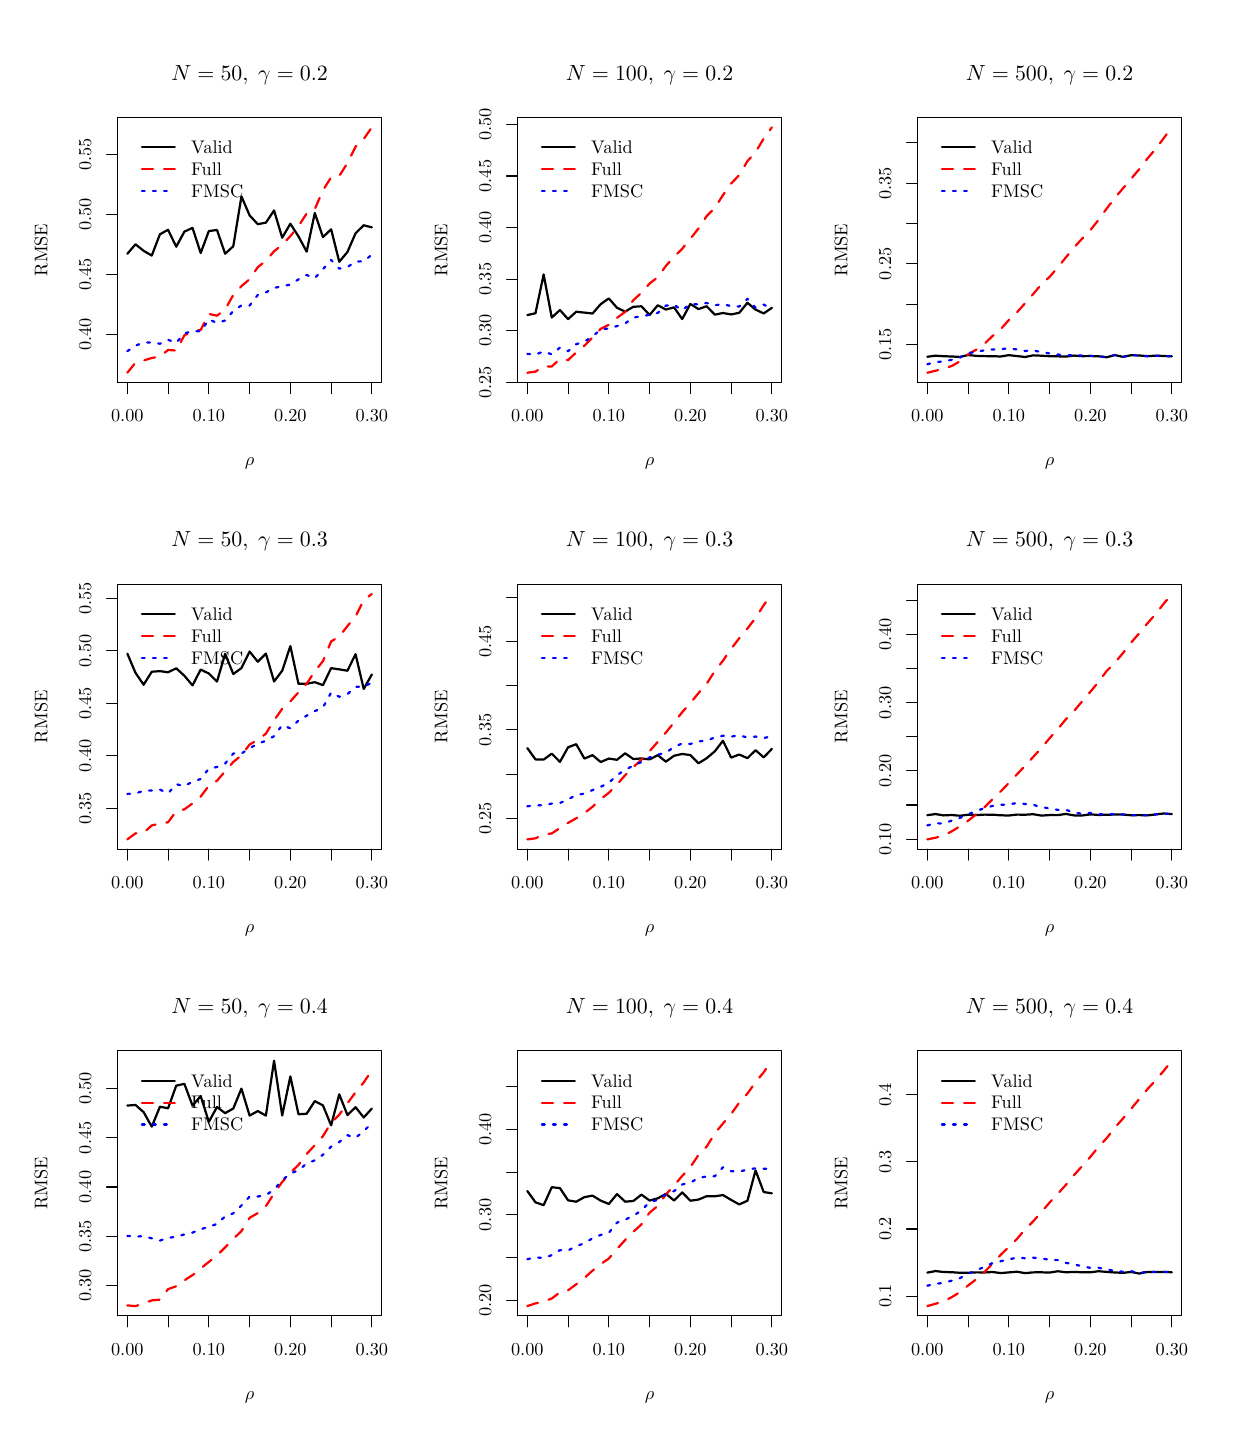
\begin{tikzpicture}[x=1pt,y=1pt]
\definecolor[named]{fillColor}{rgb}{1.00,1.00,1.00}
\path[use as bounding box,fill=fillColor,fill opacity=0.00] (0,0) rectangle (433.62,505.89);
\begin{scope}
\path[clip] ( 32.47,377.65) rectangle (127.91,473.42);
\definecolor[named]{drawColor}{rgb}{0.00,0.00,0.00}

\path[draw=drawColor,line width= 0.8pt,line join=round,line cap=round] ( 36.01,424.15) --
	( 38.95,427.61) --
	( 41.90,425.26) --
	( 44.84,423.54) --
	( 47.79,431.23) --
	( 50.73,432.85) --
	( 53.68,426.73) --
	( 56.63,432.19) --
	( 59.57,433.54) --
	( 62.52,424.45) --
	( 65.46,432.38) --
	( 68.41,432.79) --
	( 71.35,424.19) --
	( 74.30,426.91) --
	( 77.24,444.92) --
	( 80.19,438.07) --
	( 83.14,434.88) --
	( 86.08,435.43) --
	( 89.03,439.83) --
	( 91.97,430.00) --
	( 94.92,435.03) --
	( 97.86,430.45) --
	(100.81,424.95) --
	(103.75,438.92) --
	(106.70,430.21) --
	(109.65,433.03) --
	(112.59,421.28) --
	(115.54,424.82) --
	(118.48,431.58) --
	(121.43,434.49) --
	(124.37,433.72);
\end{scope}
\begin{scope}
\path[clip] (  0.00,  0.00) rectangle (433.62,505.89);
\definecolor[named]{drawColor}{rgb}{0.00,0.00,0.00}

\path[draw=drawColor,line width= 0.4pt,line join=round,line cap=round] ( 36.01,377.65) -- (124.37,377.65);

\path[draw=drawColor,line width= 0.4pt,line join=round,line cap=round] ( 36.01,377.65) -- ( 36.01,373.69);

\path[draw=drawColor,line width= 0.4pt,line join=round,line cap=round] ( 50.73,377.65) -- ( 50.73,373.69);

\path[draw=drawColor,line width= 0.4pt,line join=round,line cap=round] ( 65.46,377.65) -- ( 65.46,373.69);

\path[draw=drawColor,line width= 0.4pt,line join=round,line cap=round] ( 80.19,377.65) -- ( 80.19,373.69);

\path[draw=drawColor,line width= 0.4pt,line join=round,line cap=round] ( 94.92,377.65) -- ( 94.92,373.69);

\path[draw=drawColor,line width= 0.4pt,line join=round,line cap=round] (109.65,377.65) -- (109.65,373.69);

\path[draw=drawColor,line width= 0.4pt,line join=round,line cap=round] (124.37,377.65) -- (124.37,373.69);

\node[text=drawColor,anchor=base,inner sep=0pt, outer sep=0pt, scale=  0.66] at ( 36.01,363.40) {0.00};

\node[text=drawColor,anchor=base,inner sep=0pt, outer sep=0pt, scale=  0.66] at ( 65.46,363.40) {0.10};

\node[text=drawColor,anchor=base,inner sep=0pt, outer sep=0pt, scale=  0.66] at ( 94.92,363.40) {0.20};

\node[text=drawColor,anchor=base,inner sep=0pt, outer sep=0pt, scale=  0.66] at (124.37,363.40) {0.30};

\path[draw=drawColor,line width= 0.4pt,line join=round,line cap=round] ( 32.47,394.97) -- ( 32.47,460.08);

\path[draw=drawColor,line width= 0.4pt,line join=round,line cap=round] ( 32.47,394.97) -- ( 28.51,394.97);

\path[draw=drawColor,line width= 0.4pt,line join=round,line cap=round] ( 32.47,416.68) -- ( 28.51,416.68);

\path[draw=drawColor,line width= 0.4pt,line join=round,line cap=round] ( 32.47,438.38) -- ( 28.51,438.38);

\path[draw=drawColor,line width= 0.4pt,line join=round,line cap=round] ( 32.47,460.08) -- ( 28.51,460.08);

\node[text=drawColor,rotate= 90.00,anchor=base,inner sep=0pt, outer sep=0pt, scale=  0.66] at ( 22.97,394.97) {0.40};

\node[text=drawColor,rotate= 90.00,anchor=base,inner sep=0pt, outer sep=0pt, scale=  0.66] at ( 22.97,416.68) {0.45};

\node[text=drawColor,rotate= 90.00,anchor=base,inner sep=0pt, outer sep=0pt, scale=  0.66] at ( 22.97,438.38) {0.50};

\node[text=drawColor,rotate= 90.00,anchor=base,inner sep=0pt, outer sep=0pt, scale=  0.66] at ( 22.97,460.08) {0.55};

\path[draw=drawColor,line width= 0.4pt,line join=round,line cap=round] ( 32.47,377.65) --
	(127.91,377.65) --
	(127.91,473.42) --
	( 32.47,473.42) --
	( 32.47,377.65);
\end{scope}
\begin{scope}
\path[clip] (  0.00,337.26) rectangle (144.54,505.89);
\definecolor[named]{drawColor}{rgb}{0.00,0.00,0.00}

\node[text=drawColor,anchor=base,inner sep=0pt, outer sep=0pt, scale=  0.79] at ( 80.19,486.92) {\bfseries $N=50, \;\gamma=0.2$};

\node[text=drawColor,anchor=base,inner sep=0pt, outer sep=0pt, scale=  0.66] at ( 80.19,347.56) {$\rho$};

\node[text=drawColor,rotate= 90.00,anchor=base,inner sep=0pt, outer sep=0pt, scale=  0.66] at (  7.13,425.53) {RMSE};
\end{scope}
\begin{scope}
\path[clip] ( 32.47,377.65) rectangle (127.91,473.42);
\definecolor[named]{drawColor}{rgb}{1.00,0.00,0.00}

\path[draw=drawColor,line width= 0.8pt,dash pattern=on 4pt off 4pt ,line join=round,line cap=round] ( 36.01,381.20) --
	( 38.95,384.82) --
	( 41.90,385.63) --
	( 44.84,386.53) --
	( 47.79,387.02) --
	( 50.73,389.43) --
	( 53.68,389.21) --
	( 56.63,394.72) --
	( 59.57,396.22) --
	( 62.52,396.63) --
	( 65.46,402.46) --
	( 68.41,401.81) --
	( 71.35,404.07) --
	( 74.30,409.29) --
	( 77.24,412.47) --
	( 80.19,414.99) --
	( 83.14,419.35) --
	( 86.08,421.65) --
	( 89.03,425.08) --
	( 91.97,427.42) --
	( 94.92,430.56) --
	( 97.86,434.17) --
	(100.81,438.75) --
	(103.75,440.32) --
	(106.70,447.14) --
	(109.65,451.81) --
	(112.59,452.27) --
	(115.54,456.97) --
	(118.48,462.88) --
	(121.43,465.66) --
	(124.37,469.87);
\definecolor[named]{drawColor}{rgb}{0.00,0.00,1.00}

\path[draw=drawColor,line width= 0.8pt,dash pattern=on 1pt off 3pt ,line join=round,line cap=round] ( 36.01,388.99) --
	( 38.95,390.97) --
	( 41.90,392.10) --
	( 44.84,392.17) --
	( 47.79,391.68) --
	( 50.73,393.09) --
	( 53.68,392.01) --
	( 56.63,395.37) --
	( 59.57,396.31) --
	( 62.52,396.11) --
	( 65.46,400.43) --
	( 68.41,399.21) --
	( 71.35,400.06) --
	( 74.30,403.53) --
	( 77.24,405.51) --
	( 80.19,405.47) --
	( 83.14,409.29) --
	( 86.08,410.22) --
	( 89.03,411.89) --
	( 91.97,412.38) --
	( 94.92,413.08) --
	( 97.86,414.92) --
	(100.81,416.51) --
	(103.75,415.38) --
	(106.70,418.59) --
	(109.65,421.96) --
	(112.59,418.82) --
	(115.54,419.37) --
	(118.48,421.38) --
	(121.43,421.48) --
	(124.37,423.84);
\definecolor[named]{drawColor}{rgb}{0.00,0.00,0.00}

\path[draw=drawColor,line width= 0.8pt,line join=round,line cap=round] ( 41.28,462.63) -- ( 53.16,462.63);
\definecolor[named]{drawColor}{rgb}{1.00,0.00,0.00}

\path[draw=drawColor,line width= 0.8pt,dash pattern=on 4pt off 4pt ,line join=round,line cap=round] ( 41.28,454.71) -- ( 53.16,454.71);
\definecolor[named]{drawColor}{rgb}{0.00,0.00,1.00}

\path[draw=drawColor,line width= 0.8pt,dash pattern=on 1pt off 3pt ,line join=round,line cap=round] ( 41.28,446.79) -- ( 53.16,446.79);
\definecolor[named]{drawColor}{rgb}{0.00,0.00,0.00}

\node[text=drawColor,anchor=base west,inner sep=0pt, outer sep=0pt, scale=  0.66] at ( 59.10,460.35) {Valid};

\node[text=drawColor,anchor=base west,inner sep=0pt, outer sep=0pt, scale=  0.66] at ( 59.10,452.43) {Full};

\node[text=drawColor,anchor=base west,inner sep=0pt, outer sep=0pt, scale=  0.66] at ( 59.10,444.51) {FMSC};
\end{scope}
\begin{scope}
\path[clip] (177.01,377.65) rectangle (272.45,473.42);
\definecolor[named]{drawColor}{rgb}{0.00,0.00,0.00}

\path[draw=drawColor,line width= 0.8pt,line join=round,line cap=round] (180.55,402.03) --
	(183.49,402.69) --
	(186.44,416.70) --
	(189.38,401.13) --
	(192.33,403.85) --
	(195.27,400.57) --
	(198.22,403.24) --
	(201.17,402.93) --
	(204.11,402.60) --
	(207.06,405.98) --
	(210.00,408.05) --
	(212.95,404.67) --
	(215.89,403.28) --
	(218.84,405.02) --
	(221.78,405.21) --
	(224.73,402.06) --
	(227.68,405.58) --
	(230.62,404.03) --
	(233.57,404.82) --
	(236.51,400.59) --
	(239.46,406.05) --
	(242.40,404.20) --
	(245.35,405.23) --
	(248.29,402.19) --
	(251.24,402.77) --
	(254.19,402.27) --
	(257.13,402.86) --
	(260.08,406.47) --
	(263.02,404.02) --
	(265.97,402.62) --
	(268.91,404.65);
\end{scope}
\begin{scope}
\path[clip] (  0.00,  0.00) rectangle (433.62,505.89);
\definecolor[named]{drawColor}{rgb}{0.00,0.00,0.00}

\path[draw=drawColor,line width= 0.4pt,line join=round,line cap=round] (180.55,377.65) -- (268.91,377.65);

\path[draw=drawColor,line width= 0.4pt,line join=round,line cap=round] (180.55,377.65) -- (180.55,373.69);

\path[draw=drawColor,line width= 0.4pt,line join=round,line cap=round] (195.27,377.65) -- (195.27,373.69);

\path[draw=drawColor,line width= 0.4pt,line join=round,line cap=round] (210.00,377.65) -- (210.00,373.69);

\path[draw=drawColor,line width= 0.4pt,line join=round,line cap=round] (224.73,377.65) -- (224.73,373.69);

\path[draw=drawColor,line width= 0.4pt,line join=round,line cap=round] (239.46,377.65) -- (239.46,373.69);

\path[draw=drawColor,line width= 0.4pt,line join=round,line cap=round] (254.19,377.65) -- (254.19,373.69);

\path[draw=drawColor,line width= 0.4pt,line join=round,line cap=round] (268.91,377.65) -- (268.91,373.69);

\node[text=drawColor,anchor=base,inner sep=0pt, outer sep=0pt, scale=  0.66] at (180.55,363.40) {0.00};

\node[text=drawColor,anchor=base,inner sep=0pt, outer sep=0pt, scale=  0.66] at (210.00,363.40) {0.10};

\node[text=drawColor,anchor=base,inner sep=0pt, outer sep=0pt, scale=  0.66] at (239.46,363.40) {0.20};

\node[text=drawColor,anchor=base,inner sep=0pt, outer sep=0pt, scale=  0.66] at (268.91,363.40) {0.30};

\path[draw=drawColor,line width= 0.4pt,line join=round,line cap=round] (177.01,377.81) -- (177.01,470.89);

\path[draw=drawColor,line width= 0.4pt,line join=round,line cap=round] (177.01,377.81) -- (173.05,377.81);

\path[draw=drawColor,line width= 0.4pt,line join=round,line cap=round] (177.01,396.42) -- (173.05,396.42);

\path[draw=drawColor,line width= 0.4pt,line join=round,line cap=round] (177.01,415.04) -- (173.05,415.04);

\path[draw=drawColor,line width= 0.4pt,line join=round,line cap=round] (177.01,433.66) -- (173.05,433.66);

\path[draw=drawColor,line width= 0.4pt,line join=round,line cap=round] (177.01,452.27) -- (173.05,452.27);

\path[draw=drawColor,line width= 0.4pt,line join=round,line cap=round] (177.01,470.89) -- (173.05,470.89);

\node[text=drawColor,rotate= 90.00,anchor=base,inner sep=0pt, outer sep=0pt, scale=  0.66] at (167.51,377.81) {0.25};

\node[text=drawColor,rotate= 90.00,anchor=base,inner sep=0pt, outer sep=0pt, scale=  0.66] at (167.51,396.42) {0.30};

\node[text=drawColor,rotate= 90.00,anchor=base,inner sep=0pt, outer sep=0pt, scale=  0.66] at (167.51,415.04) {0.35};

\node[text=drawColor,rotate= 90.00,anchor=base,inner sep=0pt, outer sep=0pt, scale=  0.66] at (167.51,433.66) {0.40};

\node[text=drawColor,rotate= 90.00,anchor=base,inner sep=0pt, outer sep=0pt, scale=  0.66] at (167.51,452.27) {0.45};

\node[text=drawColor,rotate= 90.00,anchor=base,inner sep=0pt, outer sep=0pt, scale=  0.66] at (167.51,470.89) {0.50};

\path[draw=drawColor,line width= 0.4pt,line join=round,line cap=round] (177.01,377.65) --
	(272.45,377.65) --
	(272.45,473.42) --
	(177.01,473.42) --
	(177.01,377.65);
\end{scope}
\begin{scope}
\path[clip] (144.54,337.26) rectangle (289.08,505.89);
\definecolor[named]{drawColor}{rgb}{0.00,0.00,0.00}

\node[text=drawColor,anchor=base,inner sep=0pt, outer sep=0pt, scale=  0.79] at (224.73,486.92) {\bfseries $N=100, \;\gamma=0.2$};

\node[text=drawColor,anchor=base,inner sep=0pt, outer sep=0pt, scale=  0.66] at (224.73,347.56) {$\rho$};

\node[text=drawColor,rotate= 90.00,anchor=base,inner sep=0pt, outer sep=0pt, scale=  0.66] at (151.67,425.53) {RMSE};
\end{scope}
\begin{scope}
\path[clip] (177.01,377.65) rectangle (272.45,473.42);
\definecolor[named]{drawColor}{rgb}{1.00,0.00,0.00}

\path[draw=drawColor,line width= 0.8pt,dash pattern=on 4pt off 4pt ,line join=round,line cap=round] (180.55,381.20) --
	(183.49,381.58) --
	(186.44,383.54) --
	(189.38,383.44) --
	(192.33,386.21) --
	(195.27,385.76) --
	(198.22,388.57) --
	(201.17,390.96) --
	(204.11,393.95) --
	(207.06,397.06) --
	(210.00,398.51) --
	(212.95,401.03) --
	(215.89,403.20) --
	(218.84,407.40) --
	(221.78,410.07) --
	(224.73,413.43) --
	(227.68,415.73) --
	(230.62,419.81) --
	(233.57,423.09) --
	(236.51,425.98) --
	(239.46,429.63) --
	(242.40,433.31) --
	(245.35,437.80) --
	(248.29,440.75) --
	(251.24,445.38) --
	(254.19,449.54) --
	(257.13,452.66) --
	(260.08,457.65) --
	(263.02,460.92) --
	(265.97,465.81) --
	(268.91,469.87);
\definecolor[named]{drawColor}{rgb}{0.00,0.00,1.00}

\path[draw=drawColor,line width= 0.8pt,dash pattern=on 1pt off 3pt ,line join=round,line cap=round] (180.55,388.00) --
	(183.49,387.77) --
	(186.44,388.89) --
	(189.38,387.83) --
	(192.33,390.28) --
	(195.27,388.99) --
	(198.22,391.51) --
	(201.17,392.44) --
	(204.11,394.33) --
	(207.06,396.81) --
	(210.00,397.22) --
	(212.95,398.05) --
	(215.89,399.02) --
	(218.84,401.12) --
	(221.78,401.60) --
	(224.73,402.12) --
	(227.68,402.81) --
	(230.62,405.46) --
	(233.57,405.72) --
	(236.51,403.76) --
	(239.46,406.11) --
	(242.40,405.85) --
	(245.35,406.41) --
	(248.29,405.56) --
	(251.24,406.04) --
	(254.19,405.23) --
	(257.13,405.15) --
	(260.08,407.91) --
	(263.02,404.68) --
	(265.97,405.82) --
	(268.91,404.25);
\definecolor[named]{drawColor}{rgb}{0.00,0.00,0.00}

\path[draw=drawColor,line width= 0.8pt,line join=round,line cap=round] (185.82,462.63) -- (197.70,462.63);
\definecolor[named]{drawColor}{rgb}{1.00,0.00,0.00}

\path[draw=drawColor,line width= 0.8pt,dash pattern=on 4pt off 4pt ,line join=round,line cap=round] (185.82,454.71) -- (197.70,454.71);
\definecolor[named]{drawColor}{rgb}{0.00,0.00,1.00}

\path[draw=drawColor,line width= 0.8pt,dash pattern=on 1pt off 3pt ,line join=round,line cap=round] (185.82,446.79) -- (197.70,446.79);
\definecolor[named]{drawColor}{rgb}{0.00,0.00,0.00}

\node[text=drawColor,anchor=base west,inner sep=0pt, outer sep=0pt, scale=  0.66] at (203.64,460.35) {Valid};

\node[text=drawColor,anchor=base west,inner sep=0pt, outer sep=0pt, scale=  0.66] at (203.64,452.43) {Full};

\node[text=drawColor,anchor=base west,inner sep=0pt, outer sep=0pt, scale=  0.66] at (203.64,444.51) {FMSC};
\end{scope}
\begin{scope}
\path[clip] (321.55,377.65) rectangle (416.99,473.42);
\definecolor[named]{drawColor}{rgb}{0.00,0.00,0.00}

\path[draw=drawColor,line width= 0.8pt,line join=round,line cap=round] (325.09,386.97) --
	(328.03,387.36) --
	(330.98,387.16) --
	(333.92,387.07) --
	(336.87,386.91) --
	(339.81,387.59) --
	(342.76,387.30) --
	(345.71,387.20) --
	(348.65,387.17) --
	(351.60,387.07) --
	(354.54,387.55) --
	(357.49,387.22) --
	(360.43,386.89) --
	(363.38,387.48) --
	(366.32,387.35) --
	(369.27,387.16) --
	(372.22,387.12) --
	(375.16,387.03) --
	(378.11,387.39) --
	(381.05,387.18) --
	(384.00,387.22) --
	(386.94,387.14) --
	(389.89,386.78) --
	(392.83,387.58) --
	(395.78,386.93) --
	(398.73,387.53) --
	(401.67,387.43) --
	(404.62,387.18) --
	(407.56,387.37) --
	(410.51,387.24) --
	(413.45,387.13);
\end{scope}
\begin{scope}
\path[clip] (  0.00,  0.00) rectangle (433.62,505.89);
\definecolor[named]{drawColor}{rgb}{0.00,0.00,0.00}

\path[draw=drawColor,line width= 0.4pt,line join=round,line cap=round] (325.09,377.65) -- (413.45,377.65);

\path[draw=drawColor,line width= 0.4pt,line join=round,line cap=round] (325.09,377.65) -- (325.09,373.69);

\path[draw=drawColor,line width= 0.4pt,line join=round,line cap=round] (339.81,377.65) -- (339.81,373.69);

\path[draw=drawColor,line width= 0.4pt,line join=round,line cap=round] (354.54,377.65) -- (354.54,373.69);

\path[draw=drawColor,line width= 0.4pt,line join=round,line cap=round] (369.27,377.65) -- (369.27,373.69);

\path[draw=drawColor,line width= 0.4pt,line join=round,line cap=round] (384.00,377.65) -- (384.00,373.69);

\path[draw=drawColor,line width= 0.4pt,line join=round,line cap=round] (398.73,377.65) -- (398.73,373.69);

\path[draw=drawColor,line width= 0.4pt,line join=round,line cap=round] (413.45,377.65) -- (413.45,373.69);

\node[text=drawColor,anchor=base,inner sep=0pt, outer sep=0pt, scale=  0.66] at (325.09,363.40) {0.00};

\node[text=drawColor,anchor=base,inner sep=0pt, outer sep=0pt, scale=  0.66] at (354.54,363.40) {0.10};

\node[text=drawColor,anchor=base,inner sep=0pt, outer sep=0pt, scale=  0.66] at (384.00,363.40) {0.20};

\node[text=drawColor,anchor=base,inner sep=0pt, outer sep=0pt, scale=  0.66] at (413.45,363.40) {0.30};

\path[draw=drawColor,line width= 0.4pt,line join=round,line cap=round] (321.55,391.42) -- (321.55,464.29);

\path[draw=drawColor,line width= 0.4pt,line join=round,line cap=round] (321.55,391.42) -- (317.59,391.42);

\path[draw=drawColor,line width= 0.4pt,line join=round,line cap=round] (321.55,405.99) -- (317.59,405.99);

\path[draw=drawColor,line width= 0.4pt,line join=round,line cap=round] (321.55,420.57) -- (317.59,420.57);

\path[draw=drawColor,line width= 0.4pt,line join=round,line cap=round] (321.55,435.14) -- (317.59,435.14);

\path[draw=drawColor,line width= 0.4pt,line join=round,line cap=round] (321.55,449.71) -- (317.59,449.71);

\path[draw=drawColor,line width= 0.4pt,line join=round,line cap=round] (321.55,464.29) -- (317.59,464.29);

\node[text=drawColor,rotate= 90.00,anchor=base,inner sep=0pt, outer sep=0pt, scale=  0.66] at (312.05,391.42) {0.15};

\node[text=drawColor,rotate= 90.00,anchor=base,inner sep=0pt, outer sep=0pt, scale=  0.66] at (312.05,420.57) {0.25};

\node[text=drawColor,rotate= 90.00,anchor=base,inner sep=0pt, outer sep=0pt, scale=  0.66] at (312.05,449.71) {0.35};

\path[draw=drawColor,line width= 0.4pt,line join=round,line cap=round] (321.55,377.65) --
	(416.99,377.65) --
	(416.99,473.42) --
	(321.55,473.42) --
	(321.55,377.65);
\end{scope}
\begin{scope}
\path[clip] (289.08,337.26) rectangle (433.62,505.89);
\definecolor[named]{drawColor}{rgb}{0.00,0.00,0.00}

\node[text=drawColor,anchor=base,inner sep=0pt, outer sep=0pt, scale=  0.79] at (369.27,486.92) {\bfseries $N=500, \;\gamma=0.2$};

\node[text=drawColor,anchor=base,inner sep=0pt, outer sep=0pt, scale=  0.66] at (369.27,347.56) {$\rho$};

\node[text=drawColor,rotate= 90.00,anchor=base,inner sep=0pt, outer sep=0pt, scale=  0.66] at (296.21,425.53) {RMSE};
\end{scope}
\begin{scope}
\path[clip] (321.55,377.65) rectangle (416.99,473.42);
\definecolor[named]{drawColor}{rgb}{1.00,0.00,0.00}

\path[draw=drawColor,line width= 0.8pt,dash pattern=on 4pt off 4pt ,line join=round,line cap=round] (325.09,381.20) --
	(328.03,381.90) --
	(330.98,382.64) --
	(333.92,383.64) --
	(336.87,385.33) --
	(339.81,387.85) --
	(342.76,389.53) --
	(345.71,391.62) --
	(348.65,394.48) --
	(351.60,396.91) --
	(354.54,400.25) --
	(357.49,403.07) --
	(360.43,406.33) --
	(363.38,409.68) --
	(366.32,413.18) --
	(369.27,415.82) --
	(372.22,419.24) --
	(375.16,422.89) --
	(378.11,426.44) --
	(381.05,429.68) --
	(384.00,432.72) --
	(386.94,436.41) --
	(389.89,440.52) --
	(392.83,444.32) --
	(395.78,447.82) --
	(398.73,451.30) --
	(401.67,454.76) --
	(404.62,458.59) --
	(407.56,462.04) --
	(410.51,465.97) --
	(413.45,469.87);
\definecolor[named]{drawColor}{rgb}{0.00,0.00,1.00}

\path[draw=drawColor,line width= 0.8pt,dash pattern=on 1pt off 3pt ,line join=round,line cap=round] (325.09,384.27) --
	(328.03,385.01) --
	(330.98,385.31) --
	(333.92,385.85) --
	(336.87,386.72) --
	(339.81,388.28) --
	(342.76,388.72) --
	(345.71,389.31) --
	(348.65,389.60) --
	(351.60,389.66) --
	(354.54,390.10) --
	(357.49,389.58) --
	(360.43,389.08) --
	(363.38,389.20) --
	(366.32,388.69) --
	(369.27,388.16) --
	(372.22,387.78) --
	(375.16,387.40) --
	(378.11,387.66) --
	(381.05,387.39) --
	(384.00,387.30) --
	(386.94,387.20) --
	(389.89,386.79) --
	(392.83,387.59) --
	(395.78,386.93) --
	(398.73,387.53) --
	(401.67,387.43) --
	(404.62,387.18) --
	(407.56,387.37) --
	(410.51,387.24) --
	(413.45,387.13);
\definecolor[named]{drawColor}{rgb}{0.00,0.00,0.00}

\path[draw=drawColor,line width= 0.8pt,line join=round,line cap=round] (330.36,462.63) -- (342.24,462.63);
\definecolor[named]{drawColor}{rgb}{1.00,0.00,0.00}

\path[draw=drawColor,line width= 0.8pt,dash pattern=on 4pt off 4pt ,line join=round,line cap=round] (330.36,454.71) -- (342.24,454.71);
\definecolor[named]{drawColor}{rgb}{0.00,0.00,1.00}

\path[draw=drawColor,line width= 0.8pt,dash pattern=on 1pt off 3pt ,line join=round,line cap=round] (330.36,446.79) -- (342.24,446.79);
\definecolor[named]{drawColor}{rgb}{0.00,0.00,0.00}

\node[text=drawColor,anchor=base west,inner sep=0pt, outer sep=0pt, scale=  0.66] at (348.18,460.35) {Valid};

\node[text=drawColor,anchor=base west,inner sep=0pt, outer sep=0pt, scale=  0.66] at (348.18,452.43) {Full};

\node[text=drawColor,anchor=base west,inner sep=0pt, outer sep=0pt, scale=  0.66] at (348.18,444.51) {FMSC};
\end{scope}
\begin{scope}
\path[clip] ( 32.47,209.02) rectangle (127.91,304.79);
\definecolor[named]{drawColor}{rgb}{0.00,0.00,0.00}

\path[draw=drawColor,line width= 0.8pt,line join=round,line cap=round] ( 36.01,279.71) --
	( 38.95,272.76) --
	( 41.90,268.46) --
	( 44.84,273.16) --
	( 47.79,273.37) --
	( 50.73,272.95) --
	( 53.68,274.40) --
	( 56.63,271.70) --
	( 59.57,268.22) --
	( 62.52,273.95) --
	( 65.46,272.51) --
	( 68.41,269.58) --
	( 71.35,279.63) --
	( 74.30,272.32) --
	( 77.24,274.48) --
	( 80.19,280.45) --
	( 83.14,276.77) --
	( 86.08,279.72) --
	( 89.03,269.63) --
	( 91.97,273.52) --
	( 94.92,282.41) --
	( 97.86,268.78) --
	(100.81,268.81) --
	(103.75,269.38) --
	(106.70,268.32) --
	(109.65,274.45) --
	(112.59,274.01) --
	(115.54,273.52) --
	(118.48,279.49) --
	(121.43,266.94) --
	(124.37,272.17);
\end{scope}
\begin{scope}
\path[clip] (  0.00,  0.00) rectangle (433.62,505.89);
\definecolor[named]{drawColor}{rgb}{0.00,0.00,0.00}

\path[draw=drawColor,line width= 0.4pt,line join=round,line cap=round] ( 36.01,209.02) -- (124.37,209.02);

\path[draw=drawColor,line width= 0.4pt,line join=round,line cap=round] ( 36.01,209.02) -- ( 36.01,205.06);

\path[draw=drawColor,line width= 0.4pt,line join=round,line cap=round] ( 50.73,209.02) -- ( 50.73,205.06);

\path[draw=drawColor,line width= 0.4pt,line join=round,line cap=round] ( 65.46,209.02) -- ( 65.46,205.06);

\path[draw=drawColor,line width= 0.4pt,line join=round,line cap=round] ( 80.19,209.02) -- ( 80.19,205.06);

\path[draw=drawColor,line width= 0.4pt,line join=round,line cap=round] ( 94.92,209.02) -- ( 94.92,205.06);

\path[draw=drawColor,line width= 0.4pt,line join=round,line cap=round] (109.65,209.02) -- (109.65,205.06);

\path[draw=drawColor,line width= 0.4pt,line join=round,line cap=round] (124.37,209.02) -- (124.37,205.06);

\node[text=drawColor,anchor=base,inner sep=0pt, outer sep=0pt, scale=  0.66] at ( 36.01,194.77) {0.00};

\node[text=drawColor,anchor=base,inner sep=0pt, outer sep=0pt, scale=  0.66] at ( 65.46,194.77) {0.10};

\node[text=drawColor,anchor=base,inner sep=0pt, outer sep=0pt, scale=  0.66] at ( 94.92,194.77) {0.20};

\node[text=drawColor,anchor=base,inner sep=0pt, outer sep=0pt, scale=  0.66] at (124.37,194.77) {0.30};

\path[draw=drawColor,line width= 0.4pt,line join=round,line cap=round] ( 32.47,223.84) -- ( 32.47,299.62);

\path[draw=drawColor,line width= 0.4pt,line join=round,line cap=round] ( 32.47,223.84) -- ( 28.51,223.84);

\path[draw=drawColor,line width= 0.4pt,line join=round,line cap=round] ( 32.47,242.79) -- ( 28.51,242.79);

\path[draw=drawColor,line width= 0.4pt,line join=round,line cap=round] ( 32.47,261.73) -- ( 28.51,261.73);

\path[draw=drawColor,line width= 0.4pt,line join=round,line cap=round] ( 32.47,280.67) -- ( 28.51,280.67);

\path[draw=drawColor,line width= 0.4pt,line join=round,line cap=round] ( 32.47,299.62) -- ( 28.51,299.62);

\node[text=drawColor,rotate= 90.00,anchor=base,inner sep=0pt, outer sep=0pt, scale=  0.66] at ( 22.97,223.84) {0.35};

\node[text=drawColor,rotate= 90.00,anchor=base,inner sep=0pt, outer sep=0pt, scale=  0.66] at ( 22.97,242.79) {0.40};

\node[text=drawColor,rotate= 90.00,anchor=base,inner sep=0pt, outer sep=0pt, scale=  0.66] at ( 22.97,261.73) {0.45};

\node[text=drawColor,rotate= 90.00,anchor=base,inner sep=0pt, outer sep=0pt, scale=  0.66] at ( 22.97,280.67) {0.50};

\node[text=drawColor,rotate= 90.00,anchor=base,inner sep=0pt, outer sep=0pt, scale=  0.66] at ( 22.97,299.62) {0.55};

\path[draw=drawColor,line width= 0.4pt,line join=round,line cap=round] ( 32.47,209.02) --
	(127.91,209.02) --
	(127.91,304.79) --
	( 32.47,304.79) --
	( 32.47,209.02);
\end{scope}
\begin{scope}
\path[clip] (  0.00,168.63) rectangle (144.54,337.26);
\definecolor[named]{drawColor}{rgb}{0.00,0.00,0.00}

\node[text=drawColor,anchor=base,inner sep=0pt, outer sep=0pt, scale=  0.79] at ( 80.19,318.29) {\bfseries $N=50, \;\gamma=0.3$};

\node[text=drawColor,anchor=base,inner sep=0pt, outer sep=0pt, scale=  0.66] at ( 80.19,178.93) {$\rho$};

\node[text=drawColor,rotate= 90.00,anchor=base,inner sep=0pt, outer sep=0pt, scale=  0.66] at (  7.13,256.90) {RMSE};
\end{scope}
\begin{scope}
\path[clip] ( 32.47,209.02) rectangle (127.91,304.79);
\definecolor[named]{drawColor}{rgb}{1.00,0.00,0.00}

\path[draw=drawColor,line width= 0.8pt,dash pattern=on 4pt off 4pt ,line join=round,line cap=round] ( 36.01,212.57) --
	( 38.95,214.75) --
	( 41.90,214.90) --
	( 44.84,217.63) --
	( 47.79,218.28) --
	( 50.73,218.75) --
	( 53.68,222.75) --
	( 56.63,223.43) --
	( 59.57,225.59) --
	( 62.52,228.05) --
	( 65.46,231.95) --
	( 68.41,233.76) --
	( 71.35,237.19) --
	( 74.30,240.56) --
	( 77.24,242.94) --
	( 80.19,246.86) --
	( 83.14,248.52) --
	( 86.08,250.79) --
	( 89.03,255.59) --
	( 91.97,259.76) --
	( 94.92,262.43) --
	( 97.86,265.74) --
	(100.81,268.82) --
	(103.75,273.30) --
	(106.70,276.98) --
	(109.65,284.09) --
	(112.59,285.89) --
	(115.54,289.65) --
	(118.48,293.08) --
	(121.43,299.01) --
	(124.37,301.24);
\definecolor[named]{drawColor}{rgb}{0.00,0.00,1.00}

\path[draw=drawColor,line width= 0.8pt,dash pattern=on 1pt off 3pt ,line join=round,line cap=round] ( 36.01,228.99) --
	( 38.95,229.22) --
	( 41.90,230.08) --
	( 44.84,230.24) --
	( 47.79,230.56) --
	( 50.73,229.22) --
	( 53.68,232.50) --
	( 56.63,231.84) --
	( 59.57,233.42) --
	( 62.52,234.39) --
	( 65.46,238.13) --
	( 68.41,238.74) --
	( 71.35,239.99) --
	( 74.30,243.59) --
	( 77.24,243.60) --
	( 80.19,245.51) --
	( 83.14,247.14) --
	( 86.08,248.20) --
	( 89.03,249.87) --
	( 91.97,253.86) --
	( 94.92,252.70) --
	( 97.86,255.53) --
	(100.81,257.28) --
	(103.75,258.92) --
	(106.70,260.25) --
	(109.65,265.62) --
	(112.59,264.11) --
	(115.54,265.05) --
	(118.48,267.68) --
	(121.43,267.82) --
	(124.37,269.14);
\definecolor[named]{drawColor}{rgb}{0.00,0.00,0.00}

\path[draw=drawColor,line width= 0.8pt,line join=round,line cap=round] ( 41.28,294.00) -- ( 53.16,294.00);
\definecolor[named]{drawColor}{rgb}{1.00,0.00,0.00}

\path[draw=drawColor,line width= 0.8pt,dash pattern=on 4pt off 4pt ,line join=round,line cap=round] ( 41.28,286.08) -- ( 53.16,286.08);
\definecolor[named]{drawColor}{rgb}{0.00,0.00,1.00}

\path[draw=drawColor,line width= 0.8pt,dash pattern=on 1pt off 3pt ,line join=round,line cap=round] ( 41.28,278.16) -- ( 53.16,278.16);
\definecolor[named]{drawColor}{rgb}{0.00,0.00,0.00}

\node[text=drawColor,anchor=base west,inner sep=0pt, outer sep=0pt, scale=  0.66] at ( 59.10,291.72) {Valid};

\node[text=drawColor,anchor=base west,inner sep=0pt, outer sep=0pt, scale=  0.66] at ( 59.10,283.80) {Full};

\node[text=drawColor,anchor=base west,inner sep=0pt, outer sep=0pt, scale=  0.66] at ( 59.10,275.88) {FMSC};
\end{scope}
\begin{scope}
\path[clip] (177.01,209.02) rectangle (272.45,304.79);
\definecolor[named]{drawColor}{rgb}{0.00,0.00,0.00}

\path[draw=drawColor,line width= 0.8pt,line join=round,line cap=round] (180.55,245.57) --
	(183.49,241.48) --
	(186.44,241.41) --
	(189.38,243.55) --
	(192.33,240.58) --
	(195.27,245.86) --
	(198.22,246.97) --
	(201.17,241.78) --
	(204.11,243.01) --
	(207.06,240.53) --
	(210.00,241.78) --
	(212.95,241.33) --
	(215.89,243.69) --
	(218.84,241.62) --
	(221.78,241.81) --
	(224.73,241.48) --
	(227.68,243.01) --
	(230.62,240.66) --
	(233.57,242.80) --
	(236.51,243.44) --
	(239.46,243.04) --
	(242.40,240.08) --
	(245.35,241.90) --
	(248.29,244.40) --
	(251.24,248.20) --
	(254.19,242.13) --
	(257.13,243.23) --
	(260.08,241.93) --
	(263.02,244.80) --
	(265.97,242.20) --
	(268.91,245.28);
\end{scope}
\begin{scope}
\path[clip] (  0.00,  0.00) rectangle (433.62,505.89);
\definecolor[named]{drawColor}{rgb}{0.00,0.00,0.00}

\path[draw=drawColor,line width= 0.4pt,line join=round,line cap=round] (180.55,209.02) -- (268.91,209.02);

\path[draw=drawColor,line width= 0.4pt,line join=round,line cap=round] (180.55,209.02) -- (180.55,205.06);

\path[draw=drawColor,line width= 0.4pt,line join=round,line cap=round] (195.27,209.02) -- (195.27,205.06);

\path[draw=drawColor,line width= 0.4pt,line join=round,line cap=round] (210.00,209.02) -- (210.00,205.06);

\path[draw=drawColor,line width= 0.4pt,line join=round,line cap=round] (224.73,209.02) -- (224.73,205.06);

\path[draw=drawColor,line width= 0.4pt,line join=round,line cap=round] (239.46,209.02) -- (239.46,205.06);

\path[draw=drawColor,line width= 0.4pt,line join=round,line cap=round] (254.19,209.02) -- (254.19,205.06);

\path[draw=drawColor,line width= 0.4pt,line join=round,line cap=round] (268.91,209.02) -- (268.91,205.06);

\node[text=drawColor,anchor=base,inner sep=0pt, outer sep=0pt, scale=  0.66] at (180.55,194.77) {0.00};

\node[text=drawColor,anchor=base,inner sep=0pt, outer sep=0pt, scale=  0.66] at (210.00,194.77) {0.10};

\node[text=drawColor,anchor=base,inner sep=0pt, outer sep=0pt, scale=  0.66] at (239.46,194.77) {0.20};

\node[text=drawColor,anchor=base,inner sep=0pt, outer sep=0pt, scale=  0.66] at (268.91,194.77) {0.30};

\path[draw=drawColor,line width= 0.4pt,line join=round,line cap=round] (177.01,220.23) -- (177.01,299.96);

\path[draw=drawColor,line width= 0.4pt,line join=round,line cap=round] (177.01,220.23) -- (173.05,220.23);

\path[draw=drawColor,line width= 0.4pt,line join=round,line cap=round] (177.01,236.18) -- (173.05,236.18);

\path[draw=drawColor,line width= 0.4pt,line join=round,line cap=round] (177.01,252.13) -- (173.05,252.13);

\path[draw=drawColor,line width= 0.4pt,line join=round,line cap=round] (177.01,268.07) -- (173.05,268.07);

\path[draw=drawColor,line width= 0.4pt,line join=round,line cap=round] (177.01,284.02) -- (173.05,284.02);

\path[draw=drawColor,line width= 0.4pt,line join=round,line cap=round] (177.01,299.96) -- (173.05,299.96);

\node[text=drawColor,rotate= 90.00,anchor=base,inner sep=0pt, outer sep=0pt, scale=  0.66] at (167.51,220.23) {0.25};

\node[text=drawColor,rotate= 90.00,anchor=base,inner sep=0pt, outer sep=0pt, scale=  0.66] at (167.51,252.13) {0.35};

\node[text=drawColor,rotate= 90.00,anchor=base,inner sep=0pt, outer sep=0pt, scale=  0.66] at (167.51,284.02) {0.45};

\path[draw=drawColor,line width= 0.4pt,line join=round,line cap=round] (177.01,209.02) --
	(272.45,209.02) --
	(272.45,304.79) --
	(177.01,304.79) --
	(177.01,209.02);
\end{scope}
\begin{scope}
\path[clip] (144.54,168.63) rectangle (289.08,337.26);
\definecolor[named]{drawColor}{rgb}{0.00,0.00,0.00}

\node[text=drawColor,anchor=base,inner sep=0pt, outer sep=0pt, scale=  0.79] at (224.73,318.29) {\bfseries $N=100, \;\gamma=0.3$};

\node[text=drawColor,anchor=base,inner sep=0pt, outer sep=0pt, scale=  0.66] at (224.73,178.93) {$\rho$};

\node[text=drawColor,rotate= 90.00,anchor=base,inner sep=0pt, outer sep=0pt, scale=  0.66] at (151.67,256.90) {RMSE};
\end{scope}
\begin{scope}
\path[clip] (177.01,209.02) rectangle (272.45,304.79);
\definecolor[named]{drawColor}{rgb}{1.00,0.00,0.00}

\path[draw=drawColor,line width= 0.8pt,dash pattern=on 4pt off 4pt ,line join=round,line cap=round] (180.55,212.57) --
	(183.49,212.96) --
	(186.44,214.35) --
	(189.38,214.71) --
	(192.33,216.71) --
	(195.27,218.54) --
	(198.22,220.22) --
	(201.17,222.06) --
	(204.11,224.37) --
	(207.06,227.12) --
	(210.00,229.41) --
	(212.95,232.39) --
	(215.89,235.76) --
	(218.84,238.70) --
	(221.78,241.37) --
	(224.73,244.46) --
	(227.68,247.83) --
	(230.62,251.19) --
	(233.57,254.82) --
	(236.51,258.54) --
	(239.46,261.83) --
	(242.40,265.44) --
	(245.35,268.80) --
	(248.29,273.39) --
	(251.24,277.15) --
	(254.19,281.45) --
	(257.13,285.27) --
	(260.08,288.78) --
	(263.02,292.59) --
	(265.97,297.22) --
	(268.91,301.24);
\definecolor[named]{drawColor}{rgb}{0.00,0.00,1.00}

\path[draw=drawColor,line width= 0.8pt,dash pattern=on 1pt off 3pt ,line join=round,line cap=round] (180.55,224.53) --
	(183.49,224.88) --
	(186.44,224.92) --
	(189.38,225.50) --
	(192.33,225.72) --
	(195.27,227.03) --
	(198.22,228.62) --
	(201.17,229.12) --
	(204.11,230.39) --
	(207.06,231.58) --
	(210.00,233.02) --
	(212.95,235.76) --
	(215.89,237.75) --
	(218.84,239.18) --
	(221.78,240.55) --
	(224.73,242.19) --
	(227.68,243.19) --
	(230.62,243.91) --
	(233.57,245.94) --
	(236.51,247.26) --
	(239.46,247.06) --
	(242.40,247.98) --
	(245.35,248.31) --
	(248.29,249.40) --
	(251.24,250.03) --
	(254.19,249.71) --
	(257.13,250.19) --
	(260.08,249.38) --
	(263.02,249.73) --
	(265.97,249.16) --
	(268.91,249.93);
\definecolor[named]{drawColor}{rgb}{0.00,0.00,0.00}

\path[draw=drawColor,line width= 0.8pt,line join=round,line cap=round] (185.82,294.00) -- (197.70,294.00);
\definecolor[named]{drawColor}{rgb}{1.00,0.00,0.00}

\path[draw=drawColor,line width= 0.8pt,dash pattern=on 4pt off 4pt ,line join=round,line cap=round] (185.82,286.08) -- (197.70,286.08);
\definecolor[named]{drawColor}{rgb}{0.00,0.00,1.00}

\path[draw=drawColor,line width= 0.8pt,dash pattern=on 1pt off 3pt ,line join=round,line cap=round] (185.82,278.16) -- (197.70,278.16);
\definecolor[named]{drawColor}{rgb}{0.00,0.00,0.00}

\node[text=drawColor,anchor=base west,inner sep=0pt, outer sep=0pt, scale=  0.66] at (203.64,291.72) {Valid};

\node[text=drawColor,anchor=base west,inner sep=0pt, outer sep=0pt, scale=  0.66] at (203.64,283.80) {Full};

\node[text=drawColor,anchor=base west,inner sep=0pt, outer sep=0pt, scale=  0.66] at (203.64,275.88) {FMSC};
\end{scope}
\begin{scope}
\path[clip] (321.55,209.02) rectangle (416.99,304.79);
\definecolor[named]{drawColor}{rgb}{0.00,0.00,0.00}

\path[draw=drawColor,line width= 0.8pt,line join=round,line cap=round] (325.09,221.32) --
	(328.03,221.73) --
	(330.98,221.24) --
	(333.92,221.38) --
	(336.87,221.12) --
	(339.81,221.47) --
	(342.76,221.35) --
	(345.71,221.52) --
	(348.65,221.50) --
	(351.60,221.28) --
	(354.54,221.20) --
	(357.49,221.53) --
	(360.43,221.49) --
	(363.38,221.67) --
	(366.32,221.17) --
	(369.27,221.36) --
	(372.22,221.34) --
	(375.16,221.77) --
	(378.11,221.24) --
	(381.05,221.21) --
	(384.00,221.61) --
	(386.94,221.40) --
	(389.89,221.48) --
	(392.83,221.54) --
	(395.78,221.55) --
	(398.73,221.29) --
	(401.67,221.35) --
	(404.62,221.25) --
	(407.56,221.59) --
	(410.51,221.93) --
	(413.45,221.70);
\end{scope}
\begin{scope}
\path[clip] (  0.00,  0.00) rectangle (433.62,505.89);
\definecolor[named]{drawColor}{rgb}{0.00,0.00,0.00}

\path[draw=drawColor,line width= 0.4pt,line join=round,line cap=round] (325.09,209.02) -- (413.45,209.02);

\path[draw=drawColor,line width= 0.4pt,line join=round,line cap=round] (325.09,209.02) -- (325.09,205.06);

\path[draw=drawColor,line width= 0.4pt,line join=round,line cap=round] (339.81,209.02) -- (339.81,205.06);

\path[draw=drawColor,line width= 0.4pt,line join=round,line cap=round] (354.54,209.02) -- (354.54,205.06);

\path[draw=drawColor,line width= 0.4pt,line join=round,line cap=round] (369.27,209.02) -- (369.27,205.06);

\path[draw=drawColor,line width= 0.4pt,line join=round,line cap=round] (384.00,209.02) -- (384.00,205.06);

\path[draw=drawColor,line width= 0.4pt,line join=round,line cap=round] (398.73,209.02) -- (398.73,205.06);

\path[draw=drawColor,line width= 0.4pt,line join=round,line cap=round] (413.45,209.02) -- (413.45,205.06);

\node[text=drawColor,anchor=base,inner sep=0pt, outer sep=0pt, scale=  0.66] at (325.09,194.77) {0.00};

\node[text=drawColor,anchor=base,inner sep=0pt, outer sep=0pt, scale=  0.66] at (354.54,194.77) {0.10};

\node[text=drawColor,anchor=base,inner sep=0pt, outer sep=0pt, scale=  0.66] at (384.00,194.77) {0.20};

\node[text=drawColor,anchor=base,inner sep=0pt, outer sep=0pt, scale=  0.66] at (413.45,194.77) {0.30};

\path[draw=drawColor,line width= 0.4pt,line join=round,line cap=round] (321.55,212.68) -- (321.55,298.87);

\path[draw=drawColor,line width= 0.4pt,line join=round,line cap=round] (321.55,212.68) -- (317.59,212.68);

\path[draw=drawColor,line width= 0.4pt,line join=round,line cap=round] (321.55,224.99) -- (317.59,224.99);

\path[draw=drawColor,line width= 0.4pt,line join=round,line cap=round] (321.55,237.31) -- (317.59,237.31);

\path[draw=drawColor,line width= 0.4pt,line join=round,line cap=round] (321.55,249.62) -- (317.59,249.62);

\path[draw=drawColor,line width= 0.4pt,line join=round,line cap=round] (321.55,261.93) -- (317.59,261.93);

\path[draw=drawColor,line width= 0.4pt,line join=round,line cap=round] (321.55,274.25) -- (317.59,274.25);

\path[draw=drawColor,line width= 0.4pt,line join=round,line cap=round] (321.55,286.56) -- (317.59,286.56);

\path[draw=drawColor,line width= 0.4pt,line join=round,line cap=round] (321.55,298.87) -- (317.59,298.87);

\node[text=drawColor,rotate= 90.00,anchor=base,inner sep=0pt, outer sep=0pt, scale=  0.66] at (312.05,212.68) {0.10};

\node[text=drawColor,rotate= 90.00,anchor=base,inner sep=0pt, outer sep=0pt, scale=  0.66] at (312.05,237.31) {0.20};

\node[text=drawColor,rotate= 90.00,anchor=base,inner sep=0pt, outer sep=0pt, scale=  0.66] at (312.05,261.93) {0.30};

\node[text=drawColor,rotate= 90.00,anchor=base,inner sep=0pt, outer sep=0pt, scale=  0.66] at (312.05,286.56) {0.40};

\path[draw=drawColor,line width= 0.4pt,line join=round,line cap=round] (321.55,209.02) --
	(416.99,209.02) --
	(416.99,304.79) --
	(321.55,304.79) --
	(321.55,209.02);
\end{scope}
\begin{scope}
\path[clip] (289.08,168.63) rectangle (433.62,337.26);
\definecolor[named]{drawColor}{rgb}{0.00,0.00,0.00}

\node[text=drawColor,anchor=base,inner sep=0pt, outer sep=0pt, scale=  0.79] at (369.27,318.29) {\bfseries $N=500, \;\gamma=0.3$};

\node[text=drawColor,anchor=base,inner sep=0pt, outer sep=0pt, scale=  0.66] at (369.27,178.93) {$\rho$};

\node[text=drawColor,rotate= 90.00,anchor=base,inner sep=0pt, outer sep=0pt, scale=  0.66] at (296.21,256.90) {RMSE};
\end{scope}
\begin{scope}
\path[clip] (321.55,209.02) rectangle (416.99,304.79);
\definecolor[named]{drawColor}{rgb}{1.00,0.00,0.00}

\path[draw=drawColor,line width= 0.8pt,dash pattern=on 4pt off 4pt ,line join=round,line cap=round] (325.09,212.57) --
	(328.03,213.16) --
	(330.98,213.98) --
	(333.92,215.49) --
	(336.87,217.31) --
	(339.81,219.31) --
	(342.76,221.63) --
	(345.71,224.15) --
	(348.65,227.08) --
	(351.60,229.89) --
	(354.54,232.95) --
	(357.49,236.08) --
	(360.43,239.20) --
	(363.38,242.41) --
	(366.32,245.61) --
	(369.27,249.12) --
	(372.22,252.41) --
	(375.16,255.99) --
	(378.11,258.99) --
	(381.05,262.48) --
	(384.00,265.92) --
	(386.94,269.47) --
	(389.89,273.43) --
	(392.83,276.41) --
	(395.78,279.88) --
	(398.73,283.71) --
	(401.67,287.07) --
	(404.62,290.65) --
	(407.56,293.95) --
	(410.51,297.75) --
	(413.45,301.24);
\definecolor[named]{drawColor}{rgb}{0.00,0.00,1.00}

\path[draw=drawColor,line width= 0.8pt,dash pattern=on 1pt off 3pt ,line join=round,line cap=round] (325.09,217.62) --
	(328.03,218.39) --
	(330.98,218.32) --
	(333.92,219.36) --
	(336.87,220.33) --
	(339.81,221.65) --
	(342.76,222.75) --
	(345.71,223.92) --
	(348.65,224.65) --
	(351.60,225.07) --
	(354.54,225.20) --
	(357.49,225.73) --
	(360.43,225.36) --
	(363.38,225.08) --
	(366.32,224.17) --
	(369.27,223.79) --
	(372.22,223.23) --
	(375.16,223.27) --
	(378.11,222.21) --
	(381.05,221.87) --
	(384.00,222.12) --
	(386.94,221.69) --
	(389.89,221.65) --
	(392.83,221.64) --
	(395.78,221.59) --
	(398.73,221.32) --
	(401.67,221.37) --
	(404.62,221.26) --
	(407.56,221.60) --
	(410.51,221.93) --
	(413.45,221.70);
\definecolor[named]{drawColor}{rgb}{0.00,0.00,0.00}

\path[draw=drawColor,line width= 0.8pt,line join=round,line cap=round] (330.36,294.00) -- (342.24,294.00);
\definecolor[named]{drawColor}{rgb}{1.00,0.00,0.00}

\path[draw=drawColor,line width= 0.8pt,dash pattern=on 4pt off 4pt ,line join=round,line cap=round] (330.36,286.08) -- (342.24,286.08);
\definecolor[named]{drawColor}{rgb}{0.00,0.00,1.00}

\path[draw=drawColor,line width= 0.8pt,dash pattern=on 1pt off 3pt ,line join=round,line cap=round] (330.36,278.16) -- (342.24,278.16);
\definecolor[named]{drawColor}{rgb}{0.00,0.00,0.00}

\node[text=drawColor,anchor=base west,inner sep=0pt, outer sep=0pt, scale=  0.66] at (348.18,291.72) {Valid};

\node[text=drawColor,anchor=base west,inner sep=0pt, outer sep=0pt, scale=  0.66] at (348.18,283.80) {Full};

\node[text=drawColor,anchor=base west,inner sep=0pt, outer sep=0pt, scale=  0.66] at (348.18,275.88) {FMSC};
\end{scope}
\begin{scope}
\path[clip] ( 32.47, 40.39) rectangle (127.91,136.16);
\definecolor[named]{drawColor}{rgb}{0.00,0.00,0.00}

\path[draw=drawColor,line width= 0.8pt,line join=round,line cap=round] ( 36.01,116.39) --
	( 38.95,116.61) --
	( 41.90,114.01) --
	( 44.84,108.78) --
	( 47.79,115.97) --
	( 50.73,115.41) --
	( 53.68,123.58) --
	( 56.63,124.25) --
	( 59.57,116.36) --
	( 62.52,119.83) --
	( 65.46,110.50) --
	( 68.41,115.88) --
	( 71.35,113.65) --
	( 74.30,115.33) --
	( 77.24,122.52) --
	( 80.19,112.77) --
	( 83.14,114.40) --
	( 86.08,112.78) --
	( 89.03,132.61) --
	( 91.97,112.80) --
	( 94.92,126.92) --
	( 97.86,113.26) --
	(100.81,113.43) --
	(103.75,118.00) --
	(106.70,116.45) --
	(109.65,109.23) --
	(112.59,120.46) --
	(115.54,112.97) --
	(118.48,115.80) --
	(121.43,112.08) --
	(124.37,115.32);
\end{scope}
\begin{scope}
\path[clip] (  0.00,  0.00) rectangle (433.62,505.89);
\definecolor[named]{drawColor}{rgb}{0.00,0.00,0.00}

\path[draw=drawColor,line width= 0.4pt,line join=round,line cap=round] ( 36.01, 40.39) -- (124.37, 40.39);

\path[draw=drawColor,line width= 0.4pt,line join=round,line cap=round] ( 36.01, 40.39) -- ( 36.01, 36.43);

\path[draw=drawColor,line width= 0.4pt,line join=round,line cap=round] ( 50.73, 40.39) -- ( 50.73, 36.43);

\path[draw=drawColor,line width= 0.4pt,line join=round,line cap=round] ( 65.46, 40.39) -- ( 65.46, 36.43);

\path[draw=drawColor,line width= 0.4pt,line join=round,line cap=round] ( 80.19, 40.39) -- ( 80.19, 36.43);

\path[draw=drawColor,line width= 0.4pt,line join=round,line cap=round] ( 94.92, 40.39) -- ( 94.92, 36.43);

\path[draw=drawColor,line width= 0.4pt,line join=round,line cap=round] (109.65, 40.39) -- (109.65, 36.43);

\path[draw=drawColor,line width= 0.4pt,line join=round,line cap=round] (124.37, 40.39) -- (124.37, 36.43);

\node[text=drawColor,anchor=base,inner sep=0pt, outer sep=0pt, scale=  0.66] at ( 36.01, 26.14) {0.00};

\node[text=drawColor,anchor=base,inner sep=0pt, outer sep=0pt, scale=  0.66] at ( 65.46, 26.14) {0.10};

\node[text=drawColor,anchor=base,inner sep=0pt, outer sep=0pt, scale=  0.66] at ( 94.92, 26.14) {0.20};

\node[text=drawColor,anchor=base,inner sep=0pt, outer sep=0pt, scale=  0.66] at (124.37, 26.14) {0.30};

\path[draw=drawColor,line width= 0.4pt,line join=round,line cap=round] ( 32.47, 51.41) -- ( 32.47,122.50);

\path[draw=drawColor,line width= 0.4pt,line join=round,line cap=round] ( 32.47, 51.41) -- ( 28.51, 51.41);

\path[draw=drawColor,line width= 0.4pt,line join=round,line cap=round] ( 32.47, 69.18) -- ( 28.51, 69.18);

\path[draw=drawColor,line width= 0.4pt,line join=round,line cap=round] ( 32.47, 86.95) -- ( 28.51, 86.95);

\path[draw=drawColor,line width= 0.4pt,line join=round,line cap=round] ( 32.47,104.73) -- ( 28.51,104.73);

\path[draw=drawColor,line width= 0.4pt,line join=round,line cap=round] ( 32.47,122.50) -- ( 28.51,122.50);

\node[text=drawColor,rotate= 90.00,anchor=base,inner sep=0pt, outer sep=0pt, scale=  0.66] at ( 22.97, 51.41) {0.30};

\node[text=drawColor,rotate= 90.00,anchor=base,inner sep=0pt, outer sep=0pt, scale=  0.66] at ( 22.97, 69.18) {0.35};

\node[text=drawColor,rotate= 90.00,anchor=base,inner sep=0pt, outer sep=0pt, scale=  0.66] at ( 22.97, 86.95) {0.40};

\node[text=drawColor,rotate= 90.00,anchor=base,inner sep=0pt, outer sep=0pt, scale=  0.66] at ( 22.97,104.73) {0.45};

\node[text=drawColor,rotate= 90.00,anchor=base,inner sep=0pt, outer sep=0pt, scale=  0.66] at ( 22.97,122.50) {0.50};

\path[draw=drawColor,line width= 0.4pt,line join=round,line cap=round] ( 32.47, 40.39) --
	(127.91, 40.39) --
	(127.91,136.16) --
	( 32.47,136.16) --
	( 32.47, 40.39);
\end{scope}
\begin{scope}
\path[clip] (  0.00,  0.00) rectangle (144.54,168.63);
\definecolor[named]{drawColor}{rgb}{0.00,0.00,0.00}

\node[text=drawColor,anchor=base,inner sep=0pt, outer sep=0pt, scale=  0.79] at ( 80.19,149.66) {\bfseries $N=50, \;\gamma=0.4$};

\node[text=drawColor,anchor=base,inner sep=0pt, outer sep=0pt, scale=  0.66] at ( 80.19, 10.30) {$\rho$};

\node[text=drawColor,rotate= 90.00,anchor=base,inner sep=0pt, outer sep=0pt, scale=  0.66] at (  7.13, 88.27) {RMSE};
\end{scope}
\begin{scope}
\path[clip] ( 32.47, 40.39) rectangle (127.91,136.16);
\definecolor[named]{drawColor}{rgb}{1.00,0.00,0.00}

\path[draw=drawColor,line width= 0.8pt,dash pattern=on 4pt off 4pt ,line join=round,line cap=round] ( 36.01, 44.18) --
	( 38.95, 43.94) --
	( 41.90, 44.85) --
	( 44.84, 46.00) --
	( 47.79, 46.27) --
	( 50.73, 50.05) --
	( 53.68, 51.11) --
	( 56.63, 53.25) --
	( 59.57, 55.13) --
	( 62.52, 57.51) --
	( 65.46, 59.90) --
	( 68.41, 62.22) --
	( 71.35, 65.13) --
	( 74.30, 68.23) --
	( 77.24, 71.02) --
	( 80.19, 75.82) --
	( 83.14, 77.54) --
	( 86.08, 80.03) --
	( 89.03, 84.62) --
	( 91.97, 88.77) --
	( 94.92, 92.10) --
	( 97.86, 94.94) --
	(100.81, 98.90) --
	(103.75,102.06) --
	(106.70,105.32) --
	(109.65,110.16) --
	(112.59,113.08) --
	(115.54,117.22) --
	(118.48,121.18) --
	(121.43,124.74) --
	(124.37,129.09);
\definecolor[named]{drawColor}{rgb}{0.00,0.00,1.00}

\path[draw=drawColor,line width= 0.8pt,dash pattern=on 1pt off 3pt ,line join=round,line cap=round] ( 36.01, 69.29) --
	( 38.95, 69.06) --
	( 41.90, 69.19) --
	( 44.84, 68.42) --
	( 47.79, 67.61) --
	( 50.73, 68.55) --
	( 53.68, 69.02) --
	( 56.63, 69.82) --
	( 59.57, 70.48) --
	( 62.52, 71.68) --
	( 65.46, 72.62) --
	( 68.41, 73.61) --
	( 71.35, 76.37) --
	( 74.30, 77.44) --
	( 77.24, 80.30) --
	( 80.19, 83.47) --
	( 83.14, 83.53) --
	( 86.08, 84.03) --
	( 89.03, 86.03) --
	( 91.97, 89.39) --
	( 94.92, 91.87) --
	( 97.86, 92.99) --
	(100.81, 95.47) --
	(103.75, 96.61) --
	(106.70, 98.61) --
	(109.65,101.54) --
	(112.59,103.21) --
	(115.54,105.69) --
	(118.48,104.75) --
	(121.43,107.13) --
	(124.37,110.12);
\definecolor[named]{drawColor}{rgb}{0.00,0.00,0.00}

\path[draw=drawColor,line width= 0.8pt,line join=round,line cap=round] ( 41.28,125.37) -- ( 53.16,125.37);
\definecolor[named]{drawColor}{rgb}{1.00,0.00,0.00}

\path[draw=drawColor,line width= 0.8pt,dash pattern=on 4pt off 4pt ,line join=round,line cap=round] ( 41.28,117.45) -- ( 53.16,117.45);
\definecolor[named]{drawColor}{rgb}{0.00,0.00,1.00}

\path[draw=drawColor,line width= 0.8pt,dash pattern=on 1pt off 3pt ,line join=round,line cap=round] ( 41.28,109.53) -- ( 53.16,109.53);
\definecolor[named]{drawColor}{rgb}{0.00,0.00,0.00}

\node[text=drawColor,anchor=base west,inner sep=0pt, outer sep=0pt, scale=  0.66] at ( 59.10,123.09) {Valid};

\node[text=drawColor,anchor=base west,inner sep=0pt, outer sep=0pt, scale=  0.66] at ( 59.10,115.17) {Full};

\node[text=drawColor,anchor=base west,inner sep=0pt, outer sep=0pt, scale=  0.66] at ( 59.10,107.25) {FMSC};
\end{scope}
\begin{scope}
\path[clip] (177.01, 40.39) rectangle (272.45,136.16);
\definecolor[named]{drawColor}{rgb}{0.00,0.00,0.00}

\path[draw=drawColor,line width= 0.8pt,line join=round,line cap=round] (180.55, 85.52) --
	(183.49, 81.43) --
	(186.44, 80.40) --
	(189.38, 86.89) --
	(192.33, 86.56) --
	(195.27, 82.15) --
	(198.22, 81.65) --
	(201.17, 83.30) --
	(204.11, 83.85) --
	(207.06, 82.04) --
	(210.00, 80.83) --
	(212.95, 84.40) --
	(215.89, 81.67) --
	(218.84, 81.90) --
	(221.78, 84.21) --
	(224.73, 82.08) --
	(227.68, 82.87) --
	(230.62, 84.50) --
	(233.57, 82.09) --
	(236.51, 85.01) --
	(239.46, 82.00) --
	(242.40, 82.43) --
	(245.35, 83.64) --
	(248.29, 83.60) --
	(251.24, 84.06) --
	(254.19, 82.30) --
	(257.13, 80.67) --
	(260.08, 82.00) --
	(263.02, 92.96) --
	(265.97, 85.14) --
	(268.91, 84.68);
\end{scope}
\begin{scope}
\path[clip] (  0.00,  0.00) rectangle (433.62,505.89);
\definecolor[named]{drawColor}{rgb}{0.00,0.00,0.00}

\path[draw=drawColor,line width= 0.4pt,line join=round,line cap=round] (180.55, 40.39) -- (268.91, 40.39);

\path[draw=drawColor,line width= 0.4pt,line join=round,line cap=round] (180.55, 40.39) -- (180.55, 36.43);

\path[draw=drawColor,line width= 0.4pt,line join=round,line cap=round] (195.27, 40.39) -- (195.27, 36.43);

\path[draw=drawColor,line width= 0.4pt,line join=round,line cap=round] (210.00, 40.39) -- (210.00, 36.43);

\path[draw=drawColor,line width= 0.4pt,line join=round,line cap=round] (224.73, 40.39) -- (224.73, 36.43);

\path[draw=drawColor,line width= 0.4pt,line join=round,line cap=round] (239.46, 40.39) -- (239.46, 36.43);

\path[draw=drawColor,line width= 0.4pt,line join=round,line cap=round] (254.19, 40.39) -- (254.19, 36.43);

\path[draw=drawColor,line width= 0.4pt,line join=round,line cap=round] (268.91, 40.39) -- (268.91, 36.43);

\node[text=drawColor,anchor=base,inner sep=0pt, outer sep=0pt, scale=  0.66] at (180.55, 26.14) {0.00};

\node[text=drawColor,anchor=base,inner sep=0pt, outer sep=0pt, scale=  0.66] at (210.00, 26.14) {0.10};

\node[text=drawColor,anchor=base,inner sep=0pt, outer sep=0pt, scale=  0.66] at (239.46, 26.14) {0.20};

\node[text=drawColor,anchor=base,inner sep=0pt, outer sep=0pt, scale=  0.66] at (268.91, 26.14) {0.30};

\path[draw=drawColor,line width= 0.4pt,line join=round,line cap=round] (177.01, 45.97) -- (177.01,123.24);

\path[draw=drawColor,line width= 0.4pt,line join=round,line cap=round] (177.01, 45.97) -- (173.05, 45.97);

\path[draw=drawColor,line width= 0.4pt,line join=round,line cap=round] (177.01, 61.42) -- (173.05, 61.42);

\path[draw=drawColor,line width= 0.4pt,line join=round,line cap=round] (177.01, 76.88) -- (173.05, 76.88);

\path[draw=drawColor,line width= 0.4pt,line join=round,line cap=round] (177.01, 92.33) -- (173.05, 92.33);

\path[draw=drawColor,line width= 0.4pt,line join=round,line cap=round] (177.01,107.79) -- (173.05,107.79);

\path[draw=drawColor,line width= 0.4pt,line join=round,line cap=round] (177.01,123.24) -- (173.05,123.24);

\node[text=drawColor,rotate= 90.00,anchor=base,inner sep=0pt, outer sep=0pt, scale=  0.66] at (167.51, 45.97) {0.20};

\node[text=drawColor,rotate= 90.00,anchor=base,inner sep=0pt, outer sep=0pt, scale=  0.66] at (167.51, 76.88) {0.30};

\node[text=drawColor,rotate= 90.00,anchor=base,inner sep=0pt, outer sep=0pt, scale=  0.66] at (167.51,107.79) {0.40};

\path[draw=drawColor,line width= 0.4pt,line join=round,line cap=round] (177.01, 40.39) --
	(272.45, 40.39) --
	(272.45,136.16) --
	(177.01,136.16) --
	(177.01, 40.39);
\end{scope}
\begin{scope}
\path[clip] (144.54,  0.00) rectangle (289.08,168.63);
\definecolor[named]{drawColor}{rgb}{0.00,0.00,0.00}

\node[text=drawColor,anchor=base,inner sep=0pt, outer sep=0pt, scale=  0.79] at (224.73,149.66) {\bfseries $N=100, \;\gamma=0.4$};

\node[text=drawColor,anchor=base,inner sep=0pt, outer sep=0pt, scale=  0.66] at (224.73, 10.30) {$\rho$};

\node[text=drawColor,rotate= 90.00,anchor=base,inner sep=0pt, outer sep=0pt, scale=  0.66] at (151.67, 88.27) {RMSE};
\end{scope}
\begin{scope}
\path[clip] (177.01, 40.39) rectangle (272.45,136.16);
\definecolor[named]{drawColor}{rgb}{1.00,0.00,0.00}

\path[draw=drawColor,line width= 0.8pt,dash pattern=on 4pt off 4pt ,line join=round,line cap=round] (180.55, 43.94) --
	(183.49, 44.90) --
	(186.44, 45.55) --
	(189.38, 46.68) --
	(192.33, 48.92) --
	(195.27, 49.63) --
	(198.22, 51.81) --
	(201.17, 54.12) --
	(204.11, 56.74) --
	(207.06, 59.10) --
	(210.00, 61.12) --
	(212.95, 64.57) --
	(215.89, 67.80) --
	(218.84, 70.76) --
	(221.78, 73.46) --
	(224.73, 77.69) --
	(227.68, 80.15) --
	(230.62, 84.26) --
	(233.57, 87.48) --
	(236.51, 90.96) --
	(239.46, 94.16) --
	(242.40, 98.57) --
	(245.35,101.55) --
	(248.29,106.32) --
	(251.24,109.90) --
	(254.19,113.35) --
	(257.13,117.46) --
	(260.08,120.73) --
	(263.02,124.84) --
	(265.97,128.44) --
	(268.91,132.61);
\definecolor[named]{drawColor}{rgb}{0.00,0.00,1.00}

\path[draw=drawColor,line width= 0.8pt,dash pattern=on 1pt off 3pt ,line join=round,line cap=round] (180.55, 60.88) --
	(183.49, 61.55) --
	(186.44, 61.29) --
	(189.38, 62.35) --
	(192.33, 64.14) --
	(195.27, 64.01) --
	(198.22, 65.65) --
	(201.17, 66.58) --
	(204.11, 68.47) --
	(207.06, 69.65) --
	(210.00, 70.42) --
	(212.95, 74.10) --
	(215.89, 75.15) --
	(218.84, 76.57) --
	(221.78, 78.49) --
	(224.73, 81.51) --
	(227.68, 82.29) --
	(230.62, 84.30) --
	(233.57, 85.48) --
	(236.51, 87.87) --
	(239.46, 88.50) --
	(242.40, 90.27) --
	(245.35, 90.76) --
	(248.29, 90.86) --
	(251.24, 94.10) --
	(254.19, 92.67) --
	(257.13, 92.53) --
	(260.08, 93.27) --
	(263.02, 93.71) --
	(265.97, 93.57) --
	(268.91, 93.53);
\definecolor[named]{drawColor}{rgb}{0.00,0.00,0.00}

\path[draw=drawColor,line width= 0.8pt,line join=round,line cap=round] (185.82,125.37) -- (197.70,125.37);
\definecolor[named]{drawColor}{rgb}{1.00,0.00,0.00}

\path[draw=drawColor,line width= 0.8pt,dash pattern=on 4pt off 4pt ,line join=round,line cap=round] (185.82,117.45) -- (197.70,117.45);
\definecolor[named]{drawColor}{rgb}{0.00,0.00,1.00}

\path[draw=drawColor,line width= 0.8pt,dash pattern=on 1pt off 3pt ,line join=round,line cap=round] (185.82,109.53) -- (197.70,109.53);
\definecolor[named]{drawColor}{rgb}{0.00,0.00,0.00}

\node[text=drawColor,anchor=base west,inner sep=0pt, outer sep=0pt, scale=  0.66] at (203.64,123.09) {Valid};

\node[text=drawColor,anchor=base west,inner sep=0pt, outer sep=0pt, scale=  0.66] at (203.64,115.17) {Full};

\node[text=drawColor,anchor=base west,inner sep=0pt, outer sep=0pt, scale=  0.66] at (203.64,107.25) {FMSC};
\end{scope}
\begin{scope}
\path[clip] (321.55, 40.39) rectangle (416.99,136.16);
\definecolor[named]{drawColor}{rgb}{0.00,0.00,0.00}

\path[draw=drawColor,line width= 0.8pt,line join=round,line cap=round] (325.09, 56.02) --
	(328.03, 56.59) --
	(330.98, 56.25) --
	(333.92, 56.17) --
	(336.87, 55.97) --
	(339.81, 56.00) --
	(342.76, 56.12) --
	(345.71, 56.09) --
	(348.65, 56.25) --
	(351.60, 55.86) --
	(354.54, 56.11) --
	(357.49, 56.35) --
	(360.43, 55.84) --
	(363.38, 56.12) --
	(366.32, 56.14) --
	(369.27, 56.04) --
	(372.22, 56.52) --
	(375.16, 56.15) --
	(378.11, 56.28) --
	(381.05, 56.15) --
	(384.00, 56.13) --
	(386.94, 56.53) --
	(389.89, 56.29) --
	(392.83, 56.08) --
	(395.78, 55.95) --
	(398.73, 56.26) --
	(401.67, 55.70) --
	(404.62, 56.28) --
	(407.56, 56.24) --
	(410.51, 56.29) --
	(413.45, 56.16);
\end{scope}
\begin{scope}
\path[clip] (  0.00,  0.00) rectangle (433.62,505.89);
\definecolor[named]{drawColor}{rgb}{0.00,0.00,0.00}

\path[draw=drawColor,line width= 0.4pt,line join=round,line cap=round] (325.09, 40.39) -- (413.45, 40.39);

\path[draw=drawColor,line width= 0.4pt,line join=round,line cap=round] (325.09, 40.39) -- (325.09, 36.43);

\path[draw=drawColor,line width= 0.4pt,line join=round,line cap=round] (339.81, 40.39) -- (339.81, 36.43);

\path[draw=drawColor,line width= 0.4pt,line join=round,line cap=round] (354.54, 40.39) -- (354.54, 36.43);

\path[draw=drawColor,line width= 0.4pt,line join=round,line cap=round] (369.27, 40.39) -- (369.27, 36.43);

\path[draw=drawColor,line width= 0.4pt,line join=round,line cap=round] (384.00, 40.39) -- (384.00, 36.43);

\path[draw=drawColor,line width= 0.4pt,line join=round,line cap=round] (398.73, 40.39) -- (398.73, 36.43);

\path[draw=drawColor,line width= 0.4pt,line join=round,line cap=round] (413.45, 40.39) -- (413.45, 36.43);

\node[text=drawColor,anchor=base,inner sep=0pt, outer sep=0pt, scale=  0.66] at (325.09, 26.14) {0.00};

\node[text=drawColor,anchor=base,inner sep=0pt, outer sep=0pt, scale=  0.66] at (354.54, 26.14) {0.10};

\node[text=drawColor,anchor=base,inner sep=0pt, outer sep=0pt, scale=  0.66] at (384.00, 26.14) {0.20};

\node[text=drawColor,anchor=base,inner sep=0pt, outer sep=0pt, scale=  0.66] at (413.45, 26.14) {0.30};

\path[draw=drawColor,line width= 0.4pt,line join=round,line cap=round] (321.55, 47.51) -- (321.55,120.30);

\path[draw=drawColor,line width= 0.4pt,line join=round,line cap=round] (321.55, 47.51) -- (317.59, 47.51);

\path[draw=drawColor,line width= 0.4pt,line join=round,line cap=round] (321.55, 71.78) -- (317.59, 71.78);

\path[draw=drawColor,line width= 0.4pt,line join=round,line cap=round] (321.55, 96.04) -- (317.59, 96.04);

\path[draw=drawColor,line width= 0.4pt,line join=round,line cap=round] (321.55,120.30) -- (317.59,120.30);

\node[text=drawColor,rotate= 90.00,anchor=base,inner sep=0pt, outer sep=0pt, scale=  0.66] at (312.05, 47.51) {0.1};

\node[text=drawColor,rotate= 90.00,anchor=base,inner sep=0pt, outer sep=0pt, scale=  0.66] at (312.05, 71.78) {0.2};

\node[text=drawColor,rotate= 90.00,anchor=base,inner sep=0pt, outer sep=0pt, scale=  0.66] at (312.05, 96.04) {0.3};

\node[text=drawColor,rotate= 90.00,anchor=base,inner sep=0pt, outer sep=0pt, scale=  0.66] at (312.05,120.30) {0.4};

\path[draw=drawColor,line width= 0.4pt,line join=round,line cap=round] (321.55, 40.39) --
	(416.99, 40.39) --
	(416.99,136.16) --
	(321.55,136.16) --
	(321.55, 40.39);
\end{scope}
\begin{scope}
\path[clip] (289.08,  0.00) rectangle (433.62,168.63);
\definecolor[named]{drawColor}{rgb}{0.00,0.00,0.00}

\node[text=drawColor,anchor=base,inner sep=0pt, outer sep=0pt, scale=  0.79] at (369.27,149.66) {\bfseries $N=500, \;\gamma=0.4$};

\node[text=drawColor,anchor=base,inner sep=0pt, outer sep=0pt, scale=  0.66] at (369.27, 10.30) {$\rho$};

\node[text=drawColor,rotate= 90.00,anchor=base,inner sep=0pt, outer sep=0pt, scale=  0.66] at (296.21, 88.27) {RMSE};
\end{scope}
\begin{scope}
\path[clip] (321.55, 40.39) rectangle (416.99,136.16);
\definecolor[named]{drawColor}{rgb}{1.00,0.00,0.00}

\path[draw=drawColor,line width= 0.8pt,dash pattern=on 4pt off 4pt ,line join=round,line cap=round] (325.09, 43.94) --
	(328.03, 44.77) --
	(330.98, 45.63) --
	(333.92, 47.17) --
	(336.87, 48.97) --
	(339.81, 51.37) --
	(342.76, 53.59) --
	(345.71, 56.19) --
	(348.65, 59.32) --
	(351.60, 62.46) --
	(354.54, 65.31) --
	(357.49, 68.20) --
	(360.43, 71.67) --
	(363.38, 74.61) --
	(366.32, 77.95) --
	(369.27, 81.34) --
	(372.22, 84.53) --
	(375.16, 87.75) --
	(378.11, 91.27) --
	(381.05, 94.55) --
	(384.00, 97.86) --
	(386.94,101.47) --
	(389.89,104.61) --
	(392.83,108.40) --
	(395.78,111.72) --
	(398.73,115.24) --
	(401.67,118.77) --
	(404.62,122.32) --
	(407.56,125.47) --
	(410.51,128.97) --
	(413.45,132.61);
\definecolor[named]{drawColor}{rgb}{0.00,0.00,1.00}

\path[draw=drawColor,line width= 0.8pt,dash pattern=on 1pt off 3pt ,line join=round,line cap=round] (325.09, 51.30) --
	(328.03, 51.97) --
	(330.98, 52.32) --
	(333.92, 53.13) --
	(336.87, 54.03) --
	(339.81, 55.58) --
	(342.76, 56.88) --
	(345.71, 58.08) --
	(348.65, 59.47) --
	(351.60, 60.15) --
	(354.54, 60.79) --
	(357.49, 61.48) --
	(360.43, 61.22) --
	(363.38, 61.42) --
	(366.32, 61.13) --
	(369.27, 60.69) --
	(372.22, 60.54) --
	(375.16, 59.56) --
	(378.11, 59.04) --
	(381.05, 58.28) --
	(384.00, 57.76) --
	(386.94, 57.77) --
	(389.89, 57.21) --
	(392.83, 56.65) --
	(395.78, 56.35) --
	(398.73, 56.55) --
	(401.67, 55.84) --
	(404.62, 56.39) --
	(407.56, 56.28) --
	(410.51, 56.32) --
	(413.45, 56.16);
\definecolor[named]{drawColor}{rgb}{0.00,0.00,0.00}

\path[draw=drawColor,line width= 0.8pt,line join=round,line cap=round] (330.36,125.37) -- (342.24,125.37);
\definecolor[named]{drawColor}{rgb}{1.00,0.00,0.00}

\path[draw=drawColor,line width= 0.8pt,dash pattern=on 4pt off 4pt ,line join=round,line cap=round] (330.36,117.45) -- (342.24,117.45);
\definecolor[named]{drawColor}{rgb}{0.00,0.00,1.00}

\path[draw=drawColor,line width= 0.8pt,dash pattern=on 1pt off 3pt ,line join=round,line cap=round] (330.36,109.53) -- (342.24,109.53);
\definecolor[named]{drawColor}{rgb}{0.00,0.00,0.00}

\node[text=drawColor,anchor=base west,inner sep=0pt, outer sep=0pt, scale=  0.66] at (348.18,123.09) {Valid};

\node[text=drawColor,anchor=base west,inner sep=0pt, outer sep=0pt, scale=  0.66] at (348.18,115.17) {Full};

\node[text=drawColor,anchor=base west,inner sep=0pt, outer sep=0pt, scale=  0.66] at (348.18,107.25) {FMSC};
\end{scope}
\end{tikzpicture}

	\caption{Caption goes here.}
\end{figure}

\begin{figure}
\centering
	% Created by tikzDevice version 0.7.0 on 2014-07-24 03:37:56
% !TEX encoding = UTF-8 Unicode
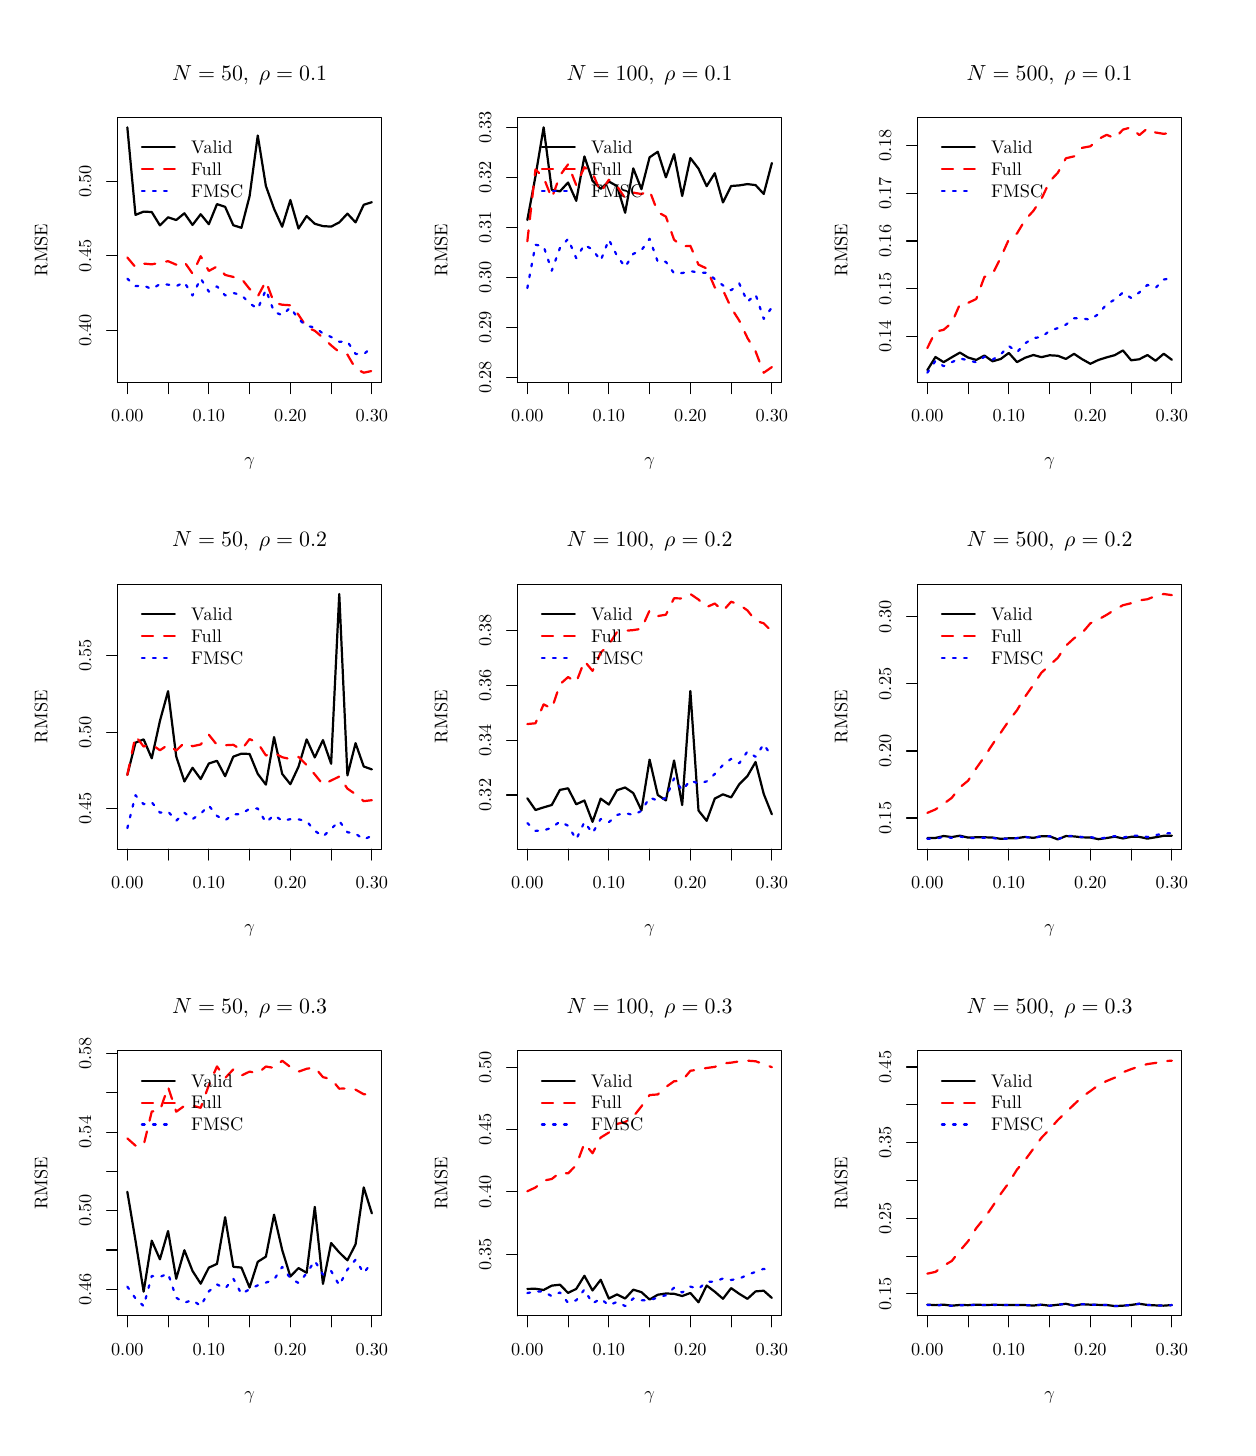
\begin{tikzpicture}[x=1pt,y=1pt]
\definecolor[named]{fillColor}{rgb}{1.00,1.00,1.00}
\path[use as bounding box,fill=fillColor,fill opacity=0.00] (0,0) rectangle (433.62,505.89);
\begin{scope}
\path[clip] ( 32.47,377.65) rectangle (127.91,473.42);
\definecolor[named]{drawColor}{rgb}{0.00,0.00,0.00}

\path[draw=drawColor,line width= 0.8pt,line join=round,line cap=round] ( 36.01,469.87) --
	( 38.95,438.24) --
	( 41.90,439.42) --
	( 44.84,439.26) --
	( 47.79,434.44) --
	( 50.73,437.37) --
	( 53.68,436.38) --
	( 56.63,438.81) --
	( 59.57,434.60) --
	( 62.52,438.47) --
	( 65.46,434.86) --
	( 68.41,442.13) --
	( 71.35,441.13) --
	( 74.30,434.49) --
	( 77.24,433.57) --
	( 80.19,445.01) --
	( 83.14,466.93) --
	( 86.08,448.67) --
	( 89.03,440.43) --
	( 91.97,433.96) --
	( 94.92,443.62) --
	( 97.86,433.31) --
	(100.81,437.81) --
	(103.75,435.02) --
	(106.70,434.18) --
	(109.65,434.00) --
	(112.59,435.51) --
	(115.54,438.69) --
	(118.48,435.52) --
	(121.43,441.89) --
	(124.37,442.82);
\end{scope}
\begin{scope}
\path[clip] (  0.00,  0.00) rectangle (433.62,505.89);
\definecolor[named]{drawColor}{rgb}{0.00,0.00,0.00}

\path[draw=drawColor,line width= 0.4pt,line join=round,line cap=round] ( 36.01,377.65) -- (124.37,377.65);

\path[draw=drawColor,line width= 0.4pt,line join=round,line cap=round] ( 36.01,377.65) -- ( 36.01,373.69);

\path[draw=drawColor,line width= 0.4pt,line join=round,line cap=round] ( 50.73,377.65) -- ( 50.73,373.69);

\path[draw=drawColor,line width= 0.4pt,line join=round,line cap=round] ( 65.46,377.65) -- ( 65.46,373.69);

\path[draw=drawColor,line width= 0.4pt,line join=round,line cap=round] ( 80.19,377.65) -- ( 80.19,373.69);

\path[draw=drawColor,line width= 0.4pt,line join=round,line cap=round] ( 94.92,377.65) -- ( 94.92,373.69);

\path[draw=drawColor,line width= 0.4pt,line join=round,line cap=round] (109.65,377.65) -- (109.65,373.69);

\path[draw=drawColor,line width= 0.4pt,line join=round,line cap=round] (124.37,377.65) -- (124.37,373.69);

\node[text=drawColor,anchor=base,inner sep=0pt, outer sep=0pt, scale=  0.66] at ( 36.01,363.40) {0.00};

\node[text=drawColor,anchor=base,inner sep=0pt, outer sep=0pt, scale=  0.66] at ( 65.46,363.40) {0.10};

\node[text=drawColor,anchor=base,inner sep=0pt, outer sep=0pt, scale=  0.66] at ( 94.92,363.40) {0.20};

\node[text=drawColor,anchor=base,inner sep=0pt, outer sep=0pt, scale=  0.66] at (124.37,363.40) {0.30};

\path[draw=drawColor,line width= 0.4pt,line join=round,line cap=round] ( 32.47,396.54) -- ( 32.47,450.39);

\path[draw=drawColor,line width= 0.4pt,line join=round,line cap=round] ( 32.47,396.54) -- ( 28.51,396.54);

\path[draw=drawColor,line width= 0.4pt,line join=round,line cap=round] ( 32.47,423.46) -- ( 28.51,423.46);

\path[draw=drawColor,line width= 0.4pt,line join=round,line cap=round] ( 32.47,450.39) -- ( 28.51,450.39);

\node[text=drawColor,rotate= 90.00,anchor=base,inner sep=0pt, outer sep=0pt, scale=  0.66] at ( 22.97,396.54) {0.40};

\node[text=drawColor,rotate= 90.00,anchor=base,inner sep=0pt, outer sep=0pt, scale=  0.66] at ( 22.97,423.46) {0.45};

\node[text=drawColor,rotate= 90.00,anchor=base,inner sep=0pt, outer sep=0pt, scale=  0.66] at ( 22.97,450.39) {0.50};

\path[draw=drawColor,line width= 0.4pt,line join=round,line cap=round] ( 32.47,377.65) --
	(127.91,377.65) --
	(127.91,473.42) --
	( 32.47,473.42) --
	( 32.47,377.65);
\end{scope}
\begin{scope}
\path[clip] (  0.00,337.26) rectangle (144.54,505.89);
\definecolor[named]{drawColor}{rgb}{0.00,0.00,0.00}

\node[text=drawColor,anchor=base,inner sep=0pt, outer sep=0pt, scale=  0.79] at ( 80.19,486.92) {\bfseries $N=50, \;\rho=0.1$};

\node[text=drawColor,anchor=base,inner sep=0pt, outer sep=0pt, scale=  0.66] at ( 80.19,347.56) {$\gamma$};

\node[text=drawColor,rotate= 90.00,anchor=base,inner sep=0pt, outer sep=0pt, scale=  0.66] at (  7.13,425.53) {RMSE};
\end{scope}
\begin{scope}
\path[clip] ( 32.47,377.65) rectangle (127.91,473.42);
\definecolor[named]{drawColor}{rgb}{1.00,0.00,0.00}

\path[draw=drawColor,line width= 0.8pt,dash pattern=on 4pt off 4pt ,line join=round,line cap=round] ( 36.01,422.84) --
	( 38.95,419.35) --
	( 41.90,420.63) --
	( 44.84,420.37) --
	( 47.79,420.92) --
	( 50.73,421.51) --
	( 53.68,420.24) --
	( 56.63,421.24) --
	( 59.57,417.02) --
	( 62.52,423.30) --
	( 65.46,417.98) --
	( 68.41,419.59) --
	( 71.35,416.53) --
	( 74.30,415.81) --
	( 77.24,415.20) --
	( 80.19,411.48) --
	( 83.14,408.77) --
	( 86.08,414.25) --
	( 89.03,406.46) --
	( 91.97,405.77) --
	( 94.92,405.57) --
	( 97.86,402.16) --
	(100.81,397.64) --
	(103.75,396.36) --
	(106.70,393.85) --
	(109.65,391.09) --
	(112.59,388.64) --
	(115.54,387.75) --
	(118.48,382.70) --
	(121.43,381.20) --
	(124.37,381.84);
\definecolor[named]{drawColor}{rgb}{0.00,0.00,1.00}

\path[draw=drawColor,line width= 0.8pt,dash pattern=on 1pt off 3pt ,line join=round,line cap=round] ( 36.01,415.20) --
	( 38.95,412.50) --
	( 41.90,412.72) --
	( 44.84,411.42) --
	( 47.79,413.23) --
	( 50.73,413.03) --
	( 53.68,412.47) --
	( 56.63,413.89) --
	( 59.57,409.12) --
	( 62.52,415.25) --
	( 65.46,410.52) --
	( 68.41,412.41) --
	( 71.35,409.14) --
	( 74.30,410.03) --
	( 77.24,409.24) --
	( 80.19,406.31) --
	( 83.14,404.27) --
	( 86.08,411.18) --
	( 89.03,403.23) --
	( 91.97,401.97) --
	( 94.92,404.78) --
	( 97.86,400.56) --
	(100.81,398.08) --
	(103.75,397.59) --
	(106.70,395.38) --
	(109.65,394.13) --
	(112.59,392.41) --
	(115.54,392.46) --
	(118.48,388.01) --
	(121.43,387.91) --
	(124.37,390.35);
\definecolor[named]{drawColor}{rgb}{0.00,0.00,0.00}

\path[draw=drawColor,line width= 0.8pt,line join=round,line cap=round] ( 41.28,462.63) -- ( 53.16,462.63);
\definecolor[named]{drawColor}{rgb}{1.00,0.00,0.00}

\path[draw=drawColor,line width= 0.8pt,dash pattern=on 4pt off 4pt ,line join=round,line cap=round] ( 41.28,454.71) -- ( 53.16,454.71);
\definecolor[named]{drawColor}{rgb}{0.00,0.00,1.00}

\path[draw=drawColor,line width= 0.8pt,dash pattern=on 1pt off 3pt ,line join=round,line cap=round] ( 41.28,446.79) -- ( 53.16,446.79);
\definecolor[named]{drawColor}{rgb}{0.00,0.00,0.00}

\node[text=drawColor,anchor=base west,inner sep=0pt, outer sep=0pt, scale=  0.66] at ( 59.10,460.35) {Valid};

\node[text=drawColor,anchor=base west,inner sep=0pt, outer sep=0pt, scale=  0.66] at ( 59.10,452.43) {Full};

\node[text=drawColor,anchor=base west,inner sep=0pt, outer sep=0pt, scale=  0.66] at ( 59.10,444.51) {FMSC};
\end{scope}
\begin{scope}
\path[clip] (177.01,377.65) rectangle (272.45,473.42);
\definecolor[named]{drawColor}{rgb}{0.00,0.00,0.00}

\path[draw=drawColor,line width= 0.8pt,line join=round,line cap=round] (180.55,436.38) --
	(183.49,452.19) --
	(186.44,469.87) --
	(189.38,447.26) --
	(192.33,446.74) --
	(195.27,449.93) --
	(198.22,443.33) --
	(201.17,459.36) --
	(204.11,450.53) --
	(207.06,447.67) --
	(210.00,450.30) --
	(212.95,448.65) --
	(215.89,439.02) --
	(218.84,455.03) --
	(221.78,447.52) --
	(224.73,459.04) --
	(227.68,461.05) --
	(230.62,451.80) --
	(233.57,460.19) --
	(236.51,445.06) --
	(239.46,458.78) --
	(242.40,454.95) --
	(245.35,448.62) --
	(248.29,453.29) --
	(251.24,442.73) --
	(254.19,448.67) --
	(257.13,448.89) --
	(260.08,449.36) --
	(263.02,449.00) --
	(265.97,445.80) --
	(268.91,456.97);
\end{scope}
\begin{scope}
\path[clip] (  0.00,  0.00) rectangle (433.62,505.89);
\definecolor[named]{drawColor}{rgb}{0.00,0.00,0.00}

\path[draw=drawColor,line width= 0.4pt,line join=round,line cap=round] (180.55,377.65) -- (268.91,377.65);

\path[draw=drawColor,line width= 0.4pt,line join=round,line cap=round] (180.55,377.65) -- (180.55,373.69);

\path[draw=drawColor,line width= 0.4pt,line join=round,line cap=round] (195.27,377.65) -- (195.27,373.69);

\path[draw=drawColor,line width= 0.4pt,line join=round,line cap=round] (210.00,377.65) -- (210.00,373.69);

\path[draw=drawColor,line width= 0.4pt,line join=round,line cap=round] (224.73,377.65) -- (224.73,373.69);

\path[draw=drawColor,line width= 0.4pt,line join=round,line cap=round] (239.46,377.65) -- (239.46,373.69);

\path[draw=drawColor,line width= 0.4pt,line join=round,line cap=round] (254.19,377.65) -- (254.19,373.69);

\path[draw=drawColor,line width= 0.4pt,line join=round,line cap=round] (268.91,377.65) -- (268.91,373.69);

\node[text=drawColor,anchor=base,inner sep=0pt, outer sep=0pt, scale=  0.66] at (180.55,363.40) {0.00};

\node[text=drawColor,anchor=base,inner sep=0pt, outer sep=0pt, scale=  0.66] at (210.00,363.40) {0.10};

\node[text=drawColor,anchor=base,inner sep=0pt, outer sep=0pt, scale=  0.66] at (239.46,363.40) {0.20};

\node[text=drawColor,anchor=base,inner sep=0pt, outer sep=0pt, scale=  0.66] at (268.91,363.40) {0.30};

\path[draw=drawColor,line width= 0.4pt,line join=round,line cap=round] (177.01,379.47) -- (177.01,469.73);

\path[draw=drawColor,line width= 0.4pt,line join=round,line cap=round] (177.01,379.47) -- (173.05,379.47);

\path[draw=drawColor,line width= 0.4pt,line join=round,line cap=round] (177.01,397.52) -- (173.05,397.52);

\path[draw=drawColor,line width= 0.4pt,line join=round,line cap=round] (177.01,415.58) -- (173.05,415.58);

\path[draw=drawColor,line width= 0.4pt,line join=round,line cap=round] (177.01,433.63) -- (173.05,433.63);

\path[draw=drawColor,line width= 0.4pt,line join=round,line cap=round] (177.01,451.68) -- (173.05,451.68);

\path[draw=drawColor,line width= 0.4pt,line join=round,line cap=round] (177.01,469.73) -- (173.05,469.73);

\node[text=drawColor,rotate= 90.00,anchor=base,inner sep=0pt, outer sep=0pt, scale=  0.66] at (167.51,379.47) {0.28};

\node[text=drawColor,rotate= 90.00,anchor=base,inner sep=0pt, outer sep=0pt, scale=  0.66] at (167.51,397.52) {0.29};

\node[text=drawColor,rotate= 90.00,anchor=base,inner sep=0pt, outer sep=0pt, scale=  0.66] at (167.51,415.58) {0.30};

\node[text=drawColor,rotate= 90.00,anchor=base,inner sep=0pt, outer sep=0pt, scale=  0.66] at (167.51,433.63) {0.31};

\node[text=drawColor,rotate= 90.00,anchor=base,inner sep=0pt, outer sep=0pt, scale=  0.66] at (167.51,451.68) {0.32};

\node[text=drawColor,rotate= 90.00,anchor=base,inner sep=0pt, outer sep=0pt, scale=  0.66] at (167.51,469.73) {0.33};

\path[draw=drawColor,line width= 0.4pt,line join=round,line cap=round] (177.01,377.65) --
	(272.45,377.65) --
	(272.45,473.42) --
	(177.01,473.42) --
	(177.01,377.65);
\end{scope}
\begin{scope}
\path[clip] (144.54,337.26) rectangle (289.08,505.89);
\definecolor[named]{drawColor}{rgb}{0.00,0.00,0.00}

\node[text=drawColor,anchor=base,inner sep=0pt, outer sep=0pt, scale=  0.79] at (224.73,486.92) {\bfseries $N=100, \;\rho=0.1$};

\node[text=drawColor,anchor=base,inner sep=0pt, outer sep=0pt, scale=  0.66] at (224.73,347.56) {$\gamma$};

\node[text=drawColor,rotate= 90.00,anchor=base,inner sep=0pt, outer sep=0pt, scale=  0.66] at (151.67,425.53) {RMSE};
\end{scope}
\begin{scope}
\path[clip] (177.01,377.65) rectangle (272.45,473.42);
\definecolor[named]{drawColor}{rgb}{1.00,0.00,0.00}

\path[draw=drawColor,line width= 0.8pt,dash pattern=on 4pt off 4pt ,line join=round,line cap=round] (180.55,428.69) --
	(183.49,454.68) --
	(186.44,451.70) --
	(189.38,444.28) --
	(192.33,452.45) --
	(195.27,456.48) --
	(198.22,449.01) --
	(201.17,455.46) --
	(204.11,453.37) --
	(207.06,446.42) --
	(210.00,450.92) --
	(212.95,448.63) --
	(215.89,444.23) --
	(218.84,446.28) --
	(221.78,445.77) --
	(224.73,446.98) --
	(227.68,439.24) --
	(230.62,437.61) --
	(233.57,429.26) --
	(236.51,426.86) --
	(239.46,427.05) --
	(242.40,420.25) --
	(245.35,418.87) --
	(248.29,412.01) --
	(251.24,411.05) --
	(254.19,404.64) --
	(257.13,400.04) --
	(260.08,393.78) --
	(263.02,388.93) --
	(265.97,381.20) --
	(268.91,383.23);
\definecolor[named]{drawColor}{rgb}{0.00,0.00,1.00}

\path[draw=drawColor,line width= 0.8pt,dash pattern=on 1pt off 3pt ,line join=round,line cap=round] (180.55,411.78) --
	(183.49,427.44) --
	(186.44,426.88) --
	(189.38,418.08) --
	(192.33,426.27) --
	(195.27,429.57) --
	(198.22,422.61) --
	(201.17,427.44) --
	(204.11,425.67) --
	(207.06,421.71) --
	(210.00,429.31) --
	(212.95,423.48) --
	(215.89,419.39) --
	(218.84,424.15) --
	(221.78,425.45) --
	(224.73,429.61) --
	(227.68,421.30) --
	(230.62,421.27) --
	(233.57,417.11) --
	(236.51,417.21) --
	(239.46,417.94) --
	(242.40,417.38) --
	(245.35,417.30) --
	(248.29,415.05) --
	(251.24,412.76) --
	(254.19,410.99) --
	(257.13,413.44) --
	(260.08,406.83) --
	(263.02,409.52) --
	(265.97,400.65) --
	(268.91,404.84);
\definecolor[named]{drawColor}{rgb}{0.00,0.00,0.00}

\path[draw=drawColor,line width= 0.8pt,line join=round,line cap=round] (185.82,462.63) -- (197.70,462.63);
\definecolor[named]{drawColor}{rgb}{1.00,0.00,0.00}

\path[draw=drawColor,line width= 0.8pt,dash pattern=on 4pt off 4pt ,line join=round,line cap=round] (185.82,454.71) -- (197.70,454.71);
\definecolor[named]{drawColor}{rgb}{0.00,0.00,1.00}

\path[draw=drawColor,line width= 0.8pt,dash pattern=on 1pt off 3pt ,line join=round,line cap=round] (185.82,446.79) -- (197.70,446.79);
\definecolor[named]{drawColor}{rgb}{0.00,0.00,0.00}

\node[text=drawColor,anchor=base west,inner sep=0pt, outer sep=0pt, scale=  0.66] at (203.64,460.35) {Valid};

\node[text=drawColor,anchor=base west,inner sep=0pt, outer sep=0pt, scale=  0.66] at (203.64,452.43) {Full};

\node[text=drawColor,anchor=base west,inner sep=0pt, outer sep=0pt, scale=  0.66] at (203.64,444.51) {FMSC};
\end{scope}
\begin{scope}
\path[clip] (321.55,377.65) rectangle (416.99,473.42);
\definecolor[named]{drawColor}{rgb}{0.00,0.00,0.00}

\path[draw=drawColor,line width= 0.8pt,line join=round,line cap=round] (325.09,382.14) --
	(328.03,386.88) --
	(330.98,385.02) --
	(333.92,386.78) --
	(336.87,388.47) --
	(339.81,386.69) --
	(342.76,385.83) --
	(345.71,387.41) --
	(348.65,385.33) --
	(351.60,386.16) --
	(354.54,388.35) --
	(357.49,385.04) --
	(360.43,386.61) --
	(363.38,387.61) --
	(366.32,386.82) --
	(369.27,387.51) --
	(372.22,387.33) --
	(375.16,386.18) --
	(378.11,388.03) --
	(381.05,386.08) --
	(384.00,384.43) --
	(386.94,385.83) --
	(389.89,386.75) --
	(392.83,387.55) --
	(395.78,389.25) --
	(398.73,385.70) --
	(401.67,386.06) --
	(404.62,387.60) --
	(407.56,385.53) --
	(410.51,388.06) --
	(413.45,385.88);
\end{scope}
\begin{scope}
\path[clip] (  0.00,  0.00) rectangle (433.62,505.89);
\definecolor[named]{drawColor}{rgb}{0.00,0.00,0.00}

\path[draw=drawColor,line width= 0.4pt,line join=round,line cap=round] (325.09,377.65) -- (413.45,377.65);

\path[draw=drawColor,line width= 0.4pt,line join=round,line cap=round] (325.09,377.65) -- (325.09,373.69);

\path[draw=drawColor,line width= 0.4pt,line join=round,line cap=round] (339.81,377.65) -- (339.81,373.69);

\path[draw=drawColor,line width= 0.4pt,line join=round,line cap=round] (354.54,377.65) -- (354.54,373.69);

\path[draw=drawColor,line width= 0.4pt,line join=round,line cap=round] (369.27,377.65) -- (369.27,373.69);

\path[draw=drawColor,line width= 0.4pt,line join=round,line cap=round] (384.00,377.65) -- (384.00,373.69);

\path[draw=drawColor,line width= 0.4pt,line join=round,line cap=round] (398.73,377.65) -- (398.73,373.69);

\path[draw=drawColor,line width= 0.4pt,line join=round,line cap=round] (413.45,377.65) -- (413.45,373.69);

\node[text=drawColor,anchor=base,inner sep=0pt, outer sep=0pt, scale=  0.66] at (325.09,363.40) {0.00};

\node[text=drawColor,anchor=base,inner sep=0pt, outer sep=0pt, scale=  0.66] at (354.54,363.40) {0.10};

\node[text=drawColor,anchor=base,inner sep=0pt, outer sep=0pt, scale=  0.66] at (384.00,363.40) {0.20};

\node[text=drawColor,anchor=base,inner sep=0pt, outer sep=0pt, scale=  0.66] at (413.45,363.40) {0.30};

\path[draw=drawColor,line width= 0.4pt,line join=round,line cap=round] (321.55,394.25) -- (321.55,463.36);

\path[draw=drawColor,line width= 0.4pt,line join=round,line cap=round] (321.55,394.25) -- (317.59,394.25);

\path[draw=drawColor,line width= 0.4pt,line join=round,line cap=round] (321.55,411.53) -- (317.59,411.53);

\path[draw=drawColor,line width= 0.4pt,line join=round,line cap=round] (321.55,428.81) -- (317.59,428.81);

\path[draw=drawColor,line width= 0.4pt,line join=round,line cap=round] (321.55,446.09) -- (317.59,446.09);

\path[draw=drawColor,line width= 0.4pt,line join=round,line cap=round] (321.55,463.36) -- (317.59,463.36);

\node[text=drawColor,rotate= 90.00,anchor=base,inner sep=0pt, outer sep=0pt, scale=  0.66] at (312.05,394.25) {0.14};

\node[text=drawColor,rotate= 90.00,anchor=base,inner sep=0pt, outer sep=0pt, scale=  0.66] at (312.05,411.53) {0.15};

\node[text=drawColor,rotate= 90.00,anchor=base,inner sep=0pt, outer sep=0pt, scale=  0.66] at (312.05,428.81) {0.16};

\node[text=drawColor,rotate= 90.00,anchor=base,inner sep=0pt, outer sep=0pt, scale=  0.66] at (312.05,446.09) {0.17};

\node[text=drawColor,rotate= 90.00,anchor=base,inner sep=0pt, outer sep=0pt, scale=  0.66] at (312.05,463.36) {0.18};

\path[draw=drawColor,line width= 0.4pt,line join=round,line cap=round] (321.55,377.65) --
	(416.99,377.65) --
	(416.99,473.42) --
	(321.55,473.42) --
	(321.55,377.65);
\end{scope}
\begin{scope}
\path[clip] (289.08,337.26) rectangle (433.62,505.89);
\definecolor[named]{drawColor}{rgb}{0.00,0.00,0.00}

\node[text=drawColor,anchor=base,inner sep=0pt, outer sep=0pt, scale=  0.79] at (369.27,486.92) {\bfseries $N=500, \;\rho=0.1$};

\node[text=drawColor,anchor=base,inner sep=0pt, outer sep=0pt, scale=  0.66] at (369.27,347.56) {$\gamma$};

\node[text=drawColor,rotate= 90.00,anchor=base,inner sep=0pt, outer sep=0pt, scale=  0.66] at (296.21,425.53) {RMSE};
\end{scope}
\begin{scope}
\path[clip] (321.55,377.65) rectangle (416.99,473.42);
\definecolor[named]{drawColor}{rgb}{1.00,0.00,0.00}

\path[draw=drawColor,line width= 0.8pt,dash pattern=on 4pt off 4pt ,line join=round,line cap=round] (325.09,390.11) --
	(328.03,396.04) --
	(330.98,396.71) --
	(333.92,399.24) --
	(336.87,405.98) --
	(339.81,406.45) --
	(342.76,407.83) --
	(345.71,415.83) --
	(348.65,416.84) --
	(351.60,422.79) --
	(354.54,429.37) --
	(357.49,431.53) --
	(360.43,436.42) --
	(363.38,439.66) --
	(366.32,443.99) --
	(369.27,450.33) --
	(372.22,453.43) --
	(375.16,458.69) --
	(378.11,459.39) --
	(381.05,462.47) --
	(384.00,463.01) --
	(386.94,465.63) --
	(389.89,467.17) --
	(392.83,465.91) --
	(395.78,469.05) --
	(398.73,469.87) --
	(401.67,467.05) --
	(404.62,469.50) --
	(407.56,468.00) --
	(410.51,467.52) --
	(413.45,467.93);
\definecolor[named]{drawColor}{rgb}{0.00,0.00,1.00}

\path[draw=drawColor,line width= 0.8pt,dash pattern=on 1pt off 3pt ,line join=round,line cap=round] (325.09,381.20) --
	(328.03,385.47) --
	(330.98,383.57) --
	(333.92,385.00) --
	(336.87,386.36) --
	(339.81,385.68) --
	(342.76,384.97) --
	(345.71,386.96) --
	(348.65,385.89) --
	(351.60,387.81) --
	(354.54,390.88) --
	(357.49,388.63) --
	(360.43,391.82) --
	(363.38,393.74) --
	(366.32,394.06) --
	(369.27,396.33) --
	(372.22,397.31) --
	(375.16,398.57) --
	(378.11,400.88) --
	(381.05,400.80) --
	(384.00,400.39) --
	(386.94,402.42) --
	(389.89,406.00) --
	(392.83,407.63) --
	(395.78,410.21) --
	(398.73,408.20) --
	(401.67,410.19) --
	(404.62,412.94) --
	(407.56,411.85) --
	(410.51,414.89) --
	(413.45,415.34);
\definecolor[named]{drawColor}{rgb}{0.00,0.00,0.00}

\path[draw=drawColor,line width= 0.8pt,line join=round,line cap=round] (330.36,462.63) -- (342.24,462.63);
\definecolor[named]{drawColor}{rgb}{1.00,0.00,0.00}

\path[draw=drawColor,line width= 0.8pt,dash pattern=on 4pt off 4pt ,line join=round,line cap=round] (330.36,454.71) -- (342.24,454.71);
\definecolor[named]{drawColor}{rgb}{0.00,0.00,1.00}

\path[draw=drawColor,line width= 0.8pt,dash pattern=on 1pt off 3pt ,line join=round,line cap=round] (330.36,446.79) -- (342.24,446.79);
\definecolor[named]{drawColor}{rgb}{0.00,0.00,0.00}

\node[text=drawColor,anchor=base west,inner sep=0pt, outer sep=0pt, scale=  0.66] at (348.18,460.35) {Valid};

\node[text=drawColor,anchor=base west,inner sep=0pt, outer sep=0pt, scale=  0.66] at (348.18,452.43) {Full};

\node[text=drawColor,anchor=base west,inner sep=0pt, outer sep=0pt, scale=  0.66] at (348.18,444.51) {FMSC};
\end{scope}
\begin{scope}
\path[clip] ( 32.47,209.02) rectangle (127.91,304.79);
\definecolor[named]{drawColor}{rgb}{0.00,0.00,0.00}

\path[draw=drawColor,line width= 0.8pt,line join=round,line cap=round] ( 36.01,235.87) --
	( 38.95,247.52) --
	( 41.90,248.72) --
	( 44.84,241.87) --
	( 47.79,255.38) --
	( 50.73,266.12) --
	( 53.68,242.55) --
	( 56.63,233.51) --
	( 59.57,238.45) --
	( 62.52,234.37) --
	( 65.46,240.00) --
	( 68.41,240.96) --
	( 71.35,235.40) --
	( 74.30,242.47) --
	( 77.24,243.56) --
	( 80.19,243.44) --
	( 83.14,236.25) --
	( 86.08,232.37) --
	( 89.03,249.54) --
	( 91.97,236.24) --
	( 94.92,232.52) --
	( 97.86,238.82) --
	(100.81,248.71) --
	(103.75,242.19) --
	(106.70,248.46) --
	(109.65,239.91) --
	(112.59,301.24) --
	(115.54,235.68) --
	(118.48,247.34) --
	(121.43,238.91) --
	(124.37,237.86);
\end{scope}
\begin{scope}
\path[clip] (  0.00,  0.00) rectangle (433.62,505.89);
\definecolor[named]{drawColor}{rgb}{0.00,0.00,0.00}

\path[draw=drawColor,line width= 0.4pt,line join=round,line cap=round] ( 36.01,209.02) -- (124.37,209.02);

\path[draw=drawColor,line width= 0.4pt,line join=round,line cap=round] ( 36.01,209.02) -- ( 36.01,205.06);

\path[draw=drawColor,line width= 0.4pt,line join=round,line cap=round] ( 50.73,209.02) -- ( 50.73,205.06);

\path[draw=drawColor,line width= 0.4pt,line join=round,line cap=round] ( 65.46,209.02) -- ( 65.46,205.06);

\path[draw=drawColor,line width= 0.4pt,line join=round,line cap=round] ( 80.19,209.02) -- ( 80.19,205.06);

\path[draw=drawColor,line width= 0.4pt,line join=round,line cap=round] ( 94.92,209.02) -- ( 94.92,205.06);

\path[draw=drawColor,line width= 0.4pt,line join=round,line cap=round] (109.65,209.02) -- (109.65,205.06);

\path[draw=drawColor,line width= 0.4pt,line join=round,line cap=round] (124.37,209.02) -- (124.37,205.06);

\node[text=drawColor,anchor=base,inner sep=0pt, outer sep=0pt, scale=  0.66] at ( 36.01,194.77) {0.00};

\node[text=drawColor,anchor=base,inner sep=0pt, outer sep=0pt, scale=  0.66] at ( 65.46,194.77) {0.10};

\node[text=drawColor,anchor=base,inner sep=0pt, outer sep=0pt, scale=  0.66] at ( 94.92,194.77) {0.20};

\node[text=drawColor,anchor=base,inner sep=0pt, outer sep=0pt, scale=  0.66] at (124.37,194.77) {0.30};

\path[draw=drawColor,line width= 0.4pt,line join=round,line cap=round] ( 32.47,223.66) -- ( 32.47,278.98);

\path[draw=drawColor,line width= 0.4pt,line join=round,line cap=round] ( 32.47,223.66) -- ( 28.51,223.66);

\path[draw=drawColor,line width= 0.4pt,line join=round,line cap=round] ( 32.47,251.32) -- ( 28.51,251.32);

\path[draw=drawColor,line width= 0.4pt,line join=round,line cap=round] ( 32.47,278.98) -- ( 28.51,278.98);

\node[text=drawColor,rotate= 90.00,anchor=base,inner sep=0pt, outer sep=0pt, scale=  0.66] at ( 22.97,223.66) {0.45};

\node[text=drawColor,rotate= 90.00,anchor=base,inner sep=0pt, outer sep=0pt, scale=  0.66] at ( 22.97,251.32) {0.50};

\node[text=drawColor,rotate= 90.00,anchor=base,inner sep=0pt, outer sep=0pt, scale=  0.66] at ( 22.97,278.98) {0.55};

\path[draw=drawColor,line width= 0.4pt,line join=round,line cap=round] ( 32.47,209.02) --
	(127.91,209.02) --
	(127.91,304.79) --
	( 32.47,304.79) --
	( 32.47,209.02);
\end{scope}
\begin{scope}
\path[clip] (  0.00,168.63) rectangle (144.54,337.26);
\definecolor[named]{drawColor}{rgb}{0.00,0.00,0.00}

\node[text=drawColor,anchor=base,inner sep=0pt, outer sep=0pt, scale=  0.79] at ( 80.19,318.29) {\bfseries $N=50, \;\rho=0.2$};

\node[text=drawColor,anchor=base,inner sep=0pt, outer sep=0pt, scale=  0.66] at ( 80.19,178.93) {$\gamma$};

\node[text=drawColor,rotate= 90.00,anchor=base,inner sep=0pt, outer sep=0pt, scale=  0.66] at (  7.13,256.90) {RMSE};
\end{scope}
\begin{scope}
\path[clip] ( 32.47,209.02) rectangle (127.91,304.79);
\definecolor[named]{drawColor}{rgb}{1.00,0.00,0.00}

\path[draw=drawColor,line width= 0.8pt,dash pattern=on 4pt off 4pt ,line join=round,line cap=round] ( 36.01,235.84) --
	( 38.95,249.97) --
	( 41.90,246.14) --
	( 44.84,246.85) --
	( 47.79,244.79) --
	( 50.73,246.76) --
	( 53.68,244.66) --
	( 56.63,247.53) --
	( 59.57,246.24) --
	( 62.52,246.87) --
	( 65.46,250.40) --
	( 68.41,246.71) --
	( 71.35,246.60) --
	( 74.30,246.75) --
	( 77.24,244.95) --
	( 80.19,248.83) --
	( 83.14,247.41) --
	( 86.08,242.90) --
	( 89.03,243.86) --
	( 91.97,242.26) --
	( 94.92,241.59) --
	( 97.86,242.39) --
	(100.81,239.43) --
	(103.75,236.05) --
	(106.70,232.37) --
	(109.65,233.84) --
	(112.59,235.29) --
	(115.54,230.90) --
	(118.48,228.91) --
	(121.43,226.39) --
	(124.37,226.74);
\definecolor[named]{drawColor}{rgb}{0.00,0.00,1.00}

\path[draw=drawColor,line width= 0.8pt,dash pattern=on 1pt off 3pt ,line join=round,line cap=round] ( 36.01,216.63) --
	( 38.95,228.53) --
	( 41.90,225.29) --
	( 44.84,226.00) --
	( 47.79,222.23) --
	( 50.73,222.63) --
	( 53.68,219.30) --
	( 56.63,222.20) --
	( 59.57,219.91) --
	( 62.52,221.88) --
	( 65.46,224.80) --
	( 68.41,221.05) --
	( 71.35,219.46) --
	( 74.30,221.59) --
	( 77.24,221.75) --
	( 80.19,223.67) --
	( 83.14,223.74) --
	( 86.08,218.69) --
	( 89.03,221.34) --
	( 91.97,219.30) --
	( 94.92,219.87) --
	( 97.86,219.83) --
	(100.81,219.14) --
	(103.75,215.69) --
	(106.70,213.60) --
	(109.65,216.32) --
	(112.59,219.23) --
	(115.54,215.17) --
	(118.48,214.64) --
	(121.43,212.57) --
	(124.37,213.85);
\definecolor[named]{drawColor}{rgb}{0.00,0.00,0.00}

\path[draw=drawColor,line width= 0.8pt,line join=round,line cap=round] ( 41.28,294.00) -- ( 53.16,294.00);
\definecolor[named]{drawColor}{rgb}{1.00,0.00,0.00}

\path[draw=drawColor,line width= 0.8pt,dash pattern=on 4pt off 4pt ,line join=round,line cap=round] ( 41.28,286.08) -- ( 53.16,286.08);
\definecolor[named]{drawColor}{rgb}{0.00,0.00,1.00}

\path[draw=drawColor,line width= 0.8pt,dash pattern=on 1pt off 3pt ,line join=round,line cap=round] ( 41.28,278.16) -- ( 53.16,278.16);
\definecolor[named]{drawColor}{rgb}{0.00,0.00,0.00}

\node[text=drawColor,anchor=base west,inner sep=0pt, outer sep=0pt, scale=  0.66] at ( 59.10,291.72) {Valid};

\node[text=drawColor,anchor=base west,inner sep=0pt, outer sep=0pt, scale=  0.66] at ( 59.10,283.80) {Full};

\node[text=drawColor,anchor=base west,inner sep=0pt, outer sep=0pt, scale=  0.66] at ( 59.10,275.88) {FMSC};
\end{scope}
\begin{scope}
\path[clip] (177.01,209.02) rectangle (272.45,304.79);
\definecolor[named]{drawColor}{rgb}{0.00,0.00,0.00}

\path[draw=drawColor,line width= 0.8pt,line join=round,line cap=round] (180.55,227.43) --
	(183.49,223.19) --
	(186.44,224.14) --
	(189.38,225.00) --
	(192.33,230.46) --
	(195.27,231.04) --
	(198.22,225.26) --
	(201.17,226.62) --
	(204.11,218.91) --
	(207.06,227.29) --
	(210.00,225.16) --
	(212.95,230.35) --
	(215.89,231.33) --
	(218.84,229.29) --
	(221.78,223.08) --
	(224.73,241.40) --
	(227.68,228.64) --
	(230.62,226.65) --
	(233.57,241.09) --
	(236.51,224.98) --
	(239.46,266.19) --
	(242.40,223.00) --
	(245.35,219.29) --
	(248.29,227.32) --
	(251.24,228.85) --
	(254.19,227.75) --
	(257.13,232.51) --
	(260.08,235.45) --
	(263.02,240.55) --
	(265.97,229.00) --
	(268.91,221.64);
\end{scope}
\begin{scope}
\path[clip] (  0.00,  0.00) rectangle (433.62,505.89);
\definecolor[named]{drawColor}{rgb}{0.00,0.00,0.00}

\path[draw=drawColor,line width= 0.4pt,line join=round,line cap=round] (180.55,209.02) -- (268.91,209.02);

\path[draw=drawColor,line width= 0.4pt,line join=round,line cap=round] (180.55,209.02) -- (180.55,205.06);

\path[draw=drawColor,line width= 0.4pt,line join=round,line cap=round] (195.27,209.02) -- (195.27,205.06);

\path[draw=drawColor,line width= 0.4pt,line join=round,line cap=round] (210.00,209.02) -- (210.00,205.06);

\path[draw=drawColor,line width= 0.4pt,line join=round,line cap=round] (224.73,209.02) -- (224.73,205.06);

\path[draw=drawColor,line width= 0.4pt,line join=round,line cap=round] (239.46,209.02) -- (239.46,205.06);

\path[draw=drawColor,line width= 0.4pt,line join=round,line cap=round] (254.19,209.02) -- (254.19,205.06);

\path[draw=drawColor,line width= 0.4pt,line join=round,line cap=round] (268.91,209.02) -- (268.91,205.06);

\node[text=drawColor,anchor=base,inner sep=0pt, outer sep=0pt, scale=  0.66] at (180.55,194.77) {0.00};

\node[text=drawColor,anchor=base,inner sep=0pt, outer sep=0pt, scale=  0.66] at (210.00,194.77) {0.10};

\node[text=drawColor,anchor=base,inner sep=0pt, outer sep=0pt, scale=  0.66] at (239.46,194.77) {0.20};

\node[text=drawColor,anchor=base,inner sep=0pt, outer sep=0pt, scale=  0.66] at (268.91,194.77) {0.30};

\path[draw=drawColor,line width= 0.4pt,line join=round,line cap=round] (177.01,228.62) -- (177.01,287.99);

\path[draw=drawColor,line width= 0.4pt,line join=round,line cap=round] (177.01,228.62) -- (173.05,228.62);

\path[draw=drawColor,line width= 0.4pt,line join=round,line cap=round] (177.01,248.41) -- (173.05,248.41);

\path[draw=drawColor,line width= 0.4pt,line join=round,line cap=round] (177.01,268.20) -- (173.05,268.20);

\path[draw=drawColor,line width= 0.4pt,line join=round,line cap=round] (177.01,287.99) -- (173.05,287.99);

\node[text=drawColor,rotate= 90.00,anchor=base,inner sep=0pt, outer sep=0pt, scale=  0.66] at (167.51,228.62) {0.32};

\node[text=drawColor,rotate= 90.00,anchor=base,inner sep=0pt, outer sep=0pt, scale=  0.66] at (167.51,248.41) {0.34};

\node[text=drawColor,rotate= 90.00,anchor=base,inner sep=0pt, outer sep=0pt, scale=  0.66] at (167.51,268.20) {0.36};

\node[text=drawColor,rotate= 90.00,anchor=base,inner sep=0pt, outer sep=0pt, scale=  0.66] at (167.51,287.99) {0.38};

\path[draw=drawColor,line width= 0.4pt,line join=round,line cap=round] (177.01,209.02) --
	(272.45,209.02) --
	(272.45,304.79) --
	(177.01,304.79) --
	(177.01,209.02);
\end{scope}
\begin{scope}
\path[clip] (144.54,168.63) rectangle (289.08,337.26);
\definecolor[named]{drawColor}{rgb}{0.00,0.00,0.00}

\node[text=drawColor,anchor=base,inner sep=0pt, outer sep=0pt, scale=  0.79] at (224.73,318.29) {\bfseries $N=100, \;\rho=0.2$};

\node[text=drawColor,anchor=base,inner sep=0pt, outer sep=0pt, scale=  0.66] at (224.73,178.93) {$\gamma$};

\node[text=drawColor,rotate= 90.00,anchor=base,inner sep=0pt, outer sep=0pt, scale=  0.66] at (151.67,256.90) {RMSE};
\end{scope}
\begin{scope}
\path[clip] (177.01,209.02) rectangle (272.45,304.79);
\definecolor[named]{drawColor}{rgb}{1.00,0.00,0.00}

\path[draw=drawColor,line width= 0.8pt,dash pattern=on 4pt off 4pt ,line join=round,line cap=round] (180.55,254.25) --
	(183.49,254.53) --
	(186.44,261.38) --
	(189.38,259.81) --
	(192.33,268.60) --
	(195.27,271.23) --
	(198.22,269.36) --
	(201.17,277.04) --
	(204.11,273.45) --
	(207.06,280.04) --
	(210.00,282.92) --
	(212.95,287.51) --
	(215.89,287.95) --
	(218.84,288.20) --
	(221.78,288.67) --
	(224.73,295.29) --
	(227.68,293.27) --
	(230.62,293.76) --
	(233.57,299.70) --
	(236.51,299.63) --
	(239.46,301.24) --
	(242.40,299.24) --
	(245.35,296.51) --
	(248.29,297.81) --
	(251.24,295.13) --
	(254.19,298.45) --
	(257.13,297.42) --
	(260.08,295.31) --
	(263.02,291.61) --
	(265.97,290.65) --
	(268.91,287.68);
\definecolor[named]{drawColor}{rgb}{0.00,0.00,1.00}

\path[draw=drawColor,line width= 0.8pt,dash pattern=on 1pt off 3pt ,line join=round,line cap=round] (180.55,218.48) --
	(183.49,215.65) --
	(186.44,215.81) --
	(189.38,216.78) --
	(192.33,219.03) --
	(195.27,217.51) --
	(198.22,212.57) --
	(201.17,218.86) --
	(204.11,214.81) --
	(207.06,219.96) --
	(210.00,218.77) --
	(212.95,221.40) --
	(215.89,222.11) --
	(218.84,221.37) --
	(221.78,222.87) --
	(224.73,227.69) --
	(227.68,226.58) --
	(230.62,227.52) --
	(233.57,234.60) --
	(236.51,230.33) --
	(239.46,233.88) --
	(242.40,232.73) --
	(245.35,233.54) --
	(248.29,236.21) --
	(251.24,239.45) --
	(254.19,241.66) --
	(257.13,240.09) --
	(260.08,244.31) --
	(263.02,242.42) --
	(265.97,246.99) --
	(268.91,242.49);
\definecolor[named]{drawColor}{rgb}{0.00,0.00,0.00}

\path[draw=drawColor,line width= 0.8pt,line join=round,line cap=round] (185.82,294.00) -- (197.70,294.00);
\definecolor[named]{drawColor}{rgb}{1.00,0.00,0.00}

\path[draw=drawColor,line width= 0.8pt,dash pattern=on 4pt off 4pt ,line join=round,line cap=round] (185.82,286.08) -- (197.70,286.08);
\definecolor[named]{drawColor}{rgb}{0.00,0.00,1.00}

\path[draw=drawColor,line width= 0.8pt,dash pattern=on 1pt off 3pt ,line join=round,line cap=round] (185.82,278.16) -- (197.70,278.16);
\definecolor[named]{drawColor}{rgb}{0.00,0.00,0.00}

\node[text=drawColor,anchor=base west,inner sep=0pt, outer sep=0pt, scale=  0.66] at (203.64,291.72) {Valid};

\node[text=drawColor,anchor=base west,inner sep=0pt, outer sep=0pt, scale=  0.66] at (203.64,283.80) {Full};

\node[text=drawColor,anchor=base west,inner sep=0pt, outer sep=0pt, scale=  0.66] at (203.64,275.88) {FMSC};
\end{scope}
\begin{scope}
\path[clip] (321.55,209.02) rectangle (416.99,304.79);
\definecolor[named]{drawColor}{rgb}{0.00,0.00,0.00}

\path[draw=drawColor,line width= 0.8pt,line join=round,line cap=round] (325.09,213.04) --
	(328.03,213.10) --
	(330.98,213.79) --
	(333.92,213.42) --
	(336.87,213.90) --
	(339.81,213.23) --
	(342.76,213.33) --
	(345.71,213.33) --
	(348.65,213.24) --
	(351.60,212.77) --
	(354.54,212.97) --
	(357.49,213.04) --
	(360.43,213.46) --
	(363.38,213.12) --
	(366.32,213.71) --
	(369.27,213.70) --
	(372.22,212.57) --
	(375.16,213.78) --
	(378.11,213.65) --
	(381.05,213.31) --
	(384.00,213.26) --
	(386.94,212.65) --
	(389.89,213.07) --
	(392.83,213.55) --
	(395.78,212.91) --
	(398.73,213.50) --
	(401.67,213.48) --
	(404.62,212.85) --
	(407.56,213.34) --
	(410.51,213.87) --
	(413.45,213.90);
\end{scope}
\begin{scope}
\path[clip] (  0.00,  0.00) rectangle (433.62,505.89);
\definecolor[named]{drawColor}{rgb}{0.00,0.00,0.00}

\path[draw=drawColor,line width= 0.4pt,line join=round,line cap=round] (325.09,209.02) -- (413.45,209.02);

\path[draw=drawColor,line width= 0.4pt,line join=round,line cap=round] (325.09,209.02) -- (325.09,205.06);

\path[draw=drawColor,line width= 0.4pt,line join=round,line cap=round] (339.81,209.02) -- (339.81,205.06);

\path[draw=drawColor,line width= 0.4pt,line join=round,line cap=round] (354.54,209.02) -- (354.54,205.06);

\path[draw=drawColor,line width= 0.4pt,line join=round,line cap=round] (369.27,209.02) -- (369.27,205.06);

\path[draw=drawColor,line width= 0.4pt,line join=round,line cap=round] (384.00,209.02) -- (384.00,205.06);

\path[draw=drawColor,line width= 0.4pt,line join=round,line cap=round] (398.73,209.02) -- (398.73,205.06);

\path[draw=drawColor,line width= 0.4pt,line join=round,line cap=round] (413.45,209.02) -- (413.45,205.06);

\node[text=drawColor,anchor=base,inner sep=0pt, outer sep=0pt, scale=  0.66] at (325.09,194.77) {0.00};

\node[text=drawColor,anchor=base,inner sep=0pt, outer sep=0pt, scale=  0.66] at (354.54,194.77) {0.10};

\node[text=drawColor,anchor=base,inner sep=0pt, outer sep=0pt, scale=  0.66] at (384.00,194.77) {0.20};

\node[text=drawColor,anchor=base,inner sep=0pt, outer sep=0pt, scale=  0.66] at (413.45,194.77) {0.30};

\path[draw=drawColor,line width= 0.4pt,line join=round,line cap=round] (321.55,220.29) -- (321.55,293.00);

\path[draw=drawColor,line width= 0.4pt,line join=round,line cap=round] (321.55,220.29) -- (317.59,220.29);

\path[draw=drawColor,line width= 0.4pt,line join=round,line cap=round] (321.55,244.53) -- (317.59,244.53);

\path[draw=drawColor,line width= 0.4pt,line join=round,line cap=round] (321.55,268.76) -- (317.59,268.76);

\path[draw=drawColor,line width= 0.4pt,line join=round,line cap=round] (321.55,293.00) -- (317.59,293.00);

\node[text=drawColor,rotate= 90.00,anchor=base,inner sep=0pt, outer sep=0pt, scale=  0.66] at (312.05,220.29) {0.15};

\node[text=drawColor,rotate= 90.00,anchor=base,inner sep=0pt, outer sep=0pt, scale=  0.66] at (312.05,244.53) {0.20};

\node[text=drawColor,rotate= 90.00,anchor=base,inner sep=0pt, outer sep=0pt, scale=  0.66] at (312.05,268.76) {0.25};

\node[text=drawColor,rotate= 90.00,anchor=base,inner sep=0pt, outer sep=0pt, scale=  0.66] at (312.05,293.00) {0.30};

\path[draw=drawColor,line width= 0.4pt,line join=round,line cap=round] (321.55,209.02) --
	(416.99,209.02) --
	(416.99,304.79) --
	(321.55,304.79) --
	(321.55,209.02);
\end{scope}
\begin{scope}
\path[clip] (289.08,168.63) rectangle (433.62,337.26);
\definecolor[named]{drawColor}{rgb}{0.00,0.00,0.00}

\node[text=drawColor,anchor=base,inner sep=0pt, outer sep=0pt, scale=  0.79] at (369.27,318.29) {\bfseries $N=500, \;\rho=0.2$};

\node[text=drawColor,anchor=base,inner sep=0pt, outer sep=0pt, scale=  0.66] at (369.27,178.93) {$\gamma$};

\node[text=drawColor,rotate= 90.00,anchor=base,inner sep=0pt, outer sep=0pt, scale=  0.66] at (296.21,256.90) {RMSE};
\end{scope}
\begin{scope}
\path[clip] (321.55,209.02) rectangle (416.99,304.79);
\definecolor[named]{drawColor}{rgb}{1.00,0.00,0.00}

\path[draw=drawColor,line width= 0.8pt,dash pattern=on 4pt off 4pt ,line join=round,line cap=round] (325.09,222.15) --
	(328.03,223.40) --
	(330.98,225.43) --
	(333.92,227.58) --
	(336.87,231.38) --
	(339.81,233.78) --
	(342.76,238.27) --
	(345.71,242.41) --
	(348.65,246.93) --
	(351.60,251.12) --
	(354.54,255.45) --
	(357.49,259.26) --
	(360.43,264.18) --
	(363.38,268.36) --
	(366.32,272.82) --
	(369.27,275.52) --
	(372.22,278.17) --
	(375.16,282.54) --
	(378.11,285.25) --
	(381.05,287.19) --
	(384.00,290.66) --
	(386.94,292.06) --
	(389.89,293.71) --
	(392.83,295.59) --
	(395.78,297.19) --
	(398.73,297.91) --
	(401.67,298.95) --
	(404.62,299.35) --
	(407.56,300.50) --
	(410.51,301.24) --
	(413.45,300.84);
\definecolor[named]{drawColor}{rgb}{0.00,0.00,1.00}

\path[draw=drawColor,line width= 0.8pt,dash pattern=on 1pt off 3pt ,line join=round,line cap=round] (325.09,212.80) --
	(328.03,212.82) --
	(330.98,213.46) --
	(333.92,213.14) --
	(336.87,213.63) --
	(339.81,213.01) --
	(342.76,213.12) --
	(345.71,213.17) --
	(348.65,213.09) --
	(351.60,212.68) --
	(354.54,212.91) --
	(357.49,213.02) --
	(360.43,213.45) --
	(363.38,213.11) --
	(366.32,213.72) --
	(369.27,213.72) --
	(372.22,212.62) --
	(375.16,213.87) --
	(378.11,213.74) --
	(381.05,213.42) --
	(384.00,213.43) --
	(386.94,212.84) --
	(389.89,213.23) --
	(392.83,213.75) --
	(395.78,213.20) --
	(398.73,213.94) --
	(401.67,213.93) --
	(404.62,213.44) --
	(407.56,214.10) --
	(410.51,214.73) --
	(413.45,214.83);
\definecolor[named]{drawColor}{rgb}{0.00,0.00,0.00}

\path[draw=drawColor,line width= 0.8pt,line join=round,line cap=round] (330.36,294.00) -- (342.24,294.00);
\definecolor[named]{drawColor}{rgb}{1.00,0.00,0.00}

\path[draw=drawColor,line width= 0.8pt,dash pattern=on 4pt off 4pt ,line join=round,line cap=round] (330.36,286.08) -- (342.24,286.08);
\definecolor[named]{drawColor}{rgb}{0.00,0.00,1.00}

\path[draw=drawColor,line width= 0.8pt,dash pattern=on 1pt off 3pt ,line join=round,line cap=round] (330.36,278.16) -- (342.24,278.16);
\definecolor[named]{drawColor}{rgb}{0.00,0.00,0.00}

\node[text=drawColor,anchor=base west,inner sep=0pt, outer sep=0pt, scale=  0.66] at (348.18,291.72) {Valid};

\node[text=drawColor,anchor=base west,inner sep=0pt, outer sep=0pt, scale=  0.66] at (348.18,283.80) {Full};

\node[text=drawColor,anchor=base west,inner sep=0pt, outer sep=0pt, scale=  0.66] at (348.18,275.88) {FMSC};
\end{scope}
\begin{scope}
\path[clip] ( 32.47, 40.39) rectangle (127.91,136.16);
\definecolor[named]{drawColor}{rgb}{0.00,0.00,0.00}

\path[draw=drawColor,line width= 0.8pt,line join=round,line cap=round] ( 36.01, 85.24) --
	( 38.95, 67.69) --
	( 41.90, 49.15) --
	( 44.84, 67.56) --
	( 47.79, 60.84) --
	( 50.73, 71.05) --
	( 53.68, 53.80) --
	( 56.63, 64.12) --
	( 59.57, 56.62) --
	( 62.52, 52.04) --
	( 65.46, 57.83) --
	( 68.41, 59.18) --
	( 71.35, 76.06) --
	( 74.30, 58.14) --
	( 77.24, 57.85) --
	( 80.19, 50.65) --
	( 83.14, 59.93) --
	( 86.08, 61.80) --
	( 89.03, 76.96) --
	( 91.97, 64.20) --
	( 94.92, 54.62) --
	( 97.86, 57.67) --
	(100.81, 55.97) --
	(103.75, 79.79) --
	(106.70, 51.95) --
	(109.65, 66.72) --
	(112.59, 63.32) --
	(115.54, 60.47) --
	(118.48, 66.28) --
	(121.43, 86.83) --
	(124.37, 77.43);
\end{scope}
\begin{scope}
\path[clip] (  0.00,  0.00) rectangle (433.62,505.89);
\definecolor[named]{drawColor}{rgb}{0.00,0.00,0.00}

\path[draw=drawColor,line width= 0.4pt,line join=round,line cap=round] ( 36.01, 40.39) -- (124.37, 40.39);

\path[draw=drawColor,line width= 0.4pt,line join=round,line cap=round] ( 36.01, 40.39) -- ( 36.01, 36.43);

\path[draw=drawColor,line width= 0.4pt,line join=round,line cap=round] ( 50.73, 40.39) -- ( 50.73, 36.43);

\path[draw=drawColor,line width= 0.4pt,line join=round,line cap=round] ( 65.46, 40.39) -- ( 65.46, 36.43);

\path[draw=drawColor,line width= 0.4pt,line join=round,line cap=round] ( 80.19, 40.39) -- ( 80.19, 36.43);

\path[draw=drawColor,line width= 0.4pt,line join=round,line cap=round] ( 94.92, 40.39) -- ( 94.92, 36.43);

\path[draw=drawColor,line width= 0.4pt,line join=round,line cap=round] (109.65, 40.39) -- (109.65, 36.43);

\path[draw=drawColor,line width= 0.4pt,line join=round,line cap=round] (124.37, 40.39) -- (124.37, 36.43);

\node[text=drawColor,anchor=base,inner sep=0pt, outer sep=0pt, scale=  0.66] at ( 36.01, 26.14) {0.00};

\node[text=drawColor,anchor=base,inner sep=0pt, outer sep=0pt, scale=  0.66] at ( 65.46, 26.14) {0.10};

\node[text=drawColor,anchor=base,inner sep=0pt, outer sep=0pt, scale=  0.66] at ( 94.92, 26.14) {0.20};

\node[text=drawColor,anchor=base,inner sep=0pt, outer sep=0pt, scale=  0.66] at (124.37, 26.14) {0.30};

\path[draw=drawColor,line width= 0.4pt,line join=round,line cap=round] ( 32.47, 49.99) -- ( 32.47,135.22);

\path[draw=drawColor,line width= 0.4pt,line join=round,line cap=round] ( 32.47, 49.99) -- ( 28.51, 49.99);

\path[draw=drawColor,line width= 0.4pt,line join=round,line cap=round] ( 32.47, 64.20) -- ( 28.51, 64.20);

\path[draw=drawColor,line width= 0.4pt,line join=round,line cap=round] ( 32.47, 78.40) -- ( 28.51, 78.40);

\path[draw=drawColor,line width= 0.4pt,line join=round,line cap=round] ( 32.47, 92.61) -- ( 28.51, 92.61);

\path[draw=drawColor,line width= 0.4pt,line join=round,line cap=round] ( 32.47,106.81) -- ( 28.51,106.81);

\path[draw=drawColor,line width= 0.4pt,line join=round,line cap=round] ( 32.47,121.02) -- ( 28.51,121.02);

\path[draw=drawColor,line width= 0.4pt,line join=round,line cap=round] ( 32.47,135.22) -- ( 28.51,135.22);

\node[text=drawColor,rotate= 90.00,anchor=base,inner sep=0pt, outer sep=0pt, scale=  0.66] at ( 22.97, 49.99) {0.46};

\node[text=drawColor,rotate= 90.00,anchor=base,inner sep=0pt, outer sep=0pt, scale=  0.66] at ( 22.97, 78.40) {0.50};

\node[text=drawColor,rotate= 90.00,anchor=base,inner sep=0pt, outer sep=0pt, scale=  0.66] at ( 22.97,106.81) {0.54};

\node[text=drawColor,rotate= 90.00,anchor=base,inner sep=0pt, outer sep=0pt, scale=  0.66] at ( 22.97,135.22) {0.58};

\path[draw=drawColor,line width= 0.4pt,line join=round,line cap=round] ( 32.47, 40.39) --
	(127.91, 40.39) --
	(127.91,136.16) --
	( 32.47,136.16) --
	( 32.47, 40.39);
\end{scope}
\begin{scope}
\path[clip] (  0.00,  0.00) rectangle (144.54,168.63);
\definecolor[named]{drawColor}{rgb}{0.00,0.00,0.00}

\node[text=drawColor,anchor=base,inner sep=0pt, outer sep=0pt, scale=  0.79] at ( 80.19,149.66) {\bfseries $N=50, \;\rho=0.3$};

\node[text=drawColor,anchor=base,inner sep=0pt, outer sep=0pt, scale=  0.66] at ( 80.19, 10.30) {$\gamma$};

\node[text=drawColor,rotate= 90.00,anchor=base,inner sep=0pt, outer sep=0pt, scale=  0.66] at (  7.13, 88.27) {RMSE};
\end{scope}
\begin{scope}
\path[clip] ( 32.47, 40.39) rectangle (127.91,136.16);
\definecolor[named]{drawColor}{rgb}{1.00,0.00,0.00}

\path[draw=drawColor,line width= 0.8pt,dash pattern=on 4pt off 4pt ,line join=round,line cap=round] ( 36.01,104.54) --
	( 38.95,101.93) --
	( 41.90,102.06) --
	( 44.84,114.25) --
	( 47.79,114.59) --
	( 50.73,123.12) --
	( 53.68,114.17) --
	( 56.63,116.29) --
	( 59.57,116.38) --
	( 62.52,115.57) --
	( 65.46,123.76) --
	( 68.41,130.54) --
	( 71.35,126.32) --
	( 74.30,129.47) --
	( 77.24,127.25) --
	( 80.19,128.66) --
	( 83.14,128.06) --
	( 86.08,130.50) --
	( 89.03,129.99) --
	( 91.97,132.61) --
	( 94.92,130.30) --
	( 97.86,128.64) --
	(100.81,129.69) --
	(103.75,130.17) --
	(106.70,126.66) --
	(109.65,125.96) --
	(112.59,122.50) --
	(115.54,122.58) --
	(118.48,122.14) --
	(121.43,120.48) --
	(124.37,120.57);
\definecolor[named]{drawColor}{rgb}{0.00,0.00,1.00}

\path[draw=drawColor,line width= 0.8pt,dash pattern=on 1pt off 3pt ,line join=round,line cap=round] ( 36.01, 50.96) --
	( 38.95, 46.72) --
	( 41.90, 43.94) --
	( 44.84, 54.82) --
	( 47.79, 54.46) --
	( 50.73, 55.71) --
	( 53.68, 46.95) --
	( 56.63, 45.17) --
	( 59.57, 46.11) --
	( 62.52, 43.96) --
	( 65.46, 49.25) --
	( 68.41, 51.75) --
	( 71.35, 50.26) --
	( 74.30, 53.86) --
	( 77.24, 48.29) --
	( 80.19, 50.05) --
	( 83.14, 51.43) --
	( 86.08, 52.41) --
	( 89.03, 53.49) --
	( 91.97, 58.09) --
	( 94.92, 53.99) --
	( 97.86, 52.28) --
	(100.81, 55.80) --
	(103.75, 60.29) --
	(106.70, 55.33) --
	(109.65, 56.62) --
	(112.59, 51.44) --
	(115.54, 57.14) --
	(118.48, 60.70) --
	(121.43, 55.86) --
	(124.37, 59.79);
\definecolor[named]{drawColor}{rgb}{0.00,0.00,0.00}

\path[draw=drawColor,line width= 0.8pt,line join=round,line cap=round] ( 41.28,125.37) -- ( 53.16,125.37);
\definecolor[named]{drawColor}{rgb}{1.00,0.00,0.00}

\path[draw=drawColor,line width= 0.8pt,dash pattern=on 4pt off 4pt ,line join=round,line cap=round] ( 41.28,117.45) -- ( 53.16,117.45);
\definecolor[named]{drawColor}{rgb}{0.00,0.00,1.00}

\path[draw=drawColor,line width= 0.8pt,dash pattern=on 1pt off 3pt ,line join=round,line cap=round] ( 41.28,109.53) -- ( 53.16,109.53);
\definecolor[named]{drawColor}{rgb}{0.00,0.00,0.00}

\node[text=drawColor,anchor=base west,inner sep=0pt, outer sep=0pt, scale=  0.66] at ( 59.10,123.09) {Valid};

\node[text=drawColor,anchor=base west,inner sep=0pt, outer sep=0pt, scale=  0.66] at ( 59.10,115.17) {Full};

\node[text=drawColor,anchor=base west,inner sep=0pt, outer sep=0pt, scale=  0.66] at ( 59.10,107.25) {FMSC};
\end{scope}
\begin{scope}
\path[clip] (177.01, 40.39) rectangle (272.45,136.16);
\definecolor[named]{drawColor}{rgb}{0.00,0.00,0.00}

\path[draw=drawColor,line width= 0.8pt,line join=round,line cap=round] (180.55, 50.14) --
	(183.49, 50.19) --
	(186.44, 49.76) --
	(189.38, 51.33) --
	(192.33, 51.65) --
	(195.27, 48.70) --
	(198.22, 50.14) --
	(201.17, 54.88) --
	(204.11, 49.57) --
	(207.06, 53.44) --
	(210.00, 46.66) --
	(212.95, 48.15) --
	(215.89, 46.67) --
	(218.84, 49.87) --
	(221.78, 48.97) --
	(224.73, 46.31) --
	(227.68, 48.04) --
	(230.62, 48.48) --
	(233.57, 48.38) --
	(236.51, 47.57) --
	(239.46, 48.67) --
	(242.40, 45.31) --
	(245.35, 51.37) --
	(248.29, 49.13) --
	(251.24, 46.58) --
	(254.19, 50.42) --
	(257.13, 48.37) --
	(260.08, 46.55) --
	(263.02, 49.24) --
	(265.97, 49.49) --
	(268.91, 46.88);
\end{scope}
\begin{scope}
\path[clip] (  0.00,  0.00) rectangle (433.62,505.89);
\definecolor[named]{drawColor}{rgb}{0.00,0.00,0.00}

\path[draw=drawColor,line width= 0.4pt,line join=round,line cap=round] (180.55, 40.39) -- (268.91, 40.39);

\path[draw=drawColor,line width= 0.4pt,line join=round,line cap=round] (180.55, 40.39) -- (180.55, 36.43);

\path[draw=drawColor,line width= 0.4pt,line join=round,line cap=round] (195.27, 40.39) -- (195.27, 36.43);

\path[draw=drawColor,line width= 0.4pt,line join=round,line cap=round] (210.00, 40.39) -- (210.00, 36.43);

\path[draw=drawColor,line width= 0.4pt,line join=round,line cap=round] (224.73, 40.39) -- (224.73, 36.43);

\path[draw=drawColor,line width= 0.4pt,line join=round,line cap=round] (239.46, 40.39) -- (239.46, 36.43);

\path[draw=drawColor,line width= 0.4pt,line join=round,line cap=round] (254.19, 40.39) -- (254.19, 36.43);

\path[draw=drawColor,line width= 0.4pt,line join=round,line cap=round] (268.91, 40.39) -- (268.91, 36.43);

\node[text=drawColor,anchor=base,inner sep=0pt, outer sep=0pt, scale=  0.66] at (180.55, 26.14) {0.00};

\node[text=drawColor,anchor=base,inner sep=0pt, outer sep=0pt, scale=  0.66] at (210.00, 26.14) {0.10};

\node[text=drawColor,anchor=base,inner sep=0pt, outer sep=0pt, scale=  0.66] at (239.46, 26.14) {0.20};

\node[text=drawColor,anchor=base,inner sep=0pt, outer sep=0pt, scale=  0.66] at (268.91, 26.14) {0.30};

\path[draw=drawColor,line width= 0.4pt,line join=round,line cap=round] (177.01, 62.65) -- (177.01,130.23);

\path[draw=drawColor,line width= 0.4pt,line join=round,line cap=round] (177.01, 62.65) -- (173.05, 62.65);

\path[draw=drawColor,line width= 0.4pt,line join=round,line cap=round] (177.01, 85.18) -- (173.05, 85.18);

\path[draw=drawColor,line width= 0.4pt,line join=round,line cap=round] (177.01,107.70) -- (173.05,107.70);

\path[draw=drawColor,line width= 0.4pt,line join=round,line cap=round] (177.01,130.23) -- (173.05,130.23);

\node[text=drawColor,rotate= 90.00,anchor=base,inner sep=0pt, outer sep=0pt, scale=  0.66] at (167.51, 62.65) {0.35};

\node[text=drawColor,rotate= 90.00,anchor=base,inner sep=0pt, outer sep=0pt, scale=  0.66] at (167.51, 85.18) {0.40};

\node[text=drawColor,rotate= 90.00,anchor=base,inner sep=0pt, outer sep=0pt, scale=  0.66] at (167.51,107.70) {0.45};

\node[text=drawColor,rotate= 90.00,anchor=base,inner sep=0pt, outer sep=0pt, scale=  0.66] at (167.51,130.23) {0.50};

\path[draw=drawColor,line width= 0.4pt,line join=round,line cap=round] (177.01, 40.39) --
	(272.45, 40.39) --
	(272.45,136.16) --
	(177.01,136.16) --
	(177.01, 40.39);
\end{scope}
\begin{scope}
\path[clip] (144.54,  0.00) rectangle (289.08,168.63);
\definecolor[named]{drawColor}{rgb}{0.00,0.00,0.00}

\node[text=drawColor,anchor=base,inner sep=0pt, outer sep=0pt, scale=  0.79] at (224.73,149.66) {\bfseries $N=100, \;\rho=0.3$};

\node[text=drawColor,anchor=base,inner sep=0pt, outer sep=0pt, scale=  0.66] at (224.73, 10.30) {$\gamma$};

\node[text=drawColor,rotate= 90.00,anchor=base,inner sep=0pt, outer sep=0pt, scale=  0.66] at (151.67, 88.27) {RMSE};
\end{scope}
\begin{scope}
\path[clip] (177.01, 40.39) rectangle (272.45,136.16);
\definecolor[named]{drawColor}{rgb}{1.00,0.00,0.00}

\path[draw=drawColor,line width= 0.8pt,dash pattern=on 4pt off 4pt ,line join=round,line cap=round] (180.55, 85.42) --
	(183.49, 86.79) --
	(186.44, 89.28) --
	(189.38, 89.86) --
	(192.33, 92.17) --
	(195.27, 91.89) --
	(198.22, 94.85) --
	(201.17,102.75) --
	(204.11, 99.17) --
	(207.06,104.83) --
	(210.00,106.65) --
	(212.95,109.77) --
	(215.89,110.41) --
	(218.84,112.40) --
	(221.78,116.10) --
	(224.73,120.19) --
	(227.68,120.41) --
	(230.62,123.08) --
	(233.57,125.18) --
	(236.51,125.39) --
	(239.46,128.96) --
	(242.40,129.41) --
	(245.35,129.97) --
	(248.29,130.37) --
	(251.24,131.62) --
	(254.19,131.90) --
	(257.13,132.36) --
	(260.08,132.61) --
	(263.02,132.40) --
	(265.97,131.40) --
	(268.91,130.25);
\definecolor[named]{drawColor}{rgb}{0.00,0.00,1.00}

\path[draw=drawColor,line width= 0.8pt,dash pattern=on 1pt off 3pt ,line join=round,line cap=round] (180.55, 48.63) --
	(183.49, 49.24) --
	(186.44, 49.17) --
	(189.38, 47.51) --
	(192.33, 48.86) --
	(195.27, 45.10) --
	(198.22, 46.03) --
	(201.17, 49.92) --
	(204.11, 44.90) --
	(207.06, 46.60) --
	(210.00, 44.23) --
	(212.95, 45.44) --
	(215.89, 43.94) --
	(218.84, 46.69) --
	(221.78, 46.04) --
	(224.73, 46.00) --
	(227.68, 47.08) --
	(230.62, 47.86) --
	(233.57, 50.58) --
	(236.51, 48.83) --
	(239.46, 50.98) --
	(242.40, 50.17) --
	(245.35, 52.73) --
	(248.29, 52.78) --
	(251.24, 53.92) --
	(254.19, 53.38) --
	(257.13, 53.85) --
	(260.08, 55.22) --
	(263.02, 56.31) --
	(265.97, 57.41) --
	(268.91, 55.79);
\definecolor[named]{drawColor}{rgb}{0.00,0.00,0.00}

\path[draw=drawColor,line width= 0.8pt,line join=round,line cap=round] (185.82,125.37) -- (197.70,125.37);
\definecolor[named]{drawColor}{rgb}{1.00,0.00,0.00}

\path[draw=drawColor,line width= 0.8pt,dash pattern=on 4pt off 4pt ,line join=round,line cap=round] (185.82,117.45) -- (197.70,117.45);
\definecolor[named]{drawColor}{rgb}{0.00,0.00,1.00}

\path[draw=drawColor,line width= 0.8pt,dash pattern=on 1pt off 3pt ,line join=round,line cap=round] (185.82,109.53) -- (197.70,109.53);
\definecolor[named]{drawColor}{rgb}{0.00,0.00,0.00}

\node[text=drawColor,anchor=base west,inner sep=0pt, outer sep=0pt, scale=  0.66] at (203.64,123.09) {Valid};

\node[text=drawColor,anchor=base west,inner sep=0pt, outer sep=0pt, scale=  0.66] at (203.64,115.17) {Full};

\node[text=drawColor,anchor=base west,inner sep=0pt, outer sep=0pt, scale=  0.66] at (203.64,107.25) {FMSC};
\end{scope}
\begin{scope}
\path[clip] (321.55, 40.39) rectangle (416.99,136.16);
\definecolor[named]{drawColor}{rgb}{0.00,0.00,0.00}

\path[draw=drawColor,line width= 0.8pt,line join=round,line cap=round] (325.09, 44.45) --
	(328.03, 44.28) --
	(330.98, 44.45) --
	(333.92, 44.09) --
	(336.87, 44.33) --
	(339.81, 44.27) --
	(342.76, 44.46) --
	(345.71, 44.32) --
	(348.65, 44.39) --
	(351.60, 44.37) --
	(354.54, 44.34) --
	(357.49, 44.29) --
	(360.43, 44.30) --
	(363.38, 44.13) --
	(366.32, 44.44) --
	(369.27, 44.08) --
	(372.22, 44.41) --
	(375.16, 44.76) --
	(378.11, 44.10) --
	(381.05, 44.60) --
	(384.00, 44.44) --
	(386.94, 44.37) --
	(389.89, 44.33) --
	(392.83, 43.94) --
	(395.78, 44.08) --
	(398.73, 44.35) --
	(401.67, 44.77) --
	(404.62, 44.34) --
	(407.56, 44.19) --
	(410.51, 44.09) --
	(413.45, 44.30);
\end{scope}
\begin{scope}
\path[clip] (  0.00,  0.00) rectangle (433.62,505.89);
\definecolor[named]{drawColor}{rgb}{0.00,0.00,0.00}

\path[draw=drawColor,line width= 0.4pt,line join=round,line cap=round] (325.09, 40.39) -- (413.45, 40.39);

\path[draw=drawColor,line width= 0.4pt,line join=round,line cap=round] (325.09, 40.39) -- (325.09, 36.43);

\path[draw=drawColor,line width= 0.4pt,line join=round,line cap=round] (339.81, 40.39) -- (339.81, 36.43);

\path[draw=drawColor,line width= 0.4pt,line join=round,line cap=round] (354.54, 40.39) -- (354.54, 36.43);

\path[draw=drawColor,line width= 0.4pt,line join=round,line cap=round] (369.27, 40.39) -- (369.27, 36.43);

\path[draw=drawColor,line width= 0.4pt,line join=round,line cap=round] (384.00, 40.39) -- (384.00, 36.43);

\path[draw=drawColor,line width= 0.4pt,line join=round,line cap=round] (398.73, 40.39) -- (398.73, 36.43);

\path[draw=drawColor,line width= 0.4pt,line join=round,line cap=round] (413.45, 40.39) -- (413.45, 36.43);

\node[text=drawColor,anchor=base,inner sep=0pt, outer sep=0pt, scale=  0.66] at (325.09, 26.14) {0.00};

\node[text=drawColor,anchor=base,inner sep=0pt, outer sep=0pt, scale=  0.66] at (354.54, 26.14) {0.10};

\node[text=drawColor,anchor=base,inner sep=0pt, outer sep=0pt, scale=  0.66] at (384.00, 26.14) {0.20};

\node[text=drawColor,anchor=base,inner sep=0pt, outer sep=0pt, scale=  0.66] at (413.45, 26.14) {0.30};

\path[draw=drawColor,line width= 0.4pt,line join=round,line cap=round] (321.55, 48.33) -- (321.55,130.32);

\path[draw=drawColor,line width= 0.4pt,line join=round,line cap=round] (321.55, 48.33) -- (317.59, 48.33);

\path[draw=drawColor,line width= 0.4pt,line join=round,line cap=round] (321.55, 61.99) -- (317.59, 61.99);

\path[draw=drawColor,line width= 0.4pt,line join=round,line cap=round] (321.55, 75.66) -- (317.59, 75.66);

\path[draw=drawColor,line width= 0.4pt,line join=round,line cap=round] (321.55, 89.32) -- (317.59, 89.32);

\path[draw=drawColor,line width= 0.4pt,line join=round,line cap=round] (321.55,102.99) -- (317.59,102.99);

\path[draw=drawColor,line width= 0.4pt,line join=round,line cap=round] (321.55,116.65) -- (317.59,116.65);

\path[draw=drawColor,line width= 0.4pt,line join=round,line cap=round] (321.55,130.32) -- (317.59,130.32);

\node[text=drawColor,rotate= 90.00,anchor=base,inner sep=0pt, outer sep=0pt, scale=  0.66] at (312.05, 48.33) {0.15};

\node[text=drawColor,rotate= 90.00,anchor=base,inner sep=0pt, outer sep=0pt, scale=  0.66] at (312.05, 75.66) {0.25};

\node[text=drawColor,rotate= 90.00,anchor=base,inner sep=0pt, outer sep=0pt, scale=  0.66] at (312.05,102.99) {0.35};

\node[text=drawColor,rotate= 90.00,anchor=base,inner sep=0pt, outer sep=0pt, scale=  0.66] at (312.05,130.32) {0.45};

\path[draw=drawColor,line width= 0.4pt,line join=round,line cap=round] (321.55, 40.39) --
	(416.99, 40.39) --
	(416.99,136.16) --
	(321.55,136.16) --
	(321.55, 40.39);
\end{scope}
\begin{scope}
\path[clip] (289.08,  0.00) rectangle (433.62,168.63);
\definecolor[named]{drawColor}{rgb}{0.00,0.00,0.00}

\node[text=drawColor,anchor=base,inner sep=0pt, outer sep=0pt, scale=  0.79] at (369.27,149.66) {\bfseries $N=500, \;\rho=0.3$};

\node[text=drawColor,anchor=base,inner sep=0pt, outer sep=0pt, scale=  0.66] at (369.27, 10.30) {$\gamma$};

\node[text=drawColor,rotate= 90.00,anchor=base,inner sep=0pt, outer sep=0pt, scale=  0.66] at (296.21, 88.27) {RMSE};
\end{scope}
\begin{scope}
\path[clip] (321.55, 40.39) rectangle (416.99,136.16);
\definecolor[named]{drawColor}{rgb}{1.00,0.00,0.00}

\path[draw=drawColor,line width= 0.8pt,dash pattern=on 4pt off 4pt ,line join=round,line cap=round] (325.09, 55.66) --
	(328.03, 56.29) --
	(330.98, 58.51) --
	(333.92, 60.24) --
	(336.87, 63.95) --
	(339.81, 67.37) --
	(342.76, 72.09) --
	(345.71, 75.73) --
	(348.65, 79.95) --
	(351.60, 84.47) --
	(354.54, 88.50) --
	(357.49, 93.27) --
	(360.43, 96.73) --
	(363.38,100.76) --
	(366.32,104.75) --
	(369.27,107.82) --
	(372.22,111.14) --
	(375.16,113.97) --
	(378.11,116.79) --
	(381.05,119.57) --
	(384.00,121.62) --
	(386.94,123.79) --
	(389.89,125.26) --
	(392.83,126.48) --
	(395.78,128.42) --
	(398.73,129.54) --
	(401.67,130.57) --
	(404.62,131.38) --
	(407.56,131.80) --
	(410.51,132.43) --
	(413.45,132.61);
\definecolor[named]{drawColor}{rgb}{0.00,0.00,1.00}

\path[draw=drawColor,line width= 0.8pt,dash pattern=on 1pt off 3pt ,line join=round,line cap=round] (325.09, 44.37) --
	(328.03, 44.17) --
	(330.98, 44.35) --
	(333.92, 44.01) --
	(336.87, 44.24) --
	(339.81, 44.21) --
	(342.76, 44.42) --
	(345.71, 44.29) --
	(348.65, 44.35) --
	(351.60, 44.36) --
	(354.54, 44.34) --
	(357.49, 44.28) --
	(360.43, 44.30) --
	(363.38, 44.12) --
	(366.32, 44.44) --
	(369.27, 44.07) --
	(372.22, 44.41) --
	(375.16, 44.76) --
	(378.11, 44.10) --
	(381.05, 44.60) --
	(384.00, 44.44) --
	(386.94, 44.37) --
	(389.89, 44.33) --
	(392.83, 43.94) --
	(395.78, 44.08) --
	(398.73, 44.35) --
	(401.67, 44.77) --
	(404.62, 44.34) --
	(407.56, 44.19) --
	(410.51, 44.09) --
	(413.45, 44.30);
\definecolor[named]{drawColor}{rgb}{0.00,0.00,0.00}

\path[draw=drawColor,line width= 0.8pt,line join=round,line cap=round] (330.36,125.37) -- (342.24,125.37);
\definecolor[named]{drawColor}{rgb}{1.00,0.00,0.00}

\path[draw=drawColor,line width= 0.8pt,dash pattern=on 4pt off 4pt ,line join=round,line cap=round] (330.36,117.45) -- (342.24,117.45);
\definecolor[named]{drawColor}{rgb}{0.00,0.00,1.00}

\path[draw=drawColor,line width= 0.8pt,dash pattern=on 1pt off 3pt ,line join=round,line cap=round] (330.36,109.53) -- (342.24,109.53);
\definecolor[named]{drawColor}{rgb}{0.00,0.00,0.00}

\node[text=drawColor,anchor=base west,inner sep=0pt, outer sep=0pt, scale=  0.66] at (348.18,123.09) {Valid};

\node[text=drawColor,anchor=base west,inner sep=0pt, outer sep=0pt, scale=  0.66] at (348.18,115.17) {Full};

\node[text=drawColor,anchor=base west,inner sep=0pt, outer sep=0pt, scale=  0.66] at (348.18,107.25) {FMSC};
\end{scope}
\end{tikzpicture}

	\caption{Caption goes here.}
\end{figure}

\begin{figure}
\centering
	% Created by tikzDevice version 0.7.0 on 2014-07-29 12:43:57
% !TEX encoding = UTF-8 Unicode
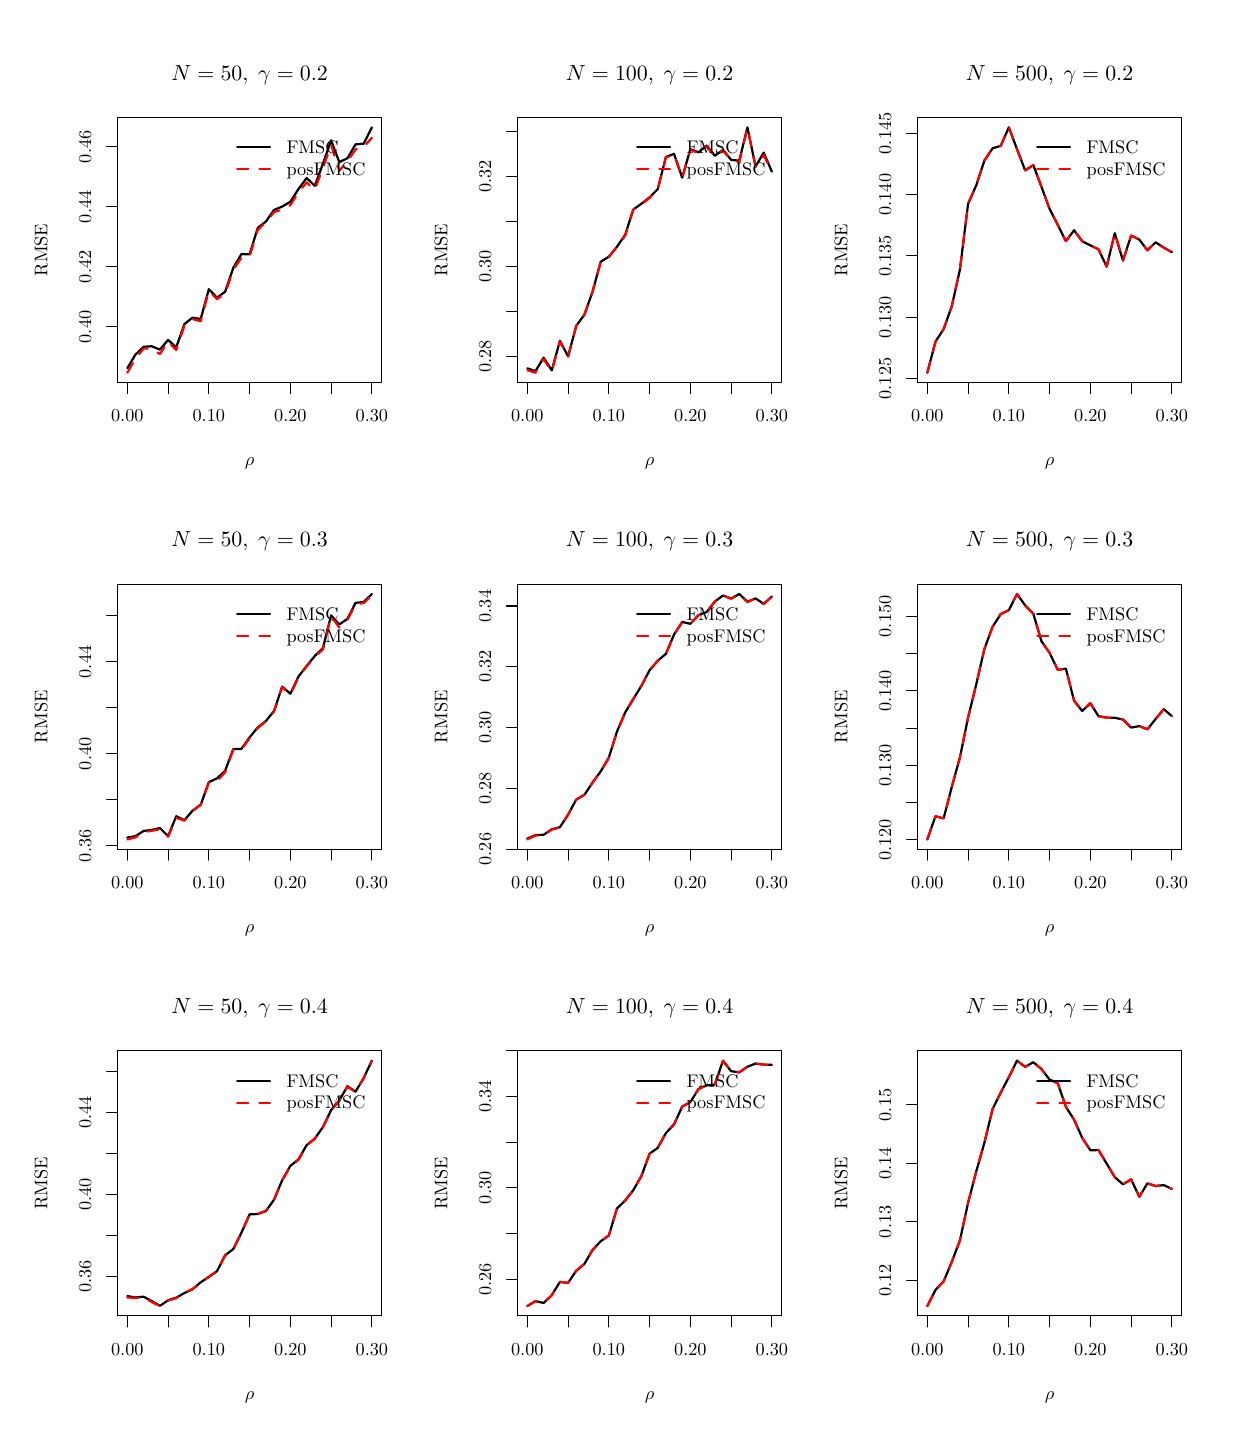
\begin{tikzpicture}[x=1pt,y=1pt]
\definecolor[named]{fillColor}{rgb}{1.00,1.00,1.00}
\path[use as bounding box,fill=fillColor,fill opacity=0.00] (0,0) rectangle (433.62,505.89);
\begin{scope}
\path[clip] ( 32.47,377.65) rectangle (127.91,473.42);
\definecolor[named]{drawColor}{rgb}{0.00,0.00,0.00}

\path[draw=drawColor,line width= 0.8pt,line join=round,line cap=round] ( 36.01,382.83) --
	( 38.95,387.77) --
	( 41.90,390.58) --
	( 44.84,390.76) --
	( 47.79,389.54) --
	( 50.73,393.05) --
	( 53.68,390.37) --
	( 56.63,398.76) --
	( 59.57,401.11) --
	( 62.52,400.61) --
	( 65.46,411.39) --
	( 68.41,408.34) --
	( 71.35,410.47) --
	( 74.30,419.12) --
	( 77.24,424.08) --
	( 80.19,423.97) --
	( 83.14,433.52) --
	( 86.08,435.83) --
	( 89.03,440.02) --
	( 91.97,441.24) --
	( 94.92,442.98) --
	( 97.86,447.59) --
	(100.81,451.55) --
	(103.75,448.74) --
	(106.70,456.75) --
	(109.65,465.17) --
	(112.59,457.33) --
	(115.54,458.69) --
	(118.48,463.72) --
	(121.43,463.97) --
	(124.37,469.87);
\end{scope}
\begin{scope}
\path[clip] (  0.00,  0.00) rectangle (433.62,505.89);
\definecolor[named]{drawColor}{rgb}{0.00,0.00,0.00}

\path[draw=drawColor,line width= 0.4pt,line join=round,line cap=round] ( 36.01,377.65) -- (124.37,377.65);

\path[draw=drawColor,line width= 0.4pt,line join=round,line cap=round] ( 36.01,377.65) -- ( 36.01,373.69);

\path[draw=drawColor,line width= 0.4pt,line join=round,line cap=round] ( 50.73,377.65) -- ( 50.73,373.69);

\path[draw=drawColor,line width= 0.4pt,line join=round,line cap=round] ( 65.46,377.65) -- ( 65.46,373.69);

\path[draw=drawColor,line width= 0.4pt,line join=round,line cap=round] ( 80.19,377.65) -- ( 80.19,373.69);

\path[draw=drawColor,line width= 0.4pt,line join=round,line cap=round] ( 94.92,377.65) -- ( 94.92,373.69);

\path[draw=drawColor,line width= 0.4pt,line join=round,line cap=round] (109.65,377.65) -- (109.65,373.69);

\path[draw=drawColor,line width= 0.4pt,line join=round,line cap=round] (124.37,377.65) -- (124.37,373.69);

\node[text=drawColor,anchor=base,inner sep=0pt, outer sep=0pt, scale=  0.66] at ( 36.01,363.40) {0.00};

\node[text=drawColor,anchor=base,inner sep=0pt, outer sep=0pt, scale=  0.66] at ( 65.46,363.40) {0.10};

\node[text=drawColor,anchor=base,inner sep=0pt, outer sep=0pt, scale=  0.66] at ( 94.92,363.40) {0.20};

\node[text=drawColor,anchor=base,inner sep=0pt, outer sep=0pt, scale=  0.66] at (124.37,363.40) {0.30};

\path[draw=drawColor,line width= 0.4pt,line join=round,line cap=round] ( 32.47,397.76) -- ( 32.47,462.81);

\path[draw=drawColor,line width= 0.4pt,line join=round,line cap=round] ( 32.47,397.76) -- ( 28.51,397.76);

\path[draw=drawColor,line width= 0.4pt,line join=round,line cap=round] ( 32.47,419.45) -- ( 28.51,419.45);

\path[draw=drawColor,line width= 0.4pt,line join=round,line cap=round] ( 32.47,441.13) -- ( 28.51,441.13);

\path[draw=drawColor,line width= 0.4pt,line join=round,line cap=round] ( 32.47,462.81) -- ( 28.51,462.81);

\node[text=drawColor,rotate= 90.00,anchor=base,inner sep=0pt, outer sep=0pt, scale=  0.66] at ( 22.97,397.76) {0.40};

\node[text=drawColor,rotate= 90.00,anchor=base,inner sep=0pt, outer sep=0pt, scale=  0.66] at ( 22.97,419.45) {0.42};

\node[text=drawColor,rotate= 90.00,anchor=base,inner sep=0pt, outer sep=0pt, scale=  0.66] at ( 22.97,441.13) {0.44};

\node[text=drawColor,rotate= 90.00,anchor=base,inner sep=0pt, outer sep=0pt, scale=  0.66] at ( 22.97,462.81) {0.46};

\path[draw=drawColor,line width= 0.4pt,line join=round,line cap=round] ( 32.47,377.65) --
	(127.91,377.65) --
	(127.91,473.42) --
	( 32.47,473.42) --
	( 32.47,377.65);
\end{scope}
\begin{scope}
\path[clip] (  0.00,337.26) rectangle (144.54,505.89);
\definecolor[named]{drawColor}{rgb}{0.00,0.00,0.00}

\node[text=drawColor,anchor=base,inner sep=0pt, outer sep=0pt, scale=  0.79] at ( 80.19,486.92) {\bfseries $N=50, \;\gamma=0.2$};

\node[text=drawColor,anchor=base,inner sep=0pt, outer sep=0pt, scale=  0.66] at ( 80.19,347.56) {$\rho$};

\node[text=drawColor,rotate= 90.00,anchor=base,inner sep=0pt, outer sep=0pt, scale=  0.66] at (  7.13,425.53) {RMSE};
\end{scope}
\begin{scope}
\path[clip] ( 32.47,377.65) rectangle (127.91,473.42);
\definecolor[named]{drawColor}{rgb}{1.00,0.00,0.00}

\path[draw=drawColor,line width= 0.8pt,dash pattern=on 4pt off 4pt ,line join=round,line cap=round] ( 36.01,381.20) --
	( 38.95,386.30) --
	( 41.90,389.99) --
	( 44.84,389.79) --
	( 47.79,387.95) --
	( 50.73,392.49) --
	( 53.68,389.40) --
	( 56.63,398.22) --
	( 59.57,400.59) --
	( 62.52,399.81) --
	( 65.46,410.74) --
	( 68.41,407.80) --
	( 71.35,409.74) --
	( 74.30,418.46) --
	( 77.24,422.74) --
	( 80.19,423.26) --
	( 83.14,432.77) --
	( 86.08,435.64) --
	( 89.03,439.24) --
	( 91.97,440.21) --
	( 94.92,441.75) --
	( 97.86,446.39) --
	(100.81,449.97) --
	(103.75,447.31) --
	(106.70,455.25) --
	(109.65,463.64) --
	(112.59,454.14) --
	(115.54,457.66) --
	(118.48,461.87) --
	(121.43,462.78) --
	(124.37,466.09);
\definecolor[named]{drawColor}{rgb}{0.00,0.00,0.00}

\path[draw=drawColor,line width= 0.8pt,line join=round,line cap=round] ( 75.72,462.63) -- ( 87.60,462.63);
\definecolor[named]{drawColor}{rgb}{1.00,0.00,0.00}

\path[draw=drawColor,line width= 0.8pt,dash pattern=on 4pt off 4pt ,line join=round,line cap=round] ( 75.72,454.71) -- ( 87.60,454.71);
\definecolor[named]{drawColor}{rgb}{0.00,0.00,0.00}

\node[text=drawColor,anchor=base west,inner sep=0pt, outer sep=0pt, scale=  0.66] at ( 93.54,460.35) {FMSC};

\node[text=drawColor,anchor=base west,inner sep=0pt, outer sep=0pt, scale=  0.66] at ( 93.54,452.43) {posFMSC};
\end{scope}
\begin{scope}
\path[clip] (177.01,377.65) rectangle (272.45,473.42);
\definecolor[named]{drawColor}{rgb}{0.00,0.00,0.00}

\path[draw=drawColor,line width= 0.8pt,line join=round,line cap=round] (180.55,382.79) --
	(183.49,381.78) --
	(186.44,386.65) --
	(189.38,382.04) --
	(192.33,392.73) --
	(195.27,387.11) --
	(198.22,398.14) --
	(201.17,402.20) --
	(204.11,410.45) --
	(207.06,421.30) --
	(210.00,423.12) --
	(212.95,426.74) --
	(215.89,430.99) --
	(218.84,440.18) --
	(221.78,442.26) --
	(224.73,444.55) --
	(227.68,447.57) --
	(230.62,459.17) --
	(233.57,460.27) --
	(236.51,451.70) --
	(239.46,461.98) --
	(242.40,460.84) --
	(245.35,463.30) --
	(248.29,459.60) --
	(251.24,461.71) --
	(254.19,458.14) --
	(257.13,457.81) --
	(260.08,469.87) --
	(263.02,455.74) --
	(265.97,460.74) --
	(268.91,453.86);
\end{scope}
\begin{scope}
\path[clip] (  0.00,  0.00) rectangle (433.62,505.89);
\definecolor[named]{drawColor}{rgb}{0.00,0.00,0.00}

\path[draw=drawColor,line width= 0.4pt,line join=round,line cap=round] (180.55,377.65) -- (268.91,377.65);

\path[draw=drawColor,line width= 0.4pt,line join=round,line cap=round] (180.55,377.65) -- (180.55,373.69);

\path[draw=drawColor,line width= 0.4pt,line join=round,line cap=round] (195.27,377.65) -- (195.27,373.69);

\path[draw=drawColor,line width= 0.4pt,line join=round,line cap=round] (210.00,377.65) -- (210.00,373.69);

\path[draw=drawColor,line width= 0.4pt,line join=round,line cap=round] (224.73,377.65) -- (224.73,373.69);

\path[draw=drawColor,line width= 0.4pt,line join=round,line cap=round] (239.46,377.65) -- (239.46,373.69);

\path[draw=drawColor,line width= 0.4pt,line join=round,line cap=round] (254.19,377.65) -- (254.19,373.69);

\path[draw=drawColor,line width= 0.4pt,line join=round,line cap=round] (268.91,377.65) -- (268.91,373.69);

\node[text=drawColor,anchor=base,inner sep=0pt, outer sep=0pt, scale=  0.66] at (180.55,363.40) {0.00};

\node[text=drawColor,anchor=base,inner sep=0pt, outer sep=0pt, scale=  0.66] at (210.00,363.40) {0.10};

\node[text=drawColor,anchor=base,inner sep=0pt, outer sep=0pt, scale=  0.66] at (239.46,363.40) {0.20};

\node[text=drawColor,anchor=base,inner sep=0pt, outer sep=0pt, scale=  0.66] at (268.91,363.40) {0.30};

\path[draw=drawColor,line width= 0.4pt,line join=round,line cap=round] (177.01,387.04) -- (177.01,468.48);

\path[draw=drawColor,line width= 0.4pt,line join=round,line cap=round] (177.01,387.04) -- (173.05,387.04);

\path[draw=drawColor,line width= 0.4pt,line join=round,line cap=round] (177.01,403.33) -- (173.05,403.33);

\path[draw=drawColor,line width= 0.4pt,line join=round,line cap=round] (177.01,419.62) -- (173.05,419.62);

\path[draw=drawColor,line width= 0.4pt,line join=round,line cap=round] (177.01,435.91) -- (173.05,435.91);

\path[draw=drawColor,line width= 0.4pt,line join=round,line cap=round] (177.01,452.19) -- (173.05,452.19);

\path[draw=drawColor,line width= 0.4pt,line join=round,line cap=round] (177.01,468.48) -- (173.05,468.48);

\node[text=drawColor,rotate= 90.00,anchor=base,inner sep=0pt, outer sep=0pt, scale=  0.66] at (167.51,387.04) {0.28};

\node[text=drawColor,rotate= 90.00,anchor=base,inner sep=0pt, outer sep=0pt, scale=  0.66] at (167.51,419.62) {0.30};

\node[text=drawColor,rotate= 90.00,anchor=base,inner sep=0pt, outer sep=0pt, scale=  0.66] at (167.51,452.19) {0.32};

\path[draw=drawColor,line width= 0.4pt,line join=round,line cap=round] (177.01,377.65) --
	(272.45,377.65) --
	(272.45,473.42) --
	(177.01,473.42) --
	(177.01,377.65);
\end{scope}
\begin{scope}
\path[clip] (144.54,337.26) rectangle (289.08,505.89);
\definecolor[named]{drawColor}{rgb}{0.00,0.00,0.00}

\node[text=drawColor,anchor=base,inner sep=0pt, outer sep=0pt, scale=  0.79] at (224.73,486.92) {\bfseries $N=100, \;\gamma=0.2$};

\node[text=drawColor,anchor=base,inner sep=0pt, outer sep=0pt, scale=  0.66] at (224.73,347.56) {$\rho$};

\node[text=drawColor,rotate= 90.00,anchor=base,inner sep=0pt, outer sep=0pt, scale=  0.66] at (151.67,425.53) {RMSE};
\end{scope}
\begin{scope}
\path[clip] (177.01,377.65) rectangle (272.45,473.42);
\definecolor[named]{drawColor}{rgb}{1.00,0.00,0.00}

\path[draw=drawColor,line width= 0.8pt,dash pattern=on 4pt off 4pt ,line join=round,line cap=round] (180.55,382.12) --
	(183.49,381.20) --
	(186.44,386.14) --
	(189.38,381.63) --
	(192.33,392.49) --
	(195.27,386.83) --
	(198.22,398.11) --
	(201.17,402.12) --
	(204.11,410.48) --
	(207.06,421.22) --
	(210.00,423.06) --
	(212.95,426.62) --
	(215.89,430.71) --
	(218.84,440.19) --
	(221.78,441.98) --
	(224.73,444.41) --
	(227.68,447.49) --
	(230.62,458.97) --
	(233.57,460.04) --
	(236.51,451.53) --
	(239.46,461.79) --
	(242.40,460.48) --
	(245.35,462.96) --
	(248.29,459.35) --
	(251.24,461.60) --
	(254.19,457.93) --
	(257.13,457.37) --
	(260.08,469.60) --
	(263.02,455.61) --
	(265.97,459.78) --
	(268.91,453.82);
\definecolor[named]{drawColor}{rgb}{0.00,0.00,0.00}

\path[draw=drawColor,line width= 0.8pt,line join=round,line cap=round] (220.26,462.63) -- (232.14,462.63);
\definecolor[named]{drawColor}{rgb}{1.00,0.00,0.00}

\path[draw=drawColor,line width= 0.8pt,dash pattern=on 4pt off 4pt ,line join=round,line cap=round] (220.26,454.71) -- (232.14,454.71);
\definecolor[named]{drawColor}{rgb}{0.00,0.00,0.00}

\node[text=drawColor,anchor=base west,inner sep=0pt, outer sep=0pt, scale=  0.66] at (238.08,460.35) {FMSC};

\node[text=drawColor,anchor=base west,inner sep=0pt, outer sep=0pt, scale=  0.66] at (238.08,452.43) {posFMSC};
\end{scope}
\begin{scope}
\path[clip] (321.55,377.65) rectangle (416.99,473.42);
\definecolor[named]{drawColor}{rgb}{0.00,0.00,0.00}

\path[draw=drawColor,line width= 0.8pt,line join=round,line cap=round] (325.09,381.20) --
	(328.03,392.44) --
	(330.98,396.99) --
	(333.92,405.21) --
	(336.87,418.47) --
	(339.81,442.22) --
	(342.76,448.92) --
	(345.71,457.86) --
	(348.65,462.29) --
	(351.60,463.17) --
	(354.54,469.87) --
	(357.49,461.99) --
	(360.43,454.31) --
	(363.38,456.21) --
	(366.32,448.42) --
	(369.27,440.38) --
	(372.22,434.62) --
	(375.16,428.75) --
	(378.11,432.68) --
	(381.05,428.71) --
	(384.00,427.22) --
	(386.94,425.79) --
	(389.89,419.54) --
	(392.83,431.63) --
	(395.78,421.70) --
	(398.73,430.77) --
	(401.67,429.32) --
	(404.62,425.43) --
	(407.56,428.32) --
	(410.51,426.42) --
	(413.45,424.76);
\end{scope}
\begin{scope}
\path[clip] (  0.00,  0.00) rectangle (433.62,505.89);
\definecolor[named]{drawColor}{rgb}{0.00,0.00,0.00}

\path[draw=drawColor,line width= 0.4pt,line join=round,line cap=round] (325.09,377.65) -- (413.45,377.65);

\path[draw=drawColor,line width= 0.4pt,line join=round,line cap=round] (325.09,377.65) -- (325.09,373.69);

\path[draw=drawColor,line width= 0.4pt,line join=round,line cap=round] (339.81,377.65) -- (339.81,373.69);

\path[draw=drawColor,line width= 0.4pt,line join=round,line cap=round] (354.54,377.65) -- (354.54,373.69);

\path[draw=drawColor,line width= 0.4pt,line join=round,line cap=round] (369.27,377.65) -- (369.27,373.69);

\path[draw=drawColor,line width= 0.4pt,line join=round,line cap=round] (384.00,377.65) -- (384.00,373.69);

\path[draw=drawColor,line width= 0.4pt,line join=round,line cap=round] (398.73,377.65) -- (398.73,373.69);

\path[draw=drawColor,line width= 0.4pt,line join=round,line cap=round] (413.45,377.65) -- (413.45,373.69);

\node[text=drawColor,anchor=base,inner sep=0pt, outer sep=0pt, scale=  0.66] at (325.09,363.40) {0.00};

\node[text=drawColor,anchor=base,inner sep=0pt, outer sep=0pt, scale=  0.66] at (354.54,363.40) {0.10};

\node[text=drawColor,anchor=base,inner sep=0pt, outer sep=0pt, scale=  0.66] at (384.00,363.40) {0.20};

\node[text=drawColor,anchor=base,inner sep=0pt, outer sep=0pt, scale=  0.66] at (413.45,363.40) {0.30};

\path[draw=drawColor,line width= 0.4pt,line join=round,line cap=round] (321.55,379.11) -- (321.55,467.71);

\path[draw=drawColor,line width= 0.4pt,line join=round,line cap=round] (321.55,379.11) -- (317.59,379.11);

\path[draw=drawColor,line width= 0.4pt,line join=round,line cap=round] (321.55,401.26) -- (317.59,401.26);

\path[draw=drawColor,line width= 0.4pt,line join=round,line cap=round] (321.55,423.41) -- (317.59,423.41);

\path[draw=drawColor,line width= 0.4pt,line join=round,line cap=round] (321.55,445.56) -- (317.59,445.56);

\path[draw=drawColor,line width= 0.4pt,line join=round,line cap=round] (321.55,467.71) -- (317.59,467.71);

\node[text=drawColor,rotate= 90.00,anchor=base,inner sep=0pt, outer sep=0pt, scale=  0.66] at (312.05,379.11) {0.125};

\node[text=drawColor,rotate= 90.00,anchor=base,inner sep=0pt, outer sep=0pt, scale=  0.66] at (312.05,401.26) {0.130};

\node[text=drawColor,rotate= 90.00,anchor=base,inner sep=0pt, outer sep=0pt, scale=  0.66] at (312.05,423.41) {0.135};

\node[text=drawColor,rotate= 90.00,anchor=base,inner sep=0pt, outer sep=0pt, scale=  0.66] at (312.05,445.56) {0.140};

\node[text=drawColor,rotate= 90.00,anchor=base,inner sep=0pt, outer sep=0pt, scale=  0.66] at (312.05,467.71) {0.145};

\path[draw=drawColor,line width= 0.4pt,line join=round,line cap=round] (321.55,377.65) --
	(416.99,377.65) --
	(416.99,473.42) --
	(321.55,473.42) --
	(321.55,377.65);
\end{scope}
\begin{scope}
\path[clip] (289.08,337.26) rectangle (433.62,505.89);
\definecolor[named]{drawColor}{rgb}{0.00,0.00,0.00}

\node[text=drawColor,anchor=base,inner sep=0pt, outer sep=0pt, scale=  0.79] at (369.27,486.92) {\bfseries $N=500, \;\gamma=0.2$};

\node[text=drawColor,anchor=base,inner sep=0pt, outer sep=0pt, scale=  0.66] at (369.27,347.56) {$\rho$};

\node[text=drawColor,rotate= 90.00,anchor=base,inner sep=0pt, outer sep=0pt, scale=  0.66] at (296.21,425.54) {RMSE};
\end{scope}
\begin{scope}
\path[clip] (321.55,377.65) rectangle (416.99,473.42);
\definecolor[named]{drawColor}{rgb}{1.00,0.00,0.00}

\path[draw=drawColor,line width= 0.8pt,dash pattern=on 4pt off 4pt ,line join=round,line cap=round] (325.09,381.22) --
	(328.03,392.43) --
	(330.98,396.99) --
	(333.92,405.18) --
	(336.87,418.52) --
	(339.81,442.20) --
	(342.76,448.93) --
	(345.71,457.87) --
	(348.65,462.28) --
	(351.60,463.17) --
	(354.54,469.86) --
	(357.49,462.00) --
	(360.43,454.31) --
	(363.38,456.21) --
	(366.32,448.42) --
	(369.27,440.38) --
	(372.22,434.62) --
	(375.16,428.75) --
	(378.11,432.68) --
	(381.05,428.71) --
	(384.00,427.22) --
	(386.94,425.79) --
	(389.89,419.54) --
	(392.83,431.63) --
	(395.78,421.70) --
	(398.73,430.77) --
	(401.67,429.32) --
	(404.62,425.43) --
	(407.56,428.32) --
	(410.51,426.42) --
	(413.45,424.76);
\definecolor[named]{drawColor}{rgb}{0.00,0.00,0.00}

\path[draw=drawColor,line width= 0.8pt,line join=round,line cap=round] (364.80,462.63) -- (376.68,462.63);
\definecolor[named]{drawColor}{rgb}{1.00,0.00,0.00}

\path[draw=drawColor,line width= 0.8pt,dash pattern=on 4pt off 4pt ,line join=round,line cap=round] (364.80,454.71) -- (376.68,454.71);
\definecolor[named]{drawColor}{rgb}{0.00,0.00,0.00}

\node[text=drawColor,anchor=base west,inner sep=0pt, outer sep=0pt, scale=  0.66] at (382.62,460.35) {FMSC};

\node[text=drawColor,anchor=base west,inner sep=0pt, outer sep=0pt, scale=  0.66] at (382.62,452.43) {posFMSC};
\end{scope}
\begin{scope}
\path[clip] ( 32.47,209.02) rectangle (127.91,304.79);
\definecolor[named]{drawColor}{rgb}{0.00,0.00,0.00}

\path[draw=drawColor,line width= 0.8pt,line join=round,line cap=round] ( 36.01,213.24) --
	( 38.95,213.74) --
	( 41.90,215.64) --
	( 44.84,215.99) --
	( 47.79,216.68) --
	( 50.73,213.75) --
	( 53.68,220.94) --
	( 56.63,219.49) --
	( 59.57,222.95) --
	( 62.52,225.08) --
	( 65.46,233.27) --
	( 68.41,234.62) --
	( 71.35,237.36) --
	( 74.30,245.24) --
	( 77.24,245.27) --
	( 80.19,249.45) --
	( 83.14,253.02) --
	( 86.08,255.34) --
	( 89.03,259.02) --
	( 91.97,267.76) --
	( 94.92,265.22) --
	( 97.86,271.41) --
	(100.81,275.25) --
	(103.75,278.84) --
	(106.70,281.76) --
	(109.65,293.53) --
	(112.59,290.22) --
	(115.54,292.28) --
	(118.48,298.05) --
	(121.43,298.36) --
	(124.37,301.24);
\end{scope}
\begin{scope}
\path[clip] (  0.00,  0.00) rectangle (433.62,505.89);
\definecolor[named]{drawColor}{rgb}{0.00,0.00,0.00}

\path[draw=drawColor,line width= 0.4pt,line join=round,line cap=round] ( 36.01,209.02) -- (124.37,209.02);

\path[draw=drawColor,line width= 0.4pt,line join=round,line cap=round] ( 36.01,209.02) -- ( 36.01,205.06);

\path[draw=drawColor,line width= 0.4pt,line join=round,line cap=round] ( 50.73,209.02) -- ( 50.73,205.06);

\path[draw=drawColor,line width= 0.4pt,line join=round,line cap=round] ( 65.46,209.02) -- ( 65.46,205.06);

\path[draw=drawColor,line width= 0.4pt,line join=round,line cap=round] ( 80.19,209.02) -- ( 80.19,205.06);

\path[draw=drawColor,line width= 0.4pt,line join=round,line cap=round] ( 94.92,209.02) -- ( 94.92,205.06);

\path[draw=drawColor,line width= 0.4pt,line join=round,line cap=round] (109.65,209.02) -- (109.65,205.06);

\path[draw=drawColor,line width= 0.4pt,line join=round,line cap=round] (124.37,209.02) -- (124.37,205.06);

\node[text=drawColor,anchor=base,inner sep=0pt, outer sep=0pt, scale=  0.66] at ( 36.01,194.77) {0.00};

\node[text=drawColor,anchor=base,inner sep=0pt, outer sep=0pt, scale=  0.66] at ( 65.46,194.77) {0.10};

\node[text=drawColor,anchor=base,inner sep=0pt, outer sep=0pt, scale=  0.66] at ( 94.92,194.77) {0.20};

\node[text=drawColor,anchor=base,inner sep=0pt, outer sep=0pt, scale=  0.66] at (124.37,194.77) {0.30};

\path[draw=drawColor,line width= 0.4pt,line join=round,line cap=round] ( 32.47,210.27) -- ( 32.47,293.32);

\path[draw=drawColor,line width= 0.4pt,line join=round,line cap=round] ( 32.47,210.27) -- ( 28.51,210.27);

\path[draw=drawColor,line width= 0.4pt,line join=round,line cap=round] ( 32.47,226.88) -- ( 28.51,226.88);

\path[draw=drawColor,line width= 0.4pt,line join=round,line cap=round] ( 32.47,243.49) -- ( 28.51,243.49);

\path[draw=drawColor,line width= 0.4pt,line join=round,line cap=round] ( 32.47,260.10) -- ( 28.51,260.10);

\path[draw=drawColor,line width= 0.4pt,line join=round,line cap=round] ( 32.47,276.71) -- ( 28.51,276.71);

\path[draw=drawColor,line width= 0.4pt,line join=round,line cap=round] ( 32.47,293.32) -- ( 28.51,293.32);

\node[text=drawColor,rotate= 90.00,anchor=base,inner sep=0pt, outer sep=0pt, scale=  0.66] at ( 22.97,210.27) {0.36};

\node[text=drawColor,rotate= 90.00,anchor=base,inner sep=0pt, outer sep=0pt, scale=  0.66] at ( 22.97,243.49) {0.40};

\node[text=drawColor,rotate= 90.00,anchor=base,inner sep=0pt, outer sep=0pt, scale=  0.66] at ( 22.97,276.71) {0.44};

\path[draw=drawColor,line width= 0.4pt,line join=round,line cap=round] ( 32.47,209.02) --
	(127.91,209.02) --
	(127.91,304.79) --
	( 32.47,304.79) --
	( 32.47,209.02);
\end{scope}
\begin{scope}
\path[clip] (  0.00,168.63) rectangle (144.54,337.26);
\definecolor[named]{drawColor}{rgb}{0.00,0.00,0.00}

\node[text=drawColor,anchor=base,inner sep=0pt, outer sep=0pt, scale=  0.79] at ( 80.19,318.29) {\bfseries $N=50, \;\gamma=0.3$};

\node[text=drawColor,anchor=base,inner sep=0pt, outer sep=0pt, scale=  0.66] at ( 80.19,178.93) {$\rho$};

\node[text=drawColor,rotate= 90.00,anchor=base,inner sep=0pt, outer sep=0pt, scale=  0.66] at (  7.13,256.90) {RMSE};
\end{scope}
\begin{scope}
\path[clip] ( 32.47,209.02) rectangle (127.91,304.79);
\definecolor[named]{drawColor}{rgb}{1.00,0.00,0.00}

\path[draw=drawColor,line width= 0.8pt,dash pattern=on 4pt off 4pt ,line join=round,line cap=round] ( 36.01,212.57) --
	( 38.95,213.30) --
	( 41.90,215.21) --
	( 44.84,215.68) --
	( 47.79,216.24) --
	( 50.73,213.54) --
	( 53.68,220.36) --
	( 56.63,219.34) --
	( 59.57,222.76) --
	( 62.52,225.09) --
	( 65.46,233.15) --
	( 68.41,233.65) --
	( 71.35,236.87) --
	( 74.30,245.05) --
	( 77.24,245.07) --
	( 80.19,249.11) --
	( 83.14,252.77) --
	( 86.08,255.25) --
	( 89.03,258.84) --
	( 91.97,267.59) --
	( 94.92,265.00) --
	( 97.86,271.05) --
	(100.81,275.11) --
	(103.75,278.55) --
	(106.70,281.22) --
	(109.65,293.22) --
	(112.59,289.17) --
	(115.54,291.85) --
	(118.48,297.60) --
	(121.43,297.97) --
	(124.37,300.79);
\definecolor[named]{drawColor}{rgb}{0.00,0.00,0.00}

\path[draw=drawColor,line width= 0.8pt,line join=round,line cap=round] ( 75.72,294.00) -- ( 87.60,294.00);
\definecolor[named]{drawColor}{rgb}{1.00,0.00,0.00}

\path[draw=drawColor,line width= 0.8pt,dash pattern=on 4pt off 4pt ,line join=round,line cap=round] ( 75.72,286.08) -- ( 87.60,286.08);
\definecolor[named]{drawColor}{rgb}{0.00,0.00,0.00}

\node[text=drawColor,anchor=base west,inner sep=0pt, outer sep=0pt, scale=  0.66] at ( 93.54,291.72) {FMSC};

\node[text=drawColor,anchor=base west,inner sep=0pt, outer sep=0pt, scale=  0.66] at ( 93.54,283.80) {posFMSC};
\end{scope}
\begin{scope}
\path[clip] (177.01,209.02) rectangle (272.45,304.79);
\definecolor[named]{drawColor}{rgb}{0.00,0.00,0.00}

\path[draw=drawColor,line width= 0.8pt,line join=round,line cap=round] (180.55,212.87) --
	(183.49,214.11) --
	(186.44,214.24) --
	(189.38,216.23) --
	(192.33,216.99) --
	(195.27,221.48) --
	(198.22,226.97) --
	(201.17,228.69) --
	(204.11,233.07) --
	(207.06,237.16) --
	(210.00,242.13) --
	(212.95,251.56) --
	(215.89,258.40) --
	(218.84,263.32) --
	(221.78,268.05) --
	(224.73,273.69) --
	(227.68,277.12) --
	(230.62,279.63) --
	(233.57,286.60) --
	(236.51,291.13) --
	(239.46,290.47) --
	(242.40,293.63) --
	(245.35,294.74) --
	(248.29,298.52) --
	(251.24,300.69) --
	(254.19,299.59) --
	(257.13,301.24) --
	(260.08,298.43) --
	(263.02,299.64) --
	(265.97,297.70) --
	(268.91,300.34);
\end{scope}
\begin{scope}
\path[clip] (  0.00,  0.00) rectangle (433.62,505.89);
\definecolor[named]{drawColor}{rgb}{0.00,0.00,0.00}

\path[draw=drawColor,line width= 0.4pt,line join=round,line cap=round] (180.55,209.02) -- (268.91,209.02);

\path[draw=drawColor,line width= 0.4pt,line join=round,line cap=round] (180.55,209.02) -- (180.55,205.06);

\path[draw=drawColor,line width= 0.4pt,line join=round,line cap=round] (195.27,209.02) -- (195.27,205.06);

\path[draw=drawColor,line width= 0.4pt,line join=round,line cap=round] (210.00,209.02) -- (210.00,205.06);

\path[draw=drawColor,line width= 0.4pt,line join=round,line cap=round] (224.73,209.02) -- (224.73,205.06);

\path[draw=drawColor,line width= 0.4pt,line join=round,line cap=round] (239.46,209.02) -- (239.46,205.06);

\path[draw=drawColor,line width= 0.4pt,line join=round,line cap=round] (254.19,209.02) -- (254.19,205.06);

\path[draw=drawColor,line width= 0.4pt,line join=round,line cap=round] (268.91,209.02) -- (268.91,205.06);

\node[text=drawColor,anchor=base,inner sep=0pt, outer sep=0pt, scale=  0.66] at (180.55,194.77) {0.00};

\node[text=drawColor,anchor=base,inner sep=0pt, outer sep=0pt, scale=  0.66] at (210.00,194.77) {0.10};

\node[text=drawColor,anchor=base,inner sep=0pt, outer sep=0pt, scale=  0.66] at (239.46,194.77) {0.20};

\node[text=drawColor,anchor=base,inner sep=0pt, outer sep=0pt, scale=  0.66] at (268.91,194.77) {0.30};

\path[draw=drawColor,line width= 0.4pt,line join=round,line cap=round] (177.01,209.07) -- (177.01,296.92);

\path[draw=drawColor,line width= 0.4pt,line join=round,line cap=round] (177.01,209.07) -- (173.05,209.07);

\path[draw=drawColor,line width= 0.4pt,line join=round,line cap=round] (177.01,231.04) -- (173.05,231.04);

\path[draw=drawColor,line width= 0.4pt,line join=round,line cap=round] (177.01,253.00) -- (173.05,253.00);

\path[draw=drawColor,line width= 0.4pt,line join=round,line cap=round] (177.01,274.96) -- (173.05,274.96);

\path[draw=drawColor,line width= 0.4pt,line join=round,line cap=round] (177.01,296.92) -- (173.05,296.92);

\node[text=drawColor,rotate= 90.00,anchor=base,inner sep=0pt, outer sep=0pt, scale=  0.66] at (167.51,209.07) {0.26};

\node[text=drawColor,rotate= 90.00,anchor=base,inner sep=0pt, outer sep=0pt, scale=  0.66] at (167.51,231.04) {0.28};

\node[text=drawColor,rotate= 90.00,anchor=base,inner sep=0pt, outer sep=0pt, scale=  0.66] at (167.51,253.00) {0.30};

\node[text=drawColor,rotate= 90.00,anchor=base,inner sep=0pt, outer sep=0pt, scale=  0.66] at (167.51,274.96) {0.32};

\node[text=drawColor,rotate= 90.00,anchor=base,inner sep=0pt, outer sep=0pt, scale=  0.66] at (167.51,296.92) {0.34};

\path[draw=drawColor,line width= 0.4pt,line join=round,line cap=round] (177.01,209.02) --
	(272.45,209.02) --
	(272.45,304.79) --
	(177.01,304.79) --
	(177.01,209.02);
\end{scope}
\begin{scope}
\path[clip] (144.54,168.63) rectangle (289.08,337.26);
\definecolor[named]{drawColor}{rgb}{0.00,0.00,0.00}

\node[text=drawColor,anchor=base,inner sep=0pt, outer sep=0pt, scale=  0.79] at (224.73,318.29) {\bfseries $N=100, \;\gamma=0.3$};

\node[text=drawColor,anchor=base,inner sep=0pt, outer sep=0pt, scale=  0.66] at (224.73,178.93) {$\rho$};

\node[text=drawColor,rotate= 90.00,anchor=base,inner sep=0pt, outer sep=0pt, scale=  0.66] at (151.67,256.90) {RMSE};
\end{scope}
\begin{scope}
\path[clip] (177.01,209.02) rectangle (272.45,304.79);
\definecolor[named]{drawColor}{rgb}{1.00,0.00,0.00}

\path[draw=drawColor,line width= 0.8pt,dash pattern=on 4pt off 4pt ,line join=round,line cap=round] (180.55,212.57) --
	(183.49,213.96) --
	(186.44,214.05) --
	(189.38,216.09) --
	(192.33,216.91) --
	(195.27,221.49) --
	(198.22,226.91) --
	(201.17,228.72) --
	(204.11,233.03) --
	(207.06,237.17) --
	(210.00,242.01) --
	(212.95,251.55) --
	(215.89,258.33) --
	(218.84,263.35) --
	(221.78,268.08) --
	(224.73,273.70) --
	(227.68,277.09) --
	(230.62,279.63) --
	(233.57,286.54) --
	(236.51,291.06) --
	(239.46,290.46) --
	(242.40,293.54) --
	(245.35,294.70) --
	(248.29,298.46) --
	(251.24,300.66) --
	(254.19,299.55) --
	(257.13,301.17) --
	(260.08,298.34) --
	(263.02,299.59) --
	(265.97,297.61) --
	(268.91,300.32);
\definecolor[named]{drawColor}{rgb}{0.00,0.00,0.00}

\path[draw=drawColor,line width= 0.8pt,line join=round,line cap=round] (220.26,294.00) -- (232.14,294.00);
\definecolor[named]{drawColor}{rgb}{1.00,0.00,0.00}

\path[draw=drawColor,line width= 0.8pt,dash pattern=on 4pt off 4pt ,line join=round,line cap=round] (220.26,286.08) -- (232.14,286.08);
\definecolor[named]{drawColor}{rgb}{0.00,0.00,0.00}

\node[text=drawColor,anchor=base west,inner sep=0pt, outer sep=0pt, scale=  0.66] at (238.08,291.72) {FMSC};

\node[text=drawColor,anchor=base west,inner sep=0pt, outer sep=0pt, scale=  0.66] at (238.08,283.80) {posFMSC};
\end{scope}
\begin{scope}
\path[clip] (321.55,209.02) rectangle (416.99,304.79);
\definecolor[named]{drawColor}{rgb}{0.00,0.00,0.00}

\path[draw=drawColor,line width= 0.8pt,line join=round,line cap=round] (325.09,212.57) --
	(328.03,220.93) --
	(330.98,220.17) --
	(333.92,231.51) --
	(336.87,242.21) --
	(339.81,256.57) --
	(342.76,268.58) --
	(345.71,281.38) --
	(348.65,289.36) --
	(351.60,294.00) --
	(354.54,295.40) --
	(357.49,301.24) --
	(360.43,297.15) --
	(363.38,294.11) --
	(366.32,284.18) --
	(369.27,279.94) --
	(372.22,273.82) --
	(375.16,274.28) --
	(378.11,262.70) --
	(381.05,258.96) --
	(384.00,261.78) --
	(386.94,257.08) --
	(389.89,256.58) --
	(392.83,256.50) --
	(395.78,255.90) --
	(398.73,252.98) --
	(401.67,253.50) --
	(404.62,252.37) --
	(407.56,256.04) --
	(410.51,259.63) --
	(413.45,257.13);
\end{scope}
\begin{scope}
\path[clip] (  0.00,  0.00) rectangle (433.62,505.89);
\definecolor[named]{drawColor}{rgb}{0.00,0.00,0.00}

\path[draw=drawColor,line width= 0.4pt,line join=round,line cap=round] (325.09,209.02) -- (413.45,209.02);

\path[draw=drawColor,line width= 0.4pt,line join=round,line cap=round] (325.09,209.02) -- (325.09,205.06);

\path[draw=drawColor,line width= 0.4pt,line join=round,line cap=round] (339.81,209.02) -- (339.81,205.06);

\path[draw=drawColor,line width= 0.4pt,line join=round,line cap=round] (354.54,209.02) -- (354.54,205.06);

\path[draw=drawColor,line width= 0.4pt,line join=round,line cap=round] (369.27,209.02) -- (369.27,205.06);

\path[draw=drawColor,line width= 0.4pt,line join=round,line cap=round] (384.00,209.02) -- (384.00,205.06);

\path[draw=drawColor,line width= 0.4pt,line join=round,line cap=round] (398.73,209.02) -- (398.73,205.06);

\path[draw=drawColor,line width= 0.4pt,line join=round,line cap=round] (413.45,209.02) -- (413.45,205.06);

\node[text=drawColor,anchor=base,inner sep=0pt, outer sep=0pt, scale=  0.66] at (325.09,194.77) {0.00};

\node[text=drawColor,anchor=base,inner sep=0pt, outer sep=0pt, scale=  0.66] at (354.54,194.77) {0.10};

\node[text=drawColor,anchor=base,inner sep=0pt, outer sep=0pt, scale=  0.66] at (384.00,194.77) {0.20};

\node[text=drawColor,anchor=base,inner sep=0pt, outer sep=0pt, scale=  0.66] at (413.45,194.77) {0.30};

\path[draw=drawColor,line width= 0.4pt,line join=round,line cap=round] (321.55,212.38) -- (321.55,293.16);

\path[draw=drawColor,line width= 0.4pt,line join=round,line cap=round] (321.55,212.38) -- (317.59,212.38);

\path[draw=drawColor,line width= 0.4pt,line join=round,line cap=round] (321.55,225.85) -- (317.59,225.85);

\path[draw=drawColor,line width= 0.4pt,line join=round,line cap=round] (321.55,239.31) -- (317.59,239.31);

\path[draw=drawColor,line width= 0.4pt,line join=round,line cap=round] (321.55,252.77) -- (317.59,252.77);

\path[draw=drawColor,line width= 0.4pt,line join=round,line cap=round] (321.55,266.24) -- (317.59,266.24);

\path[draw=drawColor,line width= 0.4pt,line join=round,line cap=round] (321.55,279.70) -- (317.59,279.70);

\path[draw=drawColor,line width= 0.4pt,line join=round,line cap=round] (321.55,293.16) -- (317.59,293.16);

\node[text=drawColor,rotate= 90.00,anchor=base,inner sep=0pt, outer sep=0pt, scale=  0.66] at (312.05,212.38) {0.120};

\node[text=drawColor,rotate= 90.00,anchor=base,inner sep=0pt, outer sep=0pt, scale=  0.66] at (312.05,239.31) {0.130};

\node[text=drawColor,rotate= 90.00,anchor=base,inner sep=0pt, outer sep=0pt, scale=  0.66] at (312.05,266.24) {0.140};

\node[text=drawColor,rotate= 90.00,anchor=base,inner sep=0pt, outer sep=0pt, scale=  0.66] at (312.05,293.16) {0.150};

\path[draw=drawColor,line width= 0.4pt,line join=round,line cap=round] (321.55,209.02) --
	(416.99,209.02) --
	(416.99,304.79) --
	(321.55,304.79) --
	(321.55,209.02);
\end{scope}
\begin{scope}
\path[clip] (289.08,168.63) rectangle (433.62,337.26);
\definecolor[named]{drawColor}{rgb}{0.00,0.00,0.00}

\node[text=drawColor,anchor=base,inner sep=0pt, outer sep=0pt, scale=  0.79] at (369.27,318.29) {\bfseries $N=500, \;\gamma=0.3$};

\node[text=drawColor,anchor=base,inner sep=0pt, outer sep=0pt, scale=  0.66] at (369.27,178.93) {$\rho$};

\node[text=drawColor,rotate= 90.00,anchor=base,inner sep=0pt, outer sep=0pt, scale=  0.66] at (296.21,256.90) {RMSE};
\end{scope}
\begin{scope}
\path[clip] (321.55,209.02) rectangle (416.99,304.79);
\definecolor[named]{drawColor}{rgb}{1.00,0.00,0.00}

\path[draw=drawColor,line width= 0.8pt,dash pattern=on 4pt off 4pt ,line join=round,line cap=round] (325.09,212.57) --
	(328.03,220.93) --
	(330.98,220.17) --
	(333.92,231.51) --
	(336.87,242.21) --
	(339.81,256.57) --
	(342.76,268.58) --
	(345.71,281.38) --
	(348.65,289.36) --
	(351.60,294.00) --
	(354.54,295.40) --
	(357.49,301.24) --
	(360.43,297.15) --
	(363.38,294.11) --
	(366.32,284.18) --
	(369.27,279.94) --
	(372.22,273.82) --
	(375.16,274.28) --
	(378.11,262.70) --
	(381.05,258.96) --
	(384.00,261.78) --
	(386.94,257.08) --
	(389.89,256.58) --
	(392.83,256.50) --
	(395.78,255.90) --
	(398.73,252.98) --
	(401.67,253.50) --
	(404.62,252.37) --
	(407.56,256.04) --
	(410.51,259.63) --
	(413.45,257.13);
\definecolor[named]{drawColor}{rgb}{0.00,0.00,0.00}

\path[draw=drawColor,line width= 0.8pt,line join=round,line cap=round] (364.80,294.00) -- (376.68,294.00);
\definecolor[named]{drawColor}{rgb}{1.00,0.00,0.00}

\path[draw=drawColor,line width= 0.8pt,dash pattern=on 4pt off 4pt ,line join=round,line cap=round] (364.80,286.08) -- (376.68,286.08);
\definecolor[named]{drawColor}{rgb}{0.00,0.00,0.00}

\node[text=drawColor,anchor=base west,inner sep=0pt, outer sep=0pt, scale=  0.66] at (382.62,291.72) {FMSC};

\node[text=drawColor,anchor=base west,inner sep=0pt, outer sep=0pt, scale=  0.66] at (382.62,283.80) {posFMSC};
\end{scope}
\begin{scope}
\path[clip] ( 32.47, 40.39) rectangle (127.91,136.16);
\definecolor[named]{drawColor}{rgb}{0.00,0.00,0.00}

\path[draw=drawColor,line width= 0.8pt,line join=round,line cap=round] ( 36.01, 47.56) --
	( 38.95, 47.07) --
	( 41.90, 47.33) --
	( 44.84, 45.74) --
	( 47.79, 44.04) --
	( 50.73, 46.00) --
	( 53.68, 46.98) --
	( 56.63, 48.65) --
	( 59.57, 50.03) --
	( 62.52, 52.52) --
	( 65.46, 54.49) --
	( 68.41, 56.54) --
	( 71.35, 62.31) --
	( 74.30, 64.53) --
	( 77.24, 70.48) --
	( 80.19, 77.08) --
	( 83.14, 77.21) --
	( 86.08, 78.26) --
	( 89.03, 82.42) --
	( 91.97, 89.41) --
	( 94.92, 94.60) --
	( 97.86, 96.93) --
	(100.81,102.10) --
	(103.75,104.46) --
	(106.70,108.63) --
	(109.65,114.73) --
	(112.59,118.22) --
	(115.54,123.39) --
	(118.48,121.42) --
	(121.43,126.39) --
	(124.37,132.61);
\end{scope}
\begin{scope}
\path[clip] (  0.00,  0.00) rectangle (433.62,505.89);
\definecolor[named]{drawColor}{rgb}{0.00,0.00,0.00}

\path[draw=drawColor,line width= 0.4pt,line join=round,line cap=round] ( 36.01, 40.39) -- (124.37, 40.39);

\path[draw=drawColor,line width= 0.4pt,line join=round,line cap=round] ( 36.01, 40.39) -- ( 36.01, 36.43);

\path[draw=drawColor,line width= 0.4pt,line join=round,line cap=round] ( 50.73, 40.39) -- ( 50.73, 36.43);

\path[draw=drawColor,line width= 0.4pt,line join=round,line cap=round] ( 65.46, 40.39) -- ( 65.46, 36.43);

\path[draw=drawColor,line width= 0.4pt,line join=round,line cap=round] ( 80.19, 40.39) -- ( 80.19, 36.43);

\path[draw=drawColor,line width= 0.4pt,line join=round,line cap=round] ( 94.92, 40.39) -- ( 94.92, 36.43);

\path[draw=drawColor,line width= 0.4pt,line join=round,line cap=round] (109.65, 40.39) -- (109.65, 36.43);

\path[draw=drawColor,line width= 0.4pt,line join=round,line cap=round] (124.37, 40.39) -- (124.37, 36.43);

\node[text=drawColor,anchor=base,inner sep=0pt, outer sep=0pt, scale=  0.66] at ( 36.01, 26.14) {0.00};

\node[text=drawColor,anchor=base,inner sep=0pt, outer sep=0pt, scale=  0.66] at ( 65.46, 26.14) {0.10};

\node[text=drawColor,anchor=base,inner sep=0pt, outer sep=0pt, scale=  0.66] at ( 94.92, 26.14) {0.20};

\node[text=drawColor,anchor=base,inner sep=0pt, outer sep=0pt, scale=  0.66] at (124.37, 26.14) {0.30};

\path[draw=drawColor,line width= 0.4pt,line join=round,line cap=round] ( 32.47, 54.72) -- ( 32.47,128.78);

\path[draw=drawColor,line width= 0.4pt,line join=round,line cap=round] ( 32.47, 54.72) -- ( 28.51, 54.72);

\path[draw=drawColor,line width= 0.4pt,line join=round,line cap=round] ( 32.47, 69.54) -- ( 28.51, 69.54);

\path[draw=drawColor,line width= 0.4pt,line join=round,line cap=round] ( 32.47, 84.35) -- ( 28.51, 84.35);

\path[draw=drawColor,line width= 0.4pt,line join=round,line cap=round] ( 32.47, 99.16) -- ( 28.51, 99.16);

\path[draw=drawColor,line width= 0.4pt,line join=round,line cap=round] ( 32.47,113.97) -- ( 28.51,113.97);

\path[draw=drawColor,line width= 0.4pt,line join=round,line cap=round] ( 32.47,128.78) -- ( 28.51,128.78);

\node[text=drawColor,rotate= 90.00,anchor=base,inner sep=0pt, outer sep=0pt, scale=  0.66] at ( 22.97, 54.72) {0.36};

\node[text=drawColor,rotate= 90.00,anchor=base,inner sep=0pt, outer sep=0pt, scale=  0.66] at ( 22.97, 84.35) {0.40};

\node[text=drawColor,rotate= 90.00,anchor=base,inner sep=0pt, outer sep=0pt, scale=  0.66] at ( 22.97,113.97) {0.44};

\path[draw=drawColor,line width= 0.4pt,line join=round,line cap=round] ( 32.47, 40.39) --
	(127.91, 40.39) --
	(127.91,136.16) --
	( 32.47,136.16) --
	( 32.47, 40.39);
\end{scope}
\begin{scope}
\path[clip] (  0.00,  0.00) rectangle (144.54,168.63);
\definecolor[named]{drawColor}{rgb}{0.00,0.00,0.00}

\node[text=drawColor,anchor=base,inner sep=0pt, outer sep=0pt, scale=  0.79] at ( 80.19,149.66) {\bfseries $N=50, \;\gamma=0.4$};

\node[text=drawColor,anchor=base,inner sep=0pt, outer sep=0pt, scale=  0.66] at ( 80.19, 10.30) {$\rho$};

\node[text=drawColor,rotate= 90.00,anchor=base,inner sep=0pt, outer sep=0pt, scale=  0.66] at (  7.13, 88.27) {RMSE};
\end{scope}
\begin{scope}
\path[clip] ( 32.47, 40.39) rectangle (127.91,136.16);
\definecolor[named]{drawColor}{rgb}{1.00,0.00,0.00}

\path[draw=drawColor,line width= 0.8pt,dash pattern=on 4pt off 4pt ,line join=round,line cap=round] ( 36.01, 47.06) --
	( 38.95, 46.84) --
	( 41.90, 47.09) --
	( 44.84, 45.39) --
	( 47.79, 43.94) --
	( 50.73, 45.97) --
	( 53.68, 46.80) --
	( 56.63, 48.71) --
	( 59.57, 50.09) --
	( 62.52, 52.36) --
	( 65.46, 54.53) --
	( 68.41, 56.59) --
	( 71.35, 62.22) --
	( 74.30, 64.54) --
	( 77.24, 70.46) --
	( 80.19, 77.09) --
	( 83.14, 77.32) --
	( 86.08, 78.34) --
	( 89.03, 82.37) --
	( 91.97, 89.42) --
	( 94.92, 94.40) --
	( 97.86, 96.79) --
	(100.81,102.00) --
	(103.75,104.42) --
	(106.70,108.60) --
	(109.65,114.64) --
	(112.59,118.14) --
	(115.54,123.21) --
	(118.48,121.33) --
	(121.43,126.29) --
	(124.37,132.44);
\definecolor[named]{drawColor}{rgb}{0.00,0.00,0.00}

\path[draw=drawColor,line width= 0.8pt,line join=round,line cap=round] ( 75.72,125.37) -- ( 87.60,125.37);
\definecolor[named]{drawColor}{rgb}{1.00,0.00,0.00}

\path[draw=drawColor,line width= 0.8pt,dash pattern=on 4pt off 4pt ,line join=round,line cap=round] ( 75.72,117.45) -- ( 87.60,117.45);
\definecolor[named]{drawColor}{rgb}{0.00,0.00,0.00}

\node[text=drawColor,anchor=base west,inner sep=0pt, outer sep=0pt, scale=  0.66] at ( 93.54,123.09) {FMSC};

\node[text=drawColor,anchor=base west,inner sep=0pt, outer sep=0pt, scale=  0.66] at ( 93.54,115.17) {posFMSC};
\end{scope}
\begin{scope}
\path[clip] (177.01, 40.39) rectangle (272.45,136.16);
\definecolor[named]{drawColor}{rgb}{0.00,0.00,0.00}

\path[draw=drawColor,line width= 0.8pt,line join=round,line cap=round] (180.55, 43.94) --
	(183.49, 45.74) --
	(186.44, 45.05) --
	(189.38, 47.89) --
	(192.33, 52.66) --
	(195.27, 52.31) --
	(198.22, 56.70) --
	(201.17, 59.16) --
	(204.11, 64.21) --
	(207.06, 67.36) --
	(210.00, 69.42) --
	(212.95, 79.23) --
	(215.89, 82.04) --
	(218.84, 85.84) --
	(221.78, 90.95) --
	(224.73, 99.01) --
	(227.68,101.11) --
	(230.62,106.46) --
	(233.57,109.61) --
	(236.51,116.00) --
	(239.46,117.65) --
	(242.40,122.39) --
	(245.35,123.70) --
	(248.29,123.97) --
	(251.24,132.61) --
	(254.19,128.81) --
	(257.13,128.41) --
	(260.08,130.41) --
	(263.02,131.58) --
	(265.97,131.20) --
	(268.91,131.10);
\end{scope}
\begin{scope}
\path[clip] (  0.00,  0.00) rectangle (433.62,505.89);
\definecolor[named]{drawColor}{rgb}{0.00,0.00,0.00}

\path[draw=drawColor,line width= 0.4pt,line join=round,line cap=round] (180.55, 40.39) -- (268.91, 40.39);

\path[draw=drawColor,line width= 0.4pt,line join=round,line cap=round] (180.55, 40.39) -- (180.55, 36.43);

\path[draw=drawColor,line width= 0.4pt,line join=round,line cap=round] (195.27, 40.39) -- (195.27, 36.43);

\path[draw=drawColor,line width= 0.4pt,line join=round,line cap=round] (210.00, 40.39) -- (210.00, 36.43);

\path[draw=drawColor,line width= 0.4pt,line join=round,line cap=round] (224.73, 40.39) -- (224.73, 36.43);

\path[draw=drawColor,line width= 0.4pt,line join=round,line cap=round] (239.46, 40.39) -- (239.46, 36.43);

\path[draw=drawColor,line width= 0.4pt,line join=round,line cap=round] (254.19, 40.39) -- (254.19, 36.43);

\path[draw=drawColor,line width= 0.4pt,line join=round,line cap=round] (268.91, 40.39) -- (268.91, 36.43);

\node[text=drawColor,anchor=base,inner sep=0pt, outer sep=0pt, scale=  0.66] at (180.55, 26.14) {0.00};

\node[text=drawColor,anchor=base,inner sep=0pt, outer sep=0pt, scale=  0.66] at (210.00, 26.14) {0.10};

\node[text=drawColor,anchor=base,inner sep=0pt, outer sep=0pt, scale=  0.66] at (239.46, 26.14) {0.20};

\node[text=drawColor,anchor=base,inner sep=0pt, outer sep=0pt, scale=  0.66] at (268.91, 26.14) {0.30};

\path[draw=drawColor,line width= 0.4pt,line join=round,line cap=round] (177.01, 53.66) -- (177.01,136.15);

\path[draw=drawColor,line width= 0.4pt,line join=round,line cap=round] (177.01, 53.66) -- (173.05, 53.66);

\path[draw=drawColor,line width= 0.4pt,line join=round,line cap=round] (177.01, 70.15) -- (173.05, 70.15);

\path[draw=drawColor,line width= 0.4pt,line join=round,line cap=round] (177.01, 86.65) -- (173.05, 86.65);

\path[draw=drawColor,line width= 0.4pt,line join=round,line cap=round] (177.01,103.15) -- (173.05,103.15);

\path[draw=drawColor,line width= 0.4pt,line join=round,line cap=round] (177.01,119.65) -- (173.05,119.65);

\path[draw=drawColor,line width= 0.4pt,line join=round,line cap=round] (177.01,136.15) -- (173.05,136.15);

\node[text=drawColor,rotate= 90.00,anchor=base,inner sep=0pt, outer sep=0pt, scale=  0.66] at (167.51, 53.66) {0.26};

\node[text=drawColor,rotate= 90.00,anchor=base,inner sep=0pt, outer sep=0pt, scale=  0.66] at (167.51, 86.65) {0.30};

\node[text=drawColor,rotate= 90.00,anchor=base,inner sep=0pt, outer sep=0pt, scale=  0.66] at (167.51,119.65) {0.34};

\path[draw=drawColor,line width= 0.4pt,line join=round,line cap=round] (177.01, 40.39) --
	(272.45, 40.39) --
	(272.45,136.16) --
	(177.01,136.16) --
	(177.01, 40.39);
\end{scope}
\begin{scope}
\path[clip] (144.54,  0.00) rectangle (289.08,168.63);
\definecolor[named]{drawColor}{rgb}{0.00,0.00,0.00}

\node[text=drawColor,anchor=base,inner sep=0pt, outer sep=0pt, scale=  0.79] at (224.73,149.66) {\bfseries $N=100, \;\gamma=0.4$};

\node[text=drawColor,anchor=base,inner sep=0pt, outer sep=0pt, scale=  0.66] at (224.73, 10.30) {$\rho$};

\node[text=drawColor,rotate= 90.00,anchor=base,inner sep=0pt, outer sep=0pt, scale=  0.66] at (151.67, 88.27) {RMSE};
\end{scope}
\begin{scope}
\path[clip] (177.01, 40.39) rectangle (272.45,136.16);
\definecolor[named]{drawColor}{rgb}{1.00,0.00,0.00}

\path[draw=drawColor,line width= 0.8pt,dash pattern=on 4pt off 4pt ,line join=round,line cap=round] (180.55, 43.94) --
	(183.49, 45.72) --
	(186.44, 44.96) --
	(189.38, 47.84) --
	(192.33, 52.69) --
	(195.27, 52.28) --
	(198.22, 56.71) --
	(201.17, 59.19) --
	(204.11, 64.25) --
	(207.06, 67.36) --
	(210.00, 69.45) --
	(212.95, 79.24) --
	(215.89, 82.06) --
	(218.84, 85.84) --
	(221.78, 90.97) --
	(224.73, 99.04) --
	(227.68,101.13) --
	(230.62,106.46) --
	(233.57,109.61) --
	(236.51,116.00) --
	(239.46,117.66) --
	(242.40,122.37) --
	(245.35,123.69) --
	(248.29,123.96) --
	(251.24,132.60) --
	(254.19,128.80) --
	(257.13,128.40) --
	(260.08,130.41) --
	(263.02,131.57) --
	(265.97,131.18) --
	(268.91,131.09);
\definecolor[named]{drawColor}{rgb}{0.00,0.00,0.00}

\path[draw=drawColor,line width= 0.8pt,line join=round,line cap=round] (220.26,125.37) -- (232.14,125.37);
\definecolor[named]{drawColor}{rgb}{1.00,0.00,0.00}

\path[draw=drawColor,line width= 0.8pt,dash pattern=on 4pt off 4pt ,line join=round,line cap=round] (220.26,117.45) -- (232.14,117.45);
\definecolor[named]{drawColor}{rgb}{0.00,0.00,0.00}

\node[text=drawColor,anchor=base west,inner sep=0pt, outer sep=0pt, scale=  0.66] at (238.08,123.09) {FMSC};

\node[text=drawColor,anchor=base west,inner sep=0pt, outer sep=0pt, scale=  0.66] at (238.08,115.17) {posFMSC};
\end{scope}
\begin{scope}
\path[clip] (321.55, 40.39) rectangle (416.99,136.16);
\definecolor[named]{drawColor}{rgb}{0.00,0.00,0.00}

\path[draw=drawColor,line width= 0.8pt,line join=round,line cap=round] (325.09, 43.94) --
	(328.03, 49.78) --
	(330.98, 52.86) --
	(333.92, 59.90) --
	(336.87, 67.69) --
	(339.81, 81.23) --
	(342.76, 92.57) --
	(345.71,102.97) --
	(348.65,115.08) --
	(351.60,121.03) --
	(354.54,126.65) --
	(357.49,132.61) --
	(360.43,130.36) --
	(363.38,132.06) --
	(366.32,129.59) --
	(369.27,125.77) --
	(372.22,124.45) --
	(375.16,115.91) --
	(378.11,111.33) --
	(381.05,104.73) --
	(384.00,100.22) --
	(386.94,100.31) --
	(389.89, 95.41) --
	(392.83, 90.51) --
	(395.78, 87.94) --
	(398.73, 89.71) --
	(401.67, 83.45) --
	(404.62, 88.27) --
	(407.56, 87.31) --
	(410.51, 87.66) --
	(413.45, 86.29);
\end{scope}
\begin{scope}
\path[clip] (  0.00,  0.00) rectangle (433.62,505.89);
\definecolor[named]{drawColor}{rgb}{0.00,0.00,0.00}

\path[draw=drawColor,line width= 0.4pt,line join=round,line cap=round] (325.09, 40.39) -- (413.45, 40.39);

\path[draw=drawColor,line width= 0.4pt,line join=round,line cap=round] (325.09, 40.39) -- (325.09, 36.43);

\path[draw=drawColor,line width= 0.4pt,line join=round,line cap=round] (339.81, 40.39) -- (339.81, 36.43);

\path[draw=drawColor,line width= 0.4pt,line join=round,line cap=round] (354.54, 40.39) -- (354.54, 36.43);

\path[draw=drawColor,line width= 0.4pt,line join=round,line cap=round] (369.27, 40.39) -- (369.27, 36.43);

\path[draw=drawColor,line width= 0.4pt,line join=round,line cap=round] (384.00, 40.39) -- (384.00, 36.43);

\path[draw=drawColor,line width= 0.4pt,line join=round,line cap=round] (398.73, 40.39) -- (398.73, 36.43);

\path[draw=drawColor,line width= 0.4pt,line join=round,line cap=round] (413.45, 40.39) -- (413.45, 36.43);

\node[text=drawColor,anchor=base,inner sep=0pt, outer sep=0pt, scale=  0.66] at (325.09, 26.14) {0.00};

\node[text=drawColor,anchor=base,inner sep=0pt, outer sep=0pt, scale=  0.66] at (354.54, 26.14) {0.10};

\node[text=drawColor,anchor=base,inner sep=0pt, outer sep=0pt, scale=  0.66] at (384.00, 26.14) {0.20};

\node[text=drawColor,anchor=base,inner sep=0pt, outer sep=0pt, scale=  0.66] at (413.45, 26.14) {0.30};

\path[draw=drawColor,line width= 0.4pt,line join=round,line cap=round] (321.55, 53.22) -- (321.55,116.63);

\path[draw=drawColor,line width= 0.4pt,line join=round,line cap=round] (321.55, 53.22) -- (317.59, 53.22);

\path[draw=drawColor,line width= 0.4pt,line join=round,line cap=round] (321.55, 74.36) -- (317.59, 74.36);

\path[draw=drawColor,line width= 0.4pt,line join=round,line cap=round] (321.55, 95.50) -- (317.59, 95.50);

\path[draw=drawColor,line width= 0.4pt,line join=round,line cap=round] (321.55,116.63) -- (317.59,116.63);

\node[text=drawColor,rotate= 90.00,anchor=base,inner sep=0pt, outer sep=0pt, scale=  0.66] at (312.05, 53.22) {0.12};

\node[text=drawColor,rotate= 90.00,anchor=base,inner sep=0pt, outer sep=0pt, scale=  0.66] at (312.05, 74.36) {0.13};

\node[text=drawColor,rotate= 90.00,anchor=base,inner sep=0pt, outer sep=0pt, scale=  0.66] at (312.05, 95.50) {0.14};

\node[text=drawColor,rotate= 90.00,anchor=base,inner sep=0pt, outer sep=0pt, scale=  0.66] at (312.05,116.63) {0.15};

\path[draw=drawColor,line width= 0.4pt,line join=round,line cap=round] (321.55, 40.39) --
	(416.99, 40.39) --
	(416.99,136.16) --
	(321.55,136.16) --
	(321.55, 40.39);
\end{scope}
\begin{scope}
\path[clip] (289.08,  0.00) rectangle (433.62,168.63);
\definecolor[named]{drawColor}{rgb}{0.00,0.00,0.00}

\node[text=drawColor,anchor=base,inner sep=0pt, outer sep=0pt, scale=  0.79] at (369.27,149.66) {\bfseries $N=500, \;\gamma=0.4$};

\node[text=drawColor,anchor=base,inner sep=0pt, outer sep=0pt, scale=  0.66] at (369.27, 10.30) {$\rho$};

\node[text=drawColor,rotate= 90.00,anchor=base,inner sep=0pt, outer sep=0pt, scale=  0.66] at (296.21, 88.27) {RMSE};
\end{scope}
\begin{scope}
\path[clip] (321.55, 40.39) rectangle (416.99,136.16);
\definecolor[named]{drawColor}{rgb}{1.00,0.00,0.00}

\path[draw=drawColor,line width= 0.8pt,dash pattern=on 4pt off 4pt ,line join=round,line cap=round] (325.09, 43.94) --
	(328.03, 49.78) --
	(330.98, 52.86) --
	(333.92, 59.90) --
	(336.87, 67.69) --
	(339.81, 81.23) --
	(342.76, 92.57) --
	(345.71,102.97) --
	(348.65,115.08) --
	(351.60,121.03) --
	(354.54,126.65) --
	(357.49,132.61) --
	(360.43,130.36) --
	(363.38,132.06) --
	(366.32,129.59) --
	(369.27,125.77) --
	(372.22,124.45) --
	(375.16,115.91) --
	(378.11,111.33) --
	(381.05,104.73) --
	(384.00,100.22) --
	(386.94,100.31) --
	(389.89, 95.41) --
	(392.83, 90.51) --
	(395.78, 87.94) --
	(398.73, 89.71) --
	(401.67, 83.45) --
	(404.62, 88.27) --
	(407.56, 87.31) --
	(410.51, 87.66) --
	(413.45, 86.29);
\definecolor[named]{drawColor}{rgb}{0.00,0.00,0.00}

\path[draw=drawColor,line width= 0.8pt,line join=round,line cap=round] (364.80,125.37) -- (376.68,125.37);
\definecolor[named]{drawColor}{rgb}{1.00,0.00,0.00}

\path[draw=drawColor,line width= 0.8pt,dash pattern=on 4pt off 4pt ,line join=round,line cap=round] (364.80,117.45) -- (376.68,117.45);
\definecolor[named]{drawColor}{rgb}{0.00,0.00,0.00}

\node[text=drawColor,anchor=base west,inner sep=0pt, outer sep=0pt, scale=  0.66] at (382.62,123.09) {FMSC};

\node[text=drawColor,anchor=base west,inner sep=0pt, outer sep=0pt, scale=  0.66] at (382.62,115.17) {posFMSC};
\end{scope}
\end{tikzpicture}

	\caption{Caption goes here.}
\end{figure}

\begin{figure}
\centering
	% Created by tikzDevice version 0.7.0 on 2014-07-26 02:56:00
% !TEX encoding = UTF-8 Unicode
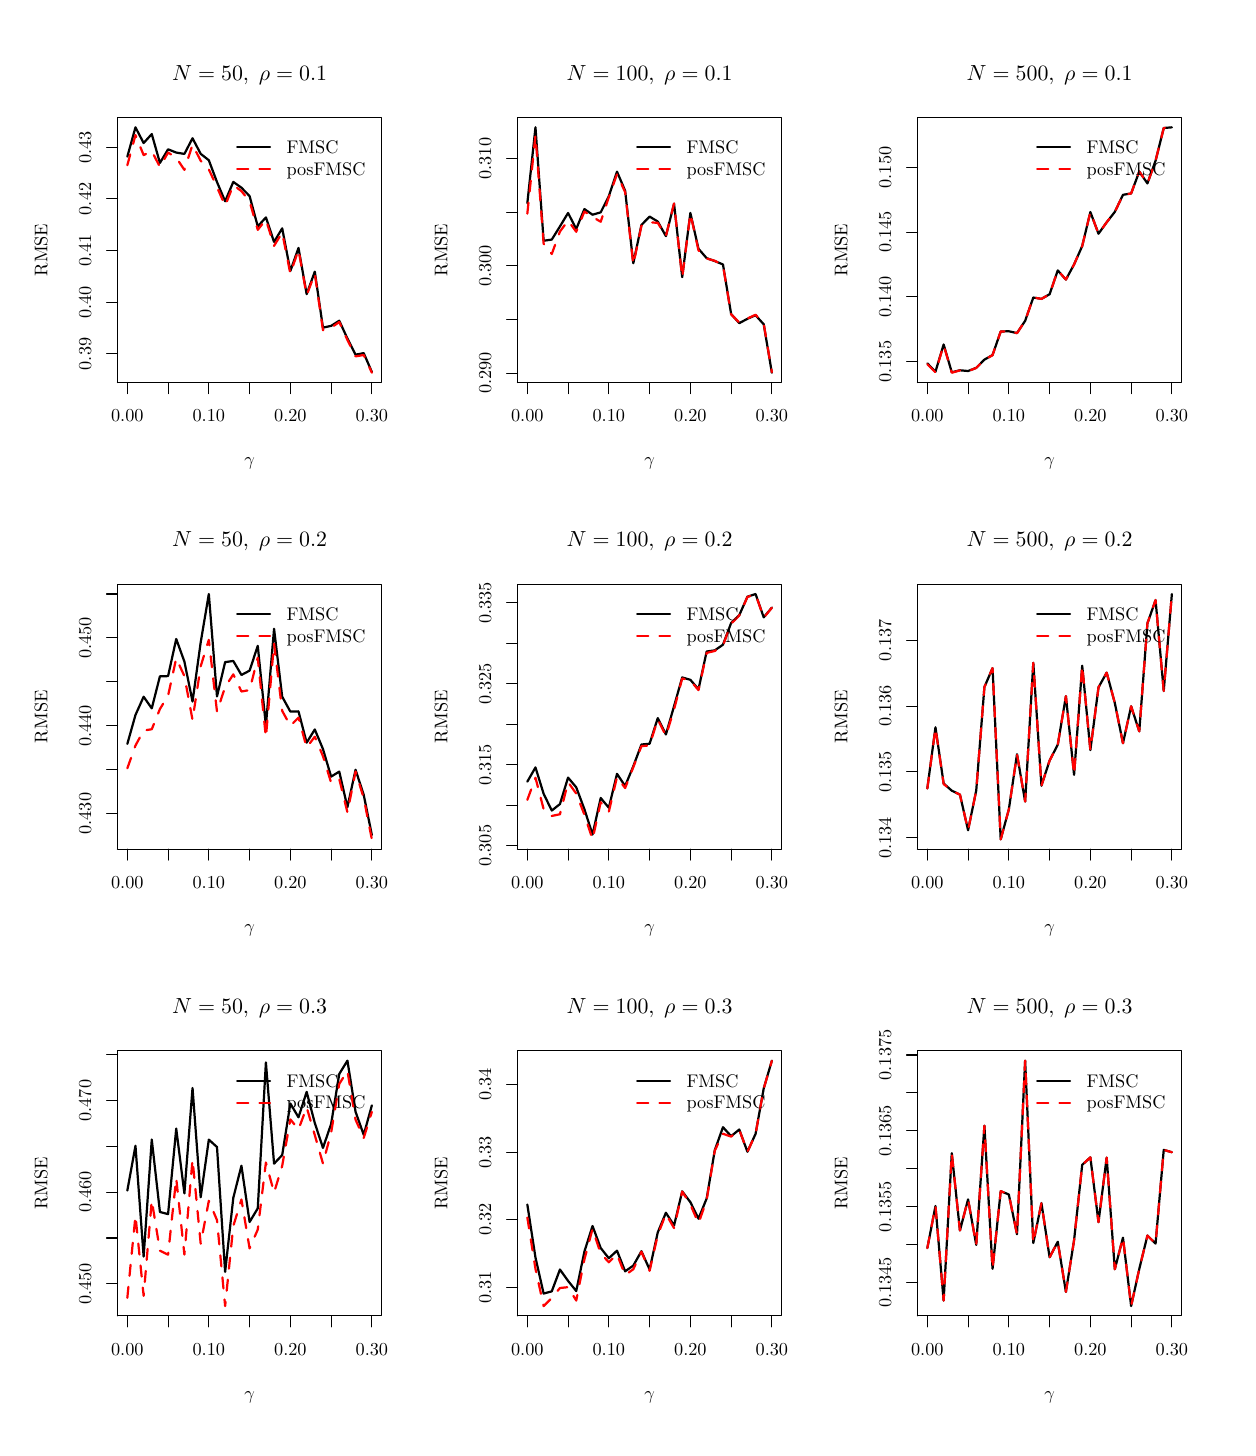
\begin{tikzpicture}[x=1pt,y=1pt]
\definecolor[named]{fillColor}{rgb}{1.00,1.00,1.00}
\path[use as bounding box,fill=fillColor,fill opacity=0.00] (0,0) rectangle (433.62,505.89);
\begin{scope}
\path[clip] ( 32.47,377.65) rectangle (127.91,473.42);
\definecolor[named]{drawColor}{rgb}{0.00,0.00,0.00}

\path[draw=drawColor,line width= 0.8pt,line join=round,line cap=round] ( 36.01,459.27) --
	( 38.95,469.87) --
	( 41.90,464.20) --
	( 44.84,467.44) --
	( 47.79,457.01) --
	( 50.73,461.94) --
	( 53.68,460.75) --
	( 56.63,460.27) --
	( 59.57,465.93) --
	( 62.52,460.29) --
	( 65.46,457.98) --
	( 68.41,450.10) --
	( 71.35,443.15) --
	( 74.30,450.15) --
	( 77.24,448.06) --
	( 80.19,445.03) --
	( 83.14,434.09) --
	( 86.08,437.32) --
	( 89.03,428.46) --
	( 91.97,433.38) --
	( 94.92,417.95) --
	( 97.86,426.29) --
	(100.81,409.59) --
	(103.75,417.72) --
	(106.70,397.48) --
	(109.65,398.14) --
	(112.59,399.99) --
	(115.54,393.54) --
	(118.48,387.71) --
	(121.43,388.29) --
	(124.37,381.47);
\end{scope}
\begin{scope}
\path[clip] (  0.00,  0.00) rectangle (433.62,505.89);
\definecolor[named]{drawColor}{rgb}{0.00,0.00,0.00}

\path[draw=drawColor,line width= 0.4pt,line join=round,line cap=round] ( 36.01,377.65) -- (124.37,377.65);

\path[draw=drawColor,line width= 0.4pt,line join=round,line cap=round] ( 36.01,377.65) -- ( 36.01,373.69);

\path[draw=drawColor,line width= 0.4pt,line join=round,line cap=round] ( 50.73,377.65) -- ( 50.73,373.69);

\path[draw=drawColor,line width= 0.4pt,line join=round,line cap=round] ( 65.46,377.65) -- ( 65.46,373.69);

\path[draw=drawColor,line width= 0.4pt,line join=round,line cap=round] ( 80.19,377.65) -- ( 80.19,373.69);

\path[draw=drawColor,line width= 0.4pt,line join=round,line cap=round] ( 94.92,377.65) -- ( 94.92,373.69);

\path[draw=drawColor,line width= 0.4pt,line join=round,line cap=round] (109.65,377.65) -- (109.65,373.69);

\path[draw=drawColor,line width= 0.4pt,line join=round,line cap=round] (124.37,377.65) -- (124.37,373.69);

\node[text=drawColor,anchor=base,inner sep=0pt, outer sep=0pt, scale=  0.66] at ( 36.01,363.40) {0.00};

\node[text=drawColor,anchor=base,inner sep=0pt, outer sep=0pt, scale=  0.66] at ( 65.46,363.40) {0.10};

\node[text=drawColor,anchor=base,inner sep=0pt, outer sep=0pt, scale=  0.66] at ( 94.92,363.40) {0.20};

\node[text=drawColor,anchor=base,inner sep=0pt, outer sep=0pt, scale=  0.66] at (124.37,363.40) {0.30};

\path[draw=drawColor,line width= 0.4pt,line join=round,line cap=round] ( 32.47,388.00) -- ( 32.47,462.68);

\path[draw=drawColor,line width= 0.4pt,line join=round,line cap=round] ( 32.47,388.00) -- ( 28.51,388.00);

\path[draw=drawColor,line width= 0.4pt,line join=round,line cap=round] ( 32.47,406.67) -- ( 28.51,406.67);

\path[draw=drawColor,line width= 0.4pt,line join=round,line cap=round] ( 32.47,425.34) -- ( 28.51,425.34);

\path[draw=drawColor,line width= 0.4pt,line join=round,line cap=round] ( 32.47,444.01) -- ( 28.51,444.01);

\path[draw=drawColor,line width= 0.4pt,line join=round,line cap=round] ( 32.47,462.68) -- ( 28.51,462.68);

\node[text=drawColor,rotate= 90.00,anchor=base,inner sep=0pt, outer sep=0pt, scale=  0.66] at ( 22.97,388.00) {0.39};

\node[text=drawColor,rotate= 90.00,anchor=base,inner sep=0pt, outer sep=0pt, scale=  0.66] at ( 22.97,406.67) {0.40};

\node[text=drawColor,rotate= 90.00,anchor=base,inner sep=0pt, outer sep=0pt, scale=  0.66] at ( 22.97,425.34) {0.41};

\node[text=drawColor,rotate= 90.00,anchor=base,inner sep=0pt, outer sep=0pt, scale=  0.66] at ( 22.97,444.01) {0.42};

\node[text=drawColor,rotate= 90.00,anchor=base,inner sep=0pt, outer sep=0pt, scale=  0.66] at ( 22.97,462.68) {0.43};

\path[draw=drawColor,line width= 0.4pt,line join=round,line cap=round] ( 32.47,377.65) --
	(127.91,377.65) --
	(127.91,473.42) --
	( 32.47,473.42) --
	( 32.47,377.65);
\end{scope}
\begin{scope}
\path[clip] (  0.00,337.26) rectangle (144.54,505.89);
\definecolor[named]{drawColor}{rgb}{0.00,0.00,0.00}

\node[text=drawColor,anchor=base,inner sep=0pt, outer sep=0pt, scale=  0.79] at ( 80.19,486.92) {\bfseries $N=50, \;\rho=0.1$};

\node[text=drawColor,anchor=base,inner sep=0pt, outer sep=0pt, scale=  0.66] at ( 80.19,347.56) {$\gamma$};

\node[text=drawColor,rotate= 90.00,anchor=base,inner sep=0pt, outer sep=0pt, scale=  0.66] at (  7.13,425.54) {RMSE};
\end{scope}
\begin{scope}
\path[clip] ( 32.47,377.65) rectangle (127.91,473.42);
\definecolor[named]{drawColor}{rgb}{1.00,0.00,0.00}

\path[draw=drawColor,line width= 0.8pt,dash pattern=on 4pt off 4pt ,line join=round,line cap=round] ( 36.01,456.18) --
	( 38.95,467.06) --
	( 41.90,459.85) --
	( 44.84,461.28) --
	( 47.79,455.56) --
	( 50.73,460.76) --
	( 53.68,458.93) --
	( 56.63,454.50) --
	( 59.57,463.59) --
	( 62.52,457.79) --
	( 65.46,454.67) --
	( 68.41,448.28) --
	( 71.35,441.53) --
	( 74.30,448.99) --
	( 77.24,446.83) --
	( 80.19,443.12) --
	( 83.14,432.82) --
	( 86.08,436.55) --
	( 89.03,427.06) --
	( 91.97,431.85) --
	( 94.92,416.97) --
	( 97.86,425.66) --
	(100.81,409.19) --
	(103.75,417.02) --
	(106.70,396.60) --
	(109.65,397.50) --
	(112.59,399.52) --
	(115.54,393.04) --
	(118.48,387.10) --
	(121.43,387.61) --
	(124.37,381.20);
\definecolor[named]{drawColor}{rgb}{0.00,0.00,0.00}

\path[draw=drawColor,line width= 0.8pt,line join=round,line cap=round] ( 75.72,462.63) -- ( 87.60,462.63);
\definecolor[named]{drawColor}{rgb}{1.00,0.00,0.00}

\path[draw=drawColor,line width= 0.8pt,dash pattern=on 4pt off 4pt ,line join=round,line cap=round] ( 75.72,454.71) -- ( 87.60,454.71);
\definecolor[named]{drawColor}{rgb}{0.00,0.00,0.00}

\node[text=drawColor,anchor=base west,inner sep=0pt, outer sep=0pt, scale=  0.66] at ( 93.54,460.35) {FMSC};

\node[text=drawColor,anchor=base west,inner sep=0pt, outer sep=0pt, scale=  0.66] at ( 93.54,452.43) {posFMSC};
\end{scope}
\begin{scope}
\path[clip] (177.01,377.65) rectangle (272.45,473.42);
\definecolor[named]{drawColor}{rgb}{0.00,0.00,0.00}

\path[draw=drawColor,line width= 0.8pt,line join=round,line cap=round] (180.55,442.46) --
	(183.49,469.87) --
	(186.44,428.89) --
	(189.38,429.31) --
	(192.33,434.06) --
	(195.27,438.93) --
	(198.22,433.14) --
	(201.17,440.34) --
	(204.11,438.30) --
	(207.06,439.15) --
	(210.00,445.04) --
	(212.95,453.86) --
	(215.89,446.96) --
	(218.84,420.75) --
	(221.78,434.60) --
	(224.73,437.62) --
	(227.68,435.83) --
	(230.62,430.56) --
	(233.57,442.29) --
	(236.51,415.74) --
	(239.46,438.94) --
	(242.40,425.98) --
	(245.35,422.59) --
	(248.29,421.55) --
	(251.24,420.32) --
	(254.19,402.42) --
	(257.13,399.11) --
	(260.08,400.69) --
	(263.02,401.97) --
	(265.97,398.70) --
	(268.91,381.20);
\end{scope}
\begin{scope}
\path[clip] (  0.00,  0.00) rectangle (433.62,505.89);
\definecolor[named]{drawColor}{rgb}{0.00,0.00,0.00}

\path[draw=drawColor,line width= 0.4pt,line join=round,line cap=round] (180.55,377.65) -- (268.91,377.65);

\path[draw=drawColor,line width= 0.4pt,line join=round,line cap=round] (180.55,377.65) -- (180.55,373.69);

\path[draw=drawColor,line width= 0.4pt,line join=round,line cap=round] (195.27,377.65) -- (195.27,373.69);

\path[draw=drawColor,line width= 0.4pt,line join=round,line cap=round] (210.00,377.65) -- (210.00,373.69);

\path[draw=drawColor,line width= 0.4pt,line join=round,line cap=round] (224.73,377.65) -- (224.73,373.69);

\path[draw=drawColor,line width= 0.4pt,line join=round,line cap=round] (239.46,377.65) -- (239.46,373.69);

\path[draw=drawColor,line width= 0.4pt,line join=round,line cap=round] (254.19,377.65) -- (254.19,373.69);

\path[draw=drawColor,line width= 0.4pt,line join=round,line cap=round] (268.91,377.65) -- (268.91,373.69);

\node[text=drawColor,anchor=base,inner sep=0pt, outer sep=0pt, scale=  0.66] at (180.55,363.40) {0.00};

\node[text=drawColor,anchor=base,inner sep=0pt, outer sep=0pt, scale=  0.66] at (210.00,363.40) {0.10};

\node[text=drawColor,anchor=base,inner sep=0pt, outer sep=0pt, scale=  0.66] at (239.46,363.40) {0.20};

\node[text=drawColor,anchor=base,inner sep=0pt, outer sep=0pt, scale=  0.66] at (268.91,363.40) {0.30};

\path[draw=drawColor,line width= 0.4pt,line join=round,line cap=round] (177.01,381.05) -- (177.01,458.57);

\path[draw=drawColor,line width= 0.4pt,line join=round,line cap=round] (177.01,381.05) -- (173.05,381.05);

\path[draw=drawColor,line width= 0.4pt,line join=round,line cap=round] (177.01,400.43) -- (173.05,400.43);

\path[draw=drawColor,line width= 0.4pt,line join=round,line cap=round] (177.01,419.81) -- (173.05,419.81);

\path[draw=drawColor,line width= 0.4pt,line join=round,line cap=round] (177.01,439.19) -- (173.05,439.19);

\path[draw=drawColor,line width= 0.4pt,line join=round,line cap=round] (177.01,458.57) -- (173.05,458.57);

\node[text=drawColor,rotate= 90.00,anchor=base,inner sep=0pt, outer sep=0pt, scale=  0.66] at (167.51,381.05) {0.290};

\node[text=drawColor,rotate= 90.00,anchor=base,inner sep=0pt, outer sep=0pt, scale=  0.66] at (167.51,419.81) {0.300};

\node[text=drawColor,rotate= 90.00,anchor=base,inner sep=0pt, outer sep=0pt, scale=  0.66] at (167.51,458.57) {0.310};

\path[draw=drawColor,line width= 0.4pt,line join=round,line cap=round] (177.01,377.65) --
	(272.45,377.65) --
	(272.45,473.42) --
	(177.01,473.42) --
	(177.01,377.65);
\end{scope}
\begin{scope}
\path[clip] (144.54,337.26) rectangle (289.08,505.89);
\definecolor[named]{drawColor}{rgb}{0.00,0.00,0.00}

\node[text=drawColor,anchor=base,inner sep=0pt, outer sep=0pt, scale=  0.79] at (224.73,486.92) {\bfseries $N=100, \;\rho=0.1$};

\node[text=drawColor,anchor=base,inner sep=0pt, outer sep=0pt, scale=  0.66] at (224.73,347.56) {$\gamma$};

\node[text=drawColor,rotate= 90.00,anchor=base,inner sep=0pt, outer sep=0pt, scale=  0.66] at (151.67,425.54) {RMSE};
\end{scope}
\begin{scope}
\path[clip] (177.01,377.65) rectangle (272.45,473.42);
\definecolor[named]{drawColor}{rgb}{1.00,0.00,0.00}

\path[draw=drawColor,line width= 0.8pt,dash pattern=on 4pt off 4pt ,line join=round,line cap=round] (180.55,438.68) --
	(183.49,466.99) --
	(186.44,427.83) --
	(189.38,424.10) --
	(192.33,432.21) --
	(195.27,436.17) --
	(198.22,432.14) --
	(201.17,439.45) --
	(204.11,437.50) --
	(207.06,435.75) --
	(210.00,444.63) --
	(212.95,452.94) --
	(215.89,446.45) --
	(218.84,420.26) --
	(221.78,434.26) --
	(224.73,435.53) --
	(227.68,435.37) --
	(230.62,430.60) --
	(233.57,442.36) --
	(236.51,415.60) --
	(239.46,438.74) --
	(242.40,425.39) --
	(245.35,422.49) --
	(248.29,421.64) --
	(251.24,420.05) --
	(254.19,402.29) --
	(257.13,399.33) --
	(260.08,400.78) --
	(263.02,402.15) --
	(265.97,398.93) --
	(268.91,381.38);
\definecolor[named]{drawColor}{rgb}{0.00,0.00,0.00}

\path[draw=drawColor,line width= 0.8pt,line join=round,line cap=round] (220.26,462.63) -- (232.14,462.63);
\definecolor[named]{drawColor}{rgb}{1.00,0.00,0.00}

\path[draw=drawColor,line width= 0.8pt,dash pattern=on 4pt off 4pt ,line join=round,line cap=round] (220.26,454.71) -- (232.14,454.71);
\definecolor[named]{drawColor}{rgb}{0.00,0.00,0.00}

\node[text=drawColor,anchor=base west,inner sep=0pt, outer sep=0pt, scale=  0.66] at (238.08,460.35) {FMSC};

\node[text=drawColor,anchor=base west,inner sep=0pt, outer sep=0pt, scale=  0.66] at (238.08,452.43) {posFMSC};
\end{scope}
\begin{scope}
\path[clip] (321.55,377.65) rectangle (416.99,473.42);
\definecolor[named]{drawColor}{rgb}{0.00,0.00,0.00}

\path[draw=drawColor,line width= 0.8pt,line join=round,line cap=round] (325.09,384.58) --
	(328.03,381.58) --
	(330.98,391.41) --
	(333.92,381.37) --
	(336.87,382.08) --
	(339.81,381.82) --
	(342.76,382.96) --
	(345.71,385.93) --
	(348.65,387.59) --
	(351.60,396.10) --
	(354.54,396.18) --
	(357.49,395.52) --
	(360.43,399.95) --
	(363.38,408.38) --
	(366.32,407.89) --
	(369.27,409.57) --
	(372.22,418.17) --
	(375.16,414.86) --
	(378.11,420.33) --
	(381.05,426.97) --
	(384.00,439.27) --
	(386.94,431.43) --
	(389.89,435.56) --
	(392.83,439.31) --
	(395.78,445.48) --
	(398.73,445.98) --
	(401.67,453.90) --
	(404.62,449.60) --
	(407.56,457.83) --
	(410.51,469.63) --
	(413.45,469.87);
\end{scope}
\begin{scope}
\path[clip] (  0.00,  0.00) rectangle (433.62,505.89);
\definecolor[named]{drawColor}{rgb}{0.00,0.00,0.00}

\path[draw=drawColor,line width= 0.4pt,line join=round,line cap=round] (325.09,377.65) -- (413.45,377.65);

\path[draw=drawColor,line width= 0.4pt,line join=round,line cap=round] (325.09,377.65) -- (325.09,373.69);

\path[draw=drawColor,line width= 0.4pt,line join=round,line cap=round] (339.81,377.65) -- (339.81,373.69);

\path[draw=drawColor,line width= 0.4pt,line join=round,line cap=round] (354.54,377.65) -- (354.54,373.69);

\path[draw=drawColor,line width= 0.4pt,line join=round,line cap=round] (369.27,377.65) -- (369.27,373.69);

\path[draw=drawColor,line width= 0.4pt,line join=round,line cap=round] (384.00,377.65) -- (384.00,373.69);

\path[draw=drawColor,line width= 0.4pt,line join=round,line cap=round] (398.73,377.65) -- (398.73,373.69);

\path[draw=drawColor,line width= 0.4pt,line join=round,line cap=round] (413.45,377.65) -- (413.45,373.69);

\node[text=drawColor,anchor=base,inner sep=0pt, outer sep=0pt, scale=  0.66] at (325.09,363.40) {0.00};

\node[text=drawColor,anchor=base,inner sep=0pt, outer sep=0pt, scale=  0.66] at (354.54,363.40) {0.10};

\node[text=drawColor,anchor=base,inner sep=0pt, outer sep=0pt, scale=  0.66] at (384.00,363.40) {0.20};

\node[text=drawColor,anchor=base,inner sep=0pt, outer sep=0pt, scale=  0.66] at (413.45,363.40) {0.30};

\path[draw=drawColor,line width= 0.4pt,line join=round,line cap=round] (321.55,385.24) -- (321.55,455.38);

\path[draw=drawColor,line width= 0.4pt,line join=round,line cap=round] (321.55,385.24) -- (317.59,385.24);

\path[draw=drawColor,line width= 0.4pt,line join=round,line cap=round] (321.55,408.62) -- (317.59,408.62);

\path[draw=drawColor,line width= 0.4pt,line join=round,line cap=round] (321.55,432.00) -- (317.59,432.00);

\path[draw=drawColor,line width= 0.4pt,line join=round,line cap=round] (321.55,455.38) -- (317.59,455.38);

\node[text=drawColor,rotate= 90.00,anchor=base,inner sep=0pt, outer sep=0pt, scale=  0.66] at (312.05,385.24) {0.135};

\node[text=drawColor,rotate= 90.00,anchor=base,inner sep=0pt, outer sep=0pt, scale=  0.66] at (312.05,408.62) {0.140};

\node[text=drawColor,rotate= 90.00,anchor=base,inner sep=0pt, outer sep=0pt, scale=  0.66] at (312.05,432.00) {0.145};

\node[text=drawColor,rotate= 90.00,anchor=base,inner sep=0pt, outer sep=0pt, scale=  0.66] at (312.05,455.38) {0.150};

\path[draw=drawColor,line width= 0.4pt,line join=round,line cap=round] (321.55,377.65) --
	(416.99,377.65) --
	(416.99,473.42) --
	(321.55,473.42) --
	(321.55,377.65);
\end{scope}
\begin{scope}
\path[clip] (289.08,337.26) rectangle (433.62,505.89);
\definecolor[named]{drawColor}{rgb}{0.00,0.00,0.00}

\node[text=drawColor,anchor=base,inner sep=0pt, outer sep=0pt, scale=  0.79] at (369.27,486.92) {\bfseries $N=500, \;\rho=0.1$};

\node[text=drawColor,anchor=base,inner sep=0pt, outer sep=0pt, scale=  0.66] at (369.27,347.56) {$\gamma$};

\node[text=drawColor,rotate= 90.00,anchor=base,inner sep=0pt, outer sep=0pt, scale=  0.66] at (296.21,425.53) {RMSE};
\end{scope}
\begin{scope}
\path[clip] (321.55,377.65) rectangle (416.99,473.42);
\definecolor[named]{drawColor}{rgb}{1.00,0.00,0.00}

\path[draw=drawColor,line width= 0.8pt,dash pattern=on 4pt off 4pt ,line join=round,line cap=round] (325.09,384.28) --
	(328.03,381.34) --
	(330.98,391.20) --
	(333.92,381.20) --
	(336.87,382.05) --
	(339.81,381.76) --
	(342.76,382.93) --
	(345.71,385.88) --
	(348.65,387.53) --
	(351.60,396.11) --
	(354.54,396.15) --
	(357.49,395.50) --
	(360.43,399.94) --
	(363.38,408.40) --
	(366.32,407.87) --
	(369.27,409.57) --
	(372.22,418.17) --
	(375.16,414.86) --
	(378.11,420.33) --
	(381.05,426.97) --
	(384.00,439.27) --
	(386.94,431.43) --
	(389.89,435.56) --
	(392.83,439.31) --
	(395.78,445.48) --
	(398.73,445.98) --
	(401.67,453.90) --
	(404.62,449.60) --
	(407.56,457.83) --
	(410.51,469.63) --
	(413.45,469.87);
\definecolor[named]{drawColor}{rgb}{0.00,0.00,0.00}

\path[draw=drawColor,line width= 0.8pt,line join=round,line cap=round] (364.80,462.63) -- (376.68,462.63);
\definecolor[named]{drawColor}{rgb}{1.00,0.00,0.00}

\path[draw=drawColor,line width= 0.8pt,dash pattern=on 4pt off 4pt ,line join=round,line cap=round] (364.80,454.71) -- (376.68,454.71);
\definecolor[named]{drawColor}{rgb}{0.00,0.00,0.00}

\node[text=drawColor,anchor=base west,inner sep=0pt, outer sep=0pt, scale=  0.66] at (382.62,460.35) {FMSC};

\node[text=drawColor,anchor=base west,inner sep=0pt, outer sep=0pt, scale=  0.66] at (382.62,452.43) {posFMSC};
\end{scope}
\begin{scope}
\path[clip] ( 32.47,209.02) rectangle (127.91,304.79);
\definecolor[named]{drawColor}{rgb}{0.00,0.00,0.00}

\path[draw=drawColor,line width= 0.8pt,line join=round,line cap=round] ( 36.01,247.07) --
	( 38.95,257.52) --
	( 41.90,264.12) --
	( 44.84,259.92) --
	( 47.79,271.51) --
	( 50.73,271.57) --
	( 53.68,284.99) --
	( 56.63,276.83) --
	( 59.57,262.37) --
	( 62.52,283.78) --
	( 65.46,301.24) --
	( 68.41,264.22) --
	( 71.35,276.63) --
	( 74.30,277.05) --
	( 77.24,271.99) --
	( 80.19,273.55) --
	( 83.14,282.53) --
	( 86.08,253.66) --
	( 89.03,288.68) --
	( 91.97,264.13) --
	( 94.92,258.75) --
	( 97.86,258.84) --
	(100.81,247.53) --
	(103.75,252.30) --
	(106.70,245.23) --
	(109.65,235.25) --
	(112.59,237.07) --
	(115.54,224.21) --
	(118.48,237.74) --
	(121.43,228.67) --
	(124.37,214.16);
\end{scope}
\begin{scope}
\path[clip] (  0.00,  0.00) rectangle (433.62,505.89);
\definecolor[named]{drawColor}{rgb}{0.00,0.00,0.00}

\path[draw=drawColor,line width= 0.4pt,line join=round,line cap=round] ( 36.01,209.02) -- (124.37,209.02);

\path[draw=drawColor,line width= 0.4pt,line join=round,line cap=round] ( 36.01,209.02) -- ( 36.01,205.06);

\path[draw=drawColor,line width= 0.4pt,line join=round,line cap=round] ( 50.73,209.02) -- ( 50.73,205.06);

\path[draw=drawColor,line width= 0.4pt,line join=round,line cap=round] ( 65.46,209.02) -- ( 65.46,205.06);

\path[draw=drawColor,line width= 0.4pt,line join=round,line cap=round] ( 80.19,209.02) -- ( 80.19,205.06);

\path[draw=drawColor,line width= 0.4pt,line join=round,line cap=round] ( 94.92,209.02) -- ( 94.92,205.06);

\path[draw=drawColor,line width= 0.4pt,line join=round,line cap=round] (109.65,209.02) -- (109.65,205.06);

\path[draw=drawColor,line width= 0.4pt,line join=round,line cap=round] (124.37,209.02) -- (124.37,205.06);

\node[text=drawColor,anchor=base,inner sep=0pt, outer sep=0pt, scale=  0.66] at ( 36.01,194.77) {0.00};

\node[text=drawColor,anchor=base,inner sep=0pt, outer sep=0pt, scale=  0.66] at ( 65.46,194.77) {0.10};

\node[text=drawColor,anchor=base,inner sep=0pt, outer sep=0pt, scale=  0.66] at ( 94.92,194.77) {0.20};

\node[text=drawColor,anchor=base,inner sep=0pt, outer sep=0pt, scale=  0.66] at (124.37,194.77) {0.30};

\path[draw=drawColor,line width= 0.4pt,line join=round,line cap=round] ( 32.47,221.88) -- ( 32.47,301.26);

\path[draw=drawColor,line width= 0.4pt,line join=round,line cap=round] ( 32.47,221.88) -- ( 28.51,221.88);

\path[draw=drawColor,line width= 0.4pt,line join=round,line cap=round] ( 32.47,237.76) -- ( 28.51,237.76);

\path[draw=drawColor,line width= 0.4pt,line join=round,line cap=round] ( 32.47,253.63) -- ( 28.51,253.63);

\path[draw=drawColor,line width= 0.4pt,line join=round,line cap=round] ( 32.47,269.51) -- ( 28.51,269.51);

\path[draw=drawColor,line width= 0.4pt,line join=round,line cap=round] ( 32.47,285.38) -- ( 28.51,285.38);

\path[draw=drawColor,line width= 0.4pt,line join=round,line cap=round] ( 32.47,301.26) -- ( 28.51,301.26);

\node[text=drawColor,rotate= 90.00,anchor=base,inner sep=0pt, outer sep=0pt, scale=  0.66] at ( 22.97,221.88) {0.430};

\node[text=drawColor,rotate= 90.00,anchor=base,inner sep=0pt, outer sep=0pt, scale=  0.66] at ( 22.97,253.63) {0.440};

\node[text=drawColor,rotate= 90.00,anchor=base,inner sep=0pt, outer sep=0pt, scale=  0.66] at ( 22.97,285.38) {0.450};

\path[draw=drawColor,line width= 0.4pt,line join=round,line cap=round] ( 32.47,209.02) --
	(127.91,209.02) --
	(127.91,304.79) --
	( 32.47,304.79) --
	( 32.47,209.02);
\end{scope}
\begin{scope}
\path[clip] (  0.00,168.63) rectangle (144.54,337.26);
\definecolor[named]{drawColor}{rgb}{0.00,0.00,0.00}

\node[text=drawColor,anchor=base,inner sep=0pt, outer sep=0pt, scale=  0.79] at ( 80.19,318.29) {\bfseries $N=50, \;\rho=0.2$};

\node[text=drawColor,anchor=base,inner sep=0pt, outer sep=0pt, scale=  0.66] at ( 80.19,178.93) {$\gamma$};

\node[text=drawColor,rotate= 90.00,anchor=base,inner sep=0pt, outer sep=0pt, scale=  0.66] at (  7.13,256.90) {RMSE};
\end{scope}
\begin{scope}
\path[clip] ( 32.47,209.02) rectangle (127.91,304.79);
\definecolor[named]{drawColor}{rgb}{1.00,0.00,0.00}

\path[draw=drawColor,line width= 0.8pt,dash pattern=on 4pt off 4pt ,line join=round,line cap=round] ( 36.01,238.26) --
	( 38.95,246.48) --
	( 41.90,251.92) --
	( 44.84,252.37) --
	( 47.79,259.69) --
	( 50.73,264.49) --
	( 53.68,278.00) --
	( 56.63,271.58) --
	( 59.57,255.75) --
	( 62.52,275.14) --
	( 65.46,284.69) --
	( 68.41,258.73) --
	( 71.35,267.65) --
	( 74.30,272.21) --
	( 77.24,266.02) --
	( 80.19,266.52) --
	( 83.14,278.22) --
	( 86.08,249.41) --
	( 89.03,283.37) --
	( 91.97,259.02) --
	( 94.92,253.60) --
	( 97.86,256.58) --
	(100.81,245.77) --
	(103.75,249.69) --
	(106.70,242.66) --
	(109.65,233.06) --
	(112.59,234.38) --
	(115.54,222.36) --
	(118.48,237.10) --
	(121.43,227.51) --
	(124.37,212.57);
\definecolor[named]{drawColor}{rgb}{0.00,0.00,0.00}

\path[draw=drawColor,line width= 0.8pt,line join=round,line cap=round] ( 75.72,294.00) -- ( 87.60,294.00);
\definecolor[named]{drawColor}{rgb}{1.00,0.00,0.00}

\path[draw=drawColor,line width= 0.8pt,dash pattern=on 4pt off 4pt ,line join=round,line cap=round] ( 75.72,286.08) -- ( 87.60,286.08);
\definecolor[named]{drawColor}{rgb}{0.00,0.00,0.00}

\node[text=drawColor,anchor=base west,inner sep=0pt, outer sep=0pt, scale=  0.66] at ( 93.54,291.72) {FMSC};

\node[text=drawColor,anchor=base west,inner sep=0pt, outer sep=0pt, scale=  0.66] at ( 93.54,283.80) {posFMSC};
\end{scope}
\begin{scope}
\path[clip] (177.01,209.02) rectangle (272.45,304.79);
\definecolor[named]{drawColor}{rgb}{0.00,0.00,0.00}

\path[draw=drawColor,line width= 0.8pt,line join=round,line cap=round] (180.55,233.44) --
	(183.49,238.58) --
	(186.44,229.06) --
	(189.38,222.99) --
	(192.33,225.33) --
	(195.27,234.91) --
	(198.22,231.38) --
	(201.17,223.50) --
	(204.11,214.31) --
	(207.06,227.54) --
	(210.00,224.01) --
	(212.95,236.27) --
	(215.89,231.87) --
	(218.84,239.00) --
	(221.78,246.85) --
	(224.73,247.14) --
	(227.68,256.39) --
	(230.62,250.48) --
	(233.57,260.71) --
	(236.51,271.09) --
	(239.46,270.24) --
	(242.40,266.82) --
	(245.35,280.47) --
	(248.29,280.88) --
	(251.24,282.91) --
	(254.19,290.77) --
	(257.13,293.60) --
	(260.08,300.26) --
	(263.02,301.24) --
	(265.97,292.81) --
	(268.91,296.35);
\end{scope}
\begin{scope}
\path[clip] (  0.00,  0.00) rectangle (433.62,505.89);
\definecolor[named]{drawColor}{rgb}{0.00,0.00,0.00}

\path[draw=drawColor,line width= 0.4pt,line join=round,line cap=round] (180.55,209.02) -- (268.91,209.02);

\path[draw=drawColor,line width= 0.4pt,line join=round,line cap=round] (180.55,209.02) -- (180.55,205.06);

\path[draw=drawColor,line width= 0.4pt,line join=round,line cap=round] (195.27,209.02) -- (195.27,205.06);

\path[draw=drawColor,line width= 0.4pt,line join=round,line cap=round] (210.00,209.02) -- (210.00,205.06);

\path[draw=drawColor,line width= 0.4pt,line join=round,line cap=round] (224.73,209.02) -- (224.73,205.06);

\path[draw=drawColor,line width= 0.4pt,line join=round,line cap=round] (239.46,209.02) -- (239.46,205.06);

\path[draw=drawColor,line width= 0.4pt,line join=round,line cap=round] (254.19,209.02) -- (254.19,205.06);

\path[draw=drawColor,line width= 0.4pt,line join=round,line cap=round] (268.91,209.02) -- (268.91,205.06);

\node[text=drawColor,anchor=base,inner sep=0pt, outer sep=0pt, scale=  0.66] at (180.55,194.77) {0.00};

\node[text=drawColor,anchor=base,inner sep=0pt, outer sep=0pt, scale=  0.66] at (210.00,194.77) {0.10};

\node[text=drawColor,anchor=base,inner sep=0pt, outer sep=0pt, scale=  0.66] at (239.46,194.77) {0.20};

\node[text=drawColor,anchor=base,inner sep=0pt, outer sep=0pt, scale=  0.66] at (268.91,194.77) {0.30};

\path[draw=drawColor,line width= 0.4pt,line join=round,line cap=round] (177.01,210.31) -- (177.01,298.05);

\path[draw=drawColor,line width= 0.4pt,line join=round,line cap=round] (177.01,210.31) -- (173.05,210.31);

\path[draw=drawColor,line width= 0.4pt,line join=round,line cap=round] (177.01,224.93) -- (173.05,224.93);

\path[draw=drawColor,line width= 0.4pt,line join=round,line cap=round] (177.01,239.56) -- (173.05,239.56);

\path[draw=drawColor,line width= 0.4pt,line join=round,line cap=round] (177.01,254.18) -- (173.05,254.18);

\path[draw=drawColor,line width= 0.4pt,line join=round,line cap=round] (177.01,268.80) -- (173.05,268.80);

\path[draw=drawColor,line width= 0.4pt,line join=round,line cap=round] (177.01,283.43) -- (173.05,283.43);

\path[draw=drawColor,line width= 0.4pt,line join=round,line cap=round] (177.01,298.05) -- (173.05,298.05);

\node[text=drawColor,rotate= 90.00,anchor=base,inner sep=0pt, outer sep=0pt, scale=  0.66] at (167.51,210.31) {0.305};

\node[text=drawColor,rotate= 90.00,anchor=base,inner sep=0pt, outer sep=0pt, scale=  0.66] at (167.51,239.56) {0.315};

\node[text=drawColor,rotate= 90.00,anchor=base,inner sep=0pt, outer sep=0pt, scale=  0.66] at (167.51,268.80) {0.325};

\node[text=drawColor,rotate= 90.00,anchor=base,inner sep=0pt, outer sep=0pt, scale=  0.66] at (167.51,298.05) {0.335};

\path[draw=drawColor,line width= 0.4pt,line join=round,line cap=round] (177.01,209.02) --
	(272.45,209.02) --
	(272.45,304.79) --
	(177.01,304.79) --
	(177.01,209.02);
\end{scope}
\begin{scope}
\path[clip] (144.54,168.63) rectangle (289.08,337.26);
\definecolor[named]{drawColor}{rgb}{0.00,0.00,0.00}

\node[text=drawColor,anchor=base,inner sep=0pt, outer sep=0pt, scale=  0.79] at (224.73,318.29) {\bfseries $N=100, \;\rho=0.2$};

\node[text=drawColor,anchor=base,inner sep=0pt, outer sep=0pt, scale=  0.66] at (224.73,178.93) {$\gamma$};

\node[text=drawColor,rotate= 90.00,anchor=base,inner sep=0pt, outer sep=0pt, scale=  0.66] at (151.67,256.91) {RMSE};
\end{scope}
\begin{scope}
\path[clip] (177.01,209.02) rectangle (272.45,304.79);
\definecolor[named]{drawColor}{rgb}{1.00,0.00,0.00}

\path[draw=drawColor,line width= 0.8pt,dash pattern=on 4pt off 4pt ,line join=round,line cap=round] (180.55,226.86) --
	(183.49,234.85) --
	(186.44,223.50) --
	(189.38,221.05) --
	(192.33,221.65) --
	(195.27,233.24) --
	(198.22,229.13) --
	(201.17,221.53) --
	(204.11,212.57) --
	(207.06,226.00) --
	(210.00,222.58) --
	(212.95,235.08) --
	(215.89,231.12) --
	(218.84,238.67) --
	(221.78,246.26) --
	(224.73,246.53) --
	(227.68,255.98) --
	(230.62,249.98) --
	(233.57,259.55) --
	(236.51,270.72) --
	(239.46,270.00) --
	(242.40,266.50) --
	(245.35,279.96) --
	(248.29,280.66) --
	(251.24,282.62) --
	(254.19,290.56) --
	(257.13,293.48) --
	(260.08,300.17) --
	(263.02,301.13) --
	(265.97,292.66) --
	(268.91,296.27);
\definecolor[named]{drawColor}{rgb}{0.00,0.00,0.00}

\path[draw=drawColor,line width= 0.8pt,line join=round,line cap=round] (220.26,294.00) -- (232.14,294.00);
\definecolor[named]{drawColor}{rgb}{1.00,0.00,0.00}

\path[draw=drawColor,line width= 0.8pt,dash pattern=on 4pt off 4pt ,line join=round,line cap=round] (220.26,286.08) -- (232.14,286.08);
\definecolor[named]{drawColor}{rgb}{0.00,0.00,0.00}

\node[text=drawColor,anchor=base west,inner sep=0pt, outer sep=0pt, scale=  0.66] at (238.08,291.72) {FMSC};

\node[text=drawColor,anchor=base west,inner sep=0pt, outer sep=0pt, scale=  0.66] at (238.08,283.80) {posFMSC};
\end{scope}
\begin{scope}
\path[clip] (321.55,209.02) rectangle (416.99,304.79);
\definecolor[named]{drawColor}{rgb}{0.00,0.00,0.00}

\path[draw=drawColor,line width= 0.8pt,line join=round,line cap=round] (325.09,230.99) --
	(328.03,253.08) --
	(330.98,232.77) --
	(333.92,230.18) --
	(336.87,228.76) --
	(339.81,215.88) --
	(342.76,230.26) --
	(345.71,267.60) --
	(348.65,274.47) --
	(351.60,212.57) --
	(354.54,223.42) --
	(357.49,243.36) --
	(360.43,226.26) --
	(363.38,276.37) --
	(366.32,231.96) --
	(369.27,241.07) --
	(372.22,246.79) --
	(375.16,264.33) --
	(378.11,235.91) --
	(381.05,275.34) --
	(384.00,244.83) --
	(386.94,267.52) --
	(389.89,272.83) --
	(392.83,261.88) --
	(395.78,247.32) --
	(398.73,260.66) --
	(401.67,251.61) --
	(404.62,290.64) --
	(407.56,299.06) --
	(410.51,266.22) --
	(413.45,301.24);
\end{scope}
\begin{scope}
\path[clip] (  0.00,  0.00) rectangle (433.62,505.89);
\definecolor[named]{drawColor}{rgb}{0.00,0.00,0.00}

\path[draw=drawColor,line width= 0.4pt,line join=round,line cap=round] (325.09,209.02) -- (413.45,209.02);

\path[draw=drawColor,line width= 0.4pt,line join=round,line cap=round] (325.09,209.02) -- (325.09,205.06);

\path[draw=drawColor,line width= 0.4pt,line join=round,line cap=round] (339.81,209.02) -- (339.81,205.06);

\path[draw=drawColor,line width= 0.4pt,line join=round,line cap=round] (354.54,209.02) -- (354.54,205.06);

\path[draw=drawColor,line width= 0.4pt,line join=round,line cap=round] (369.27,209.02) -- (369.27,205.06);

\path[draw=drawColor,line width= 0.4pt,line join=round,line cap=round] (384.00,209.02) -- (384.00,205.06);

\path[draw=drawColor,line width= 0.4pt,line join=round,line cap=round] (398.73,209.02) -- (398.73,205.06);

\path[draw=drawColor,line width= 0.4pt,line join=round,line cap=round] (413.45,209.02) -- (413.45,205.06);

\node[text=drawColor,anchor=base,inner sep=0pt, outer sep=0pt, scale=  0.66] at (325.09,194.77) {0.00};

\node[text=drawColor,anchor=base,inner sep=0pt, outer sep=0pt, scale=  0.66] at (354.54,194.77) {0.10};

\node[text=drawColor,anchor=base,inner sep=0pt, outer sep=0pt, scale=  0.66] at (384.00,194.77) {0.20};

\node[text=drawColor,anchor=base,inner sep=0pt, outer sep=0pt, scale=  0.66] at (413.45,194.77) {0.30};

\path[draw=drawColor,line width= 0.4pt,line join=round,line cap=round] (321.55,213.15) -- (321.55,284.54);

\path[draw=drawColor,line width= 0.4pt,line join=round,line cap=round] (321.55,213.15) -- (317.59,213.15);

\path[draw=drawColor,line width= 0.4pt,line join=round,line cap=round] (321.55,236.95) -- (317.59,236.95);

\path[draw=drawColor,line width= 0.4pt,line join=round,line cap=round] (321.55,260.74) -- (317.59,260.74);

\path[draw=drawColor,line width= 0.4pt,line join=round,line cap=round] (321.55,284.54) -- (317.59,284.54);

\node[text=drawColor,rotate= 90.00,anchor=base,inner sep=0pt, outer sep=0pt, scale=  0.66] at (312.05,213.15) {0.134};

\node[text=drawColor,rotate= 90.00,anchor=base,inner sep=0pt, outer sep=0pt, scale=  0.66] at (312.05,236.95) {0.135};

\node[text=drawColor,rotate= 90.00,anchor=base,inner sep=0pt, outer sep=0pt, scale=  0.66] at (312.05,260.74) {0.136};

\node[text=drawColor,rotate= 90.00,anchor=base,inner sep=0pt, outer sep=0pt, scale=  0.66] at (312.05,284.54) {0.137};

\path[draw=drawColor,line width= 0.4pt,line join=round,line cap=round] (321.55,209.02) --
	(416.99,209.02) --
	(416.99,304.79) --
	(321.55,304.79) --
	(321.55,209.02);
\end{scope}
\begin{scope}
\path[clip] (289.08,168.63) rectangle (433.62,337.26);
\definecolor[named]{drawColor}{rgb}{0.00,0.00,0.00}

\node[text=drawColor,anchor=base,inner sep=0pt, outer sep=0pt, scale=  0.79] at (369.27,318.29) {\bfseries $N=500, \;\rho=0.2$};

\node[text=drawColor,anchor=base,inner sep=0pt, outer sep=0pt, scale=  0.66] at (369.27,178.93) {$\gamma$};

\node[text=drawColor,rotate= 90.00,anchor=base,inner sep=0pt, outer sep=0pt, scale=  0.66] at (296.21,256.90) {RMSE};
\end{scope}
\begin{scope}
\path[clip] (321.55,209.02) rectangle (416.99,304.79);
\definecolor[named]{drawColor}{rgb}{1.00,0.00,0.00}

\path[draw=drawColor,line width= 0.8pt,dash pattern=on 4pt off 4pt ,line join=round,line cap=round] (325.09,230.99) --
	(328.03,252.82) --
	(330.98,232.57) --
	(333.92,230.18) --
	(336.87,228.75) --
	(339.81,215.88) --
	(342.76,230.21) --
	(345.71,267.60) --
	(348.65,274.47) --
	(351.60,212.57) --
	(354.54,223.42) --
	(357.49,243.36) --
	(360.43,226.26) --
	(363.38,276.37) --
	(366.32,231.96) --
	(369.27,241.07) --
	(372.22,246.78) --
	(375.16,264.33) --
	(378.11,235.91) --
	(381.05,275.34) --
	(384.00,244.83) --
	(386.94,267.52) --
	(389.89,272.83) --
	(392.83,261.88) --
	(395.78,247.32) --
	(398.73,260.66) --
	(401.67,251.61) --
	(404.62,290.64) --
	(407.56,299.06) --
	(410.51,266.22) --
	(413.45,301.24);
\definecolor[named]{drawColor}{rgb}{0.00,0.00,0.00}

\path[draw=drawColor,line width= 0.8pt,line join=round,line cap=round] (364.80,294.00) -- (376.68,294.00);
\definecolor[named]{drawColor}{rgb}{1.00,0.00,0.00}

\path[draw=drawColor,line width= 0.8pt,dash pattern=on 4pt off 4pt ,line join=round,line cap=round] (364.80,286.08) -- (376.68,286.08);
\definecolor[named]{drawColor}{rgb}{0.00,0.00,0.00}

\node[text=drawColor,anchor=base west,inner sep=0pt, outer sep=0pt, scale=  0.66] at (382.62,291.72) {FMSC};

\node[text=drawColor,anchor=base west,inner sep=0pt, outer sep=0pt, scale=  0.66] at (382.62,283.80) {posFMSC};
\end{scope}
\begin{scope}
\path[clip] ( 32.47, 40.39) rectangle (127.91,136.16);
\definecolor[named]{drawColor}{rgb}{0.00,0.00,0.00}

\path[draw=drawColor,line width= 0.8pt,line join=round,line cap=round] ( 36.01, 85.67) --
	( 38.95,101.87) --
	( 41.90, 61.83) --
	( 44.84,104.10) --
	( 47.79, 77.94) --
	( 50.73, 77.17) --
	( 53.68,108.07) --
	( 56.63, 84.64) --
	( 59.57,122.75) --
	( 62.52, 83.25) --
	( 65.46,104.08) --
	( 68.41,101.41) --
	( 71.35, 56.27) --
	( 74.30, 83.04) --
	( 77.24, 94.67) --
	( 80.19, 74.33) --
	( 83.14, 79.25) --
	( 86.08,131.97) --
	( 89.03, 95.39) --
	( 91.97, 98.51) --
	( 94.92,117.13) --
	( 97.86,112.15) --
	(100.81,121.34) --
	(103.75,110.09) --
	(106.70,101.09) --
	(109.65,109.74) --
	(112.59,127.82) --
	(115.54,132.61) --
	(118.48,114.15) --
	(121.43,105.81) --
	(124.37,116.46);
\end{scope}
\begin{scope}
\path[clip] (  0.00,  0.00) rectangle (433.62,505.89);
\definecolor[named]{drawColor}{rgb}{0.00,0.00,0.00}

\path[draw=drawColor,line width= 0.4pt,line join=round,line cap=round] ( 36.01, 40.39) -- (124.37, 40.39);

\path[draw=drawColor,line width= 0.4pt,line join=round,line cap=round] ( 36.01, 40.39) -- ( 36.01, 36.43);

\path[draw=drawColor,line width= 0.4pt,line join=round,line cap=round] ( 50.73, 40.39) -- ( 50.73, 36.43);

\path[draw=drawColor,line width= 0.4pt,line join=round,line cap=round] ( 65.46, 40.39) -- ( 65.46, 36.43);

\path[draw=drawColor,line width= 0.4pt,line join=round,line cap=round] ( 80.19, 40.39) -- ( 80.19, 36.43);

\path[draw=drawColor,line width= 0.4pt,line join=round,line cap=round] ( 94.92, 40.39) -- ( 94.92, 36.43);

\path[draw=drawColor,line width= 0.4pt,line join=round,line cap=round] (109.65, 40.39) -- (109.65, 36.43);

\path[draw=drawColor,line width= 0.4pt,line join=round,line cap=round] (124.37, 40.39) -- (124.37, 36.43);

\node[text=drawColor,anchor=base,inner sep=0pt, outer sep=0pt, scale=  0.66] at ( 36.01, 26.14) {0.00};

\node[text=drawColor,anchor=base,inner sep=0pt, outer sep=0pt, scale=  0.66] at ( 65.46, 26.14) {0.10};

\node[text=drawColor,anchor=base,inner sep=0pt, outer sep=0pt, scale=  0.66] at ( 94.92, 26.14) {0.20};

\node[text=drawColor,anchor=base,inner sep=0pt, outer sep=0pt, scale=  0.66] at (124.37, 26.14) {0.30};

\path[draw=drawColor,line width= 0.4pt,line join=round,line cap=round] ( 32.47, 51.96) -- ( 32.47,134.78);

\path[draw=drawColor,line width= 0.4pt,line join=round,line cap=round] ( 32.47, 51.96) -- ( 28.51, 51.96);

\path[draw=drawColor,line width= 0.4pt,line join=round,line cap=round] ( 32.47, 68.53) -- ( 28.51, 68.53);

\path[draw=drawColor,line width= 0.4pt,line join=round,line cap=round] ( 32.47, 85.09) -- ( 28.51, 85.09);

\path[draw=drawColor,line width= 0.4pt,line join=round,line cap=round] ( 32.47,101.65) -- ( 28.51,101.65);

\path[draw=drawColor,line width= 0.4pt,line join=round,line cap=round] ( 32.47,118.21) -- ( 28.51,118.21);

\path[draw=drawColor,line width= 0.4pt,line join=round,line cap=round] ( 32.47,134.78) -- ( 28.51,134.78);

\node[text=drawColor,rotate= 90.00,anchor=base,inner sep=0pt, outer sep=0pt, scale=  0.66] at ( 22.97, 51.96) {0.450};

\node[text=drawColor,rotate= 90.00,anchor=base,inner sep=0pt, outer sep=0pt, scale=  0.66] at ( 22.97, 85.09) {0.460};

\node[text=drawColor,rotate= 90.00,anchor=base,inner sep=0pt, outer sep=0pt, scale=  0.66] at ( 22.97,118.21) {0.470};

\path[draw=drawColor,line width= 0.4pt,line join=round,line cap=round] ( 32.47, 40.39) --
	(127.91, 40.39) --
	(127.91,136.16) --
	( 32.47,136.16) --
	( 32.47, 40.39);
\end{scope}
\begin{scope}
\path[clip] (  0.00,  0.00) rectangle (144.54,168.63);
\definecolor[named]{drawColor}{rgb}{0.00,0.00,0.00}

\node[text=drawColor,anchor=base,inner sep=0pt, outer sep=0pt, scale=  0.79] at ( 80.19,149.66) {\bfseries $N=50, \;\rho=0.3$};

\node[text=drawColor,anchor=base,inner sep=0pt, outer sep=0pt, scale=  0.66] at ( 80.19, 10.30) {$\gamma$};

\node[text=drawColor,rotate= 90.00,anchor=base,inner sep=0pt, outer sep=0pt, scale=  0.66] at (  7.13, 88.27) {RMSE};
\end{scope}
\begin{scope}
\path[clip] ( 32.47, 40.39) rectangle (127.91,136.16);
\definecolor[named]{drawColor}{rgb}{1.00,0.00,0.00}

\path[draw=drawColor,line width= 0.8pt,dash pattern=on 4pt off 4pt ,line join=round,line cap=round] ( 36.01, 46.91) --
	( 38.95, 76.62) --
	( 41.90, 47.65) --
	( 44.84, 82.13) --
	( 47.79, 63.96) --
	( 50.73, 62.50) --
	( 53.68, 90.13) --
	( 56.63, 62.55) --
	( 59.57, 96.92) --
	( 62.52, 66.48) --
	( 65.46, 81.97) --
	( 68.41, 75.01) --
	( 71.35, 43.94) --
	( 74.30, 72.85) --
	( 77.24, 82.45) --
	( 80.19, 64.79) --
	( 83.14, 71.58) --
	( 86.08, 95.81) --
	( 89.03, 84.93) --
	( 91.97, 94.61) --
	( 94.92,111.41) --
	( 97.86,107.76) --
	(100.81,115.78) --
	(103.75,105.72) --
	(106.70, 95.47) --
	(109.65,106.62) --
	(112.59,124.21) --
	(115.54,128.89) --
	(118.48,111.28) --
	(121.43,104.71) --
	(124.37,114.12);
\definecolor[named]{drawColor}{rgb}{0.00,0.00,0.00}

\path[draw=drawColor,line width= 0.8pt,line join=round,line cap=round] ( 75.72,125.37) -- ( 87.60,125.37);
\definecolor[named]{drawColor}{rgb}{1.00,0.00,0.00}

\path[draw=drawColor,line width= 0.8pt,dash pattern=on 4pt off 4pt ,line join=round,line cap=round] ( 75.72,117.45) -- ( 87.60,117.45);
\definecolor[named]{drawColor}{rgb}{0.00,0.00,0.00}

\node[text=drawColor,anchor=base west,inner sep=0pt, outer sep=0pt, scale=  0.66] at ( 93.54,123.09) {FMSC};

\node[text=drawColor,anchor=base west,inner sep=0pt, outer sep=0pt, scale=  0.66] at ( 93.54,115.17) {posFMSC};
\end{scope}
\begin{scope}
\path[clip] (177.01, 40.39) rectangle (272.45,136.16);
\definecolor[named]{drawColor}{rgb}{0.00,0.00,0.00}

\path[draw=drawColor,line width= 0.8pt,line join=round,line cap=round] (180.55, 80.62) --
	(183.49, 61.48) --
	(186.44, 48.46) --
	(189.38, 49.26) --
	(192.33, 57.15) --
	(195.27, 53.04) --
	(198.22, 49.37) --
	(201.17, 63.63) --
	(204.11, 72.88) --
	(207.06, 64.92) --
	(210.00, 61.22) --
	(212.95, 63.96) --
	(215.89, 56.50) --
	(218.84, 58.56) --
	(221.78, 63.77) --
	(224.73, 57.16) --
	(227.68, 70.56) --
	(230.62, 77.66) --
	(233.57, 73.06) --
	(236.51, 85.40) --
	(239.46, 81.49) --
	(242.40, 75.52) --
	(245.35, 82.82) --
	(248.29,100.28) --
	(251.24,108.58) --
	(254.19,105.34) --
	(257.13,107.73) --
	(260.08, 99.71) --
	(263.02,106.16) --
	(265.97,122.59) --
	(268.91,132.61);
\end{scope}
\begin{scope}
\path[clip] (  0.00,  0.00) rectangle (433.62,505.89);
\definecolor[named]{drawColor}{rgb}{0.00,0.00,0.00}

\path[draw=drawColor,line width= 0.4pt,line join=round,line cap=round] (180.55, 40.39) -- (268.91, 40.39);

\path[draw=drawColor,line width= 0.4pt,line join=round,line cap=round] (180.55, 40.39) -- (180.55, 36.43);

\path[draw=drawColor,line width= 0.4pt,line join=round,line cap=round] (195.27, 40.39) -- (195.27, 36.43);

\path[draw=drawColor,line width= 0.4pt,line join=round,line cap=round] (210.00, 40.39) -- (210.00, 36.43);

\path[draw=drawColor,line width= 0.4pt,line join=round,line cap=round] (224.73, 40.39) -- (224.73, 36.43);

\path[draw=drawColor,line width= 0.4pt,line join=round,line cap=round] (239.46, 40.39) -- (239.46, 36.43);

\path[draw=drawColor,line width= 0.4pt,line join=round,line cap=round] (254.19, 40.39) -- (254.19, 36.43);

\path[draw=drawColor,line width= 0.4pt,line join=round,line cap=round] (268.91, 40.39) -- (268.91, 36.43);

\node[text=drawColor,anchor=base,inner sep=0pt, outer sep=0pt, scale=  0.66] at (180.55, 26.14) {0.00};

\node[text=drawColor,anchor=base,inner sep=0pt, outer sep=0pt, scale=  0.66] at (210.00, 26.14) {0.10};

\node[text=drawColor,anchor=base,inner sep=0pt, outer sep=0pt, scale=  0.66] at (239.46, 26.14) {0.20};

\node[text=drawColor,anchor=base,inner sep=0pt, outer sep=0pt, scale=  0.66] at (268.91, 26.14) {0.30};

\path[draw=drawColor,line width= 0.4pt,line join=round,line cap=round] (177.01, 50.72) -- (177.01,123.94);

\path[draw=drawColor,line width= 0.4pt,line join=round,line cap=round] (177.01, 50.72) -- (173.05, 50.72);

\path[draw=drawColor,line width= 0.4pt,line join=round,line cap=round] (177.01, 75.13) -- (173.05, 75.13);

\path[draw=drawColor,line width= 0.4pt,line join=round,line cap=round] (177.01, 99.53) -- (173.05, 99.53);

\path[draw=drawColor,line width= 0.4pt,line join=round,line cap=round] (177.01,123.94) -- (173.05,123.94);

\node[text=drawColor,rotate= 90.00,anchor=base,inner sep=0pt, outer sep=0pt, scale=  0.66] at (167.51, 50.72) {0.31};

\node[text=drawColor,rotate= 90.00,anchor=base,inner sep=0pt, outer sep=0pt, scale=  0.66] at (167.51, 75.13) {0.32};

\node[text=drawColor,rotate= 90.00,anchor=base,inner sep=0pt, outer sep=0pt, scale=  0.66] at (167.51, 99.53) {0.33};

\node[text=drawColor,rotate= 90.00,anchor=base,inner sep=0pt, outer sep=0pt, scale=  0.66] at (167.51,123.94) {0.34};

\path[draw=drawColor,line width= 0.4pt,line join=round,line cap=round] (177.01, 40.39) --
	(272.45, 40.39) --
	(272.45,136.16) --
	(177.01,136.16) --
	(177.01, 40.39);
\end{scope}
\begin{scope}
\path[clip] (144.54,  0.00) rectangle (289.08,168.63);
\definecolor[named]{drawColor}{rgb}{0.00,0.00,0.00}

\node[text=drawColor,anchor=base,inner sep=0pt, outer sep=0pt, scale=  0.79] at (224.73,149.66) {\bfseries $N=100, \;\rho=0.3$};

\node[text=drawColor,anchor=base,inner sep=0pt, outer sep=0pt, scale=  0.66] at (224.73, 10.30) {$\gamma$};

\node[text=drawColor,rotate= 90.00,anchor=base,inner sep=0pt, outer sep=0pt, scale=  0.66] at (151.67, 88.28) {RMSE};
\end{scope}
\begin{scope}
\path[clip] (177.01, 40.39) rectangle (272.45,136.16);
\definecolor[named]{drawColor}{rgb}{1.00,0.00,0.00}

\path[draw=drawColor,line width= 0.8pt,dash pattern=on 4pt off 4pt ,line join=round,line cap=round] (180.55, 75.93) --
	(183.49, 57.39) --
	(186.44, 43.94) --
	(189.38, 46.87) --
	(192.33, 50.46) --
	(195.27, 50.78) --
	(198.22, 45.94) --
	(201.17, 60.79) --
	(204.11, 71.79) --
	(207.06, 62.97) --
	(210.00, 59.76) --
	(212.95, 62.67) --
	(215.89, 55.13) --
	(218.84, 57.25) --
	(221.78, 63.58) --
	(224.73, 56.68) --
	(227.68, 69.61) --
	(230.62, 77.27) --
	(233.57, 72.11) --
	(236.51, 85.31) --
	(239.46, 80.64) --
	(242.40, 73.86) --
	(245.35, 82.25) --
	(248.29,100.14) --
	(251.24,106.21) --
	(254.19,105.17) --
	(257.13,107.66) --
	(260.08, 99.67) --
	(263.02,106.08) --
	(265.97,122.53) --
	(268.91,132.56);
\definecolor[named]{drawColor}{rgb}{0.00,0.00,0.00}

\path[draw=drawColor,line width= 0.8pt,line join=round,line cap=round] (220.26,125.37) -- (232.14,125.37);
\definecolor[named]{drawColor}{rgb}{1.00,0.00,0.00}

\path[draw=drawColor,line width= 0.8pt,dash pattern=on 4pt off 4pt ,line join=round,line cap=round] (220.26,117.45) -- (232.14,117.45);
\definecolor[named]{drawColor}{rgb}{0.00,0.00,0.00}

\node[text=drawColor,anchor=base west,inner sep=0pt, outer sep=0pt, scale=  0.66] at (238.08,123.09) {FMSC};

\node[text=drawColor,anchor=base west,inner sep=0pt, outer sep=0pt, scale=  0.66] at (238.08,115.17) {posFMSC};
\end{scope}
\begin{scope}
\path[clip] (321.55, 40.39) rectangle (416.99,136.16);
\definecolor[named]{drawColor}{rgb}{0.00,0.00,0.00}

\path[draw=drawColor,line width= 0.8pt,line join=round,line cap=round] (325.09, 64.87) --
	(328.03, 80.10) --
	(330.98, 45.93) --
	(333.92, 99.20) --
	(336.87, 71.25) --
	(339.81, 82.49) --
	(342.76, 66.06) --
	(345.71,109.11) --
	(348.65, 57.39) --
	(351.60, 85.46) --
	(354.54, 84.26) --
	(357.49, 69.88) --
	(360.43,132.61) --
	(363.38, 66.73) --
	(366.32, 81.16) --
	(369.27, 61.56) --
	(372.22, 67.17) --
	(375.16, 49.07) --
	(378.11, 67.71) --
	(381.05, 94.97) --
	(384.00, 97.68) --
	(386.94, 74.27) --
	(389.89, 97.60) --
	(392.83, 57.24) --
	(395.78, 68.66) --
	(398.73, 43.94) --
	(401.67, 57.34) --
	(404.62, 69.43) --
	(407.56, 66.51) --
	(410.51,100.38) --
	(413.45, 99.53);
\end{scope}
\begin{scope}
\path[clip] (  0.00,  0.00) rectangle (433.62,505.89);
\definecolor[named]{drawColor}{rgb}{0.00,0.00,0.00}

\path[draw=drawColor,line width= 0.4pt,line join=round,line cap=round] (325.09, 40.39) -- (413.45, 40.39);

\path[draw=drawColor,line width= 0.4pt,line join=round,line cap=round] (325.09, 40.39) -- (325.09, 36.43);

\path[draw=drawColor,line width= 0.4pt,line join=round,line cap=round] (339.81, 40.39) -- (339.81, 36.43);

\path[draw=drawColor,line width= 0.4pt,line join=round,line cap=round] (354.54, 40.39) -- (354.54, 36.43);

\path[draw=drawColor,line width= 0.4pt,line join=round,line cap=round] (369.27, 40.39) -- (369.27, 36.43);

\path[draw=drawColor,line width= 0.4pt,line join=round,line cap=round] (384.00, 40.39) -- (384.00, 36.43);

\path[draw=drawColor,line width= 0.4pt,line join=round,line cap=round] (398.73, 40.39) -- (398.73, 36.43);

\path[draw=drawColor,line width= 0.4pt,line join=round,line cap=round] (413.45, 40.39) -- (413.45, 36.43);

\node[text=drawColor,anchor=base,inner sep=0pt, outer sep=0pt, scale=  0.66] at (325.09, 26.14) {0.00};

\node[text=drawColor,anchor=base,inner sep=0pt, outer sep=0pt, scale=  0.66] at (354.54, 26.14) {0.10};

\node[text=drawColor,anchor=base,inner sep=0pt, outer sep=0pt, scale=  0.66] at (384.00, 26.14) {0.20};

\node[text=drawColor,anchor=base,inner sep=0pt, outer sep=0pt, scale=  0.66] at (413.45, 26.14) {0.30};

\path[draw=drawColor,line width= 0.4pt,line join=round,line cap=round] (321.55, 52.45) -- (321.55,134.68);

\path[draw=drawColor,line width= 0.4pt,line join=round,line cap=round] (321.55, 52.45) -- (317.59, 52.45);

\path[draw=drawColor,line width= 0.4pt,line join=round,line cap=round] (321.55, 66.16) -- (317.59, 66.16);

\path[draw=drawColor,line width= 0.4pt,line join=round,line cap=round] (321.55, 79.86) -- (317.59, 79.86);

\path[draw=drawColor,line width= 0.4pt,line join=round,line cap=round] (321.55, 93.56) -- (317.59, 93.56);

\path[draw=drawColor,line width= 0.4pt,line join=round,line cap=round] (321.55,107.27) -- (317.59,107.27);

\path[draw=drawColor,line width= 0.4pt,line join=round,line cap=round] (321.55,120.97) -- (317.59,120.97);

\path[draw=drawColor,line width= 0.4pt,line join=round,line cap=round] (321.55,134.68) -- (317.59,134.68);

\node[text=drawColor,rotate= 90.00,anchor=base,inner sep=0pt, outer sep=0pt, scale=  0.66] at (312.05, 52.45) {0.1345};

\node[text=drawColor,rotate= 90.00,anchor=base,inner sep=0pt, outer sep=0pt, scale=  0.66] at (312.05, 79.86) {0.1355};

\node[text=drawColor,rotate= 90.00,anchor=base,inner sep=0pt, outer sep=0pt, scale=  0.66] at (312.05,107.27) {0.1365};

\node[text=drawColor,rotate= 90.00,anchor=base,inner sep=0pt, outer sep=0pt, scale=  0.66] at (312.05,134.68) {0.1375};

\path[draw=drawColor,line width= 0.4pt,line join=round,line cap=round] (321.55, 40.39) --
	(416.99, 40.39) --
	(416.99,136.16) --
	(321.55,136.16) --
	(321.55, 40.39);
\end{scope}
\begin{scope}
\path[clip] (289.08,  0.00) rectangle (433.62,168.63);
\definecolor[named]{drawColor}{rgb}{0.00,0.00,0.00}

\node[text=drawColor,anchor=base,inner sep=0pt, outer sep=0pt, scale=  0.79] at (369.27,149.66) {\bfseries $N=500, \;\rho=0.3$};

\node[text=drawColor,anchor=base,inner sep=0pt, outer sep=0pt, scale=  0.66] at (369.27, 10.30) {$\gamma$};

\node[text=drawColor,rotate= 90.00,anchor=base,inner sep=0pt, outer sep=0pt, scale=  0.66] at (296.21, 88.27) {RMSE};
\end{scope}
\begin{scope}
\path[clip] (321.55, 40.39) rectangle (416.99,136.16);
\definecolor[named]{drawColor}{rgb}{1.00,0.00,0.00}

\path[draw=drawColor,line width= 0.8pt,dash pattern=on 4pt off 4pt ,line join=round,line cap=round] (325.09, 64.87) --
	(328.03, 80.10) --
	(330.98, 45.93) --
	(333.92, 99.20) --
	(336.87, 71.25) --
	(339.81, 82.49) --
	(342.76, 66.06) --
	(345.71,109.11) --
	(348.65, 57.39) --
	(351.60, 85.46) --
	(354.54, 84.26) --
	(357.49, 69.88) --
	(360.43,132.61) --
	(363.38, 66.73) --
	(366.32, 81.16) --
	(369.27, 61.56) --
	(372.22, 67.17) --
	(375.16, 49.07) --
	(378.11, 67.71) --
	(381.05, 94.97) --
	(384.00, 97.68) --
	(386.94, 74.27) --
	(389.89, 97.60) --
	(392.83, 57.24) --
	(395.78, 68.66) --
	(398.73, 43.94) --
	(401.67, 57.34) --
	(404.62, 69.43) --
	(407.56, 66.51) --
	(410.51,100.38) --
	(413.45, 99.53);
\definecolor[named]{drawColor}{rgb}{0.00,0.00,0.00}

\path[draw=drawColor,line width= 0.8pt,line join=round,line cap=round] (364.80,125.37) -- (376.68,125.37);
\definecolor[named]{drawColor}{rgb}{1.00,0.00,0.00}

\path[draw=drawColor,line width= 0.8pt,dash pattern=on 4pt off 4pt ,line join=round,line cap=round] (364.80,117.45) -- (376.68,117.45);
\definecolor[named]{drawColor}{rgb}{0.00,0.00,0.00}

\node[text=drawColor,anchor=base west,inner sep=0pt, outer sep=0pt, scale=  0.66] at (382.62,123.09) {FMSC};

\node[text=drawColor,anchor=base west,inner sep=0pt, outer sep=0pt, scale=  0.66] at (382.62,115.17) {posFMSC};
\end{scope}
\end{tikzpicture}

	\caption{Caption goes here.}
\end{figure}

\begin{figure}
\centering
	% Created by tikzDevice version 0.7.0 on 2014-07-04 02:54:50
% !TEX encoding = UTF-8 Unicode
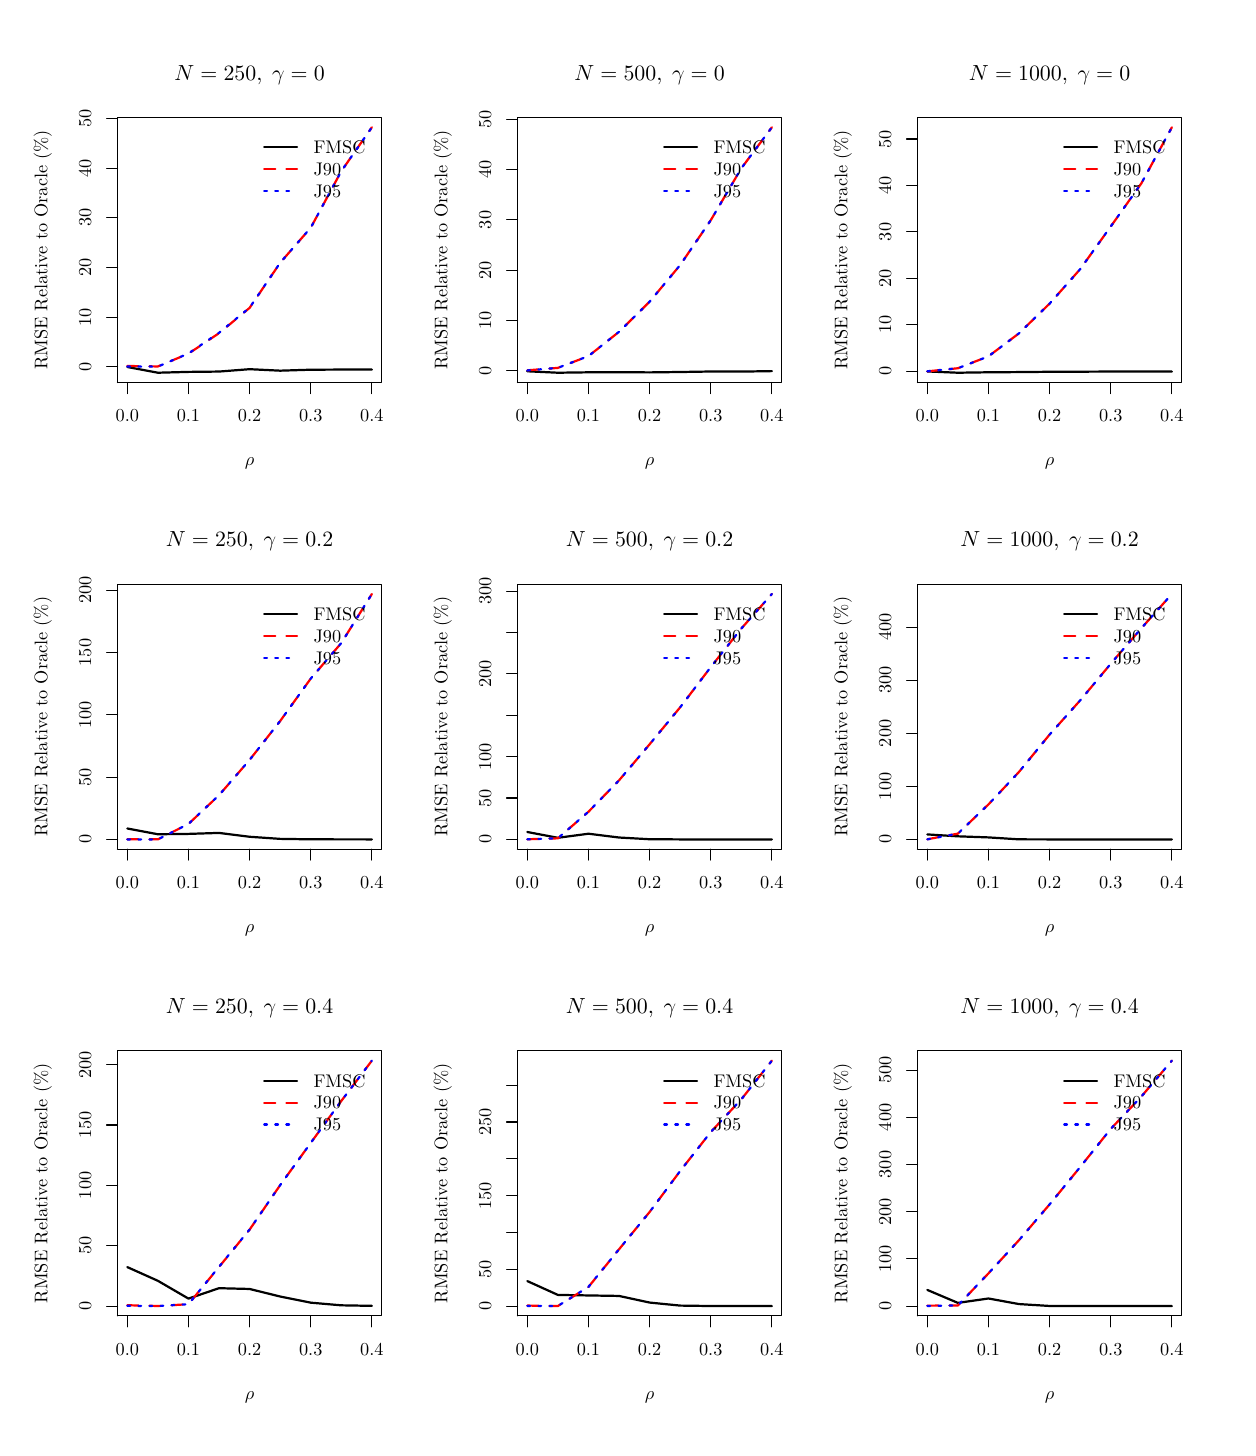
\begin{tikzpicture}[x=1pt,y=1pt]
\definecolor[named]{fillColor}{rgb}{1.00,1.00,1.00}
\path[use as bounding box,fill=fillColor,fill opacity=0.00] (0,0) rectangle (433.62,505.89);
\begin{scope}
\path[clip] ( 32.47,377.65) rectangle (127.91,473.42);
\definecolor[named]{drawColor}{rgb}{0.00,0.00,0.00}

\path[draw=drawColor,line width= 0.8pt,line join=round,line cap=round] ( 36.01,383.27) --
	( 47.05,381.20) --
	( 58.10,381.50) --
	( 69.14,381.62) --
	( 80.19,382.48) --
	( 91.24,381.94) --
	(102.28,382.29) --
	(113.33,382.34) --
	(124.37,382.35);
\end{scope}
\begin{scope}
\path[clip] (  0.00,  0.00) rectangle (433.62,505.89);
\definecolor[named]{drawColor}{rgb}{0.00,0.00,0.00}

\path[draw=drawColor,line width= 0.4pt,line join=round,line cap=round] ( 36.01,377.65) -- (124.37,377.65);

\path[draw=drawColor,line width= 0.4pt,line join=round,line cap=round] ( 36.01,377.65) -- ( 36.01,373.69);

\path[draw=drawColor,line width= 0.4pt,line join=round,line cap=round] ( 58.10,377.65) -- ( 58.10,373.69);

\path[draw=drawColor,line width= 0.4pt,line join=round,line cap=round] ( 80.19,377.65) -- ( 80.19,373.69);

\path[draw=drawColor,line width= 0.4pt,line join=round,line cap=round] (102.28,377.65) -- (102.28,373.69);

\path[draw=drawColor,line width= 0.4pt,line join=round,line cap=round] (124.37,377.65) -- (124.37,373.69);

\node[text=drawColor,anchor=base,inner sep=0pt, outer sep=0pt, scale=  0.66] at ( 36.01,363.40) {0.0};

\node[text=drawColor,anchor=base,inner sep=0pt, outer sep=0pt, scale=  0.66] at ( 58.10,363.40) {0.1};

\node[text=drawColor,anchor=base,inner sep=0pt, outer sep=0pt, scale=  0.66] at ( 80.19,363.40) {0.2};

\node[text=drawColor,anchor=base,inner sep=0pt, outer sep=0pt, scale=  0.66] at (102.28,363.40) {0.3};

\node[text=drawColor,anchor=base,inner sep=0pt, outer sep=0pt, scale=  0.66] at (124.37,363.40) {0.4};

\path[draw=drawColor,line width= 0.4pt,line join=round,line cap=round] ( 32.47,383.37) -- ( 32.47,473.05);

\path[draw=drawColor,line width= 0.4pt,line join=round,line cap=round] ( 32.47,383.37) -- ( 28.51,383.37);

\path[draw=drawColor,line width= 0.4pt,line join=round,line cap=round] ( 32.47,401.30) -- ( 28.51,401.30);

\path[draw=drawColor,line width= 0.4pt,line join=round,line cap=round] ( 32.47,419.24) -- ( 28.51,419.24);

\path[draw=drawColor,line width= 0.4pt,line join=round,line cap=round] ( 32.47,437.17) -- ( 28.51,437.17);

\path[draw=drawColor,line width= 0.4pt,line join=round,line cap=round] ( 32.47,455.11) -- ( 28.51,455.11);

\path[draw=drawColor,line width= 0.4pt,line join=round,line cap=round] ( 32.47,473.05) -- ( 28.51,473.05);

\node[text=drawColor,rotate= 90.00,anchor=base,inner sep=0pt, outer sep=0pt, scale=  0.66] at ( 22.97,383.37) {0};

\node[text=drawColor,rotate= 90.00,anchor=base,inner sep=0pt, outer sep=0pt, scale=  0.66] at ( 22.97,401.30) {10};

\node[text=drawColor,rotate= 90.00,anchor=base,inner sep=0pt, outer sep=0pt, scale=  0.66] at ( 22.97,419.24) {20};

\node[text=drawColor,rotate= 90.00,anchor=base,inner sep=0pt, outer sep=0pt, scale=  0.66] at ( 22.97,437.17) {30};

\node[text=drawColor,rotate= 90.00,anchor=base,inner sep=0pt, outer sep=0pt, scale=  0.66] at ( 22.97,455.11) {40};

\node[text=drawColor,rotate= 90.00,anchor=base,inner sep=0pt, outer sep=0pt, scale=  0.66] at ( 22.97,473.05) {50};

\path[draw=drawColor,line width= 0.4pt,line join=round,line cap=round] ( 32.47,377.65) --
	(127.91,377.65) --
	(127.91,473.42) --
	( 32.47,473.42) --
	( 32.47,377.65);
\end{scope}
\begin{scope}
\path[clip] (  0.00,337.26) rectangle (144.54,505.89);
\definecolor[named]{drawColor}{rgb}{0.00,0.00,0.00}

\node[text=drawColor,anchor=base,inner sep=0pt, outer sep=0pt, scale=  0.79] at ( 80.19,486.92) {\bfseries $N=250, \;\gamma=0$};

\node[text=drawColor,anchor=base,inner sep=0pt, outer sep=0pt, scale=  0.66] at ( 80.19,347.56) {$\rho$};

\node[text=drawColor,rotate= 90.00,anchor=base,inner sep=0pt, outer sep=0pt, scale=  0.66] at (  7.13,425.53) {RMSE Relative to Oracle (\%)};
\end{scope}
\begin{scope}
\path[clip] ( 32.47,377.65) rectangle (127.91,473.42);
\definecolor[named]{drawColor}{rgb}{1.00,0.00,0.00}

\path[draw=drawColor,line width= 0.8pt,dash pattern=on 4pt off 4pt ,line join=round,line cap=round] ( 36.01,383.63) --
	( 47.05,383.47) --
	( 58.10,388.09) --
	( 69.14,395.48) --
	( 80.19,404.63) --
	( 91.24,420.93) --
	(102.28,433.58) --
	(113.33,454.03) --
	(124.37,469.87);
\definecolor[named]{drawColor}{rgb}{0.00,0.00,1.00}

\path[draw=drawColor,line width= 0.8pt,dash pattern=on 1pt off 3pt ,line join=round,line cap=round] ( 36.01,383.42) --
	( 47.05,383.41) --
	( 58.10,388.16) --
	( 69.14,395.62) --
	( 80.19,404.69) --
	( 91.24,420.95) --
	(102.28,433.58) --
	(113.33,454.03) --
	(124.37,469.87);
\definecolor[named]{drawColor}{rgb}{0.00,0.00,0.00}

\path[draw=drawColor,line width= 0.8pt,line join=round,line cap=round] ( 85.47,462.63) -- ( 97.35,462.63);
\definecolor[named]{drawColor}{rgb}{1.00,0.00,0.00}

\path[draw=drawColor,line width= 0.8pt,dash pattern=on 4pt off 4pt ,line join=round,line cap=round] ( 85.47,454.71) -- ( 97.35,454.71);
\definecolor[named]{drawColor}{rgb}{0.00,0.00,1.00}

\path[draw=drawColor,line width= 0.8pt,dash pattern=on 1pt off 3pt ,line join=round,line cap=round] ( 85.47,446.79) -- ( 97.35,446.79);
\definecolor[named]{drawColor}{rgb}{0.00,0.00,0.00}

\node[text=drawColor,anchor=base west,inner sep=0pt, outer sep=0pt, scale=  0.66] at (103.29,460.35) {FMSC};

\node[text=drawColor,anchor=base west,inner sep=0pt, outer sep=0pt, scale=  0.66] at (103.29,452.43) {J90};

\node[text=drawColor,anchor=base west,inner sep=0pt, outer sep=0pt, scale=  0.66] at (103.29,444.51) {J95};
\end{scope}
\begin{scope}
\path[clip] (177.01,377.65) rectangle (272.45,473.42);
\definecolor[named]{drawColor}{rgb}{0.00,0.00,0.00}

\path[draw=drawColor,line width= 0.8pt,line join=round,line cap=round] (180.55,381.72) --
	(191.59,381.20) --
	(202.64,381.35) --
	(213.68,381.40) --
	(224.73,381.32) --
	(235.78,381.46) --
	(246.82,381.64) --
	(257.87,381.61) --
	(268.91,381.78);
\end{scope}
\begin{scope}
\path[clip] (  0.00,  0.00) rectangle (433.62,505.89);
\definecolor[named]{drawColor}{rgb}{0.00,0.00,0.00}

\path[draw=drawColor,line width= 0.4pt,line join=round,line cap=round] (180.55,377.65) -- (268.91,377.65);

\path[draw=drawColor,line width= 0.4pt,line join=round,line cap=round] (180.55,377.65) -- (180.55,373.69);

\path[draw=drawColor,line width= 0.4pt,line join=round,line cap=round] (202.64,377.65) -- (202.64,373.69);

\path[draw=drawColor,line width= 0.4pt,line join=round,line cap=round] (224.73,377.65) -- (224.73,373.69);

\path[draw=drawColor,line width= 0.4pt,line join=round,line cap=round] (246.82,377.65) -- (246.82,373.69);

\path[draw=drawColor,line width= 0.4pt,line join=round,line cap=round] (268.91,377.65) -- (268.91,373.69);

\node[text=drawColor,anchor=base,inner sep=0pt, outer sep=0pt, scale=  0.66] at (180.55,363.40) {0.0};

\node[text=drawColor,anchor=base,inner sep=0pt, outer sep=0pt, scale=  0.66] at (202.64,363.40) {0.1};

\node[text=drawColor,anchor=base,inner sep=0pt, outer sep=0pt, scale=  0.66] at (224.73,363.40) {0.2};

\node[text=drawColor,anchor=base,inner sep=0pt, outer sep=0pt, scale=  0.66] at (246.82,363.40) {0.3};

\node[text=drawColor,anchor=base,inner sep=0pt, outer sep=0pt, scale=  0.66] at (268.91,363.40) {0.4};

\path[draw=drawColor,line width= 0.4pt,line join=round,line cap=round] (177.01,382.01) -- (177.01,472.72);

\path[draw=drawColor,line width= 0.4pt,line join=round,line cap=round] (177.01,382.01) -- (173.05,382.01);

\path[draw=drawColor,line width= 0.4pt,line join=round,line cap=round] (177.01,400.15) -- (173.05,400.15);

\path[draw=drawColor,line width= 0.4pt,line join=round,line cap=round] (177.01,418.29) -- (173.05,418.29);

\path[draw=drawColor,line width= 0.4pt,line join=round,line cap=round] (177.01,436.43) -- (173.05,436.43);

\path[draw=drawColor,line width= 0.4pt,line join=round,line cap=round] (177.01,454.58) -- (173.05,454.58);

\path[draw=drawColor,line width= 0.4pt,line join=round,line cap=round] (177.01,472.72) -- (173.05,472.72);

\node[text=drawColor,rotate= 90.00,anchor=base,inner sep=0pt, outer sep=0pt, scale=  0.66] at (167.51,382.01) {0};

\node[text=drawColor,rotate= 90.00,anchor=base,inner sep=0pt, outer sep=0pt, scale=  0.66] at (167.51,400.15) {10};

\node[text=drawColor,rotate= 90.00,anchor=base,inner sep=0pt, outer sep=0pt, scale=  0.66] at (167.51,418.29) {20};

\node[text=drawColor,rotate= 90.00,anchor=base,inner sep=0pt, outer sep=0pt, scale=  0.66] at (167.51,436.43) {30};

\node[text=drawColor,rotate= 90.00,anchor=base,inner sep=0pt, outer sep=0pt, scale=  0.66] at (167.51,454.58) {40};

\node[text=drawColor,rotate= 90.00,anchor=base,inner sep=0pt, outer sep=0pt, scale=  0.66] at (167.51,472.72) {50};

\path[draw=drawColor,line width= 0.4pt,line join=round,line cap=round] (177.01,377.65) --
	(272.45,377.65) --
	(272.45,473.42) --
	(177.01,473.42) --
	(177.01,377.65);
\end{scope}
\begin{scope}
\path[clip] (144.54,337.26) rectangle (289.08,505.89);
\definecolor[named]{drawColor}{rgb}{0.00,0.00,0.00}

\node[text=drawColor,anchor=base,inner sep=0pt, outer sep=0pt, scale=  0.79] at (224.73,486.92) {\bfseries $N=500, \;\gamma=0$};

\node[text=drawColor,anchor=base,inner sep=0pt, outer sep=0pt, scale=  0.66] at (224.73,347.56) {$\rho$};

\node[text=drawColor,rotate= 90.00,anchor=base,inner sep=0pt, outer sep=0pt, scale=  0.66] at (151.67,425.53) {RMSE Relative to Oracle (\%)};
\end{scope}
\begin{scope}
\path[clip] (177.01,377.65) rectangle (272.45,473.42);
\definecolor[named]{drawColor}{rgb}{1.00,0.00,0.00}

\path[draw=drawColor,line width= 0.8pt,dash pattern=on 4pt off 4pt ,line join=round,line cap=round] (180.55,382.07) --
	(191.59,382.95) --
	(202.64,387.20) --
	(213.68,395.98) --
	(224.73,406.86) --
	(235.78,420.12) --
	(246.82,436.29) --
	(257.87,455.07) --
	(268.91,469.87);
\definecolor[named]{drawColor}{rgb}{0.00,0.00,1.00}

\path[draw=drawColor,line width= 0.8pt,dash pattern=on 1pt off 3pt ,line join=round,line cap=round] (180.55,382.02) --
	(191.59,382.96) --
	(202.64,387.22) --
	(213.68,395.98) --
	(224.73,406.86) --
	(235.78,420.12) --
	(246.82,436.29) --
	(257.87,455.07) --
	(268.91,469.87);
\definecolor[named]{drawColor}{rgb}{0.00,0.00,0.00}

\path[draw=drawColor,line width= 0.8pt,line join=round,line cap=round] (230.01,462.63) -- (241.89,462.63);
\definecolor[named]{drawColor}{rgb}{1.00,0.00,0.00}

\path[draw=drawColor,line width= 0.8pt,dash pattern=on 4pt off 4pt ,line join=round,line cap=round] (230.01,454.71) -- (241.89,454.71);
\definecolor[named]{drawColor}{rgb}{0.00,0.00,1.00}

\path[draw=drawColor,line width= 0.8pt,dash pattern=on 1pt off 3pt ,line join=round,line cap=round] (230.01,446.79) -- (241.89,446.79);
\definecolor[named]{drawColor}{rgb}{0.00,0.00,0.00}

\node[text=drawColor,anchor=base west,inner sep=0pt, outer sep=0pt, scale=  0.66] at (247.83,460.35) {FMSC};

\node[text=drawColor,anchor=base west,inner sep=0pt, outer sep=0pt, scale=  0.66] at (247.83,452.43) {J90};

\node[text=drawColor,anchor=base west,inner sep=0pt, outer sep=0pt, scale=  0.66] at (247.83,444.51) {J95};
\end{scope}
\begin{scope}
\path[clip] (321.55,377.65) rectangle (416.99,473.42);
\definecolor[named]{drawColor}{rgb}{0.00,0.00,0.00}

\path[draw=drawColor,line width= 0.8pt,line join=round,line cap=round] (325.09,381.66) --
	(336.13,381.20) --
	(347.18,381.36) --
	(358.22,381.43) --
	(369.27,381.54) --
	(380.32,381.58) --
	(391.36,381.62) --
	(402.41,381.61) --
	(413.45,381.61);
\end{scope}
\begin{scope}
\path[clip] (  0.00,  0.00) rectangle (433.62,505.89);
\definecolor[named]{drawColor}{rgb}{0.00,0.00,0.00}

\path[draw=drawColor,line width= 0.4pt,line join=round,line cap=round] (325.09,377.65) -- (413.45,377.65);

\path[draw=drawColor,line width= 0.4pt,line join=round,line cap=round] (325.09,377.65) -- (325.09,373.69);

\path[draw=drawColor,line width= 0.4pt,line join=round,line cap=round] (347.18,377.65) -- (347.18,373.69);

\path[draw=drawColor,line width= 0.4pt,line join=round,line cap=round] (369.27,377.65) -- (369.27,373.69);

\path[draw=drawColor,line width= 0.4pt,line join=round,line cap=round] (391.36,377.65) -- (391.36,373.69);

\path[draw=drawColor,line width= 0.4pt,line join=round,line cap=round] (413.45,377.65) -- (413.45,373.69);

\node[text=drawColor,anchor=base,inner sep=0pt, outer sep=0pt, scale=  0.66] at (325.09,363.40) {0.0};

\node[text=drawColor,anchor=base,inner sep=0pt, outer sep=0pt, scale=  0.66] at (347.18,363.40) {0.1};

\node[text=drawColor,anchor=base,inner sep=0pt, outer sep=0pt, scale=  0.66] at (369.27,363.40) {0.2};

\node[text=drawColor,anchor=base,inner sep=0pt, outer sep=0pt, scale=  0.66] at (391.36,363.40) {0.3};

\node[text=drawColor,anchor=base,inner sep=0pt, outer sep=0pt, scale=  0.66] at (413.45,363.40) {0.4};

\path[draw=drawColor,line width= 0.4pt,line join=round,line cap=round] (321.55,381.72) -- (321.55,465.64);

\path[draw=drawColor,line width= 0.4pt,line join=round,line cap=round] (321.55,381.72) -- (317.59,381.72);

\path[draw=drawColor,line width= 0.4pt,line join=round,line cap=round] (321.55,398.50) -- (317.59,398.50);

\path[draw=drawColor,line width= 0.4pt,line join=round,line cap=round] (321.55,415.28) -- (317.59,415.28);

\path[draw=drawColor,line width= 0.4pt,line join=round,line cap=round] (321.55,432.07) -- (317.59,432.07);

\path[draw=drawColor,line width= 0.4pt,line join=round,line cap=round] (321.55,448.85) -- (317.59,448.85);

\path[draw=drawColor,line width= 0.4pt,line join=round,line cap=round] (321.55,465.64) -- (317.59,465.64);

\node[text=drawColor,rotate= 90.00,anchor=base,inner sep=0pt, outer sep=0pt, scale=  0.66] at (312.05,381.72) {0};

\node[text=drawColor,rotate= 90.00,anchor=base,inner sep=0pt, outer sep=0pt, scale=  0.66] at (312.05,398.50) {10};

\node[text=drawColor,rotate= 90.00,anchor=base,inner sep=0pt, outer sep=0pt, scale=  0.66] at (312.05,415.28) {20};

\node[text=drawColor,rotate= 90.00,anchor=base,inner sep=0pt, outer sep=0pt, scale=  0.66] at (312.05,432.07) {30};

\node[text=drawColor,rotate= 90.00,anchor=base,inner sep=0pt, outer sep=0pt, scale=  0.66] at (312.05,448.85) {40};

\node[text=drawColor,rotate= 90.00,anchor=base,inner sep=0pt, outer sep=0pt, scale=  0.66] at (312.05,465.64) {50};

\path[draw=drawColor,line width= 0.4pt,line join=round,line cap=round] (321.55,377.65) --
	(416.99,377.65) --
	(416.99,473.42) --
	(321.55,473.42) --
	(321.55,377.65);
\end{scope}
\begin{scope}
\path[clip] (289.08,337.26) rectangle (433.62,505.89);
\definecolor[named]{drawColor}{rgb}{0.00,0.00,0.00}

\node[text=drawColor,anchor=base,inner sep=0pt, outer sep=0pt, scale=  0.79] at (369.27,486.92) {\bfseries $N=1000, \;\gamma=0$};

\node[text=drawColor,anchor=base,inner sep=0pt, outer sep=0pt, scale=  0.66] at (369.27,347.56) {$\rho$};

\node[text=drawColor,rotate= 90.00,anchor=base,inner sep=0pt, outer sep=0pt, scale=  0.66] at (296.21,425.53) {RMSE Relative to Oracle (\%)};
\end{scope}
\begin{scope}
\path[clip] (321.55,377.65) rectangle (416.99,473.42);
\definecolor[named]{drawColor}{rgb}{1.00,0.00,0.00}

\path[draw=drawColor,line width= 0.8pt,dash pattern=on 4pt off 4pt ,line join=round,line cap=round] (325.09,381.70) --
	(336.13,382.82) --
	(347.18,387.12) --
	(358.22,395.44) --
	(369.27,406.17) --
	(380.32,418.63) --
	(391.36,434.03) --
	(402.41,449.60) --
	(413.45,469.87);
\definecolor[named]{drawColor}{rgb}{0.00,0.00,1.00}

\path[draw=drawColor,line width= 0.8pt,dash pattern=on 1pt off 3pt ,line join=round,line cap=round] (325.09,381.72) --
	(336.13,382.82) --
	(347.18,387.12) --
	(358.22,395.44) --
	(369.27,406.17) --
	(380.32,418.63) --
	(391.36,434.03) --
	(402.41,449.60) --
	(413.45,469.87);
\definecolor[named]{drawColor}{rgb}{0.00,0.00,0.00}

\path[draw=drawColor,line width= 0.8pt,line join=round,line cap=round] (374.55,462.63) -- (386.43,462.63);
\definecolor[named]{drawColor}{rgb}{1.00,0.00,0.00}

\path[draw=drawColor,line width= 0.8pt,dash pattern=on 4pt off 4pt ,line join=round,line cap=round] (374.55,454.71) -- (386.43,454.71);
\definecolor[named]{drawColor}{rgb}{0.00,0.00,1.00}

\path[draw=drawColor,line width= 0.8pt,dash pattern=on 1pt off 3pt ,line join=round,line cap=round] (374.55,446.79) -- (386.43,446.79);
\definecolor[named]{drawColor}{rgb}{0.00,0.00,0.00}

\node[text=drawColor,anchor=base west,inner sep=0pt, outer sep=0pt, scale=  0.66] at (392.37,460.35) {FMSC};

\node[text=drawColor,anchor=base west,inner sep=0pt, outer sep=0pt, scale=  0.66] at (392.37,452.43) {J90};

\node[text=drawColor,anchor=base west,inner sep=0pt, outer sep=0pt, scale=  0.66] at (392.37,444.51) {J95};
\end{scope}
\begin{scope}
\path[clip] ( 32.47,209.02) rectangle (127.91,304.79);
\definecolor[named]{drawColor}{rgb}{0.00,0.00,0.00}

\path[draw=drawColor,line width= 0.8pt,line join=round,line cap=round] ( 36.01,216.51) --
	( 47.05,214.43) --
	( 58.10,214.56) --
	( 69.14,214.91) --
	( 80.19,213.52) --
	( 91.24,212.76) --
	(102.28,212.60) --
	(113.33,212.58) --
	(124.37,212.57);
\end{scope}
\begin{scope}
\path[clip] (  0.00,  0.00) rectangle (433.62,505.89);
\definecolor[named]{drawColor}{rgb}{0.00,0.00,0.00}

\path[draw=drawColor,line width= 0.4pt,line join=round,line cap=round] ( 36.01,209.02) -- (124.37,209.02);

\path[draw=drawColor,line width= 0.4pt,line join=round,line cap=round] ( 36.01,209.02) -- ( 36.01,205.06);

\path[draw=drawColor,line width= 0.4pt,line join=round,line cap=round] ( 58.10,209.02) -- ( 58.10,205.06);

\path[draw=drawColor,line width= 0.4pt,line join=round,line cap=round] ( 80.19,209.02) -- ( 80.19,205.06);

\path[draw=drawColor,line width= 0.4pt,line join=round,line cap=round] (102.28,209.02) -- (102.28,205.06);

\path[draw=drawColor,line width= 0.4pt,line join=round,line cap=round] (124.37,209.02) -- (124.37,205.06);

\node[text=drawColor,anchor=base,inner sep=0pt, outer sep=0pt, scale=  0.66] at ( 36.01,194.77) {0.0};

\node[text=drawColor,anchor=base,inner sep=0pt, outer sep=0pt, scale=  0.66] at ( 58.10,194.77) {0.1};

\node[text=drawColor,anchor=base,inner sep=0pt, outer sep=0pt, scale=  0.66] at ( 80.19,194.77) {0.2};

\node[text=drawColor,anchor=base,inner sep=0pt, outer sep=0pt, scale=  0.66] at (102.28,194.77) {0.3};

\node[text=drawColor,anchor=base,inner sep=0pt, outer sep=0pt, scale=  0.66] at (124.37,194.77) {0.4};

\path[draw=drawColor,line width= 0.4pt,line join=round,line cap=round] ( 32.47,212.57) -- ( 32.47,302.60);

\path[draw=drawColor,line width= 0.4pt,line join=round,line cap=round] ( 32.47,212.57) -- ( 28.51,212.57);

\path[draw=drawColor,line width= 0.4pt,line join=round,line cap=round] ( 32.47,235.08) -- ( 28.51,235.08);

\path[draw=drawColor,line width= 0.4pt,line join=round,line cap=round] ( 32.47,257.59) -- ( 28.51,257.59);

\path[draw=drawColor,line width= 0.4pt,line join=round,line cap=round] ( 32.47,280.09) -- ( 28.51,280.09);

\path[draw=drawColor,line width= 0.4pt,line join=round,line cap=round] ( 32.47,302.60) -- ( 28.51,302.60);

\node[text=drawColor,rotate= 90.00,anchor=base,inner sep=0pt, outer sep=0pt, scale=  0.66] at ( 22.97,212.57) {0};

\node[text=drawColor,rotate= 90.00,anchor=base,inner sep=0pt, outer sep=0pt, scale=  0.66] at ( 22.97,235.08) {50};

\node[text=drawColor,rotate= 90.00,anchor=base,inner sep=0pt, outer sep=0pt, scale=  0.66] at ( 22.97,257.59) {100};

\node[text=drawColor,rotate= 90.00,anchor=base,inner sep=0pt, outer sep=0pt, scale=  0.66] at ( 22.97,280.09) {150};

\node[text=drawColor,rotate= 90.00,anchor=base,inner sep=0pt, outer sep=0pt, scale=  0.66] at ( 22.97,302.60) {200};

\path[draw=drawColor,line width= 0.4pt,line join=round,line cap=round] ( 32.47,209.02) --
	(127.91,209.02) --
	(127.91,304.79) --
	( 32.47,304.79) --
	( 32.47,209.02);
\end{scope}
\begin{scope}
\path[clip] (  0.00,168.63) rectangle (144.54,337.26);
\definecolor[named]{drawColor}{rgb}{0.00,0.00,0.00}

\node[text=drawColor,anchor=base,inner sep=0pt, outer sep=0pt, scale=  0.79] at ( 80.19,318.29) {\bfseries $N=250, \;\gamma=0.2$};

\node[text=drawColor,anchor=base,inner sep=0pt, outer sep=0pt, scale=  0.66] at ( 80.19,178.93) {$\rho$};

\node[text=drawColor,rotate= 90.00,anchor=base,inner sep=0pt, outer sep=0pt, scale=  0.66] at (  7.13,256.90) {RMSE Relative to Oracle (\%)};
\end{scope}
\begin{scope}
\path[clip] ( 32.47,209.02) rectangle (127.91,304.79);
\definecolor[named]{drawColor}{rgb}{1.00,0.00,0.00}

\path[draw=drawColor,line width= 0.8pt,dash pattern=on 4pt off 4pt ,line join=round,line cap=round] ( 36.01,212.63) --
	( 47.05,212.59) --
	( 58.10,218.14) --
	( 69.14,228.53) --
	( 80.19,241.29) --
	( 91.24,255.35) --
	(102.28,270.67) --
	(113.33,283.53) --
	(124.37,301.24);
\definecolor[named]{drawColor}{rgb}{0.00,0.00,1.00}

\path[draw=drawColor,line width= 0.8pt,dash pattern=on 1pt off 3pt ,line join=round,line cap=round] ( 36.01,212.57) --
	( 47.05,212.57) --
	( 58.10,218.15) --
	( 69.14,228.55) --
	( 80.19,241.30) --
	( 91.24,255.35) --
	(102.28,270.67) --
	(113.33,283.53) --
	(124.37,301.24);
\definecolor[named]{drawColor}{rgb}{0.00,0.00,0.00}

\path[draw=drawColor,line width= 0.8pt,line join=round,line cap=round] ( 85.47,294.00) -- ( 97.35,294.00);
\definecolor[named]{drawColor}{rgb}{1.00,0.00,0.00}

\path[draw=drawColor,line width= 0.8pt,dash pattern=on 4pt off 4pt ,line join=round,line cap=round] ( 85.47,286.08) -- ( 97.35,286.08);
\definecolor[named]{drawColor}{rgb}{0.00,0.00,1.00}

\path[draw=drawColor,line width= 0.8pt,dash pattern=on 1pt off 3pt ,line join=round,line cap=round] ( 85.47,278.16) -- ( 97.35,278.16);
\definecolor[named]{drawColor}{rgb}{0.00,0.00,0.00}

\node[text=drawColor,anchor=base west,inner sep=0pt, outer sep=0pt, scale=  0.66] at (103.29,291.72) {FMSC};

\node[text=drawColor,anchor=base west,inner sep=0pt, outer sep=0pt, scale=  0.66] at (103.29,283.80) {J90};

\node[text=drawColor,anchor=base west,inner sep=0pt, outer sep=0pt, scale=  0.66] at (103.29,275.88) {J95};
\end{scope}
\begin{scope}
\path[clip] (177.01,209.02) rectangle (272.45,304.79);
\definecolor[named]{drawColor}{rgb}{0.00,0.00,0.00}

\path[draw=drawColor,line width= 0.8pt,line join=round,line cap=round] (180.55,215.24) --
	(191.59,213.15) --
	(202.64,214.62) --
	(213.68,213.25) --
	(224.73,212.63) --
	(235.78,212.57) --
	(246.82,212.57) --
	(257.87,212.57) --
	(268.91,212.57);
\end{scope}
\begin{scope}
\path[clip] (  0.00,  0.00) rectangle (433.62,505.89);
\definecolor[named]{drawColor}{rgb}{0.00,0.00,0.00}

\path[draw=drawColor,line width= 0.4pt,line join=round,line cap=round] (180.55,209.02) -- (268.91,209.02);

\path[draw=drawColor,line width= 0.4pt,line join=round,line cap=round] (180.55,209.02) -- (180.55,205.06);

\path[draw=drawColor,line width= 0.4pt,line join=round,line cap=round] (202.64,209.02) -- (202.64,205.06);

\path[draw=drawColor,line width= 0.4pt,line join=round,line cap=round] (224.73,209.02) -- (224.73,205.06);

\path[draw=drawColor,line width= 0.4pt,line join=round,line cap=round] (246.82,209.02) -- (246.82,205.06);

\path[draw=drawColor,line width= 0.4pt,line join=round,line cap=round] (268.91,209.02) -- (268.91,205.06);

\node[text=drawColor,anchor=base,inner sep=0pt, outer sep=0pt, scale=  0.66] at (180.55,194.77) {0.0};

\node[text=drawColor,anchor=base,inner sep=0pt, outer sep=0pt, scale=  0.66] at (202.64,194.77) {0.1};

\node[text=drawColor,anchor=base,inner sep=0pt, outer sep=0pt, scale=  0.66] at (224.73,194.77) {0.2};

\node[text=drawColor,anchor=base,inner sep=0pt, outer sep=0pt, scale=  0.66] at (246.82,194.77) {0.3};

\node[text=drawColor,anchor=base,inner sep=0pt, outer sep=0pt, scale=  0.66] at (268.91,194.77) {0.4};

\path[draw=drawColor,line width= 0.4pt,line join=round,line cap=round] (177.01,212.57) -- (177.01,302.27);

\path[draw=drawColor,line width= 0.4pt,line join=round,line cap=round] (177.01,212.57) -- (173.05,212.57);

\path[draw=drawColor,line width= 0.4pt,line join=round,line cap=round] (177.01,227.52) -- (173.05,227.52);

\path[draw=drawColor,line width= 0.4pt,line join=round,line cap=round] (177.01,242.47) -- (173.05,242.47);

\path[draw=drawColor,line width= 0.4pt,line join=round,line cap=round] (177.01,257.42) -- (173.05,257.42);

\path[draw=drawColor,line width= 0.4pt,line join=round,line cap=round] (177.01,272.37) -- (173.05,272.37);

\path[draw=drawColor,line width= 0.4pt,line join=round,line cap=round] (177.01,287.32) -- (173.05,287.32);

\path[draw=drawColor,line width= 0.4pt,line join=round,line cap=round] (177.01,302.27) -- (173.05,302.27);

\node[text=drawColor,rotate= 90.00,anchor=base,inner sep=0pt, outer sep=0pt, scale=  0.66] at (167.51,212.57) {0};

\node[text=drawColor,rotate= 90.00,anchor=base,inner sep=0pt, outer sep=0pt, scale=  0.66] at (167.51,227.52) {50};

\node[text=drawColor,rotate= 90.00,anchor=base,inner sep=0pt, outer sep=0pt, scale=  0.66] at (167.51,242.47) {100};

\node[text=drawColor,rotate= 90.00,anchor=base,inner sep=0pt, outer sep=0pt, scale=  0.66] at (167.51,272.37) {200};

\node[text=drawColor,rotate= 90.00,anchor=base,inner sep=0pt, outer sep=0pt, scale=  0.66] at (167.51,302.27) {300};

\path[draw=drawColor,line width= 0.4pt,line join=round,line cap=round] (177.01,209.02) --
	(272.45,209.02) --
	(272.45,304.79) --
	(177.01,304.79) --
	(177.01,209.02);
\end{scope}
\begin{scope}
\path[clip] (144.54,168.63) rectangle (289.08,337.26);
\definecolor[named]{drawColor}{rgb}{0.00,0.00,0.00}

\node[text=drawColor,anchor=base,inner sep=0pt, outer sep=0pt, scale=  0.79] at (224.73,318.29) {\bfseries $N=500, \;\gamma=0.2$};

\node[text=drawColor,anchor=base,inner sep=0pt, outer sep=0pt, scale=  0.66] at (224.73,178.93) {$\rho$};

\node[text=drawColor,rotate= 90.00,anchor=base,inner sep=0pt, outer sep=0pt, scale=  0.66] at (151.67,256.90) {RMSE Relative to Oracle (\%)};
\end{scope}
\begin{scope}
\path[clip] (177.01,209.02) rectangle (272.45,304.79);
\definecolor[named]{drawColor}{rgb}{1.00,0.00,0.00}

\path[draw=drawColor,line width= 0.8pt,dash pattern=on 4pt off 4pt ,line join=round,line cap=round] (180.55,212.62) --
	(191.59,212.96) --
	(202.64,222.56) --
	(213.68,233.90) --
	(224.73,246.93) --
	(235.78,260.31) --
	(246.82,274.82) --
	(257.87,288.76) --
	(268.91,301.24);
\definecolor[named]{drawColor}{rgb}{0.00,0.00,1.00}

\path[draw=drawColor,line width= 0.8pt,dash pattern=on 1pt off 3pt ,line join=round,line cap=round] (180.55,212.60) --
	(191.59,212.98) --
	(202.64,222.57) --
	(213.68,233.90) --
	(224.73,246.93) --
	(235.78,260.31) --
	(246.82,274.82) --
	(257.87,288.76) --
	(268.91,301.24);
\definecolor[named]{drawColor}{rgb}{0.00,0.00,0.00}

\path[draw=drawColor,line width= 0.8pt,line join=round,line cap=round] (230.01,294.00) -- (241.89,294.00);
\definecolor[named]{drawColor}{rgb}{1.00,0.00,0.00}

\path[draw=drawColor,line width= 0.8pt,dash pattern=on 4pt off 4pt ,line join=round,line cap=round] (230.01,286.08) -- (241.89,286.08);
\definecolor[named]{drawColor}{rgb}{0.00,0.00,1.00}

\path[draw=drawColor,line width= 0.8pt,dash pattern=on 1pt off 3pt ,line join=round,line cap=round] (230.01,278.16) -- (241.89,278.16);
\definecolor[named]{drawColor}{rgb}{0.00,0.00,0.00}

\node[text=drawColor,anchor=base west,inner sep=0pt, outer sep=0pt, scale=  0.66] at (247.83,291.72) {FMSC};

\node[text=drawColor,anchor=base west,inner sep=0pt, outer sep=0pt, scale=  0.66] at (247.83,283.80) {J90};

\node[text=drawColor,anchor=base west,inner sep=0pt, outer sep=0pt, scale=  0.66] at (247.83,275.88) {J95};
\end{scope}
\begin{scope}
\path[clip] (321.55,209.02) rectangle (416.99,304.79);
\definecolor[named]{drawColor}{rgb}{0.00,0.00,0.00}

\path[draw=drawColor,line width= 0.8pt,line join=round,line cap=round] (325.09,214.37) --
	(336.13,213.68) --
	(347.18,213.29) --
	(358.22,212.59) --
	(369.27,212.57) --
	(380.32,212.57) --
	(391.36,212.57) --
	(402.41,212.57) --
	(413.45,212.57);
\end{scope}
\begin{scope}
\path[clip] (  0.00,  0.00) rectangle (433.62,505.89);
\definecolor[named]{drawColor}{rgb}{0.00,0.00,0.00}

\path[draw=drawColor,line width= 0.4pt,line join=round,line cap=round] (325.09,209.02) -- (413.45,209.02);

\path[draw=drawColor,line width= 0.4pt,line join=round,line cap=round] (325.09,209.02) -- (325.09,205.06);

\path[draw=drawColor,line width= 0.4pt,line join=round,line cap=round] (347.18,209.02) -- (347.18,205.06);

\path[draw=drawColor,line width= 0.4pt,line join=round,line cap=round] (369.27,209.02) -- (369.27,205.06);

\path[draw=drawColor,line width= 0.4pt,line join=round,line cap=round] (391.36,209.02) -- (391.36,205.06);

\path[draw=drawColor,line width= 0.4pt,line join=round,line cap=round] (413.45,209.02) -- (413.45,205.06);

\node[text=drawColor,anchor=base,inner sep=0pt, outer sep=0pt, scale=  0.66] at (325.09,194.77) {0.0};

\node[text=drawColor,anchor=base,inner sep=0pt, outer sep=0pt, scale=  0.66] at (347.18,194.77) {0.1};

\node[text=drawColor,anchor=base,inner sep=0pt, outer sep=0pt, scale=  0.66] at (369.27,194.77) {0.2};

\node[text=drawColor,anchor=base,inner sep=0pt, outer sep=0pt, scale=  0.66] at (391.36,194.77) {0.3};

\node[text=drawColor,anchor=base,inner sep=0pt, outer sep=0pt, scale=  0.66] at (413.45,194.77) {0.4};

\path[draw=drawColor,line width= 0.4pt,line join=round,line cap=round] (321.55,212.57) -- (321.55,289.25);

\path[draw=drawColor,line width= 0.4pt,line join=round,line cap=round] (321.55,212.57) -- (317.59,212.57);

\path[draw=drawColor,line width= 0.4pt,line join=round,line cap=round] (321.55,231.74) -- (317.59,231.74);

\path[draw=drawColor,line width= 0.4pt,line join=round,line cap=round] (321.55,250.91) -- (317.59,250.91);

\path[draw=drawColor,line width= 0.4pt,line join=round,line cap=round] (321.55,270.08) -- (317.59,270.08);

\path[draw=drawColor,line width= 0.4pt,line join=round,line cap=round] (321.55,289.25) -- (317.59,289.25);

\node[text=drawColor,rotate= 90.00,anchor=base,inner sep=0pt, outer sep=0pt, scale=  0.66] at (312.05,212.57) {0};

\node[text=drawColor,rotate= 90.00,anchor=base,inner sep=0pt, outer sep=0pt, scale=  0.66] at (312.05,231.74) {100};

\node[text=drawColor,rotate= 90.00,anchor=base,inner sep=0pt, outer sep=0pt, scale=  0.66] at (312.05,250.91) {200};

\node[text=drawColor,rotate= 90.00,anchor=base,inner sep=0pt, outer sep=0pt, scale=  0.66] at (312.05,270.08) {300};

\node[text=drawColor,rotate= 90.00,anchor=base,inner sep=0pt, outer sep=0pt, scale=  0.66] at (312.05,289.25) {400};

\path[draw=drawColor,line width= 0.4pt,line join=round,line cap=round] (321.55,209.02) --
	(416.99,209.02) --
	(416.99,304.79) --
	(321.55,304.79) --
	(321.55,209.02);
\end{scope}
\begin{scope}
\path[clip] (289.08,168.63) rectangle (433.62,337.26);
\definecolor[named]{drawColor}{rgb}{0.00,0.00,0.00}

\node[text=drawColor,anchor=base,inner sep=0pt, outer sep=0pt, scale=  0.79] at (369.27,318.29) {\bfseries $N=1000, \;\gamma=0.2$};

\node[text=drawColor,anchor=base,inner sep=0pt, outer sep=0pt, scale=  0.66] at (369.27,178.93) {$\rho$};

\node[text=drawColor,rotate= 90.00,anchor=base,inner sep=0pt, outer sep=0pt, scale=  0.66] at (296.21,256.90) {RMSE Relative to Oracle (\%)};
\end{scope}
\begin{scope}
\path[clip] (321.55,209.02) rectangle (416.99,304.79);
\definecolor[named]{drawColor}{rgb}{1.00,0.00,0.00}

\path[draw=drawColor,line width= 0.8pt,dash pattern=on 4pt off 4pt ,line join=round,line cap=round] (325.09,212.63) --
	(336.13,214.65) --
	(347.18,225.21) --
	(358.22,236.96) --
	(369.27,250.45) --
	(380.32,262.80) --
	(391.36,276.03) --
	(402.41,288.85) --
	(413.45,301.24);
\definecolor[named]{drawColor}{rgb}{0.00,0.00,1.00}

\path[draw=drawColor,line width= 0.8pt,dash pattern=on 1pt off 3pt ,line join=round,line cap=round] (325.09,212.58) --
	(336.13,214.66) --
	(347.18,225.22) --
	(358.22,236.96) --
	(369.27,250.45) --
	(380.32,262.80) --
	(391.36,276.03) --
	(402.41,288.85) --
	(413.45,301.24);
\definecolor[named]{drawColor}{rgb}{0.00,0.00,0.00}

\path[draw=drawColor,line width= 0.8pt,line join=round,line cap=round] (374.55,294.00) -- (386.43,294.00);
\definecolor[named]{drawColor}{rgb}{1.00,0.00,0.00}

\path[draw=drawColor,line width= 0.8pt,dash pattern=on 4pt off 4pt ,line join=round,line cap=round] (374.55,286.08) -- (386.43,286.08);
\definecolor[named]{drawColor}{rgb}{0.00,0.00,1.00}

\path[draw=drawColor,line width= 0.8pt,dash pattern=on 1pt off 3pt ,line join=round,line cap=round] (374.55,278.16) -- (386.43,278.16);
\definecolor[named]{drawColor}{rgb}{0.00,0.00,0.00}

\node[text=drawColor,anchor=base west,inner sep=0pt, outer sep=0pt, scale=  0.66] at (392.37,291.72) {FMSC};

\node[text=drawColor,anchor=base west,inner sep=0pt, outer sep=0pt, scale=  0.66] at (392.37,283.80) {J90};

\node[text=drawColor,anchor=base west,inner sep=0pt, outer sep=0pt, scale=  0.66] at (392.37,275.88) {J95};
\end{scope}
\begin{scope}
\path[clip] ( 32.47, 40.39) rectangle (127.91,136.16);
\definecolor[named]{drawColor}{rgb}{0.00,0.00,0.00}

\path[draw=drawColor,line width= 0.8pt,line join=round,line cap=round] ( 36.01, 58.02) --
	( 47.05, 53.07) --
	( 58.10, 46.64) --
	( 69.14, 50.40) --
	( 80.19, 50.12) --
	( 91.24, 47.39) --
	(102.28, 45.17) --
	(113.33, 44.21) --
	(124.37, 44.02);
\end{scope}
\begin{scope}
\path[clip] (  0.00,  0.00) rectangle (433.62,505.89);
\definecolor[named]{drawColor}{rgb}{0.00,0.00,0.00}

\path[draw=drawColor,line width= 0.4pt,line join=round,line cap=round] ( 36.01, 40.39) -- (124.37, 40.39);

\path[draw=drawColor,line width= 0.4pt,line join=round,line cap=round] ( 36.01, 40.39) -- ( 36.01, 36.43);

\path[draw=drawColor,line width= 0.4pt,line join=round,line cap=round] ( 58.10, 40.39) -- ( 58.10, 36.43);

\path[draw=drawColor,line width= 0.4pt,line join=round,line cap=round] ( 80.19, 40.39) -- ( 80.19, 36.43);

\path[draw=drawColor,line width= 0.4pt,line join=round,line cap=round] (102.28, 40.39) -- (102.28, 36.43);

\path[draw=drawColor,line width= 0.4pt,line join=round,line cap=round] (124.37, 40.39) -- (124.37, 36.43);

\node[text=drawColor,anchor=base,inner sep=0pt, outer sep=0pt, scale=  0.66] at ( 36.01, 26.14) {0.0};

\node[text=drawColor,anchor=base,inner sep=0pt, outer sep=0pt, scale=  0.66] at ( 58.10, 26.14) {0.1};

\node[text=drawColor,anchor=base,inner sep=0pt, outer sep=0pt, scale=  0.66] at ( 80.19, 26.14) {0.2};

\node[text=drawColor,anchor=base,inner sep=0pt, outer sep=0pt, scale=  0.66] at (102.28, 26.14) {0.3};

\node[text=drawColor,anchor=base,inner sep=0pt, outer sep=0pt, scale=  0.66] at (124.37, 26.14) {0.4};

\path[draw=drawColor,line width= 0.4pt,line join=round,line cap=round] ( 32.47, 43.93) -- ( 32.47,131.19);

\path[draw=drawColor,line width= 0.4pt,line join=round,line cap=round] ( 32.47, 43.93) -- ( 28.51, 43.93);

\path[draw=drawColor,line width= 0.4pt,line join=round,line cap=round] ( 32.47, 65.74) -- ( 28.51, 65.74);

\path[draw=drawColor,line width= 0.4pt,line join=round,line cap=round] ( 32.47, 87.56) -- ( 28.51, 87.56);

\path[draw=drawColor,line width= 0.4pt,line join=round,line cap=round] ( 32.47,109.37) -- ( 28.51,109.37);

\path[draw=drawColor,line width= 0.4pt,line join=round,line cap=round] ( 32.47,131.19) -- ( 28.51,131.19);

\node[text=drawColor,rotate= 90.00,anchor=base,inner sep=0pt, outer sep=0pt, scale=  0.66] at ( 22.97, 43.93) {0};

\node[text=drawColor,rotate= 90.00,anchor=base,inner sep=0pt, outer sep=0pt, scale=  0.66] at ( 22.97, 65.74) {50};

\node[text=drawColor,rotate= 90.00,anchor=base,inner sep=0pt, outer sep=0pt, scale=  0.66] at ( 22.97, 87.56) {100};

\node[text=drawColor,rotate= 90.00,anchor=base,inner sep=0pt, outer sep=0pt, scale=  0.66] at ( 22.97,109.37) {150};

\node[text=drawColor,rotate= 90.00,anchor=base,inner sep=0pt, outer sep=0pt, scale=  0.66] at ( 22.97,131.19) {200};

\path[draw=drawColor,line width= 0.4pt,line join=round,line cap=round] ( 32.47, 40.39) --
	(127.91, 40.39) --
	(127.91,136.16) --
	( 32.47,136.16) --
	( 32.47, 40.39);
\end{scope}
\begin{scope}
\path[clip] (  0.00,  0.00) rectangle (144.54,168.63);
\definecolor[named]{drawColor}{rgb}{0.00,0.00,0.00}

\node[text=drawColor,anchor=base,inner sep=0pt, outer sep=0pt, scale=  0.79] at ( 80.19,149.66) {\bfseries $N=250, \;\gamma=0.4$};

\node[text=drawColor,anchor=base,inner sep=0pt, outer sep=0pt, scale=  0.66] at ( 80.19, 10.30) {$\rho$};

\node[text=drawColor,rotate= 90.00,anchor=base,inner sep=0pt, outer sep=0pt, scale=  0.66] at (  7.13, 88.27) {RMSE Relative to Oracle (\%)};
\end{scope}
\begin{scope}
\path[clip] ( 32.47, 40.39) rectangle (127.91,136.16);
\definecolor[named]{drawColor}{rgb}{1.00,0.00,0.00}

\path[draw=drawColor,line width= 0.8pt,dash pattern=on 4pt off 4pt ,line join=round,line cap=round] ( 36.01, 44.24) --
	( 47.05, 43.97) --
	( 58.10, 44.61) --
	( 69.14, 58.07) --
	( 80.19, 71.56) --
	( 91.24, 87.65) --
	(102.28,102.90) --
	(113.33,118.06) --
	(124.37,132.61);
\definecolor[named]{drawColor}{rgb}{0.00,0.00,1.00}

\path[draw=drawColor,line width= 0.8pt,dash pattern=on 1pt off 3pt ,line join=round,line cap=round] ( 36.01, 44.04) --
	( 47.05, 43.94) --
	( 58.10, 44.62) --
	( 69.14, 58.12) --
	( 80.19, 71.60) --
	( 91.24, 87.65) --
	(102.28,102.90) --
	(113.33,118.06) --
	(124.37,132.61);
\definecolor[named]{drawColor}{rgb}{0.00,0.00,0.00}

\path[draw=drawColor,line width= 0.8pt,line join=round,line cap=round] ( 85.47,125.37) -- ( 97.35,125.37);
\definecolor[named]{drawColor}{rgb}{1.00,0.00,0.00}

\path[draw=drawColor,line width= 0.8pt,dash pattern=on 4pt off 4pt ,line join=round,line cap=round] ( 85.47,117.45) -- ( 97.35,117.45);
\definecolor[named]{drawColor}{rgb}{0.00,0.00,1.00}

\path[draw=drawColor,line width= 0.8pt,dash pattern=on 1pt off 3pt ,line join=round,line cap=round] ( 85.47,109.53) -- ( 97.35,109.53);
\definecolor[named]{drawColor}{rgb}{0.00,0.00,0.00}

\node[text=drawColor,anchor=base west,inner sep=0pt, outer sep=0pt, scale=  0.66] at (103.29,123.09) {FMSC};

\node[text=drawColor,anchor=base west,inner sep=0pt, outer sep=0pt, scale=  0.66] at (103.29,115.17) {J90};

\node[text=drawColor,anchor=base west,inner sep=0pt, outer sep=0pt, scale=  0.66] at (103.29,107.25) {J95};
\end{scope}
\begin{scope}
\path[clip] (177.01, 40.39) rectangle (272.45,136.16);
\definecolor[named]{drawColor}{rgb}{0.00,0.00,0.00}

\path[draw=drawColor,line width= 0.8pt,line join=round,line cap=round] (180.55, 52.97) --
	(191.59, 47.97) --
	(202.64, 47.78) --
	(213.68, 47.60) --
	(224.73, 45.21) --
	(235.78, 44.11) --
	(246.82, 43.96) --
	(257.87, 43.94) --
	(268.91, 43.94);
\end{scope}
\begin{scope}
\path[clip] (  0.00,  0.00) rectangle (433.62,505.89);
\definecolor[named]{drawColor}{rgb}{0.00,0.00,0.00}

\path[draw=drawColor,line width= 0.4pt,line join=round,line cap=round] (180.55, 40.39) -- (268.91, 40.39);

\path[draw=drawColor,line width= 0.4pt,line join=round,line cap=round] (180.55, 40.39) -- (180.55, 36.43);

\path[draw=drawColor,line width= 0.4pt,line join=round,line cap=round] (202.64, 40.39) -- (202.64, 36.43);

\path[draw=drawColor,line width= 0.4pt,line join=round,line cap=round] (224.73, 40.39) -- (224.73, 36.43);

\path[draw=drawColor,line width= 0.4pt,line join=round,line cap=round] (246.82, 40.39) -- (246.82, 36.43);

\path[draw=drawColor,line width= 0.4pt,line join=round,line cap=round] (268.91, 40.39) -- (268.91, 36.43);

\node[text=drawColor,anchor=base,inner sep=0pt, outer sep=0pt, scale=  0.66] at (180.55, 26.14) {0.0};

\node[text=drawColor,anchor=base,inner sep=0pt, outer sep=0pt, scale=  0.66] at (202.64, 26.14) {0.1};

\node[text=drawColor,anchor=base,inner sep=0pt, outer sep=0pt, scale=  0.66] at (224.73, 26.14) {0.2};

\node[text=drawColor,anchor=base,inner sep=0pt, outer sep=0pt, scale=  0.66] at (246.82, 26.14) {0.3};

\node[text=drawColor,anchor=base,inner sep=0pt, outer sep=0pt, scale=  0.66] at (268.91, 26.14) {0.4};

\path[draw=drawColor,line width= 0.4pt,line join=round,line cap=round] (177.01, 43.94) -- (177.01,123.78);

\path[draw=drawColor,line width= 0.4pt,line join=round,line cap=round] (177.01, 43.94) -- (173.05, 43.94);

\path[draw=drawColor,line width= 0.4pt,line join=round,line cap=round] (177.01, 57.25) -- (173.05, 57.25);

\path[draw=drawColor,line width= 0.4pt,line join=round,line cap=round] (177.01, 70.55) -- (173.05, 70.55);

\path[draw=drawColor,line width= 0.4pt,line join=round,line cap=round] (177.01, 83.86) -- (173.05, 83.86);

\path[draw=drawColor,line width= 0.4pt,line join=round,line cap=round] (177.01, 97.17) -- (173.05, 97.17);

\path[draw=drawColor,line width= 0.4pt,line join=round,line cap=round] (177.01,110.47) -- (173.05,110.47);

\path[draw=drawColor,line width= 0.4pt,line join=round,line cap=round] (177.01,123.78) -- (173.05,123.78);

\node[text=drawColor,rotate= 90.00,anchor=base,inner sep=0pt, outer sep=0pt, scale=  0.66] at (167.51, 43.94) {0};

\node[text=drawColor,rotate= 90.00,anchor=base,inner sep=0pt, outer sep=0pt, scale=  0.66] at (167.51, 57.25) {50};

\node[text=drawColor,rotate= 90.00,anchor=base,inner sep=0pt, outer sep=0pt, scale=  0.66] at (167.51, 83.86) {150};

\node[text=drawColor,rotate= 90.00,anchor=base,inner sep=0pt, outer sep=0pt, scale=  0.66] at (167.51,110.47) {250};

\path[draw=drawColor,line width= 0.4pt,line join=round,line cap=round] (177.01, 40.39) --
	(272.45, 40.39) --
	(272.45,136.16) --
	(177.01,136.16) --
	(177.01, 40.39);
\end{scope}
\begin{scope}
\path[clip] (144.54,  0.00) rectangle (289.08,168.63);
\definecolor[named]{drawColor}{rgb}{0.00,0.00,0.00}

\node[text=drawColor,anchor=base,inner sep=0pt, outer sep=0pt, scale=  0.79] at (224.73,149.66) {\bfseries $N=500, \;\gamma=0.4$};

\node[text=drawColor,anchor=base,inner sep=0pt, outer sep=0pt, scale=  0.66] at (224.73, 10.30) {$\rho$};

\node[text=drawColor,rotate= 90.00,anchor=base,inner sep=0pt, outer sep=0pt, scale=  0.66] at (151.67, 88.27) {RMSE Relative to Oracle (\%)};
\end{scope}
\begin{scope}
\path[clip] (177.01, 40.39) rectangle (272.45,136.16);
\definecolor[named]{drawColor}{rgb}{1.00,0.00,0.00}

\path[draw=drawColor,line width= 0.8pt,dash pattern=on 4pt off 4pt ,line join=round,line cap=round] (180.55, 44.12) --
	(191.59, 43.96) --
	(202.64, 50.85) --
	(213.68, 64.45) --
	(224.73, 77.93) --
	(235.78, 92.75) --
	(246.82,106.81) --
	(257.87,118.65) --
	(268.91,132.61);
\definecolor[named]{drawColor}{rgb}{0.00,0.00,1.00}

\path[draw=drawColor,line width= 0.8pt,dash pattern=on 1pt off 3pt ,line join=round,line cap=round] (180.55, 43.99) --
	(191.59, 43.97) --
	(202.64, 50.89) --
	(213.68, 64.47) --
	(224.73, 77.93) --
	(235.78, 92.75) --
	(246.82,106.81) --
	(257.87,118.65) --
	(268.91,132.61);
\definecolor[named]{drawColor}{rgb}{0.00,0.00,0.00}

\path[draw=drawColor,line width= 0.8pt,line join=round,line cap=round] (230.01,125.37) -- (241.89,125.37);
\definecolor[named]{drawColor}{rgb}{1.00,0.00,0.00}

\path[draw=drawColor,line width= 0.8pt,dash pattern=on 4pt off 4pt ,line join=round,line cap=round] (230.01,117.45) -- (241.89,117.45);
\definecolor[named]{drawColor}{rgb}{0.00,0.00,1.00}

\path[draw=drawColor,line width= 0.8pt,dash pattern=on 1pt off 3pt ,line join=round,line cap=round] (230.01,109.53) -- (241.89,109.53);
\definecolor[named]{drawColor}{rgb}{0.00,0.00,0.00}

\node[text=drawColor,anchor=base west,inner sep=0pt, outer sep=0pt, scale=  0.66] at (247.83,123.09) {FMSC};

\node[text=drawColor,anchor=base west,inner sep=0pt, outer sep=0pt, scale=  0.66] at (247.83,115.17) {J90};

\node[text=drawColor,anchor=base west,inner sep=0pt, outer sep=0pt, scale=  0.66] at (247.83,107.25) {J95};
\end{scope}
\begin{scope}
\path[clip] (321.55, 40.39) rectangle (416.99,136.16);
\definecolor[named]{drawColor}{rgb}{0.00,0.00,0.00}

\path[draw=drawColor,line width= 0.8pt,line join=round,line cap=round] (325.09, 49.77) --
	(336.13, 45.09) --
	(347.18, 46.68) --
	(358.22, 44.66) --
	(369.27, 43.98) --
	(380.32, 43.94) --
	(391.36, 43.94) --
	(402.41, 43.94) --
	(413.45, 43.94);
\end{scope}
\begin{scope}
\path[clip] (  0.00,  0.00) rectangle (433.62,505.89);
\definecolor[named]{drawColor}{rgb}{0.00,0.00,0.00}

\path[draw=drawColor,line width= 0.4pt,line join=round,line cap=round] (325.09, 40.39) -- (413.45, 40.39);

\path[draw=drawColor,line width= 0.4pt,line join=round,line cap=round] (325.09, 40.39) -- (325.09, 36.43);

\path[draw=drawColor,line width= 0.4pt,line join=round,line cap=round] (347.18, 40.39) -- (347.18, 36.43);

\path[draw=drawColor,line width= 0.4pt,line join=round,line cap=round] (369.27, 40.39) -- (369.27, 36.43);

\path[draw=drawColor,line width= 0.4pt,line join=round,line cap=round] (391.36, 40.39) -- (391.36, 36.43);

\path[draw=drawColor,line width= 0.4pt,line join=round,line cap=round] (413.45, 40.39) -- (413.45, 36.43);

\node[text=drawColor,anchor=base,inner sep=0pt, outer sep=0pt, scale=  0.66] at (325.09, 26.14) {0.0};

\node[text=drawColor,anchor=base,inner sep=0pt, outer sep=0pt, scale=  0.66] at (347.18, 26.14) {0.1};

\node[text=drawColor,anchor=base,inner sep=0pt, outer sep=0pt, scale=  0.66] at (369.27, 26.14) {0.2};

\node[text=drawColor,anchor=base,inner sep=0pt, outer sep=0pt, scale=  0.66] at (391.36, 26.14) {0.3};

\node[text=drawColor,anchor=base,inner sep=0pt, outer sep=0pt, scale=  0.66] at (413.45, 26.14) {0.4};

\path[draw=drawColor,line width= 0.4pt,line join=round,line cap=round] (321.55, 43.94) -- (321.55,129.18);

\path[draw=drawColor,line width= 0.4pt,line join=round,line cap=round] (321.55, 43.94) -- (317.59, 43.94);

\path[draw=drawColor,line width= 0.4pt,line join=round,line cap=round] (321.55, 60.99) -- (317.59, 60.99);

\path[draw=drawColor,line width= 0.4pt,line join=round,line cap=round] (321.55, 78.04) -- (317.59, 78.04);

\path[draw=drawColor,line width= 0.4pt,line join=round,line cap=round] (321.55, 95.09) -- (317.59, 95.09);

\path[draw=drawColor,line width= 0.4pt,line join=round,line cap=round] (321.55,112.14) -- (317.59,112.14);

\path[draw=drawColor,line width= 0.4pt,line join=round,line cap=round] (321.55,129.18) -- (317.59,129.18);

\node[text=drawColor,rotate= 90.00,anchor=base,inner sep=0pt, outer sep=0pt, scale=  0.66] at (312.05, 43.94) {0};

\node[text=drawColor,rotate= 90.00,anchor=base,inner sep=0pt, outer sep=0pt, scale=  0.66] at (312.05, 60.99) {100};

\node[text=drawColor,rotate= 90.00,anchor=base,inner sep=0pt, outer sep=0pt, scale=  0.66] at (312.05, 78.04) {200};

\node[text=drawColor,rotate= 90.00,anchor=base,inner sep=0pt, outer sep=0pt, scale=  0.66] at (312.05, 95.09) {300};

\node[text=drawColor,rotate= 90.00,anchor=base,inner sep=0pt, outer sep=0pt, scale=  0.66] at (312.05,112.14) {400};

\node[text=drawColor,rotate= 90.00,anchor=base,inner sep=0pt, outer sep=0pt, scale=  0.66] at (312.05,129.18) {500};

\path[draw=drawColor,line width= 0.4pt,line join=round,line cap=round] (321.55, 40.39) --
	(416.99, 40.39) --
	(416.99,136.16) --
	(321.55,136.16) --
	(321.55, 40.39);
\end{scope}
\begin{scope}
\path[clip] (289.08,  0.00) rectangle (433.62,168.63);
\definecolor[named]{drawColor}{rgb}{0.00,0.00,0.00}

\node[text=drawColor,anchor=base,inner sep=0pt, outer sep=0pt, scale=  0.79] at (369.27,149.66) {\bfseries $N=1000, \;\gamma=0.4$};

\node[text=drawColor,anchor=base,inner sep=0pt, outer sep=0pt, scale=  0.66] at (369.27, 10.30) {$\rho$};

\node[text=drawColor,rotate= 90.00,anchor=base,inner sep=0pt, outer sep=0pt, scale=  0.66] at (296.21, 88.27) {RMSE Relative to Oracle (\%)};
\end{scope}
\begin{scope}
\path[clip] (321.55, 40.39) rectangle (416.99,136.16);
\definecolor[named]{drawColor}{rgb}{1.00,0.00,0.00}

\path[draw=drawColor,line width= 0.8pt,dash pattern=on 4pt off 4pt ,line join=round,line cap=round] (325.09, 44.09) --
	(336.13, 44.16) --
	(347.18, 55.75) --
	(358.22, 67.77) --
	(369.27, 80.68) --
	(380.32, 94.18) --
	(391.36,107.95) --
	(402.41,119.64) --
	(413.45,132.61);
\definecolor[named]{drawColor}{rgb}{0.00,0.00,1.00}

\path[draw=drawColor,line width= 0.8pt,dash pattern=on 1pt off 3pt ,line join=round,line cap=round] (325.09, 43.98) --
	(336.13, 44.17) --
	(347.18, 55.77) --
	(358.22, 67.77) --
	(369.27, 80.68) --
	(380.32, 94.18) --
	(391.36,107.95) --
	(402.41,119.64) --
	(413.45,132.61);
\definecolor[named]{drawColor}{rgb}{0.00,0.00,0.00}

\path[draw=drawColor,line width= 0.8pt,line join=round,line cap=round] (374.55,125.37) -- (386.43,125.37);
\definecolor[named]{drawColor}{rgb}{1.00,0.00,0.00}

\path[draw=drawColor,line width= 0.8pt,dash pattern=on 4pt off 4pt ,line join=round,line cap=round] (374.55,117.45) -- (386.43,117.45);
\definecolor[named]{drawColor}{rgb}{0.00,0.00,1.00}

\path[draw=drawColor,line width= 0.8pt,dash pattern=on 1pt off 3pt ,line join=round,line cap=round] (374.55,109.53) -- (386.43,109.53);
\definecolor[named]{drawColor}{rgb}{0.00,0.00,0.00}

\node[text=drawColor,anchor=base west,inner sep=0pt, outer sep=0pt, scale=  0.66] at (392.37,123.09) {FMSC};

\node[text=drawColor,anchor=base west,inner sep=0pt, outer sep=0pt, scale=  0.66] at (392.37,115.17) {J90};

\node[text=drawColor,anchor=base west,inner sep=0pt, outer sep=0pt, scale=  0.66] at (392.37,107.25) {J95};
\end{scope}
\end{tikzpicture}

	\caption{Caption goes here.}
\end{figure}

\begin{figure}
\centering
	% Created by tikzDevice version 0.7.0 on 2014-07-24 03:38:07
% !TEX encoding = UTF-8 Unicode
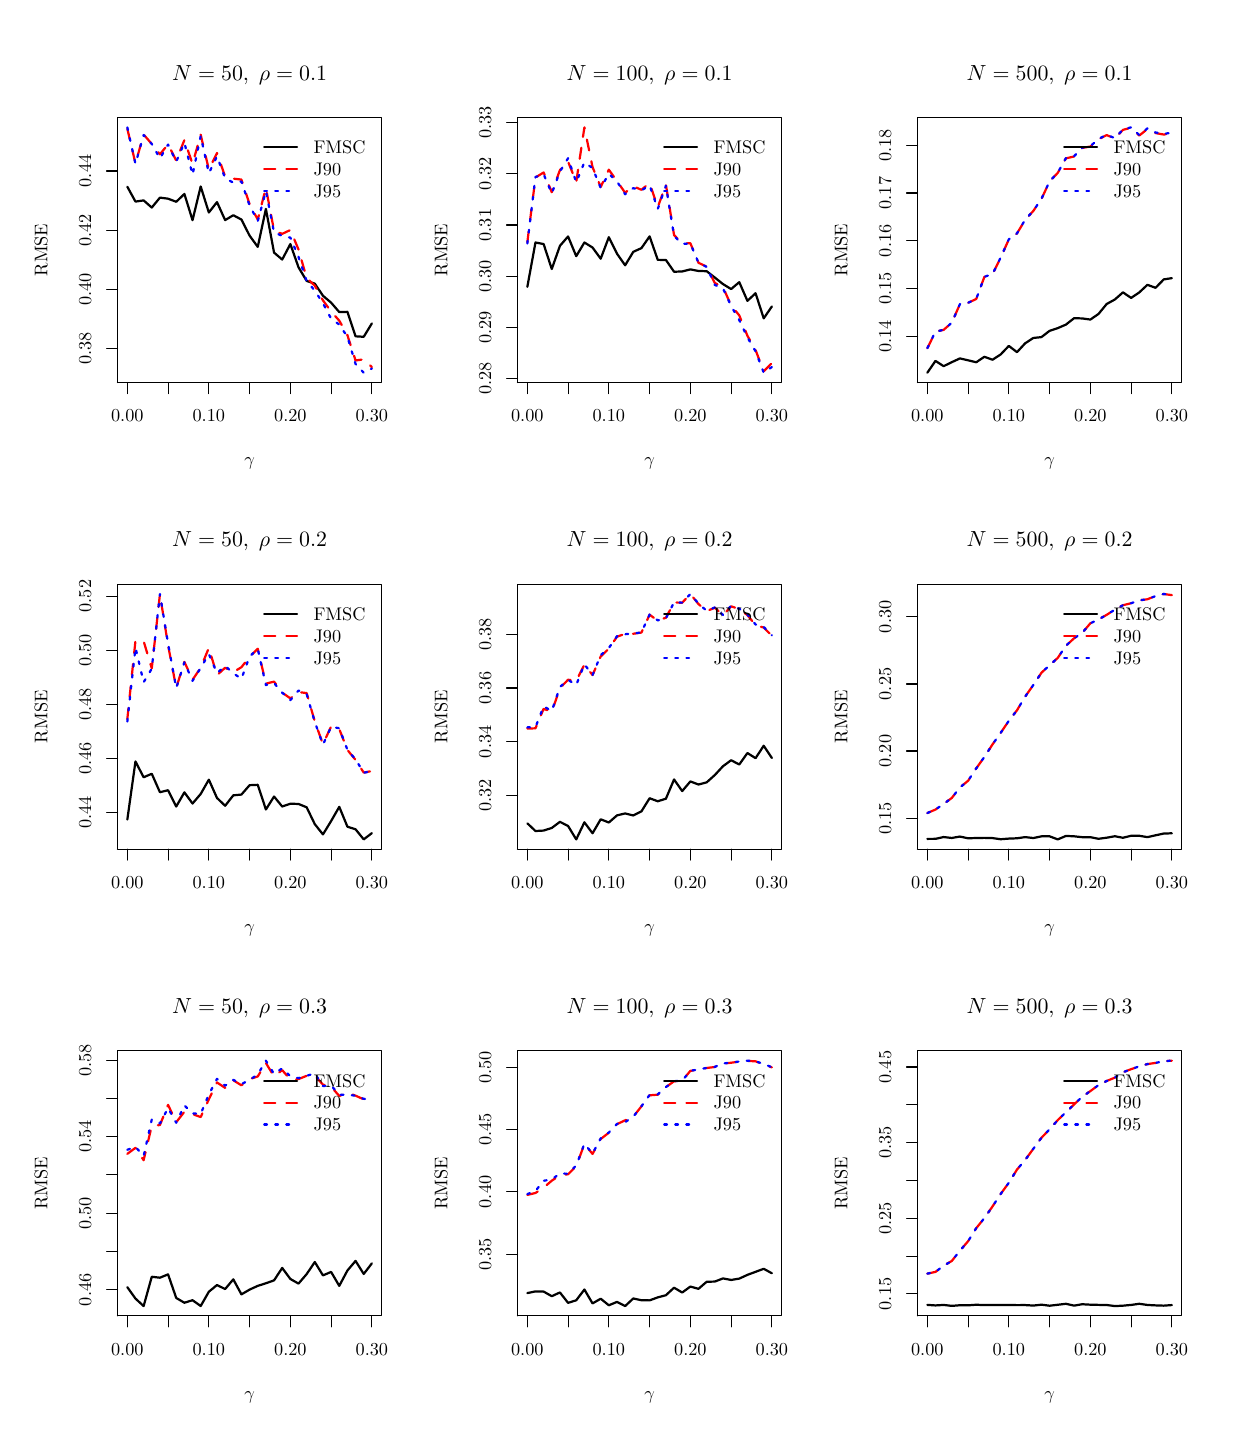
\begin{tikzpicture}[x=1pt,y=1pt]
\definecolor[named]{fillColor}{rgb}{1.00,1.00,1.00}
\path[use as bounding box,fill=fillColor,fill opacity=0.00] (0,0) rectangle (433.62,505.89);
\begin{scope}
\path[clip] ( 32.47,377.65) rectangle (127.91,473.42);
\definecolor[named]{drawColor}{rgb}{0.00,0.00,0.00}

\path[draw=drawColor,line width= 0.8pt,line join=round,line cap=round] ( 36.01,448.40) --
	( 38.95,443.04) --
	( 41.90,443.47) --
	( 44.84,440.88) --
	( 47.79,444.47) --
	( 50.73,444.09) --
	( 53.68,442.97) --
	( 56.63,445.80) --
	( 59.57,436.32) --
	( 62.52,448.50) --
	( 65.46,439.10) --
	( 68.41,442.85) --
	( 71.35,436.35) --
	( 74.30,438.11) --
	( 77.24,436.55) --
	( 80.19,430.73) --
	( 83.14,426.68) --
	( 86.08,440.41) --
	( 89.03,424.60) --
	( 91.97,422.10) --
	( 94.92,427.70) --
	( 97.86,419.31) --
	(100.81,414.37) --
	(103.75,413.40) --
	(106.70,409.01) --
	(109.65,406.52) --
	(112.59,403.11) --
	(115.54,403.20) --
	(118.48,394.36) --
	(121.43,394.18) --
	(124.37,399.02);
\end{scope}
\begin{scope}
\path[clip] (  0.00,  0.00) rectangle (433.62,505.89);
\definecolor[named]{drawColor}{rgb}{0.00,0.00,0.00}

\path[draw=drawColor,line width= 0.4pt,line join=round,line cap=round] ( 36.01,377.65) -- (124.37,377.65);

\path[draw=drawColor,line width= 0.4pt,line join=round,line cap=round] ( 36.01,377.65) -- ( 36.01,373.69);

\path[draw=drawColor,line width= 0.4pt,line join=round,line cap=round] ( 50.73,377.65) -- ( 50.73,373.69);

\path[draw=drawColor,line width= 0.4pt,line join=round,line cap=round] ( 65.46,377.65) -- ( 65.46,373.69);

\path[draw=drawColor,line width= 0.4pt,line join=round,line cap=round] ( 80.19,377.65) -- ( 80.19,373.69);

\path[draw=drawColor,line width= 0.4pt,line join=round,line cap=round] ( 94.92,377.65) -- ( 94.92,373.69);

\path[draw=drawColor,line width= 0.4pt,line join=round,line cap=round] (109.65,377.65) -- (109.65,373.69);

\path[draw=drawColor,line width= 0.4pt,line join=round,line cap=round] (124.37,377.65) -- (124.37,373.69);

\node[text=drawColor,anchor=base,inner sep=0pt, outer sep=0pt, scale=  0.66] at ( 36.01,363.40) {0.00};

\node[text=drawColor,anchor=base,inner sep=0pt, outer sep=0pt, scale=  0.66] at ( 65.46,363.40) {0.10};

\node[text=drawColor,anchor=base,inner sep=0pt, outer sep=0pt, scale=  0.66] at ( 94.92,363.40) {0.20};

\node[text=drawColor,anchor=base,inner sep=0pt, outer sep=0pt, scale=  0.66] at (124.37,363.40) {0.30};

\path[draw=drawColor,line width= 0.4pt,line join=round,line cap=round] ( 32.47,389.93) -- ( 32.47,454.11);

\path[draw=drawColor,line width= 0.4pt,line join=round,line cap=round] ( 32.47,389.93) -- ( 28.51,389.93);

\path[draw=drawColor,line width= 0.4pt,line join=round,line cap=round] ( 32.47,411.32) -- ( 28.51,411.32);

\path[draw=drawColor,line width= 0.4pt,line join=round,line cap=round] ( 32.47,432.72) -- ( 28.51,432.72);

\path[draw=drawColor,line width= 0.4pt,line join=round,line cap=round] ( 32.47,454.11) -- ( 28.51,454.11);

\node[text=drawColor,rotate= 90.00,anchor=base,inner sep=0pt, outer sep=0pt, scale=  0.66] at ( 22.97,389.93) {0.38};

\node[text=drawColor,rotate= 90.00,anchor=base,inner sep=0pt, outer sep=0pt, scale=  0.66] at ( 22.97,411.32) {0.40};

\node[text=drawColor,rotate= 90.00,anchor=base,inner sep=0pt, outer sep=0pt, scale=  0.66] at ( 22.97,432.72) {0.42};

\node[text=drawColor,rotate= 90.00,anchor=base,inner sep=0pt, outer sep=0pt, scale=  0.66] at ( 22.97,454.11) {0.44};

\path[draw=drawColor,line width= 0.4pt,line join=round,line cap=round] ( 32.47,377.65) --
	(127.91,377.65) --
	(127.91,473.42) --
	( 32.47,473.42) --
	( 32.47,377.65);
\end{scope}
\begin{scope}
\path[clip] (  0.00,337.26) rectangle (144.54,505.89);
\definecolor[named]{drawColor}{rgb}{0.00,0.00,0.00}

\node[text=drawColor,anchor=base,inner sep=0pt, outer sep=0pt, scale=  0.79] at ( 80.19,486.92) {\bfseries $N=50, \;\rho=0.1$};

\node[text=drawColor,anchor=base,inner sep=0pt, outer sep=0pt, scale=  0.66] at ( 80.19,347.56) {$\gamma$};

\node[text=drawColor,rotate= 90.00,anchor=base,inner sep=0pt, outer sep=0pt, scale=  0.66] at (  7.13,425.53) {RMSE};
\end{scope}
\begin{scope}
\path[clip] ( 32.47,377.65) rectangle (127.91,473.42);
\definecolor[named]{drawColor}{rgb}{1.00,0.00,0.00}

\path[draw=drawColor,line width= 0.8pt,dash pattern=on 4pt off 4pt ,line join=round,line cap=round] ( 36.01,469.35) --
	( 38.95,456.83) --
	( 41.90,467.26) --
	( 44.84,463.89) --
	( 47.79,460.13) --
	( 50.73,463.73) --
	( 53.68,457.89) --
	( 56.63,465.27) --
	( 59.57,456.67) --
	( 62.52,467.21) --
	( 65.46,454.64) --
	( 68.41,460.59) --
	( 71.35,452.09) --
	( 74.30,451.33) --
	( 77.24,450.99) --
	( 80.19,442.11) --
	( 83.14,436.54) --
	( 86.08,447.99) --
	( 89.03,432.52) --
	( 91.97,431.38) --
	( 94.92,432.77) --
	( 97.86,425.75) --
	(100.81,415.41) --
	(103.75,412.67) --
	(106.70,407.35) --
	(109.65,403.30) --
	(112.59,400.03) --
	(115.54,394.76) --
	(118.48,385.62) --
	(121.43,386.05) --
	(124.37,383.24);
\definecolor[named]{drawColor}{rgb}{0.00,0.00,1.00}

\path[draw=drawColor,line width= 0.8pt,dash pattern=on 1pt off 3pt ,line join=round,line cap=round] ( 36.01,469.87) --
	( 38.95,456.69) --
	( 41.90,467.11) --
	( 44.84,463.88) --
	( 47.79,458.63) --
	( 50.73,463.64) --
	( 53.68,457.45) --
	( 56.63,464.32) --
	( 59.57,452.73) --
	( 62.52,466.71) --
	( 65.46,453.28) --
	( 68.41,459.37) --
	( 71.35,451.48) --
	( 74.30,449.88) --
	( 77.24,450.29) --
	( 80.19,441.60) --
	( 83.14,435.99) --
	( 86.08,446.82) --
	( 89.03,431.92) --
	( 91.97,430.65) --
	( 94.92,430.02) --
	( 97.86,423.10) --
	(100.81,414.32) --
	(103.75,410.89) --
	(106.70,406.27) --
	(109.65,400.76) --
	(112.59,398.60) --
	(115.54,394.17) --
	(118.48,384.36) --
	(121.43,381.20) --
	(124.37,382.71);
\definecolor[named]{drawColor}{rgb}{0.00,0.00,0.00}

\path[draw=drawColor,line width= 0.8pt,line join=round,line cap=round] ( 85.47,462.63) -- ( 97.35,462.63);
\definecolor[named]{drawColor}{rgb}{1.00,0.00,0.00}

\path[draw=drawColor,line width= 0.8pt,dash pattern=on 4pt off 4pt ,line join=round,line cap=round] ( 85.47,454.71) -- ( 97.35,454.71);
\definecolor[named]{drawColor}{rgb}{0.00,0.00,1.00}

\path[draw=drawColor,line width= 0.8pt,dash pattern=on 1pt off 3pt ,line join=round,line cap=round] ( 85.47,446.79) -- ( 97.35,446.79);
\definecolor[named]{drawColor}{rgb}{0.00,0.00,0.00}

\node[text=drawColor,anchor=base west,inner sep=0pt, outer sep=0pt, scale=  0.66] at (103.29,460.35) {FMSC};

\node[text=drawColor,anchor=base west,inner sep=0pt, outer sep=0pt, scale=  0.66] at (103.29,452.43) {J90};

\node[text=drawColor,anchor=base west,inner sep=0pt, outer sep=0pt, scale=  0.66] at (103.29,444.51) {J95};
\end{scope}
\begin{scope}
\path[clip] (177.01,377.65) rectangle (272.45,473.42);
\definecolor[named]{drawColor}{rgb}{0.00,0.00,0.00}

\path[draw=drawColor,line width= 0.8pt,line join=round,line cap=round] (180.55,412.23) --
	(183.49,428.26) --
	(186.44,427.69) --
	(189.38,418.68) --
	(192.33,427.06) --
	(195.27,430.44) --
	(198.22,423.31) --
	(201.17,428.26) --
	(204.11,426.44) --
	(207.06,422.40) --
	(210.00,430.17) --
	(212.95,424.21) --
	(215.89,420.02) --
	(218.84,424.89) --
	(221.78,426.22) --
	(224.73,430.47) --
	(227.68,421.98) --
	(230.62,421.95) --
	(233.57,417.69) --
	(236.51,417.79) --
	(239.46,418.54) --
	(242.40,417.97) --
	(245.35,417.88) --
	(248.29,415.59) --
	(251.24,413.24) --
	(254.19,411.43) --
	(257.13,413.93) --
	(260.08,407.17) --
	(263.02,409.93) --
	(265.97,400.84) --
	(268.91,405.14);
\end{scope}
\begin{scope}
\path[clip] (  0.00,  0.00) rectangle (433.62,505.89);
\definecolor[named]{drawColor}{rgb}{0.00,0.00,0.00}

\path[draw=drawColor,line width= 0.4pt,line join=round,line cap=round] (180.55,377.65) -- (268.91,377.65);

\path[draw=drawColor,line width= 0.4pt,line join=round,line cap=round] (180.55,377.65) -- (180.55,373.69);

\path[draw=drawColor,line width= 0.4pt,line join=round,line cap=round] (195.27,377.65) -- (195.27,373.69);

\path[draw=drawColor,line width= 0.4pt,line join=round,line cap=round] (210.00,377.65) -- (210.00,373.69);

\path[draw=drawColor,line width= 0.4pt,line join=round,line cap=round] (224.73,377.65) -- (224.73,373.69);

\path[draw=drawColor,line width= 0.4pt,line join=round,line cap=round] (239.46,377.65) -- (239.46,373.69);

\path[draw=drawColor,line width= 0.4pt,line join=round,line cap=round] (254.19,377.65) -- (254.19,373.69);

\path[draw=drawColor,line width= 0.4pt,line join=round,line cap=round] (268.91,377.65) -- (268.91,373.69);

\node[text=drawColor,anchor=base,inner sep=0pt, outer sep=0pt, scale=  0.66] at (180.55,363.40) {0.00};

\node[text=drawColor,anchor=base,inner sep=0pt, outer sep=0pt, scale=  0.66] at (210.00,363.40) {0.10};

\node[text=drawColor,anchor=base,inner sep=0pt, outer sep=0pt, scale=  0.66] at (239.46,363.40) {0.20};

\node[text=drawColor,anchor=base,inner sep=0pt, outer sep=0pt, scale=  0.66] at (268.91,363.40) {0.30};

\path[draw=drawColor,line width= 0.4pt,line join=round,line cap=round] (177.01,379.18) -- (177.01,471.53);

\path[draw=drawColor,line width= 0.4pt,line join=round,line cap=round] (177.01,379.18) -- (173.05,379.18);

\path[draw=drawColor,line width= 0.4pt,line join=round,line cap=round] (177.01,397.65) -- (173.05,397.65);

\path[draw=drawColor,line width= 0.4pt,line join=round,line cap=round] (177.01,416.12) -- (173.05,416.12);

\path[draw=drawColor,line width= 0.4pt,line join=round,line cap=round] (177.01,434.59) -- (173.05,434.59);

\path[draw=drawColor,line width= 0.4pt,line join=round,line cap=round] (177.01,453.06) -- (173.05,453.06);

\path[draw=drawColor,line width= 0.4pt,line join=round,line cap=round] (177.01,471.53) -- (173.05,471.53);

\node[text=drawColor,rotate= 90.00,anchor=base,inner sep=0pt, outer sep=0pt, scale=  0.66] at (167.51,379.18) {0.28};

\node[text=drawColor,rotate= 90.00,anchor=base,inner sep=0pt, outer sep=0pt, scale=  0.66] at (167.51,397.65) {0.29};

\node[text=drawColor,rotate= 90.00,anchor=base,inner sep=0pt, outer sep=0pt, scale=  0.66] at (167.51,416.12) {0.30};

\node[text=drawColor,rotate= 90.00,anchor=base,inner sep=0pt, outer sep=0pt, scale=  0.66] at (167.51,434.59) {0.31};

\node[text=drawColor,rotate= 90.00,anchor=base,inner sep=0pt, outer sep=0pt, scale=  0.66] at (167.51,453.06) {0.32};

\node[text=drawColor,rotate= 90.00,anchor=base,inner sep=0pt, outer sep=0pt, scale=  0.66] at (167.51,471.53) {0.33};

\path[draw=drawColor,line width= 0.4pt,line join=round,line cap=round] (177.01,377.65) --
	(272.45,377.65) --
	(272.45,473.42) --
	(177.01,473.42) --
	(177.01,377.65);
\end{scope}
\begin{scope}
\path[clip] (144.54,337.26) rectangle (289.08,505.89);
\definecolor[named]{drawColor}{rgb}{0.00,0.00,0.00}

\node[text=drawColor,anchor=base,inner sep=0pt, outer sep=0pt, scale=  0.79] at (224.73,486.92) {\bfseries $N=100, \;\rho=0.1$};

\node[text=drawColor,anchor=base,inner sep=0pt, outer sep=0pt, scale=  0.66] at (224.73,347.56) {$\gamma$};

\node[text=drawColor,rotate= 90.00,anchor=base,inner sep=0pt, outer sep=0pt, scale=  0.66] at (151.67,425.54) {RMSE};
\end{scope}
\begin{scope}
\path[clip] (177.01,377.65) rectangle (272.45,473.42);
\definecolor[named]{drawColor}{rgb}{1.00,0.00,0.00}

\path[draw=drawColor,line width= 0.8pt,dash pattern=on 4pt off 4pt ,line join=round,line cap=round] (180.55,428.35) --
	(183.49,451.74) --
	(186.44,453.56) --
	(189.38,446.43) --
	(192.33,454.42) --
	(195.27,457.48) --
	(198.22,450.08) --
	(201.17,469.87) --
	(204.11,455.52) --
	(207.06,448.32) --
	(210.00,454.57) --
	(212.95,450.43) --
	(215.89,446.24) --
	(218.84,448.57) --
	(221.78,447.30) --
	(224.73,449.76) --
	(227.68,441.01) --
	(230.62,449.17) --
	(233.57,430.96) --
	(236.51,427.87) --
	(239.46,427.99) --
	(242.40,420.92) --
	(245.35,419.53) --
	(248.29,413.62) --
	(251.24,412.15) --
	(254.19,405.51) --
	(257.13,401.92) --
	(260.08,394.55) --
	(263.02,389.40) --
	(265.97,381.71) --
	(268.91,384.71);
\definecolor[named]{drawColor}{rgb}{0.00,0.00,1.00}

\path[draw=drawColor,line width= 0.8pt,dash pattern=on 1pt off 3pt ,line join=round,line cap=round] (180.55,427.89) --
	(183.49,451.92) --
	(186.44,452.94) --
	(189.38,445.98) --
	(192.33,453.89) --
	(195.27,458.70) --
	(198.22,450.03) --
	(201.17,457.22) --
	(204.11,455.16) --
	(207.06,447.99) --
	(210.00,453.08) --
	(212.95,450.33) --
	(215.89,445.69) --
	(218.84,447.90) --
	(221.78,447.08) --
	(224.73,448.92) --
	(227.68,440.40) --
	(230.62,448.79) --
	(233.57,430.58) --
	(236.51,427.77) --
	(239.46,427.88) --
	(242.40,420.96) --
	(245.35,419.44) --
	(248.29,412.93) --
	(251.24,411.68) --
	(254.19,405.31) --
	(257.13,400.20) --
	(260.08,393.94) --
	(263.02,388.96) --
	(265.97,381.20) --
	(268.91,383.25);
\definecolor[named]{drawColor}{rgb}{0.00,0.00,0.00}

\path[draw=drawColor,line width= 0.8pt,line join=round,line cap=round] (230.01,462.63) -- (241.89,462.63);
\definecolor[named]{drawColor}{rgb}{1.00,0.00,0.00}

\path[draw=drawColor,line width= 0.8pt,dash pattern=on 4pt off 4pt ,line join=round,line cap=round] (230.01,454.71) -- (241.89,454.71);
\definecolor[named]{drawColor}{rgb}{0.00,0.00,1.00}

\path[draw=drawColor,line width= 0.8pt,dash pattern=on 1pt off 3pt ,line join=round,line cap=round] (230.01,446.79) -- (241.89,446.79);
\definecolor[named]{drawColor}{rgb}{0.00,0.00,0.00}

\node[text=drawColor,anchor=base west,inner sep=0pt, outer sep=0pt, scale=  0.66] at (247.83,460.35) {FMSC};

\node[text=drawColor,anchor=base west,inner sep=0pt, outer sep=0pt, scale=  0.66] at (247.83,452.43) {J90};

\node[text=drawColor,anchor=base west,inner sep=0pt, outer sep=0pt, scale=  0.66] at (247.83,444.51) {J95};
\end{scope}
\begin{scope}
\path[clip] (321.55,377.65) rectangle (416.99,473.42);
\definecolor[named]{drawColor}{rgb}{0.00,0.00,0.00}

\path[draw=drawColor,line width= 0.8pt,line join=round,line cap=round] (325.09,381.20) --
	(328.03,385.47) --
	(330.98,383.57) --
	(333.92,385.01) --
	(336.87,386.37) --
	(339.81,385.69) --
	(342.76,384.98) --
	(345.71,386.96) --
	(348.65,385.89) --
	(351.60,387.82) --
	(354.54,390.89) --
	(357.49,388.63) --
	(360.43,391.83) --
	(363.38,393.76) --
	(366.32,394.07) --
	(369.27,396.35) --
	(372.22,397.32) --
	(375.16,398.59) --
	(378.11,400.90) --
	(381.05,400.82) --
	(384.00,400.41) --
	(386.94,402.44) --
	(389.89,406.03) --
	(392.83,407.65) --
	(395.78,410.24) --
	(398.73,408.23) --
	(401.67,410.22) --
	(404.62,412.97) --
	(407.56,411.88) --
	(410.51,414.92) --
	(413.45,415.38);
\end{scope}
\begin{scope}
\path[clip] (  0.00,  0.00) rectangle (433.62,505.89);
\definecolor[named]{drawColor}{rgb}{0.00,0.00,0.00}

\path[draw=drawColor,line width= 0.4pt,line join=round,line cap=round] (325.09,377.65) -- (413.45,377.65);

\path[draw=drawColor,line width= 0.4pt,line join=round,line cap=round] (325.09,377.65) -- (325.09,373.69);

\path[draw=drawColor,line width= 0.4pt,line join=round,line cap=round] (339.81,377.65) -- (339.81,373.69);

\path[draw=drawColor,line width= 0.4pt,line join=round,line cap=round] (354.54,377.65) -- (354.54,373.69);

\path[draw=drawColor,line width= 0.4pt,line join=round,line cap=round] (369.27,377.65) -- (369.27,373.69);

\path[draw=drawColor,line width= 0.4pt,line join=round,line cap=round] (384.00,377.65) -- (384.00,373.69);

\path[draw=drawColor,line width= 0.4pt,line join=round,line cap=round] (398.73,377.65) -- (398.73,373.69);

\path[draw=drawColor,line width= 0.4pt,line join=round,line cap=round] (413.45,377.65) -- (413.45,373.69);

\node[text=drawColor,anchor=base,inner sep=0pt, outer sep=0pt, scale=  0.66] at (325.09,363.40) {0.00};

\node[text=drawColor,anchor=base,inner sep=0pt, outer sep=0pt, scale=  0.66] at (354.54,363.40) {0.10};

\node[text=drawColor,anchor=base,inner sep=0pt, outer sep=0pt, scale=  0.66] at (384.00,363.40) {0.20};

\node[text=drawColor,anchor=base,inner sep=0pt, outer sep=0pt, scale=  0.66] at (413.45,363.40) {0.30};

\path[draw=drawColor,line width= 0.4pt,line join=round,line cap=round] (321.55,394.27) -- (321.55,463.45);

\path[draw=drawColor,line width= 0.4pt,line join=round,line cap=round] (321.55,394.27) -- (317.59,394.27);

\path[draw=drawColor,line width= 0.4pt,line join=round,line cap=round] (321.55,411.56) -- (317.59,411.56);

\path[draw=drawColor,line width= 0.4pt,line join=round,line cap=round] (321.55,428.86) -- (317.59,428.86);

\path[draw=drawColor,line width= 0.4pt,line join=round,line cap=round] (321.55,446.15) -- (317.59,446.15);

\path[draw=drawColor,line width= 0.4pt,line join=round,line cap=round] (321.55,463.45) -- (317.59,463.45);

\node[text=drawColor,rotate= 90.00,anchor=base,inner sep=0pt, outer sep=0pt, scale=  0.66] at (312.05,394.27) {0.14};

\node[text=drawColor,rotate= 90.00,anchor=base,inner sep=0pt, outer sep=0pt, scale=  0.66] at (312.05,411.56) {0.15};

\node[text=drawColor,rotate= 90.00,anchor=base,inner sep=0pt, outer sep=0pt, scale=  0.66] at (312.05,428.86) {0.16};

\node[text=drawColor,rotate= 90.00,anchor=base,inner sep=0pt, outer sep=0pt, scale=  0.66] at (312.05,446.15) {0.17};

\node[text=drawColor,rotate= 90.00,anchor=base,inner sep=0pt, outer sep=0pt, scale=  0.66] at (312.05,463.45) {0.18};

\path[draw=drawColor,line width= 0.4pt,line join=round,line cap=round] (321.55,377.65) --
	(416.99,377.65) --
	(416.99,473.42) --
	(321.55,473.42) --
	(321.55,377.65);
\end{scope}
\begin{scope}
\path[clip] (289.08,337.26) rectangle (433.62,505.89);
\definecolor[named]{drawColor}{rgb}{0.00,0.00,0.00}

\node[text=drawColor,anchor=base,inner sep=0pt, outer sep=0pt, scale=  0.79] at (369.27,486.92) {\bfseries $N=500, \;\rho=0.1$};

\node[text=drawColor,anchor=base,inner sep=0pt, outer sep=0pt, scale=  0.66] at (369.27,347.56) {$\gamma$};

\node[text=drawColor,rotate= 90.00,anchor=base,inner sep=0pt, outer sep=0pt, scale=  0.66] at (296.21,425.53) {RMSE};
\end{scope}
\begin{scope}
\path[clip] (321.55,377.65) rectangle (416.99,473.42);
\definecolor[named]{drawColor}{rgb}{1.00,0.00,0.00}

\path[draw=drawColor,line width= 0.8pt,dash pattern=on 4pt off 4pt ,line join=round,line cap=round] (325.09,390.05) --
	(328.03,396.03) --
	(330.98,396.69) --
	(333.92,399.26) --
	(336.87,405.99) --
	(339.81,406.46) --
	(342.76,407.84) --
	(345.71,415.86) --
	(348.65,416.85) --
	(351.60,422.79) --
	(354.54,429.40) --
	(357.49,431.54) --
	(360.43,436.43) --
	(363.38,439.66) --
	(366.32,444.00) --
	(369.27,450.32) --
	(372.22,453.42) --
	(375.16,458.66) --
	(378.11,459.33) --
	(381.05,462.43) --
	(384.00,462.93) --
	(386.94,465.52) --
	(389.89,467.08) --
	(392.83,465.81) --
	(395.78,468.96) --
	(398.73,469.73) --
	(401.67,466.91) --
	(404.62,469.27) --
	(407.56,467.79) --
	(410.51,467.27) --
	(413.45,467.70);
\definecolor[named]{drawColor}{rgb}{0.00,0.00,1.00}

\path[draw=drawColor,line width= 0.8pt,dash pattern=on 1pt off 3pt ,line join=round,line cap=round] (325.09,390.09) --
	(328.03,396.04) --
	(330.98,396.71) --
	(333.92,399.27) --
	(336.87,406.00) --
	(339.81,406.47) --
	(342.76,407.85) --
	(345.71,415.86) --
	(348.65,416.88) --
	(351.60,422.82) --
	(354.54,429.42) --
	(357.49,431.57) --
	(360.43,436.47) --
	(363.38,439.70) --
	(366.32,444.02) --
	(369.27,450.38) --
	(372.22,453.48) --
	(375.16,458.73) --
	(378.11,459.43) --
	(381.05,462.53) --
	(384.00,463.06) --
	(386.94,465.67) --
	(389.89,467.21) --
	(392.83,465.94) --
	(395.78,469.10) --
	(398.73,469.87) --
	(401.67,467.06) --
	(404.62,469.50) --
	(407.56,468.01) --
	(410.51,467.52) --
	(413.45,467.92);
\definecolor[named]{drawColor}{rgb}{0.00,0.00,0.00}

\path[draw=drawColor,line width= 0.8pt,line join=round,line cap=round] (374.55,462.63) -- (386.43,462.63);
\definecolor[named]{drawColor}{rgb}{1.00,0.00,0.00}

\path[draw=drawColor,line width= 0.8pt,dash pattern=on 4pt off 4pt ,line join=round,line cap=round] (374.55,454.71) -- (386.43,454.71);
\definecolor[named]{drawColor}{rgb}{0.00,0.00,1.00}

\path[draw=drawColor,line width= 0.8pt,dash pattern=on 1pt off 3pt ,line join=round,line cap=round] (374.55,446.79) -- (386.43,446.79);
\definecolor[named]{drawColor}{rgb}{0.00,0.00,0.00}

\node[text=drawColor,anchor=base west,inner sep=0pt, outer sep=0pt, scale=  0.66] at (392.37,460.35) {FMSC};

\node[text=drawColor,anchor=base west,inner sep=0pt, outer sep=0pt, scale=  0.66] at (392.37,452.43) {J90};

\node[text=drawColor,anchor=base west,inner sep=0pt, outer sep=0pt, scale=  0.66] at (392.37,444.51) {J95};
\end{scope}
\begin{scope}
\path[clip] ( 32.47,209.02) rectangle (127.91,304.79);
\definecolor[named]{drawColor}{rgb}{0.00,0.00,0.00}

\path[draw=drawColor,line width= 0.8pt,line join=round,line cap=round] ( 36.01,219.74) --
	( 38.95,240.74) --
	( 41.90,235.02) --
	( 44.84,236.28) --
	( 47.79,229.62) --
	( 50.73,230.33) --
	( 53.68,224.45) --
	( 56.63,229.57) --
	( 59.57,225.53) --
	( 62.52,228.99) --
	( 65.46,234.16) --
	( 68.41,227.54) --
	( 71.35,224.72) --
	( 74.30,228.49) --
	( 77.24,228.77) --
	( 80.19,232.16) --
	( 83.14,232.29) --
	( 86.08,223.38) --
	( 89.03,228.06) --
	( 91.97,224.45) --
	( 94.92,225.46) --
	( 97.86,225.38) --
	(100.81,224.17) --
	(103.75,218.08) --
	(106.70,214.38) --
	(109.65,219.20) --
	(112.59,224.33) --
	(115.54,217.16) --
	(118.48,216.22) --
	(121.43,212.57) --
	(124.37,214.84);
\end{scope}
\begin{scope}
\path[clip] (  0.00,  0.00) rectangle (433.62,505.89);
\definecolor[named]{drawColor}{rgb}{0.00,0.00,0.00}

\path[draw=drawColor,line width= 0.4pt,line join=round,line cap=round] ( 36.01,209.02) -- (124.37,209.02);

\path[draw=drawColor,line width= 0.4pt,line join=round,line cap=round] ( 36.01,209.02) -- ( 36.01,205.06);

\path[draw=drawColor,line width= 0.4pt,line join=round,line cap=round] ( 50.73,209.02) -- ( 50.73,205.06);

\path[draw=drawColor,line width= 0.4pt,line join=round,line cap=round] ( 65.46,209.02) -- ( 65.46,205.06);

\path[draw=drawColor,line width= 0.4pt,line join=round,line cap=round] ( 80.19,209.02) -- ( 80.19,205.06);

\path[draw=drawColor,line width= 0.4pt,line join=round,line cap=round] ( 94.92,209.02) -- ( 94.92,205.06);

\path[draw=drawColor,line width= 0.4pt,line join=round,line cap=round] (109.65,209.02) -- (109.65,205.06);

\path[draw=drawColor,line width= 0.4pt,line join=round,line cap=round] (124.37,209.02) -- (124.37,205.06);

\node[text=drawColor,anchor=base,inner sep=0pt, outer sep=0pt, scale=  0.66] at ( 36.01,194.77) {0.00};

\node[text=drawColor,anchor=base,inner sep=0pt, outer sep=0pt, scale=  0.66] at ( 65.46,194.77) {0.10};

\node[text=drawColor,anchor=base,inner sep=0pt, outer sep=0pt, scale=  0.66] at ( 94.92,194.77) {0.20};

\node[text=drawColor,anchor=base,inner sep=0pt, outer sep=0pt, scale=  0.66] at (124.37,194.77) {0.30};

\path[draw=drawColor,line width= 0.4pt,line join=round,line cap=round] ( 32.47,222.38) -- ( 32.47,300.49);

\path[draw=drawColor,line width= 0.4pt,line join=round,line cap=round] ( 32.47,222.38) -- ( 28.51,222.38);

\path[draw=drawColor,line width= 0.4pt,line join=round,line cap=round] ( 32.47,241.91) -- ( 28.51,241.91);

\path[draw=drawColor,line width= 0.4pt,line join=round,line cap=round] ( 32.47,261.44) -- ( 28.51,261.44);

\path[draw=drawColor,line width= 0.4pt,line join=round,line cap=round] ( 32.47,280.96) -- ( 28.51,280.96);

\path[draw=drawColor,line width= 0.4pt,line join=round,line cap=round] ( 32.47,300.49) -- ( 28.51,300.49);

\node[text=drawColor,rotate= 90.00,anchor=base,inner sep=0pt, outer sep=0pt, scale=  0.66] at ( 22.97,222.38) {0.44};

\node[text=drawColor,rotate= 90.00,anchor=base,inner sep=0pt, outer sep=0pt, scale=  0.66] at ( 22.97,241.91) {0.46};

\node[text=drawColor,rotate= 90.00,anchor=base,inner sep=0pt, outer sep=0pt, scale=  0.66] at ( 22.97,261.44) {0.48};

\node[text=drawColor,rotate= 90.00,anchor=base,inner sep=0pt, outer sep=0pt, scale=  0.66] at ( 22.97,280.96) {0.50};

\node[text=drawColor,rotate= 90.00,anchor=base,inner sep=0pt, outer sep=0pt, scale=  0.66] at ( 22.97,300.49) {0.52};

\path[draw=drawColor,line width= 0.4pt,line join=round,line cap=round] ( 32.47,209.02) --
	(127.91,209.02) --
	(127.91,304.79) --
	( 32.47,304.79) --
	( 32.47,209.02);
\end{scope}
\begin{scope}
\path[clip] (  0.00,168.63) rectangle (144.54,337.26);
\definecolor[named]{drawColor}{rgb}{0.00,0.00,0.00}

\node[text=drawColor,anchor=base,inner sep=0pt, outer sep=0pt, scale=  0.79] at ( 80.19,318.29) {\bfseries $N=50, \;\rho=0.2$};

\node[text=drawColor,anchor=base,inner sep=0pt, outer sep=0pt, scale=  0.66] at ( 80.19,178.93) {$\gamma$};

\node[text=drawColor,rotate= 90.00,anchor=base,inner sep=0pt, outer sep=0pt, scale=  0.66] at (  7.13,256.90) {RMSE};
\end{scope}
\begin{scope}
\path[clip] ( 32.47,209.02) rectangle (127.91,304.79);
\definecolor[named]{drawColor}{rgb}{1.00,0.00,0.00}

\path[draw=drawColor,line width= 0.8pt,dash pattern=on 4pt off 4pt ,line join=round,line cap=round] ( 36.01,256.06) --
	( 38.95,284.37) --
	( 41.90,284.21) --
	( 44.84,274.37) --
	( 47.79,301.13) --
	( 50.73,282.74) --
	( 53.68,267.35) --
	( 56.63,276.72) --
	( 59.57,270.25) --
	( 62.52,274.58) --
	( 65.46,281.77) --
	( 68.41,271.92) --
	( 71.35,274.60) --
	( 74.30,273.01) --
	( 77.24,274.80) --
	( 80.19,278.52) --
	( 83.14,281.45) --
	( 86.08,268.87) --
	( 89.03,269.57) --
	( 91.97,265.61) --
	( 94.92,263.53) --
	( 97.86,265.79) --
	(100.81,265.45) --
	(103.75,255.20) --
	(106.70,246.99) --
	(109.65,253.38) --
	(112.59,252.44) --
	(115.54,244.88) --
	(118.48,241.30) --
	(121.43,236.71) --
	(124.37,237.28);
\definecolor[named]{drawColor}{rgb}{0.00,0.00,1.00}

\path[draw=drawColor,line width= 0.8pt,dash pattern=on 1pt off 3pt ,line join=round,line cap=round] ( 36.01,255.15) --
	( 38.95,281.88) --
	( 41.90,269.36) --
	( 44.84,274.25) --
	( 47.79,301.24) --
	( 50.73,283.33) --
	( 53.68,267.24) --
	( 56.63,276.56) --
	( 59.57,269.86) --
	( 62.52,274.53) --
	( 65.46,279.56) --
	( 68.41,272.64) --
	( 71.35,275.25) --
	( 74.30,272.60) --
	( 77.24,270.61) --
	( 80.19,278.67) --
	( 83.14,281.40) --
	( 86.08,268.34) --
	( 89.03,269.07) --
	( 91.97,265.59) --
	( 94.92,262.90) --
	( 97.86,266.36) --
	(100.81,265.11) --
	(103.75,254.98) --
	(106.70,246.81) --
	(109.65,253.26) --
	(112.59,252.74) --
	(115.54,244.95) --
	(118.48,241.50) --
	(121.43,236.65) --
	(124.37,237.22);
\definecolor[named]{drawColor}{rgb}{0.00,0.00,0.00}

\path[draw=drawColor,line width= 0.8pt,line join=round,line cap=round] ( 85.47,294.00) -- ( 97.35,294.00);
\definecolor[named]{drawColor}{rgb}{1.00,0.00,0.00}

\path[draw=drawColor,line width= 0.8pt,dash pattern=on 4pt off 4pt ,line join=round,line cap=round] ( 85.47,286.08) -- ( 97.35,286.08);
\definecolor[named]{drawColor}{rgb}{0.00,0.00,1.00}

\path[draw=drawColor,line width= 0.8pt,dash pattern=on 1pt off 3pt ,line join=round,line cap=round] ( 85.47,278.16) -- ( 97.35,278.16);
\definecolor[named]{drawColor}{rgb}{0.00,0.00,0.00}

\node[text=drawColor,anchor=base west,inner sep=0pt, outer sep=0pt, scale=  0.66] at (103.29,291.72) {FMSC};

\node[text=drawColor,anchor=base west,inner sep=0pt, outer sep=0pt, scale=  0.66] at (103.29,283.80) {J90};

\node[text=drawColor,anchor=base west,inner sep=0pt, outer sep=0pt, scale=  0.66] at (103.29,275.88) {J95};
\end{scope}
\begin{scope}
\path[clip] (177.01,209.02) rectangle (272.45,304.79);
\definecolor[named]{drawColor}{rgb}{0.00,0.00,0.00}

\path[draw=drawColor,line width= 0.8pt,line join=round,line cap=round] (180.55,218.38) --
	(183.49,215.60) --
	(186.44,215.76) --
	(189.38,216.71) --
	(192.33,218.92) --
	(195.27,217.42) --
	(198.22,212.57) --
	(201.17,218.75) --
	(204.11,214.78) --
	(207.06,219.84) --
	(210.00,218.67) --
	(212.95,221.25) --
	(215.89,221.95) --
	(218.84,221.22) --
	(221.78,222.70) --
	(224.73,227.44) --
	(227.68,226.35) --
	(230.62,227.27) --
	(233.57,234.23) --
	(236.51,230.03) --
	(239.46,233.52) --
	(242.40,232.40) --
	(245.35,233.18) --
	(248.29,235.82) --
	(251.24,239.00) --
	(254.19,241.18) --
	(257.13,239.63) --
	(260.08,243.78) --
	(263.02,241.92) --
	(265.97,246.42) --
	(268.91,241.99);
\end{scope}
\begin{scope}
\path[clip] (  0.00,  0.00) rectangle (433.62,505.89);
\definecolor[named]{drawColor}{rgb}{0.00,0.00,0.00}

\path[draw=drawColor,line width= 0.4pt,line join=round,line cap=round] (180.55,209.02) -- (268.91,209.02);

\path[draw=drawColor,line width= 0.4pt,line join=round,line cap=round] (180.55,209.02) -- (180.55,205.06);

\path[draw=drawColor,line width= 0.4pt,line join=round,line cap=round] (195.27,209.02) -- (195.27,205.06);

\path[draw=drawColor,line width= 0.4pt,line join=round,line cap=round] (210.00,209.02) -- (210.00,205.06);

\path[draw=drawColor,line width= 0.4pt,line join=round,line cap=round] (224.73,209.02) -- (224.73,205.06);

\path[draw=drawColor,line width= 0.4pt,line join=round,line cap=round] (239.46,209.02) -- (239.46,205.06);

\path[draw=drawColor,line width= 0.4pt,line join=round,line cap=round] (254.19,209.02) -- (254.19,205.06);

\path[draw=drawColor,line width= 0.4pt,line join=round,line cap=round] (268.91,209.02) -- (268.91,205.06);

\node[text=drawColor,anchor=base,inner sep=0pt, outer sep=0pt, scale=  0.66] at (180.55,194.77) {0.00};

\node[text=drawColor,anchor=base,inner sep=0pt, outer sep=0pt, scale=  0.66] at (210.00,194.77) {0.10};

\node[text=drawColor,anchor=base,inner sep=0pt, outer sep=0pt, scale=  0.66] at (239.46,194.77) {0.20};

\node[text=drawColor,anchor=base,inner sep=0pt, outer sep=0pt, scale=  0.66] at (268.91,194.77) {0.30};

\path[draw=drawColor,line width= 0.4pt,line join=round,line cap=round] (177.01,228.35) -- (177.01,286.73);

\path[draw=drawColor,line width= 0.4pt,line join=round,line cap=round] (177.01,228.35) -- (173.05,228.35);

\path[draw=drawColor,line width= 0.4pt,line join=round,line cap=round] (177.01,247.81) -- (173.05,247.81);

\path[draw=drawColor,line width= 0.4pt,line join=round,line cap=round] (177.01,267.27) -- (173.05,267.27);

\path[draw=drawColor,line width= 0.4pt,line join=round,line cap=round] (177.01,286.73) -- (173.05,286.73);

\node[text=drawColor,rotate= 90.00,anchor=base,inner sep=0pt, outer sep=0pt, scale=  0.66] at (167.51,228.35) {0.32};

\node[text=drawColor,rotate= 90.00,anchor=base,inner sep=0pt, outer sep=0pt, scale=  0.66] at (167.51,247.81) {0.34};

\node[text=drawColor,rotate= 90.00,anchor=base,inner sep=0pt, outer sep=0pt, scale=  0.66] at (167.51,267.27) {0.36};

\node[text=drawColor,rotate= 90.00,anchor=base,inner sep=0pt, outer sep=0pt, scale=  0.66] at (167.51,286.73) {0.38};

\path[draw=drawColor,line width= 0.4pt,line join=round,line cap=round] (177.01,209.02) --
	(272.45,209.02) --
	(272.45,304.79) --
	(177.01,304.79) --
	(177.01,209.02);
\end{scope}
\begin{scope}
\path[clip] (144.54,168.63) rectangle (289.08,337.26);
\definecolor[named]{drawColor}{rgb}{0.00,0.00,0.00}

\node[text=drawColor,anchor=base,inner sep=0pt, outer sep=0pt, scale=  0.79] at (224.73,318.29) {\bfseries $N=100, \;\rho=0.2$};

\node[text=drawColor,anchor=base,inner sep=0pt, outer sep=0pt, scale=  0.66] at (224.73,178.93) {$\gamma$};

\node[text=drawColor,rotate= 90.00,anchor=base,inner sep=0pt, outer sep=0pt, scale=  0.66] at (151.67,256.90) {RMSE};
\end{scope}
\begin{scope}
\path[clip] (177.01,209.02) rectangle (272.45,304.79);
\definecolor[named]{drawColor}{rgb}{1.00,0.00,0.00}

\path[draw=drawColor,line width= 0.8pt,dash pattern=on 4pt off 4pt ,line join=round,line cap=round] (180.55,252.62) --
	(183.49,252.71) --
	(186.44,259.76) --
	(189.38,258.64) --
	(192.33,267.25) --
	(195.27,270.27) --
	(198.22,269.84) --
	(201.17,275.71) --
	(204.11,271.96) --
	(207.06,278.67) --
	(210.00,281.49) --
	(212.95,285.81) --
	(215.89,286.87) --
	(218.84,286.88) --
	(221.78,287.32) --
	(224.73,293.75) --
	(227.68,291.61) --
	(230.62,292.68) --
	(233.57,298.16) --
	(236.51,298.10) --
	(239.46,301.24) --
	(242.40,297.61) --
	(245.35,295.06) --
	(248.29,296.27) --
	(251.24,293.55) --
	(254.19,296.79) --
	(257.13,295.79) --
	(260.08,293.62) --
	(263.02,289.95) --
	(265.97,289.12) --
	(268.91,286.16);
\definecolor[named]{drawColor}{rgb}{0.00,0.00,1.00}

\path[draw=drawColor,line width= 0.8pt,dash pattern=on 1pt off 3pt ,line join=round,line cap=round] (180.55,253.07) --
	(183.49,253.12) --
	(186.44,260.66) --
	(189.38,258.95) --
	(192.33,267.67) --
	(195.27,270.20) --
	(198.22,268.37) --
	(201.17,275.86) --
	(204.11,271.93) --
	(207.06,279.14) --
	(210.00,281.72) --
	(212.95,286.00) --
	(215.89,286.72) --
	(218.84,286.96) --
	(221.78,287.37) --
	(224.73,293.83) --
	(227.68,291.72) --
	(230.62,292.42) --
	(233.57,298.23) --
	(236.51,298.12) --
	(239.46,301.23) --
	(242.40,297.77) --
	(245.35,295.17) --
	(248.29,296.39) --
	(251.24,293.69) --
	(254.19,297.00) --
	(257.13,295.92) --
	(260.08,293.84) --
	(263.02,290.23) --
	(265.97,289.31) --
	(268.91,286.34);
\definecolor[named]{drawColor}{rgb}{0.00,0.00,0.00}

\path[draw=drawColor,line width= 0.8pt,line join=round,line cap=round] (230.01,294.00) -- (241.89,294.00);
\definecolor[named]{drawColor}{rgb}{1.00,0.00,0.00}

\path[draw=drawColor,line width= 0.8pt,dash pattern=on 4pt off 4pt ,line join=round,line cap=round] (230.01,286.08) -- (241.89,286.08);
\definecolor[named]{drawColor}{rgb}{0.00,0.00,1.00}

\path[draw=drawColor,line width= 0.8pt,dash pattern=on 1pt off 3pt ,line join=round,line cap=round] (230.01,278.16) -- (241.89,278.16);
\definecolor[named]{drawColor}{rgb}{0.00,0.00,0.00}

\node[text=drawColor,anchor=base west,inner sep=0pt, outer sep=0pt, scale=  0.66] at (247.83,291.72) {FMSC};

\node[text=drawColor,anchor=base west,inner sep=0pt, outer sep=0pt, scale=  0.66] at (247.83,283.80) {J90};

\node[text=drawColor,anchor=base west,inner sep=0pt, outer sep=0pt, scale=  0.66] at (247.83,275.88) {J95};
\end{scope}
\begin{scope}
\path[clip] (321.55,209.02) rectangle (416.99,304.79);
\definecolor[named]{drawColor}{rgb}{0.00,0.00,0.00}

\path[draw=drawColor,line width= 0.8pt,line join=round,line cap=round] (325.09,212.75) --
	(328.03,212.77) --
	(330.98,213.42) --
	(333.92,213.09) --
	(336.87,213.59) --
	(339.81,212.97) --
	(342.76,213.07) --
	(345.71,213.12) --
	(348.65,213.04) --
	(351.60,212.63) --
	(354.54,212.86) --
	(357.49,212.97) --
	(360.43,213.40) --
	(363.38,213.06) --
	(366.32,213.67) --
	(369.27,213.68) --
	(372.22,212.57) --
	(375.16,213.82) --
	(378.11,213.69) --
	(381.05,213.37) --
	(384.00,213.38) --
	(386.94,212.79) --
	(389.89,213.18) --
	(392.83,213.71) --
	(395.78,213.16) --
	(398.73,213.89) --
	(401.67,213.88) --
	(404.62,213.39) --
	(407.56,214.05) --
	(410.51,214.68) --
	(413.45,214.78);
\end{scope}
\begin{scope}
\path[clip] (  0.00,  0.00) rectangle (433.62,505.89);
\definecolor[named]{drawColor}{rgb}{0.00,0.00,0.00}

\path[draw=drawColor,line width= 0.4pt,line join=round,line cap=round] (325.09,209.02) -- (413.45,209.02);

\path[draw=drawColor,line width= 0.4pt,line join=round,line cap=round] (325.09,209.02) -- (325.09,205.06);

\path[draw=drawColor,line width= 0.4pt,line join=round,line cap=round] (339.81,209.02) -- (339.81,205.06);

\path[draw=drawColor,line width= 0.4pt,line join=round,line cap=round] (354.54,209.02) -- (354.54,205.06);

\path[draw=drawColor,line width= 0.4pt,line join=round,line cap=round] (369.27,209.02) -- (369.27,205.06);

\path[draw=drawColor,line width= 0.4pt,line join=round,line cap=round] (384.00,209.02) -- (384.00,205.06);

\path[draw=drawColor,line width= 0.4pt,line join=round,line cap=round] (398.73,209.02) -- (398.73,205.06);

\path[draw=drawColor,line width= 0.4pt,line join=round,line cap=round] (413.45,209.02) -- (413.45,205.06);

\node[text=drawColor,anchor=base,inner sep=0pt, outer sep=0pt, scale=  0.66] at (325.09,194.77) {0.00};

\node[text=drawColor,anchor=base,inner sep=0pt, outer sep=0pt, scale=  0.66] at (354.54,194.77) {0.10};

\node[text=drawColor,anchor=base,inner sep=0pt, outer sep=0pt, scale=  0.66] at (384.00,194.77) {0.20};

\node[text=drawColor,anchor=base,inner sep=0pt, outer sep=0pt, scale=  0.66] at (413.45,194.77) {0.30};

\path[draw=drawColor,line width= 0.4pt,line join=round,line cap=round] (321.55,220.25) -- (321.55,292.99);

\path[draw=drawColor,line width= 0.4pt,line join=round,line cap=round] (321.55,220.25) -- (317.59,220.25);

\path[draw=drawColor,line width= 0.4pt,line join=round,line cap=round] (321.55,244.50) -- (317.59,244.50);

\path[draw=drawColor,line width= 0.4pt,line join=round,line cap=round] (321.55,268.74) -- (317.59,268.74);

\path[draw=drawColor,line width= 0.4pt,line join=round,line cap=round] (321.55,292.99) -- (317.59,292.99);

\node[text=drawColor,rotate= 90.00,anchor=base,inner sep=0pt, outer sep=0pt, scale=  0.66] at (312.05,220.25) {0.15};

\node[text=drawColor,rotate= 90.00,anchor=base,inner sep=0pt, outer sep=0pt, scale=  0.66] at (312.05,244.50) {0.20};

\node[text=drawColor,rotate= 90.00,anchor=base,inner sep=0pt, outer sep=0pt, scale=  0.66] at (312.05,268.74) {0.25};

\node[text=drawColor,rotate= 90.00,anchor=base,inner sep=0pt, outer sep=0pt, scale=  0.66] at (312.05,292.99) {0.30};

\path[draw=drawColor,line width= 0.4pt,line join=round,line cap=round] (321.55,209.02) --
	(416.99,209.02) --
	(416.99,304.79) --
	(321.55,304.79) --
	(321.55,209.02);
\end{scope}
\begin{scope}
\path[clip] (289.08,168.63) rectangle (433.62,337.26);
\definecolor[named]{drawColor}{rgb}{0.00,0.00,0.00}

\node[text=drawColor,anchor=base,inner sep=0pt, outer sep=0pt, scale=  0.79] at (369.27,318.29) {\bfseries $N=500, \;\rho=0.2$};

\node[text=drawColor,anchor=base,inner sep=0pt, outer sep=0pt, scale=  0.66] at (369.27,178.93) {$\gamma$};

\node[text=drawColor,rotate= 90.00,anchor=base,inner sep=0pt, outer sep=0pt, scale=  0.66] at (296.21,256.90) {RMSE};
\end{scope}
\begin{scope}
\path[clip] (321.55,209.02) rectangle (416.99,304.79);
\definecolor[named]{drawColor}{rgb}{1.00,0.00,0.00}

\path[draw=drawColor,line width= 0.8pt,dash pattern=on 4pt off 4pt ,line join=round,line cap=round] (325.09,222.10) --
	(328.03,223.36) --
	(330.98,225.38) --
	(333.92,227.54) --
	(336.87,231.34) --
	(339.81,233.75) --
	(342.76,238.24) --
	(345.71,242.37) --
	(348.65,246.91) --
	(351.60,251.09) --
	(354.54,255.42) --
	(357.49,259.23) --
	(360.43,264.16) --
	(363.38,268.34) --
	(366.32,272.80) --
	(369.27,275.51) --
	(372.22,278.16) --
	(375.16,282.53) --
	(378.11,285.24) --
	(381.05,287.19) --
	(384.00,290.66) --
	(386.94,292.06) --
	(389.89,293.71) --
	(392.83,295.59) --
	(395.78,297.19) --
	(398.73,297.91) --
	(401.67,298.95) --
	(404.62,299.35) --
	(407.56,300.50) --
	(410.51,301.24) --
	(413.45,300.84);
\definecolor[named]{drawColor}{rgb}{0.00,0.00,1.00}

\path[draw=drawColor,line width= 0.8pt,dash pattern=on 1pt off 3pt ,line join=round,line cap=round] (325.09,222.10) --
	(328.03,223.36) --
	(330.98,225.38) --
	(333.92,227.54) --
	(336.87,231.34) --
	(339.81,233.75) --
	(342.76,238.24) --
	(345.71,242.37) --
	(348.65,246.91) --
	(351.60,251.09) --
	(354.54,255.42) --
	(357.49,259.23) --
	(360.43,264.16) --
	(363.38,268.34) --
	(366.32,272.80) --
	(369.27,275.51) --
	(372.22,278.16) --
	(375.16,282.53) --
	(378.11,285.24) --
	(381.05,287.19) --
	(384.00,290.66) --
	(386.94,292.06) --
	(389.89,293.71) --
	(392.83,295.59) --
	(395.78,297.19) --
	(398.73,297.91) --
	(401.67,298.95) --
	(404.62,299.35) --
	(407.56,300.50) --
	(410.51,301.24) --
	(413.45,300.84);
\definecolor[named]{drawColor}{rgb}{0.00,0.00,0.00}

\path[draw=drawColor,line width= 0.8pt,line join=round,line cap=round] (374.55,294.00) -- (386.43,294.00);
\definecolor[named]{drawColor}{rgb}{1.00,0.00,0.00}

\path[draw=drawColor,line width= 0.8pt,dash pattern=on 4pt off 4pt ,line join=round,line cap=round] (374.55,286.08) -- (386.43,286.08);
\definecolor[named]{drawColor}{rgb}{0.00,0.00,1.00}

\path[draw=drawColor,line width= 0.8pt,dash pattern=on 1pt off 3pt ,line join=round,line cap=round] (374.55,278.16) -- (386.43,278.16);
\definecolor[named]{drawColor}{rgb}{0.00,0.00,0.00}

\node[text=drawColor,anchor=base west,inner sep=0pt, outer sep=0pt, scale=  0.66] at (392.37,291.72) {FMSC};

\node[text=drawColor,anchor=base west,inner sep=0pt, outer sep=0pt, scale=  0.66] at (392.37,283.80) {J90};

\node[text=drawColor,anchor=base west,inner sep=0pt, outer sep=0pt, scale=  0.66] at (392.37,275.88) {J95};
\end{scope}
\begin{scope}
\path[clip] ( 32.47, 40.39) rectangle (127.91,136.16);
\definecolor[named]{drawColor}{rgb}{0.00,0.00,0.00}

\path[draw=drawColor,line width= 0.8pt,line join=round,line cap=round] ( 36.01, 50.77) --
	( 38.95, 46.65) --
	( 41.90, 43.94) --
	( 44.84, 54.53) --
	( 47.79, 54.19) --
	( 50.73, 55.40) --
	( 53.68, 46.87) --
	( 56.63, 45.14) --
	( 59.57, 46.06) --
	( 62.52, 43.96) --
	( 65.46, 49.11) --
	( 68.41, 51.54) --
	( 71.35, 50.09) --
	( 74.30, 53.60) --
	( 77.24, 48.17) --
	( 80.19, 49.89) --
	( 83.14, 51.24) --
	( 86.08, 52.18) --
	( 89.03, 53.23) --
	( 91.97, 57.72) --
	( 94.92, 53.73) --
	( 97.86, 52.06) --
	(100.81, 55.49) --
	(103.75, 59.86) --
	(106.70, 55.03) --
	(109.65, 56.28) --
	(112.59, 51.24) --
	(115.54, 56.79) --
	(118.48, 60.26) --
	(121.43, 55.54) --
	(124.37, 59.37);
\end{scope}
\begin{scope}
\path[clip] (  0.00,  0.00) rectangle (433.62,505.89);
\definecolor[named]{drawColor}{rgb}{0.00,0.00,0.00}

\path[draw=drawColor,line width= 0.4pt,line join=round,line cap=round] ( 36.01, 40.39) -- (124.37, 40.39);

\path[draw=drawColor,line width= 0.4pt,line join=round,line cap=round] ( 36.01, 40.39) -- ( 36.01, 36.43);

\path[draw=drawColor,line width= 0.4pt,line join=round,line cap=round] ( 50.73, 40.39) -- ( 50.73, 36.43);

\path[draw=drawColor,line width= 0.4pt,line join=round,line cap=round] ( 65.46, 40.39) -- ( 65.46, 36.43);

\path[draw=drawColor,line width= 0.4pt,line join=round,line cap=round] ( 80.19, 40.39) -- ( 80.19, 36.43);

\path[draw=drawColor,line width= 0.4pt,line join=round,line cap=round] ( 94.92, 40.39) -- ( 94.92, 36.43);

\path[draw=drawColor,line width= 0.4pt,line join=round,line cap=round] (109.65, 40.39) -- (109.65, 36.43);

\path[draw=drawColor,line width= 0.4pt,line join=round,line cap=round] (124.37, 40.39) -- (124.37, 36.43);

\node[text=drawColor,anchor=base,inner sep=0pt, outer sep=0pt, scale=  0.66] at ( 36.01, 26.14) {0.00};

\node[text=drawColor,anchor=base,inner sep=0pt, outer sep=0pt, scale=  0.66] at ( 65.46, 26.14) {0.10};

\node[text=drawColor,anchor=base,inner sep=0pt, outer sep=0pt, scale=  0.66] at ( 94.92, 26.14) {0.20};

\node[text=drawColor,anchor=base,inner sep=0pt, outer sep=0pt, scale=  0.66] at (124.37, 26.14) {0.30};

\path[draw=drawColor,line width= 0.4pt,line join=round,line cap=round] ( 32.47, 49.83) -- ( 32.47,132.82);

\path[draw=drawColor,line width= 0.4pt,line join=round,line cap=round] ( 32.47, 49.83) -- ( 28.51, 49.83);

\path[draw=drawColor,line width= 0.4pt,line join=round,line cap=round] ( 32.47, 63.66) -- ( 28.51, 63.66);

\path[draw=drawColor,line width= 0.4pt,line join=round,line cap=round] ( 32.47, 77.50) -- ( 28.51, 77.50);

\path[draw=drawColor,line width= 0.4pt,line join=round,line cap=round] ( 32.47, 91.33) -- ( 28.51, 91.33);

\path[draw=drawColor,line width= 0.4pt,line join=round,line cap=round] ( 32.47,105.16) -- ( 28.51,105.16);

\path[draw=drawColor,line width= 0.4pt,line join=round,line cap=round] ( 32.47,118.99) -- ( 28.51,118.99);

\path[draw=drawColor,line width= 0.4pt,line join=round,line cap=round] ( 32.47,132.82) -- ( 28.51,132.82);

\node[text=drawColor,rotate= 90.00,anchor=base,inner sep=0pt, outer sep=0pt, scale=  0.66] at ( 22.97, 49.83) {0.46};

\node[text=drawColor,rotate= 90.00,anchor=base,inner sep=0pt, outer sep=0pt, scale=  0.66] at ( 22.97, 77.50) {0.50};

\node[text=drawColor,rotate= 90.00,anchor=base,inner sep=0pt, outer sep=0pt, scale=  0.66] at ( 22.97,105.16) {0.54};

\node[text=drawColor,rotate= 90.00,anchor=base,inner sep=0pt, outer sep=0pt, scale=  0.66] at ( 22.97,132.82) {0.58};

\path[draw=drawColor,line width= 0.4pt,line join=round,line cap=round] ( 32.47, 40.39) --
	(127.91, 40.39) --
	(127.91,136.16) --
	( 32.47,136.16) --
	( 32.47, 40.39);
\end{scope}
\begin{scope}
\path[clip] (  0.00,  0.00) rectangle (144.54,168.63);
\definecolor[named]{drawColor}{rgb}{0.00,0.00,0.00}

\node[text=drawColor,anchor=base,inner sep=0pt, outer sep=0pt, scale=  0.79] at ( 80.19,149.66) {\bfseries $N=50, \;\rho=0.3$};

\node[text=drawColor,anchor=base,inner sep=0pt, outer sep=0pt, scale=  0.66] at ( 80.19, 10.30) {$\gamma$};

\node[text=drawColor,rotate= 90.00,anchor=base,inner sep=0pt, outer sep=0pt, scale=  0.66] at (  7.13, 88.27) {RMSE};
\end{scope}
\begin{scope}
\path[clip] ( 32.47, 40.39) rectangle (127.91,136.16);
\definecolor[named]{drawColor}{rgb}{1.00,0.00,0.00}

\path[draw=drawColor,line width= 0.8pt,dash pattern=on 4pt off 4pt ,line join=round,line cap=round] ( 36.01, 98.94) --
	( 38.95,101.11) --
	( 41.90, 96.65) --
	( 44.84,109.08) --
	( 47.79,109.35) --
	( 50.73,116.65) --
	( 53.68,110.36) --
	( 56.63,114.17) --
	( 59.57,113.29) --
	( 62.52,112.25) --
	( 65.46,118.63) --
	( 68.41,124.75) --
	( 71.35,122.78) --
	( 74.30,125.52) --
	( 77.24,123.71) --
	( 80.19,125.95) --
	( 83.14,126.91) --
	( 86.08,131.78) --
	( 89.03,126.91) --
	( 91.97,129.22) --
	( 94.92,125.74) --
	( 97.86,125.96) --
	(100.81,127.14) --
	(103.75,127.19) --
	(106.70,123.95) --
	(109.65,123.24) --
	(112.59,119.86) --
	(115.54,121.05) --
	(118.48,119.97) --
	(121.43,118.65) --
	(124.37,118.00);
\definecolor[named]{drawColor}{rgb}{0.00,0.00,1.00}

\path[draw=drawColor,line width= 0.8pt,dash pattern=on 1pt off 3pt ,line join=round,line cap=round] ( 36.01,100.41) --
	( 38.95,101.46) --
	( 41.90, 98.19) --
	( 44.84,111.34) --
	( 47.79,109.91) --
	( 50.73,115.49) --
	( 53.68,110.17) --
	( 56.63,116.45) --
	( 59.57,113.56) --
	( 62.52,113.39) --
	( 65.46,120.39) --
	( 68.41,126.05) --
	( 71.35,123.58) --
	( 74.30,125.69) --
	( 77.24,124.11) --
	( 80.19,125.70) --
	( 83.14,127.61) --
	( 86.08,132.61) --
	( 89.03,127.80) --
	( 91.97,129.86) --
	( 94.92,126.98) --
	( 97.86,126.30) --
	(100.81,127.15) --
	(103.75,128.04) --
	(106.70,123.46) --
	(109.65,123.62) --
	(112.59,120.32) --
	(115.54,120.30) --
	(118.48,119.95) --
	(121.43,118.84) --
	(124.37,118.49);
\definecolor[named]{drawColor}{rgb}{0.00,0.00,0.00}

\path[draw=drawColor,line width= 0.8pt,line join=round,line cap=round] ( 85.47,125.37) -- ( 97.35,125.37);
\definecolor[named]{drawColor}{rgb}{1.00,0.00,0.00}

\path[draw=drawColor,line width= 0.8pt,dash pattern=on 4pt off 4pt ,line join=round,line cap=round] ( 85.47,117.45) -- ( 97.35,117.45);
\definecolor[named]{drawColor}{rgb}{0.00,0.00,1.00}

\path[draw=drawColor,line width= 0.8pt,dash pattern=on 1pt off 3pt ,line join=round,line cap=round] ( 85.47,109.53) -- ( 97.35,109.53);
\definecolor[named]{drawColor}{rgb}{0.00,0.00,0.00}

\node[text=drawColor,anchor=base west,inner sep=0pt, outer sep=0pt, scale=  0.66] at (103.29,123.09) {FMSC};

\node[text=drawColor,anchor=base west,inner sep=0pt, outer sep=0pt, scale=  0.66] at (103.29,115.17) {J90};

\node[text=drawColor,anchor=base west,inner sep=0pt, outer sep=0pt, scale=  0.66] at (103.29,107.25) {J95};
\end{scope}
\begin{scope}
\path[clip] (177.01, 40.39) rectangle (272.45,136.16);
\definecolor[named]{drawColor}{rgb}{0.00,0.00,0.00}

\path[draw=drawColor,line width= 0.8pt,line join=round,line cap=round] (180.55, 48.63) --
	(183.49, 49.24) --
	(186.44, 49.17) --
	(189.38, 47.51) --
	(192.33, 48.86) --
	(195.27, 45.10) --
	(198.22, 46.03) --
	(201.17, 49.92) --
	(204.11, 44.90) --
	(207.06, 46.60) --
	(210.00, 44.23) --
	(212.95, 45.44) --
	(215.89, 43.94) --
	(218.84, 46.69) --
	(221.78, 46.04) --
	(224.73, 46.00) --
	(227.68, 47.08) --
	(230.62, 47.86) --
	(233.57, 50.58) --
	(236.51, 48.83) --
	(239.46, 50.99) --
	(242.40, 50.17) --
	(245.35, 52.73) --
	(248.29, 52.79) --
	(251.24, 53.93) --
	(254.19, 53.38) --
	(257.13, 53.86) --
	(260.08, 55.22) --
	(263.02, 56.31) --
	(265.97, 57.41) --
	(268.91, 55.79);
\end{scope}
\begin{scope}
\path[clip] (  0.00,  0.00) rectangle (433.62,505.89);
\definecolor[named]{drawColor}{rgb}{0.00,0.00,0.00}

\path[draw=drawColor,line width= 0.4pt,line join=round,line cap=round] (180.55, 40.39) -- (268.91, 40.39);

\path[draw=drawColor,line width= 0.4pt,line join=round,line cap=round] (180.55, 40.39) -- (180.55, 36.43);

\path[draw=drawColor,line width= 0.4pt,line join=round,line cap=round] (195.27, 40.39) -- (195.27, 36.43);

\path[draw=drawColor,line width= 0.4pt,line join=round,line cap=round] (210.00, 40.39) -- (210.00, 36.43);

\path[draw=drawColor,line width= 0.4pt,line join=round,line cap=round] (224.73, 40.39) -- (224.73, 36.43);

\path[draw=drawColor,line width= 0.4pt,line join=round,line cap=round] (239.46, 40.39) -- (239.46, 36.43);

\path[draw=drawColor,line width= 0.4pt,line join=round,line cap=round] (254.19, 40.39) -- (254.19, 36.43);

\path[draw=drawColor,line width= 0.4pt,line join=round,line cap=round] (268.91, 40.39) -- (268.91, 36.43);

\node[text=drawColor,anchor=base,inner sep=0pt, outer sep=0pt, scale=  0.66] at (180.55, 26.14) {0.00};

\node[text=drawColor,anchor=base,inner sep=0pt, outer sep=0pt, scale=  0.66] at (210.00, 26.14) {0.10};

\node[text=drawColor,anchor=base,inner sep=0pt, outer sep=0pt, scale=  0.66] at (239.46, 26.14) {0.20};

\node[text=drawColor,anchor=base,inner sep=0pt, outer sep=0pt, scale=  0.66] at (268.91, 26.14) {0.30};

\path[draw=drawColor,line width= 0.4pt,line join=round,line cap=round] (177.01, 62.65) -- (177.01,130.24);

\path[draw=drawColor,line width= 0.4pt,line join=round,line cap=round] (177.01, 62.65) -- (173.05, 62.65);

\path[draw=drawColor,line width= 0.4pt,line join=round,line cap=round] (177.01, 85.18) -- (173.05, 85.18);

\path[draw=drawColor,line width= 0.4pt,line join=round,line cap=round] (177.01,107.71) -- (173.05,107.71);

\path[draw=drawColor,line width= 0.4pt,line join=round,line cap=round] (177.01,130.24) -- (173.05,130.24);

\node[text=drawColor,rotate= 90.00,anchor=base,inner sep=0pt, outer sep=0pt, scale=  0.66] at (167.51, 62.65) {0.35};

\node[text=drawColor,rotate= 90.00,anchor=base,inner sep=0pt, outer sep=0pt, scale=  0.66] at (167.51, 85.18) {0.40};

\node[text=drawColor,rotate= 90.00,anchor=base,inner sep=0pt, outer sep=0pt, scale=  0.66] at (167.51,107.71) {0.45};

\node[text=drawColor,rotate= 90.00,anchor=base,inner sep=0pt, outer sep=0pt, scale=  0.66] at (167.51,130.24) {0.50};

\path[draw=drawColor,line width= 0.4pt,line join=round,line cap=round] (177.01, 40.39) --
	(272.45, 40.39) --
	(272.45,136.16) --
	(177.01,136.16) --
	(177.01, 40.39);
\end{scope}
\begin{scope}
\path[clip] (144.54,  0.00) rectangle (289.08,168.63);
\definecolor[named]{drawColor}{rgb}{0.00,0.00,0.00}

\node[text=drawColor,anchor=base,inner sep=0pt, outer sep=0pt, scale=  0.79] at (224.73,149.66) {\bfseries $N=100, \;\rho=0.3$};

\node[text=drawColor,anchor=base,inner sep=0pt, outer sep=0pt, scale=  0.66] at (224.73, 10.30) {$\gamma$};

\node[text=drawColor,rotate= 90.00,anchor=base,inner sep=0pt, outer sep=0pt, scale=  0.66] at (151.67, 88.27) {RMSE};
\end{scope}
\begin{scope}
\path[clip] (177.01, 40.39) rectangle (272.45,136.16);
\definecolor[named]{drawColor}{rgb}{1.00,0.00,0.00}

\path[draw=drawColor,line width= 0.8pt,dash pattern=on 4pt off 4pt ,line join=round,line cap=round] (180.55, 84.10) --
	(183.49, 84.81) --
	(186.44, 86.74) --
	(189.38, 89.25) --
	(192.33, 91.22) --
	(195.27, 91.57) --
	(198.22, 94.49) --
	(201.17,102.48) --
	(204.11, 98.92) --
	(207.06,104.29) --
	(210.00,106.59) --
	(212.95,109.68) --
	(215.89,111.06) --
	(218.84,112.39) --
	(221.78,116.11) --
	(224.73,120.10) --
	(227.68,120.32) --
	(230.62,123.05) --
	(233.57,125.16) --
	(236.51,125.39) --
	(239.46,128.93) --
	(242.40,129.41) --
	(245.35,129.97) --
	(248.29,130.33) --
	(251.24,131.55) --
	(254.19,131.87) --
	(257.13,132.27) --
	(260.08,132.54) --
	(263.02,132.37) --
	(265.97,131.35) --
	(268.91,130.18);
\definecolor[named]{drawColor}{rgb}{0.00,0.00,1.00}

\path[draw=drawColor,line width= 0.8pt,dash pattern=on 1pt off 3pt ,line join=round,line cap=round] (180.55, 84.40) --
	(183.49, 85.52) --
	(186.44, 89.22) --
	(189.38, 89.70) --
	(192.33, 91.84) --
	(195.27, 91.78) --
	(198.22, 94.76) --
	(201.17,102.58) --
	(204.11, 99.04) --
	(207.06,104.53) --
	(210.00,106.65) --
	(212.95,109.77) --
	(215.89,110.41) --
	(218.84,112.39) --
	(221.78,116.12) --
	(224.73,120.24) --
	(227.68,120.43) --
	(230.62,123.08) --
	(233.57,125.19) --
	(236.51,125.41) --
	(239.46,128.96) --
	(242.40,129.43) --
	(245.35,129.99) --
	(248.29,130.37) --
	(251.24,131.61) --
	(254.19,131.90) --
	(257.13,132.32) --
	(260.08,132.61) --
	(263.02,132.40) --
	(265.97,131.40) --
	(268.91,130.24);
\definecolor[named]{drawColor}{rgb}{0.00,0.00,0.00}

\path[draw=drawColor,line width= 0.8pt,line join=round,line cap=round] (230.01,125.37) -- (241.89,125.37);
\definecolor[named]{drawColor}{rgb}{1.00,0.00,0.00}

\path[draw=drawColor,line width= 0.8pt,dash pattern=on 4pt off 4pt ,line join=round,line cap=round] (230.01,117.45) -- (241.89,117.45);
\definecolor[named]{drawColor}{rgb}{0.00,0.00,1.00}

\path[draw=drawColor,line width= 0.8pt,dash pattern=on 1pt off 3pt ,line join=round,line cap=round] (230.01,109.53) -- (241.89,109.53);
\definecolor[named]{drawColor}{rgb}{0.00,0.00,0.00}

\node[text=drawColor,anchor=base west,inner sep=0pt, outer sep=0pt, scale=  0.66] at (247.83,123.09) {FMSC};

\node[text=drawColor,anchor=base west,inner sep=0pt, outer sep=0pt, scale=  0.66] at (247.83,115.17) {J90};

\node[text=drawColor,anchor=base west,inner sep=0pt, outer sep=0pt, scale=  0.66] at (247.83,107.25) {J95};
\end{scope}
\begin{scope}
\path[clip] (321.55, 40.39) rectangle (416.99,136.16);
\definecolor[named]{drawColor}{rgb}{0.00,0.00,0.00}

\path[draw=drawColor,line width= 0.8pt,line join=round,line cap=round] (325.09, 44.37) --
	(328.03, 44.17) --
	(330.98, 44.35) --
	(333.92, 44.01) --
	(336.87, 44.24) --
	(339.81, 44.21) --
	(342.76, 44.42) --
	(345.71, 44.29) --
	(348.65, 44.35) --
	(351.60, 44.36) --
	(354.54, 44.34) --
	(357.49, 44.28) --
	(360.43, 44.30) --
	(363.38, 44.12) --
	(366.32, 44.44) --
	(369.27, 44.07) --
	(372.22, 44.41) --
	(375.16, 44.76) --
	(378.11, 44.10) --
	(381.05, 44.60) --
	(384.00, 44.44) --
	(386.94, 44.37) --
	(389.89, 44.33) --
	(392.83, 43.94) --
	(395.78, 44.08) --
	(398.73, 44.35) --
	(401.67, 44.77) --
	(404.62, 44.34) --
	(407.56, 44.19) --
	(410.51, 44.09) --
	(413.45, 44.30);
\end{scope}
\begin{scope}
\path[clip] (  0.00,  0.00) rectangle (433.62,505.89);
\definecolor[named]{drawColor}{rgb}{0.00,0.00,0.00}

\path[draw=drawColor,line width= 0.4pt,line join=round,line cap=round] (325.09, 40.39) -- (413.45, 40.39);

\path[draw=drawColor,line width= 0.4pt,line join=round,line cap=round] (325.09, 40.39) -- (325.09, 36.43);

\path[draw=drawColor,line width= 0.4pt,line join=round,line cap=round] (339.81, 40.39) -- (339.81, 36.43);

\path[draw=drawColor,line width= 0.4pt,line join=round,line cap=round] (354.54, 40.39) -- (354.54, 36.43);

\path[draw=drawColor,line width= 0.4pt,line join=round,line cap=round] (369.27, 40.39) -- (369.27, 36.43);

\path[draw=drawColor,line width= 0.4pt,line join=round,line cap=round] (384.00, 40.39) -- (384.00, 36.43);

\path[draw=drawColor,line width= 0.4pt,line join=round,line cap=round] (398.73, 40.39) -- (398.73, 36.43);

\path[draw=drawColor,line width= 0.4pt,line join=round,line cap=round] (413.45, 40.39) -- (413.45, 36.43);

\node[text=drawColor,anchor=base,inner sep=0pt, outer sep=0pt, scale=  0.66] at (325.09, 26.14) {0.00};

\node[text=drawColor,anchor=base,inner sep=0pt, outer sep=0pt, scale=  0.66] at (354.54, 26.14) {0.10};

\node[text=drawColor,anchor=base,inner sep=0pt, outer sep=0pt, scale=  0.66] at (384.00, 26.14) {0.20};

\node[text=drawColor,anchor=base,inner sep=0pt, outer sep=0pt, scale=  0.66] at (413.45, 26.14) {0.30};

\path[draw=drawColor,line width= 0.4pt,line join=round,line cap=round] (321.55, 48.33) -- (321.55,130.32);

\path[draw=drawColor,line width= 0.4pt,line join=round,line cap=round] (321.55, 48.33) -- (317.59, 48.33);

\path[draw=drawColor,line width= 0.4pt,line join=round,line cap=round] (321.55, 61.99) -- (317.59, 61.99);

\path[draw=drawColor,line width= 0.4pt,line join=round,line cap=round] (321.55, 75.66) -- (317.59, 75.66);

\path[draw=drawColor,line width= 0.4pt,line join=round,line cap=round] (321.55, 89.32) -- (317.59, 89.32);

\path[draw=drawColor,line width= 0.4pt,line join=round,line cap=round] (321.55,102.99) -- (317.59,102.99);

\path[draw=drawColor,line width= 0.4pt,line join=round,line cap=round] (321.55,116.65) -- (317.59,116.65);

\path[draw=drawColor,line width= 0.4pt,line join=round,line cap=round] (321.55,130.32) -- (317.59,130.32);

\node[text=drawColor,rotate= 90.00,anchor=base,inner sep=0pt, outer sep=0pt, scale=  0.66] at (312.05, 48.33) {0.15};

\node[text=drawColor,rotate= 90.00,anchor=base,inner sep=0pt, outer sep=0pt, scale=  0.66] at (312.05, 75.66) {0.25};

\node[text=drawColor,rotate= 90.00,anchor=base,inner sep=0pt, outer sep=0pt, scale=  0.66] at (312.05,102.99) {0.35};

\node[text=drawColor,rotate= 90.00,anchor=base,inner sep=0pt, outer sep=0pt, scale=  0.66] at (312.05,130.32) {0.45};

\path[draw=drawColor,line width= 0.4pt,line join=round,line cap=round] (321.55, 40.39) --
	(416.99, 40.39) --
	(416.99,136.16) --
	(321.55,136.16) --
	(321.55, 40.39);
\end{scope}
\begin{scope}
\path[clip] (289.08,  0.00) rectangle (433.62,168.63);
\definecolor[named]{drawColor}{rgb}{0.00,0.00,0.00}

\node[text=drawColor,anchor=base,inner sep=0pt, outer sep=0pt, scale=  0.79] at (369.27,149.66) {\bfseries $N=500, \;\rho=0.3$};

\node[text=drawColor,anchor=base,inner sep=0pt, outer sep=0pt, scale=  0.66] at (369.27, 10.30) {$\gamma$};

\node[text=drawColor,rotate= 90.00,anchor=base,inner sep=0pt, outer sep=0pt, scale=  0.66] at (296.21, 88.27) {RMSE};
\end{scope}
\begin{scope}
\path[clip] (321.55, 40.39) rectangle (416.99,136.16);
\definecolor[named]{drawColor}{rgb}{1.00,0.00,0.00}

\path[draw=drawColor,line width= 0.8pt,dash pattern=on 4pt off 4pt ,line join=round,line cap=round] (325.09, 55.66) --
	(328.03, 56.29) --
	(330.98, 58.51) --
	(333.92, 60.24) --
	(336.87, 63.95) --
	(339.81, 67.37) --
	(342.76, 72.09) --
	(345.71, 75.73) --
	(348.65, 79.95) --
	(351.60, 84.47) --
	(354.54, 88.50) --
	(357.49, 93.27) --
	(360.43, 96.73) --
	(363.38,100.76) --
	(366.32,104.75) --
	(369.27,107.82) --
	(372.22,111.14) --
	(375.16,113.97) --
	(378.11,116.79) --
	(381.05,119.57) --
	(384.00,121.62) --
	(386.94,123.79) --
	(389.89,125.26) --
	(392.83,126.48) --
	(395.78,128.42) --
	(398.73,129.54) --
	(401.67,130.57) --
	(404.62,131.38) --
	(407.56,131.80) --
	(410.51,132.43) --
	(413.45,132.61);
\definecolor[named]{drawColor}{rgb}{0.00,0.00,1.00}

\path[draw=drawColor,line width= 0.8pt,dash pattern=on 1pt off 3pt ,line join=round,line cap=round] (325.09, 55.66) --
	(328.03, 56.29) --
	(330.98, 58.51) --
	(333.92, 60.24) --
	(336.87, 63.95) --
	(339.81, 67.37) --
	(342.76, 72.09) --
	(345.71, 75.73) --
	(348.65, 79.95) --
	(351.60, 84.47) --
	(354.54, 88.50) --
	(357.49, 93.27) --
	(360.43, 96.73) --
	(363.38,100.76) --
	(366.32,104.75) --
	(369.27,107.82) --
	(372.22,111.14) --
	(375.16,113.97) --
	(378.11,116.79) --
	(381.05,119.57) --
	(384.00,121.62) --
	(386.94,123.79) --
	(389.89,125.26) --
	(392.83,126.48) --
	(395.78,128.42) --
	(398.73,129.54) --
	(401.67,130.57) --
	(404.62,131.38) --
	(407.56,131.80) --
	(410.51,132.43) --
	(413.45,132.61);
\definecolor[named]{drawColor}{rgb}{0.00,0.00,0.00}

\path[draw=drawColor,line width= 0.8pt,line join=round,line cap=round] (374.55,125.37) -- (386.43,125.37);
\definecolor[named]{drawColor}{rgb}{1.00,0.00,0.00}

\path[draw=drawColor,line width= 0.8pt,dash pattern=on 4pt off 4pt ,line join=round,line cap=round] (374.55,117.45) -- (386.43,117.45);
\definecolor[named]{drawColor}{rgb}{0.00,0.00,1.00}

\path[draw=drawColor,line width= 0.8pt,dash pattern=on 1pt off 3pt ,line join=round,line cap=round] (374.55,109.53) -- (386.43,109.53);
\definecolor[named]{drawColor}{rgb}{0.00,0.00,0.00}

\node[text=drawColor,anchor=base west,inner sep=0pt, outer sep=0pt, scale=  0.66] at (392.37,123.09) {FMSC};

\node[text=drawColor,anchor=base west,inner sep=0pt, outer sep=0pt, scale=  0.66] at (392.37,115.17) {J90};

\node[text=drawColor,anchor=base west,inner sep=0pt, outer sep=0pt, scale=  0.66] at (392.37,107.25) {J95};
\end{scope}
\end{tikzpicture}

	\caption{Caption goes here.}
\end{figure}

\begin{figure}
\centering
	% Created by tikzDevice version 0.7.0 on 2014-07-04 02:54:55
% !TEX encoding = UTF-8 Unicode
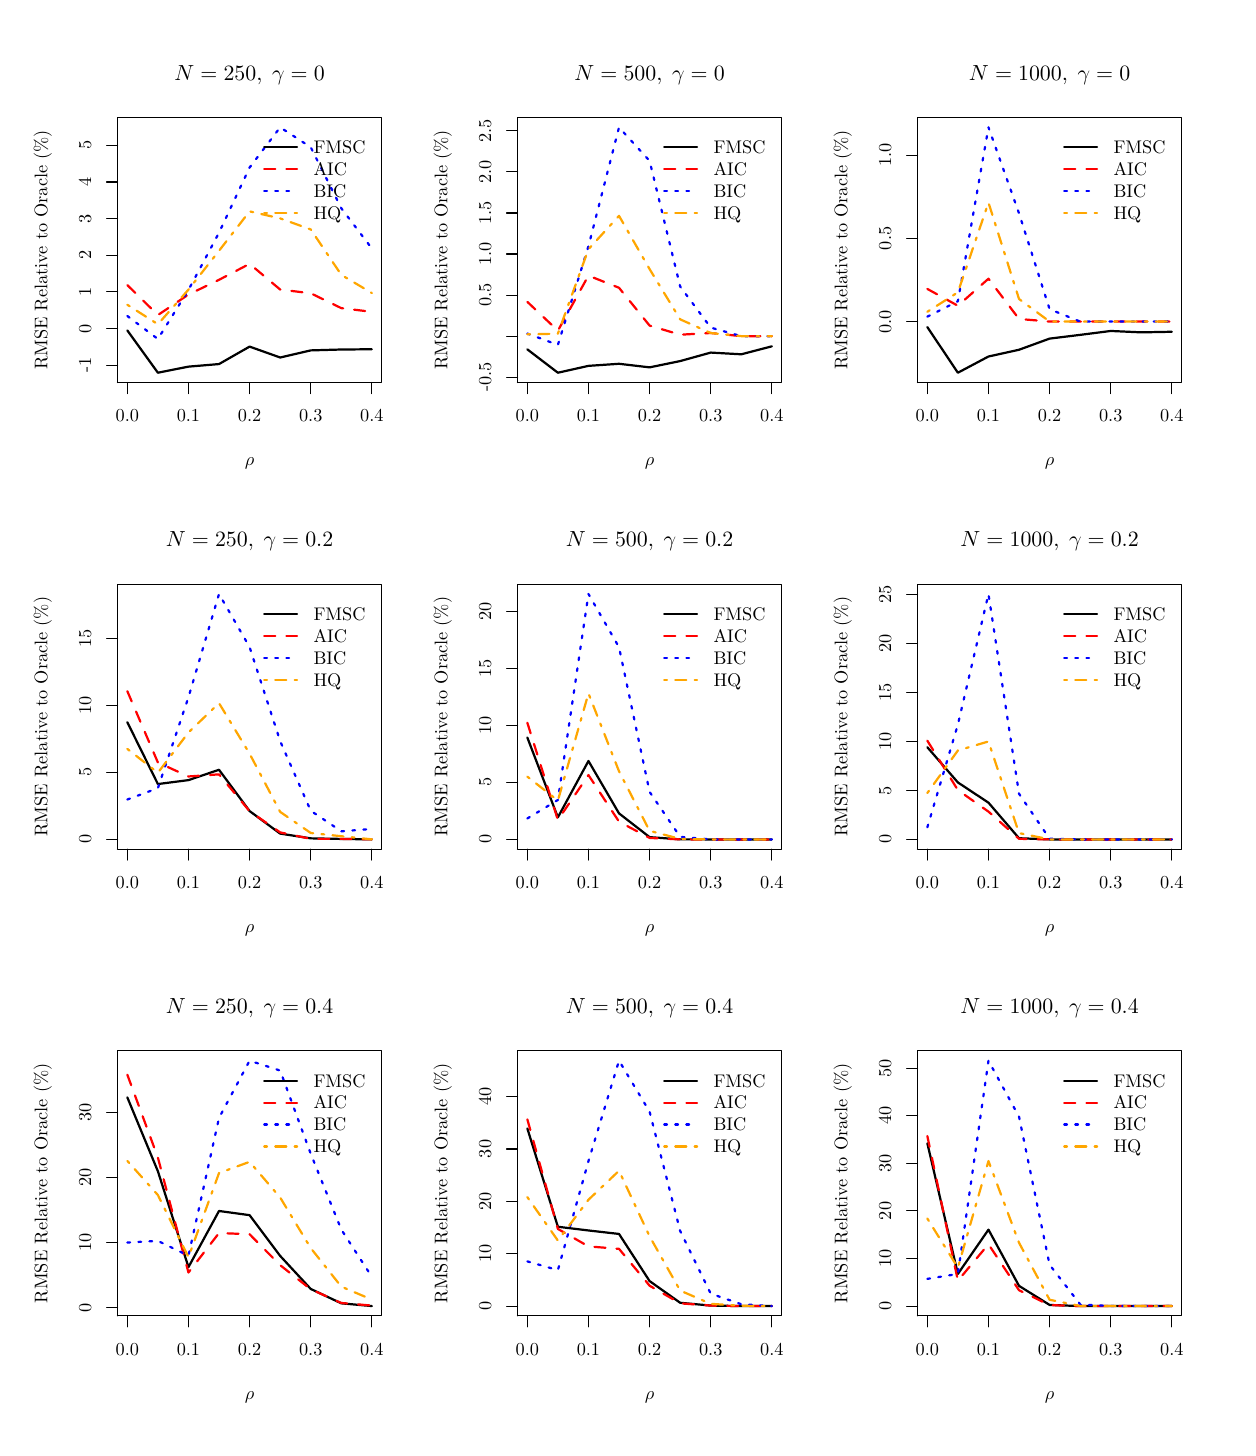
\begin{tikzpicture}[x=1pt,y=1pt]
\definecolor[named]{fillColor}{rgb}{1.00,1.00,1.00}
\path[use as bounding box,fill=fillColor,fill opacity=0.00] (0,0) rectangle (433.62,505.89);
\begin{scope}
\path[clip] ( 32.47,377.65) rectangle (127.91,473.42);
\definecolor[named]{drawColor}{rgb}{0.00,0.00,0.00}

\path[draw=drawColor,line width= 0.8pt,line join=round,line cap=round] ( 36.01,396.49) --
	( 47.05,381.20) --
	( 58.10,383.40) --
	( 69.14,384.33) --
	( 80.19,390.64) --
	( 91.24,386.70) --
	(102.28,389.27) --
	(113.33,389.59) --
	(124.37,389.68);
\end{scope}
\begin{scope}
\path[clip] (  0.00,  0.00) rectangle (433.62,505.89);
\definecolor[named]{drawColor}{rgb}{0.00,0.00,0.00}

\path[draw=drawColor,line width= 0.4pt,line join=round,line cap=round] ( 36.01,377.65) -- (124.37,377.65);

\path[draw=drawColor,line width= 0.4pt,line join=round,line cap=round] ( 36.01,377.65) -- ( 36.01,373.69);

\path[draw=drawColor,line width= 0.4pt,line join=round,line cap=round] ( 58.10,377.65) -- ( 58.10,373.69);

\path[draw=drawColor,line width= 0.4pt,line join=round,line cap=round] ( 80.19,377.65) -- ( 80.19,373.69);

\path[draw=drawColor,line width= 0.4pt,line join=round,line cap=round] (102.28,377.65) -- (102.28,373.69);

\path[draw=drawColor,line width= 0.4pt,line join=round,line cap=round] (124.37,377.65) -- (124.37,373.69);

\node[text=drawColor,anchor=base,inner sep=0pt, outer sep=0pt, scale=  0.66] at ( 36.01,363.40) {0.0};

\node[text=drawColor,anchor=base,inner sep=0pt, outer sep=0pt, scale=  0.66] at ( 58.10,363.40) {0.1};

\node[text=drawColor,anchor=base,inner sep=0pt, outer sep=0pt, scale=  0.66] at ( 80.19,363.40) {0.2};

\node[text=drawColor,anchor=base,inner sep=0pt, outer sep=0pt, scale=  0.66] at (102.28,363.40) {0.3};

\node[text=drawColor,anchor=base,inner sep=0pt, outer sep=0pt, scale=  0.66] at (124.37,363.40) {0.4};

\path[draw=drawColor,line width= 0.4pt,line join=round,line cap=round] ( 32.47,383.95) -- ( 32.47,463.36);

\path[draw=drawColor,line width= 0.4pt,line join=round,line cap=round] ( 32.47,383.95) -- ( 28.51,383.95);

\path[draw=drawColor,line width= 0.4pt,line join=round,line cap=round] ( 32.47,397.19) -- ( 28.51,397.19);

\path[draw=drawColor,line width= 0.4pt,line join=round,line cap=round] ( 32.47,410.42) -- ( 28.51,410.42);

\path[draw=drawColor,line width= 0.4pt,line join=round,line cap=round] ( 32.47,423.66) -- ( 28.51,423.66);

\path[draw=drawColor,line width= 0.4pt,line join=round,line cap=round] ( 32.47,436.89) -- ( 28.51,436.89);

\path[draw=drawColor,line width= 0.4pt,line join=round,line cap=round] ( 32.47,450.12) -- ( 28.51,450.12);

\path[draw=drawColor,line width= 0.4pt,line join=round,line cap=round] ( 32.47,463.36) -- ( 28.51,463.36);

\node[text=drawColor,rotate= 90.00,anchor=base,inner sep=0pt, outer sep=0pt, scale=  0.66] at ( 22.97,383.95) {-1};

\node[text=drawColor,rotate= 90.00,anchor=base,inner sep=0pt, outer sep=0pt, scale=  0.66] at ( 22.97,397.19) {0};

\node[text=drawColor,rotate= 90.00,anchor=base,inner sep=0pt, outer sep=0pt, scale=  0.66] at ( 22.97,410.42) {1};

\node[text=drawColor,rotate= 90.00,anchor=base,inner sep=0pt, outer sep=0pt, scale=  0.66] at ( 22.97,423.66) {2};

\node[text=drawColor,rotate= 90.00,anchor=base,inner sep=0pt, outer sep=0pt, scale=  0.66] at ( 22.97,436.89) {3};

\node[text=drawColor,rotate= 90.00,anchor=base,inner sep=0pt, outer sep=0pt, scale=  0.66] at ( 22.97,450.12) {4};

\node[text=drawColor,rotate= 90.00,anchor=base,inner sep=0pt, outer sep=0pt, scale=  0.66] at ( 22.97,463.36) {5};

\path[draw=drawColor,line width= 0.4pt,line join=round,line cap=round] ( 32.47,377.65) --
	(127.91,377.65) --
	(127.91,473.42) --
	( 32.47,473.42) --
	( 32.47,377.65);
\end{scope}
\begin{scope}
\path[clip] (  0.00,337.26) rectangle (144.54,505.89);
\definecolor[named]{drawColor}{rgb}{0.00,0.00,0.00}

\node[text=drawColor,anchor=base,inner sep=0pt, outer sep=0pt, scale=  0.79] at ( 80.19,486.92) {\bfseries $N=250, \;\gamma=0$};

\node[text=drawColor,anchor=base,inner sep=0pt, outer sep=0pt, scale=  0.66] at ( 80.19,347.56) {$\rho$};

\node[text=drawColor,rotate= 90.00,anchor=base,inner sep=0pt, outer sep=0pt, scale=  0.66] at (  7.13,425.53) {RMSE Relative to Oracle (\%)};
\end{scope}
\begin{scope}
\path[clip] ( 32.47,377.65) rectangle (127.91,473.42);
\definecolor[named]{drawColor}{rgb}{1.00,0.00,0.00}

\path[draw=drawColor,line width= 0.8pt,dash pattern=on 4pt off 4pt ,line join=round,line cap=round] ( 36.01,412.87) --
	( 47.05,402.05) --
	( 58.10,409.44) --
	( 69.14,414.77) --
	( 80.19,420.55) --
	( 91.24,411.26) --
	(102.28,409.91) --
	(113.33,404.54) --
	(124.37,403.21);
\definecolor[named]{drawColor}{rgb}{0.00,0.00,1.00}

\path[draw=drawColor,line width= 0.8pt,dash pattern=on 1pt off 3pt ,line join=round,line cap=round] ( 36.01,401.70) --
	( 47.05,393.38) --
	( 58.10,411.10) --
	( 69.14,431.79) --
	( 80.19,455.35) --
	( 91.24,469.87) --
	(102.28,462.69) --
	(113.33,440.62) --
	(124.37,426.10);
\definecolor[named]{drawColor}{rgb}{1.00,0.65,0.00}

\path[draw=drawColor,line width= 0.8pt,dash pattern=on 1pt off 3pt on 4pt off 3pt ,line join=round,line cap=round] ( 36.01,405.76) --
	( 47.05,398.72) --
	( 58.10,411.22) --
	( 69.14,425.26) --
	( 80.19,439.51) --
	( 91.24,436.97) --
	(102.28,432.98) --
	(113.33,416.56) --
	(124.37,409.99);
\definecolor[named]{drawColor}{rgb}{0.00,0.00,0.00}

\path[draw=drawColor,line width= 0.8pt,line join=round,line cap=round] ( 85.47,462.63) -- ( 97.35,462.63);
\definecolor[named]{drawColor}{rgb}{1.00,0.00,0.00}

\path[draw=drawColor,line width= 0.8pt,dash pattern=on 4pt off 4pt ,line join=round,line cap=round] ( 85.47,454.71) -- ( 97.35,454.71);
\definecolor[named]{drawColor}{rgb}{0.00,0.00,1.00}

\path[draw=drawColor,line width= 0.8pt,dash pattern=on 1pt off 3pt ,line join=round,line cap=round] ( 85.47,446.79) -- ( 97.35,446.79);
\definecolor[named]{drawColor}{rgb}{1.00,0.65,0.00}

\path[draw=drawColor,line width= 0.8pt,dash pattern=on 1pt off 3pt on 4pt off 3pt ,line join=round,line cap=round] ( 85.47,438.87) -- ( 97.35,438.87);
\definecolor[named]{drawColor}{rgb}{0.00,0.00,0.00}

\node[text=drawColor,anchor=base west,inner sep=0pt, outer sep=0pt, scale=  0.66] at (103.29,460.35) {FMSC};

\node[text=drawColor,anchor=base west,inner sep=0pt, outer sep=0pt, scale=  0.66] at (103.29,452.43) {AIC};

\node[text=drawColor,anchor=base west,inner sep=0pt, outer sep=0pt, scale=  0.66] at (103.29,444.51) {BIC};

\node[text=drawColor,anchor=base west,inner sep=0pt, outer sep=0pt, scale=  0.66] at (103.29,436.59) {HQ};
\end{scope}
\begin{scope}
\path[clip] (177.01,377.65) rectangle (272.45,473.42);
\definecolor[named]{drawColor}{rgb}{0.00,0.00,0.00}

\path[draw=drawColor,line width= 0.8pt,line join=round,line cap=round] (180.55,389.64) --
	(191.59,381.20) --
	(202.64,383.68) --
	(213.68,384.43) --
	(224.73,383.14) --
	(235.78,385.41) --
	(246.82,388.48) --
	(257.87,387.86) --
	(268.91,390.74);
\end{scope}
\begin{scope}
\path[clip] (  0.00,  0.00) rectangle (433.62,505.89);
\definecolor[named]{drawColor}{rgb}{0.00,0.00,0.00}

\path[draw=drawColor,line width= 0.4pt,line join=round,line cap=round] (180.55,377.65) -- (268.91,377.65);

\path[draw=drawColor,line width= 0.4pt,line join=round,line cap=round] (180.55,377.65) -- (180.55,373.69);

\path[draw=drawColor,line width= 0.4pt,line join=round,line cap=round] (202.64,377.65) -- (202.64,373.69);

\path[draw=drawColor,line width= 0.4pt,line join=round,line cap=round] (224.73,377.65) -- (224.73,373.69);

\path[draw=drawColor,line width= 0.4pt,line join=round,line cap=round] (246.82,377.65) -- (246.82,373.69);

\path[draw=drawColor,line width= 0.4pt,line join=round,line cap=round] (268.91,377.65) -- (268.91,373.69);

\node[text=drawColor,anchor=base,inner sep=0pt, outer sep=0pt, scale=  0.66] at (180.55,363.40) {0.0};

\node[text=drawColor,anchor=base,inner sep=0pt, outer sep=0pt, scale=  0.66] at (202.64,363.40) {0.1};

\node[text=drawColor,anchor=base,inner sep=0pt, outer sep=0pt, scale=  0.66] at (224.73,363.40) {0.2};

\node[text=drawColor,anchor=base,inner sep=0pt, outer sep=0pt, scale=  0.66] at (246.82,363.40) {0.3};

\node[text=drawColor,anchor=base,inner sep=0pt, outer sep=0pt, scale=  0.66] at (268.91,363.40) {0.4};

\path[draw=drawColor,line width= 0.4pt,line join=round,line cap=round] (177.01,379.57) -- (177.01,468.61);

\path[draw=drawColor,line width= 0.4pt,line join=round,line cap=round] (177.01,379.57) -- (173.05,379.57);

\path[draw=drawColor,line width= 0.4pt,line join=round,line cap=round] (177.01,394.41) -- (173.05,394.41);

\path[draw=drawColor,line width= 0.4pt,line join=round,line cap=round] (177.01,409.25) -- (173.05,409.25);

\path[draw=drawColor,line width= 0.4pt,line join=round,line cap=round] (177.01,424.09) -- (173.05,424.09);

\path[draw=drawColor,line width= 0.4pt,line join=round,line cap=round] (177.01,438.93) -- (173.05,438.93);

\path[draw=drawColor,line width= 0.4pt,line join=round,line cap=round] (177.01,453.77) -- (173.05,453.77);

\path[draw=drawColor,line width= 0.4pt,line join=round,line cap=round] (177.01,468.61) -- (173.05,468.61);

\node[text=drawColor,rotate= 90.00,anchor=base,inner sep=0pt, outer sep=0pt, scale=  0.66] at (167.51,379.57) {-0.5};

\node[text=drawColor,rotate= 90.00,anchor=base,inner sep=0pt, outer sep=0pt, scale=  0.66] at (167.51,409.25) {0.5};

\node[text=drawColor,rotate= 90.00,anchor=base,inner sep=0pt, outer sep=0pt, scale=  0.66] at (167.51,424.09) {1.0};

\node[text=drawColor,rotate= 90.00,anchor=base,inner sep=0pt, outer sep=0pt, scale=  0.66] at (167.51,438.93) {1.5};

\node[text=drawColor,rotate= 90.00,anchor=base,inner sep=0pt, outer sep=0pt, scale=  0.66] at (167.51,453.77) {2.0};

\node[text=drawColor,rotate= 90.00,anchor=base,inner sep=0pt, outer sep=0pt, scale=  0.66] at (167.51,468.61) {2.5};

\path[draw=drawColor,line width= 0.4pt,line join=round,line cap=round] (177.01,377.65) --
	(272.45,377.65) --
	(272.45,473.42) --
	(177.01,473.42) --
	(177.01,377.65);
\end{scope}
\begin{scope}
\path[clip] (144.54,337.26) rectangle (289.08,505.89);
\definecolor[named]{drawColor}{rgb}{0.00,0.00,0.00}

\node[text=drawColor,anchor=base,inner sep=0pt, outer sep=0pt, scale=  0.79] at (224.73,486.92) {\bfseries $N=500, \;\gamma=0$};

\node[text=drawColor,anchor=base,inner sep=0pt, outer sep=0pt, scale=  0.66] at (224.73,347.56) {$\rho$};

\node[text=drawColor,rotate= 90.00,anchor=base,inner sep=0pt, outer sep=0pt, scale=  0.66] at (151.67,425.53) {RMSE Relative to Oracle (\%)};
\end{scope}
\begin{scope}
\path[clip] (177.01,377.65) rectangle (272.45,473.42);
\definecolor[named]{drawColor}{rgb}{1.00,0.00,0.00}

\path[draw=drawColor,line width= 0.8pt,dash pattern=on 4pt off 4pt ,line join=round,line cap=round] (180.55,406.81) --
	(191.59,396.39) --
	(202.64,416.29) --
	(213.68,411.89) --
	(224.73,398.23) --
	(235.78,394.94) --
	(246.82,395.55) --
	(257.87,394.41) --
	(268.91,394.41);
\definecolor[named]{drawColor}{rgb}{0.00,0.00,1.00}

\path[draw=drawColor,line width= 0.8pt,dash pattern=on 1pt off 3pt ,line join=round,line cap=round] (180.55,395.37) --
	(191.59,391.25) --
	(202.64,426.93) --
	(213.68,469.87) --
	(224.73,457.75) --
	(235.78,412.35) --
	(246.82,397.50) --
	(257.87,394.41) --
	(268.91,394.41);
\definecolor[named]{drawColor}{rgb}{1.00,0.65,0.00}

\path[draw=drawColor,line width= 0.8pt,dash pattern=on 1pt off 3pt on 4pt off 3pt ,line join=round,line cap=round] (180.55,395.07) --
	(191.59,395.31) --
	(202.64,425.84) --
	(213.68,437.89) --
	(224.73,418.64) --
	(235.78,400.49) --
	(246.82,395.55) --
	(257.87,394.41) --
	(268.91,394.41);
\definecolor[named]{drawColor}{rgb}{0.00,0.00,0.00}

\path[draw=drawColor,line width= 0.8pt,line join=round,line cap=round] (230.01,462.63) -- (241.89,462.63);
\definecolor[named]{drawColor}{rgb}{1.00,0.00,0.00}

\path[draw=drawColor,line width= 0.8pt,dash pattern=on 4pt off 4pt ,line join=round,line cap=round] (230.01,454.71) -- (241.89,454.71);
\definecolor[named]{drawColor}{rgb}{0.00,0.00,1.00}

\path[draw=drawColor,line width= 0.8pt,dash pattern=on 1pt off 3pt ,line join=round,line cap=round] (230.01,446.79) -- (241.89,446.79);
\definecolor[named]{drawColor}{rgb}{1.00,0.65,0.00}

\path[draw=drawColor,line width= 0.8pt,dash pattern=on 1pt off 3pt on 4pt off 3pt ,line join=round,line cap=round] (230.01,438.87) -- (241.89,438.87);
\definecolor[named]{drawColor}{rgb}{0.00,0.00,0.00}

\node[text=drawColor,anchor=base west,inner sep=0pt, outer sep=0pt, scale=  0.66] at (247.83,460.35) {FMSC};

\node[text=drawColor,anchor=base west,inner sep=0pt, outer sep=0pt, scale=  0.66] at (247.83,452.43) {AIC};

\node[text=drawColor,anchor=base west,inner sep=0pt, outer sep=0pt, scale=  0.66] at (247.83,444.51) {BIC};

\node[text=drawColor,anchor=base west,inner sep=0pt, outer sep=0pt, scale=  0.66] at (247.83,436.59) {HQ};
\end{scope}
\begin{scope}
\path[clip] (321.55,377.65) rectangle (416.99,473.42);
\definecolor[named]{drawColor}{rgb}{0.00,0.00,0.00}

\path[draw=drawColor,line width= 0.8pt,line join=round,line cap=round] (325.09,397.69) --
	(336.13,381.20) --
	(347.18,387.06) --
	(358.22,389.50) --
	(369.27,393.53) --
	(380.32,394.88) --
	(391.36,396.29) --
	(402.41,395.79) --
	(413.45,396.00);
\end{scope}
\begin{scope}
\path[clip] (  0.00,  0.00) rectangle (433.62,505.89);
\definecolor[named]{drawColor}{rgb}{0.00,0.00,0.00}

\path[draw=drawColor,line width= 0.4pt,line join=round,line cap=round] (325.09,377.65) -- (413.45,377.65);

\path[draw=drawColor,line width= 0.4pt,line join=round,line cap=round] (325.09,377.65) -- (325.09,373.69);

\path[draw=drawColor,line width= 0.4pt,line join=round,line cap=round] (347.18,377.65) -- (347.18,373.69);

\path[draw=drawColor,line width= 0.4pt,line join=round,line cap=round] (369.27,377.65) -- (369.27,373.69);

\path[draw=drawColor,line width= 0.4pt,line join=round,line cap=round] (391.36,377.65) -- (391.36,373.69);

\path[draw=drawColor,line width= 0.4pt,line join=round,line cap=round] (413.45,377.65) -- (413.45,373.69);

\node[text=drawColor,anchor=base,inner sep=0pt, outer sep=0pt, scale=  0.66] at (325.09,363.40) {0.0};

\node[text=drawColor,anchor=base,inner sep=0pt, outer sep=0pt, scale=  0.66] at (347.18,363.40) {0.1};

\node[text=drawColor,anchor=base,inner sep=0pt, outer sep=0pt, scale=  0.66] at (369.27,363.40) {0.2};

\node[text=drawColor,anchor=base,inner sep=0pt, outer sep=0pt, scale=  0.66] at (391.36,363.40) {0.3};

\node[text=drawColor,anchor=base,inner sep=0pt, outer sep=0pt, scale=  0.66] at (413.45,363.40) {0.4};

\path[draw=drawColor,line width= 0.4pt,line join=round,line cap=round] (321.55,399.69) -- (321.55,459.81);

\path[draw=drawColor,line width= 0.4pt,line join=round,line cap=round] (321.55,399.69) -- (317.59,399.69);

\path[draw=drawColor,line width= 0.4pt,line join=round,line cap=round] (321.55,429.75) -- (317.59,429.75);

\path[draw=drawColor,line width= 0.4pt,line join=round,line cap=round] (321.55,459.81) -- (317.59,459.81);

\node[text=drawColor,rotate= 90.00,anchor=base,inner sep=0pt, outer sep=0pt, scale=  0.66] at (312.05,399.69) {0.0};

\node[text=drawColor,rotate= 90.00,anchor=base,inner sep=0pt, outer sep=0pt, scale=  0.66] at (312.05,429.75) {0.5};

\node[text=drawColor,rotate= 90.00,anchor=base,inner sep=0pt, outer sep=0pt, scale=  0.66] at (312.05,459.81) {1.0};

\path[draw=drawColor,line width= 0.4pt,line join=round,line cap=round] (321.55,377.65) --
	(416.99,377.65) --
	(416.99,473.42) --
	(321.55,473.42) --
	(321.55,377.65);
\end{scope}
\begin{scope}
\path[clip] (289.08,337.26) rectangle (433.62,505.89);
\definecolor[named]{drawColor}{rgb}{0.00,0.00,0.00}

\node[text=drawColor,anchor=base,inner sep=0pt, outer sep=0pt, scale=  0.79] at (369.27,486.92) {\bfseries $N=1000, \;\gamma=0$};

\node[text=drawColor,anchor=base,inner sep=0pt, outer sep=0pt, scale=  0.66] at (369.27,347.56) {$\rho$};

\node[text=drawColor,rotate= 90.00,anchor=base,inner sep=0pt, outer sep=0pt, scale=  0.66] at (296.21,425.53) {RMSE Relative to Oracle (\%)};
\end{scope}
\begin{scope}
\path[clip] (321.55,377.65) rectangle (416.99,473.42);
\definecolor[named]{drawColor}{rgb}{1.00,0.00,0.00}

\path[draw=drawColor,line width= 0.8pt,dash pattern=on 4pt off 4pt ,line join=round,line cap=round] (325.09,411.48) --
	(336.13,405.40) --
	(347.18,415.17) --
	(358.22,400.63) --
	(369.27,399.69) --
	(380.32,399.69) --
	(391.36,399.69) --
	(402.41,399.69) --
	(413.45,399.69);
\definecolor[named]{drawColor}{rgb}{0.00,0.00,1.00}

\path[draw=drawColor,line width= 0.8pt,dash pattern=on 1pt off 3pt ,line join=round,line cap=round] (325.09,401.45) --
	(336.13,407.03) --
	(347.18,469.87) --
	(358.22,438.81) --
	(369.27,404.16) --
	(380.32,399.69) --
	(391.36,399.69) --
	(402.41,399.69) --
	(413.45,399.69);
\definecolor[named]{drawColor}{rgb}{1.00,0.65,0.00}

\path[draw=drawColor,line width= 0.8pt,dash pattern=on 1pt off 3pt on 4pt off 3pt ,line join=round,line cap=round] (325.09,403.22) --
	(336.13,410.25) --
	(347.18,442.68) --
	(358.22,407.84) --
	(369.27,399.69) --
	(380.32,399.69) --
	(391.36,399.69) --
	(402.41,399.69) --
	(413.45,399.69);
\definecolor[named]{drawColor}{rgb}{0.00,0.00,0.00}

\path[draw=drawColor,line width= 0.8pt,line join=round,line cap=round] (374.55,462.63) -- (386.43,462.63);
\definecolor[named]{drawColor}{rgb}{1.00,0.00,0.00}

\path[draw=drawColor,line width= 0.8pt,dash pattern=on 4pt off 4pt ,line join=round,line cap=round] (374.55,454.71) -- (386.43,454.71);
\definecolor[named]{drawColor}{rgb}{0.00,0.00,1.00}

\path[draw=drawColor,line width= 0.8pt,dash pattern=on 1pt off 3pt ,line join=round,line cap=round] (374.55,446.79) -- (386.43,446.79);
\definecolor[named]{drawColor}{rgb}{1.00,0.65,0.00}

\path[draw=drawColor,line width= 0.8pt,dash pattern=on 1pt off 3pt on 4pt off 3pt ,line join=round,line cap=round] (374.55,438.87) -- (386.43,438.87);
\definecolor[named]{drawColor}{rgb}{0.00,0.00,0.00}

\node[text=drawColor,anchor=base west,inner sep=0pt, outer sep=0pt, scale=  0.66] at (392.37,460.35) {FMSC};

\node[text=drawColor,anchor=base west,inner sep=0pt, outer sep=0pt, scale=  0.66] at (392.37,452.43) {AIC};

\node[text=drawColor,anchor=base west,inner sep=0pt, outer sep=0pt, scale=  0.66] at (392.37,444.51) {BIC};

\node[text=drawColor,anchor=base west,inner sep=0pt, outer sep=0pt, scale=  0.66] at (392.37,436.59) {HQ};
\end{scope}
\begin{scope}
\path[clip] ( 32.47,209.02) rectangle (127.91,304.79);
\definecolor[named]{drawColor}{rgb}{0.00,0.00,0.00}

\path[draw=drawColor,line width= 0.8pt,line join=round,line cap=round] ( 36.01,254.91) --
	( 47.05,232.57) --
	( 58.10,233.99) --
	( 69.14,237.73) --
	( 80.19,222.81) --
	( 91.24,214.66) --
	(102.28,212.95) --
	(113.33,212.74) --
	(124.37,212.57);
\end{scope}
\begin{scope}
\path[clip] (  0.00,  0.00) rectangle (433.62,505.89);
\definecolor[named]{drawColor}{rgb}{0.00,0.00,0.00}

\path[draw=drawColor,line width= 0.4pt,line join=round,line cap=round] ( 36.01,209.02) -- (124.37,209.02);

\path[draw=drawColor,line width= 0.4pt,line join=round,line cap=round] ( 36.01,209.02) -- ( 36.01,205.06);

\path[draw=drawColor,line width= 0.4pt,line join=round,line cap=round] ( 58.10,209.02) -- ( 58.10,205.06);

\path[draw=drawColor,line width= 0.4pt,line join=round,line cap=round] ( 80.19,209.02) -- ( 80.19,205.06);

\path[draw=drawColor,line width= 0.4pt,line join=round,line cap=round] (102.28,209.02) -- (102.28,205.06);

\path[draw=drawColor,line width= 0.4pt,line join=round,line cap=round] (124.37,209.02) -- (124.37,205.06);

\node[text=drawColor,anchor=base,inner sep=0pt, outer sep=0pt, scale=  0.66] at ( 36.01,194.77) {0.0};

\node[text=drawColor,anchor=base,inner sep=0pt, outer sep=0pt, scale=  0.66] at ( 58.10,194.77) {0.1};

\node[text=drawColor,anchor=base,inner sep=0pt, outer sep=0pt, scale=  0.66] at ( 80.19,194.77) {0.2};

\node[text=drawColor,anchor=base,inner sep=0pt, outer sep=0pt, scale=  0.66] at (102.28,194.77) {0.3};

\node[text=drawColor,anchor=base,inner sep=0pt, outer sep=0pt, scale=  0.66] at (124.37,194.77) {0.4};

\path[draw=drawColor,line width= 0.4pt,line join=round,line cap=round] ( 32.47,212.59) -- ( 32.47,285.16);

\path[draw=drawColor,line width= 0.4pt,line join=round,line cap=round] ( 32.47,212.59) -- ( 28.51,212.59);

\path[draw=drawColor,line width= 0.4pt,line join=round,line cap=round] ( 32.47,236.78) -- ( 28.51,236.78);

\path[draw=drawColor,line width= 0.4pt,line join=round,line cap=round] ( 32.47,260.97) -- ( 28.51,260.97);

\path[draw=drawColor,line width= 0.4pt,line join=round,line cap=round] ( 32.47,285.16) -- ( 28.51,285.16);

\node[text=drawColor,rotate= 90.00,anchor=base,inner sep=0pt, outer sep=0pt, scale=  0.66] at ( 22.97,212.59) {0};

\node[text=drawColor,rotate= 90.00,anchor=base,inner sep=0pt, outer sep=0pt, scale=  0.66] at ( 22.97,236.78) {5};

\node[text=drawColor,rotate= 90.00,anchor=base,inner sep=0pt, outer sep=0pt, scale=  0.66] at ( 22.97,260.97) {10};

\node[text=drawColor,rotate= 90.00,anchor=base,inner sep=0pt, outer sep=0pt, scale=  0.66] at ( 22.97,285.16) {15};

\path[draw=drawColor,line width= 0.4pt,line join=round,line cap=round] ( 32.47,209.02) --
	(127.91,209.02) --
	(127.91,304.79) --
	( 32.47,304.79) --
	( 32.47,209.02);
\end{scope}
\begin{scope}
\path[clip] (  0.00,168.63) rectangle (144.54,337.26);
\definecolor[named]{drawColor}{rgb}{0.00,0.00,0.00}

\node[text=drawColor,anchor=base,inner sep=0pt, outer sep=0pt, scale=  0.79] at ( 80.19,318.29) {\bfseries $N=250, \;\gamma=0.2$};

\node[text=drawColor,anchor=base,inner sep=0pt, outer sep=0pt, scale=  0.66] at ( 80.19,178.93) {$\rho$};

\node[text=drawColor,rotate= 90.00,anchor=base,inner sep=0pt, outer sep=0pt, scale=  0.66] at (  7.13,256.90) {RMSE Relative to Oracle (\%)};
\end{scope}
\begin{scope}
\path[clip] ( 32.47,209.02) rectangle (127.91,304.79);
\definecolor[named]{drawColor}{rgb}{1.00,0.00,0.00}

\path[draw=drawColor,line width= 0.8pt,dash pattern=on 4pt off 4pt ,line join=round,line cap=round] ( 36.01,266.12) --
	( 47.05,240.36) --
	( 58.10,235.31) --
	( 69.14,236.07) --
	( 80.19,222.76) --
	( 91.24,215.10) --
	(102.28,212.76) --
	(113.33,212.76) --
	(124.37,212.59);
\definecolor[named]{drawColor}{rgb}{0.00,0.00,1.00}

\path[draw=drawColor,line width= 0.8pt,dash pattern=on 1pt off 3pt ,line join=round,line cap=round] ( 36.01,226.98) --
	( 47.05,231.09) --
	( 58.10,263.94) --
	( 69.14,301.24) --
	( 80.19,282.08) --
	( 91.24,248.07) --
	(102.28,222.93) --
	(113.33,215.49) --
	(124.37,216.35);
\definecolor[named]{drawColor}{rgb}{1.00,0.65,0.00}

\path[draw=drawColor,line width= 0.8pt,dash pattern=on 1pt off 3pt on 4pt off 3pt ,line join=round,line cap=round] ( 36.01,245.26) --
	( 47.05,236.64) --
	( 58.10,251.20) --
	( 69.14,261.81) --
	( 80.19,243.54) --
	( 91.24,222.52) --
	(102.28,214.89) --
	(113.33,213.72) --
	(124.37,212.59);
\definecolor[named]{drawColor}{rgb}{0.00,0.00,0.00}

\path[draw=drawColor,line width= 0.8pt,line join=round,line cap=round] ( 85.47,294.00) -- ( 97.35,294.00);
\definecolor[named]{drawColor}{rgb}{1.00,0.00,0.00}

\path[draw=drawColor,line width= 0.8pt,dash pattern=on 4pt off 4pt ,line join=round,line cap=round] ( 85.47,286.08) -- ( 97.35,286.08);
\definecolor[named]{drawColor}{rgb}{0.00,0.00,1.00}

\path[draw=drawColor,line width= 0.8pt,dash pattern=on 1pt off 3pt ,line join=round,line cap=round] ( 85.47,278.16) -- ( 97.35,278.16);
\definecolor[named]{drawColor}{rgb}{1.00,0.65,0.00}

\path[draw=drawColor,line width= 0.8pt,dash pattern=on 1pt off 3pt on 4pt off 3pt ,line join=round,line cap=round] ( 85.47,270.24) -- ( 97.35,270.24);
\definecolor[named]{drawColor}{rgb}{0.00,0.00,0.00}

\node[text=drawColor,anchor=base west,inner sep=0pt, outer sep=0pt, scale=  0.66] at (103.29,291.72) {FMSC};

\node[text=drawColor,anchor=base west,inner sep=0pt, outer sep=0pt, scale=  0.66] at (103.29,283.80) {AIC};

\node[text=drawColor,anchor=base west,inner sep=0pt, outer sep=0pt, scale=  0.66] at (103.29,275.88) {BIC};

\node[text=drawColor,anchor=base west,inner sep=0pt, outer sep=0pt, scale=  0.66] at (103.29,267.96) {HQ};
\end{scope}
\begin{scope}
\path[clip] (177.01,209.02) rectangle (272.45,304.79);
\definecolor[named]{drawColor}{rgb}{0.00,0.00,0.00}

\path[draw=drawColor,line width= 0.8pt,line join=round,line cap=round] (180.55,249.38) --
	(191.59,220.54) --
	(202.64,240.91) --
	(213.68,221.97) --
	(224.73,213.39) --
	(235.78,212.58) --
	(246.82,212.57) --
	(257.87,212.57) --
	(268.91,212.57);
\end{scope}
\begin{scope}
\path[clip] (  0.00,  0.00) rectangle (433.62,505.89);
\definecolor[named]{drawColor}{rgb}{0.00,0.00,0.00}

\path[draw=drawColor,line width= 0.4pt,line join=round,line cap=round] (180.55,209.02) -- (268.91,209.02);

\path[draw=drawColor,line width= 0.4pt,line join=round,line cap=round] (180.55,209.02) -- (180.55,205.06);

\path[draw=drawColor,line width= 0.4pt,line join=round,line cap=round] (202.64,209.02) -- (202.64,205.06);

\path[draw=drawColor,line width= 0.4pt,line join=round,line cap=round] (224.73,209.02) -- (224.73,205.06);

\path[draw=drawColor,line width= 0.4pt,line join=round,line cap=round] (246.82,209.02) -- (246.82,205.06);

\path[draw=drawColor,line width= 0.4pt,line join=round,line cap=round] (268.91,209.02) -- (268.91,205.06);

\node[text=drawColor,anchor=base,inner sep=0pt, outer sep=0pt, scale=  0.66] at (180.55,194.77) {0.0};

\node[text=drawColor,anchor=base,inner sep=0pt, outer sep=0pt, scale=  0.66] at (202.64,194.77) {0.1};

\node[text=drawColor,anchor=base,inner sep=0pt, outer sep=0pt, scale=  0.66] at (224.73,194.77) {0.2};

\node[text=drawColor,anchor=base,inner sep=0pt, outer sep=0pt, scale=  0.66] at (246.82,194.77) {0.3};

\node[text=drawColor,anchor=base,inner sep=0pt, outer sep=0pt, scale=  0.66] at (268.91,194.77) {0.4};

\path[draw=drawColor,line width= 0.4pt,line join=round,line cap=round] (177.01,212.57) -- (177.01,295.01);

\path[draw=drawColor,line width= 0.4pt,line join=round,line cap=round] (177.01,212.57) -- (173.05,212.57);

\path[draw=drawColor,line width= 0.4pt,line join=round,line cap=round] (177.01,233.18) -- (173.05,233.18);

\path[draw=drawColor,line width= 0.4pt,line join=round,line cap=round] (177.01,253.79) -- (173.05,253.79);

\path[draw=drawColor,line width= 0.4pt,line join=round,line cap=round] (177.01,274.40) -- (173.05,274.40);

\path[draw=drawColor,line width= 0.4pt,line join=round,line cap=round] (177.01,295.01) -- (173.05,295.01);

\node[text=drawColor,rotate= 90.00,anchor=base,inner sep=0pt, outer sep=0pt, scale=  0.66] at (167.51,212.57) {0};

\node[text=drawColor,rotate= 90.00,anchor=base,inner sep=0pt, outer sep=0pt, scale=  0.66] at (167.51,233.18) {5};

\node[text=drawColor,rotate= 90.00,anchor=base,inner sep=0pt, outer sep=0pt, scale=  0.66] at (167.51,253.79) {10};

\node[text=drawColor,rotate= 90.00,anchor=base,inner sep=0pt, outer sep=0pt, scale=  0.66] at (167.51,274.40) {15};

\node[text=drawColor,rotate= 90.00,anchor=base,inner sep=0pt, outer sep=0pt, scale=  0.66] at (167.51,295.01) {20};

\path[draw=drawColor,line width= 0.4pt,line join=round,line cap=round] (177.01,209.02) --
	(272.45,209.02) --
	(272.45,304.79) --
	(177.01,304.79) --
	(177.01,209.02);
\end{scope}
\begin{scope}
\path[clip] (144.54,168.63) rectangle (289.08,337.26);
\definecolor[named]{drawColor}{rgb}{0.00,0.00,0.00}

\node[text=drawColor,anchor=base,inner sep=0pt, outer sep=0pt, scale=  0.79] at (224.73,318.29) {\bfseries $N=500, \;\gamma=0.2$};

\node[text=drawColor,anchor=base,inner sep=0pt, outer sep=0pt, scale=  0.66] at (224.73,178.93) {$\rho$};

\node[text=drawColor,rotate= 90.00,anchor=base,inner sep=0pt, outer sep=0pt, scale=  0.66] at (151.67,256.90) {RMSE Relative to Oracle (\%)};
\end{scope}
\begin{scope}
\path[clip] (177.01,209.02) rectangle (272.45,304.79);
\definecolor[named]{drawColor}{rgb}{1.00,0.00,0.00}

\path[draw=drawColor,line width= 0.8pt,dash pattern=on 4pt off 4pt ,line join=round,line cap=round] (180.55,254.72) --
	(191.59,219.59) --
	(202.64,235.82) --
	(213.68,218.97) --
	(224.73,213.10) --
	(235.78,212.57) --
	(246.82,212.57) --
	(257.87,212.57) --
	(268.91,212.57);
\definecolor[named]{drawColor}{rgb}{0.00,0.00,1.00}

\path[draw=drawColor,line width= 0.8pt,dash pattern=on 1pt off 3pt ,line join=round,line cap=round] (180.55,220.13) --
	(191.59,226.82) --
	(202.64,301.24) --
	(213.68,282.01) --
	(224.73,229.74) --
	(235.78,213.49) --
	(246.82,212.57) --
	(257.87,212.57) --
	(268.91,212.57);
\definecolor[named]{drawColor}{rgb}{1.00,0.65,0.00}

\path[draw=drawColor,line width= 0.8pt,dash pattern=on 1pt off 3pt on 4pt off 3pt ,line join=round,line cap=round] (180.55,235.25) --
	(191.59,226.61) --
	(202.64,265.34) --
	(213.68,237.18) --
	(224.73,215.66) --
	(235.78,212.74) --
	(246.82,212.57) --
	(257.87,212.57) --
	(268.91,212.57);
\definecolor[named]{drawColor}{rgb}{0.00,0.00,0.00}

\path[draw=drawColor,line width= 0.8pt,line join=round,line cap=round] (230.01,294.00) -- (241.89,294.00);
\definecolor[named]{drawColor}{rgb}{1.00,0.00,0.00}

\path[draw=drawColor,line width= 0.8pt,dash pattern=on 4pt off 4pt ,line join=round,line cap=round] (230.01,286.08) -- (241.89,286.08);
\definecolor[named]{drawColor}{rgb}{0.00,0.00,1.00}

\path[draw=drawColor,line width= 0.8pt,dash pattern=on 1pt off 3pt ,line join=round,line cap=round] (230.01,278.16) -- (241.89,278.16);
\definecolor[named]{drawColor}{rgb}{1.00,0.65,0.00}

\path[draw=drawColor,line width= 0.8pt,dash pattern=on 1pt off 3pt on 4pt off 3pt ,line join=round,line cap=round] (230.01,270.24) -- (241.89,270.24);
\definecolor[named]{drawColor}{rgb}{0.00,0.00,0.00}

\node[text=drawColor,anchor=base west,inner sep=0pt, outer sep=0pt, scale=  0.66] at (247.83,291.72) {FMSC};

\node[text=drawColor,anchor=base west,inner sep=0pt, outer sep=0pt, scale=  0.66] at (247.83,283.80) {AIC};

\node[text=drawColor,anchor=base west,inner sep=0pt, outer sep=0pt, scale=  0.66] at (247.83,275.88) {BIC};

\node[text=drawColor,anchor=base west,inner sep=0pt, outer sep=0pt, scale=  0.66] at (247.83,267.96) {HQ};
\end{scope}
\begin{scope}
\path[clip] (321.55,209.02) rectangle (416.99,304.79);
\definecolor[named]{drawColor}{rgb}{0.00,0.00,0.00}

\path[draw=drawColor,line width= 0.8pt,line join=round,line cap=round] (325.09,245.87) --
	(336.13,233.15) --
	(347.18,225.84) --
	(358.22,212.99) --
	(369.27,212.57) --
	(380.32,212.57) --
	(391.36,212.57) --
	(402.41,212.57) --
	(413.45,212.57);
\end{scope}
\begin{scope}
\path[clip] (  0.00,  0.00) rectangle (433.62,505.89);
\definecolor[named]{drawColor}{rgb}{0.00,0.00,0.00}

\path[draw=drawColor,line width= 0.4pt,line join=round,line cap=round] (325.09,209.02) -- (413.45,209.02);

\path[draw=drawColor,line width= 0.4pt,line join=round,line cap=round] (325.09,209.02) -- (325.09,205.06);

\path[draw=drawColor,line width= 0.4pt,line join=round,line cap=round] (347.18,209.02) -- (347.18,205.06);

\path[draw=drawColor,line width= 0.4pt,line join=round,line cap=round] (369.27,209.02) -- (369.27,205.06);

\path[draw=drawColor,line width= 0.4pt,line join=round,line cap=round] (391.36,209.02) -- (391.36,205.06);

\path[draw=drawColor,line width= 0.4pt,line join=round,line cap=round] (413.45,209.02) -- (413.45,205.06);

\node[text=drawColor,anchor=base,inner sep=0pt, outer sep=0pt, scale=  0.66] at (325.09,194.77) {0.0};

\node[text=drawColor,anchor=base,inner sep=0pt, outer sep=0pt, scale=  0.66] at (347.18,194.77) {0.1};

\node[text=drawColor,anchor=base,inner sep=0pt, outer sep=0pt, scale=  0.66] at (369.27,194.77) {0.2};

\node[text=drawColor,anchor=base,inner sep=0pt, outer sep=0pt, scale=  0.66] at (391.36,194.77) {0.3};

\node[text=drawColor,anchor=base,inner sep=0pt, outer sep=0pt, scale=  0.66] at (413.45,194.77) {0.4};

\path[draw=drawColor,line width= 0.4pt,line join=round,line cap=round] (321.55,212.57) -- (321.55,301.05);

\path[draw=drawColor,line width= 0.4pt,line join=round,line cap=round] (321.55,212.57) -- (317.59,212.57);

\path[draw=drawColor,line width= 0.4pt,line join=round,line cap=round] (321.55,230.26) -- (317.59,230.26);

\path[draw=drawColor,line width= 0.4pt,line join=round,line cap=round] (321.55,247.96) -- (317.59,247.96);

\path[draw=drawColor,line width= 0.4pt,line join=round,line cap=round] (321.55,265.66) -- (317.59,265.66);

\path[draw=drawColor,line width= 0.4pt,line join=round,line cap=round] (321.55,283.35) -- (317.59,283.35);

\path[draw=drawColor,line width= 0.4pt,line join=round,line cap=round] (321.55,301.05) -- (317.59,301.05);

\node[text=drawColor,rotate= 90.00,anchor=base,inner sep=0pt, outer sep=0pt, scale=  0.66] at (312.05,212.57) {0};

\node[text=drawColor,rotate= 90.00,anchor=base,inner sep=0pt, outer sep=0pt, scale=  0.66] at (312.05,230.26) {5};

\node[text=drawColor,rotate= 90.00,anchor=base,inner sep=0pt, outer sep=0pt, scale=  0.66] at (312.05,247.96) {10};

\node[text=drawColor,rotate= 90.00,anchor=base,inner sep=0pt, outer sep=0pt, scale=  0.66] at (312.05,265.66) {15};

\node[text=drawColor,rotate= 90.00,anchor=base,inner sep=0pt, outer sep=0pt, scale=  0.66] at (312.05,283.35) {20};

\node[text=drawColor,rotate= 90.00,anchor=base,inner sep=0pt, outer sep=0pt, scale=  0.66] at (312.05,301.05) {25};

\path[draw=drawColor,line width= 0.4pt,line join=round,line cap=round] (321.55,209.02) --
	(416.99,209.02) --
	(416.99,304.79) --
	(321.55,304.79) --
	(321.55,209.02);
\end{scope}
\begin{scope}
\path[clip] (289.08,168.63) rectangle (433.62,337.26);
\definecolor[named]{drawColor}{rgb}{0.00,0.00,0.00}

\node[text=drawColor,anchor=base,inner sep=0pt, outer sep=0pt, scale=  0.79] at (369.27,318.29) {\bfseries $N=1000, \;\gamma=0.2$};

\node[text=drawColor,anchor=base,inner sep=0pt, outer sep=0pt, scale=  0.66] at (369.27,178.93) {$\rho$};

\node[text=drawColor,rotate= 90.00,anchor=base,inner sep=0pt, outer sep=0pt, scale=  0.66] at (296.21,256.90) {RMSE Relative to Oracle (\%)};
\end{scope}
\begin{scope}
\path[clip] (321.55,209.02) rectangle (416.99,304.79);
\definecolor[named]{drawColor}{rgb}{1.00,0.00,0.00}

\path[draw=drawColor,line width= 0.8pt,dash pattern=on 4pt off 4pt ,line join=round,line cap=round] (325.09,248.24) --
	(336.13,230.38) --
	(347.18,222.61) --
	(358.22,212.78) --
	(369.27,212.57) --
	(380.32,212.57) --
	(391.36,212.57) --
	(402.41,212.57) --
	(413.45,212.57);
\definecolor[named]{drawColor}{rgb}{0.00,0.00,1.00}

\path[draw=drawColor,line width= 0.8pt,dash pattern=on 1pt off 3pt ,line join=round,line cap=round] (325.09,216.95) --
	(336.13,254.09) --
	(347.18,301.24) --
	(358.22,229.07) --
	(369.27,212.80) --
	(380.32,212.57) --
	(391.36,212.57) --
	(402.41,212.57) --
	(413.45,212.57);
\definecolor[named]{drawColor}{rgb}{1.00,0.65,0.00}

\path[draw=drawColor,line width= 0.8pt,dash pattern=on 1pt off 3pt on 4pt off 3pt ,line join=round,line cap=round] (325.09,229.32) --
	(336.13,244.70) --
	(347.18,247.96) --
	(358.22,214.85) --
	(369.27,212.57) --
	(380.32,212.57) --
	(391.36,212.57) --
	(402.41,212.57) --
	(413.45,212.57);
\definecolor[named]{drawColor}{rgb}{0.00,0.00,0.00}

\path[draw=drawColor,line width= 0.8pt,line join=round,line cap=round] (374.55,294.00) -- (386.43,294.00);
\definecolor[named]{drawColor}{rgb}{1.00,0.00,0.00}

\path[draw=drawColor,line width= 0.8pt,dash pattern=on 4pt off 4pt ,line join=round,line cap=round] (374.55,286.08) -- (386.43,286.08);
\definecolor[named]{drawColor}{rgb}{0.00,0.00,1.00}

\path[draw=drawColor,line width= 0.8pt,dash pattern=on 1pt off 3pt ,line join=round,line cap=round] (374.55,278.16) -- (386.43,278.16);
\definecolor[named]{drawColor}{rgb}{1.00,0.65,0.00}

\path[draw=drawColor,line width= 0.8pt,dash pattern=on 1pt off 3pt on 4pt off 3pt ,line join=round,line cap=round] (374.55,270.24) -- (386.43,270.24);
\definecolor[named]{drawColor}{rgb}{0.00,0.00,0.00}

\node[text=drawColor,anchor=base west,inner sep=0pt, outer sep=0pt, scale=  0.66] at (392.37,291.72) {FMSC};

\node[text=drawColor,anchor=base west,inner sep=0pt, outer sep=0pt, scale=  0.66] at (392.37,283.80) {AIC};

\node[text=drawColor,anchor=base west,inner sep=0pt, outer sep=0pt, scale=  0.66] at (392.37,275.88) {BIC};

\node[text=drawColor,anchor=base west,inner sep=0pt, outer sep=0pt, scale=  0.66] at (392.37,267.96) {HQ};
\end{scope}
\begin{scope}
\path[clip] ( 32.47, 40.39) rectangle (127.91,136.16);
\definecolor[named]{drawColor}{rgb}{0.00,0.00,0.00}

\path[draw=drawColor,line width= 0.8pt,line join=round,line cap=round] ( 36.01,119.35) --
	( 47.05, 92.66) --
	( 58.10, 58.02) --
	( 69.14, 78.30) --
	( 80.19, 76.79) --
	( 91.24, 62.06) --
	(102.28, 50.13) --
	(113.33, 44.93) --
	(124.37, 43.94);
\end{scope}
\begin{scope}
\path[clip] (  0.00,  0.00) rectangle (433.62,505.89);
\definecolor[named]{drawColor}{rgb}{0.00,0.00,0.00}

\path[draw=drawColor,line width= 0.4pt,line join=round,line cap=round] ( 36.01, 40.39) -- (124.37, 40.39);

\path[draw=drawColor,line width= 0.4pt,line join=round,line cap=round] ( 36.01, 40.39) -- ( 36.01, 36.43);

\path[draw=drawColor,line width= 0.4pt,line join=round,line cap=round] ( 58.10, 40.39) -- ( 58.10, 36.43);

\path[draw=drawColor,line width= 0.4pt,line join=round,line cap=round] ( 80.19, 40.39) -- ( 80.19, 36.43);

\path[draw=drawColor,line width= 0.4pt,line join=round,line cap=round] (102.28, 40.39) -- (102.28, 36.43);

\path[draw=drawColor,line width= 0.4pt,line join=round,line cap=round] (124.37, 40.39) -- (124.37, 36.43);

\node[text=drawColor,anchor=base,inner sep=0pt, outer sep=0pt, scale=  0.66] at ( 36.01, 26.14) {0.0};

\node[text=drawColor,anchor=base,inner sep=0pt, outer sep=0pt, scale=  0.66] at ( 58.10, 26.14) {0.1};

\node[text=drawColor,anchor=base,inner sep=0pt, outer sep=0pt, scale=  0.66] at ( 80.19, 26.14) {0.2};

\node[text=drawColor,anchor=base,inner sep=0pt, outer sep=0pt, scale=  0.66] at (102.28, 26.14) {0.3};

\node[text=drawColor,anchor=base,inner sep=0pt, outer sep=0pt, scale=  0.66] at (124.37, 26.14) {0.4};

\path[draw=drawColor,line width= 0.4pt,line join=round,line cap=round] ( 32.47, 43.44) -- ( 32.47,113.94);

\path[draw=drawColor,line width= 0.4pt,line join=round,line cap=round] ( 32.47, 43.44) -- ( 28.51, 43.44);

\path[draw=drawColor,line width= 0.4pt,line join=round,line cap=round] ( 32.47, 66.94) -- ( 28.51, 66.94);

\path[draw=drawColor,line width= 0.4pt,line join=round,line cap=round] ( 32.47, 90.44) -- ( 28.51, 90.44);

\path[draw=drawColor,line width= 0.4pt,line join=round,line cap=round] ( 32.47,113.94) -- ( 28.51,113.94);

\node[text=drawColor,rotate= 90.00,anchor=base,inner sep=0pt, outer sep=0pt, scale=  0.66] at ( 22.97, 43.44) {0};

\node[text=drawColor,rotate= 90.00,anchor=base,inner sep=0pt, outer sep=0pt, scale=  0.66] at ( 22.97, 66.94) {10};

\node[text=drawColor,rotate= 90.00,anchor=base,inner sep=0pt, outer sep=0pt, scale=  0.66] at ( 22.97, 90.44) {20};

\node[text=drawColor,rotate= 90.00,anchor=base,inner sep=0pt, outer sep=0pt, scale=  0.66] at ( 22.97,113.94) {30};

\path[draw=drawColor,line width= 0.4pt,line join=round,line cap=round] ( 32.47, 40.39) --
	(127.91, 40.39) --
	(127.91,136.16) --
	( 32.47,136.16) --
	( 32.47, 40.39);
\end{scope}
\begin{scope}
\path[clip] (  0.00,  0.00) rectangle (144.54,168.63);
\definecolor[named]{drawColor}{rgb}{0.00,0.00,0.00}

\node[text=drawColor,anchor=base,inner sep=0pt, outer sep=0pt, scale=  0.79] at ( 80.19,149.66) {\bfseries $N=250, \;\gamma=0.4$};

\node[text=drawColor,anchor=base,inner sep=0pt, outer sep=0pt, scale=  0.66] at ( 80.19, 10.30) {$\rho$};

\node[text=drawColor,rotate= 90.00,anchor=base,inner sep=0pt, outer sep=0pt, scale=  0.66] at (  7.13, 88.27) {RMSE Relative to Oracle (\%)};
\end{scope}
\begin{scope}
\path[clip] ( 32.47, 40.39) rectangle (127.91,136.16);
\definecolor[named]{drawColor}{rgb}{1.00,0.00,0.00}

\path[draw=drawColor,line width= 0.8pt,dash pattern=on 4pt off 4pt ,line join=round,line cap=round] ( 36.01,127.54) --
	( 47.05, 97.60) --
	( 58.10, 56.06) --
	( 69.14, 70.34) --
	( 80.19, 69.89) --
	( 91.24, 58.72) --
	(102.28, 50.01) --
	(113.33, 45.06) --
	(124.37, 44.12);
\definecolor[named]{drawColor}{rgb}{0.00,0.00,1.00}

\path[draw=drawColor,line width= 0.8pt,dash pattern=on 1pt off 3pt ,line join=round,line cap=round] ( 36.01, 66.90) --
	( 47.05, 67.50) --
	( 58.10, 62.13) --
	( 69.14,111.93) --
	( 80.19,132.61) --
	( 91.24,129.04) --
	(102.28, 98.98) --
	(113.33, 71.58) --
	(124.37, 54.51);
\definecolor[named]{drawColor}{rgb}{1.00,0.65,0.00}

\path[draw=drawColor,line width= 0.8pt,dash pattern=on 1pt off 3pt on 4pt off 3pt ,line join=round,line cap=round] ( 36.01, 96.39) --
	( 47.05, 84.07) --
	( 58.10, 61.61) --
	( 69.14, 92.00) --
	( 80.19, 96.06) --
	( 91.24, 83.16) --
	(102.28, 64.90) --
	(113.33, 50.96) --
	(124.37, 46.28);
\definecolor[named]{drawColor}{rgb}{0.00,0.00,0.00}

\path[draw=drawColor,line width= 0.8pt,line join=round,line cap=round] ( 85.47,125.37) -- ( 97.35,125.37);
\definecolor[named]{drawColor}{rgb}{1.00,0.00,0.00}

\path[draw=drawColor,line width= 0.8pt,dash pattern=on 4pt off 4pt ,line join=round,line cap=round] ( 85.47,117.45) -- ( 97.35,117.45);
\definecolor[named]{drawColor}{rgb}{0.00,0.00,1.00}

\path[draw=drawColor,line width= 0.8pt,dash pattern=on 1pt off 3pt ,line join=round,line cap=round] ( 85.47,109.53) -- ( 97.35,109.53);
\definecolor[named]{drawColor}{rgb}{1.00,0.65,0.00}

\path[draw=drawColor,line width= 0.8pt,dash pattern=on 1pt off 3pt on 4pt off 3pt ,line join=round,line cap=round] ( 85.47,101.61) -- ( 97.35,101.61);
\definecolor[named]{drawColor}{rgb}{0.00,0.00,0.00}

\node[text=drawColor,anchor=base west,inner sep=0pt, outer sep=0pt, scale=  0.66] at (103.29,123.09) {FMSC};

\node[text=drawColor,anchor=base west,inner sep=0pt, outer sep=0pt, scale=  0.66] at (103.29,115.17) {AIC};

\node[text=drawColor,anchor=base west,inner sep=0pt, outer sep=0pt, scale=  0.66] at (103.29,107.25) {BIC};

\node[text=drawColor,anchor=base west,inner sep=0pt, outer sep=0pt, scale=  0.66] at (103.29, 99.33) {HQ};
\end{scope}
\begin{scope}
\path[clip] (177.01, 40.39) rectangle (272.45,136.16);
\definecolor[named]{drawColor}{rgb}{0.00,0.00,0.00}

\path[draw=drawColor,line width= 0.8pt,line join=round,line cap=round] (180.55,108.13) --
	(191.59, 72.60) --
	(202.64, 71.26) --
	(213.68, 70.00) --
	(224.73, 52.97) --
	(235.78, 45.13) --
	(246.82, 44.12) --
	(257.87, 43.94) --
	(268.91, 43.94);
\end{scope}
\begin{scope}
\path[clip] (  0.00,  0.00) rectangle (433.62,505.89);
\definecolor[named]{drawColor}{rgb}{0.00,0.00,0.00}

\path[draw=drawColor,line width= 0.4pt,line join=round,line cap=round] (180.55, 40.39) -- (268.91, 40.39);

\path[draw=drawColor,line width= 0.4pt,line join=round,line cap=round] (180.55, 40.39) -- (180.55, 36.43);

\path[draw=drawColor,line width= 0.4pt,line join=round,line cap=round] (202.64, 40.39) -- (202.64, 36.43);

\path[draw=drawColor,line width= 0.4pt,line join=round,line cap=round] (224.73, 40.39) -- (224.73, 36.43);

\path[draw=drawColor,line width= 0.4pt,line join=round,line cap=round] (246.82, 40.39) -- (246.82, 36.43);

\path[draw=drawColor,line width= 0.4pt,line join=round,line cap=round] (268.91, 40.39) -- (268.91, 36.43);

\node[text=drawColor,anchor=base,inner sep=0pt, outer sep=0pt, scale=  0.66] at (180.55, 26.14) {0.0};

\node[text=drawColor,anchor=base,inner sep=0pt, outer sep=0pt, scale=  0.66] at (202.64, 26.14) {0.1};

\node[text=drawColor,anchor=base,inner sep=0pt, outer sep=0pt, scale=  0.66] at (224.73, 26.14) {0.2};

\node[text=drawColor,anchor=base,inner sep=0pt, outer sep=0pt, scale=  0.66] at (246.82, 26.14) {0.3};

\node[text=drawColor,anchor=base,inner sep=0pt, outer sep=0pt, scale=  0.66] at (268.91, 26.14) {0.4};

\path[draw=drawColor,line width= 0.4pt,line join=round,line cap=round] (177.01, 43.94) -- (177.01,119.62);

\path[draw=drawColor,line width= 0.4pt,line join=round,line cap=round] (177.01, 43.94) -- (173.05, 43.94);

\path[draw=drawColor,line width= 0.4pt,line join=round,line cap=round] (177.01, 62.86) -- (173.05, 62.86);

\path[draw=drawColor,line width= 0.4pt,line join=round,line cap=round] (177.01, 81.78) -- (173.05, 81.78);

\path[draw=drawColor,line width= 0.4pt,line join=round,line cap=round] (177.01,100.70) -- (173.05,100.70);

\path[draw=drawColor,line width= 0.4pt,line join=round,line cap=round] (177.01,119.62) -- (173.05,119.62);

\node[text=drawColor,rotate= 90.00,anchor=base,inner sep=0pt, outer sep=0pt, scale=  0.66] at (167.51, 43.94) {0};

\node[text=drawColor,rotate= 90.00,anchor=base,inner sep=0pt, outer sep=0pt, scale=  0.66] at (167.51, 62.86) {10};

\node[text=drawColor,rotate= 90.00,anchor=base,inner sep=0pt, outer sep=0pt, scale=  0.66] at (167.51, 81.78) {20};

\node[text=drawColor,rotate= 90.00,anchor=base,inner sep=0pt, outer sep=0pt, scale=  0.66] at (167.51,100.70) {30};

\node[text=drawColor,rotate= 90.00,anchor=base,inner sep=0pt, outer sep=0pt, scale=  0.66] at (167.51,119.62) {40};

\path[draw=drawColor,line width= 0.4pt,line join=round,line cap=round] (177.01, 40.39) --
	(272.45, 40.39) --
	(272.45,136.16) --
	(177.01,136.16) --
	(177.01, 40.39);
\end{scope}
\begin{scope}
\path[clip] (144.54,  0.00) rectangle (289.08,168.63);
\definecolor[named]{drawColor}{rgb}{0.00,0.00,0.00}

\node[text=drawColor,anchor=base,inner sep=0pt, outer sep=0pt, scale=  0.79] at (224.73,149.66) {\bfseries $N=500, \;\gamma=0.4$};

\node[text=drawColor,anchor=base,inner sep=0pt, outer sep=0pt, scale=  0.66] at (224.73, 10.30) {$\rho$};

\node[text=drawColor,rotate= 90.00,anchor=base,inner sep=0pt, outer sep=0pt, scale=  0.66] at (151.67, 88.27) {RMSE Relative to Oracle (\%)};
\end{scope}
\begin{scope}
\path[clip] (177.01, 40.39) rectangle (272.45,136.16);
\definecolor[named]{drawColor}{rgb}{1.00,0.00,0.00}

\path[draw=drawColor,line width= 0.8pt,dash pattern=on 4pt off 4pt ,line join=round,line cap=round] (180.55,111.42) --
	(191.59, 71.82) --
	(202.64, 65.50) --
	(213.68, 64.62) --
	(224.73, 51.30) --
	(235.78, 44.92) --
	(246.82, 44.12) --
	(257.87, 43.94) --
	(268.91, 43.94);
\definecolor[named]{drawColor}{rgb}{0.00,0.00,1.00}

\path[draw=drawColor,line width= 0.8pt,dash pattern=on 1pt off 3pt ,line join=round,line cap=round] (180.55, 60.09) --
	(191.59, 56.93) --
	(202.64, 96.32) --
	(213.68,132.61) --
	(224.73,114.19) --
	(235.78, 71.08) --
	(246.82, 48.43) --
	(257.87, 44.61) --
	(268.91, 43.94);
\definecolor[named]{drawColor}{rgb}{1.00,0.65,0.00}

\path[draw=drawColor,line width= 0.8pt,dash pattern=on 1pt off 3pt on 4pt off 3pt ,line join=round,line cap=round] (180.55, 83.31) --
	(191.59, 67.61) --
	(202.64, 82.37) --
	(213.68, 92.83) --
	(224.73, 69.13) --
	(235.78, 49.54) --
	(246.82, 44.75) --
	(257.87, 44.04) --
	(268.91, 43.94);
\definecolor[named]{drawColor}{rgb}{0.00,0.00,0.00}

\path[draw=drawColor,line width= 0.8pt,line join=round,line cap=round] (230.01,125.37) -- (241.89,125.37);
\definecolor[named]{drawColor}{rgb}{1.00,0.00,0.00}

\path[draw=drawColor,line width= 0.8pt,dash pattern=on 4pt off 4pt ,line join=round,line cap=round] (230.01,117.45) -- (241.89,117.45);
\definecolor[named]{drawColor}{rgb}{0.00,0.00,1.00}

\path[draw=drawColor,line width= 0.8pt,dash pattern=on 1pt off 3pt ,line join=round,line cap=round] (230.01,109.53) -- (241.89,109.53);
\definecolor[named]{drawColor}{rgb}{1.00,0.65,0.00}

\path[draw=drawColor,line width= 0.8pt,dash pattern=on 1pt off 3pt on 4pt off 3pt ,line join=round,line cap=round] (230.01,101.61) -- (241.89,101.61);
\definecolor[named]{drawColor}{rgb}{0.00,0.00,0.00}

\node[text=drawColor,anchor=base west,inner sep=0pt, outer sep=0pt, scale=  0.66] at (247.83,123.09) {FMSC};

\node[text=drawColor,anchor=base west,inner sep=0pt, outer sep=0pt, scale=  0.66] at (247.83,115.17) {AIC};

\node[text=drawColor,anchor=base west,inner sep=0pt, outer sep=0pt, scale=  0.66] at (247.83,107.25) {BIC};

\node[text=drawColor,anchor=base west,inner sep=0pt, outer sep=0pt, scale=  0.66] at (247.83, 99.33) {HQ};
\end{scope}
\begin{scope}
\path[clip] (321.55, 40.39) rectangle (416.99,136.16);
\definecolor[named]{drawColor}{rgb}{0.00,0.00,0.00}

\path[draw=drawColor,line width= 0.8pt,line join=round,line cap=round] (325.09,102.76) --
	(336.13, 55.56) --
	(347.18, 71.55) --
	(358.22, 51.24) --
	(369.27, 44.35) --
	(380.32, 43.94) --
	(391.36, 43.94) --
	(402.41, 43.94) --
	(413.45, 43.94);
\end{scope}
\begin{scope}
\path[clip] (  0.00,  0.00) rectangle (433.62,505.89);
\definecolor[named]{drawColor}{rgb}{0.00,0.00,0.00}

\path[draw=drawColor,line width= 0.4pt,line join=round,line cap=round] (325.09, 40.39) -- (413.45, 40.39);

\path[draw=drawColor,line width= 0.4pt,line join=round,line cap=round] (325.09, 40.39) -- (325.09, 36.43);

\path[draw=drawColor,line width= 0.4pt,line join=round,line cap=round] (347.18, 40.39) -- (347.18, 36.43);

\path[draw=drawColor,line width= 0.4pt,line join=round,line cap=round] (369.27, 40.39) -- (369.27, 36.43);

\path[draw=drawColor,line width= 0.4pt,line join=round,line cap=round] (391.36, 40.39) -- (391.36, 36.43);

\path[draw=drawColor,line width= 0.4pt,line join=round,line cap=round] (413.45, 40.39) -- (413.45, 36.43);

\node[text=drawColor,anchor=base,inner sep=0pt, outer sep=0pt, scale=  0.66] at (325.09, 26.14) {0.0};

\node[text=drawColor,anchor=base,inner sep=0pt, outer sep=0pt, scale=  0.66] at (347.18, 26.14) {0.1};

\node[text=drawColor,anchor=base,inner sep=0pt, outer sep=0pt, scale=  0.66] at (369.27, 26.14) {0.2};

\node[text=drawColor,anchor=base,inner sep=0pt, outer sep=0pt, scale=  0.66] at (391.36, 26.14) {0.3};

\node[text=drawColor,anchor=base,inner sep=0pt, outer sep=0pt, scale=  0.66] at (413.45, 26.14) {0.4};

\path[draw=drawColor,line width= 0.4pt,line join=round,line cap=round] (321.55, 43.94) -- (321.55,129.89);

\path[draw=drawColor,line width= 0.4pt,line join=round,line cap=round] (321.55, 43.94) -- (317.59, 43.94);

\path[draw=drawColor,line width= 0.4pt,line join=round,line cap=round] (321.55, 61.13) -- (317.59, 61.13);

\path[draw=drawColor,line width= 0.4pt,line join=round,line cap=round] (321.55, 78.32) -- (317.59, 78.32);

\path[draw=drawColor,line width= 0.4pt,line join=round,line cap=round] (321.55, 95.51) -- (317.59, 95.51);

\path[draw=drawColor,line width= 0.4pt,line join=round,line cap=round] (321.55,112.70) -- (317.59,112.70);

\path[draw=drawColor,line width= 0.4pt,line join=round,line cap=round] (321.55,129.89) -- (317.59,129.89);

\node[text=drawColor,rotate= 90.00,anchor=base,inner sep=0pt, outer sep=0pt, scale=  0.66] at (312.05, 43.94) {0};

\node[text=drawColor,rotate= 90.00,anchor=base,inner sep=0pt, outer sep=0pt, scale=  0.66] at (312.05, 61.13) {10};

\node[text=drawColor,rotate= 90.00,anchor=base,inner sep=0pt, outer sep=0pt, scale=  0.66] at (312.05, 78.32) {20};

\node[text=drawColor,rotate= 90.00,anchor=base,inner sep=0pt, outer sep=0pt, scale=  0.66] at (312.05, 95.51) {30};

\node[text=drawColor,rotate= 90.00,anchor=base,inner sep=0pt, outer sep=0pt, scale=  0.66] at (312.05,112.70) {40};

\node[text=drawColor,rotate= 90.00,anchor=base,inner sep=0pt, outer sep=0pt, scale=  0.66] at (312.05,129.89) {50};

\path[draw=drawColor,line width= 0.4pt,line join=round,line cap=round] (321.55, 40.39) --
	(416.99, 40.39) --
	(416.99,136.16) --
	(321.55,136.16) --
	(321.55, 40.39);
\end{scope}
\begin{scope}
\path[clip] (289.08,  0.00) rectangle (433.62,168.63);
\definecolor[named]{drawColor}{rgb}{0.00,0.00,0.00}

\node[text=drawColor,anchor=base,inner sep=0pt, outer sep=0pt, scale=  0.79] at (369.27,149.66) {\bfseries $N=1000, \;\gamma=0.4$};

\node[text=drawColor,anchor=base,inner sep=0pt, outer sep=0pt, scale=  0.66] at (369.27, 10.30) {$\rho$};

\node[text=drawColor,rotate= 90.00,anchor=base,inner sep=0pt, outer sep=0pt, scale=  0.66] at (296.21, 88.27) {RMSE Relative to Oracle (\%)};
\end{scope}
\begin{scope}
\path[clip] (321.55, 40.39) rectangle (416.99,136.16);
\definecolor[named]{drawColor}{rgb}{1.00,0.00,0.00}

\path[draw=drawColor,line width= 0.8pt,dash pattern=on 4pt off 4pt ,line join=round,line cap=round] (325.09,105.39) --
	(336.13, 53.12) --
	(347.18, 66.29) --
	(358.22, 49.67) --
	(369.27, 44.29) --
	(380.32, 43.94) --
	(391.36, 43.94) --
	(402.41, 43.94) --
	(413.45, 43.94);
\definecolor[named]{drawColor}{rgb}{0.00,0.00,1.00}

\path[draw=drawColor,line width= 0.8pt,dash pattern=on 1pt off 3pt ,line join=round,line cap=round] (325.09, 53.77) --
	(336.13, 55.55) --
	(347.18,132.61) --
	(358.22,112.35) --
	(369.27, 58.86) --
	(380.32, 44.55) --
	(391.36, 43.94) --
	(402.41, 43.94) --
	(413.45, 43.94);
\definecolor[named]{drawColor}{rgb}{1.00,0.65,0.00}

\path[draw=drawColor,line width= 0.8pt,dash pattern=on 1pt off 3pt on 4pt off 3pt ,line join=round,line cap=round] (325.09, 75.58) --
	(336.13, 57.81) --
	(347.18, 96.35) --
	(358.22, 66.82) --
	(369.27, 46.22) --
	(380.32, 43.99) --
	(391.36, 43.94) --
	(402.41, 43.94) --
	(413.45, 43.94);
\definecolor[named]{drawColor}{rgb}{0.00,0.00,0.00}

\path[draw=drawColor,line width= 0.8pt,line join=round,line cap=round] (374.55,125.37) -- (386.43,125.37);
\definecolor[named]{drawColor}{rgb}{1.00,0.00,0.00}

\path[draw=drawColor,line width= 0.8pt,dash pattern=on 4pt off 4pt ,line join=round,line cap=round] (374.55,117.45) -- (386.43,117.45);
\definecolor[named]{drawColor}{rgb}{0.00,0.00,1.00}

\path[draw=drawColor,line width= 0.8pt,dash pattern=on 1pt off 3pt ,line join=round,line cap=round] (374.55,109.53) -- (386.43,109.53);
\definecolor[named]{drawColor}{rgb}{1.00,0.65,0.00}

\path[draw=drawColor,line width= 0.8pt,dash pattern=on 1pt off 3pt on 4pt off 3pt ,line join=round,line cap=round] (374.55,101.61) -- (386.43,101.61);
\definecolor[named]{drawColor}{rgb}{0.00,0.00,0.00}

\node[text=drawColor,anchor=base west,inner sep=0pt, outer sep=0pt, scale=  0.66] at (392.37,123.09) {FMSC};

\node[text=drawColor,anchor=base west,inner sep=0pt, outer sep=0pt, scale=  0.66] at (392.37,115.17) {AIC};

\node[text=drawColor,anchor=base west,inner sep=0pt, outer sep=0pt, scale=  0.66] at (392.37,107.25) {BIC};

\node[text=drawColor,anchor=base west,inner sep=0pt, outer sep=0pt, scale=  0.66] at (392.37, 99.33) {HQ};
\end{scope}
\end{tikzpicture}

	\caption{Caption goes here.}
\end{figure}

\begin{figure}
\centering
	% Created by tikzDevice version 0.7.0 on 2014-07-01 17:48:20
% !TEX encoding = UTF-8 Unicode
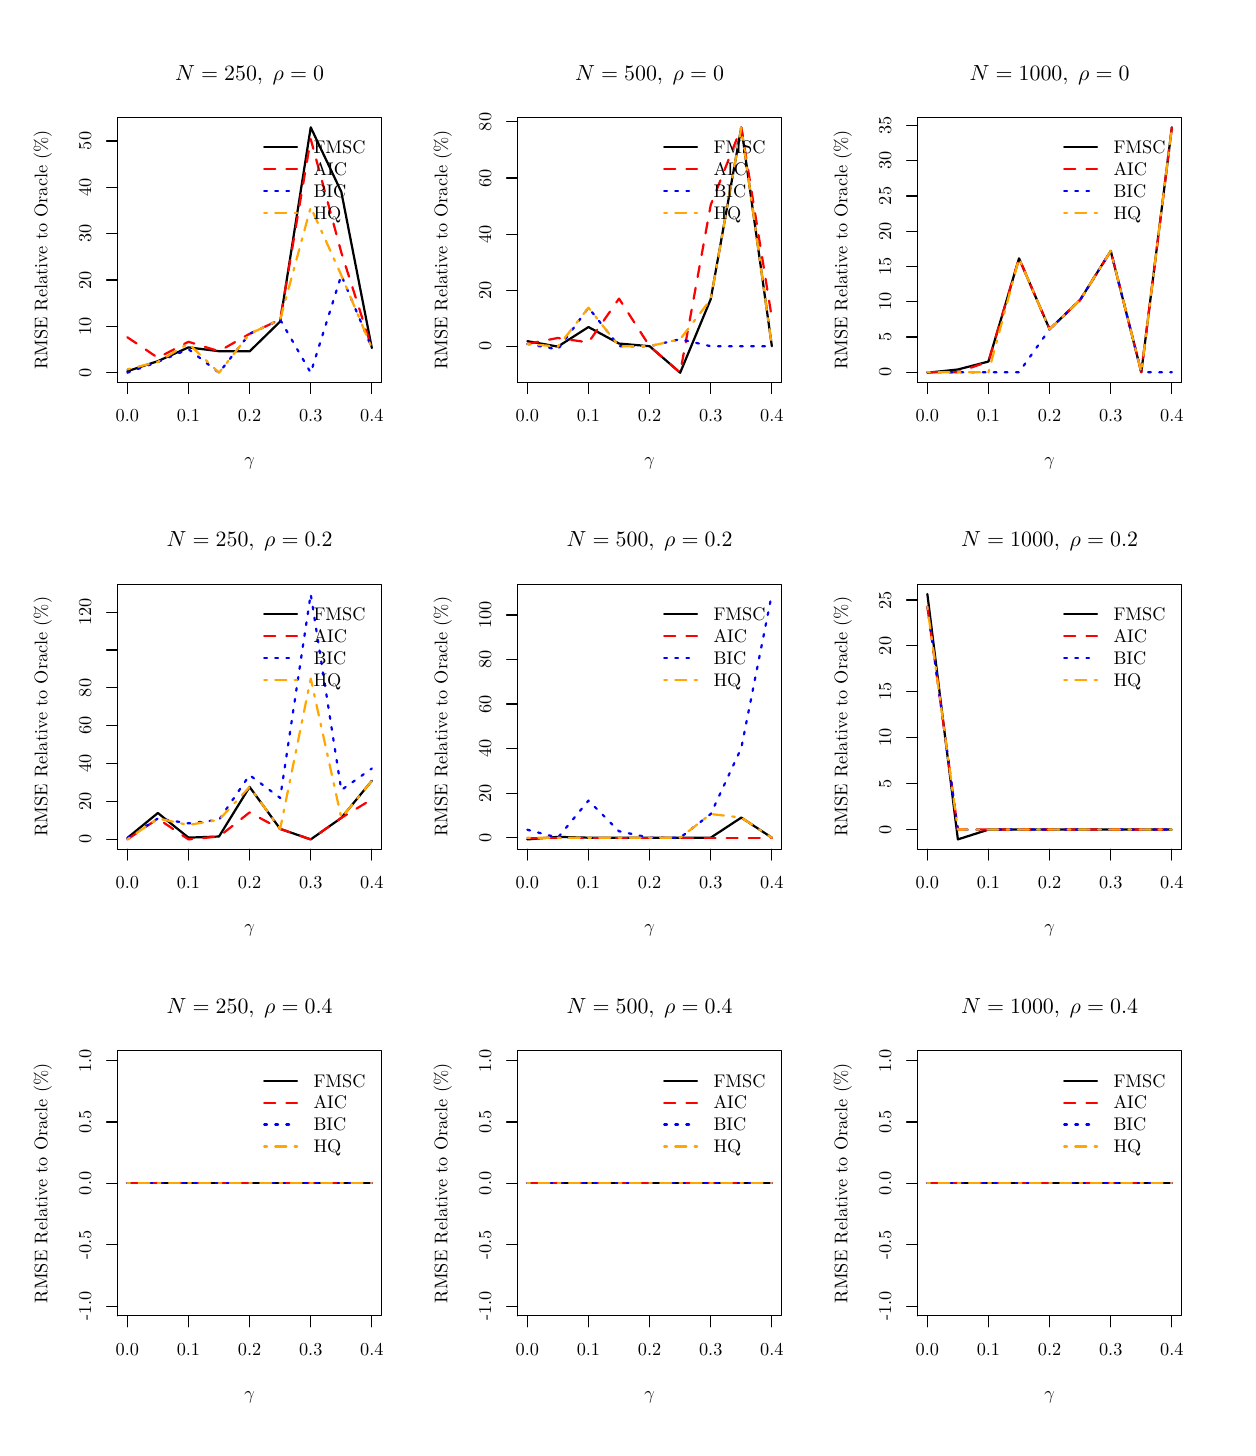
\begin{tikzpicture}[x=1pt,y=1pt]
\definecolor[named]{fillColor}{rgb}{1.00,1.00,1.00}
\path[use as bounding box,fill=fillColor,fill opacity=0.00] (0,0) rectangle (433.62,505.89);
\begin{scope}
\path[clip] ( 32.47,377.65) rectangle (127.91,473.42);
\definecolor[named]{drawColor}{rgb}{0.00,0.00,0.00}

\path[draw=drawColor,line width= 0.8pt,line join=round,line cap=round] ( 36.01,381.73) --
	( 47.05,385.39) --
	( 58.10,390.36) --
	( 69.14,388.97) --
	( 80.19,388.92) --
	( 91.24,399.70) --
	(102.28,469.87) --
	(113.33,446.56) --
	(124.37,390.09);
\end{scope}
\begin{scope}
\path[clip] (  0.00,  0.00) rectangle (433.62,505.89);
\definecolor[named]{drawColor}{rgb}{0.00,0.00,0.00}

\path[draw=drawColor,line width= 0.4pt,line join=round,line cap=round] ( 36.01,377.65) -- (124.37,377.65);

\path[draw=drawColor,line width= 0.4pt,line join=round,line cap=round] ( 36.01,377.65) -- ( 36.01,373.69);

\path[draw=drawColor,line width= 0.4pt,line join=round,line cap=round] ( 58.10,377.65) -- ( 58.10,373.69);

\path[draw=drawColor,line width= 0.4pt,line join=round,line cap=round] ( 80.19,377.65) -- ( 80.19,373.69);

\path[draw=drawColor,line width= 0.4pt,line join=round,line cap=round] (102.28,377.65) -- (102.28,373.69);

\path[draw=drawColor,line width= 0.4pt,line join=round,line cap=round] (124.37,377.65) -- (124.37,373.69);

\node[text=drawColor,anchor=base,inner sep=0pt, outer sep=0pt, scale=  0.66] at ( 36.01,363.40) {0.0};

\node[text=drawColor,anchor=base,inner sep=0pt, outer sep=0pt, scale=  0.66] at ( 58.10,363.40) {0.1};

\node[text=drawColor,anchor=base,inner sep=0pt, outer sep=0pt, scale=  0.66] at ( 80.19,363.40) {0.2};

\node[text=drawColor,anchor=base,inner sep=0pt, outer sep=0pt, scale=  0.66] at (102.28,363.40) {0.3};

\node[text=drawColor,anchor=base,inner sep=0pt, outer sep=0pt, scale=  0.66] at (124.37,363.40) {0.4};

\path[draw=drawColor,line width= 0.4pt,line join=round,line cap=round] ( 32.47,381.20) -- ( 32.47,464.94);

\path[draw=drawColor,line width= 0.4pt,line join=round,line cap=round] ( 32.47,381.20) -- ( 28.51,381.20);

\path[draw=drawColor,line width= 0.4pt,line join=round,line cap=round] ( 32.47,397.95) -- ( 28.51,397.95);

\path[draw=drawColor,line width= 0.4pt,line join=round,line cap=round] ( 32.47,414.70) -- ( 28.51,414.70);

\path[draw=drawColor,line width= 0.4pt,line join=round,line cap=round] ( 32.47,431.44) -- ( 28.51,431.44);

\path[draw=drawColor,line width= 0.4pt,line join=round,line cap=round] ( 32.47,448.19) -- ( 28.51,448.19);

\path[draw=drawColor,line width= 0.4pt,line join=round,line cap=round] ( 32.47,464.94) -- ( 28.51,464.94);

\node[text=drawColor,rotate= 90.00,anchor=base,inner sep=0pt, outer sep=0pt, scale=  0.66] at ( 22.97,381.20) {0};

\node[text=drawColor,rotate= 90.00,anchor=base,inner sep=0pt, outer sep=0pt, scale=  0.66] at ( 22.97,397.95) {10};

\node[text=drawColor,rotate= 90.00,anchor=base,inner sep=0pt, outer sep=0pt, scale=  0.66] at ( 22.97,414.70) {20};

\node[text=drawColor,rotate= 90.00,anchor=base,inner sep=0pt, outer sep=0pt, scale=  0.66] at ( 22.97,431.44) {30};

\node[text=drawColor,rotate= 90.00,anchor=base,inner sep=0pt, outer sep=0pt, scale=  0.66] at ( 22.97,448.19) {40};

\node[text=drawColor,rotate= 90.00,anchor=base,inner sep=0pt, outer sep=0pt, scale=  0.66] at ( 22.97,464.94) {50};

\path[draw=drawColor,line width= 0.4pt,line join=round,line cap=round] ( 32.47,377.65) --
	(127.91,377.65) --
	(127.91,473.42) --
	( 32.47,473.42) --
	( 32.47,377.65);
\end{scope}
\begin{scope}
\path[clip] (  0.00,337.26) rectangle (144.54,505.89);
\definecolor[named]{drawColor}{rgb}{0.00,0.00,0.00}

\node[text=drawColor,anchor=base,inner sep=0pt, outer sep=0pt, scale=  0.79] at ( 80.19,486.92) {\bfseries $N=250, \;\rho=0$};

\node[text=drawColor,anchor=base,inner sep=0pt, outer sep=0pt, scale=  0.66] at ( 80.19,347.56) {$\gamma$};

\node[text=drawColor,rotate= 90.00,anchor=base,inner sep=0pt, outer sep=0pt, scale=  0.66] at (  7.13,425.53) {RMSE Relative to Oracle (\%)};
\end{scope}
\begin{scope}
\path[clip] ( 32.47,377.65) rectangle (127.91,473.42);
\definecolor[named]{drawColor}{rgb}{1.00,0.00,0.00}

\path[draw=drawColor,line width= 0.8pt,dash pattern=on 4pt off 4pt ,line join=round,line cap=round] ( 36.01,394.03) --
	( 47.05,386.59) --
	( 58.10,392.38) --
	( 69.14,388.97) --
	( 80.19,395.26) --
	( 91.24,400.39) --
	(102.28,465.62) --
	(113.33,424.66) --
	(124.37,390.09);
\definecolor[named]{drawColor}{rgb}{0.00,0.00,1.00}

\path[draw=drawColor,line width= 0.8pt,dash pattern=on 1pt off 3pt ,line join=round,line cap=round] ( 36.01,381.20) --
	( 47.05,385.12) --
	( 58.10,389.72) --
	( 69.14,381.20) --
	( 80.19,395.26) --
	( 91.24,400.39) --
	(102.28,381.20) --
	(113.33,416.43) --
	(124.37,390.09);
\definecolor[named]{drawColor}{rgb}{1.00,0.65,0.00}

\path[draw=drawColor,line width= 0.8pt,dash pattern=on 1pt off 3pt on 4pt off 3pt ,line join=round,line cap=round] ( 36.01,382.42) --
	( 47.05,385.12) --
	( 58.10,391.75) --
	( 69.14,381.20) --
	( 80.19,395.26) --
	( 91.24,400.39) --
	(102.28,441.04) --
	(113.33,416.43) --
	(124.37,390.09);
\definecolor[named]{drawColor}{rgb}{0.00,0.00,0.00}

\path[draw=drawColor,line width= 0.8pt,line join=round,line cap=round] ( 85.47,462.63) -- ( 97.35,462.63);
\definecolor[named]{drawColor}{rgb}{1.00,0.00,0.00}

\path[draw=drawColor,line width= 0.8pt,dash pattern=on 4pt off 4pt ,line join=round,line cap=round] ( 85.47,454.71) -- ( 97.35,454.71);
\definecolor[named]{drawColor}{rgb}{0.00,0.00,1.00}

\path[draw=drawColor,line width= 0.8pt,dash pattern=on 1pt off 3pt ,line join=round,line cap=round] ( 85.47,446.79) -- ( 97.35,446.79);
\definecolor[named]{drawColor}{rgb}{1.00,0.65,0.00}

\path[draw=drawColor,line width= 0.8pt,dash pattern=on 1pt off 3pt on 4pt off 3pt ,line join=round,line cap=round] ( 85.47,438.87) -- ( 97.35,438.87);
\definecolor[named]{drawColor}{rgb}{0.00,0.00,0.00}

\node[text=drawColor,anchor=base west,inner sep=0pt, outer sep=0pt, scale=  0.66] at (103.29,460.35) {FMSC};

\node[text=drawColor,anchor=base west,inner sep=0pt, outer sep=0pt, scale=  0.66] at (103.29,452.43) {AIC};

\node[text=drawColor,anchor=base west,inner sep=0pt, outer sep=0pt, scale=  0.66] at (103.29,444.51) {BIC};

\node[text=drawColor,anchor=base west,inner sep=0pt, outer sep=0pt, scale=  0.66] at (103.29,436.59) {HQ};
\end{scope}
\begin{scope}
\path[clip] (177.01,377.65) rectangle (272.45,473.42);
\definecolor[named]{drawColor}{rgb}{0.00,0.00,0.00}

\path[draw=drawColor,line width= 0.8pt,line join=round,line cap=round] (180.55,392.61) --
	(191.59,390.64) --
	(202.64,397.71) --
	(213.68,391.74) --
	(224.73,390.78) --
	(235.78,381.20) --
	(246.82,407.78) --
	(257.87,469.87) --
	(268.91,390.78);
\end{scope}
\begin{scope}
\path[clip] (  0.00,  0.00) rectangle (433.62,505.89);
\definecolor[named]{drawColor}{rgb}{0.00,0.00,0.00}

\path[draw=drawColor,line width= 0.4pt,line join=round,line cap=round] (180.55,377.65) -- (268.91,377.65);

\path[draw=drawColor,line width= 0.4pt,line join=round,line cap=round] (180.55,377.65) -- (180.55,373.69);

\path[draw=drawColor,line width= 0.4pt,line join=round,line cap=round] (202.64,377.65) -- (202.64,373.69);

\path[draw=drawColor,line width= 0.4pt,line join=round,line cap=round] (224.73,377.65) -- (224.73,373.69);

\path[draw=drawColor,line width= 0.4pt,line join=round,line cap=round] (246.82,377.65) -- (246.82,373.69);

\path[draw=drawColor,line width= 0.4pt,line join=round,line cap=round] (268.91,377.65) -- (268.91,373.69);

\node[text=drawColor,anchor=base,inner sep=0pt, outer sep=0pt, scale=  0.66] at (180.55,363.40) {0.0};

\node[text=drawColor,anchor=base,inner sep=0pt, outer sep=0pt, scale=  0.66] at (202.64,363.40) {0.1};

\node[text=drawColor,anchor=base,inner sep=0pt, outer sep=0pt, scale=  0.66] at (224.73,363.40) {0.2};

\node[text=drawColor,anchor=base,inner sep=0pt, outer sep=0pt, scale=  0.66] at (246.82,363.40) {0.3};

\node[text=drawColor,anchor=base,inner sep=0pt, outer sep=0pt, scale=  0.66] at (268.91,363.40) {0.4};

\path[draw=drawColor,line width= 0.4pt,line join=round,line cap=round] (177.01,390.78) -- (177.01,471.82);

\path[draw=drawColor,line width= 0.4pt,line join=round,line cap=round] (177.01,390.78) -- (173.05,390.78);

\path[draw=drawColor,line width= 0.4pt,line join=round,line cap=round] (177.01,411.04) -- (173.05,411.04);

\path[draw=drawColor,line width= 0.4pt,line join=round,line cap=round] (177.01,431.30) -- (173.05,431.30);

\path[draw=drawColor,line width= 0.4pt,line join=round,line cap=round] (177.01,451.56) -- (173.05,451.56);

\path[draw=drawColor,line width= 0.4pt,line join=round,line cap=round] (177.01,471.82) -- (173.05,471.82);

\node[text=drawColor,rotate= 90.00,anchor=base,inner sep=0pt, outer sep=0pt, scale=  0.66] at (167.51,390.78) {0};

\node[text=drawColor,rotate= 90.00,anchor=base,inner sep=0pt, outer sep=0pt, scale=  0.66] at (167.51,411.04) {20};

\node[text=drawColor,rotate= 90.00,anchor=base,inner sep=0pt, outer sep=0pt, scale=  0.66] at (167.51,431.30) {40};

\node[text=drawColor,rotate= 90.00,anchor=base,inner sep=0pt, outer sep=0pt, scale=  0.66] at (167.51,451.56) {60};

\node[text=drawColor,rotate= 90.00,anchor=base,inner sep=0pt, outer sep=0pt, scale=  0.66] at (167.51,471.82) {80};

\path[draw=drawColor,line width= 0.4pt,line join=round,line cap=round] (177.01,377.65) --
	(272.45,377.65) --
	(272.45,473.42) --
	(177.01,473.42) --
	(177.01,377.65);
\end{scope}
\begin{scope}
\path[clip] (144.54,337.26) rectangle (289.08,505.89);
\definecolor[named]{drawColor}{rgb}{0.00,0.00,0.00}

\node[text=drawColor,anchor=base,inner sep=0pt, outer sep=0pt, scale=  0.79] at (224.73,486.92) {\bfseries $N=500, \;\rho=0$};

\node[text=drawColor,anchor=base,inner sep=0pt, outer sep=0pt, scale=  0.66] at (224.73,347.56) {$\gamma$};

\node[text=drawColor,rotate= 90.00,anchor=base,inner sep=0pt, outer sep=0pt, scale=  0.66] at (151.67,425.53) {RMSE Relative to Oracle (\%)};
\end{scope}
\begin{scope}
\path[clip] (177.01,377.65) rectangle (272.45,473.42);
\definecolor[named]{drawColor}{rgb}{1.00,0.00,0.00}

\path[draw=drawColor,line width= 0.8pt,dash pattern=on 4pt off 4pt ,line join=round,line cap=round] (180.55,391.61) --
	(191.59,393.77) --
	(202.64,392.14) --
	(213.68,407.99) --
	(224.73,390.78) --
	(235.78,381.20) --
	(246.82,441.84) --
	(257.87,469.87) --
	(268.91,400.98);
\definecolor[named]{drawColor}{rgb}{0.00,0.00,1.00}

\path[draw=drawColor,line width= 0.8pt,dash pattern=on 1pt off 3pt ,line join=round,line cap=round] (180.55,391.61) --
	(191.59,389.62) --
	(202.64,404.71) --
	(213.68,390.78) --
	(224.73,390.78) --
	(235.78,393.31) --
	(246.82,390.78) --
	(257.87,390.78) --
	(268.91,390.78);
\definecolor[named]{drawColor}{rgb}{1.00,0.65,0.00}

\path[draw=drawColor,line width= 0.8pt,dash pattern=on 1pt off 3pt on 4pt off 3pt ,line join=round,line cap=round] (180.55,391.61) --
	(191.59,390.64) --
	(202.64,404.71) --
	(213.68,390.78) --
	(224.73,390.78) --
	(235.78,393.31) --
	(246.82,407.71) --
	(257.87,469.87) --
	(268.91,390.78);
\definecolor[named]{drawColor}{rgb}{0.00,0.00,0.00}

\path[draw=drawColor,line width= 0.8pt,line join=round,line cap=round] (230.01,462.63) -- (241.89,462.63);
\definecolor[named]{drawColor}{rgb}{1.00,0.00,0.00}

\path[draw=drawColor,line width= 0.8pt,dash pattern=on 4pt off 4pt ,line join=round,line cap=round] (230.01,454.71) -- (241.89,454.71);
\definecolor[named]{drawColor}{rgb}{0.00,0.00,1.00}

\path[draw=drawColor,line width= 0.8pt,dash pattern=on 1pt off 3pt ,line join=round,line cap=round] (230.01,446.79) -- (241.89,446.79);
\definecolor[named]{drawColor}{rgb}{1.00,0.65,0.00}

\path[draw=drawColor,line width= 0.8pt,dash pattern=on 1pt off 3pt on 4pt off 3pt ,line join=round,line cap=round] (230.01,438.87) -- (241.89,438.87);
\definecolor[named]{drawColor}{rgb}{0.00,0.00,0.00}

\node[text=drawColor,anchor=base west,inner sep=0pt, outer sep=0pt, scale=  0.66] at (247.83,460.35) {FMSC};

\node[text=drawColor,anchor=base west,inner sep=0pt, outer sep=0pt, scale=  0.66] at (247.83,452.43) {AIC};

\node[text=drawColor,anchor=base west,inner sep=0pt, outer sep=0pt, scale=  0.66] at (247.83,444.51) {BIC};

\node[text=drawColor,anchor=base west,inner sep=0pt, outer sep=0pt, scale=  0.66] at (247.83,436.59) {HQ};
\end{scope}
\begin{scope}
\path[clip] (321.55,377.65) rectangle (416.99,473.42);
\definecolor[named]{drawColor}{rgb}{0.00,0.00,0.00}

\path[draw=drawColor,line width= 0.8pt,line join=round,line cap=round] (325.09,381.20) --
	(336.13,382.37) --
	(347.18,385.24) --
	(358.22,422.53) --
	(369.27,396.91) --
	(380.32,407.55) --
	(391.36,425.20) --
	(402.41,381.38) --
	(413.45,469.87);
\end{scope}
\begin{scope}
\path[clip] (  0.00,  0.00) rectangle (433.62,505.89);
\definecolor[named]{drawColor}{rgb}{0.00,0.00,0.00}

\path[draw=drawColor,line width= 0.4pt,line join=round,line cap=round] (325.09,377.65) -- (413.45,377.65);

\path[draw=drawColor,line width= 0.4pt,line join=round,line cap=round] (325.09,377.65) -- (325.09,373.69);

\path[draw=drawColor,line width= 0.4pt,line join=round,line cap=round] (347.18,377.65) -- (347.18,373.69);

\path[draw=drawColor,line width= 0.4pt,line join=round,line cap=round] (369.27,377.65) -- (369.27,373.69);

\path[draw=drawColor,line width= 0.4pt,line join=round,line cap=round] (391.36,377.65) -- (391.36,373.69);

\path[draw=drawColor,line width= 0.4pt,line join=round,line cap=round] (413.45,377.65) -- (413.45,373.69);

\node[text=drawColor,anchor=base,inner sep=0pt, outer sep=0pt, scale=  0.66] at (325.09,363.40) {0.0};

\node[text=drawColor,anchor=base,inner sep=0pt, outer sep=0pt, scale=  0.66] at (347.18,363.40) {0.1};

\node[text=drawColor,anchor=base,inner sep=0pt, outer sep=0pt, scale=  0.66] at (369.27,363.40) {0.2};

\node[text=drawColor,anchor=base,inner sep=0pt, outer sep=0pt, scale=  0.66] at (391.36,363.40) {0.3};

\node[text=drawColor,anchor=base,inner sep=0pt, outer sep=0pt, scale=  0.66] at (413.45,363.40) {0.4};

\path[draw=drawColor,line width= 0.4pt,line join=round,line cap=round] (321.55,381.38) -- (321.55,470.55);

\path[draw=drawColor,line width= 0.4pt,line join=round,line cap=round] (321.55,381.38) -- (317.59,381.38);

\path[draw=drawColor,line width= 0.4pt,line join=round,line cap=round] (321.55,394.12) -- (317.59,394.12);

\path[draw=drawColor,line width= 0.4pt,line join=round,line cap=round] (321.55,406.86) -- (317.59,406.86);

\path[draw=drawColor,line width= 0.4pt,line join=round,line cap=round] (321.55,419.60) -- (317.59,419.60);

\path[draw=drawColor,line width= 0.4pt,line join=round,line cap=round] (321.55,432.34) -- (317.59,432.34);

\path[draw=drawColor,line width= 0.4pt,line join=round,line cap=round] (321.55,445.07) -- (317.59,445.07);

\path[draw=drawColor,line width= 0.4pt,line join=round,line cap=round] (321.55,457.81) -- (317.59,457.81);

\path[draw=drawColor,line width= 0.4pt,line join=round,line cap=round] (321.55,470.55) -- (317.59,470.55);

\node[text=drawColor,rotate= 90.00,anchor=base,inner sep=0pt, outer sep=0pt, scale=  0.66] at (312.05,381.38) {0};

\node[text=drawColor,rotate= 90.00,anchor=base,inner sep=0pt, outer sep=0pt, scale=  0.66] at (312.05,394.12) {5};

\node[text=drawColor,rotate= 90.00,anchor=base,inner sep=0pt, outer sep=0pt, scale=  0.66] at (312.05,406.86) {10};

\node[text=drawColor,rotate= 90.00,anchor=base,inner sep=0pt, outer sep=0pt, scale=  0.66] at (312.05,419.60) {15};

\node[text=drawColor,rotate= 90.00,anchor=base,inner sep=0pt, outer sep=0pt, scale=  0.66] at (312.05,432.34) {20};

\node[text=drawColor,rotate= 90.00,anchor=base,inner sep=0pt, outer sep=0pt, scale=  0.66] at (312.05,445.07) {25};

\node[text=drawColor,rotate= 90.00,anchor=base,inner sep=0pt, outer sep=0pt, scale=  0.66] at (312.05,457.81) {30};

\node[text=drawColor,rotate= 90.00,anchor=base,inner sep=0pt, outer sep=0pt, scale=  0.66] at (312.05,470.55) {35};

\path[draw=drawColor,line width= 0.4pt,line join=round,line cap=round] (321.55,377.65) --
	(416.99,377.65) --
	(416.99,473.42) --
	(321.55,473.42) --
	(321.55,377.65);
\end{scope}
\begin{scope}
\path[clip] (289.08,337.26) rectangle (433.62,505.89);
\definecolor[named]{drawColor}{rgb}{0.00,0.00,0.00}

\node[text=drawColor,anchor=base,inner sep=0pt, outer sep=0pt, scale=  0.79] at (369.27,486.92) {\bfseries $N=1000, \;\rho=0$};

\node[text=drawColor,anchor=base,inner sep=0pt, outer sep=0pt, scale=  0.66] at (369.27,347.56) {$\gamma$};

\node[text=drawColor,rotate= 90.00,anchor=base,inner sep=0pt, outer sep=0pt, scale=  0.66] at (296.21,425.53) {RMSE Relative to Oracle (\%)};
\end{scope}
\begin{scope}
\path[clip] (321.55,377.65) rectangle (416.99,473.42);
\definecolor[named]{drawColor}{rgb}{1.00,0.00,0.00}

\path[draw=drawColor,line width= 0.8pt,dash pattern=on 4pt off 4pt ,line join=round,line cap=round] (325.09,381.38) --
	(336.13,381.38) --
	(347.18,385.24) --
	(358.22,422.53) --
	(369.27,396.91) --
	(380.32,407.55) --
	(391.36,425.20) --
	(402.41,381.38) --
	(413.45,469.87);
\definecolor[named]{drawColor}{rgb}{0.00,0.00,1.00}

\path[draw=drawColor,line width= 0.8pt,dash pattern=on 1pt off 3pt ,line join=round,line cap=round] (325.09,381.38) --
	(336.13,381.38) --
	(347.18,381.38) --
	(358.22,381.38) --
	(369.27,396.91) --
	(380.32,407.55) --
	(391.36,425.20) --
	(402.41,381.38) --
	(413.45,381.38);
\definecolor[named]{drawColor}{rgb}{1.00,0.65,0.00}

\path[draw=drawColor,line width= 0.8pt,dash pattern=on 1pt off 3pt on 4pt off 3pt ,line join=round,line cap=round] (325.09,381.38) --
	(336.13,381.38) --
	(347.18,381.38) --
	(358.22,422.53) --
	(369.27,396.91) --
	(380.32,407.55) --
	(391.36,425.20) --
	(402.41,381.38) --
	(413.45,469.87);
\definecolor[named]{drawColor}{rgb}{0.00,0.00,0.00}

\path[draw=drawColor,line width= 0.8pt,line join=round,line cap=round] (374.55,462.63) -- (386.43,462.63);
\definecolor[named]{drawColor}{rgb}{1.00,0.00,0.00}

\path[draw=drawColor,line width= 0.8pt,dash pattern=on 4pt off 4pt ,line join=round,line cap=round] (374.55,454.71) -- (386.43,454.71);
\definecolor[named]{drawColor}{rgb}{0.00,0.00,1.00}

\path[draw=drawColor,line width= 0.8pt,dash pattern=on 1pt off 3pt ,line join=round,line cap=round] (374.55,446.79) -- (386.43,446.79);
\definecolor[named]{drawColor}{rgb}{1.00,0.65,0.00}

\path[draw=drawColor,line width= 0.8pt,dash pattern=on 1pt off 3pt on 4pt off 3pt ,line join=round,line cap=round] (374.55,438.87) -- (386.43,438.87);
\definecolor[named]{drawColor}{rgb}{0.00,0.00,0.00}

\node[text=drawColor,anchor=base west,inner sep=0pt, outer sep=0pt, scale=  0.66] at (392.37,460.35) {FMSC};

\node[text=drawColor,anchor=base west,inner sep=0pt, outer sep=0pt, scale=  0.66] at (392.37,452.43) {AIC};

\node[text=drawColor,anchor=base west,inner sep=0pt, outer sep=0pt, scale=  0.66] at (392.37,444.51) {BIC};

\node[text=drawColor,anchor=base west,inner sep=0pt, outer sep=0pt, scale=  0.66] at (392.37,436.59) {HQ};
\end{scope}
\begin{scope}
\path[clip] ( 32.47,209.02) rectangle (127.91,304.79);
\definecolor[named]{drawColor}{rgb}{0.00,0.00,0.00}

\path[draw=drawColor,line width= 0.8pt,line join=round,line cap=round] ( 36.01,213.08) --
	( 47.05,222.11) --
	( 58.10,213.21) --
	( 69.14,213.61) --
	( 80.19,231.53) --
	( 91.24,216.36) --
	(102.28,212.57) --
	(113.33,220.34) --
	(124.37,233.76);
\end{scope}
\begin{scope}
\path[clip] (  0.00,  0.00) rectangle (433.62,505.89);
\definecolor[named]{drawColor}{rgb}{0.00,0.00,0.00}

\path[draw=drawColor,line width= 0.4pt,line join=round,line cap=round] ( 36.01,209.02) -- (124.37,209.02);

\path[draw=drawColor,line width= 0.4pt,line join=round,line cap=round] ( 36.01,209.02) -- ( 36.01,205.06);

\path[draw=drawColor,line width= 0.4pt,line join=round,line cap=round] ( 58.10,209.02) -- ( 58.10,205.06);

\path[draw=drawColor,line width= 0.4pt,line join=round,line cap=round] ( 80.19,209.02) -- ( 80.19,205.06);

\path[draw=drawColor,line width= 0.4pt,line join=round,line cap=round] (102.28,209.02) -- (102.28,205.06);

\path[draw=drawColor,line width= 0.4pt,line join=round,line cap=round] (124.37,209.02) -- (124.37,205.06);

\node[text=drawColor,anchor=base,inner sep=0pt, outer sep=0pt, scale=  0.66] at ( 36.01,194.77) {0.0};

\node[text=drawColor,anchor=base,inner sep=0pt, outer sep=0pt, scale=  0.66] at ( 58.10,194.77) {0.1};

\node[text=drawColor,anchor=base,inner sep=0pt, outer sep=0pt, scale=  0.66] at ( 80.19,194.77) {0.2};

\node[text=drawColor,anchor=base,inner sep=0pt, outer sep=0pt, scale=  0.66] at (102.28,194.77) {0.3};

\node[text=drawColor,anchor=base,inner sep=0pt, outer sep=0pt, scale=  0.66] at (124.37,194.77) {0.4};

\path[draw=drawColor,line width= 0.4pt,line join=round,line cap=round] ( 32.47,212.57) -- ( 32.47,294.68);

\path[draw=drawColor,line width= 0.4pt,line join=round,line cap=round] ( 32.47,212.57) -- ( 28.51,212.57);

\path[draw=drawColor,line width= 0.4pt,line join=round,line cap=round] ( 32.47,226.25) -- ( 28.51,226.25);

\path[draw=drawColor,line width= 0.4pt,line join=round,line cap=round] ( 32.47,239.94) -- ( 28.51,239.94);

\path[draw=drawColor,line width= 0.4pt,line join=round,line cap=round] ( 32.47,253.62) -- ( 28.51,253.62);

\path[draw=drawColor,line width= 0.4pt,line join=round,line cap=round] ( 32.47,267.31) -- ( 28.51,267.31);

\path[draw=drawColor,line width= 0.4pt,line join=round,line cap=round] ( 32.47,280.99) -- ( 28.51,280.99);

\path[draw=drawColor,line width= 0.4pt,line join=round,line cap=round] ( 32.47,294.68) -- ( 28.51,294.68);

\node[text=drawColor,rotate= 90.00,anchor=base,inner sep=0pt, outer sep=0pt, scale=  0.66] at ( 22.97,212.57) {0};

\node[text=drawColor,rotate= 90.00,anchor=base,inner sep=0pt, outer sep=0pt, scale=  0.66] at ( 22.97,226.25) {20};

\node[text=drawColor,rotate= 90.00,anchor=base,inner sep=0pt, outer sep=0pt, scale=  0.66] at ( 22.97,239.94) {40};

\node[text=drawColor,rotate= 90.00,anchor=base,inner sep=0pt, outer sep=0pt, scale=  0.66] at ( 22.97,253.62) {60};

\node[text=drawColor,rotate= 90.00,anchor=base,inner sep=0pt, outer sep=0pt, scale=  0.66] at ( 22.97,267.31) {80};

\node[text=drawColor,rotate= 90.00,anchor=base,inner sep=0pt, outer sep=0pt, scale=  0.66] at ( 22.97,294.68) {120};

\path[draw=drawColor,line width= 0.4pt,line join=round,line cap=round] ( 32.47,209.02) --
	(127.91,209.02) --
	(127.91,304.79) --
	( 32.47,304.79) --
	( 32.47,209.02);
\end{scope}
\begin{scope}
\path[clip] (  0.00,168.63) rectangle (144.54,337.26);
\definecolor[named]{drawColor}{rgb}{0.00,0.00,0.00}

\node[text=drawColor,anchor=base,inner sep=0pt, outer sep=0pt, scale=  0.79] at ( 80.19,318.29) {\bfseries $N=250, \;\rho=0.2$};

\node[text=drawColor,anchor=base,inner sep=0pt, outer sep=0pt, scale=  0.66] at ( 80.19,178.93) {$\gamma$};

\node[text=drawColor,rotate= 90.00,anchor=base,inner sep=0pt, outer sep=0pt, scale=  0.66] at (  7.13,256.90) {RMSE Relative to Oracle (\%)};
\end{scope}
\begin{scope}
\path[clip] ( 32.47,209.02) rectangle (127.91,304.79);
\definecolor[named]{drawColor}{rgb}{1.00,0.00,0.00}

\path[draw=drawColor,line width= 0.8pt,dash pattern=on 4pt off 4pt ,line join=round,line cap=round] ( 36.01,212.57) --
	( 47.05,220.05) --
	( 58.10,212.57) --
	( 69.14,213.61) --
	( 80.19,222.32) --
	( 91.24,216.36) --
	(102.28,212.57) --
	(113.33,220.34) --
	(124.37,227.06);
\definecolor[named]{drawColor}{rgb}{0.00,0.00,1.00}

\path[draw=drawColor,line width= 0.8pt,dash pattern=on 1pt off 3pt ,line join=round,line cap=round] ( 36.01,213.00) --
	( 47.05,220.14) --
	( 58.10,218.37) --
	( 69.14,219.64) --
	( 80.19,235.81) --
	( 91.24,227.55) --
	(102.28,301.24) --
	(113.33,230.38) --
	(124.37,238.20);
\definecolor[named]{drawColor}{rgb}{1.00,0.65,0.00}

\path[draw=drawColor,line width= 0.8pt,dash pattern=on 1pt off 3pt on 4pt off 3pt ,line join=round,line cap=round] ( 36.01,212.57) --
	( 47.05,220.14) --
	( 58.10,217.78) --
	( 69.14,219.64) --
	( 80.19,231.53) --
	( 91.24,216.36) --
	(102.28,270.68) --
	(113.33,220.34) --
	(124.37,233.76);
\definecolor[named]{drawColor}{rgb}{0.00,0.00,0.00}

\path[draw=drawColor,line width= 0.8pt,line join=round,line cap=round] ( 85.47,294.00) -- ( 97.35,294.00);
\definecolor[named]{drawColor}{rgb}{1.00,0.00,0.00}

\path[draw=drawColor,line width= 0.8pt,dash pattern=on 4pt off 4pt ,line join=round,line cap=round] ( 85.47,286.08) -- ( 97.35,286.08);
\definecolor[named]{drawColor}{rgb}{0.00,0.00,1.00}

\path[draw=drawColor,line width= 0.8pt,dash pattern=on 1pt off 3pt ,line join=round,line cap=round] ( 85.47,278.16) -- ( 97.35,278.16);
\definecolor[named]{drawColor}{rgb}{1.00,0.65,0.00}

\path[draw=drawColor,line width= 0.8pt,dash pattern=on 1pt off 3pt on 4pt off 3pt ,line join=round,line cap=round] ( 85.47,270.24) -- ( 97.35,270.24);
\definecolor[named]{drawColor}{rgb}{0.00,0.00,0.00}

\node[text=drawColor,anchor=base west,inner sep=0pt, outer sep=0pt, scale=  0.66] at (103.29,291.72) {FMSC};

\node[text=drawColor,anchor=base west,inner sep=0pt, outer sep=0pt, scale=  0.66] at (103.29,283.80) {AIC};

\node[text=drawColor,anchor=base west,inner sep=0pt, outer sep=0pt, scale=  0.66] at (103.29,275.88) {BIC};

\node[text=drawColor,anchor=base west,inner sep=0pt, outer sep=0pt, scale=  0.66] at (103.29,267.96) {HQ};
\end{scope}
\begin{scope}
\path[clip] (177.01,209.02) rectangle (272.45,304.79);
\definecolor[named]{drawColor}{rgb}{0.00,0.00,0.00}

\path[draw=drawColor,line width= 0.8pt,line join=round,line cap=round] (180.55,212.57) --
	(191.59,213.47) --
	(202.64,213.19) --
	(213.68,213.19) --
	(224.73,213.19) --
	(235.78,213.19) --
	(246.82,213.19) --
	(257.87,220.45) --
	(268.91,213.19);
\end{scope}
\begin{scope}
\path[clip] (  0.00,  0.00) rectangle (433.62,505.89);
\definecolor[named]{drawColor}{rgb}{0.00,0.00,0.00}

\path[draw=drawColor,line width= 0.4pt,line join=round,line cap=round] (180.55,209.02) -- (268.91,209.02);

\path[draw=drawColor,line width= 0.4pt,line join=round,line cap=round] (180.55,209.02) -- (180.55,205.06);

\path[draw=drawColor,line width= 0.4pt,line join=round,line cap=round] (202.64,209.02) -- (202.64,205.06);

\path[draw=drawColor,line width= 0.4pt,line join=round,line cap=round] (224.73,209.02) -- (224.73,205.06);

\path[draw=drawColor,line width= 0.4pt,line join=round,line cap=round] (246.82,209.02) -- (246.82,205.06);

\path[draw=drawColor,line width= 0.4pt,line join=round,line cap=round] (268.91,209.02) -- (268.91,205.06);

\node[text=drawColor,anchor=base,inner sep=0pt, outer sep=0pt, scale=  0.66] at (180.55,194.77) {0.0};

\node[text=drawColor,anchor=base,inner sep=0pt, outer sep=0pt, scale=  0.66] at (202.64,194.77) {0.1};

\node[text=drawColor,anchor=base,inner sep=0pt, outer sep=0pt, scale=  0.66] at (224.73,194.77) {0.2};

\node[text=drawColor,anchor=base,inner sep=0pt, outer sep=0pt, scale=  0.66] at (246.82,194.77) {0.3};

\node[text=drawColor,anchor=base,inner sep=0pt, outer sep=0pt, scale=  0.66] at (268.91,194.77) {0.4};

\path[draw=drawColor,line width= 0.4pt,line join=round,line cap=round] (177.01,213.19) -- (177.01,293.67);

\path[draw=drawColor,line width= 0.4pt,line join=round,line cap=round] (177.01,213.19) -- (173.05,213.19);

\path[draw=drawColor,line width= 0.4pt,line join=round,line cap=round] (177.01,229.29) -- (173.05,229.29);

\path[draw=drawColor,line width= 0.4pt,line join=round,line cap=round] (177.01,245.38) -- (173.05,245.38);

\path[draw=drawColor,line width= 0.4pt,line join=round,line cap=round] (177.01,261.48) -- (173.05,261.48);

\path[draw=drawColor,line width= 0.4pt,line join=round,line cap=round] (177.01,277.57) -- (173.05,277.57);

\path[draw=drawColor,line width= 0.4pt,line join=round,line cap=round] (177.01,293.67) -- (173.05,293.67);

\node[text=drawColor,rotate= 90.00,anchor=base,inner sep=0pt, outer sep=0pt, scale=  0.66] at (167.51,213.19) {0};

\node[text=drawColor,rotate= 90.00,anchor=base,inner sep=0pt, outer sep=0pt, scale=  0.66] at (167.51,229.29) {20};

\node[text=drawColor,rotate= 90.00,anchor=base,inner sep=0pt, outer sep=0pt, scale=  0.66] at (167.51,245.38) {40};

\node[text=drawColor,rotate= 90.00,anchor=base,inner sep=0pt, outer sep=0pt, scale=  0.66] at (167.51,261.48) {60};

\node[text=drawColor,rotate= 90.00,anchor=base,inner sep=0pt, outer sep=0pt, scale=  0.66] at (167.51,277.57) {80};

\node[text=drawColor,rotate= 90.00,anchor=base,inner sep=0pt, outer sep=0pt, scale=  0.66] at (167.51,293.67) {100};

\path[draw=drawColor,line width= 0.4pt,line join=round,line cap=round] (177.01,209.02) --
	(272.45,209.02) --
	(272.45,304.79) --
	(177.01,304.79) --
	(177.01,209.02);
\end{scope}
\begin{scope}
\path[clip] (144.54,168.63) rectangle (289.08,337.26);
\definecolor[named]{drawColor}{rgb}{0.00,0.00,0.00}

\node[text=drawColor,anchor=base,inner sep=0pt, outer sep=0pt, scale=  0.79] at (224.73,318.29) {\bfseries $N=500, \;\rho=0.2$};

\node[text=drawColor,anchor=base,inner sep=0pt, outer sep=0pt, scale=  0.66] at (224.73,178.93) {$\gamma$};

\node[text=drawColor,rotate= 90.00,anchor=base,inner sep=0pt, outer sep=0pt, scale=  0.66] at (151.67,256.90) {RMSE Relative to Oracle (\%)};
\end{scope}
\begin{scope}
\path[clip] (177.01,209.02) rectangle (272.45,304.79);
\definecolor[named]{drawColor}{rgb}{1.00,0.00,0.00}

\path[draw=drawColor,line width= 0.8pt,dash pattern=on 4pt off 4pt ,line join=round,line cap=round] (180.55,213.19) --
	(191.59,213.19) --
	(202.64,213.19) --
	(213.68,213.19) --
	(224.73,213.19) --
	(235.78,213.19) --
	(246.82,213.19) --
	(257.87,213.19) --
	(268.91,213.19);
\definecolor[named]{drawColor}{rgb}{0.00,0.00,1.00}

\path[draw=drawColor,line width= 0.8pt,dash pattern=on 1pt off 3pt ,line join=round,line cap=round] (180.55,216.06) --
	(191.59,213.19) --
	(202.64,226.59) --
	(213.68,215.52) --
	(224.73,213.19) --
	(235.78,213.19) --
	(246.82,221.75) --
	(257.87,245.61) --
	(268.91,301.24);
\definecolor[named]{drawColor}{rgb}{1.00,0.65,0.00}

\path[draw=drawColor,line width= 0.8pt,dash pattern=on 1pt off 3pt on 4pt off 3pt ,line join=round,line cap=round] (180.55,213.19) --
	(191.59,213.19) --
	(202.64,213.19) --
	(213.68,213.19) --
	(224.73,213.19) --
	(235.78,213.19) --
	(246.82,221.75) --
	(257.87,220.45) --
	(268.91,213.19);
\definecolor[named]{drawColor}{rgb}{0.00,0.00,0.00}

\path[draw=drawColor,line width= 0.8pt,line join=round,line cap=round] (230.01,294.00) -- (241.89,294.00);
\definecolor[named]{drawColor}{rgb}{1.00,0.00,0.00}

\path[draw=drawColor,line width= 0.8pt,dash pattern=on 4pt off 4pt ,line join=round,line cap=round] (230.01,286.08) -- (241.89,286.08);
\definecolor[named]{drawColor}{rgb}{0.00,0.00,1.00}

\path[draw=drawColor,line width= 0.8pt,dash pattern=on 1pt off 3pt ,line join=round,line cap=round] (230.01,278.16) -- (241.89,278.16);
\definecolor[named]{drawColor}{rgb}{1.00,0.65,0.00}

\path[draw=drawColor,line width= 0.8pt,dash pattern=on 1pt off 3pt on 4pt off 3pt ,line join=round,line cap=round] (230.01,270.24) -- (241.89,270.24);
\definecolor[named]{drawColor}{rgb}{0.00,0.00,0.00}

\node[text=drawColor,anchor=base west,inner sep=0pt, outer sep=0pt, scale=  0.66] at (247.83,291.72) {FMSC};

\node[text=drawColor,anchor=base west,inner sep=0pt, outer sep=0pt, scale=  0.66] at (247.83,283.80) {AIC};

\node[text=drawColor,anchor=base west,inner sep=0pt, outer sep=0pt, scale=  0.66] at (247.83,275.88) {BIC};

\node[text=drawColor,anchor=base west,inner sep=0pt, outer sep=0pt, scale=  0.66] at (247.83,267.96) {HQ};
\end{scope}
\begin{scope}
\path[clip] (321.55,209.02) rectangle (416.99,304.79);
\definecolor[named]{drawColor}{rgb}{0.00,0.00,0.00}

\path[draw=drawColor,line width= 0.8pt,line join=round,line cap=round] (325.09,301.24) --
	(336.13,212.57) --
	(347.18,216.11) --
	(358.22,216.11) --
	(369.27,216.11) --
	(380.32,216.11) --
	(391.36,216.11) --
	(402.41,216.11) --
	(413.45,216.11);
\end{scope}
\begin{scope}
\path[clip] (  0.00,  0.00) rectangle (433.62,505.89);
\definecolor[named]{drawColor}{rgb}{0.00,0.00,0.00}

\path[draw=drawColor,line width= 0.4pt,line join=round,line cap=round] (325.09,209.02) -- (413.45,209.02);

\path[draw=drawColor,line width= 0.4pt,line join=round,line cap=round] (325.09,209.02) -- (325.09,205.06);

\path[draw=drawColor,line width= 0.4pt,line join=round,line cap=round] (347.18,209.02) -- (347.18,205.06);

\path[draw=drawColor,line width= 0.4pt,line join=round,line cap=round] (369.27,209.02) -- (369.27,205.06);

\path[draw=drawColor,line width= 0.4pt,line join=round,line cap=round] (391.36,209.02) -- (391.36,205.06);

\path[draw=drawColor,line width= 0.4pt,line join=round,line cap=round] (413.45,209.02) -- (413.45,205.06);

\node[text=drawColor,anchor=base,inner sep=0pt, outer sep=0pt, scale=  0.66] at (325.09,194.77) {0.0};

\node[text=drawColor,anchor=base,inner sep=0pt, outer sep=0pt, scale=  0.66] at (347.18,194.77) {0.1};

\node[text=drawColor,anchor=base,inner sep=0pt, outer sep=0pt, scale=  0.66] at (369.27,194.77) {0.2};

\node[text=drawColor,anchor=base,inner sep=0pt, outer sep=0pt, scale=  0.66] at (391.36,194.77) {0.3};

\node[text=drawColor,anchor=base,inner sep=0pt, outer sep=0pt, scale=  0.66] at (413.45,194.77) {0.4};

\path[draw=drawColor,line width= 0.4pt,line join=round,line cap=round] (321.55,216.11) -- (321.55,299.07);

\path[draw=drawColor,line width= 0.4pt,line join=round,line cap=round] (321.55,216.11) -- (317.59,216.11);

\path[draw=drawColor,line width= 0.4pt,line join=round,line cap=round] (321.55,232.71) -- (317.59,232.71);

\path[draw=drawColor,line width= 0.4pt,line join=round,line cap=round] (321.55,249.30) -- (317.59,249.30);

\path[draw=drawColor,line width= 0.4pt,line join=round,line cap=round] (321.55,265.89) -- (317.59,265.89);

\path[draw=drawColor,line width= 0.4pt,line join=round,line cap=round] (321.55,282.48) -- (317.59,282.48);

\path[draw=drawColor,line width= 0.4pt,line join=round,line cap=round] (321.55,299.07) -- (317.59,299.07);

\node[text=drawColor,rotate= 90.00,anchor=base,inner sep=0pt, outer sep=0pt, scale=  0.66] at (312.05,216.11) {0};

\node[text=drawColor,rotate= 90.00,anchor=base,inner sep=0pt, outer sep=0pt, scale=  0.66] at (312.05,232.71) {5};

\node[text=drawColor,rotate= 90.00,anchor=base,inner sep=0pt, outer sep=0pt, scale=  0.66] at (312.05,249.30) {10};

\node[text=drawColor,rotate= 90.00,anchor=base,inner sep=0pt, outer sep=0pt, scale=  0.66] at (312.05,265.89) {15};

\node[text=drawColor,rotate= 90.00,anchor=base,inner sep=0pt, outer sep=0pt, scale=  0.66] at (312.05,282.48) {20};

\node[text=drawColor,rotate= 90.00,anchor=base,inner sep=0pt, outer sep=0pt, scale=  0.66] at (312.05,299.07) {25};

\path[draw=drawColor,line width= 0.4pt,line join=round,line cap=round] (321.55,209.02) --
	(416.99,209.02) --
	(416.99,304.79) --
	(321.55,304.79) --
	(321.55,209.02);
\end{scope}
\begin{scope}
\path[clip] (289.08,168.63) rectangle (433.62,337.26);
\definecolor[named]{drawColor}{rgb}{0.00,0.00,0.00}

\node[text=drawColor,anchor=base,inner sep=0pt, outer sep=0pt, scale=  0.79] at (369.27,318.29) {\bfseries $N=1000, \;\rho=0.2$};

\node[text=drawColor,anchor=base,inner sep=0pt, outer sep=0pt, scale=  0.66] at (369.27,178.93) {$\gamma$};

\node[text=drawColor,rotate= 90.00,anchor=base,inner sep=0pt, outer sep=0pt, scale=  0.66] at (296.21,256.90) {RMSE Relative to Oracle (\%)};
\end{scope}
\begin{scope}
\path[clip] (321.55,209.02) rectangle (416.99,304.79);
\definecolor[named]{drawColor}{rgb}{1.00,0.00,0.00}

\path[draw=drawColor,line width= 0.8pt,dash pattern=on 4pt off 4pt ,line join=round,line cap=round] (325.09,296.72) --
	(336.13,216.11) --
	(347.18,216.11) --
	(358.22,216.11) --
	(369.27,216.11) --
	(380.32,216.11) --
	(391.36,216.11) --
	(402.41,216.11) --
	(413.45,216.11);
\definecolor[named]{drawColor}{rgb}{0.00,0.00,1.00}

\path[draw=drawColor,line width= 0.8pt,dash pattern=on 1pt off 3pt ,line join=round,line cap=round] (325.09,296.72) --
	(336.13,216.11) --
	(347.18,216.11) --
	(358.22,216.11) --
	(369.27,216.11) --
	(380.32,216.11) --
	(391.36,216.11) --
	(402.41,216.11) --
	(413.45,216.11);
\definecolor[named]{drawColor}{rgb}{1.00,0.65,0.00}

\path[draw=drawColor,line width= 0.8pt,dash pattern=on 1pt off 3pt on 4pt off 3pt ,line join=round,line cap=round] (325.09,296.72) --
	(336.13,216.11) --
	(347.18,216.11) --
	(358.22,216.11) --
	(369.27,216.11) --
	(380.32,216.11) --
	(391.36,216.11) --
	(402.41,216.11) --
	(413.45,216.11);
\definecolor[named]{drawColor}{rgb}{0.00,0.00,0.00}

\path[draw=drawColor,line width= 0.8pt,line join=round,line cap=round] (374.55,294.00) -- (386.43,294.00);
\definecolor[named]{drawColor}{rgb}{1.00,0.00,0.00}

\path[draw=drawColor,line width= 0.8pt,dash pattern=on 4pt off 4pt ,line join=round,line cap=round] (374.55,286.08) -- (386.43,286.08);
\definecolor[named]{drawColor}{rgb}{0.00,0.00,1.00}

\path[draw=drawColor,line width= 0.8pt,dash pattern=on 1pt off 3pt ,line join=round,line cap=round] (374.55,278.16) -- (386.43,278.16);
\definecolor[named]{drawColor}{rgb}{1.00,0.65,0.00}

\path[draw=drawColor,line width= 0.8pt,dash pattern=on 1pt off 3pt on 4pt off 3pt ,line join=round,line cap=round] (374.55,270.24) -- (386.43,270.24);
\definecolor[named]{drawColor}{rgb}{0.00,0.00,0.00}

\node[text=drawColor,anchor=base west,inner sep=0pt, outer sep=0pt, scale=  0.66] at (392.37,291.72) {FMSC};

\node[text=drawColor,anchor=base west,inner sep=0pt, outer sep=0pt, scale=  0.66] at (392.37,283.80) {AIC};

\node[text=drawColor,anchor=base west,inner sep=0pt, outer sep=0pt, scale=  0.66] at (392.37,275.88) {BIC};

\node[text=drawColor,anchor=base west,inner sep=0pt, outer sep=0pt, scale=  0.66] at (392.37,267.96) {HQ};
\end{scope}
\begin{scope}
\path[clip] ( 32.47, 40.39) rectangle (127.91,136.16);
\definecolor[named]{drawColor}{rgb}{0.00,0.00,0.00}

\path[draw=drawColor,line width= 0.8pt,line join=round,line cap=round] ( 36.01, 88.27) --
	( 47.05, 88.27) --
	( 58.10, 88.27) --
	( 69.14, 88.27) --
	( 80.19, 88.27) --
	( 91.24, 88.27) --
	(102.28, 88.27) --
	(113.33, 88.27) --
	(124.37, 88.27);
\end{scope}
\begin{scope}
\path[clip] (  0.00,  0.00) rectangle (433.62,505.89);
\definecolor[named]{drawColor}{rgb}{0.00,0.00,0.00}

\path[draw=drawColor,line width= 0.4pt,line join=round,line cap=round] ( 36.01, 40.39) -- (124.37, 40.39);

\path[draw=drawColor,line width= 0.4pt,line join=round,line cap=round] ( 36.01, 40.39) -- ( 36.01, 36.43);

\path[draw=drawColor,line width= 0.4pt,line join=round,line cap=round] ( 58.10, 40.39) -- ( 58.10, 36.43);

\path[draw=drawColor,line width= 0.4pt,line join=round,line cap=round] ( 80.19, 40.39) -- ( 80.19, 36.43);

\path[draw=drawColor,line width= 0.4pt,line join=round,line cap=round] (102.28, 40.39) -- (102.28, 36.43);

\path[draw=drawColor,line width= 0.4pt,line join=round,line cap=round] (124.37, 40.39) -- (124.37, 36.43);

\node[text=drawColor,anchor=base,inner sep=0pt, outer sep=0pt, scale=  0.66] at ( 36.01, 26.14) {0.0};

\node[text=drawColor,anchor=base,inner sep=0pt, outer sep=0pt, scale=  0.66] at ( 58.10, 26.14) {0.1};

\node[text=drawColor,anchor=base,inner sep=0pt, outer sep=0pt, scale=  0.66] at ( 80.19, 26.14) {0.2};

\node[text=drawColor,anchor=base,inner sep=0pt, outer sep=0pt, scale=  0.66] at (102.28, 26.14) {0.3};

\node[text=drawColor,anchor=base,inner sep=0pt, outer sep=0pt, scale=  0.66] at (124.37, 26.14) {0.4};

\path[draw=drawColor,line width= 0.4pt,line join=round,line cap=round] ( 32.47, 43.94) -- ( 32.47,132.61);

\path[draw=drawColor,line width= 0.4pt,line join=round,line cap=round] ( 32.47, 43.94) -- ( 28.51, 43.94);

\path[draw=drawColor,line width= 0.4pt,line join=round,line cap=round] ( 32.47, 66.11) -- ( 28.51, 66.11);

\path[draw=drawColor,line width= 0.4pt,line join=round,line cap=round] ( 32.47, 88.27) -- ( 28.51, 88.27);

\path[draw=drawColor,line width= 0.4pt,line join=round,line cap=round] ( 32.47,110.44) -- ( 28.51,110.44);

\path[draw=drawColor,line width= 0.4pt,line join=round,line cap=round] ( 32.47,132.61) -- ( 28.51,132.61);

\node[text=drawColor,rotate= 90.00,anchor=base,inner sep=0pt, outer sep=0pt, scale=  0.66] at ( 22.97, 43.94) {-1.0};

\node[text=drawColor,rotate= 90.00,anchor=base,inner sep=0pt, outer sep=0pt, scale=  0.66] at ( 22.97, 66.11) {-0.5};

\node[text=drawColor,rotate= 90.00,anchor=base,inner sep=0pt, outer sep=0pt, scale=  0.66] at ( 22.97, 88.27) {0.0};

\node[text=drawColor,rotate= 90.00,anchor=base,inner sep=0pt, outer sep=0pt, scale=  0.66] at ( 22.97,110.44) {0.5};

\node[text=drawColor,rotate= 90.00,anchor=base,inner sep=0pt, outer sep=0pt, scale=  0.66] at ( 22.97,132.61) {1.0};

\path[draw=drawColor,line width= 0.4pt,line join=round,line cap=round] ( 32.47, 40.39) --
	(127.91, 40.39) --
	(127.91,136.16) --
	( 32.47,136.16) --
	( 32.47, 40.39);
\end{scope}
\begin{scope}
\path[clip] (  0.00,  0.00) rectangle (144.54,168.63);
\definecolor[named]{drawColor}{rgb}{0.00,0.00,0.00}

\node[text=drawColor,anchor=base,inner sep=0pt, outer sep=0pt, scale=  0.79] at ( 80.19,149.66) {\bfseries $N=250, \;\rho=0.4$};

\node[text=drawColor,anchor=base,inner sep=0pt, outer sep=0pt, scale=  0.66] at ( 80.19, 10.30) {$\gamma$};

\node[text=drawColor,rotate= 90.00,anchor=base,inner sep=0pt, outer sep=0pt, scale=  0.66] at (  7.13, 88.27) {RMSE Relative to Oracle (\%)};
\end{scope}
\begin{scope}
\path[clip] ( 32.47, 40.39) rectangle (127.91,136.16);
\definecolor[named]{drawColor}{rgb}{1.00,0.00,0.00}

\path[draw=drawColor,line width= 0.8pt,dash pattern=on 4pt off 4pt ,line join=round,line cap=round] ( 36.01, 88.27) --
	( 47.05, 88.27) --
	( 58.10, 88.27) --
	( 69.14, 88.27) --
	( 80.19, 88.27) --
	( 91.24, 88.27) --
	(102.28, 88.27) --
	(113.33, 88.27) --
	(124.37, 88.27);
\definecolor[named]{drawColor}{rgb}{0.00,0.00,1.00}

\path[draw=drawColor,line width= 0.8pt,dash pattern=on 1pt off 3pt ,line join=round,line cap=round] ( 36.01, 88.27) --
	( 47.05, 88.27) --
	( 58.10, 88.27) --
	( 69.14, 88.27) --
	( 80.19, 88.27) --
	( 91.24, 88.27) --
	(102.28, 88.27) --
	(113.33, 88.27) --
	(124.37, 88.27);
\definecolor[named]{drawColor}{rgb}{1.00,0.65,0.00}

\path[draw=drawColor,line width= 0.8pt,dash pattern=on 1pt off 3pt on 4pt off 3pt ,line join=round,line cap=round] ( 36.01, 88.27) --
	( 47.05, 88.27) --
	( 58.10, 88.27) --
	( 69.14, 88.27) --
	( 80.19, 88.27) --
	( 91.24, 88.27) --
	(102.28, 88.27) --
	(113.33, 88.27) --
	(124.37, 88.27);
\definecolor[named]{drawColor}{rgb}{0.00,0.00,0.00}

\path[draw=drawColor,line width= 0.8pt,line join=round,line cap=round] ( 85.47,125.37) -- ( 97.35,125.37);
\definecolor[named]{drawColor}{rgb}{1.00,0.00,0.00}

\path[draw=drawColor,line width= 0.8pt,dash pattern=on 4pt off 4pt ,line join=round,line cap=round] ( 85.47,117.45) -- ( 97.35,117.45);
\definecolor[named]{drawColor}{rgb}{0.00,0.00,1.00}

\path[draw=drawColor,line width= 0.8pt,dash pattern=on 1pt off 3pt ,line join=round,line cap=round] ( 85.47,109.53) -- ( 97.35,109.53);
\definecolor[named]{drawColor}{rgb}{1.00,0.65,0.00}

\path[draw=drawColor,line width= 0.8pt,dash pattern=on 1pt off 3pt on 4pt off 3pt ,line join=round,line cap=round] ( 85.47,101.61) -- ( 97.35,101.61);
\definecolor[named]{drawColor}{rgb}{0.00,0.00,0.00}

\node[text=drawColor,anchor=base west,inner sep=0pt, outer sep=0pt, scale=  0.66] at (103.29,123.09) {FMSC};

\node[text=drawColor,anchor=base west,inner sep=0pt, outer sep=0pt, scale=  0.66] at (103.29,115.17) {AIC};

\node[text=drawColor,anchor=base west,inner sep=0pt, outer sep=0pt, scale=  0.66] at (103.29,107.25) {BIC};

\node[text=drawColor,anchor=base west,inner sep=0pt, outer sep=0pt, scale=  0.66] at (103.29, 99.33) {HQ};
\end{scope}
\begin{scope}
\path[clip] (177.01, 40.39) rectangle (272.45,136.16);
\definecolor[named]{drawColor}{rgb}{0.00,0.00,0.00}

\path[draw=drawColor,line width= 0.8pt,line join=round,line cap=round] (180.55, 88.27) --
	(191.59, 88.27) --
	(202.64, 88.27) --
	(213.68, 88.27) --
	(224.73, 88.27) --
	(235.78, 88.27) --
	(246.82, 88.27) --
	(257.87, 88.27) --
	(268.91, 88.27);
\end{scope}
\begin{scope}
\path[clip] (  0.00,  0.00) rectangle (433.62,505.89);
\definecolor[named]{drawColor}{rgb}{0.00,0.00,0.00}

\path[draw=drawColor,line width= 0.4pt,line join=round,line cap=round] (180.55, 40.39) -- (268.91, 40.39);

\path[draw=drawColor,line width= 0.4pt,line join=round,line cap=round] (180.55, 40.39) -- (180.55, 36.43);

\path[draw=drawColor,line width= 0.4pt,line join=round,line cap=round] (202.64, 40.39) -- (202.64, 36.43);

\path[draw=drawColor,line width= 0.4pt,line join=round,line cap=round] (224.73, 40.39) -- (224.73, 36.43);

\path[draw=drawColor,line width= 0.4pt,line join=round,line cap=round] (246.82, 40.39) -- (246.82, 36.43);

\path[draw=drawColor,line width= 0.4pt,line join=round,line cap=round] (268.91, 40.39) -- (268.91, 36.43);

\node[text=drawColor,anchor=base,inner sep=0pt, outer sep=0pt, scale=  0.66] at (180.55, 26.14) {0.0};

\node[text=drawColor,anchor=base,inner sep=0pt, outer sep=0pt, scale=  0.66] at (202.64, 26.14) {0.1};

\node[text=drawColor,anchor=base,inner sep=0pt, outer sep=0pt, scale=  0.66] at (224.73, 26.14) {0.2};

\node[text=drawColor,anchor=base,inner sep=0pt, outer sep=0pt, scale=  0.66] at (246.82, 26.14) {0.3};

\node[text=drawColor,anchor=base,inner sep=0pt, outer sep=0pt, scale=  0.66] at (268.91, 26.14) {0.4};

\path[draw=drawColor,line width= 0.4pt,line join=round,line cap=round] (177.01, 43.94) -- (177.01,132.61);

\path[draw=drawColor,line width= 0.4pt,line join=round,line cap=round] (177.01, 43.94) -- (173.05, 43.94);

\path[draw=drawColor,line width= 0.4pt,line join=round,line cap=round] (177.01, 66.11) -- (173.05, 66.11);

\path[draw=drawColor,line width= 0.4pt,line join=round,line cap=round] (177.01, 88.27) -- (173.05, 88.27);

\path[draw=drawColor,line width= 0.4pt,line join=round,line cap=round] (177.01,110.44) -- (173.05,110.44);

\path[draw=drawColor,line width= 0.4pt,line join=round,line cap=round] (177.01,132.61) -- (173.05,132.61);

\node[text=drawColor,rotate= 90.00,anchor=base,inner sep=0pt, outer sep=0pt, scale=  0.66] at (167.51, 43.94) {-1.0};

\node[text=drawColor,rotate= 90.00,anchor=base,inner sep=0pt, outer sep=0pt, scale=  0.66] at (167.51, 66.11) {-0.5};

\node[text=drawColor,rotate= 90.00,anchor=base,inner sep=0pt, outer sep=0pt, scale=  0.66] at (167.51, 88.27) {0.0};

\node[text=drawColor,rotate= 90.00,anchor=base,inner sep=0pt, outer sep=0pt, scale=  0.66] at (167.51,110.44) {0.5};

\node[text=drawColor,rotate= 90.00,anchor=base,inner sep=0pt, outer sep=0pt, scale=  0.66] at (167.51,132.61) {1.0};

\path[draw=drawColor,line width= 0.4pt,line join=round,line cap=round] (177.01, 40.39) --
	(272.45, 40.39) --
	(272.45,136.16) --
	(177.01,136.16) --
	(177.01, 40.39);
\end{scope}
\begin{scope}
\path[clip] (144.54,  0.00) rectangle (289.08,168.63);
\definecolor[named]{drawColor}{rgb}{0.00,0.00,0.00}

\node[text=drawColor,anchor=base,inner sep=0pt, outer sep=0pt, scale=  0.79] at (224.73,149.66) {\bfseries $N=500, \;\rho=0.4$};

\node[text=drawColor,anchor=base,inner sep=0pt, outer sep=0pt, scale=  0.66] at (224.73, 10.30) {$\gamma$};

\node[text=drawColor,rotate= 90.00,anchor=base,inner sep=0pt, outer sep=0pt, scale=  0.66] at (151.67, 88.27) {RMSE Relative to Oracle (\%)};
\end{scope}
\begin{scope}
\path[clip] (177.01, 40.39) rectangle (272.45,136.16);
\definecolor[named]{drawColor}{rgb}{1.00,0.00,0.00}

\path[draw=drawColor,line width= 0.8pt,dash pattern=on 4pt off 4pt ,line join=round,line cap=round] (180.55, 88.27) --
	(191.59, 88.27) --
	(202.64, 88.27) --
	(213.68, 88.27) --
	(224.73, 88.27) --
	(235.78, 88.27) --
	(246.82, 88.27) --
	(257.87, 88.27) --
	(268.91, 88.27);
\definecolor[named]{drawColor}{rgb}{0.00,0.00,1.00}

\path[draw=drawColor,line width= 0.8pt,dash pattern=on 1pt off 3pt ,line join=round,line cap=round] (180.55, 88.27) --
	(191.59, 88.27) --
	(202.64, 88.27) --
	(213.68, 88.27) --
	(224.73, 88.27) --
	(235.78, 88.27) --
	(246.82, 88.27) --
	(257.87, 88.27) --
	(268.91, 88.27);
\definecolor[named]{drawColor}{rgb}{1.00,0.65,0.00}

\path[draw=drawColor,line width= 0.8pt,dash pattern=on 1pt off 3pt on 4pt off 3pt ,line join=round,line cap=round] (180.55, 88.27) --
	(191.59, 88.27) --
	(202.64, 88.27) --
	(213.68, 88.27) --
	(224.73, 88.27) --
	(235.78, 88.27) --
	(246.82, 88.27) --
	(257.87, 88.27) --
	(268.91, 88.27);
\definecolor[named]{drawColor}{rgb}{0.00,0.00,0.00}

\path[draw=drawColor,line width= 0.8pt,line join=round,line cap=round] (230.01,125.37) -- (241.89,125.37);
\definecolor[named]{drawColor}{rgb}{1.00,0.00,0.00}

\path[draw=drawColor,line width= 0.8pt,dash pattern=on 4pt off 4pt ,line join=round,line cap=round] (230.01,117.45) -- (241.89,117.45);
\definecolor[named]{drawColor}{rgb}{0.00,0.00,1.00}

\path[draw=drawColor,line width= 0.8pt,dash pattern=on 1pt off 3pt ,line join=round,line cap=round] (230.01,109.53) -- (241.89,109.53);
\definecolor[named]{drawColor}{rgb}{1.00,0.65,0.00}

\path[draw=drawColor,line width= 0.8pt,dash pattern=on 1pt off 3pt on 4pt off 3pt ,line join=round,line cap=round] (230.01,101.61) -- (241.89,101.61);
\definecolor[named]{drawColor}{rgb}{0.00,0.00,0.00}

\node[text=drawColor,anchor=base west,inner sep=0pt, outer sep=0pt, scale=  0.66] at (247.83,123.09) {FMSC};

\node[text=drawColor,anchor=base west,inner sep=0pt, outer sep=0pt, scale=  0.66] at (247.83,115.17) {AIC};

\node[text=drawColor,anchor=base west,inner sep=0pt, outer sep=0pt, scale=  0.66] at (247.83,107.25) {BIC};

\node[text=drawColor,anchor=base west,inner sep=0pt, outer sep=0pt, scale=  0.66] at (247.83, 99.33) {HQ};
\end{scope}
\begin{scope}
\path[clip] (321.55, 40.39) rectangle (416.99,136.16);
\definecolor[named]{drawColor}{rgb}{0.00,0.00,0.00}

\path[draw=drawColor,line width= 0.8pt,line join=round,line cap=round] (325.09, 88.27) --
	(336.13, 88.27) --
	(347.18, 88.27) --
	(358.22, 88.27) --
	(369.27, 88.27) --
	(380.32, 88.27) --
	(391.36, 88.27) --
	(402.41, 88.27) --
	(413.45, 88.27);
\end{scope}
\begin{scope}
\path[clip] (  0.00,  0.00) rectangle (433.62,505.89);
\definecolor[named]{drawColor}{rgb}{0.00,0.00,0.00}

\path[draw=drawColor,line width= 0.4pt,line join=round,line cap=round] (325.09, 40.39) -- (413.45, 40.39);

\path[draw=drawColor,line width= 0.4pt,line join=round,line cap=round] (325.09, 40.39) -- (325.09, 36.43);

\path[draw=drawColor,line width= 0.4pt,line join=round,line cap=round] (347.18, 40.39) -- (347.18, 36.43);

\path[draw=drawColor,line width= 0.4pt,line join=round,line cap=round] (369.27, 40.39) -- (369.27, 36.43);

\path[draw=drawColor,line width= 0.4pt,line join=round,line cap=round] (391.36, 40.39) -- (391.36, 36.43);

\path[draw=drawColor,line width= 0.4pt,line join=round,line cap=round] (413.45, 40.39) -- (413.45, 36.43);

\node[text=drawColor,anchor=base,inner sep=0pt, outer sep=0pt, scale=  0.66] at (325.09, 26.14) {0.0};

\node[text=drawColor,anchor=base,inner sep=0pt, outer sep=0pt, scale=  0.66] at (347.18, 26.14) {0.1};

\node[text=drawColor,anchor=base,inner sep=0pt, outer sep=0pt, scale=  0.66] at (369.27, 26.14) {0.2};

\node[text=drawColor,anchor=base,inner sep=0pt, outer sep=0pt, scale=  0.66] at (391.36, 26.14) {0.3};

\node[text=drawColor,anchor=base,inner sep=0pt, outer sep=0pt, scale=  0.66] at (413.45, 26.14) {0.4};

\path[draw=drawColor,line width= 0.4pt,line join=round,line cap=round] (321.55, 43.94) -- (321.55,132.61);

\path[draw=drawColor,line width= 0.4pt,line join=round,line cap=round] (321.55, 43.94) -- (317.59, 43.94);

\path[draw=drawColor,line width= 0.4pt,line join=round,line cap=round] (321.55, 66.11) -- (317.59, 66.11);

\path[draw=drawColor,line width= 0.4pt,line join=round,line cap=round] (321.55, 88.27) -- (317.59, 88.27);

\path[draw=drawColor,line width= 0.4pt,line join=round,line cap=round] (321.55,110.44) -- (317.59,110.44);

\path[draw=drawColor,line width= 0.4pt,line join=round,line cap=round] (321.55,132.61) -- (317.59,132.61);

\node[text=drawColor,rotate= 90.00,anchor=base,inner sep=0pt, outer sep=0pt, scale=  0.66] at (312.05, 43.94) {-1.0};

\node[text=drawColor,rotate= 90.00,anchor=base,inner sep=0pt, outer sep=0pt, scale=  0.66] at (312.05, 66.11) {-0.5};

\node[text=drawColor,rotate= 90.00,anchor=base,inner sep=0pt, outer sep=0pt, scale=  0.66] at (312.05, 88.27) {0.0};

\node[text=drawColor,rotate= 90.00,anchor=base,inner sep=0pt, outer sep=0pt, scale=  0.66] at (312.05,110.44) {0.5};

\node[text=drawColor,rotate= 90.00,anchor=base,inner sep=0pt, outer sep=0pt, scale=  0.66] at (312.05,132.61) {1.0};

\path[draw=drawColor,line width= 0.4pt,line join=round,line cap=round] (321.55, 40.39) --
	(416.99, 40.39) --
	(416.99,136.16) --
	(321.55,136.16) --
	(321.55, 40.39);
\end{scope}
\begin{scope}
\path[clip] (289.08,  0.00) rectangle (433.62,168.63);
\definecolor[named]{drawColor}{rgb}{0.00,0.00,0.00}

\node[text=drawColor,anchor=base,inner sep=0pt, outer sep=0pt, scale=  0.79] at (369.27,149.66) {\bfseries $N=1000, \;\rho=0.4$};

\node[text=drawColor,anchor=base,inner sep=0pt, outer sep=0pt, scale=  0.66] at (369.27, 10.30) {$\gamma$};

\node[text=drawColor,rotate= 90.00,anchor=base,inner sep=0pt, outer sep=0pt, scale=  0.66] at (296.21, 88.27) {RMSE Relative to Oracle (\%)};
\end{scope}
\begin{scope}
\path[clip] (321.55, 40.39) rectangle (416.99,136.16);
\definecolor[named]{drawColor}{rgb}{1.00,0.00,0.00}

\path[draw=drawColor,line width= 0.8pt,dash pattern=on 4pt off 4pt ,line join=round,line cap=round] (325.09, 88.27) --
	(336.13, 88.27) --
	(347.18, 88.27) --
	(358.22, 88.27) --
	(369.27, 88.27) --
	(380.32, 88.27) --
	(391.36, 88.27) --
	(402.41, 88.27) --
	(413.45, 88.27);
\definecolor[named]{drawColor}{rgb}{0.00,0.00,1.00}

\path[draw=drawColor,line width= 0.8pt,dash pattern=on 1pt off 3pt ,line join=round,line cap=round] (325.09, 88.27) --
	(336.13, 88.27) --
	(347.18, 88.27) --
	(358.22, 88.27) --
	(369.27, 88.27) --
	(380.32, 88.27) --
	(391.36, 88.27) --
	(402.41, 88.27) --
	(413.45, 88.27);
\definecolor[named]{drawColor}{rgb}{1.00,0.65,0.00}

\path[draw=drawColor,line width= 0.8pt,dash pattern=on 1pt off 3pt on 4pt off 3pt ,line join=round,line cap=round] (325.09, 88.27) --
	(336.13, 88.27) --
	(347.18, 88.27) --
	(358.22, 88.27) --
	(369.27, 88.27) --
	(380.32, 88.27) --
	(391.36, 88.27) --
	(402.41, 88.27) --
	(413.45, 88.27);
\definecolor[named]{drawColor}{rgb}{0.00,0.00,0.00}

\path[draw=drawColor,line width= 0.8pt,line join=round,line cap=round] (374.55,125.37) -- (386.43,125.37);
\definecolor[named]{drawColor}{rgb}{1.00,0.00,0.00}

\path[draw=drawColor,line width= 0.8pt,dash pattern=on 4pt off 4pt ,line join=round,line cap=round] (374.55,117.45) -- (386.43,117.45);
\definecolor[named]{drawColor}{rgb}{0.00,0.00,1.00}

\path[draw=drawColor,line width= 0.8pt,dash pattern=on 1pt off 3pt ,line join=round,line cap=round] (374.55,109.53) -- (386.43,109.53);
\definecolor[named]{drawColor}{rgb}{1.00,0.65,0.00}

\path[draw=drawColor,line width= 0.8pt,dash pattern=on 1pt off 3pt on 4pt off 3pt ,line join=round,line cap=round] (374.55,101.61) -- (386.43,101.61);
\definecolor[named]{drawColor}{rgb}{0.00,0.00,0.00}

\node[text=drawColor,anchor=base west,inner sep=0pt, outer sep=0pt, scale=  0.66] at (392.37,123.09) {FMSC};

\node[text=drawColor,anchor=base west,inner sep=0pt, outer sep=0pt, scale=  0.66] at (392.37,115.17) {AIC};

\node[text=drawColor,anchor=base west,inner sep=0pt, outer sep=0pt, scale=  0.66] at (392.37,107.25) {BIC};

\node[text=drawColor,anchor=base west,inner sep=0pt, outer sep=0pt, scale=  0.66] at (392.37, 99.33) {HQ};
\end{scope}
\end{tikzpicture}

	\caption{Caption goes here.}
\end{figure}

\begin{figure}
\centering
	% Created by tikzDevice version 0.7.0 on 2014-07-22 19:50:00
% !TEX encoding = UTF-8 Unicode
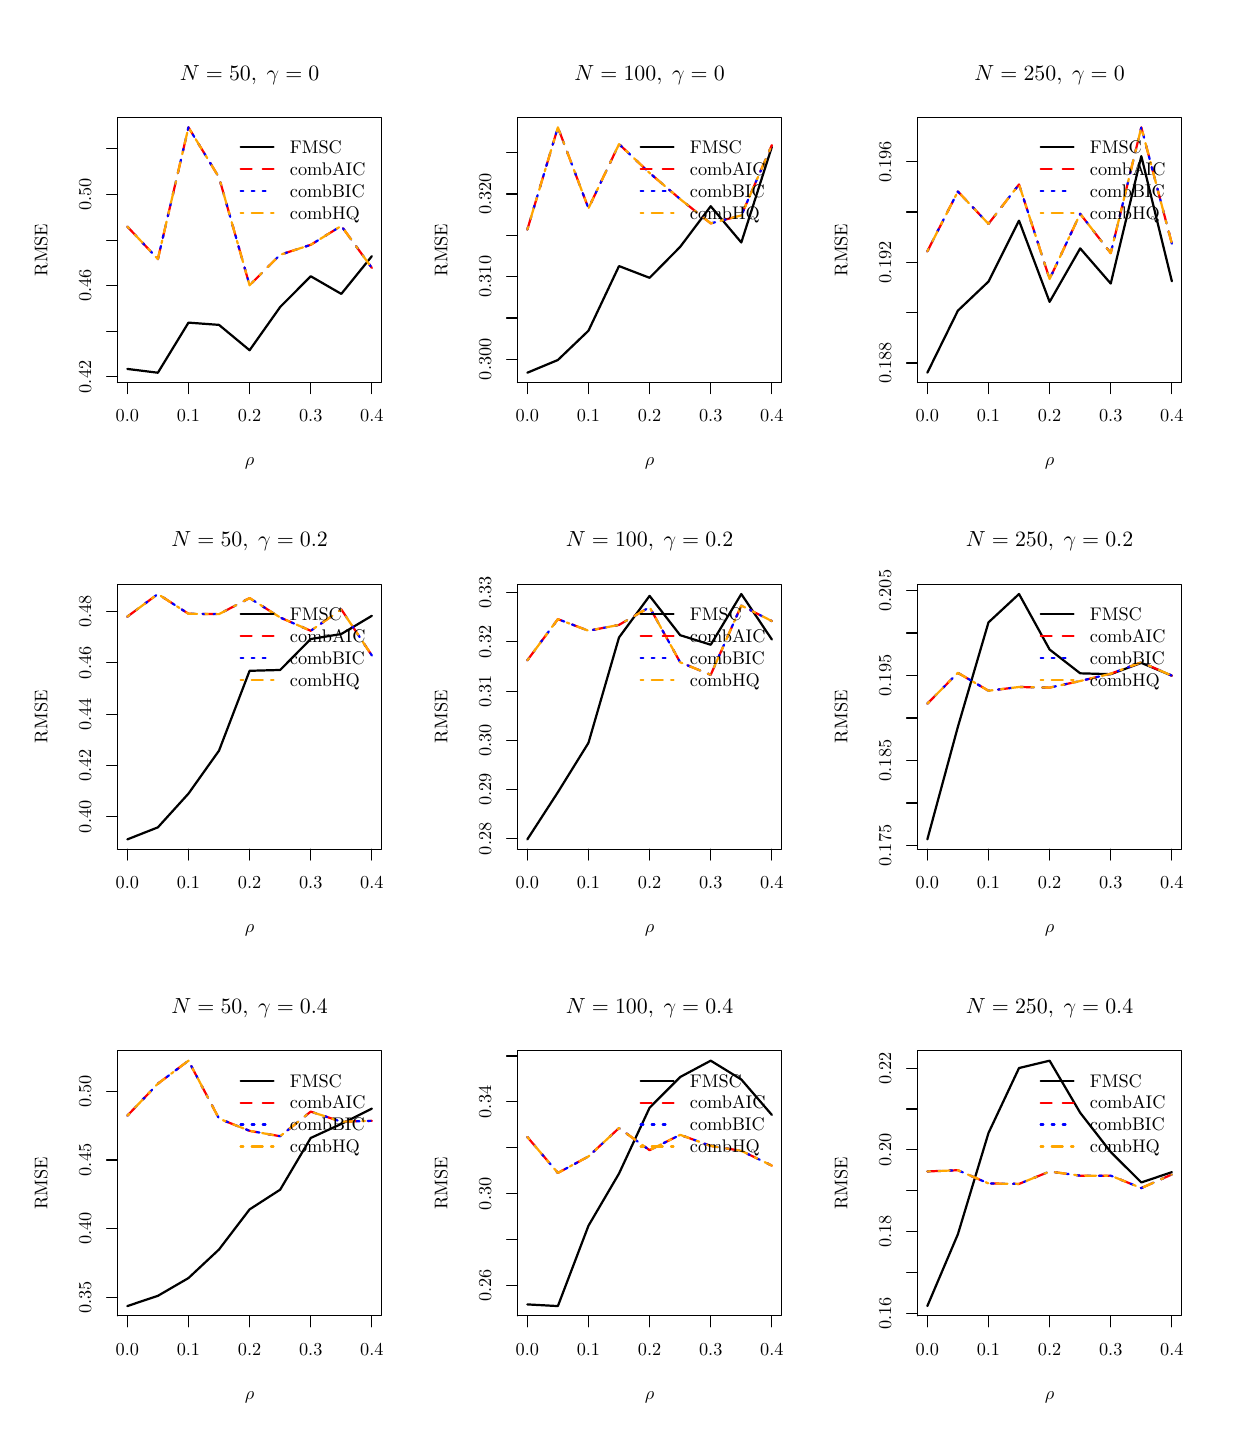
\begin{tikzpicture}[x=1pt,y=1pt]
\definecolor[named]{fillColor}{rgb}{1.00,1.00,1.00}
\path[use as bounding box,fill=fillColor,fill opacity=0.00] (0,0) rectangle (433.62,505.89);
\begin{scope}
\path[clip] ( 32.47,377.65) rectangle (127.91,473.42);
\definecolor[named]{drawColor}{rgb}{0.00,0.00,0.00}

\path[draw=drawColor,line width= 0.8pt,line join=round,line cap=round] ( 36.01,382.57) --
	( 47.05,381.20) --
	( 58.10,399.30) --
	( 69.14,398.49) --
	( 80.19,389.33) --
	( 91.24,404.95) --
	(102.28,416.06) --
	(113.33,409.68) --
	(124.37,423.32);
\end{scope}
\begin{scope}
\path[clip] (  0.00,  0.00) rectangle (433.62,505.89);
\definecolor[named]{drawColor}{rgb}{0.00,0.00,0.00}

\path[draw=drawColor,line width= 0.4pt,line join=round,line cap=round] ( 36.01,377.65) -- (124.37,377.65);

\path[draw=drawColor,line width= 0.4pt,line join=round,line cap=round] ( 36.01,377.65) -- ( 36.01,373.69);

\path[draw=drawColor,line width= 0.4pt,line join=round,line cap=round] ( 58.10,377.65) -- ( 58.10,373.69);

\path[draw=drawColor,line width= 0.4pt,line join=round,line cap=round] ( 80.19,377.65) -- ( 80.19,373.69);

\path[draw=drawColor,line width= 0.4pt,line join=round,line cap=round] (102.28,377.65) -- (102.28,373.69);

\path[draw=drawColor,line width= 0.4pt,line join=round,line cap=round] (124.37,377.65) -- (124.37,373.69);

\node[text=drawColor,anchor=base,inner sep=0pt, outer sep=0pt, scale=  0.66] at ( 36.01,363.40) {0.0};

\node[text=drawColor,anchor=base,inner sep=0pt, outer sep=0pt, scale=  0.66] at ( 58.10,363.40) {0.1};

\node[text=drawColor,anchor=base,inner sep=0pt, outer sep=0pt, scale=  0.66] at ( 80.19,363.40) {0.2};

\node[text=drawColor,anchor=base,inner sep=0pt, outer sep=0pt, scale=  0.66] at (102.28,363.40) {0.3};

\node[text=drawColor,anchor=base,inner sep=0pt, outer sep=0pt, scale=  0.66] at (124.37,363.40) {0.4};

\path[draw=drawColor,line width= 0.4pt,line join=round,line cap=round] ( 32.47,379.68) -- ( 32.47,462.08);

\path[draw=drawColor,line width= 0.4pt,line join=round,line cap=round] ( 32.47,379.68) -- ( 28.51,379.68);

\path[draw=drawColor,line width= 0.4pt,line join=round,line cap=round] ( 32.47,396.16) -- ( 28.51,396.16);

\path[draw=drawColor,line width= 0.4pt,line join=round,line cap=round] ( 32.47,412.64) -- ( 28.51,412.64);

\path[draw=drawColor,line width= 0.4pt,line join=round,line cap=round] ( 32.47,429.12) -- ( 28.51,429.12);

\path[draw=drawColor,line width= 0.4pt,line join=round,line cap=round] ( 32.47,445.60) -- ( 28.51,445.60);

\path[draw=drawColor,line width= 0.4pt,line join=round,line cap=round] ( 32.47,462.08) -- ( 28.51,462.08);

\node[text=drawColor,rotate= 90.00,anchor=base,inner sep=0pt, outer sep=0pt, scale=  0.66] at ( 22.97,379.68) {0.42};

\node[text=drawColor,rotate= 90.00,anchor=base,inner sep=0pt, outer sep=0pt, scale=  0.66] at ( 22.97,412.64) {0.46};

\node[text=drawColor,rotate= 90.00,anchor=base,inner sep=0pt, outer sep=0pt, scale=  0.66] at ( 22.97,445.60) {0.50};

\path[draw=drawColor,line width= 0.4pt,line join=round,line cap=round] ( 32.47,377.65) --
	(127.91,377.65) --
	(127.91,473.42) --
	( 32.47,473.42) --
	( 32.47,377.65);
\end{scope}
\begin{scope}
\path[clip] (  0.00,337.26) rectangle (144.54,505.89);
\definecolor[named]{drawColor}{rgb}{0.00,0.00,0.00}

\node[text=drawColor,anchor=base,inner sep=0pt, outer sep=0pt, scale=  0.79] at ( 80.19,486.92) {\bfseries $N=50, \;\gamma=0$};

\node[text=drawColor,anchor=base,inner sep=0pt, outer sep=0pt, scale=  0.66] at ( 80.19,347.56) {$\rho$};

\node[text=drawColor,rotate= 90.00,anchor=base,inner sep=0pt, outer sep=0pt, scale=  0.66] at (  7.13,425.53) {RMSE};
\end{scope}
\begin{scope}
\path[clip] ( 32.47,377.65) rectangle (127.91,473.42);
\definecolor[named]{drawColor}{rgb}{1.00,0.00,0.00}

\path[draw=drawColor,line width= 0.8pt,dash pattern=on 4pt off 4pt ,line join=round,line cap=round] ( 36.01,434.01) --
	( 47.05,422.27) --
	( 58.10,469.87) --
	( 69.14,451.78) --
	( 80.19,412.78) --
	( 91.24,423.83) --
	(102.28,427.41) --
	(113.33,434.25) --
	(124.37,419.07);
\definecolor[named]{drawColor}{rgb}{0.00,0.00,1.00}

\path[draw=drawColor,line width= 0.8pt,dash pattern=on 1pt off 3pt ,line join=round,line cap=round] ( 36.01,434.01) --
	( 47.05,422.27) --
	( 58.10,469.87) --
	( 69.14,451.78) --
	( 80.19,412.78) --
	( 91.24,423.83) --
	(102.28,427.41) --
	(113.33,434.25) --
	(124.37,419.07);
\definecolor[named]{drawColor}{rgb}{1.00,0.65,0.00}

\path[draw=drawColor,line width= 0.8pt,dash pattern=on 1pt off 3pt on 4pt off 3pt ,line join=round,line cap=round] ( 36.01,434.01) --
	( 47.05,422.27) --
	( 58.10,469.87) --
	( 69.14,451.78) --
	( 80.19,412.78) --
	( 91.24,423.83) --
	(102.28,427.41) --
	(113.33,434.25) --
	(124.37,419.07);
\definecolor[named]{drawColor}{rgb}{0.00,0.00,0.00}

\path[draw=drawColor,line width= 0.8pt,line join=round,line cap=round] ( 76.94,462.63) -- ( 88.82,462.63);
\definecolor[named]{drawColor}{rgb}{1.00,0.00,0.00}

\path[draw=drawColor,line width= 0.8pt,dash pattern=on 4pt off 4pt ,line join=round,line cap=round] ( 76.94,454.71) -- ( 88.82,454.71);
\definecolor[named]{drawColor}{rgb}{0.00,0.00,1.00}

\path[draw=drawColor,line width= 0.8pt,dash pattern=on 1pt off 3pt ,line join=round,line cap=round] ( 76.94,446.79) -- ( 88.82,446.79);
\definecolor[named]{drawColor}{rgb}{1.00,0.65,0.00}

\path[draw=drawColor,line width= 0.8pt,dash pattern=on 1pt off 3pt on 4pt off 3pt ,line join=round,line cap=round] ( 76.94,438.87) -- ( 88.82,438.87);
\definecolor[named]{drawColor}{rgb}{0.00,0.00,0.00}

\node[text=drawColor,anchor=base west,inner sep=0pt, outer sep=0pt, scale=  0.66] at ( 94.76,460.35) {FMSC};

\node[text=drawColor,anchor=base west,inner sep=0pt, outer sep=0pt, scale=  0.66] at ( 94.76,452.43) {combAIC};

\node[text=drawColor,anchor=base west,inner sep=0pt, outer sep=0pt, scale=  0.66] at ( 94.76,444.51) {combBIC};

\node[text=drawColor,anchor=base west,inner sep=0pt, outer sep=0pt, scale=  0.66] at ( 94.76,436.59) {combHQ};
\end{scope}
\begin{scope}
\path[clip] (177.01,377.65) rectangle (272.45,473.42);
\definecolor[named]{drawColor}{rgb}{0.00,0.00,0.00}

\path[draw=drawColor,line width= 0.8pt,line join=round,line cap=round] (180.55,381.20) --
	(191.59,385.80) --
	(202.64,396.38) --
	(213.68,419.74) --
	(224.73,415.49) --
	(235.78,426.69) --
	(246.82,441.36) --
	(257.87,428.26) --
	(268.91,462.83);
\end{scope}
\begin{scope}
\path[clip] (  0.00,  0.00) rectangle (433.62,505.89);
\definecolor[named]{drawColor}{rgb}{0.00,0.00,0.00}

\path[draw=drawColor,line width= 0.4pt,line join=round,line cap=round] (180.55,377.65) -- (268.91,377.65);

\path[draw=drawColor,line width= 0.4pt,line join=round,line cap=round] (180.55,377.65) -- (180.55,373.69);

\path[draw=drawColor,line width= 0.4pt,line join=round,line cap=round] (202.64,377.65) -- (202.64,373.69);

\path[draw=drawColor,line width= 0.4pt,line join=round,line cap=round] (224.73,377.65) -- (224.73,373.69);

\path[draw=drawColor,line width= 0.4pt,line join=round,line cap=round] (246.82,377.65) -- (246.82,373.69);

\path[draw=drawColor,line width= 0.4pt,line join=round,line cap=round] (268.91,377.65) -- (268.91,373.69);

\node[text=drawColor,anchor=base,inner sep=0pt, outer sep=0pt, scale=  0.66] at (180.55,363.40) {0.0};

\node[text=drawColor,anchor=base,inner sep=0pt, outer sep=0pt, scale=  0.66] at (202.64,363.40) {0.1};

\node[text=drawColor,anchor=base,inner sep=0pt, outer sep=0pt, scale=  0.66] at (224.73,363.40) {0.2};

\node[text=drawColor,anchor=base,inner sep=0pt, outer sep=0pt, scale=  0.66] at (246.82,363.40) {0.3};

\node[text=drawColor,anchor=base,inner sep=0pt, outer sep=0pt, scale=  0.66] at (268.91,363.40) {0.4};

\path[draw=drawColor,line width= 0.4pt,line join=round,line cap=round] (177.01,386.05) -- (177.01,460.74);

\path[draw=drawColor,line width= 0.4pt,line join=round,line cap=round] (177.01,386.05) -- (173.05,386.05);

\path[draw=drawColor,line width= 0.4pt,line join=round,line cap=round] (177.01,400.99) -- (173.05,400.99);

\path[draw=drawColor,line width= 0.4pt,line join=round,line cap=round] (177.01,415.92) -- (173.05,415.92);

\path[draw=drawColor,line width= 0.4pt,line join=round,line cap=round] (177.01,430.86) -- (173.05,430.86);

\path[draw=drawColor,line width= 0.4pt,line join=round,line cap=round] (177.01,445.80) -- (173.05,445.80);

\path[draw=drawColor,line width= 0.4pt,line join=round,line cap=round] (177.01,460.74) -- (173.05,460.74);

\node[text=drawColor,rotate= 90.00,anchor=base,inner sep=0pt, outer sep=0pt, scale=  0.66] at (167.51,386.05) {0.300};

\node[text=drawColor,rotate= 90.00,anchor=base,inner sep=0pt, outer sep=0pt, scale=  0.66] at (167.51,415.92) {0.310};

\node[text=drawColor,rotate= 90.00,anchor=base,inner sep=0pt, outer sep=0pt, scale=  0.66] at (167.51,445.80) {0.320};

\path[draw=drawColor,line width= 0.4pt,line join=round,line cap=round] (177.01,377.65) --
	(272.45,377.65) --
	(272.45,473.42) --
	(177.01,473.42) --
	(177.01,377.65);
\end{scope}
\begin{scope}
\path[clip] (144.54,337.26) rectangle (289.08,505.89);
\definecolor[named]{drawColor}{rgb}{0.00,0.00,0.00}

\node[text=drawColor,anchor=base,inner sep=0pt, outer sep=0pt, scale=  0.79] at (224.73,486.92) {\bfseries $N=100, \;\gamma=0$};

\node[text=drawColor,anchor=base,inner sep=0pt, outer sep=0pt, scale=  0.66] at (224.73,347.56) {$\rho$};

\node[text=drawColor,rotate= 90.00,anchor=base,inner sep=0pt, outer sep=0pt, scale=  0.66] at (151.67,425.54) {RMSE};
\end{scope}
\begin{scope}
\path[clip] (177.01,377.65) rectangle (272.45,473.42);
\definecolor[named]{drawColor}{rgb}{1.00,0.00,0.00}

\path[draw=drawColor,line width= 0.8pt,dash pattern=on 4pt off 4pt ,line join=round,line cap=round] (180.55,432.92) --
	(191.59,469.87) --
	(202.64,440.61) --
	(213.68,463.81) --
	(224.73,453.38) --
	(235.78,443.94) --
	(246.82,435.16) --
	(257.87,438.04) --
	(268.91,463.47);
\definecolor[named]{drawColor}{rgb}{0.00,0.00,1.00}

\path[draw=drawColor,line width= 0.8pt,dash pattern=on 1pt off 3pt ,line join=round,line cap=round] (180.55,432.92) --
	(191.59,469.87) --
	(202.64,440.61) --
	(213.68,463.81) --
	(224.73,453.38) --
	(235.78,443.94) --
	(246.82,435.16) --
	(257.87,438.04) --
	(268.91,463.47);
\definecolor[named]{drawColor}{rgb}{1.00,0.65,0.00}

\path[draw=drawColor,line width= 0.8pt,dash pattern=on 1pt off 3pt on 4pt off 3pt ,line join=round,line cap=round] (180.55,432.92) --
	(191.59,469.87) --
	(202.64,440.61) --
	(213.68,463.81) --
	(224.73,453.38) --
	(235.78,443.94) --
	(246.82,435.16) --
	(257.87,438.04) --
	(268.91,463.47);
\definecolor[named]{drawColor}{rgb}{0.00,0.00,0.00}

\path[draw=drawColor,line width= 0.8pt,line join=round,line cap=round] (221.48,462.63) -- (233.36,462.63);
\definecolor[named]{drawColor}{rgb}{1.00,0.00,0.00}

\path[draw=drawColor,line width= 0.8pt,dash pattern=on 4pt off 4pt ,line join=round,line cap=round] (221.48,454.71) -- (233.36,454.71);
\definecolor[named]{drawColor}{rgb}{0.00,0.00,1.00}

\path[draw=drawColor,line width= 0.8pt,dash pattern=on 1pt off 3pt ,line join=round,line cap=round] (221.48,446.79) -- (233.36,446.79);
\definecolor[named]{drawColor}{rgb}{1.00,0.65,0.00}

\path[draw=drawColor,line width= 0.8pt,dash pattern=on 1pt off 3pt on 4pt off 3pt ,line join=round,line cap=round] (221.48,438.87) -- (233.36,438.87);
\definecolor[named]{drawColor}{rgb}{0.00,0.00,0.00}

\node[text=drawColor,anchor=base west,inner sep=0pt, outer sep=0pt, scale=  0.66] at (239.30,460.35) {FMSC};

\node[text=drawColor,anchor=base west,inner sep=0pt, outer sep=0pt, scale=  0.66] at (239.30,452.43) {combAIC};

\node[text=drawColor,anchor=base west,inner sep=0pt, outer sep=0pt, scale=  0.66] at (239.30,444.51) {combBIC};

\node[text=drawColor,anchor=base west,inner sep=0pt, outer sep=0pt, scale=  0.66] at (239.30,436.59) {combHQ};
\end{scope}
\begin{scope}
\path[clip] (321.55,377.65) rectangle (416.99,473.42);
\definecolor[named]{drawColor}{rgb}{0.00,0.00,0.00}

\path[draw=drawColor,line width= 0.8pt,line join=round,line cap=round] (325.09,381.20) --
	(336.13,403.63) --
	(347.18,414.13) --
	(358.22,436.15) --
	(369.27,406.80) --
	(380.32,426.13) --
	(391.36,413.42) --
	(402.41,459.46) --
	(413.45,414.24);
\end{scope}
\begin{scope}
\path[clip] (  0.00,  0.00) rectangle (433.62,505.89);
\definecolor[named]{drawColor}{rgb}{0.00,0.00,0.00}

\path[draw=drawColor,line width= 0.4pt,line join=round,line cap=round] (325.09,377.65) -- (413.45,377.65);

\path[draw=drawColor,line width= 0.4pt,line join=round,line cap=round] (325.09,377.65) -- (325.09,373.69);

\path[draw=drawColor,line width= 0.4pt,line join=round,line cap=round] (347.18,377.65) -- (347.18,373.69);

\path[draw=drawColor,line width= 0.4pt,line join=round,line cap=round] (369.27,377.65) -- (369.27,373.69);

\path[draw=drawColor,line width= 0.4pt,line join=round,line cap=round] (391.36,377.65) -- (391.36,373.69);

\path[draw=drawColor,line width= 0.4pt,line join=round,line cap=round] (413.45,377.65) -- (413.45,373.69);

\node[text=drawColor,anchor=base,inner sep=0pt, outer sep=0pt, scale=  0.66] at (325.09,363.40) {0.0};

\node[text=drawColor,anchor=base,inner sep=0pt, outer sep=0pt, scale=  0.66] at (347.18,363.40) {0.1};

\node[text=drawColor,anchor=base,inner sep=0pt, outer sep=0pt, scale=  0.66] at (369.27,363.40) {0.2};

\node[text=drawColor,anchor=base,inner sep=0pt, outer sep=0pt, scale=  0.66] at (391.36,363.40) {0.3};

\node[text=drawColor,anchor=base,inner sep=0pt, outer sep=0pt, scale=  0.66] at (413.45,363.40) {0.4};

\path[draw=drawColor,line width= 0.4pt,line join=round,line cap=round] (321.55,384.73) -- (321.55,457.44);

\path[draw=drawColor,line width= 0.4pt,line join=round,line cap=round] (321.55,384.73) -- (317.59,384.73);

\path[draw=drawColor,line width= 0.4pt,line join=round,line cap=round] (321.55,402.91) -- (317.59,402.91);

\path[draw=drawColor,line width= 0.4pt,line join=round,line cap=round] (321.55,421.08) -- (317.59,421.08);

\path[draw=drawColor,line width= 0.4pt,line join=round,line cap=round] (321.55,439.26) -- (317.59,439.26);

\path[draw=drawColor,line width= 0.4pt,line join=round,line cap=round] (321.55,457.44) -- (317.59,457.44);

\node[text=drawColor,rotate= 90.00,anchor=base,inner sep=0pt, outer sep=0pt, scale=  0.66] at (312.05,384.73) {0.188};

\node[text=drawColor,rotate= 90.00,anchor=base,inner sep=0pt, outer sep=0pt, scale=  0.66] at (312.05,421.08) {0.192};

\node[text=drawColor,rotate= 90.00,anchor=base,inner sep=0pt, outer sep=0pt, scale=  0.66] at (312.05,457.44) {0.196};

\path[draw=drawColor,line width= 0.4pt,line join=round,line cap=round] (321.55,377.65) --
	(416.99,377.65) --
	(416.99,473.42) --
	(321.55,473.42) --
	(321.55,377.65);
\end{scope}
\begin{scope}
\path[clip] (289.08,337.26) rectangle (433.62,505.89);
\definecolor[named]{drawColor}{rgb}{0.00,0.00,0.00}

\node[text=drawColor,anchor=base,inner sep=0pt, outer sep=0pt, scale=  0.79] at (369.27,486.92) {\bfseries $N=250, \;\gamma=0$};

\node[text=drawColor,anchor=base,inner sep=0pt, outer sep=0pt, scale=  0.66] at (369.27,347.56) {$\rho$};

\node[text=drawColor,rotate= 90.00,anchor=base,inner sep=0pt, outer sep=0pt, scale=  0.66] at (296.21,425.53) {RMSE};
\end{scope}
\begin{scope}
\path[clip] (321.55,377.65) rectangle (416.99,473.42);
\definecolor[named]{drawColor}{rgb}{1.00,0.00,0.00}

\path[draw=drawColor,line width= 0.8pt,dash pattern=on 4pt off 4pt ,line join=round,line cap=round] (325.09,425.07) --
	(336.13,446.68) --
	(347.18,435.00) --
	(358.22,449.24) --
	(369.27,415.06) --
	(380.32,438.63) --
	(391.36,424.40) --
	(402.41,469.87) --
	(413.45,427.83);
\definecolor[named]{drawColor}{rgb}{0.00,0.00,1.00}

\path[draw=drawColor,line width= 0.8pt,dash pattern=on 1pt off 3pt ,line join=round,line cap=round] (325.09,425.07) --
	(336.13,446.68) --
	(347.18,435.00) --
	(358.22,449.24) --
	(369.27,415.06) --
	(380.32,438.63) --
	(391.36,424.40) --
	(402.41,469.87) --
	(413.45,427.83);
\definecolor[named]{drawColor}{rgb}{1.00,0.65,0.00}

\path[draw=drawColor,line width= 0.8pt,dash pattern=on 1pt off 3pt on 4pt off 3pt ,line join=round,line cap=round] (325.09,425.07) --
	(336.13,446.68) --
	(347.18,435.00) --
	(358.22,449.24) --
	(369.27,415.06) --
	(380.32,438.63) --
	(391.36,424.40) --
	(402.41,469.87) --
	(413.45,427.83);
\definecolor[named]{drawColor}{rgb}{0.00,0.00,0.00}

\path[draw=drawColor,line width= 0.8pt,line join=round,line cap=round] (366.02,462.63) -- (377.90,462.63);
\definecolor[named]{drawColor}{rgb}{1.00,0.00,0.00}

\path[draw=drawColor,line width= 0.8pt,dash pattern=on 4pt off 4pt ,line join=round,line cap=round] (366.02,454.71) -- (377.90,454.71);
\definecolor[named]{drawColor}{rgb}{0.00,0.00,1.00}

\path[draw=drawColor,line width= 0.8pt,dash pattern=on 1pt off 3pt ,line join=round,line cap=round] (366.02,446.79) -- (377.90,446.79);
\definecolor[named]{drawColor}{rgb}{1.00,0.65,0.00}

\path[draw=drawColor,line width= 0.8pt,dash pattern=on 1pt off 3pt on 4pt off 3pt ,line join=round,line cap=round] (366.02,438.87) -- (377.90,438.87);
\definecolor[named]{drawColor}{rgb}{0.00,0.00,0.00}

\node[text=drawColor,anchor=base west,inner sep=0pt, outer sep=0pt, scale=  0.66] at (383.84,460.35) {FMSC};

\node[text=drawColor,anchor=base west,inner sep=0pt, outer sep=0pt, scale=  0.66] at (383.84,452.43) {combAIC};

\node[text=drawColor,anchor=base west,inner sep=0pt, outer sep=0pt, scale=  0.66] at (383.84,444.51) {combBIC};

\node[text=drawColor,anchor=base west,inner sep=0pt, outer sep=0pt, scale=  0.66] at (383.84,436.59) {combHQ};
\end{scope}
\begin{scope}
\path[clip] ( 32.47,209.02) rectangle (127.91,304.79);
\definecolor[named]{drawColor}{rgb}{0.00,0.00,0.00}

\path[draw=drawColor,line width= 0.8pt,line join=round,line cap=round] ( 36.01,212.57) --
	( 47.05,216.92) --
	( 58.10,229.11) --
	( 69.14,244.64) --
	( 80.19,273.49) --
	( 91.24,273.79) --
	(102.28,284.97) --
	(113.33,286.79) --
	(124.37,293.36);
\end{scope}
\begin{scope}
\path[clip] (  0.00,  0.00) rectangle (433.62,505.89);
\definecolor[named]{drawColor}{rgb}{0.00,0.00,0.00}

\path[draw=drawColor,line width= 0.4pt,line join=round,line cap=round] ( 36.01,209.02) -- (124.37,209.02);

\path[draw=drawColor,line width= 0.4pt,line join=round,line cap=round] ( 36.01,209.02) -- ( 36.01,205.06);

\path[draw=drawColor,line width= 0.4pt,line join=round,line cap=round] ( 58.10,209.02) -- ( 58.10,205.06);

\path[draw=drawColor,line width= 0.4pt,line join=round,line cap=round] ( 80.19,209.02) -- ( 80.19,205.06);

\path[draw=drawColor,line width= 0.4pt,line join=round,line cap=round] (102.28,209.02) -- (102.28,205.06);

\path[draw=drawColor,line width= 0.4pt,line join=round,line cap=round] (124.37,209.02) -- (124.37,205.06);

\node[text=drawColor,anchor=base,inner sep=0pt, outer sep=0pt, scale=  0.66] at ( 36.01,194.77) {0.0};

\node[text=drawColor,anchor=base,inner sep=0pt, outer sep=0pt, scale=  0.66] at ( 58.10,194.77) {0.1};

\node[text=drawColor,anchor=base,inner sep=0pt, outer sep=0pt, scale=  0.66] at ( 80.19,194.77) {0.2};

\node[text=drawColor,anchor=base,inner sep=0pt, outer sep=0pt, scale=  0.66] at (102.28,194.77) {0.3};

\node[text=drawColor,anchor=base,inner sep=0pt, outer sep=0pt, scale=  0.66] at (124.37,194.77) {0.4};

\path[draw=drawColor,line width= 0.4pt,line join=round,line cap=round] ( 32.47,220.75) -- ( 32.47,294.93);

\path[draw=drawColor,line width= 0.4pt,line join=round,line cap=round] ( 32.47,220.75) -- ( 28.51,220.75);

\path[draw=drawColor,line width= 0.4pt,line join=round,line cap=round] ( 32.47,239.29) -- ( 28.51,239.29);

\path[draw=drawColor,line width= 0.4pt,line join=round,line cap=round] ( 32.47,257.84) -- ( 28.51,257.84);

\path[draw=drawColor,line width= 0.4pt,line join=round,line cap=round] ( 32.47,276.38) -- ( 28.51,276.38);

\path[draw=drawColor,line width= 0.4pt,line join=round,line cap=round] ( 32.47,294.93) -- ( 28.51,294.93);

\node[text=drawColor,rotate= 90.00,anchor=base,inner sep=0pt, outer sep=0pt, scale=  0.66] at ( 22.97,220.75) {0.40};

\node[text=drawColor,rotate= 90.00,anchor=base,inner sep=0pt, outer sep=0pt, scale=  0.66] at ( 22.97,239.29) {0.42};

\node[text=drawColor,rotate= 90.00,anchor=base,inner sep=0pt, outer sep=0pt, scale=  0.66] at ( 22.97,257.84) {0.44};

\node[text=drawColor,rotate= 90.00,anchor=base,inner sep=0pt, outer sep=0pt, scale=  0.66] at ( 22.97,276.38) {0.46};

\node[text=drawColor,rotate= 90.00,anchor=base,inner sep=0pt, outer sep=0pt, scale=  0.66] at ( 22.97,294.93) {0.48};

\path[draw=drawColor,line width= 0.4pt,line join=round,line cap=round] ( 32.47,209.02) --
	(127.91,209.02) --
	(127.91,304.79) --
	( 32.47,304.79) --
	( 32.47,209.02);
\end{scope}
\begin{scope}
\path[clip] (  0.00,168.63) rectangle (144.54,337.26);
\definecolor[named]{drawColor}{rgb}{0.00,0.00,0.00}

\node[text=drawColor,anchor=base,inner sep=0pt, outer sep=0pt, scale=  0.79] at ( 80.19,318.29) {\bfseries $N=50, \;\gamma=0.2$};

\node[text=drawColor,anchor=base,inner sep=0pt, outer sep=0pt, scale=  0.66] at ( 80.19,178.93) {$\rho$};

\node[text=drawColor,rotate= 90.00,anchor=base,inner sep=0pt, outer sep=0pt, scale=  0.66] at (  7.13,256.90) {RMSE};
\end{scope}
\begin{scope}
\path[clip] ( 32.47,209.02) rectangle (127.91,304.79);
\definecolor[named]{drawColor}{rgb}{1.00,0.00,0.00}

\path[draw=drawColor,line width= 0.8pt,dash pattern=on 4pt off 4pt ,line join=round,line cap=round] ( 36.01,293.06) --
	( 47.05,301.24) --
	( 58.10,294.10) --
	( 69.14,293.97) --
	( 80.19,299.77) --
	( 91.24,292.76) --
	(102.28,287.95) --
	(113.33,295.67) --
	(124.37,279.02);
\definecolor[named]{drawColor}{rgb}{0.00,0.00,1.00}

\path[draw=drawColor,line width= 0.8pt,dash pattern=on 1pt off 3pt ,line join=round,line cap=round] ( 36.01,293.06) --
	( 47.05,301.24) --
	( 58.10,294.10) --
	( 69.14,293.97) --
	( 80.19,299.77) --
	( 91.24,292.76) --
	(102.28,287.95) --
	(113.33,295.67) --
	(124.37,279.02);
\definecolor[named]{drawColor}{rgb}{1.00,0.65,0.00}

\path[draw=drawColor,line width= 0.8pt,dash pattern=on 1pt off 3pt on 4pt off 3pt ,line join=round,line cap=round] ( 36.01,293.06) --
	( 47.05,301.24) --
	( 58.10,294.10) --
	( 69.14,293.97) --
	( 80.19,299.77) --
	( 91.24,292.76) --
	(102.28,287.95) --
	(113.33,295.67) --
	(124.37,279.02);
\definecolor[named]{drawColor}{rgb}{0.00,0.00,0.00}

\path[draw=drawColor,line width= 0.8pt,line join=round,line cap=round] ( 76.94,294.00) -- ( 88.82,294.00);
\definecolor[named]{drawColor}{rgb}{1.00,0.00,0.00}

\path[draw=drawColor,line width= 0.8pt,dash pattern=on 4pt off 4pt ,line join=round,line cap=round] ( 76.94,286.08) -- ( 88.82,286.08);
\definecolor[named]{drawColor}{rgb}{0.00,0.00,1.00}

\path[draw=drawColor,line width= 0.8pt,dash pattern=on 1pt off 3pt ,line join=round,line cap=round] ( 76.94,278.16) -- ( 88.82,278.16);
\definecolor[named]{drawColor}{rgb}{1.00,0.65,0.00}

\path[draw=drawColor,line width= 0.8pt,dash pattern=on 1pt off 3pt on 4pt off 3pt ,line join=round,line cap=round] ( 76.94,270.24) -- ( 88.82,270.24);
\definecolor[named]{drawColor}{rgb}{0.00,0.00,0.00}

\node[text=drawColor,anchor=base west,inner sep=0pt, outer sep=0pt, scale=  0.66] at ( 94.76,291.72) {FMSC};

\node[text=drawColor,anchor=base west,inner sep=0pt, outer sep=0pt, scale=  0.66] at ( 94.76,283.80) {combAIC};

\node[text=drawColor,anchor=base west,inner sep=0pt, outer sep=0pt, scale=  0.66] at ( 94.76,275.88) {combBIC};

\node[text=drawColor,anchor=base west,inner sep=0pt, outer sep=0pt, scale=  0.66] at ( 94.76,267.96) {combHQ};
\end{scope}
\begin{scope}
\path[clip] (177.01,209.02) rectangle (272.45,304.79);
\definecolor[named]{drawColor}{rgb}{0.00,0.00,0.00}

\path[draw=drawColor,line width= 0.8pt,line join=round,line cap=round] (180.55,212.57) --
	(191.59,229.62) --
	(202.64,247.45) --
	(213.68,285.54) --
	(224.73,300.57) --
	(235.78,286.36) --
	(246.82,282.91) --
	(257.87,301.24) --
	(268.91,284.80);
\end{scope}
\begin{scope}
\path[clip] (  0.00,  0.00) rectangle (433.62,505.89);
\definecolor[named]{drawColor}{rgb}{0.00,0.00,0.00}

\path[draw=drawColor,line width= 0.4pt,line join=round,line cap=round] (180.55,209.02) -- (268.91,209.02);

\path[draw=drawColor,line width= 0.4pt,line join=round,line cap=round] (180.55,209.02) -- (180.55,205.06);

\path[draw=drawColor,line width= 0.4pt,line join=round,line cap=round] (202.64,209.02) -- (202.64,205.06);

\path[draw=drawColor,line width= 0.4pt,line join=round,line cap=round] (224.73,209.02) -- (224.73,205.06);

\path[draw=drawColor,line width= 0.4pt,line join=round,line cap=round] (246.82,209.02) -- (246.82,205.06);

\path[draw=drawColor,line width= 0.4pt,line join=round,line cap=round] (268.91,209.02) -- (268.91,205.06);

\node[text=drawColor,anchor=base,inner sep=0pt, outer sep=0pt, scale=  0.66] at (180.55,194.77) {0.0};

\node[text=drawColor,anchor=base,inner sep=0pt, outer sep=0pt, scale=  0.66] at (202.64,194.77) {0.1};

\node[text=drawColor,anchor=base,inner sep=0pt, outer sep=0pt, scale=  0.66] at (224.73,194.77) {0.2};

\node[text=drawColor,anchor=base,inner sep=0pt, outer sep=0pt, scale=  0.66] at (246.82,194.77) {0.3};

\node[text=drawColor,anchor=base,inner sep=0pt, outer sep=0pt, scale=  0.66] at (268.91,194.77) {0.4};

\path[draw=drawColor,line width= 0.4pt,line join=round,line cap=round] (177.01,212.80) -- (177.01,301.70);

\path[draw=drawColor,line width= 0.4pt,line join=round,line cap=round] (177.01,212.80) -- (173.05,212.80);

\path[draw=drawColor,line width= 0.4pt,line join=round,line cap=round] (177.01,230.58) -- (173.05,230.58);

\path[draw=drawColor,line width= 0.4pt,line join=round,line cap=round] (177.01,248.36) -- (173.05,248.36);

\path[draw=drawColor,line width= 0.4pt,line join=round,line cap=round] (177.01,266.14) -- (173.05,266.14);

\path[draw=drawColor,line width= 0.4pt,line join=round,line cap=round] (177.01,283.92) -- (173.05,283.92);

\path[draw=drawColor,line width= 0.4pt,line join=round,line cap=round] (177.01,301.70) -- (173.05,301.70);

\node[text=drawColor,rotate= 90.00,anchor=base,inner sep=0pt, outer sep=0pt, scale=  0.66] at (167.51,212.80) {0.28};

\node[text=drawColor,rotate= 90.00,anchor=base,inner sep=0pt, outer sep=0pt, scale=  0.66] at (167.51,230.58) {0.29};

\node[text=drawColor,rotate= 90.00,anchor=base,inner sep=0pt, outer sep=0pt, scale=  0.66] at (167.51,248.36) {0.30};

\node[text=drawColor,rotate= 90.00,anchor=base,inner sep=0pt, outer sep=0pt, scale=  0.66] at (167.51,266.14) {0.31};

\node[text=drawColor,rotate= 90.00,anchor=base,inner sep=0pt, outer sep=0pt, scale=  0.66] at (167.51,283.92) {0.32};

\node[text=drawColor,rotate= 90.00,anchor=base,inner sep=0pt, outer sep=0pt, scale=  0.66] at (167.51,301.70) {0.33};

\path[draw=drawColor,line width= 0.4pt,line join=round,line cap=round] (177.01,209.02) --
	(272.45,209.02) --
	(272.45,304.79) --
	(177.01,304.79) --
	(177.01,209.02);
\end{scope}
\begin{scope}
\path[clip] (144.54,168.63) rectangle (289.08,337.26);
\definecolor[named]{drawColor}{rgb}{0.00,0.00,0.00}

\node[text=drawColor,anchor=base,inner sep=0pt, outer sep=0pt, scale=  0.79] at (224.73,318.29) {\bfseries $N=100, \;\gamma=0.2$};

\node[text=drawColor,anchor=base,inner sep=0pt, outer sep=0pt, scale=  0.66] at (224.73,178.93) {$\rho$};

\node[text=drawColor,rotate= 90.00,anchor=base,inner sep=0pt, outer sep=0pt, scale=  0.66] at (151.67,256.90) {RMSE};
\end{scope}
\begin{scope}
\path[clip] (177.01,209.02) rectangle (272.45,304.79);
\definecolor[named]{drawColor}{rgb}{1.00,0.00,0.00}

\path[draw=drawColor,line width= 0.8pt,dash pattern=on 4pt off 4pt ,line join=round,line cap=round] (180.55,277.28) --
	(191.59,292.16) --
	(202.64,287.97) --
	(213.68,290.08) --
	(224.73,296.49) --
	(235.78,276.56) --
	(246.82,272.04) --
	(257.87,297.07) --
	(268.91,291.46);
\definecolor[named]{drawColor}{rgb}{0.00,0.00,1.00}

\path[draw=drawColor,line width= 0.8pt,dash pattern=on 1pt off 3pt ,line join=round,line cap=round] (180.55,277.28) --
	(191.59,292.16) --
	(202.64,287.97) --
	(213.68,290.08) --
	(224.73,296.49) --
	(235.78,276.56) --
	(246.82,272.04) --
	(257.87,297.07) --
	(268.91,291.46);
\definecolor[named]{drawColor}{rgb}{1.00,0.65,0.00}

\path[draw=drawColor,line width= 0.8pt,dash pattern=on 1pt off 3pt on 4pt off 3pt ,line join=round,line cap=round] (180.55,277.28) --
	(191.59,292.16) --
	(202.64,287.97) --
	(213.68,290.08) --
	(224.73,296.49) --
	(235.78,276.56) --
	(246.82,272.04) --
	(257.87,297.07) --
	(268.91,291.46);
\definecolor[named]{drawColor}{rgb}{0.00,0.00,0.00}

\path[draw=drawColor,line width= 0.8pt,line join=round,line cap=round] (221.48,294.00) -- (233.36,294.00);
\definecolor[named]{drawColor}{rgb}{1.00,0.00,0.00}

\path[draw=drawColor,line width= 0.8pt,dash pattern=on 4pt off 4pt ,line join=round,line cap=round] (221.48,286.08) -- (233.36,286.08);
\definecolor[named]{drawColor}{rgb}{0.00,0.00,1.00}

\path[draw=drawColor,line width= 0.8pt,dash pattern=on 1pt off 3pt ,line join=round,line cap=round] (221.48,278.16) -- (233.36,278.16);
\definecolor[named]{drawColor}{rgb}{1.00,0.65,0.00}

\path[draw=drawColor,line width= 0.8pt,dash pattern=on 1pt off 3pt on 4pt off 3pt ,line join=round,line cap=round] (221.48,270.24) -- (233.36,270.24);
\definecolor[named]{drawColor}{rgb}{0.00,0.00,0.00}

\node[text=drawColor,anchor=base west,inner sep=0pt, outer sep=0pt, scale=  0.66] at (239.30,291.72) {FMSC};

\node[text=drawColor,anchor=base west,inner sep=0pt, outer sep=0pt, scale=  0.66] at (239.30,283.80) {combAIC};

\node[text=drawColor,anchor=base west,inner sep=0pt, outer sep=0pt, scale=  0.66] at (239.30,275.88) {combBIC};

\node[text=drawColor,anchor=base west,inner sep=0pt, outer sep=0pt, scale=  0.66] at (239.30,267.96) {combHQ};
\end{scope}
\begin{scope}
\path[clip] (321.55,209.02) rectangle (416.99,304.79);
\definecolor[named]{drawColor}{rgb}{0.00,0.00,0.00}

\path[draw=drawColor,line width= 0.8pt,line join=round,line cap=round] (325.09,212.57) --
	(336.13,253.26) --
	(347.18,290.98) --
	(358.22,301.24) --
	(369.27,281.18) --
	(380.32,272.58) --
	(391.36,272.27) --
	(402.41,276.35) --
	(413.45,271.73);
\end{scope}
\begin{scope}
\path[clip] (  0.00,  0.00) rectangle (433.62,505.89);
\definecolor[named]{drawColor}{rgb}{0.00,0.00,0.00}

\path[draw=drawColor,line width= 0.4pt,line join=round,line cap=round] (325.09,209.02) -- (413.45,209.02);

\path[draw=drawColor,line width= 0.4pt,line join=round,line cap=round] (325.09,209.02) -- (325.09,205.06);

\path[draw=drawColor,line width= 0.4pt,line join=round,line cap=round] (347.18,209.02) -- (347.18,205.06);

\path[draw=drawColor,line width= 0.4pt,line join=round,line cap=round] (369.27,209.02) -- (369.27,205.06);

\path[draw=drawColor,line width= 0.4pt,line join=round,line cap=round] (391.36,209.02) -- (391.36,205.06);

\path[draw=drawColor,line width= 0.4pt,line join=round,line cap=round] (413.45,209.02) -- (413.45,205.06);

\node[text=drawColor,anchor=base,inner sep=0pt, outer sep=0pt, scale=  0.66] at (325.09,194.77) {0.0};

\node[text=drawColor,anchor=base,inner sep=0pt, outer sep=0pt, scale=  0.66] at (347.18,194.77) {0.1};

\node[text=drawColor,anchor=base,inner sep=0pt, outer sep=0pt, scale=  0.66] at (369.27,194.77) {0.2};

\node[text=drawColor,anchor=base,inner sep=0pt, outer sep=0pt, scale=  0.66] at (391.36,194.77) {0.3};

\node[text=drawColor,anchor=base,inner sep=0pt, outer sep=0pt, scale=  0.66] at (413.45,194.77) {0.4};

\path[draw=drawColor,line width= 0.4pt,line join=round,line cap=round] (321.55,210.39) -- (321.55,302.49);

\path[draw=drawColor,line width= 0.4pt,line join=round,line cap=round] (321.55,210.39) -- (317.59,210.39);

\path[draw=drawColor,line width= 0.4pt,line join=round,line cap=round] (321.55,225.74) -- (317.59,225.74);

\path[draw=drawColor,line width= 0.4pt,line join=round,line cap=round] (321.55,241.09) -- (317.59,241.09);

\path[draw=drawColor,line width= 0.4pt,line join=round,line cap=round] (321.55,256.44) -- (317.59,256.44);

\path[draw=drawColor,line width= 0.4pt,line join=round,line cap=round] (321.55,271.79) -- (317.59,271.79);

\path[draw=drawColor,line width= 0.4pt,line join=round,line cap=round] (321.55,287.14) -- (317.59,287.14);

\path[draw=drawColor,line width= 0.4pt,line join=round,line cap=round] (321.55,302.49) -- (317.59,302.49);

\node[text=drawColor,rotate= 90.00,anchor=base,inner sep=0pt, outer sep=0pt, scale=  0.66] at (312.05,210.39) {0.175};

\node[text=drawColor,rotate= 90.00,anchor=base,inner sep=0pt, outer sep=0pt, scale=  0.66] at (312.05,241.09) {0.185};

\node[text=drawColor,rotate= 90.00,anchor=base,inner sep=0pt, outer sep=0pt, scale=  0.66] at (312.05,271.79) {0.195};

\node[text=drawColor,rotate= 90.00,anchor=base,inner sep=0pt, outer sep=0pt, scale=  0.66] at (312.05,302.49) {0.205};

\path[draw=drawColor,line width= 0.4pt,line join=round,line cap=round] (321.55,209.02) --
	(416.99,209.02) --
	(416.99,304.79) --
	(321.55,304.79) --
	(321.55,209.02);
\end{scope}
\begin{scope}
\path[clip] (289.08,168.63) rectangle (433.62,337.26);
\definecolor[named]{drawColor}{rgb}{0.00,0.00,0.00}

\node[text=drawColor,anchor=base,inner sep=0pt, outer sep=0pt, scale=  0.79] at (369.27,318.29) {\bfseries $N=250, \;\gamma=0.2$};

\node[text=drawColor,anchor=base,inner sep=0pt, outer sep=0pt, scale=  0.66] at (369.27,178.93) {$\rho$};

\node[text=drawColor,rotate= 90.00,anchor=base,inner sep=0pt, outer sep=0pt, scale=  0.66] at (296.21,256.90) {RMSE};
\end{scope}
\begin{scope}
\path[clip] (321.55,209.02) rectangle (416.99,304.79);
\definecolor[named]{drawColor}{rgb}{1.00,0.00,0.00}

\path[draw=drawColor,line width= 0.8pt,dash pattern=on 4pt off 4pt ,line join=round,line cap=round] (325.09,261.62) --
	(336.13,272.76) --
	(347.18,266.29) --
	(358.22,267.64) --
	(369.27,267.41) --
	(380.32,269.80) --
	(391.36,272.43) --
	(402.41,276.55) --
	(413.45,271.74);
\definecolor[named]{drawColor}{rgb}{0.00,0.00,1.00}

\path[draw=drawColor,line width= 0.8pt,dash pattern=on 1pt off 3pt ,line join=round,line cap=round] (325.09,261.62) --
	(336.13,272.76) --
	(347.18,266.29) --
	(358.22,267.64) --
	(369.27,267.41) --
	(380.32,269.80) --
	(391.36,272.43) --
	(402.41,276.55) --
	(413.45,271.74);
\definecolor[named]{drawColor}{rgb}{1.00,0.65,0.00}

\path[draw=drawColor,line width= 0.8pt,dash pattern=on 1pt off 3pt on 4pt off 3pt ,line join=round,line cap=round] (325.09,261.62) --
	(336.13,272.76) --
	(347.18,266.29) --
	(358.22,267.64) --
	(369.27,267.41) --
	(380.32,269.80) --
	(391.36,272.43) --
	(402.41,276.55) --
	(413.45,271.74);
\definecolor[named]{drawColor}{rgb}{0.00,0.00,0.00}

\path[draw=drawColor,line width= 0.8pt,line join=round,line cap=round] (366.02,294.00) -- (377.90,294.00);
\definecolor[named]{drawColor}{rgb}{1.00,0.00,0.00}

\path[draw=drawColor,line width= 0.8pt,dash pattern=on 4pt off 4pt ,line join=round,line cap=round] (366.02,286.08) -- (377.90,286.08);
\definecolor[named]{drawColor}{rgb}{0.00,0.00,1.00}

\path[draw=drawColor,line width= 0.8pt,dash pattern=on 1pt off 3pt ,line join=round,line cap=round] (366.02,278.16) -- (377.90,278.16);
\definecolor[named]{drawColor}{rgb}{1.00,0.65,0.00}

\path[draw=drawColor,line width= 0.8pt,dash pattern=on 1pt off 3pt on 4pt off 3pt ,line join=round,line cap=round] (366.02,270.24) -- (377.90,270.24);
\definecolor[named]{drawColor}{rgb}{0.00,0.00,0.00}

\node[text=drawColor,anchor=base west,inner sep=0pt, outer sep=0pt, scale=  0.66] at (383.84,291.72) {FMSC};

\node[text=drawColor,anchor=base west,inner sep=0pt, outer sep=0pt, scale=  0.66] at (383.84,283.80) {combAIC};

\node[text=drawColor,anchor=base west,inner sep=0pt, outer sep=0pt, scale=  0.66] at (383.84,275.88) {combBIC};

\node[text=drawColor,anchor=base west,inner sep=0pt, outer sep=0pt, scale=  0.66] at (383.84,267.96) {combHQ};
\end{scope}
\begin{scope}
\path[clip] ( 32.47, 40.39) rectangle (127.91,136.16);
\definecolor[named]{drawColor}{rgb}{0.00,0.00,0.00}

\path[draw=drawColor,line width= 0.8pt,line join=round,line cap=round] ( 36.01, 43.94) --
	( 47.05, 47.64) --
	( 58.10, 54.06) --
	( 69.14, 64.39) --
	( 80.19, 78.87) --
	( 91.24, 86.00) --
	(102.28,104.68) --
	(113.33,109.76) --
	(124.37,115.30);
\end{scope}
\begin{scope}
\path[clip] (  0.00,  0.00) rectangle (433.62,505.89);
\definecolor[named]{drawColor}{rgb}{0.00,0.00,0.00}

\path[draw=drawColor,line width= 0.4pt,line join=round,line cap=round] ( 36.01, 40.39) -- (124.37, 40.39);

\path[draw=drawColor,line width= 0.4pt,line join=round,line cap=round] ( 36.01, 40.39) -- ( 36.01, 36.43);

\path[draw=drawColor,line width= 0.4pt,line join=round,line cap=round] ( 58.10, 40.39) -- ( 58.10, 36.43);

\path[draw=drawColor,line width= 0.4pt,line join=round,line cap=round] ( 80.19, 40.39) -- ( 80.19, 36.43);

\path[draw=drawColor,line width= 0.4pt,line join=round,line cap=round] (102.28, 40.39) -- (102.28, 36.43);

\path[draw=drawColor,line width= 0.4pt,line join=round,line cap=round] (124.37, 40.39) -- (124.37, 36.43);

\node[text=drawColor,anchor=base,inner sep=0pt, outer sep=0pt, scale=  0.66] at ( 36.01, 26.14) {0.0};

\node[text=drawColor,anchor=base,inner sep=0pt, outer sep=0pt, scale=  0.66] at ( 58.10, 26.14) {0.1};

\node[text=drawColor,anchor=base,inner sep=0pt, outer sep=0pt, scale=  0.66] at ( 80.19, 26.14) {0.2};

\node[text=drawColor,anchor=base,inner sep=0pt, outer sep=0pt, scale=  0.66] at (102.28, 26.14) {0.3};

\node[text=drawColor,anchor=base,inner sep=0pt, outer sep=0pt, scale=  0.66] at (124.37, 26.14) {0.4};

\path[draw=drawColor,line width= 0.4pt,line join=round,line cap=round] ( 32.47, 47.06) -- ( 32.47,121.59);

\path[draw=drawColor,line width= 0.4pt,line join=round,line cap=round] ( 32.47, 47.06) -- ( 28.51, 47.06);

\path[draw=drawColor,line width= 0.4pt,line join=round,line cap=round] ( 32.47, 71.90) -- ( 28.51, 71.90);

\path[draw=drawColor,line width= 0.4pt,line join=round,line cap=round] ( 32.47, 96.74) -- ( 28.51, 96.74);

\path[draw=drawColor,line width= 0.4pt,line join=round,line cap=round] ( 32.47,121.59) -- ( 28.51,121.59);

\node[text=drawColor,rotate= 90.00,anchor=base,inner sep=0pt, outer sep=0pt, scale=  0.66] at ( 22.97, 47.06) {0.35};

\node[text=drawColor,rotate= 90.00,anchor=base,inner sep=0pt, outer sep=0pt, scale=  0.66] at ( 22.97, 71.90) {0.40};

\node[text=drawColor,rotate= 90.00,anchor=base,inner sep=0pt, outer sep=0pt, scale=  0.66] at ( 22.97, 96.74) {0.45};

\node[text=drawColor,rotate= 90.00,anchor=base,inner sep=0pt, outer sep=0pt, scale=  0.66] at ( 22.97,121.59) {0.50};

\path[draw=drawColor,line width= 0.4pt,line join=round,line cap=round] ( 32.47, 40.39) --
	(127.91, 40.39) --
	(127.91,136.16) --
	( 32.47,136.16) --
	( 32.47, 40.39);
\end{scope}
\begin{scope}
\path[clip] (  0.00,  0.00) rectangle (144.54,168.63);
\definecolor[named]{drawColor}{rgb}{0.00,0.00,0.00}

\node[text=drawColor,anchor=base,inner sep=0pt, outer sep=0pt, scale=  0.79] at ( 80.19,149.66) {\bfseries $N=50, \;\gamma=0.4$};

\node[text=drawColor,anchor=base,inner sep=0pt, outer sep=0pt, scale=  0.66] at ( 80.19, 10.30) {$\rho$};

\node[text=drawColor,rotate= 90.00,anchor=base,inner sep=0pt, outer sep=0pt, scale=  0.66] at (  7.13, 88.27) {RMSE};
\end{scope}
\begin{scope}
\path[clip] ( 32.47, 40.39) rectangle (127.91,136.16);
\definecolor[named]{drawColor}{rgb}{1.00,0.00,0.00}

\path[draw=drawColor,line width= 0.8pt,dash pattern=on 4pt off 4pt ,line join=round,line cap=round] ( 36.01,112.73) --
	( 47.05,124.29) --
	( 58.10,132.61) --
	( 69.14,111.67) --
	( 80.19,107.26) --
	( 91.24,105.31) --
	(102.28,114.21) --
	(113.33,110.56) --
	(124.37,110.88);
\definecolor[named]{drawColor}{rgb}{0.00,0.00,1.00}

\path[draw=drawColor,line width= 0.8pt,dash pattern=on 1pt off 3pt ,line join=round,line cap=round] ( 36.01,112.73) --
	( 47.05,124.29) --
	( 58.10,132.61) --
	( 69.14,111.67) --
	( 80.19,107.26) --
	( 91.24,105.31) --
	(102.28,114.21) --
	(113.33,110.56) --
	(124.37,110.88);
\definecolor[named]{drawColor}{rgb}{1.00,0.65,0.00}

\path[draw=drawColor,line width= 0.8pt,dash pattern=on 1pt off 3pt on 4pt off 3pt ,line join=round,line cap=round] ( 36.01,112.73) --
	( 47.05,124.29) --
	( 58.10,132.61) --
	( 69.14,111.67) --
	( 80.19,107.26) --
	( 91.24,105.31) --
	(102.28,114.21) --
	(113.33,110.56) --
	(124.37,110.88);
\definecolor[named]{drawColor}{rgb}{0.00,0.00,0.00}

\path[draw=drawColor,line width= 0.8pt,line join=round,line cap=round] ( 76.94,125.37) -- ( 88.82,125.37);
\definecolor[named]{drawColor}{rgb}{1.00,0.00,0.00}

\path[draw=drawColor,line width= 0.8pt,dash pattern=on 4pt off 4pt ,line join=round,line cap=round] ( 76.94,117.45) -- ( 88.82,117.45);
\definecolor[named]{drawColor}{rgb}{0.00,0.00,1.00}

\path[draw=drawColor,line width= 0.8pt,dash pattern=on 1pt off 3pt ,line join=round,line cap=round] ( 76.94,109.53) -- ( 88.82,109.53);
\definecolor[named]{drawColor}{rgb}{1.00,0.65,0.00}

\path[draw=drawColor,line width= 0.8pt,dash pattern=on 1pt off 3pt on 4pt off 3pt ,line join=round,line cap=round] ( 76.94,101.61) -- ( 88.82,101.61);
\definecolor[named]{drawColor}{rgb}{0.00,0.00,0.00}

\node[text=drawColor,anchor=base west,inner sep=0pt, outer sep=0pt, scale=  0.66] at ( 94.76,123.09) {FMSC};

\node[text=drawColor,anchor=base west,inner sep=0pt, outer sep=0pt, scale=  0.66] at ( 94.76,115.17) {combAIC};

\node[text=drawColor,anchor=base west,inner sep=0pt, outer sep=0pt, scale=  0.66] at ( 94.76,107.25) {combBIC};

\node[text=drawColor,anchor=base west,inner sep=0pt, outer sep=0pt, scale=  0.66] at ( 94.76, 99.33) {combHQ};
\end{scope}
\begin{scope}
\path[clip] (177.01, 40.39) rectangle (272.45,136.16);
\definecolor[named]{drawColor}{rgb}{0.00,0.00,0.00}

\path[draw=drawColor,line width= 0.8pt,line join=round,line cap=round] (180.55, 44.54) --
	(191.59, 43.94) --
	(202.64, 72.97) --
	(213.68, 91.83) --
	(224.73,115.61) --
	(235.78,126.71) --
	(246.82,132.61) --
	(257.87,125.82) --
	(268.91,113.01);
\end{scope}
\begin{scope}
\path[clip] (  0.00,  0.00) rectangle (433.62,505.89);
\definecolor[named]{drawColor}{rgb}{0.00,0.00,0.00}

\path[draw=drawColor,line width= 0.4pt,line join=round,line cap=round] (180.55, 40.39) -- (268.91, 40.39);

\path[draw=drawColor,line width= 0.4pt,line join=round,line cap=round] (180.55, 40.39) -- (180.55, 36.43);

\path[draw=drawColor,line width= 0.4pt,line join=round,line cap=round] (202.64, 40.39) -- (202.64, 36.43);

\path[draw=drawColor,line width= 0.4pt,line join=round,line cap=round] (224.73, 40.39) -- (224.73, 36.43);

\path[draw=drawColor,line width= 0.4pt,line join=round,line cap=round] (246.82, 40.39) -- (246.82, 36.43);

\path[draw=drawColor,line width= 0.4pt,line join=round,line cap=round] (268.91, 40.39) -- (268.91, 36.43);

\node[text=drawColor,anchor=base,inner sep=0pt, outer sep=0pt, scale=  0.66] at (180.55, 26.14) {0.0};

\node[text=drawColor,anchor=base,inner sep=0pt, outer sep=0pt, scale=  0.66] at (202.64, 26.14) {0.1};

\node[text=drawColor,anchor=base,inner sep=0pt, outer sep=0pt, scale=  0.66] at (224.73, 26.14) {0.2};

\node[text=drawColor,anchor=base,inner sep=0pt, outer sep=0pt, scale=  0.66] at (246.82, 26.14) {0.3};

\node[text=drawColor,anchor=base,inner sep=0pt, outer sep=0pt, scale=  0.66] at (268.91, 26.14) {0.4};

\path[draw=drawColor,line width= 0.4pt,line join=round,line cap=round] (177.01, 51.34) -- (177.01,134.30);

\path[draw=drawColor,line width= 0.4pt,line join=round,line cap=round] (177.01, 51.34) -- (173.05, 51.34);

\path[draw=drawColor,line width= 0.4pt,line join=round,line cap=round] (177.01, 67.93) -- (173.05, 67.93);

\path[draw=drawColor,line width= 0.4pt,line join=round,line cap=round] (177.01, 84.52) -- (173.05, 84.52);

\path[draw=drawColor,line width= 0.4pt,line join=round,line cap=round] (177.01,101.12) -- (173.05,101.12);

\path[draw=drawColor,line width= 0.4pt,line join=round,line cap=round] (177.01,117.71) -- (173.05,117.71);

\path[draw=drawColor,line width= 0.4pt,line join=round,line cap=round] (177.01,134.30) -- (173.05,134.30);

\node[text=drawColor,rotate= 90.00,anchor=base,inner sep=0pt, outer sep=0pt, scale=  0.66] at (167.51, 51.34) {0.26};

\node[text=drawColor,rotate= 90.00,anchor=base,inner sep=0pt, outer sep=0pt, scale=  0.66] at (167.51, 84.52) {0.30};

\node[text=drawColor,rotate= 90.00,anchor=base,inner sep=0pt, outer sep=0pt, scale=  0.66] at (167.51,117.71) {0.34};

\path[draw=drawColor,line width= 0.4pt,line join=round,line cap=round] (177.01, 40.39) --
	(272.45, 40.39) --
	(272.45,136.16) --
	(177.01,136.16) --
	(177.01, 40.39);
\end{scope}
\begin{scope}
\path[clip] (144.54,  0.00) rectangle (289.08,168.63);
\definecolor[named]{drawColor}{rgb}{0.00,0.00,0.00}

\node[text=drawColor,anchor=base,inner sep=0pt, outer sep=0pt, scale=  0.79] at (224.73,149.66) {\bfseries $N=100, \;\gamma=0.4$};

\node[text=drawColor,anchor=base,inner sep=0pt, outer sep=0pt, scale=  0.66] at (224.73, 10.30) {$\rho$};

\node[text=drawColor,rotate= 90.00,anchor=base,inner sep=0pt, outer sep=0pt, scale=  0.66] at (151.67, 88.27) {RMSE};
\end{scope}
\begin{scope}
\path[clip] (177.01, 40.39) rectangle (272.45,136.16);
\definecolor[named]{drawColor}{rgb}{1.00,0.00,0.00}

\path[draw=drawColor,line width= 0.8pt,dash pattern=on 4pt off 4pt ,line join=round,line cap=round] (180.55,105.04) --
	(191.59, 92.05) --
	(202.64, 98.00) --
	(213.68,108.26) --
	(224.73,100.27) --
	(235.78,105.82) --
	(246.82,101.81) --
	(257.87,100.04) --
	(268.91, 94.70);
\definecolor[named]{drawColor}{rgb}{0.00,0.00,1.00}

\path[draw=drawColor,line width= 0.8pt,dash pattern=on 1pt off 3pt ,line join=round,line cap=round] (180.55,105.04) --
	(191.59, 92.05) --
	(202.64, 98.00) --
	(213.68,108.26) --
	(224.73,100.27) --
	(235.78,105.82) --
	(246.82,101.81) --
	(257.87,100.04) --
	(268.91, 94.70);
\definecolor[named]{drawColor}{rgb}{1.00,0.65,0.00}

\path[draw=drawColor,line width= 0.8pt,dash pattern=on 1pt off 3pt on 4pt off 3pt ,line join=round,line cap=round] (180.55,105.04) --
	(191.59, 92.05) --
	(202.64, 98.00) --
	(213.68,108.26) --
	(224.73,100.27) --
	(235.78,105.82) --
	(246.82,101.81) --
	(257.87,100.04) --
	(268.91, 94.70);
\definecolor[named]{drawColor}{rgb}{0.00,0.00,0.00}

\path[draw=drawColor,line width= 0.8pt,line join=round,line cap=round] (221.48,125.37) -- (233.36,125.37);
\definecolor[named]{drawColor}{rgb}{1.00,0.00,0.00}

\path[draw=drawColor,line width= 0.8pt,dash pattern=on 4pt off 4pt ,line join=round,line cap=round] (221.48,117.45) -- (233.36,117.45);
\definecolor[named]{drawColor}{rgb}{0.00,0.00,1.00}

\path[draw=drawColor,line width= 0.8pt,dash pattern=on 1pt off 3pt ,line join=round,line cap=round] (221.48,109.53) -- (233.36,109.53);
\definecolor[named]{drawColor}{rgb}{1.00,0.65,0.00}

\path[draw=drawColor,line width= 0.8pt,dash pattern=on 1pt off 3pt on 4pt off 3pt ,line join=round,line cap=round] (221.48,101.61) -- (233.36,101.61);
\definecolor[named]{drawColor}{rgb}{0.00,0.00,0.00}

\node[text=drawColor,anchor=base west,inner sep=0pt, outer sep=0pt, scale=  0.66] at (239.30,123.09) {FMSC};

\node[text=drawColor,anchor=base west,inner sep=0pt, outer sep=0pt, scale=  0.66] at (239.30,115.17) {combAIC};

\node[text=drawColor,anchor=base west,inner sep=0pt, outer sep=0pt, scale=  0.66] at (239.30,107.25) {combBIC};

\node[text=drawColor,anchor=base west,inner sep=0pt, outer sep=0pt, scale=  0.66] at (239.30, 99.33) {combHQ};
\end{scope}
\begin{scope}
\path[clip] (321.55, 40.39) rectangle (416.99,136.16);
\definecolor[named]{drawColor}{rgb}{0.00,0.00,0.00}

\path[draw=drawColor,line width= 0.8pt,line join=round,line cap=round] (325.09, 43.94) --
	(336.13, 69.90) --
	(347.18,106.46) --
	(358.22,129.95) --
	(369.27,132.61) --
	(380.32,113.80) --
	(391.36, 99.62) --
	(402.41, 88.61) --
	(413.45, 92.33);
\end{scope}
\begin{scope}
\path[clip] (  0.00,  0.00) rectangle (433.62,505.89);
\definecolor[named]{drawColor}{rgb}{0.00,0.00,0.00}

\path[draw=drawColor,line width= 0.4pt,line join=round,line cap=round] (325.09, 40.39) -- (413.45, 40.39);

\path[draw=drawColor,line width= 0.4pt,line join=round,line cap=round] (325.09, 40.39) -- (325.09, 36.43);

\path[draw=drawColor,line width= 0.4pt,line join=round,line cap=round] (347.18, 40.39) -- (347.18, 36.43);

\path[draw=drawColor,line width= 0.4pt,line join=round,line cap=round] (369.27, 40.39) -- (369.27, 36.43);

\path[draw=drawColor,line width= 0.4pt,line join=round,line cap=round] (391.36, 40.39) -- (391.36, 36.43);

\path[draw=drawColor,line width= 0.4pt,line join=round,line cap=round] (413.45, 40.39) -- (413.45, 36.43);

\node[text=drawColor,anchor=base,inner sep=0pt, outer sep=0pt, scale=  0.66] at (325.09, 26.14) {0.0};

\node[text=drawColor,anchor=base,inner sep=0pt, outer sep=0pt, scale=  0.66] at (347.18, 26.14) {0.1};

\node[text=drawColor,anchor=base,inner sep=0pt, outer sep=0pt, scale=  0.66] at (369.27, 26.14) {0.2};

\node[text=drawColor,anchor=base,inner sep=0pt, outer sep=0pt, scale=  0.66] at (391.36, 26.14) {0.3};

\node[text=drawColor,anchor=base,inner sep=0pt, outer sep=0pt, scale=  0.66] at (413.45, 26.14) {0.4};

\path[draw=drawColor,line width= 0.4pt,line join=round,line cap=round] (321.55, 41.29) -- (321.55,129.92);

\path[draw=drawColor,line width= 0.4pt,line join=round,line cap=round] (321.55, 41.29) -- (317.59, 41.29);

\path[draw=drawColor,line width= 0.4pt,line join=round,line cap=round] (321.55, 56.06) -- (317.59, 56.06);

\path[draw=drawColor,line width= 0.4pt,line join=round,line cap=round] (321.55, 70.83) -- (317.59, 70.83);

\path[draw=drawColor,line width= 0.4pt,line join=round,line cap=round] (321.55, 85.60) -- (317.59, 85.60);

\path[draw=drawColor,line width= 0.4pt,line join=round,line cap=round] (321.55,100.37) -- (317.59,100.37);

\path[draw=drawColor,line width= 0.4pt,line join=round,line cap=round] (321.55,115.15) -- (317.59,115.15);

\path[draw=drawColor,line width= 0.4pt,line join=round,line cap=round] (321.55,129.92) -- (317.59,129.92);

\node[text=drawColor,rotate= 90.00,anchor=base,inner sep=0pt, outer sep=0pt, scale=  0.66] at (312.05, 41.29) {0.16};

\node[text=drawColor,rotate= 90.00,anchor=base,inner sep=0pt, outer sep=0pt, scale=  0.66] at (312.05, 70.83) {0.18};

\node[text=drawColor,rotate= 90.00,anchor=base,inner sep=0pt, outer sep=0pt, scale=  0.66] at (312.05,100.37) {0.20};

\node[text=drawColor,rotate= 90.00,anchor=base,inner sep=0pt, outer sep=0pt, scale=  0.66] at (312.05,129.92) {0.22};

\path[draw=drawColor,line width= 0.4pt,line join=round,line cap=round] (321.55, 40.39) --
	(416.99, 40.39) --
	(416.99,136.16) --
	(321.55,136.16) --
	(321.55, 40.39);
\end{scope}
\begin{scope}
\path[clip] (289.08,  0.00) rectangle (433.62,168.63);
\definecolor[named]{drawColor}{rgb}{0.00,0.00,0.00}

\node[text=drawColor,anchor=base,inner sep=0pt, outer sep=0pt, scale=  0.79] at (369.27,149.66) {\bfseries $N=250, \;\gamma=0.4$};

\node[text=drawColor,anchor=base,inner sep=0pt, outer sep=0pt, scale=  0.66] at (369.27, 10.30) {$\rho$};

\node[text=drawColor,rotate= 90.00,anchor=base,inner sep=0pt, outer sep=0pt, scale=  0.66] at (296.21, 88.27) {RMSE};
\end{scope}
\begin{scope}
\path[clip] (321.55, 40.39) rectangle (416.99,136.16);
\definecolor[named]{drawColor}{rgb}{1.00,0.00,0.00}

\path[draw=drawColor,line width= 0.8pt,dash pattern=on 4pt off 4pt ,line join=round,line cap=round] (325.09, 92.59) --
	(336.13, 93.03) --
	(347.18, 88.25) --
	(358.22, 88.08) --
	(369.27, 92.57) --
	(380.32, 91.06) --
	(391.36, 91.07) --
	(402.41, 86.58) --
	(413.45, 91.49);
\definecolor[named]{drawColor}{rgb}{0.00,0.00,1.00}

\path[draw=drawColor,line width= 0.8pt,dash pattern=on 1pt off 3pt ,line join=round,line cap=round] (325.09, 92.59) --
	(336.13, 93.03) --
	(347.18, 88.25) --
	(358.22, 88.08) --
	(369.27, 92.57) --
	(380.32, 91.06) --
	(391.36, 91.07) --
	(402.41, 86.58) --
	(413.45, 91.49);
\definecolor[named]{drawColor}{rgb}{1.00,0.65,0.00}

\path[draw=drawColor,line width= 0.8pt,dash pattern=on 1pt off 3pt on 4pt off 3pt ,line join=round,line cap=round] (325.09, 92.59) --
	(336.13, 93.03) --
	(347.18, 88.25) --
	(358.22, 88.08) --
	(369.27, 92.57) --
	(380.32, 91.06) --
	(391.36, 91.07) --
	(402.41, 86.58) --
	(413.45, 91.49);
\definecolor[named]{drawColor}{rgb}{0.00,0.00,0.00}

\path[draw=drawColor,line width= 0.8pt,line join=round,line cap=round] (366.02,125.37) -- (377.90,125.37);
\definecolor[named]{drawColor}{rgb}{1.00,0.00,0.00}

\path[draw=drawColor,line width= 0.8pt,dash pattern=on 4pt off 4pt ,line join=round,line cap=round] (366.02,117.45) -- (377.90,117.45);
\definecolor[named]{drawColor}{rgb}{0.00,0.00,1.00}

\path[draw=drawColor,line width= 0.8pt,dash pattern=on 1pt off 3pt ,line join=round,line cap=round] (366.02,109.53) -- (377.90,109.53);
\definecolor[named]{drawColor}{rgb}{1.00,0.65,0.00}

\path[draw=drawColor,line width= 0.8pt,dash pattern=on 1pt off 3pt on 4pt off 3pt ,line join=round,line cap=round] (366.02,101.61) -- (377.90,101.61);
\definecolor[named]{drawColor}{rgb}{0.00,0.00,0.00}

\node[text=drawColor,anchor=base west,inner sep=0pt, outer sep=0pt, scale=  0.66] at (383.84,123.09) {FMSC};

\node[text=drawColor,anchor=base west,inner sep=0pt, outer sep=0pt, scale=  0.66] at (383.84,115.17) {combAIC};

\node[text=drawColor,anchor=base west,inner sep=0pt, outer sep=0pt, scale=  0.66] at (383.84,107.25) {combBIC};

\node[text=drawColor,anchor=base west,inner sep=0pt, outer sep=0pt, scale=  0.66] at (383.84, 99.33) {combHQ};
\end{scope}
\end{tikzpicture}

	\caption{Caption goes here.}
\end{figure}

\begin{figure}
\centering
	% Created by tikzDevice version 0.7.0 on 2014-07-29 02:50:18
% !TEX encoding = UTF-8 Unicode
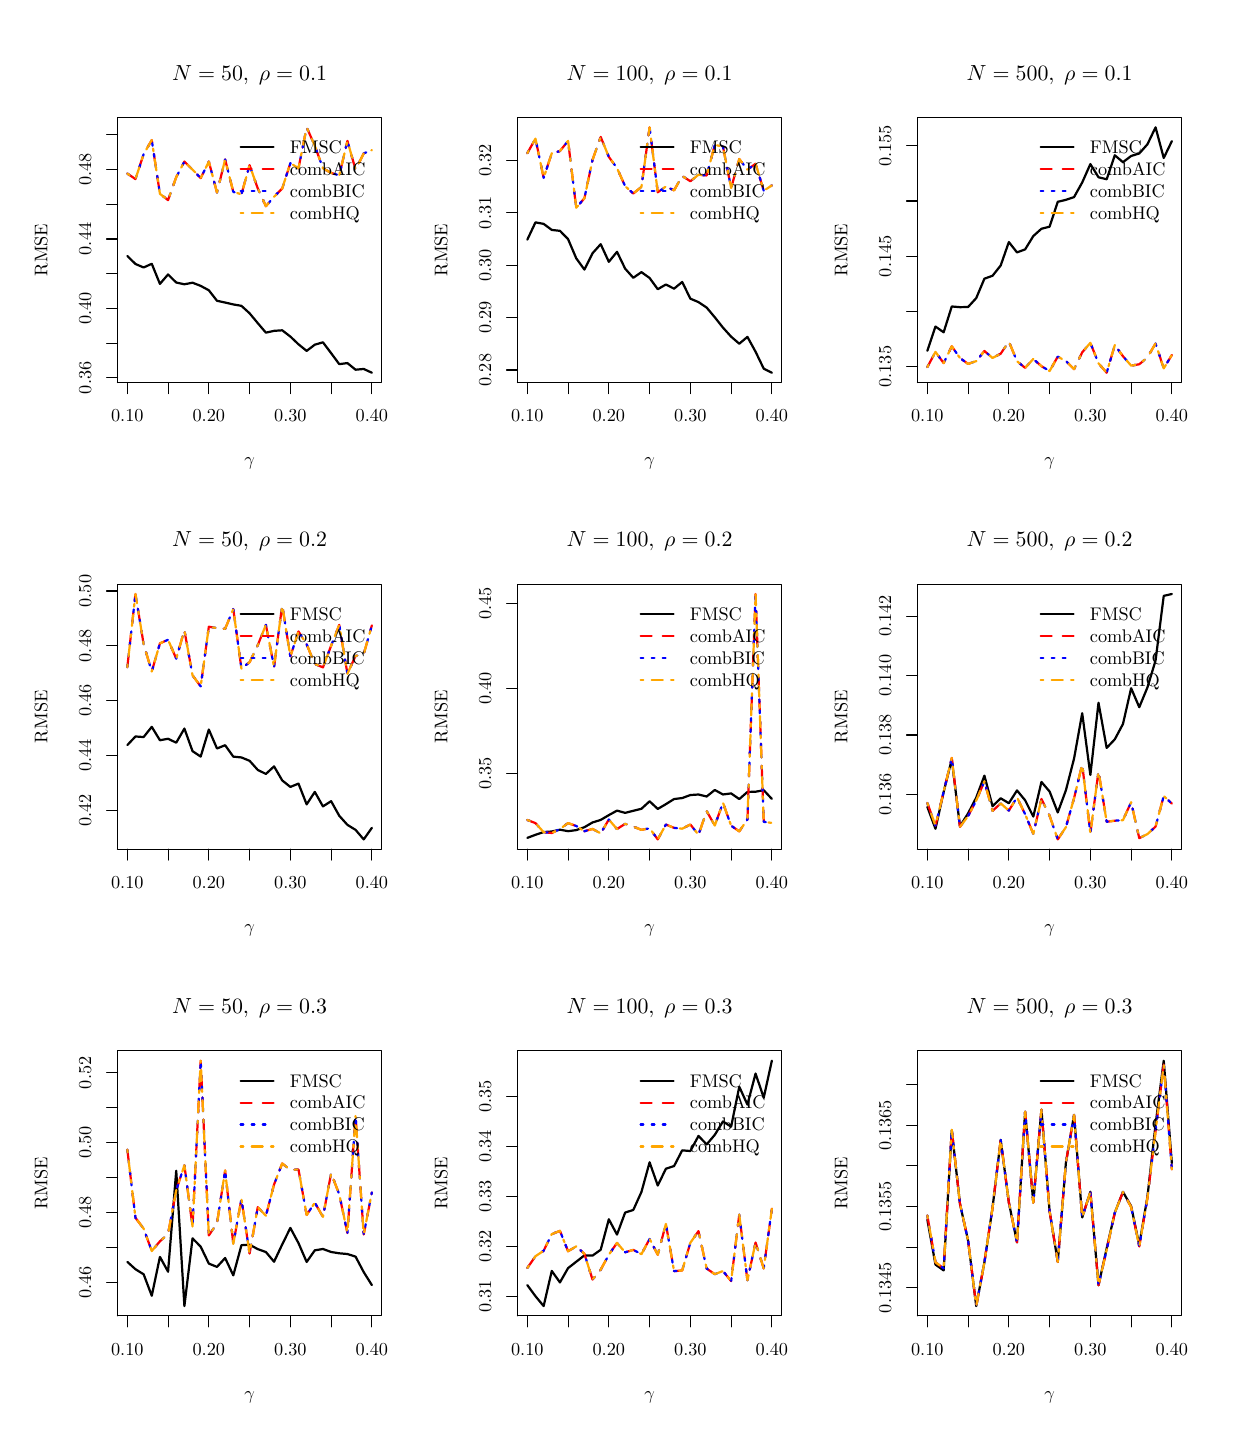
\begin{tikzpicture}[x=1pt,y=1pt]
\definecolor[named]{fillColor}{rgb}{1.00,1.00,1.00}
\path[use as bounding box,fill=fillColor,fill opacity=0.00] (0,0) rectangle (433.62,505.89);
\begin{scope}
\path[clip] ( 32.47,377.65) rectangle (127.91,473.42);
\definecolor[named]{drawColor}{rgb}{0.00,0.00,0.00}

\path[draw=drawColor,line width= 0.8pt,line join=round,line cap=round] ( 36.01,423.38) --
	( 38.95,420.49) --
	( 41.90,419.23) --
	( 44.84,420.56) --
	( 47.79,413.30) --
	( 50.73,416.72) --
	( 53.68,413.79) --
	( 56.63,413.16) --
	( 59.57,413.73) --
	( 62.52,412.58) --
	( 65.46,410.99) --
	( 68.41,407.20) --
	( 71.35,406.56) --
	( 74.30,405.88) --
	( 77.24,405.37) --
	( 80.19,402.67) --
	( 83.14,399.12) --
	( 86.08,395.68) --
	( 89.03,396.33) --
	( 91.97,396.53) --
	( 94.92,394.27) --
	( 97.86,391.47) --
	(100.81,389.09) --
	(103.75,391.33) --
	(106.70,392.19) --
	(109.65,388.27) --
	(112.59,384.30) --
	(115.54,384.69) --
	(118.48,382.29) --
	(121.43,382.56) --
	(124.37,381.20);
\end{scope}
\begin{scope}
\path[clip] (  0.00,  0.00) rectangle (433.62,505.89);
\definecolor[named]{drawColor}{rgb}{0.00,0.00,0.00}

\path[draw=drawColor,line width= 0.4pt,line join=round,line cap=round] ( 36.01,377.65) -- (124.37,377.65);

\path[draw=drawColor,line width= 0.4pt,line join=round,line cap=round] ( 36.01,377.65) -- ( 36.01,373.69);

\path[draw=drawColor,line width= 0.4pt,line join=round,line cap=round] ( 50.73,377.65) -- ( 50.73,373.69);

\path[draw=drawColor,line width= 0.4pt,line join=round,line cap=round] ( 65.46,377.65) -- ( 65.46,373.69);

\path[draw=drawColor,line width= 0.4pt,line join=round,line cap=round] ( 80.19,377.65) -- ( 80.19,373.69);

\path[draw=drawColor,line width= 0.4pt,line join=round,line cap=round] ( 94.92,377.65) -- ( 94.92,373.69);

\path[draw=drawColor,line width= 0.4pt,line join=round,line cap=round] (109.65,377.65) -- (109.65,373.69);

\path[draw=drawColor,line width= 0.4pt,line join=round,line cap=round] (124.37,377.65) -- (124.37,373.69);

\node[text=drawColor,anchor=base,inner sep=0pt, outer sep=0pt, scale=  0.66] at ( 36.01,363.40) {0.10};

\node[text=drawColor,anchor=base,inner sep=0pt, outer sep=0pt, scale=  0.66] at ( 65.46,363.40) {0.20};

\node[text=drawColor,anchor=base,inner sep=0pt, outer sep=0pt, scale=  0.66] at ( 94.92,363.40) {0.30};

\node[text=drawColor,anchor=base,inner sep=0pt, outer sep=0pt, scale=  0.66] at (124.37,363.40) {0.40};

\path[draw=drawColor,line width= 0.4pt,line join=round,line cap=round] ( 32.47,379.34) -- ( 32.47,467.18);

\path[draw=drawColor,line width= 0.4pt,line join=round,line cap=round] ( 32.47,379.34) -- ( 28.51,379.34);

\path[draw=drawColor,line width= 0.4pt,line join=round,line cap=round] ( 32.47,391.89) -- ( 28.51,391.89);

\path[draw=drawColor,line width= 0.4pt,line join=round,line cap=round] ( 32.47,404.44) -- ( 28.51,404.44);

\path[draw=drawColor,line width= 0.4pt,line join=round,line cap=round] ( 32.47,416.99) -- ( 28.51,416.99);

\path[draw=drawColor,line width= 0.4pt,line join=round,line cap=round] ( 32.47,429.54) -- ( 28.51,429.54);

\path[draw=drawColor,line width= 0.4pt,line join=round,line cap=round] ( 32.47,442.08) -- ( 28.51,442.08);

\path[draw=drawColor,line width= 0.4pt,line join=round,line cap=round] ( 32.47,454.63) -- ( 28.51,454.63);

\path[draw=drawColor,line width= 0.4pt,line join=round,line cap=round] ( 32.47,467.18) -- ( 28.51,467.18);

\node[text=drawColor,rotate= 90.00,anchor=base,inner sep=0pt, outer sep=0pt, scale=  0.66] at ( 22.97,379.34) {0.36};

\node[text=drawColor,rotate= 90.00,anchor=base,inner sep=0pt, outer sep=0pt, scale=  0.66] at ( 22.97,404.44) {0.40};

\node[text=drawColor,rotate= 90.00,anchor=base,inner sep=0pt, outer sep=0pt, scale=  0.66] at ( 22.97,429.54) {0.44};

\node[text=drawColor,rotate= 90.00,anchor=base,inner sep=0pt, outer sep=0pt, scale=  0.66] at ( 22.97,454.63) {0.48};

\path[draw=drawColor,line width= 0.4pt,line join=round,line cap=round] ( 32.47,377.65) --
	(127.91,377.65) --
	(127.91,473.42) --
	( 32.47,473.42) --
	( 32.47,377.65);
\end{scope}
\begin{scope}
\path[clip] (  0.00,337.26) rectangle (144.54,505.89);
\definecolor[named]{drawColor}{rgb}{0.00,0.00,0.00}

\node[text=drawColor,anchor=base,inner sep=0pt, outer sep=0pt, scale=  0.79] at ( 80.19,486.92) {\bfseries $N=50, \;\rho=0.1$};

\node[text=drawColor,anchor=base,inner sep=0pt, outer sep=0pt, scale=  0.66] at ( 80.19,347.56) {$\gamma$};

\node[text=drawColor,rotate= 90.00,anchor=base,inner sep=0pt, outer sep=0pt, scale=  0.66] at (  7.13,425.53) {RMSE};
\end{scope}
\begin{scope}
\path[clip] ( 32.47,377.65) rectangle (127.91,473.42);
\definecolor[named]{drawColor}{rgb}{1.00,0.00,0.00}

\path[draw=drawColor,line width= 0.8pt,dash pattern=on 4pt off 4pt ,line join=round,line cap=round] ( 36.01,453.17) --
	( 38.95,451.17) --
	( 41.90,460.17) --
	( 44.84,465.27) --
	( 47.79,445.84) --
	( 50.73,443.57) --
	( 53.68,451.87) --
	( 56.63,457.50) --
	( 59.57,454.60) --
	( 62.52,451.51) --
	( 65.46,457.49) --
	( 68.41,446.28) --
	( 71.35,458.25) --
	( 74.30,446.53) --
	( 77.24,445.68) --
	( 80.19,456.21) --
	( 83.14,447.81) --
	( 86.08,441.36) --
	( 89.03,444.78) --
	( 91.97,447.74) --
	( 94.92,456.93) --
	( 97.86,455.06) --
	(100.81,469.87) --
	(103.75,463.22) --
	(106.70,455.07) --
	(109.65,453.39) --
	(112.59,452.52) --
	(115.54,464.98) --
	(118.48,454.58) --
	(121.43,460.46) --
	(124.37,461.63);
\definecolor[named]{drawColor}{rgb}{0.00,0.00,1.00}

\path[draw=drawColor,line width= 0.8pt,dash pattern=on 1pt off 3pt ,line join=round,line cap=round] ( 36.01,453.17) --
	( 38.95,451.17) --
	( 41.90,460.17) --
	( 44.84,465.27) --
	( 47.79,445.84) --
	( 50.73,443.57) --
	( 53.68,451.87) --
	( 56.63,457.50) --
	( 59.57,454.60) --
	( 62.52,451.51) --
	( 65.46,457.49) --
	( 68.41,446.28) --
	( 71.35,458.25) --
	( 74.30,446.53) --
	( 77.24,445.68) --
	( 80.19,456.21) --
	( 83.14,447.81) --
	( 86.08,441.36) --
	( 89.03,444.78) --
	( 91.97,447.74) --
	( 94.92,456.93) --
	( 97.86,455.06) --
	(100.81,469.87) --
	(103.75,463.22) --
	(106.70,455.07) --
	(109.65,453.39) --
	(112.59,452.52) --
	(115.54,464.98) --
	(118.48,454.58) --
	(121.43,460.46) --
	(124.37,461.63);
\definecolor[named]{drawColor}{rgb}{1.00,0.65,0.00}

\path[draw=drawColor,line width= 0.8pt,dash pattern=on 1pt off 3pt on 4pt off 3pt ,line join=round,line cap=round] ( 36.01,453.17) --
	( 38.95,451.17) --
	( 41.90,460.17) --
	( 44.84,465.27) --
	( 47.79,445.84) --
	( 50.73,443.57) --
	( 53.68,451.87) --
	( 56.63,457.50) --
	( 59.57,454.60) --
	( 62.52,451.51) --
	( 65.46,457.49) --
	( 68.41,446.28) --
	( 71.35,458.25) --
	( 74.30,446.53) --
	( 77.24,445.68) --
	( 80.19,456.21) --
	( 83.14,447.81) --
	( 86.08,441.36) --
	( 89.03,444.78) --
	( 91.97,447.74) --
	( 94.92,456.93) --
	( 97.86,455.06) --
	(100.81,469.87) --
	(103.75,463.22) --
	(106.70,455.07) --
	(109.65,453.39) --
	(112.59,452.52) --
	(115.54,464.98) --
	(118.48,454.58) --
	(121.43,460.46) --
	(124.37,461.63);
\definecolor[named]{drawColor}{rgb}{0.00,0.00,0.00}

\path[draw=drawColor,line width= 0.8pt,line join=round,line cap=round] ( 76.94,462.63) -- ( 88.82,462.63);
\definecolor[named]{drawColor}{rgb}{1.00,0.00,0.00}

\path[draw=drawColor,line width= 0.8pt,dash pattern=on 4pt off 4pt ,line join=round,line cap=round] ( 76.94,454.71) -- ( 88.82,454.71);
\definecolor[named]{drawColor}{rgb}{0.00,0.00,1.00}

\path[draw=drawColor,line width= 0.8pt,dash pattern=on 1pt off 3pt ,line join=round,line cap=round] ( 76.94,446.79) -- ( 88.82,446.79);
\definecolor[named]{drawColor}{rgb}{1.00,0.65,0.00}

\path[draw=drawColor,line width= 0.8pt,dash pattern=on 1pt off 3pt on 4pt off 3pt ,line join=round,line cap=round] ( 76.94,438.87) -- ( 88.82,438.87);
\definecolor[named]{drawColor}{rgb}{0.00,0.00,0.00}

\node[text=drawColor,anchor=base west,inner sep=0pt, outer sep=0pt, scale=  0.66] at ( 94.76,460.35) {FMSC};

\node[text=drawColor,anchor=base west,inner sep=0pt, outer sep=0pt, scale=  0.66] at ( 94.76,452.43) {combAIC};

\node[text=drawColor,anchor=base west,inner sep=0pt, outer sep=0pt, scale=  0.66] at ( 94.76,444.51) {combBIC};

\node[text=drawColor,anchor=base west,inner sep=0pt, outer sep=0pt, scale=  0.66] at ( 94.76,436.59) {combHQ};
\end{scope}
\begin{scope}
\path[clip] (177.01,377.65) rectangle (272.45,473.42);
\definecolor[named]{drawColor}{rgb}{0.00,0.00,0.00}

\path[draw=drawColor,line width= 0.8pt,line join=round,line cap=round] (180.55,429.29) --
	(183.49,435.53) --
	(186.44,434.99) --
	(189.38,432.80) --
	(192.33,432.47) --
	(195.27,429.48) --
	(198.22,422.55) --
	(201.17,418.47) --
	(204.11,424.38) --
	(207.06,427.65) --
	(210.00,421.28) --
	(212.95,424.89) --
	(215.89,418.81) --
	(218.84,415.50) --
	(221.78,417.55) --
	(224.73,415.43) --
	(227.68,411.38) --
	(230.62,413.08) --
	(233.57,411.57) --
	(236.51,414.00) --
	(239.46,407.96) --
	(242.40,406.72) --
	(245.35,404.74) --
	(248.29,401.23) --
	(251.24,397.50) --
	(254.19,394.23) --
	(257.13,391.69) --
	(260.08,394.15) --
	(263.02,388.79) --
	(265.97,382.68) --
	(268.91,381.20);
\end{scope}
\begin{scope}
\path[clip] (  0.00,  0.00) rectangle (433.62,505.89);
\definecolor[named]{drawColor}{rgb}{0.00,0.00,0.00}

\path[draw=drawColor,line width= 0.4pt,line join=round,line cap=round] (180.55,377.65) -- (268.91,377.65);

\path[draw=drawColor,line width= 0.4pt,line join=round,line cap=round] (180.55,377.65) -- (180.55,373.69);

\path[draw=drawColor,line width= 0.4pt,line join=round,line cap=round] (195.27,377.65) -- (195.27,373.69);

\path[draw=drawColor,line width= 0.4pt,line join=round,line cap=round] (210.00,377.65) -- (210.00,373.69);

\path[draw=drawColor,line width= 0.4pt,line join=round,line cap=round] (224.73,377.65) -- (224.73,373.69);

\path[draw=drawColor,line width= 0.4pt,line join=round,line cap=round] (239.46,377.65) -- (239.46,373.69);

\path[draw=drawColor,line width= 0.4pt,line join=round,line cap=round] (254.19,377.65) -- (254.19,373.69);

\path[draw=drawColor,line width= 0.4pt,line join=round,line cap=round] (268.91,377.65) -- (268.91,373.69);

\node[text=drawColor,anchor=base,inner sep=0pt, outer sep=0pt, scale=  0.66] at (180.55,363.40) {0.10};

\node[text=drawColor,anchor=base,inner sep=0pt, outer sep=0pt, scale=  0.66] at (210.00,363.40) {0.20};

\node[text=drawColor,anchor=base,inner sep=0pt, outer sep=0pt, scale=  0.66] at (239.46,363.40) {0.30};

\node[text=drawColor,anchor=base,inner sep=0pt, outer sep=0pt, scale=  0.66] at (268.91,363.40) {0.40};

\path[draw=drawColor,line width= 0.4pt,line join=round,line cap=round] (177.01,382.17) -- (177.01,457.92);

\path[draw=drawColor,line width= 0.4pt,line join=round,line cap=round] (177.01,382.17) -- (173.05,382.17);

\path[draw=drawColor,line width= 0.4pt,line join=round,line cap=round] (177.01,401.11) -- (173.05,401.11);

\path[draw=drawColor,line width= 0.4pt,line join=round,line cap=round] (177.01,420.04) -- (173.05,420.04);

\path[draw=drawColor,line width= 0.4pt,line join=round,line cap=round] (177.01,438.98) -- (173.05,438.98);

\path[draw=drawColor,line width= 0.4pt,line join=round,line cap=round] (177.01,457.92) -- (173.05,457.92);

\node[text=drawColor,rotate= 90.00,anchor=base,inner sep=0pt, outer sep=0pt, scale=  0.66] at (167.51,382.17) {0.28};

\node[text=drawColor,rotate= 90.00,anchor=base,inner sep=0pt, outer sep=0pt, scale=  0.66] at (167.51,401.11) {0.29};

\node[text=drawColor,rotate= 90.00,anchor=base,inner sep=0pt, outer sep=0pt, scale=  0.66] at (167.51,420.04) {0.30};

\node[text=drawColor,rotate= 90.00,anchor=base,inner sep=0pt, outer sep=0pt, scale=  0.66] at (167.51,438.98) {0.31};

\node[text=drawColor,rotate= 90.00,anchor=base,inner sep=0pt, outer sep=0pt, scale=  0.66] at (167.51,457.92) {0.32};

\path[draw=drawColor,line width= 0.4pt,line join=round,line cap=round] (177.01,377.65) --
	(272.45,377.65) --
	(272.45,473.42) --
	(177.01,473.42) --
	(177.01,377.65);
\end{scope}
\begin{scope}
\path[clip] (144.54,337.26) rectangle (289.08,505.89);
\definecolor[named]{drawColor}{rgb}{0.00,0.00,0.00}

\node[text=drawColor,anchor=base,inner sep=0pt, outer sep=0pt, scale=  0.79] at (224.73,486.92) {\bfseries $N=100, \;\rho=0.1$};

\node[text=drawColor,anchor=base,inner sep=0pt, outer sep=0pt, scale=  0.66] at (224.73,347.56) {$\gamma$};

\node[text=drawColor,rotate= 90.00,anchor=base,inner sep=0pt, outer sep=0pt, scale=  0.66] at (151.67,425.53) {RMSE};
\end{scope}
\begin{scope}
\path[clip] (177.01,377.65) rectangle (272.45,473.42);
\definecolor[named]{drawColor}{rgb}{1.00,0.00,0.00}

\path[draw=drawColor,line width= 0.8pt,dash pattern=on 4pt off 4pt ,line join=round,line cap=round] (180.55,460.52) --
	(183.49,465.80) --
	(186.44,451.60) --
	(189.38,460.47) --
	(192.33,461.28) --
	(195.27,464.98) --
	(198.22,440.82) --
	(201.17,444.23) --
	(204.11,458.12) --
	(207.06,466.40) --
	(210.00,459.19) --
	(212.95,455.15) --
	(215.89,448.61) --
	(218.84,445.97) --
	(221.78,448.34) --
	(224.73,469.87) --
	(227.68,446.39) --
	(230.62,448.51) --
	(233.57,447.09) --
	(236.51,452.31) --
	(239.46,450.38) --
	(242.40,452.75) --
	(245.35,452.47) --
	(248.29,463.54) --
	(251.24,462.90) --
	(254.19,447.95) --
	(257.13,458.43) --
	(260.08,454.57) --
	(263.02,456.71) --
	(265.97,446.97) --
	(268.91,448.88);
\definecolor[named]{drawColor}{rgb}{0.00,0.00,1.00}

\path[draw=drawColor,line width= 0.8pt,dash pattern=on 1pt off 3pt ,line join=round,line cap=round] (180.55,460.52) --
	(183.49,465.80) --
	(186.44,451.60) --
	(189.38,460.47) --
	(192.33,461.28) --
	(195.27,464.98) --
	(198.22,440.82) --
	(201.17,444.23) --
	(204.11,458.12) --
	(207.06,466.40) --
	(210.00,459.19) --
	(212.95,455.15) --
	(215.89,448.61) --
	(218.84,445.97) --
	(221.78,448.34) --
	(224.73,469.87) --
	(227.68,446.39) --
	(230.62,448.51) --
	(233.57,447.09) --
	(236.51,452.31) --
	(239.46,450.38) --
	(242.40,452.75) --
	(245.35,452.47) --
	(248.29,463.54) --
	(251.24,462.90) --
	(254.19,447.95) --
	(257.13,458.43) --
	(260.08,454.57) --
	(263.02,456.71) --
	(265.97,446.97) --
	(268.91,448.88);
\definecolor[named]{drawColor}{rgb}{1.00,0.65,0.00}

\path[draw=drawColor,line width= 0.8pt,dash pattern=on 1pt off 3pt on 4pt off 3pt ,line join=round,line cap=round] (180.55,460.52) --
	(183.49,465.80) --
	(186.44,451.60) --
	(189.38,460.47) --
	(192.33,461.28) --
	(195.27,464.98) --
	(198.22,440.82) --
	(201.17,444.23) --
	(204.11,458.12) --
	(207.06,466.40) --
	(210.00,459.19) --
	(212.95,455.15) --
	(215.89,448.61) --
	(218.84,445.97) --
	(221.78,448.34) --
	(224.73,469.87) --
	(227.68,446.39) --
	(230.62,448.51) --
	(233.57,447.09) --
	(236.51,452.31) --
	(239.46,450.38) --
	(242.40,452.75) --
	(245.35,452.47) --
	(248.29,463.54) --
	(251.24,462.90) --
	(254.19,447.95) --
	(257.13,458.43) --
	(260.08,454.57) --
	(263.02,456.71) --
	(265.97,446.97) --
	(268.91,448.88);
\definecolor[named]{drawColor}{rgb}{0.00,0.00,0.00}

\path[draw=drawColor,line width= 0.8pt,line join=round,line cap=round] (221.48,462.63) -- (233.36,462.63);
\definecolor[named]{drawColor}{rgb}{1.00,0.00,0.00}

\path[draw=drawColor,line width= 0.8pt,dash pattern=on 4pt off 4pt ,line join=round,line cap=round] (221.48,454.71) -- (233.36,454.71);
\definecolor[named]{drawColor}{rgb}{0.00,0.00,1.00}

\path[draw=drawColor,line width= 0.8pt,dash pattern=on 1pt off 3pt ,line join=round,line cap=round] (221.48,446.79) -- (233.36,446.79);
\definecolor[named]{drawColor}{rgb}{1.00,0.65,0.00}

\path[draw=drawColor,line width= 0.8pt,dash pattern=on 1pt off 3pt on 4pt off 3pt ,line join=round,line cap=round] (221.48,438.87) -- (233.36,438.87);
\definecolor[named]{drawColor}{rgb}{0.00,0.00,0.00}

\node[text=drawColor,anchor=base west,inner sep=0pt, outer sep=0pt, scale=  0.66] at (239.30,460.35) {FMSC};

\node[text=drawColor,anchor=base west,inner sep=0pt, outer sep=0pt, scale=  0.66] at (239.30,452.43) {combAIC};

\node[text=drawColor,anchor=base west,inner sep=0pt, outer sep=0pt, scale=  0.66] at (239.30,444.51) {combBIC};

\node[text=drawColor,anchor=base west,inner sep=0pt, outer sep=0pt, scale=  0.66] at (239.30,436.59) {combHQ};
\end{scope}
\begin{scope}
\path[clip] (321.55,377.65) rectangle (416.99,473.42);
\definecolor[named]{drawColor}{rgb}{0.00,0.00,0.00}

\path[draw=drawColor,line width= 0.8pt,line join=round,line cap=round] (325.09,389.15) --
	(328.03,397.89) --
	(330.98,395.81) --
	(333.92,405.14) --
	(336.87,404.89) --
	(339.81,404.94) --
	(342.76,408.17) --
	(345.71,415.18) --
	(348.65,416.24) --
	(351.60,419.96) --
	(354.54,428.42) --
	(357.49,424.68) --
	(360.43,425.77) --
	(363.38,430.58) --
	(366.32,433.22) --
	(369.27,433.98) --
	(372.22,442.96) --
	(375.16,443.67) --
	(378.11,444.67) --
	(381.05,449.95) --
	(384.00,456.60) --
	(386.94,451.83) --
	(389.89,451.11) --
	(392.83,459.77) --
	(395.78,457.28) --
	(398.73,459.52) --
	(401.67,460.43) --
	(404.62,463.74) --
	(407.56,469.87) --
	(410.51,458.80) --
	(413.45,464.89);
\end{scope}
\begin{scope}
\path[clip] (  0.00,  0.00) rectangle (433.62,505.89);
\definecolor[named]{drawColor}{rgb}{0.00,0.00,0.00}

\path[draw=drawColor,line width= 0.4pt,line join=round,line cap=round] (325.09,377.65) -- (413.45,377.65);

\path[draw=drawColor,line width= 0.4pt,line join=round,line cap=round] (325.09,377.65) -- (325.09,373.69);

\path[draw=drawColor,line width= 0.4pt,line join=round,line cap=round] (339.81,377.65) -- (339.81,373.69);

\path[draw=drawColor,line width= 0.4pt,line join=round,line cap=round] (354.54,377.65) -- (354.54,373.69);

\path[draw=drawColor,line width= 0.4pt,line join=round,line cap=round] (369.27,377.65) -- (369.27,373.69);

\path[draw=drawColor,line width= 0.4pt,line join=round,line cap=round] (384.00,377.65) -- (384.00,373.69);

\path[draw=drawColor,line width= 0.4pt,line join=round,line cap=round] (398.73,377.65) -- (398.73,373.69);

\path[draw=drawColor,line width= 0.4pt,line join=round,line cap=round] (413.45,377.65) -- (413.45,373.69);

\node[text=drawColor,anchor=base,inner sep=0pt, outer sep=0pt, scale=  0.66] at (325.09,363.40) {0.10};

\node[text=drawColor,anchor=base,inner sep=0pt, outer sep=0pt, scale=  0.66] at (354.54,363.40) {0.20};

\node[text=drawColor,anchor=base,inner sep=0pt, outer sep=0pt, scale=  0.66] at (384.00,363.40) {0.30};

\node[text=drawColor,anchor=base,inner sep=0pt, outer sep=0pt, scale=  0.66] at (413.45,363.40) {0.40};

\path[draw=drawColor,line width= 0.4pt,line join=round,line cap=round] (321.55,383.40) -- (321.55,463.20);

\path[draw=drawColor,line width= 0.4pt,line join=round,line cap=round] (321.55,383.40) -- (317.59,383.40);

\path[draw=drawColor,line width= 0.4pt,line join=round,line cap=round] (321.55,403.35) -- (317.59,403.35);

\path[draw=drawColor,line width= 0.4pt,line join=round,line cap=round] (321.55,423.30) -- (317.59,423.30);

\path[draw=drawColor,line width= 0.4pt,line join=round,line cap=round] (321.55,443.25) -- (317.59,443.25);

\path[draw=drawColor,line width= 0.4pt,line join=round,line cap=round] (321.55,463.20) -- (317.59,463.20);

\node[text=drawColor,rotate= 90.00,anchor=base,inner sep=0pt, outer sep=0pt, scale=  0.66] at (312.05,383.40) {0.135};

\node[text=drawColor,rotate= 90.00,anchor=base,inner sep=0pt, outer sep=0pt, scale=  0.66] at (312.05,423.30) {0.145};

\node[text=drawColor,rotate= 90.00,anchor=base,inner sep=0pt, outer sep=0pt, scale=  0.66] at (312.05,463.20) {0.155};

\path[draw=drawColor,line width= 0.4pt,line join=round,line cap=round] (321.55,377.65) --
	(416.99,377.65) --
	(416.99,473.42) --
	(321.55,473.42) --
	(321.55,377.65);
\end{scope}
\begin{scope}
\path[clip] (289.08,337.26) rectangle (433.62,505.89);
\definecolor[named]{drawColor}{rgb}{0.00,0.00,0.00}

\node[text=drawColor,anchor=base,inner sep=0pt, outer sep=0pt, scale=  0.79] at (369.27,486.92) {\bfseries $N=500, \;\rho=0.1$};

\node[text=drawColor,anchor=base,inner sep=0pt, outer sep=0pt, scale=  0.66] at (369.27,347.56) {$\gamma$};

\node[text=drawColor,rotate= 90.00,anchor=base,inner sep=0pt, outer sep=0pt, scale=  0.66] at (296.21,425.53) {RMSE};
\end{scope}
\begin{scope}
\path[clip] (321.55,377.65) rectangle (416.99,473.42);
\definecolor[named]{drawColor}{rgb}{1.00,0.00,0.00}

\path[draw=drawColor,line width= 0.8pt,dash pattern=on 4pt off 4pt ,line join=round,line cap=round] (325.09,383.23) --
	(328.03,388.73) --
	(330.98,384.68) --
	(333.92,390.75) --
	(336.87,386.53) --
	(339.81,384.38) --
	(342.76,385.40) --
	(345.71,389.05) --
	(348.65,386.53) --
	(351.60,388.08) --
	(354.54,392.48) --
	(357.49,385.37) --
	(360.43,382.95) --
	(363.38,386.17) --
	(366.32,383.56) --
	(369.27,381.82) --
	(372.22,387.02) --
	(375.16,385.41) --
	(378.11,382.49) --
	(381.05,388.57) --
	(384.00,392.00) --
	(386.94,384.61) --
	(389.89,381.20) --
	(392.83,391.18) --
	(395.78,387.16) --
	(398.73,383.77) --
	(401.67,384.25) --
	(404.62,386.74) --
	(407.56,391.77) --
	(410.51,382.78) --
	(413.45,387.62);
\definecolor[named]{drawColor}{rgb}{0.00,0.00,1.00}

\path[draw=drawColor,line width= 0.8pt,dash pattern=on 1pt off 3pt ,line join=round,line cap=round] (325.09,383.23) --
	(328.03,388.73) --
	(330.98,384.68) --
	(333.92,390.75) --
	(336.87,386.53) --
	(339.81,384.38) --
	(342.76,385.40) --
	(345.71,389.05) --
	(348.65,386.53) --
	(351.60,388.08) --
	(354.54,392.48) --
	(357.49,385.37) --
	(360.43,382.95) --
	(363.38,386.17) --
	(366.32,383.56) --
	(369.27,381.82) --
	(372.22,387.02) --
	(375.16,385.41) --
	(378.11,382.49) --
	(381.05,388.57) --
	(384.00,392.00) --
	(386.94,384.61) --
	(389.89,381.20) --
	(392.83,391.18) --
	(395.78,387.16) --
	(398.73,383.77) --
	(401.67,384.25) --
	(404.62,386.74) --
	(407.56,391.77) --
	(410.51,382.78) --
	(413.45,387.62);
\definecolor[named]{drawColor}{rgb}{1.00,0.65,0.00}

\path[draw=drawColor,line width= 0.8pt,dash pattern=on 1pt off 3pt on 4pt off 3pt ,line join=round,line cap=round] (325.09,383.23) --
	(328.03,388.73) --
	(330.98,384.68) --
	(333.92,390.75) --
	(336.87,386.53) --
	(339.81,384.38) --
	(342.76,385.40) --
	(345.71,389.05) --
	(348.65,386.53) --
	(351.60,388.08) --
	(354.54,392.48) --
	(357.49,385.37) --
	(360.43,382.95) --
	(363.38,386.17) --
	(366.32,383.56) --
	(369.27,381.82) --
	(372.22,387.02) --
	(375.16,385.41) --
	(378.11,382.49) --
	(381.05,388.57) --
	(384.00,392.00) --
	(386.94,384.61) --
	(389.89,381.20) --
	(392.83,391.18) --
	(395.78,387.16) --
	(398.73,383.77) --
	(401.67,384.25) --
	(404.62,386.74) --
	(407.56,391.77) --
	(410.51,382.78) --
	(413.45,387.62);
\definecolor[named]{drawColor}{rgb}{0.00,0.00,0.00}

\path[draw=drawColor,line width= 0.8pt,line join=round,line cap=round] (366.02,462.63) -- (377.90,462.63);
\definecolor[named]{drawColor}{rgb}{1.00,0.00,0.00}

\path[draw=drawColor,line width= 0.8pt,dash pattern=on 4pt off 4pt ,line join=round,line cap=round] (366.02,454.71) -- (377.90,454.71);
\definecolor[named]{drawColor}{rgb}{0.00,0.00,1.00}

\path[draw=drawColor,line width= 0.8pt,dash pattern=on 1pt off 3pt ,line join=round,line cap=round] (366.02,446.79) -- (377.90,446.79);
\definecolor[named]{drawColor}{rgb}{1.00,0.65,0.00}

\path[draw=drawColor,line width= 0.8pt,dash pattern=on 1pt off 3pt on 4pt off 3pt ,line join=round,line cap=round] (366.02,438.87) -- (377.90,438.87);
\definecolor[named]{drawColor}{rgb}{0.00,0.00,0.00}

\node[text=drawColor,anchor=base west,inner sep=0pt, outer sep=0pt, scale=  0.66] at (383.84,460.35) {FMSC};

\node[text=drawColor,anchor=base west,inner sep=0pt, outer sep=0pt, scale=  0.66] at (383.84,452.43) {combAIC};

\node[text=drawColor,anchor=base west,inner sep=0pt, outer sep=0pt, scale=  0.66] at (383.84,444.51) {combBIC};

\node[text=drawColor,anchor=base west,inner sep=0pt, outer sep=0pt, scale=  0.66] at (383.84,436.59) {combHQ};
\end{scope}
\begin{scope}
\path[clip] ( 32.47,209.02) rectangle (127.91,304.79);
\definecolor[named]{drawColor}{rgb}{0.00,0.00,0.00}

\path[draw=drawColor,line width= 0.8pt,line join=round,line cap=round] ( 36.01,246.65) --
	( 38.95,249.76) --
	( 41.90,249.55) --
	( 44.84,253.24) --
	( 47.79,248.40) --
	( 50.73,248.93) --
	( 53.68,247.52) --
	( 56.63,252.61) --
	( 59.57,244.46) --
	( 62.52,242.50) --
	( 65.46,252.27) --
	( 68.41,245.42) --
	( 71.35,246.60) --
	( 74.30,242.48) --
	( 77.24,242.18) --
	( 80.19,240.97) --
	( 83.14,237.68) --
	( 86.08,236.22) --
	( 89.03,238.96) --
	( 91.97,233.89) --
	( 94.92,231.53) --
	( 97.86,232.73) --
	(100.81,225.22) --
	(103.75,229.73) --
	(106.70,224.50) --
	(109.65,226.38) --
	(112.59,221.10) --
	(115.54,217.82) --
	(118.48,216.02) --
	(121.43,212.57) --
	(124.37,216.74);
\end{scope}
\begin{scope}
\path[clip] (  0.00,  0.00) rectangle (433.62,505.89);
\definecolor[named]{drawColor}{rgb}{0.00,0.00,0.00}

\path[draw=drawColor,line width= 0.4pt,line join=round,line cap=round] ( 36.01,209.02) -- (124.37,209.02);

\path[draw=drawColor,line width= 0.4pt,line join=round,line cap=round] ( 36.01,209.02) -- ( 36.01,205.06);

\path[draw=drawColor,line width= 0.4pt,line join=round,line cap=round] ( 50.73,209.02) -- ( 50.73,205.06);

\path[draw=drawColor,line width= 0.4pt,line join=round,line cap=round] ( 65.46,209.02) -- ( 65.46,205.06);

\path[draw=drawColor,line width= 0.4pt,line join=round,line cap=round] ( 80.19,209.02) -- ( 80.19,205.06);

\path[draw=drawColor,line width= 0.4pt,line join=round,line cap=round] ( 94.92,209.02) -- ( 94.92,205.06);

\path[draw=drawColor,line width= 0.4pt,line join=round,line cap=round] (109.65,209.02) -- (109.65,205.06);

\path[draw=drawColor,line width= 0.4pt,line join=round,line cap=round] (124.37,209.02) -- (124.37,205.06);

\node[text=drawColor,anchor=base,inner sep=0pt, outer sep=0pt, scale=  0.66] at ( 36.01,194.77) {0.10};

\node[text=drawColor,anchor=base,inner sep=0pt, outer sep=0pt, scale=  0.66] at ( 65.46,194.77) {0.20};

\node[text=drawColor,anchor=base,inner sep=0pt, outer sep=0pt, scale=  0.66] at ( 94.92,194.77) {0.30};

\node[text=drawColor,anchor=base,inner sep=0pt, outer sep=0pt, scale=  0.66] at (124.37,194.77) {0.40};

\path[draw=drawColor,line width= 0.4pt,line join=round,line cap=round] ( 32.47,223.06) -- ( 32.47,302.31);

\path[draw=drawColor,line width= 0.4pt,line join=round,line cap=round] ( 32.47,223.06) -- ( 28.51,223.06);

\path[draw=drawColor,line width= 0.4pt,line join=round,line cap=round] ( 32.47,242.87) -- ( 28.51,242.87);

\path[draw=drawColor,line width= 0.4pt,line join=round,line cap=round] ( 32.47,262.68) -- ( 28.51,262.68);

\path[draw=drawColor,line width= 0.4pt,line join=round,line cap=round] ( 32.47,282.49) -- ( 28.51,282.49);

\path[draw=drawColor,line width= 0.4pt,line join=round,line cap=round] ( 32.47,302.31) -- ( 28.51,302.31);

\node[text=drawColor,rotate= 90.00,anchor=base,inner sep=0pt, outer sep=0pt, scale=  0.66] at ( 22.97,223.06) {0.42};

\node[text=drawColor,rotate= 90.00,anchor=base,inner sep=0pt, outer sep=0pt, scale=  0.66] at ( 22.97,242.87) {0.44};

\node[text=drawColor,rotate= 90.00,anchor=base,inner sep=0pt, outer sep=0pt, scale=  0.66] at ( 22.97,262.68) {0.46};

\node[text=drawColor,rotate= 90.00,anchor=base,inner sep=0pt, outer sep=0pt, scale=  0.66] at ( 22.97,282.49) {0.48};

\node[text=drawColor,rotate= 90.00,anchor=base,inner sep=0pt, outer sep=0pt, scale=  0.66] at ( 22.97,302.31) {0.50};

\path[draw=drawColor,line width= 0.4pt,line join=round,line cap=round] ( 32.47,209.02) --
	(127.91,209.02) --
	(127.91,304.79) --
	( 32.47,304.79) --
	( 32.47,209.02);
\end{scope}
\begin{scope}
\path[clip] (  0.00,168.63) rectangle (144.54,337.26);
\definecolor[named]{drawColor}{rgb}{0.00,0.00,0.00}

\node[text=drawColor,anchor=base,inner sep=0pt, outer sep=0pt, scale=  0.79] at ( 80.19,318.29) {\bfseries $N=50, \;\rho=0.2$};

\node[text=drawColor,anchor=base,inner sep=0pt, outer sep=0pt, scale=  0.66] at ( 80.19,178.93) {$\gamma$};

\node[text=drawColor,rotate= 90.00,anchor=base,inner sep=0pt, outer sep=0pt, scale=  0.66] at (  7.13,256.90) {RMSE};
\end{scope}
\begin{scope}
\path[clip] ( 32.47,209.02) rectangle (127.91,304.79);
\definecolor[named]{drawColor}{rgb}{1.00,0.00,0.00}

\path[draw=drawColor,line width= 0.8pt,dash pattern=on 4pt off 4pt ,line join=round,line cap=round] ( 36.01,274.80) --
	( 38.95,301.24) --
	( 41.90,283.11) --
	( 44.84,273.23) --
	( 47.79,283.41) --
	( 50.73,284.71) --
	( 53.68,277.87) --
	( 56.63,288.17) --
	( 59.57,271.86) --
	( 62.52,267.85) --
	( 65.46,289.41) --
	( 68.41,288.94) --
	( 71.35,288.66) --
	( 74.30,295.80) --
	( 77.24,274.30) --
	( 80.19,276.62) --
	( 83.14,282.73) --
	( 86.08,290.09) --
	( 89.03,274.92) --
	( 91.97,297.20) --
	( 94.92,278.71) --
	( 97.86,287.71) --
	(100.81,283.03) --
	(103.75,275.98) --
	(106.70,274.72) --
	(109.65,282.55) --
	(112.59,290.08) --
	(115.54,272.42) --
	(118.48,278.88) --
	(121.43,279.53) --
	(124.37,289.90);
\definecolor[named]{drawColor}{rgb}{0.00,0.00,1.00}

\path[draw=drawColor,line width= 0.8pt,dash pattern=on 1pt off 3pt ,line join=round,line cap=round] ( 36.01,274.80) --
	( 38.95,301.24) --
	( 41.90,283.11) --
	( 44.84,273.23) --
	( 47.79,283.41) --
	( 50.73,284.71) --
	( 53.68,277.87) --
	( 56.63,288.17) --
	( 59.57,271.86) --
	( 62.52,267.85) --
	( 65.46,289.41) --
	( 68.41,288.94) --
	( 71.35,288.66) --
	( 74.30,295.80) --
	( 77.24,274.30) --
	( 80.19,276.62) --
	( 83.14,282.73) --
	( 86.08,290.09) --
	( 89.03,274.92) --
	( 91.97,297.20) --
	( 94.92,278.71) --
	( 97.86,287.71) --
	(100.81,283.03) --
	(103.75,275.98) --
	(106.70,274.72) --
	(109.65,282.55) --
	(112.59,290.08) --
	(115.54,272.42) --
	(118.48,278.88) --
	(121.43,279.53) --
	(124.37,289.90);
\definecolor[named]{drawColor}{rgb}{1.00,0.65,0.00}

\path[draw=drawColor,line width= 0.8pt,dash pattern=on 1pt off 3pt on 4pt off 3pt ,line join=round,line cap=round] ( 36.01,274.80) --
	( 38.95,301.24) --
	( 41.90,283.11) --
	( 44.84,273.23) --
	( 47.79,283.41) --
	( 50.73,284.71) --
	( 53.68,277.87) --
	( 56.63,288.17) --
	( 59.57,271.86) --
	( 62.52,267.85) --
	( 65.46,289.41) --
	( 68.41,288.94) --
	( 71.35,288.66) --
	( 74.30,295.80) --
	( 77.24,274.30) --
	( 80.19,276.62) --
	( 83.14,282.73) --
	( 86.08,290.09) --
	( 89.03,274.92) --
	( 91.97,297.20) --
	( 94.92,278.71) --
	( 97.86,287.71) --
	(100.81,283.03) --
	(103.75,275.98) --
	(106.70,274.72) --
	(109.65,282.55) --
	(112.59,290.08) --
	(115.54,272.42) --
	(118.48,278.88) --
	(121.43,279.53) --
	(124.37,289.90);
\definecolor[named]{drawColor}{rgb}{0.00,0.00,0.00}

\path[draw=drawColor,line width= 0.8pt,line join=round,line cap=round] ( 76.94,294.00) -- ( 88.82,294.00);
\definecolor[named]{drawColor}{rgb}{1.00,0.00,0.00}

\path[draw=drawColor,line width= 0.8pt,dash pattern=on 4pt off 4pt ,line join=round,line cap=round] ( 76.94,286.08) -- ( 88.82,286.08);
\definecolor[named]{drawColor}{rgb}{0.00,0.00,1.00}

\path[draw=drawColor,line width= 0.8pt,dash pattern=on 1pt off 3pt ,line join=round,line cap=round] ( 76.94,278.16) -- ( 88.82,278.16);
\definecolor[named]{drawColor}{rgb}{1.00,0.65,0.00}

\path[draw=drawColor,line width= 0.8pt,dash pattern=on 1pt off 3pt on 4pt off 3pt ,line join=round,line cap=round] ( 76.94,270.24) -- ( 88.82,270.24);
\definecolor[named]{drawColor}{rgb}{0.00,0.00,0.00}

\node[text=drawColor,anchor=base west,inner sep=0pt, outer sep=0pt, scale=  0.66] at ( 94.76,291.72) {FMSC};

\node[text=drawColor,anchor=base west,inner sep=0pt, outer sep=0pt, scale=  0.66] at ( 94.76,283.80) {combAIC};

\node[text=drawColor,anchor=base west,inner sep=0pt, outer sep=0pt, scale=  0.66] at ( 94.76,275.88) {combBIC};

\node[text=drawColor,anchor=base west,inner sep=0pt, outer sep=0pt, scale=  0.66] at ( 94.76,267.96) {combHQ};
\end{scope}
\begin{scope}
\path[clip] (177.01,209.02) rectangle (272.45,304.79);
\definecolor[named]{drawColor}{rgb}{0.00,0.00,0.00}

\path[draw=drawColor,line width= 0.8pt,line join=round,line cap=round] (180.55,213.12) --
	(183.49,214.23) --
	(186.44,215.23) --
	(189.38,215.42) --
	(192.33,216.08) --
	(195.27,215.54) --
	(198.22,215.92) --
	(201.17,216.98) --
	(204.11,218.69) --
	(207.06,219.61) --
	(210.00,221.34) --
	(212.95,222.97) --
	(215.89,222.16) --
	(218.84,222.90) --
	(221.78,223.64) --
	(224.73,226.34) --
	(227.68,223.58) --
	(230.62,225.31) --
	(233.57,227.15) --
	(236.51,227.51) --
	(239.46,228.60) --
	(242.40,228.79) --
	(245.35,228.07) --
	(248.29,230.43) --
	(251.24,228.80) --
	(254.19,229.19) --
	(257.13,227.14) --
	(260.08,229.71) --
	(263.02,229.80) --
	(265.97,230.34) --
	(268.91,227.19);
\end{scope}
\begin{scope}
\path[clip] (  0.00,  0.00) rectangle (433.62,505.89);
\definecolor[named]{drawColor}{rgb}{0.00,0.00,0.00}

\path[draw=drawColor,line width= 0.4pt,line join=round,line cap=round] (180.55,209.02) -- (268.91,209.02);

\path[draw=drawColor,line width= 0.4pt,line join=round,line cap=round] (180.55,209.02) -- (180.55,205.06);

\path[draw=drawColor,line width= 0.4pt,line join=round,line cap=round] (195.27,209.02) -- (195.27,205.06);

\path[draw=drawColor,line width= 0.4pt,line join=round,line cap=round] (210.00,209.02) -- (210.00,205.06);

\path[draw=drawColor,line width= 0.4pt,line join=round,line cap=round] (224.73,209.02) -- (224.73,205.06);

\path[draw=drawColor,line width= 0.4pt,line join=round,line cap=round] (239.46,209.02) -- (239.46,205.06);

\path[draw=drawColor,line width= 0.4pt,line join=round,line cap=round] (254.19,209.02) -- (254.19,205.06);

\path[draw=drawColor,line width= 0.4pt,line join=round,line cap=round] (268.91,209.02) -- (268.91,205.06);

\node[text=drawColor,anchor=base,inner sep=0pt, outer sep=0pt, scale=  0.66] at (180.55,194.77) {0.10};

\node[text=drawColor,anchor=base,inner sep=0pt, outer sep=0pt, scale=  0.66] at (210.00,194.77) {0.20};

\node[text=drawColor,anchor=base,inner sep=0pt, outer sep=0pt, scale=  0.66] at (239.46,194.77) {0.30};

\node[text=drawColor,anchor=base,inner sep=0pt, outer sep=0pt, scale=  0.66] at (268.91,194.77) {0.40};

\path[draw=drawColor,line width= 0.4pt,line join=round,line cap=round] (177.01,236.38) -- (177.01,297.75);

\path[draw=drawColor,line width= 0.4pt,line join=round,line cap=round] (177.01,236.38) -- (173.05,236.38);

\path[draw=drawColor,line width= 0.4pt,line join=round,line cap=round] (177.01,267.07) -- (173.05,267.07);

\path[draw=drawColor,line width= 0.4pt,line join=round,line cap=round] (177.01,297.75) -- (173.05,297.75);

\node[text=drawColor,rotate= 90.00,anchor=base,inner sep=0pt, outer sep=0pt, scale=  0.66] at (167.51,236.38) {0.35};

\node[text=drawColor,rotate= 90.00,anchor=base,inner sep=0pt, outer sep=0pt, scale=  0.66] at (167.51,267.07) {0.40};

\node[text=drawColor,rotate= 90.00,anchor=base,inner sep=0pt, outer sep=0pt, scale=  0.66] at (167.51,297.75) {0.45};

\path[draw=drawColor,line width= 0.4pt,line join=round,line cap=round] (177.01,209.02) --
	(272.45,209.02) --
	(272.45,304.79) --
	(177.01,304.79) --
	(177.01,209.02);
\end{scope}
\begin{scope}
\path[clip] (144.54,168.63) rectangle (289.08,337.26);
\definecolor[named]{drawColor}{rgb}{0.00,0.00,0.00}

\node[text=drawColor,anchor=base,inner sep=0pt, outer sep=0pt, scale=  0.79] at (224.73,318.29) {\bfseries $N=100, \;\rho=0.2$};

\node[text=drawColor,anchor=base,inner sep=0pt, outer sep=0pt, scale=  0.66] at (224.73,178.93) {$\gamma$};

\node[text=drawColor,rotate= 90.00,anchor=base,inner sep=0pt, outer sep=0pt, scale=  0.66] at (151.67,256.90) {RMSE};
\end{scope}
\begin{scope}
\path[clip] (177.01,209.02) rectangle (272.45,304.79);
\definecolor[named]{drawColor}{rgb}{1.00,0.00,0.00}

\path[draw=drawColor,line width= 0.8pt,dash pattern=on 4pt off 4pt ,line join=round,line cap=round] (180.55,219.60) --
	(183.49,218.45) --
	(186.44,215.18) --
	(189.38,214.88) --
	(192.33,216.33) --
	(195.27,218.46) --
	(198.22,217.42) --
	(201.17,215.52) --
	(204.11,216.34) --
	(207.06,214.74) --
	(210.00,219.75) --
	(212.95,216.30) --
	(215.89,218.20) --
	(218.84,217.19) --
	(221.78,216.02) --
	(224.73,216.59) --
	(227.68,212.57) --
	(230.62,217.94) --
	(233.57,216.74) --
	(236.51,216.44) --
	(239.46,217.95) --
	(242.40,214.23) --
	(245.35,222.79) --
	(248.29,217.56) --
	(251.24,225.83) --
	(254.19,217.52) --
	(257.13,215.48) --
	(260.08,219.78) --
	(263.02,301.24) --
	(265.97,218.92) --
	(268.91,218.52);
\definecolor[named]{drawColor}{rgb}{0.00,0.00,1.00}

\path[draw=drawColor,line width= 0.8pt,dash pattern=on 1pt off 3pt ,line join=round,line cap=round] (180.55,219.60) --
	(183.49,218.45) --
	(186.44,215.18) --
	(189.38,214.88) --
	(192.33,216.33) --
	(195.27,218.46) --
	(198.22,217.42) --
	(201.17,215.52) --
	(204.11,216.34) --
	(207.06,214.74) --
	(210.00,219.75) --
	(212.95,216.30) --
	(215.89,218.20) --
	(218.84,217.19) --
	(221.78,216.02) --
	(224.73,216.59) --
	(227.68,212.57) --
	(230.62,217.94) --
	(233.57,216.74) --
	(236.51,216.44) --
	(239.46,217.95) --
	(242.40,214.23) --
	(245.35,222.79) --
	(248.29,217.56) --
	(251.24,225.83) --
	(254.19,217.52) --
	(257.13,215.48) --
	(260.08,219.78) --
	(263.02,301.24) --
	(265.97,218.92) --
	(268.91,218.52);
\definecolor[named]{drawColor}{rgb}{1.00,0.65,0.00}

\path[draw=drawColor,line width= 0.8pt,dash pattern=on 1pt off 3pt on 4pt off 3pt ,line join=round,line cap=round] (180.55,219.60) --
	(183.49,218.45) --
	(186.44,215.18) --
	(189.38,214.88) --
	(192.33,216.33) --
	(195.27,218.46) --
	(198.22,217.42) --
	(201.17,215.52) --
	(204.11,216.34) --
	(207.06,214.74) --
	(210.00,219.75) --
	(212.95,216.30) --
	(215.89,218.20) --
	(218.84,217.19) --
	(221.78,216.02) --
	(224.73,216.59) --
	(227.68,212.57) --
	(230.62,217.94) --
	(233.57,216.74) --
	(236.51,216.44) --
	(239.46,217.95) --
	(242.40,214.23) --
	(245.35,222.79) --
	(248.29,217.56) --
	(251.24,225.83) --
	(254.19,217.52) --
	(257.13,215.48) --
	(260.08,219.78) --
	(263.02,301.24) --
	(265.97,218.92) --
	(268.91,218.52);
\definecolor[named]{drawColor}{rgb}{0.00,0.00,0.00}

\path[draw=drawColor,line width= 0.8pt,line join=round,line cap=round] (221.48,294.00) -- (233.36,294.00);
\definecolor[named]{drawColor}{rgb}{1.00,0.00,0.00}

\path[draw=drawColor,line width= 0.8pt,dash pattern=on 4pt off 4pt ,line join=round,line cap=round] (221.48,286.08) -- (233.36,286.08);
\definecolor[named]{drawColor}{rgb}{0.00,0.00,1.00}

\path[draw=drawColor,line width= 0.8pt,dash pattern=on 1pt off 3pt ,line join=round,line cap=round] (221.48,278.16) -- (233.36,278.16);
\definecolor[named]{drawColor}{rgb}{1.00,0.65,0.00}

\path[draw=drawColor,line width= 0.8pt,dash pattern=on 1pt off 3pt on 4pt off 3pt ,line join=round,line cap=round] (221.48,270.24) -- (233.36,270.24);
\definecolor[named]{drawColor}{rgb}{0.00,0.00,0.00}

\node[text=drawColor,anchor=base west,inner sep=0pt, outer sep=0pt, scale=  0.66] at (239.30,291.72) {FMSC};

\node[text=drawColor,anchor=base west,inner sep=0pt, outer sep=0pt, scale=  0.66] at (239.30,283.80) {combAIC};

\node[text=drawColor,anchor=base west,inner sep=0pt, outer sep=0pt, scale=  0.66] at (239.30,275.88) {combBIC};

\node[text=drawColor,anchor=base west,inner sep=0pt, outer sep=0pt, scale=  0.66] at (239.30,267.96) {combHQ};
\end{scope}
\begin{scope}
\path[clip] (321.55,209.02) rectangle (416.99,304.79);
\definecolor[named]{drawColor}{rgb}{0.00,0.00,0.00}

\path[draw=drawColor,line width= 0.8pt,line join=round,line cap=round] (325.09,224.33) --
	(328.03,216.41) --
	(330.98,229.69) --
	(333.92,241.53) --
	(336.87,217.32) --
	(339.81,221.94) --
	(342.76,227.69) --
	(345.71,235.61) --
	(348.65,224.57) --
	(351.60,227.42) --
	(354.54,225.65) --
	(357.49,230.26) --
	(360.43,226.70) --
	(363.38,220.80) --
	(366.32,233.33) --
	(369.27,229.87) --
	(372.22,222.32) --
	(375.16,230.31) --
	(378.11,241.79) --
	(381.05,258.18) --
	(384.00,235.85) --
	(386.94,261.96) --
	(389.89,245.63) --
	(392.83,248.74) --
	(395.78,254.27) --
	(398.73,267.21) --
	(401.67,260.34) --
	(404.62,267.47) --
	(407.56,277.22) --
	(410.51,300.57) --
	(413.45,301.24);
\end{scope}
\begin{scope}
\path[clip] (  0.00,  0.00) rectangle (433.62,505.89);
\definecolor[named]{drawColor}{rgb}{0.00,0.00,0.00}

\path[draw=drawColor,line width= 0.4pt,line join=round,line cap=round] (325.09,209.02) -- (413.45,209.02);

\path[draw=drawColor,line width= 0.4pt,line join=round,line cap=round] (325.09,209.02) -- (325.09,205.06);

\path[draw=drawColor,line width= 0.4pt,line join=round,line cap=round] (339.81,209.02) -- (339.81,205.06);

\path[draw=drawColor,line width= 0.4pt,line join=round,line cap=round] (354.54,209.02) -- (354.54,205.06);

\path[draw=drawColor,line width= 0.4pt,line join=round,line cap=round] (369.27,209.02) -- (369.27,205.06);

\path[draw=drawColor,line width= 0.4pt,line join=round,line cap=round] (384.00,209.02) -- (384.00,205.06);

\path[draw=drawColor,line width= 0.4pt,line join=round,line cap=round] (398.73,209.02) -- (398.73,205.06);

\path[draw=drawColor,line width= 0.4pt,line join=round,line cap=round] (413.45,209.02) -- (413.45,205.06);

\node[text=drawColor,anchor=base,inner sep=0pt, outer sep=0pt, scale=  0.66] at (325.09,194.77) {0.10};

\node[text=drawColor,anchor=base,inner sep=0pt, outer sep=0pt, scale=  0.66] at (354.54,194.77) {0.20};

\node[text=drawColor,anchor=base,inner sep=0pt, outer sep=0pt, scale=  0.66] at (384.00,194.77) {0.30};

\node[text=drawColor,anchor=base,inner sep=0pt, outer sep=0pt, scale=  0.66] at (413.45,194.77) {0.40};

\path[draw=drawColor,line width= 0.4pt,line join=round,line cap=round] (321.55,228.80) -- (321.55,293.27);

\path[draw=drawColor,line width= 0.4pt,line join=round,line cap=round] (321.55,228.80) -- (317.59,228.80);

\path[draw=drawColor,line width= 0.4pt,line join=round,line cap=round] (321.55,250.29) -- (317.59,250.29);

\path[draw=drawColor,line width= 0.4pt,line join=round,line cap=round] (321.55,271.78) -- (317.59,271.78);

\path[draw=drawColor,line width= 0.4pt,line join=round,line cap=round] (321.55,293.27) -- (317.59,293.27);

\node[text=drawColor,rotate= 90.00,anchor=base,inner sep=0pt, outer sep=0pt, scale=  0.66] at (312.05,228.80) {0.136};

\node[text=drawColor,rotate= 90.00,anchor=base,inner sep=0pt, outer sep=0pt, scale=  0.66] at (312.05,250.29) {0.138};

\node[text=drawColor,rotate= 90.00,anchor=base,inner sep=0pt, outer sep=0pt, scale=  0.66] at (312.05,271.78) {0.140};

\node[text=drawColor,rotate= 90.00,anchor=base,inner sep=0pt, outer sep=0pt, scale=  0.66] at (312.05,293.27) {0.142};

\path[draw=drawColor,line width= 0.4pt,line join=round,line cap=round] (321.55,209.02) --
	(416.99,209.02) --
	(416.99,304.79) --
	(321.55,304.79) --
	(321.55,209.02);
\end{scope}
\begin{scope}
\path[clip] (289.08,168.63) rectangle (433.62,337.26);
\definecolor[named]{drawColor}{rgb}{0.00,0.00,0.00}

\node[text=drawColor,anchor=base,inner sep=0pt, outer sep=0pt, scale=  0.79] at (369.27,318.29) {\bfseries $N=500, \;\rho=0.2$};

\node[text=drawColor,anchor=base,inner sep=0pt, outer sep=0pt, scale=  0.66] at (369.27,178.93) {$\gamma$};

\node[text=drawColor,rotate= 90.00,anchor=base,inner sep=0pt, outer sep=0pt, scale=  0.66] at (296.21,256.90) {RMSE};
\end{scope}
\begin{scope}
\path[clip] (321.55,209.02) rectangle (416.99,304.79);
\definecolor[named]{drawColor}{rgb}{1.00,0.00,0.00}

\path[draw=drawColor,line width= 0.8pt,dash pattern=on 4pt off 4pt ,line join=round,line cap=round] (325.09,225.74) --
	(328.03,217.54) --
	(330.98,229.75) --
	(333.92,242.01) --
	(336.87,217.11) --
	(339.81,220.98) --
	(342.76,226.63) --
	(345.71,233.54) --
	(348.65,222.86) --
	(351.60,225.59) --
	(354.54,222.97) --
	(357.49,227.77) --
	(360.43,221.65) --
	(363.38,214.56) --
	(366.32,227.18) --
	(369.27,221.11) --
	(372.22,212.57) --
	(375.16,216.99) --
	(378.11,227.47) --
	(381.05,239.71) --
	(384.00,214.80) --
	(386.94,237.23) --
	(389.89,218.93) --
	(392.83,219.33) --
	(395.78,219.52) --
	(398.73,226.02) --
	(401.67,213.01) --
	(404.62,214.47) --
	(407.56,217.19) --
	(410.51,228.24) --
	(413.45,225.51);
\definecolor[named]{drawColor}{rgb}{0.00,0.00,1.00}

\path[draw=drawColor,line width= 0.8pt,dash pattern=on 1pt off 3pt ,line join=round,line cap=round] (325.09,225.74) --
	(328.03,217.54) --
	(330.98,229.75) --
	(333.92,242.01) --
	(336.87,217.11) --
	(339.81,220.98) --
	(342.76,226.63) --
	(345.71,233.54) --
	(348.65,222.86) --
	(351.60,225.59) --
	(354.54,222.97) --
	(357.49,227.77) --
	(360.43,221.65) --
	(363.38,214.56) --
	(366.32,227.18) --
	(369.27,221.11) --
	(372.22,212.57) --
	(375.16,216.99) --
	(378.11,227.47) --
	(381.05,239.71) --
	(384.00,214.80) --
	(386.94,237.23) --
	(389.89,218.93) --
	(392.83,219.33) --
	(395.78,219.52) --
	(398.73,226.02) --
	(401.67,213.01) --
	(404.62,214.47) --
	(407.56,217.19) --
	(410.51,228.24) --
	(413.45,225.51);
\definecolor[named]{drawColor}{rgb}{1.00,0.65,0.00}

\path[draw=drawColor,line width= 0.8pt,dash pattern=on 1pt off 3pt on 4pt off 3pt ,line join=round,line cap=round] (325.09,225.74) --
	(328.03,217.54) --
	(330.98,229.75) --
	(333.92,242.01) --
	(336.87,217.11) --
	(339.81,220.98) --
	(342.76,226.63) --
	(345.71,233.54) --
	(348.65,222.86) --
	(351.60,225.59) --
	(354.54,222.97) --
	(357.49,227.77) --
	(360.43,221.65) --
	(363.38,214.56) --
	(366.32,227.18) --
	(369.27,221.11) --
	(372.22,212.57) --
	(375.16,216.99) --
	(378.11,227.47) --
	(381.05,239.71) --
	(384.00,214.80) --
	(386.94,237.23) --
	(389.89,218.93) --
	(392.83,219.33) --
	(395.78,219.52) --
	(398.73,226.02) --
	(401.67,213.01) --
	(404.62,214.47) --
	(407.56,217.19) --
	(410.51,228.24) --
	(413.45,225.51);
\definecolor[named]{drawColor}{rgb}{0.00,0.00,0.00}

\path[draw=drawColor,line width= 0.8pt,line join=round,line cap=round] (366.02,294.00) -- (377.90,294.00);
\definecolor[named]{drawColor}{rgb}{1.00,0.00,0.00}

\path[draw=drawColor,line width= 0.8pt,dash pattern=on 4pt off 4pt ,line join=round,line cap=round] (366.02,286.08) -- (377.90,286.08);
\definecolor[named]{drawColor}{rgb}{0.00,0.00,1.00}

\path[draw=drawColor,line width= 0.8pt,dash pattern=on 1pt off 3pt ,line join=round,line cap=round] (366.02,278.16) -- (377.90,278.16);
\definecolor[named]{drawColor}{rgb}{1.00,0.65,0.00}

\path[draw=drawColor,line width= 0.8pt,dash pattern=on 1pt off 3pt on 4pt off 3pt ,line join=round,line cap=round] (366.02,270.24) -- (377.90,270.24);
\definecolor[named]{drawColor}{rgb}{0.00,0.00,0.00}

\node[text=drawColor,anchor=base west,inner sep=0pt, outer sep=0pt, scale=  0.66] at (383.84,291.72) {FMSC};

\node[text=drawColor,anchor=base west,inner sep=0pt, outer sep=0pt, scale=  0.66] at (383.84,283.80) {combAIC};

\node[text=drawColor,anchor=base west,inner sep=0pt, outer sep=0pt, scale=  0.66] at (383.84,275.88) {combBIC};

\node[text=drawColor,anchor=base west,inner sep=0pt, outer sep=0pt, scale=  0.66] at (383.84,267.96) {combHQ};
\end{scope}
\begin{scope}
\path[clip] ( 32.47, 40.39) rectangle (127.91,136.16);
\definecolor[named]{drawColor}{rgb}{0.00,0.00,0.00}

\path[draw=drawColor,line width= 0.8pt,line join=round,line cap=round] ( 36.01, 59.92) --
	( 38.95, 57.25) --
	( 41.90, 55.43) --
	( 44.84, 47.67) --
	( 47.79, 61.72) --
	( 50.73, 56.36) --
	( 53.68, 92.86) --
	( 56.63, 43.94) --
	( 59.57, 68.42) --
	( 62.52, 65.39) --
	( 65.46, 59.29) --
	( 68.41, 58.09) --
	( 71.35, 61.31) --
	( 74.30, 55.03) --
	( 77.24, 65.94) --
	( 80.19, 66.12) --
	( 83.14, 64.52) --
	( 86.08, 63.47) --
	( 89.03, 59.96) --
	( 91.97, 66.20) --
	( 94.92, 72.17) --
	( 97.86, 66.69) --
	(100.81, 59.88) --
	(103.75, 64.07) --
	(106.70, 64.57) --
	(109.65, 63.48) --
	(112.59, 63.01) --
	(115.54, 62.75) --
	(118.48, 61.81) --
	(121.43, 56.21) --
	(124.37, 51.52);
\end{scope}
\begin{scope}
\path[clip] (  0.00,  0.00) rectangle (433.62,505.89);
\definecolor[named]{drawColor}{rgb}{0.00,0.00,0.00}

\path[draw=drawColor,line width= 0.4pt,line join=round,line cap=round] ( 36.01, 40.39) -- (124.37, 40.39);

\path[draw=drawColor,line width= 0.4pt,line join=round,line cap=round] ( 36.01, 40.39) -- ( 36.01, 36.43);

\path[draw=drawColor,line width= 0.4pt,line join=round,line cap=round] ( 50.73, 40.39) -- ( 50.73, 36.43);

\path[draw=drawColor,line width= 0.4pt,line join=round,line cap=round] ( 65.46, 40.39) -- ( 65.46, 36.43);

\path[draw=drawColor,line width= 0.4pt,line join=round,line cap=round] ( 80.19, 40.39) -- ( 80.19, 36.43);

\path[draw=drawColor,line width= 0.4pt,line join=round,line cap=round] ( 94.92, 40.39) -- ( 94.92, 36.43);

\path[draw=drawColor,line width= 0.4pt,line join=round,line cap=round] (109.65, 40.39) -- (109.65, 36.43);

\path[draw=drawColor,line width= 0.4pt,line join=round,line cap=round] (124.37, 40.39) -- (124.37, 36.43);

\node[text=drawColor,anchor=base,inner sep=0pt, outer sep=0pt, scale=  0.66] at ( 36.01, 26.14) {0.10};

\node[text=drawColor,anchor=base,inner sep=0pt, outer sep=0pt, scale=  0.66] at ( 65.46, 26.14) {0.20};

\node[text=drawColor,anchor=base,inner sep=0pt, outer sep=0pt, scale=  0.66] at ( 94.92, 26.14) {0.30};

\node[text=drawColor,anchor=base,inner sep=0pt, outer sep=0pt, scale=  0.66] at (124.37, 26.14) {0.40};

\path[draw=drawColor,line width= 0.4pt,line join=round,line cap=round] ( 32.47, 52.51) -- ( 32.47,128.20);

\path[draw=drawColor,line width= 0.4pt,line join=round,line cap=round] ( 32.47, 52.51) -- ( 28.51, 52.51);

\path[draw=drawColor,line width= 0.4pt,line join=round,line cap=round] ( 32.47, 65.13) -- ( 28.51, 65.13);

\path[draw=drawColor,line width= 0.4pt,line join=round,line cap=round] ( 32.47, 77.74) -- ( 28.51, 77.74);

\path[draw=drawColor,line width= 0.4pt,line join=round,line cap=round] ( 32.47, 90.36) -- ( 28.51, 90.36);

\path[draw=drawColor,line width= 0.4pt,line join=round,line cap=round] ( 32.47,102.97) -- ( 28.51,102.97);

\path[draw=drawColor,line width= 0.4pt,line join=round,line cap=round] ( 32.47,115.58) -- ( 28.51,115.58);

\path[draw=drawColor,line width= 0.4pt,line join=round,line cap=round] ( 32.47,128.20) -- ( 28.51,128.20);

\node[text=drawColor,rotate= 90.00,anchor=base,inner sep=0pt, outer sep=0pt, scale=  0.66] at ( 22.97, 52.51) {0.46};

\node[text=drawColor,rotate= 90.00,anchor=base,inner sep=0pt, outer sep=0pt, scale=  0.66] at ( 22.97, 77.74) {0.48};

\node[text=drawColor,rotate= 90.00,anchor=base,inner sep=0pt, outer sep=0pt, scale=  0.66] at ( 22.97,102.97) {0.50};

\node[text=drawColor,rotate= 90.00,anchor=base,inner sep=0pt, outer sep=0pt, scale=  0.66] at ( 22.97,128.20) {0.52};

\path[draw=drawColor,line width= 0.4pt,line join=round,line cap=round] ( 32.47, 40.39) --
	(127.91, 40.39) --
	(127.91,136.16) --
	( 32.47,136.16) --
	( 32.47, 40.39);
\end{scope}
\begin{scope}
\path[clip] (  0.00,  0.00) rectangle (144.54,168.63);
\definecolor[named]{drawColor}{rgb}{0.00,0.00,0.00}

\node[text=drawColor,anchor=base,inner sep=0pt, outer sep=0pt, scale=  0.79] at ( 80.19,149.66) {\bfseries $N=50, \;\rho=0.3$};

\node[text=drawColor,anchor=base,inner sep=0pt, outer sep=0pt, scale=  0.66] at ( 80.19, 10.30) {$\gamma$};

\node[text=drawColor,rotate= 90.00,anchor=base,inner sep=0pt, outer sep=0pt, scale=  0.66] at (  7.13, 88.28) {RMSE};
\end{scope}
\begin{scope}
\path[clip] ( 32.47, 40.39) rectangle (127.91,136.16);
\definecolor[named]{drawColor}{rgb}{1.00,0.00,0.00}

\path[draw=drawColor,line width= 0.8pt,dash pattern=on 4pt off 4pt ,line join=round,line cap=round] ( 36.01,100.46) --
	( 38.95, 75.84) --
	( 41.90, 71.92) --
	( 44.84, 63.83) --
	( 47.79, 67.34) --
	( 50.73, 70.00) --
	( 53.68, 85.81) --
	( 56.63, 94.81) --
	( 59.57, 72.70) --
	( 62.52,132.61) --
	( 65.46, 69.48) --
	( 68.41, 73.81) --
	( 71.35, 92.93) --
	( 74.30, 66.41) --
	( 77.24, 82.66) --
	( 80.19, 62.90) --
	( 83.14, 79.68) --
	( 86.08, 76.60) --
	( 89.03, 87.87) --
	( 91.97, 95.47) --
	( 94.92, 93.14) --
	( 97.86, 93.30) --
	(100.81, 76.87) --
	(103.75, 81.30) --
	(106.70, 76.15) --
	(109.65, 91.94) --
	(112.59, 84.32) --
	(115.54, 70.33) --
	(118.48,112.60) --
	(121.43, 69.80) --
	(124.37, 85.02);
\definecolor[named]{drawColor}{rgb}{0.00,0.00,1.00}

\path[draw=drawColor,line width= 0.8pt,dash pattern=on 1pt off 3pt ,line join=round,line cap=round] ( 36.01,100.46) --
	( 38.95, 75.84) --
	( 41.90, 71.92) --
	( 44.84, 63.83) --
	( 47.79, 67.34) --
	( 50.73, 70.00) --
	( 53.68, 85.81) --
	( 56.63, 94.81) --
	( 59.57, 72.70) --
	( 62.52,132.61) --
	( 65.46, 69.48) --
	( 68.41, 73.81) --
	( 71.35, 92.93) --
	( 74.30, 66.41) --
	( 77.24, 82.66) --
	( 80.19, 62.90) --
	( 83.14, 79.68) --
	( 86.08, 76.60) --
	( 89.03, 87.87) --
	( 91.97, 95.47) --
	( 94.92, 93.14) --
	( 97.86, 93.30) --
	(100.81, 76.87) --
	(103.75, 81.30) --
	(106.70, 76.15) --
	(109.65, 91.94) --
	(112.59, 84.32) --
	(115.54, 70.33) --
	(118.48,112.60) --
	(121.43, 69.80) --
	(124.37, 85.02);
\definecolor[named]{drawColor}{rgb}{1.00,0.65,0.00}

\path[draw=drawColor,line width= 0.8pt,dash pattern=on 1pt off 3pt on 4pt off 3pt ,line join=round,line cap=round] ( 36.01,100.46) --
	( 38.95, 75.84) --
	( 41.90, 71.92) --
	( 44.84, 63.83) --
	( 47.79, 67.34) --
	( 50.73, 70.00) --
	( 53.68, 85.81) --
	( 56.63, 94.81) --
	( 59.57, 72.70) --
	( 62.52,132.61) --
	( 65.46, 69.48) --
	( 68.41, 73.81) --
	( 71.35, 92.93) --
	( 74.30, 66.41) --
	( 77.24, 82.66) --
	( 80.19, 62.90) --
	( 83.14, 79.68) --
	( 86.08, 76.60) --
	( 89.03, 87.87) --
	( 91.97, 95.47) --
	( 94.92, 93.14) --
	( 97.86, 93.30) --
	(100.81, 76.87) --
	(103.75, 81.30) --
	(106.70, 76.15) --
	(109.65, 91.94) --
	(112.59, 84.32) --
	(115.54, 70.33) --
	(118.48,112.60) --
	(121.43, 69.80) --
	(124.37, 85.02);
\definecolor[named]{drawColor}{rgb}{0.00,0.00,0.00}

\path[draw=drawColor,line width= 0.8pt,line join=round,line cap=round] ( 76.94,125.37) -- ( 88.82,125.37);
\definecolor[named]{drawColor}{rgb}{1.00,0.00,0.00}

\path[draw=drawColor,line width= 0.8pt,dash pattern=on 4pt off 4pt ,line join=round,line cap=round] ( 76.94,117.45) -- ( 88.82,117.45);
\definecolor[named]{drawColor}{rgb}{0.00,0.00,1.00}

\path[draw=drawColor,line width= 0.8pt,dash pattern=on 1pt off 3pt ,line join=round,line cap=round] ( 76.94,109.53) -- ( 88.82,109.53);
\definecolor[named]{drawColor}{rgb}{1.00,0.65,0.00}

\path[draw=drawColor,line width= 0.8pt,dash pattern=on 1pt off 3pt on 4pt off 3pt ,line join=round,line cap=round] ( 76.94,101.61) -- ( 88.82,101.61);
\definecolor[named]{drawColor}{rgb}{0.00,0.00,0.00}

\node[text=drawColor,anchor=base west,inner sep=0pt, outer sep=0pt, scale=  0.66] at ( 94.76,123.09) {FMSC};

\node[text=drawColor,anchor=base west,inner sep=0pt, outer sep=0pt, scale=  0.66] at ( 94.76,115.17) {combAIC};

\node[text=drawColor,anchor=base west,inner sep=0pt, outer sep=0pt, scale=  0.66] at ( 94.76,107.25) {combBIC};

\node[text=drawColor,anchor=base west,inner sep=0pt, outer sep=0pt, scale=  0.66] at ( 94.76, 99.33) {combHQ};
\end{scope}
\begin{scope}
\path[clip] (177.01, 40.39) rectangle (272.45,136.16);
\definecolor[named]{drawColor}{rgb}{0.00,0.00,0.00}

\path[draw=drawColor,line width= 0.8pt,line join=round,line cap=round] (180.55, 51.51) --
	(183.49, 47.51) --
	(186.44, 43.94) --
	(189.38, 56.63) --
	(192.33, 52.49) --
	(195.27, 57.65) --
	(198.22, 59.96) --
	(201.17, 62.25) --
	(204.11, 62.18) --
	(207.06, 64.29) --
	(210.00, 75.30) --
	(212.95, 69.77) --
	(215.89, 77.73) --
	(218.84, 78.67) --
	(221.78, 85.17) --
	(224.73, 95.89) --
	(227.68, 87.50) --
	(230.62, 93.57) --
	(233.57, 94.53) --
	(236.51,100.21) --
	(239.46, 99.96) --
	(242.40,105.42) --
	(245.35,102.35) --
	(248.29,105.82) --
	(251.24,110.65) --
	(254.19,108.76) --
	(257.13,123.20) --
	(260.08,116.74) --
	(263.02,127.95) --
	(265.97,119.23) --
	(268.91,132.61);
\end{scope}
\begin{scope}
\path[clip] (  0.00,  0.00) rectangle (433.62,505.89);
\definecolor[named]{drawColor}{rgb}{0.00,0.00,0.00}

\path[draw=drawColor,line width= 0.4pt,line join=round,line cap=round] (180.55, 40.39) -- (268.91, 40.39);

\path[draw=drawColor,line width= 0.4pt,line join=round,line cap=round] (180.55, 40.39) -- (180.55, 36.43);

\path[draw=drawColor,line width= 0.4pt,line join=round,line cap=round] (195.27, 40.39) -- (195.27, 36.43);

\path[draw=drawColor,line width= 0.4pt,line join=round,line cap=round] (210.00, 40.39) -- (210.00, 36.43);

\path[draw=drawColor,line width= 0.4pt,line join=round,line cap=round] (224.73, 40.39) -- (224.73, 36.43);

\path[draw=drawColor,line width= 0.4pt,line join=round,line cap=round] (239.46, 40.39) -- (239.46, 36.43);

\path[draw=drawColor,line width= 0.4pt,line join=round,line cap=round] (254.19, 40.39) -- (254.19, 36.43);

\path[draw=drawColor,line width= 0.4pt,line join=round,line cap=round] (268.91, 40.39) -- (268.91, 36.43);

\node[text=drawColor,anchor=base,inner sep=0pt, outer sep=0pt, scale=  0.66] at (180.55, 26.14) {0.10};

\node[text=drawColor,anchor=base,inner sep=0pt, outer sep=0pt, scale=  0.66] at (210.00, 26.14) {0.20};

\node[text=drawColor,anchor=base,inner sep=0pt, outer sep=0pt, scale=  0.66] at (239.46, 26.14) {0.30};

\node[text=drawColor,anchor=base,inner sep=0pt, outer sep=0pt, scale=  0.66] at (268.91, 26.14) {0.40};

\path[draw=drawColor,line width= 0.4pt,line join=round,line cap=round] (177.01, 47.34) -- (177.01,119.63);

\path[draw=drawColor,line width= 0.4pt,line join=round,line cap=round] (177.01, 47.34) -- (173.05, 47.34);

\path[draw=drawColor,line width= 0.4pt,line join=round,line cap=round] (177.01, 65.41) -- (173.05, 65.41);

\path[draw=drawColor,line width= 0.4pt,line join=round,line cap=round] (177.01, 83.49) -- (173.05, 83.49);

\path[draw=drawColor,line width= 0.4pt,line join=round,line cap=round] (177.01,101.56) -- (173.05,101.56);

\path[draw=drawColor,line width= 0.4pt,line join=round,line cap=round] (177.01,119.63) -- (173.05,119.63);

\node[text=drawColor,rotate= 90.00,anchor=base,inner sep=0pt, outer sep=0pt, scale=  0.66] at (167.51, 47.34) {0.31};

\node[text=drawColor,rotate= 90.00,anchor=base,inner sep=0pt, outer sep=0pt, scale=  0.66] at (167.51, 65.41) {0.32};

\node[text=drawColor,rotate= 90.00,anchor=base,inner sep=0pt, outer sep=0pt, scale=  0.66] at (167.51, 83.49) {0.33};

\node[text=drawColor,rotate= 90.00,anchor=base,inner sep=0pt, outer sep=0pt, scale=  0.66] at (167.51,101.56) {0.34};

\node[text=drawColor,rotate= 90.00,anchor=base,inner sep=0pt, outer sep=0pt, scale=  0.66] at (167.51,119.63) {0.35};

\path[draw=drawColor,line width= 0.4pt,line join=round,line cap=round] (177.01, 40.39) --
	(272.45, 40.39) --
	(272.45,136.16) --
	(177.01,136.16) --
	(177.01, 40.39);
\end{scope}
\begin{scope}
\path[clip] (144.54,  0.00) rectangle (289.08,168.63);
\definecolor[named]{drawColor}{rgb}{0.00,0.00,0.00}

\node[text=drawColor,anchor=base,inner sep=0pt, outer sep=0pt, scale=  0.79] at (224.73,149.66) {\bfseries $N=100, \;\rho=0.3$};

\node[text=drawColor,anchor=base,inner sep=0pt, outer sep=0pt, scale=  0.66] at (224.73, 10.30) {$\gamma$};

\node[text=drawColor,rotate= 90.00,anchor=base,inner sep=0pt, outer sep=0pt, scale=  0.66] at (151.67, 88.27) {RMSE};
\end{scope}
\begin{scope}
\path[clip] (177.01, 40.39) rectangle (272.45,136.16);
\definecolor[named]{drawColor}{rgb}{1.00,0.00,0.00}

\path[draw=drawColor,line width= 0.8pt,dash pattern=on 4pt off 4pt ,line join=round,line cap=round] (180.55, 57.71) --
	(183.49, 61.95) --
	(186.44, 63.93) --
	(189.38, 69.93) --
	(192.33, 71.13) --
	(195.27, 63.75) --
	(198.22, 65.52) --
	(201.17, 62.81) --
	(204.11, 53.52) --
	(207.06, 57.09) --
	(210.00, 62.48) --
	(212.95, 66.76) --
	(215.89, 63.37) --
	(218.84, 64.25) --
	(221.78, 62.68) --
	(224.73, 68.19) --
	(227.68, 62.49) --
	(230.62, 73.64) --
	(233.57, 56.55) --
	(236.51, 56.81) --
	(239.46, 66.82) --
	(242.40, 71.02) --
	(245.35, 57.49) --
	(248.29, 55.46) --
	(251.24, 56.60) --
	(254.19, 52.96) --
	(257.13, 77.01) --
	(260.08, 53.24) --
	(263.02, 66.91) --
	(265.97, 57.52) --
	(268.91, 79.10);
\definecolor[named]{drawColor}{rgb}{0.00,0.00,1.00}

\path[draw=drawColor,line width= 0.8pt,dash pattern=on 1pt off 3pt ,line join=round,line cap=round] (180.55, 57.71) --
	(183.49, 61.95) --
	(186.44, 63.93) --
	(189.38, 69.93) --
	(192.33, 71.13) --
	(195.27, 63.75) --
	(198.22, 65.52) --
	(201.17, 62.81) --
	(204.11, 53.52) --
	(207.06, 57.09) --
	(210.00, 62.48) --
	(212.95, 66.76) --
	(215.89, 63.37) --
	(218.84, 64.25) --
	(221.78, 62.68) --
	(224.73, 68.19) --
	(227.68, 62.49) --
	(230.62, 73.64) --
	(233.57, 56.55) --
	(236.51, 56.81) --
	(239.46, 66.82) --
	(242.40, 71.02) --
	(245.35, 57.49) --
	(248.29, 55.46) --
	(251.24, 56.60) --
	(254.19, 52.96) --
	(257.13, 77.01) --
	(260.08, 53.24) --
	(263.02, 66.91) --
	(265.97, 57.52) --
	(268.91, 79.10);
\definecolor[named]{drawColor}{rgb}{1.00,0.65,0.00}

\path[draw=drawColor,line width= 0.8pt,dash pattern=on 1pt off 3pt on 4pt off 3pt ,line join=round,line cap=round] (180.55, 57.71) --
	(183.49, 61.95) --
	(186.44, 63.93) --
	(189.38, 69.93) --
	(192.33, 71.13) --
	(195.27, 63.75) --
	(198.22, 65.52) --
	(201.17, 62.81) --
	(204.11, 53.52) --
	(207.06, 57.09) --
	(210.00, 62.48) --
	(212.95, 66.76) --
	(215.89, 63.37) --
	(218.84, 64.25) --
	(221.78, 62.68) --
	(224.73, 68.19) --
	(227.68, 62.49) --
	(230.62, 73.64) --
	(233.57, 56.55) --
	(236.51, 56.81) --
	(239.46, 66.82) --
	(242.40, 71.02) --
	(245.35, 57.49) --
	(248.29, 55.46) --
	(251.24, 56.60) --
	(254.19, 52.96) --
	(257.13, 77.01) --
	(260.08, 53.24) --
	(263.02, 66.91) --
	(265.97, 57.52) --
	(268.91, 79.10);
\definecolor[named]{drawColor}{rgb}{0.00,0.00,0.00}

\path[draw=drawColor,line width= 0.8pt,line join=round,line cap=round] (221.48,125.37) -- (233.36,125.37);
\definecolor[named]{drawColor}{rgb}{1.00,0.00,0.00}

\path[draw=drawColor,line width= 0.8pt,dash pattern=on 4pt off 4pt ,line join=round,line cap=round] (221.48,117.45) -- (233.36,117.45);
\definecolor[named]{drawColor}{rgb}{0.00,0.00,1.00}

\path[draw=drawColor,line width= 0.8pt,dash pattern=on 1pt off 3pt ,line join=round,line cap=round] (221.48,109.53) -- (233.36,109.53);
\definecolor[named]{drawColor}{rgb}{1.00,0.65,0.00}

\path[draw=drawColor,line width= 0.8pt,dash pattern=on 1pt off 3pt on 4pt off 3pt ,line join=round,line cap=round] (221.48,101.61) -- (233.36,101.61);
\definecolor[named]{drawColor}{rgb}{0.00,0.00,0.00}

\node[text=drawColor,anchor=base west,inner sep=0pt, outer sep=0pt, scale=  0.66] at (239.30,123.09) {FMSC};

\node[text=drawColor,anchor=base west,inner sep=0pt, outer sep=0pt, scale=  0.66] at (239.30,115.17) {combAIC};

\node[text=drawColor,anchor=base west,inner sep=0pt, outer sep=0pt, scale=  0.66] at (239.30,107.25) {combBIC};

\node[text=drawColor,anchor=base west,inner sep=0pt, outer sep=0pt, scale=  0.66] at (239.30, 99.33) {combHQ};
\end{scope}
\begin{scope}
\path[clip] (321.55, 40.39) rectangle (416.99,136.16);
\definecolor[named]{drawColor}{rgb}{0.00,0.00,0.00}

\path[draw=drawColor,line width= 0.8pt,line join=round,line cap=round] (325.09, 75.17) --
	(328.03, 58.92) --
	(330.98, 56.83) --
	(333.92,107.47) --
	(336.87, 80.94) --
	(339.81, 67.62) --
	(342.76, 43.94) --
	(345.71, 59.73) --
	(348.65, 79.47) --
	(351.60,103.99) --
	(354.54, 81.42) --
	(357.49, 66.95) --
	(360.43,114.19) --
	(363.38, 81.29) --
	(366.32,114.94) --
	(369.27, 78.20) --
	(372.22, 59.89) --
	(375.16, 95.74) --
	(378.11,113.02) --
	(381.05, 75.96) --
	(384.00, 85.25) --
	(386.94, 51.45) --
	(389.89, 64.79) --
	(392.83, 77.67) --
	(395.78, 85.20) --
	(398.73, 80.05) --
	(401.67, 65.98) --
	(404.62, 83.43) --
	(407.56,109.55) --
	(410.51,132.61) --
	(413.45, 95.55);
\end{scope}
\begin{scope}
\path[clip] (  0.00,  0.00) rectangle (433.62,505.89);
\definecolor[named]{drawColor}{rgb}{0.00,0.00,0.00}

\path[draw=drawColor,line width= 0.4pt,line join=round,line cap=round] (325.09, 40.39) -- (413.45, 40.39);

\path[draw=drawColor,line width= 0.4pt,line join=round,line cap=round] (325.09, 40.39) -- (325.09, 36.43);

\path[draw=drawColor,line width= 0.4pt,line join=round,line cap=round] (339.81, 40.39) -- (339.81, 36.43);

\path[draw=drawColor,line width= 0.4pt,line join=round,line cap=round] (354.54, 40.39) -- (354.54, 36.43);

\path[draw=drawColor,line width= 0.4pt,line join=round,line cap=round] (369.27, 40.39) -- (369.27, 36.43);

\path[draw=drawColor,line width= 0.4pt,line join=round,line cap=round] (384.00, 40.39) -- (384.00, 36.43);

\path[draw=drawColor,line width= 0.4pt,line join=round,line cap=round] (398.73, 40.39) -- (398.73, 36.43);

\path[draw=drawColor,line width= 0.4pt,line join=round,line cap=round] (413.45, 40.39) -- (413.45, 36.43);

\node[text=drawColor,anchor=base,inner sep=0pt, outer sep=0pt, scale=  0.66] at (325.09, 26.14) {0.10};

\node[text=drawColor,anchor=base,inner sep=0pt, outer sep=0pt, scale=  0.66] at (354.54, 26.14) {0.20};

\node[text=drawColor,anchor=base,inner sep=0pt, outer sep=0pt, scale=  0.66] at (384.00, 26.14) {0.30};

\node[text=drawColor,anchor=base,inner sep=0pt, outer sep=0pt, scale=  0.66] at (413.45, 26.14) {0.40};

\path[draw=drawColor,line width= 0.4pt,line join=round,line cap=round] (321.55, 50.59) -- (321.55,123.94);

\path[draw=drawColor,line width= 0.4pt,line join=round,line cap=round] (321.55, 50.59) -- (317.59, 50.59);

\path[draw=drawColor,line width= 0.4pt,line join=round,line cap=round] (321.55, 65.26) -- (317.59, 65.26);

\path[draw=drawColor,line width= 0.4pt,line join=round,line cap=round] (321.55, 79.93) -- (317.59, 79.93);

\path[draw=drawColor,line width= 0.4pt,line join=round,line cap=round] (321.55, 94.60) -- (317.59, 94.60);

\path[draw=drawColor,line width= 0.4pt,line join=round,line cap=round] (321.55,109.27) -- (317.59,109.27);

\path[draw=drawColor,line width= 0.4pt,line join=round,line cap=round] (321.55,123.94) -- (317.59,123.94);

\node[text=drawColor,rotate= 90.00,anchor=base,inner sep=0pt, outer sep=0pt, scale=  0.66] at (312.05, 50.59) {0.1345};

\node[text=drawColor,rotate= 90.00,anchor=base,inner sep=0pt, outer sep=0pt, scale=  0.66] at (312.05, 79.93) {0.1355};

\node[text=drawColor,rotate= 90.00,anchor=base,inner sep=0pt, outer sep=0pt, scale=  0.66] at (312.05,109.27) {0.1365};

\path[draw=drawColor,line width= 0.4pt,line join=round,line cap=round] (321.55, 40.39) --
	(416.99, 40.39) --
	(416.99,136.16) --
	(321.55,136.16) --
	(321.55, 40.39);
\end{scope}
\begin{scope}
\path[clip] (289.08,  0.00) rectangle (433.62,168.63);
\definecolor[named]{drawColor}{rgb}{0.00,0.00,0.00}

\node[text=drawColor,anchor=base,inner sep=0pt, outer sep=0pt, scale=  0.79] at (369.27,149.66) {\bfseries $N=500, \;\rho=0.3$};

\node[text=drawColor,anchor=base,inner sep=0pt, outer sep=0pt, scale=  0.66] at (369.27, 10.30) {$\gamma$};

\node[text=drawColor,rotate= 90.00,anchor=base,inner sep=0pt, outer sep=0pt, scale=  0.66] at (296.21, 88.27) {RMSE};
\end{scope}
\begin{scope}
\path[clip] (321.55, 40.39) rectangle (416.99,136.16);
\definecolor[named]{drawColor}{rgb}{1.00,0.00,0.00}

\path[draw=drawColor,line width= 0.8pt,dash pattern=on 4pt off 4pt ,line join=round,line cap=round] (325.09, 76.68) --
	(328.03, 59.78) --
	(330.98, 57.55) --
	(333.92,107.68) --
	(336.87, 80.97) --
	(339.81, 67.71) --
	(342.76, 43.95) --
	(345.71, 59.73) --
	(348.65, 79.47) --
	(351.60,103.99) --
	(354.54, 81.42) --
	(357.49, 66.95) --
	(360.43,114.19) --
	(363.38, 81.29) --
	(366.32,114.94) --
	(369.27, 78.20) --
	(372.22, 59.89) --
	(375.16, 95.74) --
	(378.11,113.02) --
	(381.05, 75.96) --
	(384.00, 85.25) --
	(386.94, 51.45) --
	(389.89, 64.24) --
	(392.83, 77.67) --
	(395.78, 85.20) --
	(398.73, 79.71) --
	(401.67, 65.46) --
	(404.62, 82.97) --
	(407.56,107.14) --
	(410.51,131.22) --
	(413.45, 93.34);
\definecolor[named]{drawColor}{rgb}{0.00,0.00,1.00}

\path[draw=drawColor,line width= 0.8pt,dash pattern=on 1pt off 3pt ,line join=round,line cap=round] (325.09, 76.68) --
	(328.03, 59.78) --
	(330.98, 57.55) --
	(333.92,107.68) --
	(336.87, 80.97) --
	(339.81, 67.71) --
	(342.76, 43.95) --
	(345.71, 59.73) --
	(348.65, 79.47) --
	(351.60,103.99) --
	(354.54, 81.42) --
	(357.49, 66.95) --
	(360.43,114.19) --
	(363.38, 81.29) --
	(366.32,114.94) --
	(369.27, 78.20) --
	(372.22, 59.89) --
	(375.16, 95.74) --
	(378.11,113.02) --
	(381.05, 75.96) --
	(384.00, 85.25) --
	(386.94, 51.45) --
	(389.89, 64.24) --
	(392.83, 77.67) --
	(395.78, 85.20) --
	(398.73, 79.71) --
	(401.67, 65.46) --
	(404.62, 82.97) --
	(407.56,107.14) --
	(410.51,131.22) --
	(413.45, 93.34);
\definecolor[named]{drawColor}{rgb}{1.00,0.65,0.00}

\path[draw=drawColor,line width= 0.8pt,dash pattern=on 1pt off 3pt on 4pt off 3pt ,line join=round,line cap=round] (325.09, 76.68) --
	(328.03, 59.78) --
	(330.98, 57.55) --
	(333.92,107.68) --
	(336.87, 80.97) --
	(339.81, 67.71) --
	(342.76, 43.95) --
	(345.71, 59.73) --
	(348.65, 79.47) --
	(351.60,103.99) --
	(354.54, 81.42) --
	(357.49, 66.95) --
	(360.43,114.19) --
	(363.38, 81.29) --
	(366.32,114.94) --
	(369.27, 78.20) --
	(372.22, 59.89) --
	(375.16, 95.74) --
	(378.11,113.02) --
	(381.05, 75.96) --
	(384.00, 85.25) --
	(386.94, 51.45) --
	(389.89, 64.24) --
	(392.83, 77.67) --
	(395.78, 85.20) --
	(398.73, 79.71) --
	(401.67, 65.46) --
	(404.62, 82.97) --
	(407.56,107.14) --
	(410.51,131.22) --
	(413.45, 93.34);
\definecolor[named]{drawColor}{rgb}{0.00,0.00,0.00}

\path[draw=drawColor,line width= 0.8pt,line join=round,line cap=round] (366.02,125.37) -- (377.90,125.37);
\definecolor[named]{drawColor}{rgb}{1.00,0.00,0.00}

\path[draw=drawColor,line width= 0.8pt,dash pattern=on 4pt off 4pt ,line join=round,line cap=round] (366.02,117.45) -- (377.90,117.45);
\definecolor[named]{drawColor}{rgb}{0.00,0.00,1.00}

\path[draw=drawColor,line width= 0.8pt,dash pattern=on 1pt off 3pt ,line join=round,line cap=round] (366.02,109.53) -- (377.90,109.53);
\definecolor[named]{drawColor}{rgb}{1.00,0.65,0.00}

\path[draw=drawColor,line width= 0.8pt,dash pattern=on 1pt off 3pt on 4pt off 3pt ,line join=round,line cap=round] (366.02,101.61) -- (377.90,101.61);
\definecolor[named]{drawColor}{rgb}{0.00,0.00,0.00}

\node[text=drawColor,anchor=base west,inner sep=0pt, outer sep=0pt, scale=  0.66] at (383.84,123.09) {FMSC};

\node[text=drawColor,anchor=base west,inner sep=0pt, outer sep=0pt, scale=  0.66] at (383.84,115.17) {combAIC};

\node[text=drawColor,anchor=base west,inner sep=0pt, outer sep=0pt, scale=  0.66] at (383.84,107.25) {combBIC};

\node[text=drawColor,anchor=base west,inner sep=0pt, outer sep=0pt, scale=  0.66] at (383.84, 99.33) {combHQ};
\end{scope}
\end{tikzpicture}

	\caption{Caption goes here.}
\end{figure}